\bookpart{线性方程与优化}{Linear Equations and Optimization}
\label{part:linear-equations-optimization}

\BookPartGuide{%
前两部分大多做正向计算：给定矩阵和输入，用乘法算出输出，再用谱与奇异值看清这个作用。本部分处理反向的问题：矩阵和希望得到的输出已经给定，要找出输入向量，或者在结构约束下找出一张矩阵。所用工具都已建立，包括第一部分的列空间、零空间、秩与正交投影，第二部分的谱分解、奇异值分解、极分解、条件数和矩阵幂；本部分不依赖多元微分或一般优化理论。

第11—17章研究线性方程$\bm A\bm x=\bm b$，依次回答四个问题。第11章先确定要求什么样的解：方程相容时保留全部精确解，不相容时改求最小二乘解，解不唯一时取最小范数代表，伪逆把这些情形写成同一个公式，并给出核对每种目标的条件。

第12—16章讲怎样把选定的解算出来：直接法分两章，线性方程用LU、Cholesky与分块LDL分解，最小二乘用正规方程、QR与SVD，都在有限步内求解；定常迭代用易解的分裂矩阵反复修正；Krylov子空间法在逐步扩大的子空间中按不同残差准则选取近似；行列投影法每步只读一行或一列。这几章的每个算法都按主要思想、算法实现与算法分析展开，用原始数据核验输出。

第17章回答算出的结果能相信多少：区分问题本身的敏感性、有限精度的算法误差与提前停止的误差，用正则化或谱截断主动改变目标，并在同一目标和精度下比较各方法的总成本。

第18、19章把未知量换成矩阵。矩阵逼近一章在秩或正交约束下寻找离给定矩阵最近的矩阵，由Rayleigh商与迹极值得到截断SVD的最优性，再讨论加权逼近、正交逼近与旋转约束。矩阵方程一章研究同时受左乘和右乘的Sylvester方程与它的对称特例Lyapunov方程，给出谱条件、基于Schur分解的求解，以及离散型方程的级数解与正定性；连续型正定解的积分证明留给后续演化理论。

阅读时要注意区分几组容易混淆的对象：原残差为零、正规残差为零与解落在行空间，分别对应精确解、最小二乘与最小范数三种不同的验收条件；拟合值唯一与系数唯一；算法的迭代步数与达到同一精度的总成本；问题病态与算法不稳定；正则化改变了所求的问题，而不是把原问题解得更准；第17章为稳定求解而截断取逆，第18章则把截断矩阵本身作为近似对象。}

% 线性方程与最小二乘的选解：相容性与解集、最小二乘解、最小范数解、伪逆、加权与齐次最小二乘、解的检验条件

\chapter{线性方程与最小二乘的选解}
\label{sec:ls-solution-selection}
\label{chap:linear-solution-selection}
\label{chap:linear-equations-and-optimization}
\label{sec:linear-algebra-reachability-solvability}

前几章的计算大多是正向的：给定矩阵和输入，用乘法算出输出。实际问题常常反过来：矩阵和希望得到的输出已经给定，要找出输入。例如在三个时刻观测一个按直线变化的量，要由观测值反推直线的截距和斜率。三条观测可能恰好落在一条直线上，可能互相矛盾，也可能因为模型里有重复的参数而对应无穷多组系数。于是首先要回答：对方程$\bm A\bm x=\bm b$，在每种情况下究竟要求什么样的解。

本章用列空间和零空间回答这个问题。第~\ref{sec:ls-solution-cases}节判断方程是否有解、有几个解；无解时，第~\ref{sec:ls-ordinary-ls}节改求离$\bm b$最近的可实现输出，即最小二乘解；解不唯一时，第~\ref{sec:ls-select-among-solutions}节取欧氏范数最小的一个作代表。有限维的最小二乘问题总有解，其最小范数代表也总是唯一的，所以第~\ref{sec:ls-pseudoinverse}节能用奇异值分解与伪逆把各种情形写成同一个公式。随后两节说明加权与齐次两种变形各自改变了目标的哪一部分，最后一节把各种目标写成可以核对的条件。

所需工具都已建立：列空间、零空间、秩与秩零度定理见第~\ref{chap:linear-representation}章，正交分解、正交投影与Gram因子见第~\ref{chap:normed-inner-product-spaces}章，奇异值分解见第~\ref{chap:singular-value-decomposition}章。最小二乘与最小范数的结论都由正交分解和代数恒等式得到，不需要多元微分或一般优化理论。本章只讨论目标的定义、存在唯一性与最优性，不安排算法；怎样把选定的解算出来，从第~\ref{chap:direct-linear-solvers}章开始讨论。

本部分讨论线性方程的各章沿用以下记号。已知量为$\bm A\in\mathbb R^{m\times d}$与$\bm b\in\mathbb R^m$，未知量为$\bm x\in\mathbb R^d$，方阵情形取$m=d$。精确解或选定的最小范数解记作$\bm x_\star$，最小二乘解记作$\hat{\bm x}$，迭代近似记作$\bm x_k$，残差记作$\bm r_k=\bm b-\bm A\bm x_k$。若干右端排成$\bm B=[\bm b_1\;\cdots\;\bm b_s]$时，方程写成$\bm A\bm X=\bm B$，各列分别求解，并尽量共用对$\bm A$的分解。

求解过程统一以$\bm A$、$\bm b$为输入、以$\bm x$为输出。初值、容差、步数上限、松弛参数、权矩阵和预条件等是各方法自己的参数；分解因子、残差、子空间坐标和搜索方向是计算中的中间量，最后都要换回原变量$\bm x$。以矩阵为未知量的Sylvester方程有左右两个系数矩阵，它们的角色在第~\ref{chap:matrix-equations}章引入时再说明。

\section{方程的相容性与解集}
\label{sec:ls-solution-cases}

给定$\bm A\in\mathbb R^{m\times d}$与$\bm b\in\mathbb R^m$，记$\bm a_1,\ldots,\bm a_d$为$\bm A$的各列。由$\bm A\bm x=x_1\bm a_1+\cdots+x_d\bm a_d$，方程$\bm A\bm x=\bm b$问的是两件事：能否用$\bm A$的列组合出$\bm b$，以及组合系数是什么。输出$\bm A\bm x$取遍列空间$\operatorname{range}(\bm A)$，所以方程有解当且仅当$\bm b\in\operatorname{range}(\bm A)$，这时称方程\term{相容}（consistent）。

这个条件可以用秩来检验。把$\bm b$并到$\bm A$右侧得到增广矩阵$[\bm A\;\bm b]$：若$\bm b$已是各列的组合，添上它不扩大列张成的空间，秩不变；否则$\bm b$带来一个新方向，秩恰好加一。因此
\begin{equation}
 \bm A\bm x=\bm b\ \text{相容}\iff
 \operatorname{rank}[\bm A\;\bm b]=\operatorname{rank}\bm A .
 \label{eq:ls-augmented-rank}
\end{equation}
判据只涉及$\bm b$与列空间的关系，方程个数与未知量个数本身不能决定方程是否相容。例如两个方程$x=1$、$x=1$多于未知量，却有唯一解；方程$x_1+x_2=1$、$x_1+x_2=2$的个数与未知量个数相同，却无解。

方程相容以后，解有几个由零空间决定：两个解之差属于$\ker\bm A$，零空间中的向量加到任何解上也不改变输出。把有没有解和有几个解合起来，得到下面的三分法。

\begin{theorem}[线性方程的三种情况]
\label{thm:ls-three-solution-cases}
设$r=\operatorname{rank}\bm A$，$\tilde r=\operatorname{rank}[\bm A\;\bm b]$。则恰有下面一种情况成立：$\tilde r=r=d$时方程有唯一解；$\tilde r=r<d$时有无穷多解；$\tilde r>r$时无解。
\end{theorem}
\begin{proof}
添上一列至多增加一个方向，所以$\tilde r\in\{r,r+1\}$，三个条件互斥且穷尽。由式~\eqref{eq:ls-augmented-rank}，$\tilde r>r$当且仅当无解。相容时任取一个解$\bm x_0$，全部解为$\bm x_0+\ker\bm A$；由秩零度定理~\ref{thm:ls-rank-nullity}，$\dim\ker\bm A=d-r$，故$r=d$时解唯一，$r<d$时沿任一非零核向量$\bm n$平移得到无穷多个解$\bm x_0+t\bm n$。
\end{proof}

第~\ref{chap:linear-representation}章的满列秩$r=d$与满行秩$r=m$在这里保证的是不同的事情。满列秩保证至多一个精确解，但不保证有解：$\bm A=(1,1)^\top$满列秩，只有两个分量相等的$\bm b$才相容。满行秩时列空间是整个$\mathbb R^m$，每个右端都有精确解，但解可能不唯一：$\bm A=(1,1)$满行秩，$x_1+x_2=b$的解可沿$(1,-1)^\top$任意平移。方阵满秩时两种保证同时成立，对每个右端恰有一解，这正是$\bm A$可逆的情形。
\phantomsection\label{sec:ls-determinant-invertibility}%
对$d$阶方阵，可逆性也可以由行列式判断：
\[
\begin{gathered}
\bm A\ \text{可逆}\iff\det\bm A\neq0,\\
\bm A^{-1}=\frac{1}{\det\bm A}\operatorname{adj}(\bm A).
\end{gathered}
\]
若$\bm A$可逆，由行列式的乘法性（第~\ref{sec:ls-determinant-properties}节）得$\det\bm A\det(\bm A^{-1})=1$，故$\det\bm A\neq0$；反过来，把古典伴随恒等式$\bm A\operatorname{adj}(\bm A)=\operatorname{adj}(\bm A)\bm A=(\det\bm A)\bm I$（定理~\ref{thm:ls-adjugate-identity}）除以$\det\bm A$，就得到逆矩阵。行列式适合作理论判据；实际计算不展开它，第~\ref{sec:ls-lu}节的消元在求解的同时就能读出秩。

下面用同一个拟合问题依次产生三种情况，本章后面还会回到它。

\begin{example}[直线观测中的三种情况]
\label{ex:ls-line-three-cases}
设某个量随时间按$a+st$线性变化，我们在$t=0,1,2$三个时刻各观测一次，想由观测反推截距$a$与斜率$s$。未知量为$\bm x=(a,s)^\top$，系数矩阵
\[
 \bm A=\begin{bmatrix}1&0\\1&1\\1&2\end{bmatrix}
\]
的第一列对应常数项，第二列是观测时刻。若观测为$\bm b=(1,2,3)^\top$，前两个方程给出$a=s=1$，第三个方程$a+2s=3$也成立；$\bm A$满列秩，所以$(1,1)^\top$是唯一解。

如果模型中有两个参数起同样的作用，解就不再唯一。把常数列重复一次作为第三列，得到$\widetilde{\bm A}=[\bm a_1\;\bm a_2\;\bm a_1]$，方程成为$(x_1+x_3)+x_2t_i=b_i$。对同一个$\bm b$，三个方程只要求$x_1+x_3=1$、$x_2=1$，两个常数系数怎样分配都可以；秩为$2<3$，有无穷多解。

反过来，保留原来两列，而把第三次观测改为$2$，即$\bm b=(1,2,2)^\top$。前两个方程仍给出$a=s=1$，代入第三个方程却得到$3=2$。用秩来表述，$\det[\bm A\;\bm b]=-1\neq0$，增广矩阵的秩$\tilde r=3$大于$r=2$，三条等式不能同时满足。第~\ref{sec:ls-ordinary-ls}节用最小二乘处理这种情况。
\end{example}

对两种相容情形，给定一个特解$\bm x_p$，由任意两解之差属于$\ker\bm A$，全部解为
\begin{equation}
 \bm x_p+\ker\bm A=\{\bm x_p+\bm n:\bm n\in\ker\bm A\},
 \label{eq:ls-affine-solution-set}
\end{equation}
它是把子空间$\ker\bm A$平移到$\bm x_p$处得到的\term{仿射空间}（affine space），自由度为$d-r$。核为零时它退化为唯一解，核非零时给出一整个仿射解集。图~\ref{fig:vol1-add-linear-nullspace-fibers}以$\bm A=(1,1)$画出这种结构。

复制常数列的例子中，令$x_3=0$得特解$(1,1,0)^\top$；零空间要求$n_1+n_3=0$、$n_2=0$，由$(1,0,-1)^\top$张成，所以全部解为$\bm x=(1+t,1,-t)^\top$，$t\in\mathbb R$。逐项代回，$\widetilde{\bm A}\bm x$的三个分量是$(1+t)-t=1$、$(1+t)+1-t=2$、$(1+t)+2-t=3$，对每个$t$都等于$\bm b$。唯一的自由参数$t$正对应常数项在两个相同列之间的拆法。这里只建立解集的结构，第~\ref{chap:direct-linear-solvers}章的消元与分解把它变成计算过程。

\begin{figure}[!htb]
  \centering
  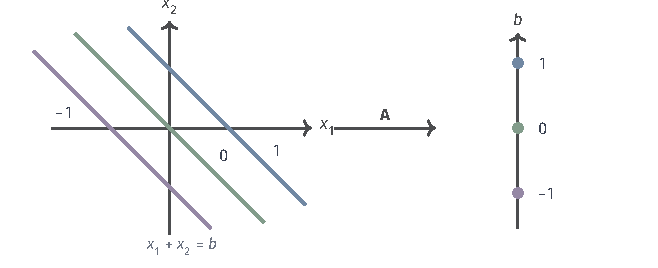
\includegraphics[width=112mm]{figures/00-shared/mathematical-preliminaries-upper/02-linear-spaces/tikz/comprehension-additions/linear-nullspace-fibers.pdf}
  \caption{同一输出对应的整组输入。对$\bm A=(1,1)$，蓝、绿、紫直线分别满足
  $x_1+x_2=1,0,-1$；右侧同色点是各直线的输出。绿色直线是$\ker\bm A$，
  其余直线是它的平移。把一整条直线归为一类后，才得到与可达输出的一一对应。}
  \label{fig:vol1-add-linear-nullspace-fibers}
\end{figure}

\section{最小二乘解}
\label{sec:ls-ordinary-ls}
\label{sec:ls-least-squares}

当$\bm b$不在列空间中时，没有输入能精确产生它。这时改求使输出误差最小的系数：
\begin{equation}
 \min_{\bm x\in\mathbb R^d}\ \lVert\bm A\bm x-\bm b\rVert_2^2 ,
 \label{eq:linear-algebra-least-squares}
\end{equation}
称为\term{最小二乘}（least squares）问题。问题中有三个对象：系数$\bm x$、拟合值$\bm A\bm x$和残差$\bm r=\bm b-\bm A\bm x$。目标只通过拟合值依赖系数，而拟合值取遍列空间，所以可以先不管系数，求列空间中离$\bm b$最近的点，这是\term{子空间最近点}问题。

由正交分解（引理~\ref{lem:ls-orthogonal-decomposition}），$\bm b$唯一地写成$\hat{\bm b}+\bm e$，其中$\hat{\bm b}\in\operatorname{range}(\bm A)$，$\bm e\perp\operatorname{range}(\bm A)$。对列空间中任一点$\bm u$，$\hat{\bm b}-\bm u$仍在列空间中，因而与$\bm e$正交，勾股关系给出
\begin{equation}
 \lVert\bm b-\bm u\rVert_2^2=\lVert\hat{\bm b}-\bm u\rVert_2^2+\lVert\bm e\rVert_2^2\geq\lVert\bm e\rVert_2^2 ,
 \label{eq:ls-nearest-point-pythagoras}
\end{equation}
等号当且仅当$\bm u=\hat{\bm b}$。所以正交投影$\hat{\bm b}$是唯一的最优拟合值，最近点也由“残差与列空间正交”完全刻画。图~\ref{fig:ls-orthogonal-projection-nearest}在一条直线子空间上画出这一几何。

\begin{figure}[htbp]
  \centering
  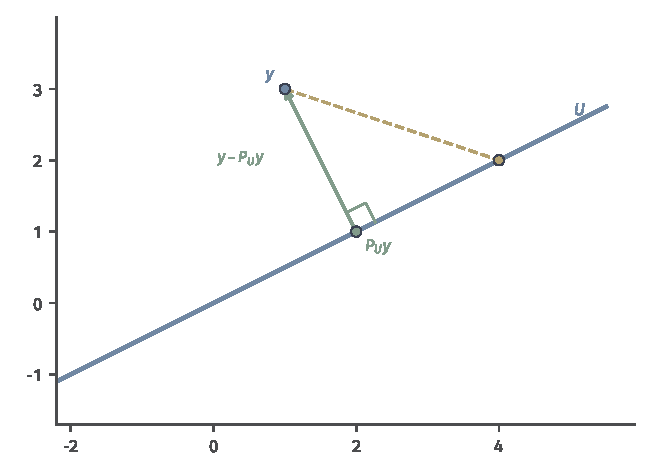
\includegraphics[width=112mm]{figures/00-shared/mathematical-preliminaries-upper/02-linear-spaces/matplotlib/ls-orthogonal-projection-nearest/ls-orthogonal-projection-nearest.pdf}
  \caption{直线子空间$U$（过原点、方向$(2,1)$）上离$\bm y=(1,3)^\top$最近的点是正交投影
  $\bm p=(2,1)^\top$，误差$\bm y-\bm p=(-1,2)^\top$与$U$垂直（直角小方块）；
  同一线上的另一候选$\bm q=(4,2)^\top$到$\bm y$的距离$\sqrt{10}$明显大于最短距离$\sqrt5$。
  这是解析式教学构造。}
  \label{fig:ls-orthogonal-projection-nearest}
\end{figure}

残差与列空间正交，就是与每一列$\bm a_j$正交，合写为$\bm A^\top\bm r=\bm0$。代入$\bm r=\bm b-\bm A\hat{\bm x}$，得到\term{正规方程}（normal equations）
\begin{equation}
 \bm A^\top\bm A\hat{\bm x}=\bm A^\top\bm b .
 \label{eq:linear-algebra-normal-equations}
\end{equation}
“正规”指法向，即残差沿列空间的法方向。由上一段，$\hat{\bm x}$是最小二乘解当且仅当它满足正规方程。这个条件完全由正交分解推出，不需要梯度、Hessian或一般最优化的一阶条件。向量$\bm A^\top\bm r$以下称为正规残差，它为零正是最小二乘的最优性条件。

拟合值随$\bm b$线性变化，可以写成投影矩阵。设$\bm Q_1$的列是$\operatorname{range}(\bm A)$的一组标准正交基，到列空间的正交投影为$\bm P=\bm Q_1\bm Q_1^\top$（第~\ref{sec:ls-projection-matrices}节），于是拟合值与残差分别是$\bm P\bm b$与$(\bm I-\bm P)\bm b$。$\bm A$满列秩时，由正规方程得$\bm A\hat{\bm x}=\bm A(\bm A^\top\bm A)^{-1}\bm A^\top\bm b$对一切$\bm b$成立，所以
\begin{equation}
 \bm P=\bm A(\bm A^\top\bm A)^{-1}\bm A^\top .
 \label{eq:ls-column-space-projector}
\end{equation}
它对称且幂等：对称说明残差与拟合值正交，幂等说明拟合值再拟合一次不变。这些是几何描述，实际求解只需要系数$\hat{\bm x}$，不必形成这个$m\times m$矩阵。

正规方程是否总有解、有多少个解，仍由列空间与零空间回答。下面的定理把最优性条件、存在性和唯一性合在一起，后面各种最小二乘算法都以它为正确性依据。

\begin{theorem}[最小二乘解的刻画]
\label{thm:ls-least-squares-solutions}
对任意$\bm A\in\mathbb R^{m\times d}$与$\bm b\in\mathbb R^m$，$\hat{\bm x}$是问题~\eqref{eq:linear-algebra-least-squares}的解当且仅当它满足正规方程~\eqref{eq:linear-algebra-normal-equations}。最小二乘解总存在，全部解为$\hat{\bm x}+\ker\bm A$，它们有相同的拟合值$\bm P\bm b$与残差。解唯一当且仅当$\bm A$满列秩，此时$\bm A^\top\bm A$正定，$\hat{\bm x}=(\bm A^\top\bm A)^{-1}\bm A^\top\bm b$。
\end{theorem}
\begin{proof}
由式~\eqref{eq:ls-nearest-point-pythagoras}，$\hat{\bm x}$最优当且仅当$\bm A\hat{\bm x}=\bm P\bm b$。$\bm A\hat{\bm x}$属于列空间，由正交分解的唯一性，这又等价于$\bm b-\bm A\hat{\bm x}\perp\operatorname{range}(\bm A)$，即正规方程。$\bm P\bm b$属于列空间，至少有一个系数向量实现它，所以解存在。若$\bm A^\top\bm A\bm x=\bm0$，则$\lVert\bm A\bm x\rVert_2^2=\bm x^\top\bm A^\top\bm A\bm x=0$，反向包含是直接的，故
\begin{equation}
 \ker(\bm A^\top\bm A)=\ker\bm A ,
 \label{eq:ls-normal-kernel}
\end{equation}
正规方程的解集是一个特解加上$\ker\bm A$，而核向量不改变$\bm A\bm x$。解唯一当且仅当$\ker\bm A=\{\bm0\}$，即满列秩；这时对$\bm x\neq\bm0$有$\bm x^\top\bm A^\top\bm A\bm x=\lVert\bm A\bm x\rVert_2^2>0$，$\bm A^\top\bm A$正定。
\end{proof}

定理区分了两层唯一性：拟合值总是唯一的，系数只在$\bm A$满列秩时唯一。相容方程是残差为零的特例：$\bm P\bm b=\bm b$，最小二乘解集就是精确解集。

\begin{example}[三条不相容观测的最佳折中]
\label{ex:ls-line-least-squares}
现在回到示例~\ref{ex:ls-line-three-cases}中无解的观测$\bm b=(1,2,2)^\top$，看最小二乘怎样在三条互相矛盾的等式之间取舍。由$\bm A^\top\bm A$与$\bm A^\top\bm b$写出正规方程
\[
 \begin{bmatrix}3&3\\3&5\end{bmatrix}\hat{\bm x}=\begin{bmatrix}5\\6\end{bmatrix},
\]
解得$\hat{\bm x}=(7/6,1/2)^\top$，拟合值为$(7/6,5/3,13/6)^\top$，残差$\bm r=\bm b-\bm A\hat{\bm x}=(-1/6,1/3,-1/6)^\top$。按定理，残差应与两列都正交：$\bm A^\top\bm r$的两个分量分别为$-\frac16+\frac13-\frac16=0$与$\frac13-\frac26=0$，确实如此。残差平方和为$1/6$，不为零。

三条观测不能同时满足，最小二乘给出它们的最佳折中：中间时刻的观测高于拟合直线，两端低于它。对相容观测$(1,2,3)^\top$，同样的正规方程给出$(1,1)^\top$与零残差，可见精确求解就是最优残差为零时的同一目标。
\end{example}

满列秩只保证系数唯一，不保证系数稳定。设计矩阵的两列接近共线时，这一点最明显。

\begin{example}[近共线设计]
\label{ex:ls-nearly-collinear-design}
下面用参数$\varepsilon$控制两列的夹角，观察系数怎样随它变化。取非零正交向量$\bm c,\bm q$，设计矩阵的两列为$\bm c$与$\bm c+\varepsilon\bm q$，观测为$\bm y=\bm c+\delta\bm q$。由$w_1\bm c+w_2(\bm c+\varepsilon\bm q)=(w_1+w_2)\bm c+\varepsilon w_2\bm q$，拟合值只依赖$w_1+w_2$与$\varepsilon w_2$。$\varepsilon\neq0$时，系数
\[
 \hat{\bm w}=\Bigl(1-\frac{\delta}{\varepsilon},\ \frac{\delta}{\varepsilon}\Bigr)^\top
\]
精确拟合$\bm y$，残差为零。$\varepsilon=0$时两列重合，只能拟合$\bm c$分量，残差跳到$\delta\bm q$，凡满足$w_1+w_2=1$的系数都是解。
\end{example}

对照三个对象：$\varepsilon\to0$时拟合值从$\bm y$突变为$\bm c$，系数则趋于无穷，并对$\varepsilon$、$\delta$极为敏感。这是近共线几何本身的性质，不是舍入造成的，第~\ref{sec:ls-ls-regularization-sensitivity}节用奇异值量化这种敏感性。

\section{最小范数解}
\label{sec:ls-select-among-solutions}

最小二乘解集$\hat{\bm x}+\ker\bm A$在秩亏时含无穷多个点，方程本身不指定其中哪一个。为报告一个确定的答案，需要额外的选解条件，最常用的是取欧氏范数最小者，称为\term{最小范数解}（minimum-norm solution）。所用的工具是输入空间的正交直和$\mathbb R^d=\operatorname{range}(\bm A^\top)\oplus\ker\bm A$（定理~\ref{thm:ls-four-subspaces-orthogonality}）：核分量不影响拟合，却增加长度，所以应当去掉。

\begin{theorem}[最小范数代表]
\label{thm:ls-minimum-norm-representative}
对任意$\bm A$与$\bm b$，最小二乘解中存在唯一的欧氏范数最小者$\bm x_\star$，它是解集中唯一落在$\operatorname{range}(\bm A^\top)$中的点。方程相容时，$\bm x_\star$是精确解中范数最小者；方程有唯一解时，$\bm x_\star$就是这个解。
\end{theorem}
\begin{proof}
把任一最小二乘解写成$\bm x=\bm x_R+\bm x_N$，$\bm x_R\in\operatorname{range}(\bm A^\top)$，$\bm x_N\in\ker\bm A$。$\bm A\bm x_R=\bm A\bm x$，去掉核分量不改变拟合值，$\bm x_R$仍是最小二乘解。两个解之差属于$\ker\bm A$，它们的行空间分量之差既在$\operatorname{range}(\bm A^\top)$中又在$\ker\bm A$中，只能为零，所以全部解共享同一个$\bm x_\star=\bm x_R$。勾股关系给出$\lVert\bm x\rVert_2^2=\lVert\bm x_\star\rVert_2^2+\lVert\bm x_N\rVert_2^2$，等号当且仅当$\bm x_N=\bm0$。相容与唯一可解的情形是特例。
\end{proof}

至此出现了三层不同的确定性。拟合值$\bm P\bm b$由$\bm b$和列空间唯一决定；系数只在满列秩时由拟合值唯一决定；秩亏时，系数的唯一性来自额外的选解条件。选取代表的依据是事先给定的欧氏范数，并没有把多解方程改成唯一可解；换一个范数，选出的点一般也会改变。

$\bm A$满行秩时，“落在行空间中”这一刻画可以直接变成公式：所求的解形如$\bm x=\bm A^\top\bm w$，代入方程得$\bm A\bm A^\top\bm w=\bm b$。

\begin{theorem}[满行秩时的最小范数解]
\label{thm:ls-min-norm-full-row-rank}
设$\bm A\in\mathbb R^{m\times d}$满行秩。则$\bm A\bm A^\top$可逆，方程$\bm A\bm x=\bm b$对每个$\bm b$相容，其最小范数解为
\begin{equation}
 \bm x_\star=\bm A^\top(\bm A\bm A^\top)^{-1}\bm b .
 \label{eq:ls-min-norm-full-row-rank}
\end{equation}
\end{theorem}
\begin{proof}
与式~\eqref{eq:ls-normal-kernel}同理，$\ker(\bm A\bm A^\top)=\ker\bm A^\top$，满行秩时它为$\{\bm0\}$，所以$\bm A\bm A^\top$可逆。右端满足$\bm A\bm x_\star=\bm b$，并且落在$\operatorname{range}(\bm A^\top)$中，由定理~\ref{thm:ls-minimum-norm-representative}，它就是最小范数解。
\end{proof}

式~\eqref{eq:ls-min-norm-full-row-rank}说明解是各行的组合，组合系数由$m$阶方程确定。计算时是形成Gram矩阵$\bm A\bm A^\top$，还是对$\bm A^\top$作QR分解，留到第~\ref{sec:ls-normal-equations-method}节与第~\ref{sec:ls-qr-method}节比较。$\bm A$既不满行秩也不满列秩时，两个满秩公式都不能用，下一节用奇异值分解写出一般秩下的统一公式。

\section{伪逆与解的表示}
\label{sec:ls-pseudoinverse}

前三节规定了各种情形的处理方式：唯一可解时取这个解，无解时取最近的拟合值，多解时取范数最小的系数。一般的$\bm A$可能既不满列秩也不满行秩，两种选择都要作。本节沿第~\ref{chap:singular-value-decomposition}章的奇异方向给出统一构造：对能够恢复的方向取逆，其他方向置为零；再用Penrose条件和两个正交投影说明这一构造不依赖分解的选取。

\subsection{伪逆的构造}
\label{sec:ls-pseudoinverse-construction}

设$\bm A$的秩为$r$，奇异值分解为$\bm A=\sum_{i=1}^r\sigma_i\bm u_i\bm v_i^\top$（式~\eqref{eq:matrix-analysis-svd-rank-one-sum}），$\sigma_1\geq\cdots\geq\sigma_r>0$，并把$\bm u_i$、$\bm v_i$分别扩充为$\mathbb R^m$与$\mathbb R^d$的标准正交基。$\bm A$把$\bm v_i$伸缩为$\sigma_i\bm u_i$，反过来自然应把$\bm u_i$送回$\bm v_i/\sigma_i$。

把$\bm b$按$\bm u_i$展开，三类分量的去向各不相同。分量$\bm u_i^\top\bm b$（$i\leq r$）是可以拟合的部分，配给输入方向$\bm v_i/\sigma_i$；$i>r$的分量落在$\operatorname{range}(\bm A)^\perp$中，没有原像，留在残差里；零空间方向$\bm v_{r+1},\ldots,\bm v_d$不分配任何分量。

\begin{definition}[Moore--Penrose伪逆]
\label{def:matrix-analysis-pseudoinverse}
$\bm A$的\term{Moore--Penrose伪逆}（Moore--Penrose pseudoinverse）为
\begin{equation}
 \bm A^\dagger=\sum_{i=1}^r\frac{1}{\sigma_i}\bm v_i\bm u_i^\top ,
 \label{eq:matrix-analysis-pseudoinverse}
\end{equation}
$\bm A=\bm0$时规定$\bm A^\dagger=\bm0$。
\end{definition}

下面的定理说明，这一构造恰好完成了最小二乘与最小范数两次选择。

\begin{theorem}[伪逆给出最小范数最小二乘解]
\label{thm:matrix-analysis-pseudoinverse-minimum-norm}
全部最小二乘解为$\bm A^\dagger\bm b+\ker\bm A$，其中$\bm x_\star=\bm A^\dagger\bm b$是唯一的最小范数解。
\end{theorem}
\begin{proof}
记$b_i=\bm u_i^\top\bm b$、$c_i=\bm v_i^\top\bm x$。由$\bm u_i$标准正交，
\[
 \lVert\bm A\bm x-\bm b\rVert_2^2
 =\sum_{i=1}^r(\sigma_ic_i-b_i)^2+\sum_{i=r+1}^m b_i^2 .
\]
第二项与$\bm x$无关，第一项当且仅当$c_i=b_i/\sigma_i$（$i\leq r$）时为零，$c_{r+1},\ldots,c_d$任取。前者正是$\bm A^\dagger\bm b$的坐标，后者组成任意核向量。$\bm A^\dagger\bm b$只含$\bm v_1,\ldots,\bm v_r$方向，与核向量正交，由定理~\ref{thm:ls-minimum-norm-representative}，它是最小范数解。
\end{proof}

定理对秩和$\bm b$的位置都没有要求，前面的公式都是它的特例。$\bm A$满列秩时核为零，最小二乘解唯一，所以$\bm A^\dagger=(\bm A^\top\bm A)^{-1}\bm A^\top$；满行秩时每个右端都相容，由式~\eqref{eq:ls-min-norm-full-row-rank}，$\bm A^\dagger=\bm A^\top(\bm A\bm A^\top)^{-1}$；$\bm A$可逆时两式都化为$\bm A^{-1}$。一般秩时两次选择都真正起作用，只有和式~\eqref{eq:matrix-analysis-pseudoinverse}可用。

显式写出逆或伪逆只是数学表达。实际计算让分解因子依次作用于右端，不形成$\bm A^\dagger$，步骤见第~\ref{sec:ls-svd-solve}节。

\begin{example}[复制常数列后的最小范数拟合]
\label{ex:ls-line-min-norm}
把示例~\ref{ex:ls-line-three-cases}的两种缺陷合在一起：既复制常数列，又使用不相容的观测，
\[
 \widetilde{\bm A}=\begin{bmatrix}1&0&1\\1&1&1\\1&2&1\end{bmatrix},\qquad \bm b=(1,2,2)^\top .
\]
这时最小二乘解不唯一，需要最小范数来选出代表。拟合值$\widetilde{\bm A}\bm x=(x_1+x_3)\bm a_1+x_2\bm a_2$只依赖两个常数系数之和，所以最佳拟合值与示例~\ref{ex:ls-line-least-squares}相同，全部最小二乘解满足$x_1+x_3=7/6$、$x_2=1/2$，即$(7/6-t,\,1/2,\,t)^\top$，$t\in\mathbb R$。在这条直线上找离原点最近的点：范数平方$(7/6-t)^2+t^2+1/4$在$t=7/12$时最小，最小范数代表为$\bm x_\star=(7/12,1/2,7/12)^\top$。

这个代表与核方向$(1,0,-1)^\top$的内积为$7/12-7/12=0$，正如定理所说落在行空间中。两次选择的分工由此可见：最小二乘选定拟合值，最小范数再在实现它的系数中，把常数项平均分给两个相同的列。
\end{example}

\subsection{Penrose条件与正交投影}
\label{sec:ls-penrose-conditions}

奇异向量不唯一，例如重奇异值对应的奇异向量可以在子空间内任意旋转。要说明$\bm A^\dagger$与所选分解无关，需要不提奇异向量、又能唯一确定它的条件。

\begin{theorem}[Penrose条件]
\label{thm:ls-penrose-conditions}
$\bm G=\bm A^\dagger$满足
\[
\begin{gathered}
\bm A\bm G\bm A=\bm A,\qquad
\bm G\bm A\bm G=\bm G,\\
(\bm A\bm G)^\top=\bm A\bm G,\qquad
(\bm G\bm A)^\top=\bm G\bm A ,
\end{gathered}
\]
并且满足这四个条件的$\bm G\in\mathbb R^{d\times m}$只有一个。
\end{theorem}
\begin{proof}
由和式与奇异向量的标准正交性，$\bm A\bm A^\dagger=\sum_{i\leq r}\bm u_i\bm u_i^\top$，$\bm A^\dagger\bm A=\sum_{i\leq r}\bm v_i\bm v_i^\top$，二者对称，再右乘$\bm A$或$\bm A^\dagger$即得前两条。反过来设$\bm G$满足四个条件。由第一条，$\bm A\bm G$幂等且$\operatorname{range}(\bm A\bm G)=\operatorname{range}(\bm A)$，再由第三条，它是到$\operatorname{range}(\bm A)$的正交投影；同理$\bm G\bm A$是对称幂等矩阵，零空间为$\ker\bm A$，因而是到$(\ker\bm A)^\perp$的正交投影。正交投影由子空间唯一决定，所以$\bm A\bm G=\bm A\bm A^\dagger$、$\bm G\bm A=\bm A^\dagger\bm A$，于是
\[
 \bm G=\bm G\bm A\bm G=\bm A^\dagger\bm A\bm G=\bm A^\dagger\bm A\bm A^\dagger=\bm A^\dagger .
\]
\end{proof}

四个条件不必死记。前两条是在可恢复方向上的一致性：第一条说明，对能实现的输出$\bm y=\bm A\bm x$，$\bm G\bm y$确实实现它；第二条说明，$\bm G$的输出不含被$\bm A$消去的多余成分。只有前两条时，$\bm A\bm G$与$\bm G\bm A$是幂等矩阵，但可以是斜投影；后两条的对称性要求它们是正交投影，分别对应“取最近的拟合值”和“取范数最小的系数”。正因为四个条件不涉及奇异向量，$\bm A^\dagger$不依赖奇异值分解的选取。

由证明，$\bm A\bm A^\dagger$是到列空间的正交投影，$\bm A^\dagger\bm A$是到行空间$\operatorname{range}(\bm A^\top)$的正交投影。两次选择因此写成两个可以检查的等式：$\bm A\bm x_\star=\bm A\bm A^\dagger\bm b=\bm P\bm b$说明拟合值是$\bm b$在列空间上的投影，$\bm A^\dagger\bm A\bm x_\star=\bm x_\star$说明$\bm x_\star$不含零空间分量。

在示例~\ref{ex:ls-line-min-norm}中，$\widetilde{\bm A}\bm x_\star=(7/6,5/3,13/6)^\top$与示例~\ref{ex:ls-line-least-squares}的拟合值相同；$\bm x_\star=\frac7{12}(1,0,1)^\top+\frac12(0,1,0)^\top$是$\widetilde{\bm A}$的两行之组合，已在行空间中，投影不改变它。

统一公式也暴露了一个代价：小正奇异值取倒数后增益$1/\sigma_i$很大，数据误差会被放大。第~\ref{sec:ls-numerical-sensitivity}节再量化这一敏感性；这里先完成各类解的统一表达，为随后选择计算方法提供目标。

\section{加权最小二乘}
\label{sec:ls-weighted-ls}

前面都用欧氏长度度量残差，各坐标同等对待。不同观测的可靠程度不同，或观测误差彼此相关时，应按给定的权重度量残差。给定对称正定$\bm M\in\mathbb R^{m\times m}$，\term{加权最小二乘}（weighted least squares）问题为
\begin{equation}
 \min_{\bm x}\ (\bm A\bm x-\bm b)^\top\bm M(\bm A\bm x-\bm b).
 \label{eq:ls-weighted-objective}
\end{equation}

权矩阵的两类元素分别改变目标的不同方面。$\bm M=\operatorname{diag}(m_1,\ldots,m_m)$时目标为$\sum_im_ir_i^2$，$m_i$越大，第$i$个观测的误差越昂贵，拟合值就越被拉向这个观测；这适合观测精度不同的情形。非对角元引入交叉项$2m_{ij}r_ir_j$，使惩罚依赖残差的方向组合。例如$\bm M=\begin{bmatrix}2&-1\\-1&2\end{bmatrix}$时，残差$(1,1)^\top$的代价为$2$，残差$(1,-1)^\top$的代价为$6$：两个观测同向偏离被看得较轻，反向偏离被看得较重，这适合两个观测的误差倾向于一起偏移的情形。怎样由误差的统计性质选出$\bm M$，不在本章讨论。

由Gram因子（定理~\ref{thm:ls-gram-factor}）或正定平方根（第~\ref{sec:ls-matrix-square-root}节），可写$\bm M=\bm R^\top\bm R$，$\bm R$可逆，于是目标等于$\lVert\bm R\bm A\bm x-\bm R\bm b\rVert_2^2$。这一步称为\term{白化}（whitening）：先把各坐标的误差变换到同一欧氏尺度，加权问题就成为$\bm R\bm A$、$\bm R\bm b$上的普通最小二乘，定理~\ref{thm:ls-least-squares-solutions}的结论都可以搬过来。

\begin{theorem}[加权最小二乘解的刻画]
\label{thm:ls-weighted-least-squares}
设$\bm M\in\mathbb R^{m\times m}$对称正定。则$\hat{\bm x}$是问题~\eqref{eq:ls-weighted-objective}的解当且仅当它满足加权正规方程
\begin{equation}
 \bm A^\top\bm M(\bm b-\bm A\hat{\bm x})=\bm0 .
 \label{eq:linear-algebra-weighted-normal-equations}
\end{equation}
这组方程总有解，全部解为$\hat{\bm x}+\ker\bm A$；解唯一当且仅当$\bm A$满列秩。
\end{theorem}
\begin{proof}
对$\bm R\bm A$与$\bm R\bm b$应用定理~\ref{thm:ls-least-squares-solutions}：$\hat{\bm x}$最优当且仅当$(\bm R\bm A)^\top(\bm R\bm b-\bm R\bm A\hat{\bm x})=\bm0$，由$\bm R^\top\bm R=\bm M$，这正是式~\eqref{eq:linear-algebra-weighted-normal-equations}。解存在，解集是一个特解加上$\ker(\bm R\bm A)$；$\bm R$可逆，故$\ker(\bm R\bm A)=\ker\bm A$。
\end{proof}

加权正规方程说明残差在$\bm M$内积下与列空间正交。权矩阵改变的是误差的度量，不改变系数和拟合值的含义。若$\bm M$只是半正定，$\ker\bm M$中的残差分量不受惩罚，$\bm R$奇异，唯一性要求$\ker(\bm M\bm A)=\{\bm0\}$，拟合值本身也可能不唯一，正定版本的结论不能全部沿用。

$\bm A$满列秩时，加权拟合值为$\bm P_{\bm M}\bm b$，其中$\bm P_{\bm M}=\bm A(\bm A^\top\bm M\bm A)^{-1}\bm A^\top\bm M$。它幂等，一般不对称，在欧氏内积下是斜投影。但对任意$\bm u,\bm v$，$\bm u^\top\bm M\bm P_{\bm M}\bm v=\bm u^\top\bm M\bm A(\bm A^\top\bm M\bm A)^{-1}\bm A^\top\bm M\bm v$关于$\bm u,\bm v$对称，所以$\bm P_{\bm M}$在$\bm M$内积下自伴，是该内积下的正交投影。同一组$\bm A,\bm b$换用不同权矩阵，最近点随之移动，如下例与图~\ref{fig:linear-algebra-weighted-projection}所示。

白化只变换观测端，未知量和它的欧氏范数都不变，所以加权问题与白化后普通问题的解集相同。秩亏时，最小范数代表仍按原系数的欧氏范数选取，即白化后问题的$(\bm R\bm A)^\dagger\bm R\bm b$；构造权因子并调用求解方法的步骤见第~\ref{sec:ls-svd-solve}节。

\begin{example}[同一直线上的两种最近点]
\label{ex:linear-algebra-weighted-projection}
用最简单的单列情形比较两种内积下的最近点。取$\bm A=(1,1)^\top$、$\bm b=(2,1)^\top$，拟合值都形如$a(1,1)^\top$。欧氏正规方程为$2a=3$，最近点是$(1.5,1.5)^\top$，坐标取两个观测的平均。改用$\bm M=\operatorname{diag}(1,4)$后，加权正规方程$\bm A^\top\bm M\bm A\,a=\bm A^\top\bm M\bm b$成为$5a=6$，最近点移到$(1.2,1.2)^\top$：第二个坐标的误差代价更大，最近点向$b_2=1$靠近。

加权解的残差$(0.8,-0.2)^\top$与$(1,1)^\top$的欧氏内积为$0.6$，加权内积却是$0.8-4\times0.2=0$。残差只在所选的内积下与列空间正交；若用欧氏内积去检查加权解，会误以为它不满足最优条件。
\end{example}

\begin{figure*}[htbp]
  \centering
  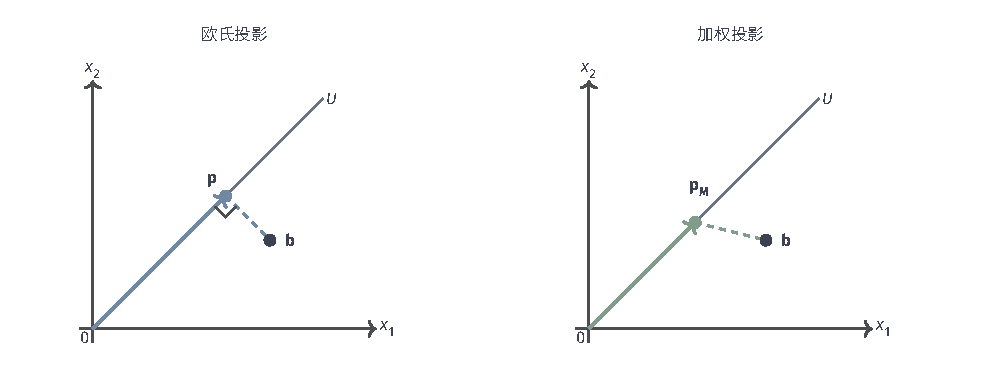
\includegraphics[width=168.998mm]{figures/00-shared/mathematical-preliminaries-upper/02-linear-spaces/tikz/linear-algebra-weighted-projection/figure.pdf}
  \caption{同一目标在同一直线上的欧氏投影与加权投影。实箭头是投影向量，虚线是残差；
  右图画在普通坐标中，残差不必形成欧氏直角。正交性必须用所选内积判断。}
  \label{fig:linear-algebra-weighted-projection}
\end{figure*}

\section{齐次最小二乘}
\label{sec:linear-algebra-homogeneous-estimation}

另一类拟合问题的模型写成$\bm A\bm h\approx\bm0$，只确定参数的比例。例如用直线$h_1u+h_2v+h_3=0$拟合平面上的点$(u_j,v_j)$，每个点给出一行$[\,u_j\ v_j\ 1\,]$，$\bm h$乘以非零常数描述同一条直线。直接最小化$\lVert\bm A\bm h\rVert_2^2$总得到无意义的$\bm h=\bm0$，所以必须先固定尺度。

固定一个分量，例如$h_3=1$，会把问题化为普通最小二乘；但真实直线过原点时$h_3=0$，这一归一化恰好排除了它。固定欧氏长度则对各分量一视同仁，得到\term{齐次最小二乘}（homogeneous least squares）问题
\begin{equation}
 \min_{\lVert\bm h\rVert_2=1}\ \lVert\bm A\bm h\rVert_2^2
 =\min_{\lVert\bm h\rVert_2=1}\bm h^\top\bm A^\top\bm A\bm h .
 \label{eq:linear-algebra-homogeneous-least-squares}
\end{equation}
它与求齐次方程$\bm A\bm h=\bm0$的全部解不同：后者的解集是子空间$\ker\bm A$，满列秩时只含零向量；前者总给出一个最接近满足的单位方向。右端是对称半正定矩阵$\bm A^\top\bm A$的二次型在单位向量上的最小值，由第~\ref{chap:singular-value-decomposition}章构造奇异值分解时所用的特征基即可求出。

\begin{theorem}[齐次最小二乘的最优解]
\label{thm:ls-homogeneous-minimizers}
设$\lambda_{\min}$为$\bm A^\top\bm A$的最小特征值。则问题~\eqref{eq:linear-algebra-homogeneous-least-squares}的最小值存在且等于$\lambda_{\min}$，最优解恰为特征空间$\ker(\bm A^\top\bm A-\lambda_{\min}\bm I)$中的单位向量。$\lambda_{\min}$单重时最优解只差一个符号；$\ker\bm A\neq\{\bm0\}$时$\lambda_{\min}=0$，任一单位零空间向量都是最优解。
\end{theorem}
\begin{proof}
取$\bm A^\top\bm A$的标准正交特征基$\bm v_1,\ldots,\bm v_d$，特征值$\lambda_1\geq\cdots\geq\lambda_d=\lambda_{\min}\geq0$，这正是构造奇异值分解时所用的右奇异向量。单位向量写成$\bm h=\sum_ic_i\bm v_i$，$\sum_ic_i^2=1$，则
\[
 \bm h^\top\bm A^\top\bm A\bm h=\sum_{i=1}^d\lambda_ic_i^2\geq\lambda_{\min}\sum_{i=1}^dc_i^2=\lambda_{\min},
\]
取$\bm h=\bm v_d$时等号成立，所以最小值存在且等于$\lambda_{\min}$。等号成立当且仅当$\lambda_i>\lambda_{\min}$的系数$c_i$都为零，即$\bm h$属于$\lambda_{\min}$的特征空间。特征空间一维时其中的单位向量只有一对$\pm\bm h_\star$。由式~\eqref{eq:ls-normal-kernel}，$\ker\bm A=\ker(\bm A^\top\bm A)$；它非零时$0$是特征值，而半正定矩阵的特征值非负，故$\lambda_{\min}=0$。
\end{proof}

用$\bm A=[\,1\ -2\,]$核验：$\bm A^\top\bm A$的特征值为$0$与$5$，最小特征值的单位特征向量为$\pm(2,1)^\top/\sqrt5$，它满足$h_1-2h_2=0$，残差为零，两个符号给出同一比例$h_1:h_2=2:1$。

换成奇异值的语言，右奇异向量是$\bm A^\top\bm A$的单位特征向量，特征值为奇异值的平方（$d>r$时补上零），所以最优解就是最小奇异值对应的右奇异子空间中的单位向量，最小值为最小奇异值的平方。同类的长度约束极值在第~\ref{sec:ls-rayleigh-extremal}节推广为Rayleigh商的一般结论。

最小特征值接近重根时，任意小的数据扰动都可能从近似最优的子空间中选出不同的方向，最优方向的敏感度由第~\ref{sec:ls-subspace-sensitivity}节的子空间界控制。这里只说明解的性质，用SVD选取具体单位向量的步骤见第~\ref{sec:ls-svd-solve}节。

\section{解的检验条件}
\label{sec:ls-least-squares-verification}

算出候选解以后，要用与目标对应的条件核对它。不同目标的条件不同，用错条件会把正确的解判为失败，或把不满足目标的解当作成功。下面依次列出各目标的条件，对象都是候选解$\bm x$及其原残差$\bm r=\bm b-\bm A\bm x$。

精确方程检查原残差：$\bm r=\bm0$。这只对相容方程适用；方程是否相容由式~\eqref{eq:ls-augmented-rank}判断，而不是由残差能否降到零来猜测。

普通最小二乘检查正规残差：$\bm A^\top\bm r=\bm0$，同时报告残差范数$\lVert\bm r\rVert_2$，它是$\bm b$到列空间的距离。无解方程的最优残差本来就不为零：示例~\ref{ex:ls-line-least-squares}的残差范数为$1/\sqrt6$，它满足$\bm A^\top\bm r=\bm0$，并不说明求解失败。

要求最小范数解时，再检查行空间条件：$\bm x\perp\ker\bm A$，等价地，$\bm A^\dagger\bm A\bm x=\bm x$，或$\bm x=\bm A^\top\bm w$对某个$\bm w$成立。秩亏时系数不唯一本身也不是失败：示例~\ref{ex:ls-line-min-norm}中，$(7/6-t,1/2,t)^\top$对每个$t$都满足正规残差为零，若只要求最小二乘，它们都是合格答案；只有$t=7/12$还满足行空间条件。

加权问题核对$\bm A^\top\bm M\bm r=\bm0$，报告$\sqrt{\bm r^\top\bm M\bm r}$并说明所用的权矩阵；示例~\ref{ex:linear-algebra-weighted-projection}中欧氏的$\bm A^\top\bm r=0.6\neq0$，这不是错误。齐次拟合不能照搬$\bm A^\top\bm r=\bm0$，否则只会把解推向零向量；应检查$\lVert\bm h\rVert_2=1$，并确认$\bm h$是$\bm A^\top\bm A$最小特征值的特征方向。

这些条件规定了后续算法应该达到什么。浮点计算中“为零”要换成相对容限，容限怎样确定、残差小能否保证误差小，在第~\ref{sec:ls-numerical-stability}节讨论；直接法的分解质量与迭代法的停止条件分别见第~\ref{sec:ls-direct-method-comparison}节、第~\ref{sec:ls-stationary-stopping}节和第~\ref{sec:ls-krylov-stopping}节。

\FloatBarrier
\section{本章小结}
\label{sec:solution-selection-chapter-summary}

本章回答了反求输入时要求什么样的解。方程$\bm A\bm x=\bm b$相容当且仅当$\bm b\in\operatorname{range}(\bm A)$，即$\operatorname{rank}[\bm A\;\bm b]=\operatorname{rank}\bm A$；相容时全部解是一个特解加上$\ker\bm A$，自由度为$d-\operatorname{rank}\bm A$。方程个数与未知量个数不能单独决定这些情况，满列秩只保证至多一解，满行秩只保证有解。

无解时改求最小二乘解。由正交分解，最优拟合值是$\bm b$在列空间上的正交投影，总存在且唯一；系数是最小二乘解当且仅当正规残差$\bm A^\top(\bm b-\bm A\bm x)$为零，全部解为一个解加上$\ker\bm A$，只在满列秩时唯一。近共线的例子说明，系数唯一不等于系数稳定。

解不唯一时，用欧氏范数作额外的选解条件：最小范数解唯一，并且是解集中唯一落在行空间$\operatorname{range}(\bm A^\top)$中的点。伪逆$\bm A^\dagger$沿正奇异值方向取逆、其余方向置零，$\bm A^\dagger\bm b$同时完成最小二乘与最小范数两次选择；四个Penrose条件不提奇异向量就唯一确定它，$\bm A\bm A^\dagger$与$\bm A^\dagger\bm A$分别是到列空间与行空间的正交投影。小奇异值取倒数会放大数据误差，这是统一公式的边界。

加权最小二乘改变残差的度量：对称正定权矩阵经白化化为普通问题，最优条件变为$\bm A^\top\bm M\bm r=\bm0$，最小范数代表仍按原系数的欧氏范数选取。齐次最小二乘改变约束：在单位长度下最小化$\lVert\bm A\bm h\rVert_2$，解是最小奇异值对应的右奇异方向，它不同于求$\ker\bm A$中的全部解。

各目标都对应可以核对的条件：精确方程看原残差，最小二乘看正规残差，最小范数再看行空间条件，加权与齐次问题按各自的度量和约束检查。残差非零或系数不唯一都可能是正确结果。本章只确定目标；第~\ref{chap:direct-linear-solvers}章起讨论怎样计算这些解，第~\ref{chap:solution-error-regularization}章讨论在误差下如何判断结果的可信程度。

\chapter{线性方程的直接求解}
\label{sec:ls-direct-methods}
\label{chap:direct-linear-solvers}

第~\ref{chap:linear-solution-selection}章回答了“要求哪一个解”。对非奇异方阵，所求的是唯一的精确解$\bm x_\star=\bm A^{-1}\bm b$。但这只是解的表达式：先求逆再相乘要多做运算，也不必要。本章研究怎样不求逆，在有限步内把精确解算出来，并让同一次分解服务于多个右端。最小二乘问题的直接求解在第~\ref{chap:direct-least-squares-solvers}章讨论。

本章的共同做法是用消元把一般方阵化为三角方程，三角方程可以逐个分量代入求解。这类在精确算术下经有限步给出答案的方法称为直接法，它们与第~\ref{chap:stationary-iterations}章起的迭代法相对。

第~\ref{sec:ls-gaussian-elimination}节先用初等行变换说明消元的手算过程：化为阶梯形，读出主元与自由变量，并用同样的过程求逆。随后三节按矩阵结构选择分解：一般非奇异方阵用带部分选主元的LU分解，对称正定矩阵用Cholesky分解，对称不定矩阵用分块LDL分解。第~\ref{sec:ls-woodbury}节说明矩阵只作低秩修改时，怎样复用已有的分解，只多解一个低阶方程。最后一节按矩阵结构归纳方法选择，并用原始数据核验结果。

本章依赖前文的两类结果：三角分解的存在性要用到行列式，Cholesky分解要用到正定矩阵（第~\ref{sec:ls-positive-definite}节）。各算法的正确性在本章证明，稳定性只给出算法层面的结论，例如主元增长；前向误差、后向误差的系统分析在第~\ref{chap:solution-error-regularization}章展开。

记号沿用第~\ref{chap:linear-solution-selection}章：已知非奇异方阵$\bm A\in\mathbb R^{d\times d}$与$\bm b\in\mathbb R^d$，未知量为$\bm x\in\mathbb R^d$，精确解记作$\bm x_\star$。每个算法都以$\bm A$、$\bm b$为输入，以$\bm x$为输出；分解因子、置换和中间向量只是中间量，主元策略等需要预先选定的规则单独说明。若干右端排成$\bm B=[\bm b_1\;\cdots\;\bm b_s]$时，方程写成$\bm A\bm X=\bm B$，各列分别求解并共用同一次分解。

除第~\ref{sec:ls-gaussian-elimination}节外，每种算法都分三部分讲解：主要思想从需要满足的等式推导计算公式；算法实现按计算次序写出步骤，并给出可以逐步复算的算例；算法分析说明结果为什么正确、在什么条件下可以进行，以及计算代价与数值上的注意事项。

\section{Gauss消元与阶梯形}
\label{sec:ls-gaussian-elimination}

后面几节的分解都建立在消元之上。本节先把消元当作手算过程讲清：用第~\ref{sec:ls-elementary-row-operations}节的三种初等行变换把矩阵化为阶梯形，从中读出方程的解，并用同样的过程求逆矩阵。这里只关心精确算术下的结果；怎样把消元过程记录成因子以便复用，以及怎样选主元以控制舍入误差，从第~\ref{sec:ls-lu}节开始讨论。

\subsection{阶梯形与行最简形}
化简时从左到右逐列寻找\term{主元}（pivot）。在当前列尚未使用的行中找一个非零元素；必要时交换行，把它移到当前行，再用它消去同列下方的元素。若该列在余下各行全为零，就跳过这一列，继续向右。

重复到没有可用的行或列为止，得到\term{行阶梯形}（row echelon form）：零行位于底部，每个非零行的首个非零元位于上一行首个非零元的右侧。再把每个主元化为$1$，并消去主元上方的元素，就得到\term{行最简形}（reduced row echelon form）。

阶梯形中主元的个数就是原矩阵的秩。一方面，各步行变换合起来是左乘一个可逆矩阵，不改变矩阵的秩；另一方面，阶梯形的各非零行首元所在的列互不相同、依次右移，这些行线性无关，所以阶梯形的秩等于非零行数，也就是主元个数。第~\ref{sec:ls-solution-cases}节用秩判断方程是否有解，实际计算时就是这样读出秩的。

\subsection{用消元解方程}
解方程$\bm A\bm x=\bm b$时，把右端项作为最后一列附在$\bm A$后面，得到增广矩阵$[\bm A\mid\bm b]$，每次对整行执行同一操作。

三种行变换分别对应交换两个等式、将等式乘以非零数、把一个等式的倍数加到另一个等式上。这些操作不改变解，而且可以撤销，所以新方程组与原方程组的解完全相同。化到阶梯形以后，主元列对应的未知量由方程确定，没有主元的列对应可以任意取值的自由变量。

下面的例子中，第一列的首个元素为零，并且有一列没有主元。
\begin{example}[换行、消元与自由变量]
\label{ex:ls-elementary-row-reduction}
考虑以下增广矩阵。第一列的首个元素为零，先交换前两行：
\[
 \left[\begin{array}{ccc|c}0&1&2&3\\1&2&4&6\\2&4&8&12\end{array}\right]
 \longrightarrow
 \left[\begin{array}{ccc|c}1&2&4&6\\0&1&2&3\\2&4&8&12\end{array}\right].
\]
再把第三行减去第一行的两倍，消去第三行的第一列：
\[
 \left[\begin{array}{ccc|c}1&2&4&6\\0&1&2&3\\2&4&8&12\end{array}\right]
 \longrightarrow
 \left[\begin{array}{ccc|c}1&2&4&6\\0&1&2&3\\0&0&0&0\end{array}\right].
\]
这已是阶梯形。将第一行减去第二行的两倍，得到行最简形
\[
 \left[\begin{array}{ccc|c}1&0&0&0\\0&1&2&3\\0&0&0&0\end{array}\right].
\]
第一、二列是主元列，第三列没有主元。令自由变量$x_3=t$，便读出
\[
 x_1=0,\qquad x_2=3-2t,\qquad x_3=t ;
\]
任意实数$t$都给出原方程组的一个解。

最后的零行
表示$0=0$，不增加约束。若出现系数全为零而右端非零的行，方程组就无解。
\end{example}

这个例子中系数矩阵有两个主元，秩为$2$，比未知量个数少$1$，解集正好带一个自由参数。这与第~\ref{sec:ls-solution-cases}节的结论一致：相容时解集是特解加上零空间，自由参数的个数等于未知量个数减去秩。

\subsection{用消元求逆}
对$n$阶方阵$\bm A$，逆矩阵的第$j$列是方程$\bm A\bm x=\bm e_j$的解（第~\ref{sec:prelim-inverse-matrices}节）。这$n$个方程的系数矩阵相同，消元步骤只由$\bm A$决定，可以一并处理：把$\bm A$与单位矩阵并排，得到$[\bm A\mid\bm I_n]$，对整个增广矩阵作行变换，力求把左侧化为$\bm I_n$。

为什么最后右侧就是逆矩阵？若左侧最终化为$\bm I_n$，各步初等矩阵的乘积记为$\bm E$，它是可逆矩阵，并满足$\bm E\bm A=\bm I_n$；右侧则变为$\bm E\bm I_n=\bm E$。由$\bm E$可逆得$\bm A=\bm E^{-1}$，从而$\bm A\bm E=\bm I_n$。所以右侧的$\bm E$就是$\bm A^{-1}$：
\begin{equation}
 [\bm A\mid\bm I_n]\longrightarrow[\bm I_n\mid\bm A^{-1}].
 \label{eq:ls-gauss-jordan-inverse}
\end{equation}

如果化简时某一列找不到主元，左侧的阶梯形会出现零行，不能化为$\bm I_n$。这时$\bm A$没有逆：若$\bm A$可逆，则$\bm E\bm A$作为两个可逆矩阵之积也可逆；但有零行的矩阵左乘任何矩阵，结果的那一行仍是零，不可能等于$\bm I_n$。

求逆相当于一次解$n$个方程。只需要一个方程的解时，直接对$[\bm A\mid\bm b]$消元即可，先求逆再乘以$\bm b$反而多做运算。

\section{LU分解}
\label{sec:ls-lu}

一般非奇异方阵没有对称性或正定性可以利用，最基本的求解方式是第~\ref{sec:ls-gaussian-elimination}节的Gauss消元。本节把消元过程记录成两个三角因子，使求解化为两次三角代入；行交换用来避开零主元和过小的主元，因子一旦算出，换右端时可以直接复用。

\subsection{主要思想}
设$\bm A\in\mathbb R^{d\times d}$非奇异，$\bm b\in\mathbb R^d$，要求$\bm A\bm x=\bm b$的唯一精确解$\bm x_\star$。假设已经得到\term{LU分解}
\begin{equation}
 \bm P\bm A=\bm L\bm U,
 \label{eq:ls-palu}
\end{equation}
其中$\bm P$是置换矩阵，$\bm L$是单位下三角矩阵（对角元都为$1$），$\bm U$是非奇异上三角矩阵。这三个矩阵怎样由Gauss消元算出，留到下一小节；本小节说明有了分解以后怎样求出$\bm x$。

把方程$\bm A\bm x=\bm b$两边左乘$\bm P$，得$\bm P\bm A\bm x=\bm P\bm b$。左乘置换矩阵只是重排方程的先后次序，不改变解。记$\bm c=\bm P\bm b$，代入分解，方程成为
\[
 \bm L\bm U\bm x=\bm c .
\]
令$\bm y=\bm U\bm x$，它又写成$\bm L\bm y=\bm c$。所以求解分两步：先由$\bm L\bm y=\bm c$求出$\bm y$，再由$\bm U\bm x=\bm y$求出$\bm x$。两个方程的系数矩阵都是三角矩阵，可以逐个分量求解。

\paragraph{前代：求解$\bm L\bm y=\bm c$}
为了让公式也能用于对角元不为$1$的下三角矩阵（例如第~\ref{sec:ls-cholesky}节的Cholesky因子），先设$\bm L$是对角元都不为零的一般下三角矩阵。按行写出$\bm L\bm y=\bm c$：
\[
 \begin{aligned}
 l_{1,1}y_1&=c_1,\\
 l_{2,1}y_1+l_{2,2}y_2&=c_2,\\
 &\ \,\vdots\\
 l_{d,1}y_1+l_{d,2}y_2+\cdots+l_{d,d}y_d&=c_d .
 \end{aligned}
\]
第一个方程只含$y_1$，得$y_1=c_1/l_{1,1}$。第二个方程中$y_1$已经求出，移项后得$y_2=(c_2-l_{2,1}y_1)/l_{2,2}$。一般地，第$i$个方程是
\[
 \sum_{j<i}l_{i,j}y_j+l_{i,i}y_i=c_i ,
\]
其中$y_1,\ldots,y_{i-1}$已由前面的方程求出。把它们移到右边，再除以$l_{i,i}$，得
\begin{equation}
 y_i=\frac{c_i-\sum_{j<i}l_{i,j}y_j}{l_{i,i}}\qquad(i=1,2,\ldots,d).
 \label{eq:ls-forward-substitution}
\end{equation}
按$i=1,2,\ldots,d$的顺序计算，右侧用到的都是已经算出的分量。这种求解顺序称为\term{前代}；只要对角元都不为零，它逐个唯一地给出解。LU中$l_{i,i}=1$，公式化为$y_i=c_i-\sum_{j<i}l_{i,j}y_j$，不需要除法。

\paragraph{回代：求解$\bm U\bm x=\bm y$}
$\bm U$非奇异，它的行列式是对角元之积，所以对角元都不为零。按行写出$\bm U\bm x=\bm y$：
\[
 \begin{aligned}
 u_{1,1}x_1+u_{1,2}x_2+\cdots+u_{1,d}x_d&=y_1,\\
 &\ \,\vdots\\
 u_{d-1,d-1}x_{d-1}+u_{d-1,d}x_d&=y_{d-1},\\
 u_{d,d}x_d&=y_d .
 \end{aligned}
\]
这次最后一个方程只含$x_d$，得$x_d=y_d/u_{d,d}$。倒数第二个方程中$x_d$已经求出，得$x_{d-1}=(y_{d-1}-u_{d-1,d}x_d)/u_{d-1,d-1}$。一般地，第$i$个方程是
\[
 u_{i,i}x_i+\sum_{j>i}u_{i,j}x_j=y_i ,
\]
其中$x_{i+1},\ldots,x_d$已由后面的方程求出，移项后除以$u_{i,i}$，得
\begin{equation}
 x_i=\frac{y_i-\sum_{j>i}u_{i,j}x_j}{u_{i,i}}\qquad(i=d,d-1,\ldots,1).
 \label{eq:ls-back-substitution}
\end{equation}
按$i=d,d-1,\ldots,1$的顺序计算，这种求解顺序称为\term{回代}。

图~\ref{fig:ls-triangular-substitution-order}对比了两种顺序：前代自上而下，每个分量只依赖它上方已求出的分量；回代自下而上，依赖关系正好反过来。后面各节遇到三角方程时，直接调用前代和回代。分解只依赖$\bm A$，换一个右端只需重新做这两次代入。

\begin{figure}[!htb]
  \centering
  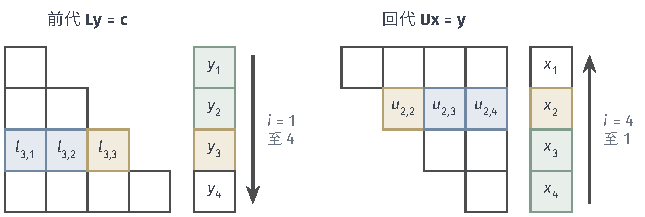
\includegraphics[width=109.1mm]{figures/01-basic-mathematics/03-vectors-matrices-and-multivariate-functions/tikz/c5-triangular-substitution-order/figure.pdf}
  \caption{前代与回代的计算顺序。左为四阶下三角方程，计算$y_3$时只用到第三行的蓝色元素与绿色的已算分量$y_1,y_2$；
  右为上三角方程，计算$x_2$时只用到$x_3,x_4$。黄色是当前用作除数的对角元与正在计算的分量，箭头是计算方向。}
  \label{fig:ls-triangular-substitution-order}
\end{figure}

\subsection{算法实现}
\label{sec:ls-lu-implementation}
输入是$\bm A$与$\bm b$，输出是$\bm x$。需要预先选定的规则是主元策略，本小节固定使用\term{部分选主元}：在当前列尚未处理的元素中选绝对值最大者作主元，绝对值相同时取行号最小者，使给定数据下的计算过程可以复算。算法由三个模块组成，下面依次给出：LU分解由$\bm A$算出$\bm P\bm A=\bm L\bm U$，前代求出$\bm y$，回代求出$\bm x$。下面逐个写出各模块的步骤，并在每一步用
\[
 \bm A=\begin{bmatrix}1&3&4\\2&2&4\\1&2&5\end{bmatrix},\qquad
 \bm b=\begin{bmatrix}2\\4\\4\end{bmatrix}
\]
演示该步的计算。

\subsubsection{LU分解}
输入$\bm A$，输出$\bm P$、$\bm L$、$\bm U$。消元逐列进行，用$k$记当前处理的列。计算中维护三个矩阵：工作矩阵$\bm W$逐步化为上三角形状，$\bm L$收集乘子，$\bm P$记录行交换。下面每一步之后都给出例中这三个矩阵的当前值。
\begin{enumerate}
 \item \textbf{初始化。}令$\bm W=\bm A$，$\bm L=\bm I_d$，$\bm P=\bm I_d$，$k=1$。

 例中
 \[
  \bm W=\begin{bmatrix}1&3&4\\2&2&4\\1&2&5\end{bmatrix},\quad
  \bm L=\begin{bmatrix}1&0&0\\0&1&0\\0&0&1\end{bmatrix},\quad
  \bm P=\begin{bmatrix}1&0&0\\0&1&0\\0&0&1\end{bmatrix}.
 \]

 \item \textbf{选主元并换行。}在第$k$列的第$k$至$d$行中找出主元所在的行
 \[
  r=\operatorname*{arg\,max}_{k\leq i\leq d}|w_{i,k}| ,
 \]
 交换$\bm W$的第$k,r$两行，并对$\bm P$作同样的行交换；$\bm L$前$k-1$列已经保存的乘子也交换这两行，使它们始终跟随所在的方程（理由见本节的算法分析）。若选出的主元为零，说明输入不满足非奇异的前提，停止并报告本算法不适用；$\bm A$非奇异时这种情况不会出现，理由见定理~\ref{thm:ls-lu-existence}。

 例中$k=1$，第一列为$(1,2,1)^\top$，绝对值最大的在第二行，$r=2$。交换$\bm W$与$\bm P$的第一、二行；$\bm L$的前$k-1=0$列中还没有乘子，不变：
 \[
  \bm W=\begin{bmatrix}2&2&4\\1&3&4\\1&2&5\end{bmatrix},\quad
  \bm L=\begin{bmatrix}1&0&0\\0&1&0\\0&0&1\end{bmatrix},\quad
  \bm P=\begin{bmatrix}0&1&0\\1&0&0\\0&0&1\end{bmatrix}.
 \]

 \item \textbf{计算乘子并更新尾块。}对每个$i>k$，把第$i$行减去第$k$行的$l_{i,k}$倍，以消去$w_{i,k}$。新的第$k$个元素是$w_{i,k}-l_{i,k}w_{k,k}$，令它为零，得乘子；同一次行操作也作用于该行其余的元素：
 \[
  l_{i,k}=\frac{w_{i,k}}{w_{k,k}},\qquad
  w_{i,j}\leftarrow w_{i,j}-l_{i,k}w_{k,j}\quad(j=k+1,\ldots,d),
 \]
 再令$w_{i,k}=0$，并把$l_{i,k}$存入$\bm L$的$(i,k)$位置。前$k-1$列在第$k$行和第$i$行上都已经是零，减去后仍为零，所以这一步只改变右下角的$(d-k)$阶尾块；$\bm P$不变。计算时使用的都是$\bm W$的当前值，而不是最初的$a_{i,j}$。

 例中$k=1$，乘子为$l_{2,1}=\tfrac12$、$l_{3,1}=\tfrac12$，两行的尾部更新为
 \[
  (3,4)-\tfrac12(2,4)=(2,2),\qquad(2,5)-\tfrac12(2,4)=(1,3),
 \]
 于是
 \[
  \bm W=\begin{bmatrix}2&2&4\\0&2&2\\0&1&3\end{bmatrix},\quad
  \bm L=\begin{bmatrix}1&0&0\\\tfrac12&1&0\\\tfrac12&0&1\end{bmatrix},\quad
  \bm P=\begin{bmatrix}0&1&0\\1&0&0\\0&0&1\end{bmatrix}.
 \]

 \item \textbf{判断是否结束。}若$k<d-1$，令$k\leftarrow k+1$，回到第2步处理下一列。若$k=d-1$，第$d$列下方已没有待消去的元素，所有列都已处理完毕，分解结束。

 例中$d=3$，$k=1<2$，于是令$k=2$回到第2步。第2步：第二列第二、三行的元素为$(2,1)^\top$，主元已在第二行，$r=2$，无需交换，三个矩阵都不变。第3步：乘子$l_{3,2}=\tfrac12$，第三行的尾部更新为$3-\tfrac12\cdot2=2$，得
 \[
  \bm W=\begin{bmatrix}2&2&4\\0&2&2\\0&0&2\end{bmatrix},\quad
  \bm L=\begin{bmatrix}1&0&0\\\tfrac12&1&0\\\tfrac12&\tfrac12&1\end{bmatrix},\quad
  \bm P=\begin{bmatrix}0&1&0\\1&0&0\\0&0&1\end{bmatrix}.
 \]
 这时$k=2=d-1$，分解结束，上式就是结束时三个矩阵的值。

 \item \textbf{取出因子。}第3步每次都把主元下方的元素置零，所以结束时$\bm W$的对角线下方全为零，它就是所求的上三角因子，取$\bm U=\bm W$；$\bm L$中已按位置填好全部乘子，就是单位下三角因子；$\bm P$记录了全部行交换。例中
 \[
  \bm U=\bm W=\begin{bmatrix}2&2&4\\0&2&2\\0&0&2\end{bmatrix},
 \]
 $\bm L$与$\bm P$取上面结束时的值。可以直接验证$\bm L\bm U$等于交换前两行后的$\bm A$，即$\bm P\bm A$。这项检查只涉及因子，与右端无关。
\end{enumerate}

上面的演示只在第一轮换行，已存乘子没有受到影响。下例在第二轮再次换行，用来检查第2步中“已存乘子随行交换”这条规则；例末的前代与回代按下面两小节进行。

\begin{example}[第二轮换行时交换已存乘子]
\label{ex:ls-lu-second-swap}
取
\[
 \bm A=\begin{bmatrix}0&2&1\\1&1&0\\2&0&1\end{bmatrix},\qquad
 \bm b=\begin{bmatrix}3\\2\\3\end{bmatrix}.
\]
第一轮，第一列中绝对值最大的是第三行的$2$，把第三行换到第一行，工作矩阵的行依次为$(2,0,1)$、$(1,1,0)$、$(0,2,1)$。乘子为$l_{2,1}=\tfrac12$、$l_{3,1}=0$，消元后两行变成$(0,1,-\tfrac12)$和$(0,2,1)$。

第二轮，第二列剩余元素为$1$与$2$，主元在第三行，交换后两行；同时把$\bm L$第一列中已存的乘子$\tfrac12$与$0$交换，使$l_{2,1}=0$、$l_{3,1}=\tfrac12$。再以$2$为主元，乘子$l_{3,2}=\tfrac12$，第三行变为$(0,1,-\tfrac12)-\tfrac12(0,2,1)=(0,0,-1)$。于是
\[
 \bm L=\begin{bmatrix}1&0&0\\0&1&0\\\tfrac12&\tfrac12&1\end{bmatrix},\qquad
 \bm U=\begin{bmatrix}2&0&1\\0&2&1\\0&0&-1\end{bmatrix},
\]
$\bm P\bm A$的三行依次是$\bm A$的第三、一、二行。逐行核对：$\bm L\bm U$的第三行为$\tfrac12(2,0,1)+\tfrac12(0,2,1)+(0,0,-1)=(1,1,0)$，正是$\bm A$的第二行；若忘记交换已存乘子，$\bm L$的第二行会是$(\tfrac12,1,0)$，乘出的第二行$(1,2,\tfrac32)$不再是$\bm P\bm A$的任何一行。

右端经两次交换为$\bm c=\bm P\bm b=(3,3,2)^\top$。前代依次得$y_1=3$、$y_2=3$、$y_3=2-\tfrac32-\tfrac32=-1$；回代得$x_3=(-1)/(-1)=1$、$x_2=(3-1)/2=1$、$x_1=(3-1)/2=1$。代回原方程，$\bm A\bm x=(3,2,3)^\top=\bm b$。
\end{example}

\subsubsection{前代}
输入$\bm P$、$\bm L$与$\bm b$，输出$\bm y$。
\begin{enumerate}
 \item \textbf{重排右端。}计算$\bm c=\bm P\bm b$，即对$\bm b$作与分解中相同的行交换。例中$\bm c=(4,2,4)^\top$。

 \item \textbf{逐个求出$y_i$。}根据式~\eqref{eq:ls-forward-substitution}，由于$l_{i,i}=1$，对$i=1,\ldots,d$依次得
 \[
  y_i=c_i-\sum_{j<i}l_{i,j}y_j ;
 \]
 求出$y_d$后结束。例中
 \[
  \begin{aligned}
  y_1&=c_1=4,\\
  y_2&=c_2-l_{2,1}y_1=2-\tfrac12\cdot4=0,\\
  y_3&=c_3-l_{3,1}y_1-l_{3,2}y_2=4-\tfrac12\cdot4-\tfrac12\cdot0=2 .
  \end{aligned}
 \]
\end{enumerate}

\subsubsection{回代}
输入$\bm U$与$\bm y$，输出$\bm x$。
\begin{enumerate}
 \item \textbf{逐个求出$x_i$。}根据式~\eqref{eq:ls-back-substitution}，对$i=d,\ldots,1$依次得
 \[
  x_i=\frac{y_i-\sum_{j>i}u_{i,j}x_j}{u_{i,i}} ;
 \]
 求出$x_1$后结束。例中
 \[
  \begin{aligned}
  x_3&=\frac{y_3}{u_{3,3}}=\frac22=1,\\
  x_2&=\frac{y_2-u_{2,3}x_3}{u_{2,2}}=\frac{0-2}{2}=-1,\\
  x_1&=\frac{y_1-u_{1,2}x_2-u_{1,3}x_3}{u_{1,1}}=\frac{4+2-4}{2}=1 .
  \end{aligned}
 \]

 \item \textbf{检验。}输出$\bm x$。精确算术下它就是$\bm x_\star$；浮点实现中还应报告缩放残差$\lVert\bm b-\bm A\bm x\rVert/(\lVert\bm A\rVert\lVert\bm x\rVert+\lVert\bm b\rVert)$，它的含义在第~\ref{sec:ls-numerical-stability}节解释。例中$\bm x=(1,-1,1)^\top$，代回得$\bm A\bm x=(2,4,4)^\top=\bm b$，残差为零。
\end{enumerate}
LU分解只依赖$\bm A$。换一个右端时，只需重做前代与回代。

\subsection{算法分析}
\paragraph{乘子与置换的拼合}
先说明LU分解第3步存入的乘子为什么恰好组成$\bm L$，以及第2步为什么要交换已存乘子。第$k$轮全部消元可以写成左乘一个矩阵。令$\bm\ell_k=(0,\ldots,0,l_{k+1,k},\ldots,l_{d,k})^\top$，前$k$个分量为零，则第$k$轮相当于左乘$\bm M_k=\bm I_d-\bm\ell_k\bm e_k^\top$：它把第$k$行的$l_{i,k}$倍从第$i$行减去。因为$\bm e_k^\top\bm\ell_k=0$，有
\[
 (\bm I_d-\bm\ell_k\bm e_k^\top)(\bm I_d+\bm\ell_k\bm e_k^\top)
 =\bm I_d-\bm\ell_k(\bm e_k^\top\bm\ell_k)\bm e_k^\top=\bm I_d,
\]
即$\bm M_k^{-1}=\bm I_d+\bm\ell_k\bm e_k^\top$。不交换行时，$\bm M_{d-1}\cdots\bm M_1\bm A=\bm U$，于是$\bm A=\bm M_1^{-1}\cdots\bm M_{d-1}^{-1}\bm U$。对$j<k$还有$\bm e_j^\top\bm\ell_k=0$，展开乘积时所有交叉项都消失，得到
\[
 \bm M_1^{-1}\cdots\bm M_{d-1}^{-1}=\bm I_d+\sum_{k=1}^{d-1}\bm\ell_k\bm e_k^\top=\bm L,
\]
所以乘子只需按位置填入$\bm L$，不需要另做矩阵乘法。

有行交换时，第$k$轮先左乘交换第$k,r$两行（$r\geq k$）的置换矩阵$\bm P_k$，再左乘$\bm M_k$。$\bm P_k$只交换下标不小于$k$的两个位置，对$j<k$有$\bm P_k\bm e_j=\bm e_j$，因此
\[
 \bm P_k\bm M_j=\bigl(\bm I_d-(\bm P_k\bm\ell_j)\bm e_j^\top\bigr)\bm P_k .
\]
这说明可以把$\bm P_k$移到此前的消元矩阵右侧，代价是把已经保存的乘子向量$\bm\ell_j$也交换第$k,r$两个分量。逐轮这样移动，全部置换合成$\bm P=\bm P_{d-1}\cdots\bm P_1$，便得到式~\eqref{eq:ls-palu}。这一推导也给出实现规则：后续交换两行时，$\bm L$中已经完成的前$k-1$列必须同时交换这两行，否则保存的乘子不再对应同一个方程。

\paragraph{正确性}
算法能否进行，取决于每一步是否有非零主元。部分选主元对任何非奇异矩阵都能进行；不选主元时则需要额外的条件，下面的定理给出这一条件，并说明分解在什么意义下唯一。

\begin{theorem}[LU分解的存在与唯一]
\label{thm:ls-lu-existence}
设$\bm A\in\mathbb R^{d\times d}$，记$\bm A_k$为其左上角$k$阶子矩阵。
\begin{enumerate}
 \item 若$\bm A$非奇异，则部分选主元消元的每一步都有非零主元，给出置换矩阵$\bm P$、元素满足$|l_{i,j}|\leq1$的单位下三角矩阵$\bm L$与非奇异上三角矩阵$\bm U$，使$\bm P\bm A=\bm L\bm U$。
 \item 不选主元时，$\bm A=\bm L\bm U$（$\bm L$单位下三角，$\bm U$非奇异上三角）存在，当且仅当$\det\bm A_k\neq0$对$k=1,\ldots,d$都成立；此时分解唯一。
\end{enumerate}
\end{theorem}
\begin{proof}
（1）第$k$步开始时$\bm W=\bm M\bm A$，其中$\bm M$是此前各次行交换与消元矩阵的乘积，可逆；$\bm W$的前$k-1$列已是对角元非零的上三角形状。若第$k$列从第$k$行起全为零，$\bm W$的前$k$列就都落在$\operatorname{span}\{\bm e_1,\ldots,\bm e_{k-1}\}$中而线性相关，$\bm A=\bm M^{-1}\bm W$随之奇异，矛盾。选出的主元绝对值最大，故$|l_{i,k}|\leq1$。由本小节开头的推导，全部置换移到右侧后得到$\bm P\bm A=\bm L\bm U$。

（2）若$\bm A=\bm L\bm U$，由三角形状，左上角$k$阶块满足$\bm A_k=\bm L_k\bm U_k$，故$\det\bm A_k=\prod_{i\leq k}u_{i,i}\neq0$。反之，设各$\det\bm A_k\neq0$，用归纳法说明不选主元时第$k$个主元非零：前$k-1$步只用了单位下三角的消元矩阵，$\bm W=\bm M\bm A$中$\bm M$单位下三角，于是$\bm W_k=\bm M_k\bm A_k$，$\det\bm W_k=\det\bm A_k\neq0$；而$\bm W_k$是上三角矩阵，前$k-1$个对角元非零，所以$w_{k,k}\neq0$。唯一性：若$\bm L_1\bm U_1=\bm L_2\bm U_2$，则$\bm L_2^{-1}\bm L_1=\bm U_2\bm U_1^{-1}$，左边单位下三角，右边上三角，只能都等于$\bm I_d$。
\end{proof}

定理的第一部分说明前代与回代给出的正是原方程的解：行交换只重排方程，不改变解。第二部分中的条件不能仅由$\bm A$非奇异推出，例如$\left[\begin{smallmatrix}0&1\\1&1\end{smallmatrix}\right]$可逆，第一个主元却为零。

\paragraph{主元增长与数值敏感度}
精确算术中任何非零主元都可以用，选主元是为有限精度服务的。主元很小时乘子很大，尾块更新$w_{i,j}-l_{i,k}w_{k,j}$会产生远大于原始元素的数，原始元素的信息在舍入中被淹没。衡量这种现象的是\term{增长因子}
\[
 \rho=\frac{\max_{i,j,k}|w^{(k)}_{i,j}|}{\max_{i,j}|a_{i,j}|},
\]
其中$w^{(k)}_{i,j}$是第$k$轮之后工作矩阵的元素。部分选主元使$|l_{i,k}|\leq1$，每轮元素的绝对值至多翻倍，所以$\rho\leq2^{d-1}$；这个上界可以达到，但在实际计算中极少出现，增长因子通常很小。LU的后向误差与$\rho$成正比，这一误差界及其解释见第~\ref{sec:ls-numerical-stability}节。

\paragraph{计算代价}
第$k$步更新$(d-k)^2$个元素，一次稠密分解约需$\tfrac23d^3$次浮点运算；此后每个新右端只需一次前代和一次回代，约$2d^2$次运算。因此求解$\bm A\bm X=\bm B$的$s$个右端总共约需$\tfrac23d^3+2sd^2$次运算，远少于对每个右端重新消元。稀疏矩阵消元时，原来为零的位置会产生非零元，称为\term{填充}（fill-in），其多少取决于消元顺序，估计代价时须一并考虑。

\section{Cholesky分解}
\label{sec:ls-cholesky}

对称正定矩阵是最常见的特殊结构，例如正规方程、二次型的Hessian矩阵和协方差矩阵。利用对称性，可以只构造一个三角因子，运算和存储都减少一半；正定性则保证构造过程中的每次开方和除法都能进行。

\subsection{主要思想}
设$\bm A\in\mathbb R^{d\times d}$实对称正定，$\bm b\in\mathbb R^d$，要求精确解$\bm x_\star$。核心思想是把LU中的两个三角因子取成互为转置的形式，即\term{Cholesky分解}（Cholesky decomposition）
\begin{equation}
 \bm A=\bm L\bm L^\top,
 \label{eq:matrix-analysis-cholesky}
\end{equation}
其中$\bm L$是对角元为正的下三角矩阵。这样只需构造一个因子$\bm L$，原方程$\bm L(\bm L^\top\bm x)=\bm b$就化为两个三角方程，用前代和回代各解一次。

\paragraph{逐元素等式}
构造$\bm L$的公式来自比较$\bm A$与$\bm L\bm L^\top$的元素。$\bm L\bm L^\top$的$(i,j)$元是$\bm L$的第$i$行与第$j$行的内积，因三角结构，$k>\min(i,j)$的项为零：
\[
 a_{i,j}=\sum_{k=1}^{\min(i,j)}l_{i,k}l_{j,k}.
\]
三阶时，下三角部分的六个等式依次是
\[
\begin{gathered}
 a_{1,1}=l_{1,1}^2,\quad a_{2,1}=l_{2,1}l_{1,1},\quad a_{3,1}=l_{3,1}l_{1,1},\\
 a_{2,2}=l_{2,1}^2+l_{2,2}^2,\quad a_{3,2}=l_{3,1}l_{2,1}+l_{3,2}l_{2,2},\\
 a_{3,3}=l_{3,1}^2+l_{3,2}^2+l_{3,3}^2 .
\end{gathered}
\]
按第一列、第二列、第三列的次序读这些等式，每个等式恰好只含一个新的未知元素，其余都已算出。

\paragraph{逐列递推}
一般地，在第$j$列先取$i=j$，把已完成列的贡献移到右侧，得$l_{j,j}^2=a_{j,j}-\sum_{k<j}l_{j,k}^2$；按正对角的约定取正根。再对同列下方的$i>j$，把$a_{i,j}=\sum_{k<j}l_{i,k}l_{j,k}+l_{i,j}l_{j,j}$中已知的部分移项，除以刚算出的$l_{j,j}$。合起来，对$j=1,\ldots,d$逐列计算
\begin{equation}
\begin{gathered}
 l_{j,j}=\sqrt{a_{j,j}-\sum_{k<j}l_{j,k}^2},\\
 l_{i,j}=\frac{a_{i,j}-\sum_{k<j}l_{i,k}l_{j,k}}{l_{j,j}}\quad(i>j),
\end{gathered}
\label{eq:ls-cholesky-columns}
\end{equation}
$j=1$时两个和式都是空和。计算的依赖方向是：先算本列对角元，再算其下全部元素，然后进入下一列；计算只读取$\bm A$的下三角部分。各列完成后，上述等式覆盖了下三角的全部位置，而$\bm A$与$\bm L\bm L^\top$都对称，上三角的等式自动成立，不需要另外计算。

\paragraph{开方量为什么为正}
式~\eqref{eq:ls-cholesky-columns}要求每个开方量为正，这正是正定性所保证的。设前$j-1$列已经算出，记左上角$j-1$阶块为$\bm B$，第$j$列在它上方的部分为$\bm c$，于是$\bm B=\bm L_{j-1}\bm L_{j-1}^\top$，其中$\bm L_{j-1}$是$\bm L$的左上角块。第$j$行已算出的前$j-1$个元素记为$\bm\ell$，由$a_{k,j}$（$k<j$）的等式得$\bm L_{j-1}\bm\ell=\bm c$，所以
\[
 \sum_{k<j}l_{j,k}^2=\lVert\bm\ell\rVert_2^2
 =\bm c^\top\bm L_{j-1}^{-\top}\bm L_{j-1}^{-1}\bm c
 =\bm c^\top\bm B^{-1}\bm c .
\]
开方量因而是$a_{j,j}-\bm c^\top\bm B^{-1}\bm c$，即左上角$j$阶块关于$\bm B$的Schur补。取前$j$个分量为$(-\bm B^{-1}\bm c,1)$、其余分量为零的向量$\bm w$，直接展开得
\[
 \bm w^\top\bm A\bm w
 =\bm c^\top\bm B^{-1}\bm c-2\bm c^\top\bm B^{-1}\bm c+a_{j,j}
 =a_{j,j}-\bm c^\top\bm B^{-1}\bm c,
\]
而$\bm w\neq\bm0$，正定性给出它严格为正。所以正定性不仅是输入的标签，它在每一列都以“开方量为正”的形式被使用。

\paragraph{两次三角求解}
最后由$\bm L(\bm L^\top\bm x)=\bm b$，先用前代~\eqref{eq:ls-forward-substitution}求解$\bm L\bm y=\bm b$，再用回代~\eqref{eq:ls-back-substitution}求解$\bm L^\top\bm x=\bm y$，即
\[
 y_i=\frac{b_i-\sum_{k<i}l_{i,k}y_k}{l_{i,i}},\qquad
 x_i=\frac{y_i-\sum_{k>i}l_{k,i}x_k}{l_{i,i}} .
\]
与LU不同，这里$l_{i,i}$一般不等于$1$，除法要保留；$\bm L^\top$的上三角元素$(\bm L^\top)_{i,k}=l_{k,i}$直接从$\bm L$读出，同一个因子分别按正序和逆序读取，无需显式计算$\bm A^{-1}$。

\subsection{算法实现}
\paragraph{逐列分解}
输入实对称正定的$\bm A$和$\bm b$，把$\bm L$初始化为零矩阵。对$j=1,\ldots,d$，先累计开方量$\delta_j=a_{j,j}-\sum_{k<j}l_{j,k}^2$，检查$\delta_j>0$后令$l_{j,j}=\sqrt{\delta_j}$；再对$i=j+1,\ldots,d$累计列内乘积和，按式~\eqref{eq:ls-cholesky-columns}计算$l_{i,j}$。

若某个$\delta_j\leq0$，就停止并报告：要么输入不满足正定条件，要么矩阵接近奇异，舍入误差已使当前计算不可靠。这时不能擅自取绝对值继续，也不能把小量截为零后当作Cholesky分解；对称不定问题改用第~\ref{sec:ls-ldlt}节的分块LDL分解，半正定或秩亏问题按求解目标改用第~\ref{sec:ls-svd-solve}节的SVD求解或第~\ref{chap:solution-error-regularization}章的正则化。

\paragraph{两次三角求解}
分解完成后，前代求解$\bm L\bm y=\bm b$，回代求解$\bm L^\top\bm x=\bm y$，输出$\bm x$。实际程序只保存下三角因子；多个右端复用同一因子。

\begin{example}[Cholesky分解的三步计算]
\label{ex:ls-cholesky-three-steps}
取
\[
 \bm A=\begin{bmatrix}4&2&2\\2&5&3\\2&3&6\end{bmatrix},\qquad
 \bm b=\begin{bmatrix}8\\10\\11\end{bmatrix}.
\]
这个矩阵对称正定，可以用Cholesky分解。逐列计算：第一列$l_{1,1}=\sqrt4=2$，$l_{2,1}=l_{3,1}=2/2=1$；第二列先扣除第一列的贡献再开方，$l_{2,2}=\sqrt{5-1}=2$，$l_{3,2}=(3-1\cdot1)/2=1$；最后$l_{3,3}=\sqrt{6-1-1}=2$，即
\[
 \bm L=\begin{bmatrix}2&0&0\\1&2&0\\1&1&2\end{bmatrix}.
\]
只有一个因子，前代用$\bm L$，回代用它的转置。前代解$\bm L\bm y=\bm b$，得$y_1=8/2=4$，$y_2=(10-4)/2=3$，$y_3=(11-4-3)/2=2$；回代解$\bm L^\top\bm x=\bm y$，得$x_3=2/2=1$，$x_2=(3-1)/2=1$，$x_1=(4-1-1)/2=1$。所以$\bm x=(1,1,1)^\top$，代回可验$\bm A\bm x=\bm b$。
\end{example}

上例各元素都为正。下例含负的非对角元，用来检查递推中各项的符号，并分别核验分解残差和求解残差。

\begin{example}[含负元素的Cholesky分解与核验]
\label{ex:ls-cholesky-signed}
取
\[
 \bm A=\begin{bmatrix}4&12&-16\\12&37&-43\\-16&-43&98\end{bmatrix},\qquad
 \bm b=\begin{bmatrix}0\\6\\39\end{bmatrix}.
\]
第一列：$l_{1,1}=\sqrt4=2$，$l_{2,1}=12/2=6$，$l_{3,1}=-16/2=-8$。第二列：开方量$37-6^2=1$，所以$l_{2,2}=1$；$l_{3,2}=(-43-(-8)\cdot6)/1=5$。第三列：开方量$98-(-8)^2-5^2=9$，所以$l_{3,3}=3$。于是
\[
 \bm L=\begin{bmatrix}2&0&0\\6&1&0\\-8&5&3\end{bmatrix},
\]
逐项相乘可验$\bm L\bm L^\top=\bm A$，例如$(3,2)$元为$(-8)\cdot6+5\cdot1=-43$。

前代依次得$y_1=0/2=0$，$y_2=(6-6\cdot0)/1=6$，$y_3=(39-(-8)\cdot0-5\cdot6)/3=3$；回代解$\bm L^\top\bm x=\bm y$，得$x_3=3/3=1$，$x_2=(6-5\cdot1)/1=1$，$x_1=(0-6\cdot1-(-8)\cdot1)/2=1$。最后用原始的$\bm A$和$\bm b$重算$\bm A\bm x-\bm b$，本例为零。分解残差$\bm A-\bm L\bm L^\top$检查因子，求解残差$\bm b-\bm A\bm x$检查两次三角求解，二者要分别核验。
\end{example}

\subsection{算法分析}
\paragraph{正确性}
逐列构造能否进行，取决于每次开方的数是否为正。主要思想中已经看到正定性保证了这一点；下面的定理进一步说明正定性也是分解存在的必要条件。

\begin{theorem}[Cholesky分解的存在与唯一]
\label{thm:ls-cholesky-existence}
设$\bm A\in\mathbb R^{d\times d}$对称。存在对角元为正的下三角矩阵$\bm L$使$\bm A=\bm L\bm L^\top$，当且仅当$\bm A\succ0$；此时$\bm L$唯一，并由式~\eqref{eq:ls-cholesky-columns}给出。
\end{theorem}
\begin{proof}
必要性：$\bm L$的对角元为正，故可逆；对非零$\bm v$有$\bm v^\top\bm A\bm v=\lVert\bm L^\top\bm v\rVert_2^2>0$。充分性对阶数归纳。把$\bm A$按首行首列分块为$\left[\begin{smallmatrix}a_{1,1}&\bm a^\top\\\bm a&\bm A_{22}\end{smallmatrix}\right]$，正定性给出$a_{1,1}=\bm e_1^\top\bm A\bm e_1>0$，所以$l_{1,1}=\sqrt{a_{1,1}}$有定义，第一列其余元素为$\bm a/l_{1,1}$。对$\bm v=(v_1,\bm w^\top)^\top$关于首变量配方，
\[
\begin{aligned}
 \bm v^\top\bm A\bm v
 &=a_{1,1}\Bigl(v_1+\frac{\bm a^\top\bm w}{a_{1,1}}\Bigr)^2\\
 &\quad+\bm w^\top\Bigl(\bm A_{22}-\frac{\bm a\bm a^\top}{a_{1,1}}\Bigr)\bm w .
\end{aligned}
\]
对任意非零$\bm w$取$v_1=-\bm a^\top\bm w/a_{1,1}$，左边为正，故剩余矩阵$\bm A_{22}-\bm a\bm a^\top/a_{1,1}$仍正定；后面各列的计算正是对它重复同样的步骤，由归纳假设每一步开方的数都为正。唯一性：对角元取正后，式~\eqref{eq:ls-cholesky-columns}逐个唯一地确定每个元素。
\end{proof}

由$\bm A=\bm L\bm L^\top$，算出的$\bm x$满足$\bm A\bm x=\bm L(\bm L^\top\bm x)=\bm L\bm y=\bm b$。

\paragraph{数值敏感度}
$a_{j,j}=\sum_{k\leq j}l_{j,k}^2$给出$|l_{j,k}|\leq\sqrt{a_{j,j}}$，因子的元素不会增长，因此分解不选主元也是后向稳定的（第~\ref{sec:ls-numerical-stability}节）；解的误差仍由$\bm A$的条件数决定（第~\ref{sec:ls-matrix-condition-number}节）。还要区分数学上的正定与有限精度下的可计算性：$\bm A$正定但最小特征值相对于$\lVert\bm A\rVert_2$极小时，开方量本身很小，舍入误差可能使它算成零或负数，算法在一个本应正定的矩阵上报告失败。这种失败提示问题接近奇异，处理办法属于第~\ref{chap:solution-error-regularization}章。

\paragraph{计算代价}
稠密分解约需$\tfrac13d^3$次运算，是LU的一半，存储也只需一个三角因子；每个右端的两次三角求解约需$2d^2$次运算。

\section{分块LDL分解}
\label{sec:ls-ldlt}

对称但不定的矩阵也很常见，例如带约束的二次问题给出的鞍点系统。这时Cholesky分解的开方量可能为负，而直接用LU又浪费了对称性。分块LDL分解不开方，并在必要时用二阶主元块，使对称结构和非奇异方程的可解性同时得到保留。

\subsection{主要思想}
设$\bm A\in\mathbb R^{d\times d}$实对称非奇异，但不一定正定，$\bm b\in\mathbb R^d$，要求唯一精确解$\bm x_\star$。目标是构造\term{分块LDL分解}
\begin{equation}
 \bm P\bm A\bm P^\top=\bm L\bm D\bm L^\top,
 \label{eq:ls-ldlt}
\end{equation}
其中$\bm P$是置换矩阵，$\bm L$是单位下三角矩阵，$\bm D$由可逆的一阶和二阶对称块组成。对称置换同时交换行与列，矩阵保持对称。

\paragraph{标量主元的递推}
先看无需交换、每个主元都是非零标量的情形。设$\bm A=\bm L\bm D\bm L^\top$，$\bm D=\operatorname{diag}(d_1,\ldots,d_d)$，比较$(i,j)$元（$i\geq j$）得$a_{i,j}=\sum_{k\leq j}l_{i,k}d_kl_{j,k}$。与Cholesky的推导相同，逐列移项得到
\[
 d_j=a_{j,j}-\sum_{k<j}l_{j,k}^2d_k,\qquad
 l_{i,j}=\frac{a_{i,j}-\sum_{k<j}l_{i,k}d_kl_{j,k}}{d_j}\quad(i>j).
\]
这里不对$d_j$开方，所以$d_j$可以为负，主元的正负号保留在$\bm D$中；但仍要除以$d_j$，零主元会使递推中断。

\paragraph{为什么需要二阶块}
零主元并不意味着矩阵奇异。例如$\left[\begin{smallmatrix}0&1\\1&0\end{smallmatrix}\right]$可逆，但两个对角元都是零。对称置换只把对角元换到别的对角位置，所以无论怎样对称交换，第一个标量主元都是零；若据此判定矩阵奇异就会出错。把这两行两列合成一个可逆的二阶块作主元，才保留方程的可解性。

\paragraph{一步块消元}
设交换后当前剩余矩阵写成
\[
 \begin{bmatrix}\bm E&\bm C^\top\\\bm C&\bm F\end{bmatrix},
\]
其中$\bm E$是选出的一阶或二阶可逆对称块。要找乘子块$\bm M$与新的剩余矩阵$\bm S$，使
\[
 \begin{bmatrix}\bm E&\bm C^\top\\\bm C&\bm F\end{bmatrix}
 =\begin{bmatrix}\bm I&\bm0\\\bm M&\bm I\end{bmatrix}
 \begin{bmatrix}\bm E&\bm0\\\bm0&\bm S\end{bmatrix}
 \begin{bmatrix}\bm I&\bm M^\top\\\bm0&\bm I\end{bmatrix}.
\]
右侧乘开后左下块为$\bm M\bm E$，右下块为$\bm M\bm E\bm M^\top+\bm S$。令左下块等于$\bm C$，得$\bm M\bm E=\bm C$，即$\bm M=\bm C\bm E^{-1}$；令右下块等于$\bm F$，并用$\bm E$对称化简$\bm M\bm E\bm M^\top=\bm C\bm E^{-1}\bm C^\top=\bm M\bm C^\top$，得
\[
 \bm S=\bm F-\bm M\bm C^\top=\bm F-\bm C\bm E^{-1}\bm C^\top .
\]
实际计算时通过求解一阶或二阶方程$\bm M\bm E=\bm C$形成$\bm M$，不显式求逆。

\paragraph{分解与求解}
对$\bm S$重复同样的步骤，并把每一轮的对称置换累积起来，就得到式~\eqref{eq:ls-ldlt}。由它，$\bm A\bm x=\bm b$等价于$\bm L\bm D\bm L^\top(\bm P\bm x)=\bm P\bm b$，求解依次为$\bm L\bm y=\bm P\bm b$、$\bm D\bm z=\bm y$、$\bm L^\top\bm w=\bm z$和$\bm x=\bm P^\top\bm w$。中间一步按$\bm D$的对角块求解，而不是逐元素相除。

\subsection{算法实现}
需要预先选定的规则是选块策略。为使给定数据下的计算可以复算，这里采用一个精确算术下可执行的代数规则。设当前剩余矩阵的首个对角元为$w_{k,k}$：若$w_{k,k}\neq0$，取它作一阶块；若$w_{k,k}=0$，在第$k$列下方找绝对值最大的非零元素$w_{p,k}$（绝对值相同时取行号最小者），把第$p$行与第$p$列对称地交换到第$k+1$个位置，取二阶块
\[
 \bm E=\begin{bmatrix}0&w_{p,k}\\w_{p,k}&w_{p,p}\end{bmatrix},
\]
它的行列式为$-w_{p,k}^2\neq0$，所以可逆；若第$k$列下方也全为零，报告非奇异分支失败。这一规则只保证构造能够进行，并不保证数值稳定。

\paragraph{选块与对称交换}
初始化$\bm W=\bm A$、$\bm L=\bm I_d$、$\bm P=\bm I_d$，$\bm D$为空。每一轮按选块规则确定一阶或二阶块，需要交换时同时交换$\bm W$的相应行与列，对$\bm P$作同样的行交换，$\bm L$中已经算出的乘子也交换相应两行。交换后把当前剩余矩阵写成主要思想中的分块形式，$\bm E$为选出的主元块。

\paragraph{块消元}
逐行求解一阶或二阶方程$\bm M\bm E=\bm C$得到乘子块$\bm M$。把$\bm M$写入$\bm L$中主元块下方的位置，把$\bm E$放入$\bm D$的下一个对角块，再把剩余矩阵更新为
\[
 \bm F-\bm M\bm C^\top .
\]
它仍是对称矩阵，只需计算下三角部分。下一轮的起点前移的步长等于本轮主元块的阶数；对更小的剩余矩阵重复选块与消元，直到剩余矩阵为空。

\paragraph{三段求解}
先把右端重排为$\bm c=\bm P\bm b$，用前代求解$\bm L\bm y=\bm c$。接着按$\bm D$的对角块逐个求解$\bm D\bm z=\bm y$：一阶块直接作标量除法；对二阶块$\left[\begin{smallmatrix}e_{1,1}&e_{1,2}\\e_{1,2}&e_{2,2}\end{smallmatrix}\right]$，把它对应的两个分量记为$(y_1,y_2)$与$(z_1,z_2)$，由二阶逆矩阵公式得
\[
\begin{gathered}
 z_1=\frac{e_{2,2}y_1-e_{1,2}y_2}{e_{1,1}e_{2,2}-e_{1,2}^2},\\
 z_2=\frac{e_{1,1}y_2-e_{1,2}y_1}{e_{1,1}e_{2,2}-e_{1,2}^2},
\end{gathered}
\]
分母因所选块可逆而非零。最后用回代求解$\bm L^\top\bm w=\bm z$，此时$\bm w=\bm P\bm x$，再按$\bm x=\bm P^\top\bm w$恢复未知量的原次序，得到所求的$\bm x$。

\begin{example}[需要二阶块的LDL分解]
\label{ex:ls-ldlt-two-by-two}
取
\[
 \bm A=\begin{bmatrix}0&2&1\\2&0&1\\1&1&0\end{bmatrix},\qquad
 \bm b=\begin{bmatrix}3\\3\\2\end{bmatrix}.
\]
这个矩阵的对角元全为零，不能取一阶主元，Cholesky分解也无从开始。第一列下方绝对值最大的元素是$a_{2,1}=2$，它已在第二个位置，所以$\bm P=\bm I_3$，取二阶块$\bm E=\left[\begin{smallmatrix}0&2\\2&0\end{smallmatrix}\right]$，其余部分为$\bm C=(1,1)$、$\bm F=0$。由$\bm M\bm E=\bm C$得$\bm M=(\tfrac12,\tfrac12)$，剩余矩阵为$0-\bm M\bm C^\top=-1$，于是$\bm D=\operatorname{diag}(\bm E,-1)$，$\bm L$的第三行为$(\tfrac12,\tfrac12,1)$。

求解分三段。前代得$\bm y=(3,3,2-\tfrac32-\tfrac32)^\top=(3,3,-1)^\top$；再按$\bm D$的块结构求解，二阶块给出$z_1=z_2=(0-6)/(-4)=\tfrac32$，一阶块给出$z_3=1$；最后回代，得$w_3=1$，$w_2=w_1=\tfrac32-\tfrac12=1$。因此$\bm x=(1,1,1)^\top$，代回可验$\bm A\bm x=\bm b$。
\end{example}

上例三个对角元都是零。下例的第三个对角元非零，二阶块之后的剩余矩阵为负数，用来同时观察二阶块的求解和负主元的保留。

\begin{example}[二阶块后接负主元]
\label{ex:ls-ldlt-negative-pivot}
取
\[
 \bm A=\begin{bmatrix}0&1&1\\1&0&2\\1&2&3\end{bmatrix},\qquad
 \bm b=\begin{bmatrix}2\\3\\6\end{bmatrix}.
\]
首个对角元为零，第一列下方绝对值最大的元素是$a_{2,1}=1$（与$a_{3,1}$相同，取行号较小者），无需交换，取$\bm E=\left[\begin{smallmatrix}0&1\\1&0\end{smallmatrix}\right]$，$\bm C=(1,2)$，$\bm F=3$。设$\bm M=(m_1,m_2)$，则$\bm M\bm E=(m_2,m_1)=(1,2)$，得$\bm M=(2,1)$；剩余矩阵为$3-(2,1)(1,2)^\top=-1$。因此
\[
 \bm L=\begin{bmatrix}1&0&0\\0&1&0\\2&1&1\end{bmatrix},\qquad
 \bm D=\begin{bmatrix}0&1&0\\1&0&0\\0&0&-1\end{bmatrix}.
\]
前代得$\bm y=(2,3,6-2\cdot2-1\cdot3)^\top=(2,3,-1)^\top$。二阶块方程$z_2=2$、$z_1=3$，一阶块给出$z_3=(-1)/(-1)=1$，即$\bm z=(3,2,1)^\top$。回代得$w_3=1$，$w_2=2-1\cdot1=1$，$w_1=3-2\cdot1=1$；本例无需置换，所以$\bm x=\bm w=(1,1,1)^\top$。逐项可验$\bm L\bm D\bm L^\top=\bm A$与$\bm A\bm x=\bm b$。最后出现的两个$-1$含义不同：二阶块的行列式$\det\bm E=-1$非零，说明所选块可逆、消元可以进行；末尾主元$-1$非零，则与$\bm E$一起保证整个矩阵非奇异，$\det\bm A=\det\bm E\cdot(-1)=1$。
\end{example}

\subsection{算法分析}
\paragraph{正确性}
主要思想中的一步块消元恒等式可以乘开验证，只用到$\bm M\bm E=\bm C$和$\bm E^\top=\bm E$。两侧单位块三角因子的行列式为$1$，对称置换$\bm P\bm W\bm P^\top$也不改变行列式，所以每一轮的剩余矩阵都与$\bm A$一样非奇异。选块规则因此总能进行：若当前首个对角元为零且第$k$列下方也全为零，则由对称性剩余矩阵的首行首列全为零，它将是奇异的，矛盾。逐轮累积对称置换与乘子即得式~\eqref{eq:ls-ldlt}，前代、块对角求解、回代与还原次序因而给出原方程的解。$\bm D$中的负主元或不定二阶块只说明$\bm A$有使二次型为负的方向，并不妨碍可逆求解。

\paragraph{数值敏感度}
要区分两类规则：上面的选块规则保证代数构造可以进行，稳定的主元策略则要控制数值误差。存在可逆主元并不等于稳定：主元块相对很小时乘子很大，剩余矩阵的元素随之增长，与LU中的主元增长是同一现象。实用的选块策略要控制这种增长，Bunch--Kaufman策略就是一例，它按当前对角元与所在列最大非对角元的相对大小，决定取一阶块还是二阶块。

\paragraph{计算代价}
稠密计算约需$\tfrac13d^3$次运算，存储约$\tfrac12d^2$个元素，利用对称性比直接用LU减少一半。

\section{低秩更新下的求解}
\label{sec:ls-woodbury}

实际计算中常常要连续求解一系列只相差少量修改的方程，例如新增或删除一个约束、调整一个参数后重新求解。若每次修改的秩很小，就不必重新分解整个矩阵，而可以复用旧矩阵的分解，只多解一个低阶系统。这一节省依赖两个前提：旧分解已经存在，并且修改的秩远小于矩阵阶数。

\subsection{主要思想}
设新的系数矩阵具有已知结构
\[
 \bm A=\bm A_0+\bm U\bm C\bm V^\top,
\]
其中$\bm A_0\in\mathbb R^{d\times d}$非奇异，$\bm U,\bm V\in\mathbb R^{d\times k}$，$\bm C\in\mathbb R^{k\times k}$，$k\ll d$，且$\bm A$非奇异；要求$\bm A\bm x=\bm b$的精确解。更新表示是输入矩阵的结构信息，$\bm A_0$已有的分解只在内部复用。$\bm C$可以吸收修改项中的系数；取$\bm C=\bm I_k$就是常见的$\bm A_0+\bm U\bm V^\top$。

\paragraph{辅助变量}
修改项$\bm U\bm C\bm V^\top\bm x$只通过$k$维量$\bm C\bm V^\top\bm x$影响方程。令$\bm z=\bm C\bm V^\top\bm x$，原方程写成$\bm A_0\bm x=\bm b-\bm U\bm z$。用$\bm A_0$的因子求解$\bm A_0\bm u=\bm b$与$\bm A_0\bm Z=\bm U$，就得到
\[
 \bm x=\bm u-\bm Z\bm z .
\]
两边左乘$\bm C\bm V^\top$，由$\bm z$的定义得$\bm z=\bm C\bm V^\top\bm u-\bm C\bm V^\top\bm Z\bm z$，移项便是$k$阶方程
\[
 \bm K\bm z=\bm h,\qquad
 \bm K=\bm I_k+\bm C\bm V^\top\bm Z,\quad
 \bm h=\bm C\bm V^\top\bm u .
\]
所以完整的计算只需要旧因子上的$k+1$个右端求解，以及一个$k$阶辅助方程的求解；解出$\bm z$后代回$\bm x=\bm u-\bm Z\bm z$。

\paragraph{秩一修改}
最常见的是秩一修改$\bm A=\bm A_0+\bm p\bm q^\top$，即$k=1$、$\bm U=\bm p$、$\bm V=\bm q$、$\bm C=1$。这时$\bm Z$是一个向量，记$\bm A_0\bm w=\bm p$，辅助方程退化为标量除法：
\[
 z=\frac{\bm q^\top\bm u}{1+\bm q^\top\bm w},\qquad \bm x=\bm u-z\bm w .
\]
分母为零表示更新后的矩阵奇异（定理~\ref{thm:ls-sherman-morrison}）；分母很小则提示结果可能对舍入很敏感，低阶运算并不自动意味着稳定。

\subsection{算法实现}
\paragraph{用旧因子求解}
先取得$\bm A_0$的分解。它通常已经存在，可以直接复用；尚无分解时先按$\bm A_0$的结构调用前面的方法求得。下面关于节省计算的比较，以分解已经存在为前提。用这组因子求解$\bm A_0\bm u=\bm b$，得到未作更新时的解$\bm u$；再对$\bm U$的$k$列复用同一组因子，求解$\bm A_0\bm Z=\bm U$，得到$\bm Z\in\mathbb R^{d\times k}$，它记录修改方向经$\bm A_0^{-1}$作用后的结果。

\paragraph{形成小系统}
形成$k$阶矩阵$\bm K=\bm I_k+\bm C\bm V^\top\bm Z$与$k$维向量$\bm h=\bm C\bm V^\top\bm u$。计算时先算$\bm V^\top\bm Z$与$\bm V^\top\bm u$，再左乘$\bm C$，全程不形成新的$d$阶矩阵。

\paragraph{求解小系统并修正}
调用已有的直接法求解$\bm K\bm z=\bm h$；$\bm K$奇异时停止，因为更新后的矩阵也奇异。再计算$\bm x=\bm u-\bm Z\bm z$，得到新方程的解。每次修正之后都应在更新后的矩阵下重算原残差$\bm b-\bm A\bm x$，而不是只检查辅助方程。

\begin{example}[秩一更新的计算]
\label{ex:ls-woodbury-rank-one}
把二阶贯穿例看成一个易解矩阵加上秩一修改：$\bm A=\left[\begin{smallmatrix}4&1\\1&3\end{smallmatrix}\right]$等于$\bm A_0=\operatorname{diag}(3,2)$加上$\bm U\bm C\bm V^\top$，其中$\bm U=\bm V=(1,1)^\top$，$\bm C=1$；右端$\bm b=(1,2)^\top$。$\bm A_0$是对角矩阵，用它求解只需逐个相除，得$\bm u=(\tfrac13,1)^\top$，$\bm Z=(\tfrac13,\tfrac12)^\top$。

修改的秩为一，小系统只是一个标量方程：$\bm K=1+\tfrac13+\tfrac12=\tfrac{11}6$，$\bm h=\tfrac13+1=\tfrac43$，于是$\bm z=\tfrac43\cdot\tfrac6{11}=\tfrac8{11}$。修正后
\[
 \bm x=\begin{bmatrix}\tfrac13\\1\end{bmatrix}-\frac8{11}\begin{bmatrix}\tfrac13\\\tfrac12\end{bmatrix}
 =\begin{bmatrix}\tfrac1{11}\\\tfrac7{11}\end{bmatrix},
\]
代回可验$\bm A\bm x=(\tfrac4{11}+\tfrac7{11},\tfrac1{11}+\tfrac{21}{11})^\top=(1,2)^\top=\bm b$，全程没有分解$\bm A$本身。
\end{example}

上例的修改是对称的。下例取$\bm U\neq\bm V$，修改后的矩阵不再对称，但计算步骤不变。

\begin{example}[非对称的秩一更新]
\label{ex:ls-woodbury-nonsymmetric}
取$\bm A_0=\operatorname{diag}(2,3)$，$\bm U=(1,1)^\top$，$\bm V=(1,0)^\top$，$\bm C=1$，$\bm b=(4,5)^\top$，更新后的矩阵为$\bm A=\left[\begin{smallmatrix}3&0\\1&3\end{smallmatrix}\right]$。旧因子给出$\bm u=(2,\tfrac53)^\top$与$\bm Z=(\tfrac12,\tfrac13)^\top$。小系统为$\bm K=1+\bm V^\top\bm Z=\tfrac32$、$\bm h=\bm V^\top\bm u=2$，所以$z=\tfrac43$，修正得
\[
 \bm x=\begin{bmatrix}2\\\tfrac53\end{bmatrix}-\frac43\begin{bmatrix}\tfrac12\\\tfrac13\end{bmatrix}
 =\begin{bmatrix}\tfrac43\\\tfrac{11}9\end{bmatrix}.
\]
用更新后的矩阵重算：$3\cdot\tfrac43=4$，$\tfrac43+3\cdot\tfrac{11}9=5$，原残差为零。若连续作多次更新，辅助系统可能逐渐病态，误差也会累积，这时应与重新分解的代价比较，而不无限复用旧因子。
\end{example}

\subsection{算法分析}
\paragraph{正确性}
主要思想已经说明原方程的解满足$\bm x=\bm u-\bm Z\bm z$与$\bm K\bm z=\bm h$。反过来，若$\bm K\bm z=\bm h$且$\bm x=\bm u-\bm Z\bm z$，则$\bm C\bm V^\top\bm x=\bm h-(\bm K-\bm I_k)\bm z=\bm z$，从而$\bm A\bm x=\bm A_0\bm x+\bm U\bm z=\bm b$。所以小系统与原方程等价。把这一等价关系对任意右端写成矩阵形式，就得到下面的可逆性判据与逆矩阵公式。

\begin{theorem}[Woodbury恒等式]
\label{thm:ls-woodbury}
设$\bm A_0\in\mathbb R^{d\times d}$可逆，$\bm U,\bm V\in\mathbb R^{d\times k}$，$\bm C\in\mathbb R^{k\times k}$，记$\bm K=\bm I_k+\bm C\bm V^\top\bm A_0^{-1}\bm U$。则
\[
 \det(\bm A_0+\bm U\bm C\bm V^\top)=\det\bm A_0\det\bm K,
\]
因而$\bm A_0+\bm U\bm C\bm V^\top$可逆当且仅当$\bm K$可逆。若$\bm C$也可逆且$\bm K$可逆，则成立\term{Woodbury恒等式}（Woodbury identity）
\begin{equation}
\begin{aligned}
 &(\bm A_0+\bm U\bm C\bm V^\top)^{-1}\\
 &=\bm A_0^{-1}-\bm A_0^{-1}\bm U
 (\bm C^{-1}+\bm V^\top\bm A_0^{-1}\bm U)^{-1}
 \bm V^\top\bm A_0^{-1}.
\end{aligned}
\label{eq:matrix-analysis-woodbury}
\end{equation}
\end{theorem}
\begin{proof}
记$\bm Z=\bm A_0^{-1}\bm U$，则$\bm A_0+\bm U\bm C\bm V^\top=\bm A_0(\bm I_d+\bm Z\bm C\bm V^\top)$。分块矩阵$\bm T=\left[\begin{smallmatrix}\bm I_d&-\bm Z\\\bm C\bm V^\top&\bm I_k\end{smallmatrix}\right]$有两种分块三角分解，直接相乘即可验证：
\[
 \begin{aligned}
 \bm T&=\begin{bmatrix}\bm I_d&\bm0\\\bm C\bm V^\top&\bm I_k\end{bmatrix}
 \begin{bmatrix}\bm I_d&-\bm Z\\\bm0&\bm I_k+\bm C\bm V^\top\bm Z\end{bmatrix}\\
 &=\begin{bmatrix}\bm I_d+\bm Z\bm C\bm V^\top&-\bm Z\\\bm0&\bm I_k\end{bmatrix}
 \begin{bmatrix}\bm I_d&\bm0\\\bm C\bm V^\top&\bm I_k\end{bmatrix}.
 \end{aligned}
\]
分块三角矩阵的行列式等于对角块行列式之积，两种分解分别给出$\det\bm T=\det(\bm I_k+\bm C\bm V^\top\bm Z)$与$\det\bm T=\det(\bm I_d+\bm Z\bm C\bm V^\top)$，所以$\det(\bm I_d+\bm Z\bm C\bm V^\top)=\det\bm K$，第一个结论成立。$\bm C$可逆时$\bm K=\bm C(\bm C^{-1}+\bm V^\top\bm A_0^{-1}\bm U)$，括号内的矩阵随$\bm K$可逆。由上面的等价关系，对任意$\bm b$，新方程的解为$\bm x=\bm u-\bm Z\bm K^{-1}\bm C\bm V^\top\bm u$，其中$\bm u=\bm A_0^{-1}\bm b$；代入$\bm K^{-1}\bm C=(\bm C^{-1}+\bm V^\top\bm A_0^{-1}\bm U)^{-1}$，并因$\bm b$任意而去掉右端，即得式~\eqref{eq:matrix-analysis-woodbury}。
\end{proof}

判据部分允许$\bm C$奇异，这正是算法只使用$\bm K$、不使用$\bm C^{-1}$的原因。秩一修改时，定理化为一个只含标量分母的公式。

\begin{theorem}[Sherman--Morrison公式]
\label{thm:ls-sherman-morrison}
设$\bm A_0\in\mathbb R^{d\times d}$可逆，$\bm p,\bm q\in\mathbb R^d$。则$\bm A_0+\bm p\bm q^\top$可逆当且仅当$1+\bm q^\top\bm A_0^{-1}\bm p\neq0$，此时
\[
 (\bm A_0+\bm p\bm q^\top)^{-1}
 =\bm A_0^{-1}-\frac{\bm A_0^{-1}\bm p\bm q^\top\bm A_0^{-1}}{1+\bm q^\top\bm A_0^{-1}\bm p}.
\]
\end{theorem}
\begin{proof}
在定理~\ref{thm:ls-woodbury}中取$k=1$、$\bm U=\bm p$、$\bm V=\bm q$、$\bm C=1$，则$\bm K=1+\bm q^\top\bm A_0^{-1}\bm p$是标量，$(\bm C^{-1}+\bm V^\top\bm A_0^{-1}\bm U)^{-1}=1/\bm K$，代入式~\eqref{eq:matrix-analysis-woodbury}即得。
\end{proof}

\paragraph{数值敏感度}
代数恒等式并不自动保证数值稳定。$\bm K$接近奇异时，小系统的求解会放大误差；$\bm A_0$的求解本身敏感时，$\bm u$与$\bm Z$的误差即使在$\bm A$良态时也会进入结果；$\bm u$与$\bm Z\bm z$大小相近时，相减还会发生相消。

\paragraph{计算代价}
已有因子时，$k+1$个右端的三角求解约需$O(kd^2)$次运算，形成$\bm V^\top\bm Z$约需$O(k^2d)$，求解小系统约需$O(k^3)$，合计$O(kd^2+k^2d+k^3)$；优势来自$k$远小于$d$，此时远少于重新分解的$\tfrac23d^3$。连续多次更新时，累计的辅助维数和误差都会增长，到一定程度后重新分解更合算。

\section{方法选择与结果检验}
\label{sec:ls-direct-linear-method-comparison}

前面各节分别给出了一种求精确解的直接法。面对具体的方阵方程时，要先看矩阵结构选择分解，再用原始数据核验算出的结果。本节按这一顺序归纳。

\paragraph{按结构选择}
非奇异方阵用带部分选主元的LU，对称正定矩阵用Cholesky，对称不定但非奇异的矩阵用分块LDL。三者都先分解、再做三角代入；结构越强，可以省下的运算和存储越多，Cholesky的运算量约为LU的一半，并且不需要选主元。

低秩更新不是新的分解，而是复用上面的求解步骤，并有自己的成立条件：旧矩阵的分解已经存在、修改的秩远小于阶数，并且辅助矩阵$\bm K$可逆且不太病态（第~\ref{sec:ls-woodbury}节）。连续多次更新后，应与重新分解比较代价和精度。

\paragraph{用原始数据核验}
算出$\bm x$后，要代回原方程检查$\bm A\bm x=\bm b$，而不只检查中间的三角方程或辅助方程。例如LU的演示中，$\bm x=(1,-1,1)^\top$代回得$\bm A\bm x=\bm b$；低秩更新的两个例子也都在更新后的矩阵下重算了原残差。浮点计算中残差一般不为零，这时报告缩放残差$\lVert\bm b-\bm A\bm x\rVert/(\lVert\bm A\rVert\lVert\bm x\rVert+\lVert\bm b\rVert)$。

计算中还可以用分解残差（如$\lVert\bm P\bm A-\bm L\bm U\rVert$、$\lVert\bm A-\bm L\bm L^\top\rVert$）核对中间的分解，但这些检查只是旁证，不属于算法本身，也不能代替对原方程的检验。

\paragraph{残差小不等于误差小}
即使上述检验都通过，也不保证$\bm x$的误差小：矩阵接近奇异时，很小的残差可能对应很大的解误差。本章只给出了算法层面的结论：部分选主元控制乘子但不排除主元增长，Cholesky没有增长问题，低秩更新在$\bm K$接近奇异时会放大误差。第~\ref{chap:solution-error-regularization}章用条件数与前向、后向误差系统地解释这些现象（第~\ref{sec:ls-numerical-sensitivity}节），并在直接法与迭代法之间作整体比较（第~\ref{sec:ls-method-selection}节）。

\FloatBarrier
\section{本章小结}
\label{sec:direct-methods-summary}

本章回答了章首的问题：对非奇异方阵，怎样不求逆、在有限步内把精确解算出来。共同的做法是用消元把方阵化为三角方程，并把分解与右端的处理分开，使同一次分解可以服务于多个右端。

消元是这些方法的起点。初等行变换不改变解，把增广矩阵化为阶梯形就能读出主元、自由变量与秩；对$[\bm A\mid\bm I_n]$消元可以求逆，但只解一个方程时不必先求逆。

有了分解，求解就化为前代与回代：前代自上而下求出$\bm L\bm y=\bm P\bm b$的各分量，回代自下而上求出$\bm U\bm x=\bm y$的各分量。一般非奇异方阵用带部分选主元的LU分解$\bm P\bm A=\bm L\bm U$，消元逐列进行，处理完前$d-1$列后结束，乘子按位置存入$\bm L$，后续换行时已存乘子要随行交换；部分选主元对任何非奇异矩阵都能进行，不选主元则要求各顺序主子式非零。

利用对称性可以减少一半的工作。对称正定矩阵用Cholesky分解$\bm A=\bm L\bm L^\top$，每一列的开方量是一个Schur补，正定性恰好保证它为正；分解存在且唯一当且仅当矩阵对称正定，运算量是LU的一半。对称不定矩阵用分块LDL分解$\bm P\bm A\bm P^\top=\bm L\bm D\bm L^\top$，负主元保留在$\bm D$中，零对角元时改用二阶块，使可逆的矩阵总能继续消元。

低秩修改让已有分解得以复用。低秩更新把修改的影响集中到$k$维辅助量上，只需旧因子上的$k+1$次求解和一个$k$阶方程；更新后的矩阵可逆当且仅当辅助矩阵$\bm K$可逆，Woodbury恒等式和Sherman--Morrison公式是这一等价关系的矩阵形式。这种节省的前提是已有分解且修改秩很小。

无论用哪种方法，结果都要代回原方程检验$\bm A\bm x=\bm b$。这一检验说明算出的$\bm x$符合目标，却不说明它离真解有多近；主元增长在本章只作了算法层面的说明，结果的可信程度留给第~\ref{chap:solution-error-regularization}章。不相容或非方阵的问题要改求最小二乘解，这是下一章的内容。


\chapter{最小二乘的直接求解}
\label{chap:direct-least-squares-solvers}

第~\ref{chap:linear-solution-selection}章说明，方程不相容时改求最小二乘解，解不唯一时取范数最小的代表，并给出了检验这些目标的条件（第~\ref{sec:ls-least-squares-verification}节）。$\hat{\bm x}=(\bm A^\top\bm A)^{-1}\bm A^\top\bm b$与$\bm A^\dagger\bm b$只是解的表达式：显式求逆要多做运算，显式形成$\bm A^\top\bm A$还可能在有限精度下丢失信息。本章研究怎样在有限步内把选定的最小二乘解算出来。

上一章用消元把方阵化为三角方程。最小二乘问题的矩阵一般不是方阵，消元也不再保持目标，所以本章用另外两种方式把问题化简：正交变换保持欧氏长度，把最小二乘化为三角方程；奇异值分解则把问题拆成互不耦合的标量问题。

本章按求解目标组织。第~\ref{sec:ls-normal-equations-method}节把满列秩最小二乘化为正规方程，再用第~\ref{chap:direct-linear-solvers}章的Cholesky分解求解；第~\ref{sec:ls-qr-method}节直接对$\bm A$作正交三角化，并用修正Gram--Schmidt正交化、Householder反射和Givens旋转三种方式计算因子；第~\ref{sec:ls-svd-solve}节处理任意形状与秩的最小范数最小二乘，并推广到加权与齐次目标。最后一节按目标归纳方法选择，在同一组数据上比较各条路线，并用原始数据核验结果。

本章依赖前文的三类结果：QR求解用到第~\ref{chap:inner-product-spaces}章的Gram--Schmidt正交化、QR分解（第~\ref{sec:ls-orthonormal-basis-construction}节）与正交投影（第~\ref{sec:ls-orthogonal-projection}节）；正规方程法用到上一章的Cholesky分解与三角代入；SVD求解与条件数平方关系用到第~\ref{chap:singular-value-decomposition}章的奇异值分解。各算法的正确性在本章证明，稳定性只给出算法层面的结论，例如条件数平方的影响；误差与正则化的系统分析在第~\ref{chap:solution-error-regularization}章展开。

记号沿用第~\ref{chap:linear-solution-selection}章：已知$\bm A\in\mathbb R^{m\times d}$与$\bm b\in\mathbb R^m$，未知量为$\bm x\in\mathbb R^d$；满列秩最小二乘的唯一解记作$\hat{\bm x}$，选定的最小范数解记作$\bm x_\star$。每个算法都以$\bm A$、$\bm b$为输入，以所求的$\bm x$为输出；分解因子、变换后的右端和残差只是中间量，权矩阵等需要预先选定的规则单独说明。每种算法仍按主要思想、算法实现与算法分析三部分讲解。

\section{正规方程法}
\label{sec:ls-normal-equations-method}

上一章处理的都是方阵的精确解。现在转向超定的最小二乘问题，矩阵不再是方阵，消元也不再直接适用。最直接的办法是先把问题化为一个方阵问题：最小二乘解满足正规方程，而满列秩时正规方程的系数矩阵对称正定，正好可以交给Cholesky分解。

\subsection{主要思想}

输入满列秩的$\bm A\in\mathbb R^{m\times d}$（$m\geq d$）和$\bm b\in\mathbb R^m$，求唯一的最小二乘解$\hat{\bm x}$。核心思想是把它化为一个$d$阶方程
\begin{equation}
 \bm G\hat{\bm x}=\bm c,\qquad \bm G=\bm A^\top\bm A,\quad \bm c=\bm A^\top\bm b,
 \label{eq:ls-normal-system}
\end{equation}
再用Cholesky分解求解。下面先说明这个方程从哪里来，再说明$\bm G$与$\bm c$怎样计算。

\paragraph{正规方程}
记$\bm A$的各列为$\bm a_1,\ldots,\bm a_d$，残差为$\bm r=\bm b-\bm A\bm x$。第~\ref{sec:ls-ordinary-ls}节已经证明，最优拟合值是$\bm b$在列空间上的正交投影，所以最优残差与每一列正交：
\[
 \bm a_j^\top(\bm b-\bm A\hat{\bm x})=0,\qquad j=1,\ldots,d .
\]
把这$d$个标量等式自上而下排成一个向量，左边的$\bm a_1^\top,\ldots,\bm a_d^\top$恰好是$\bm A^\top$的各行，于是得
\[
 \bm A^\top\bm b-\bm A^\top\bm A\hat{\bm x}=\bm0 ,
\]
移项即式~\eqref{eq:ls-normal-system}，也就是式~\eqref{eq:linear-algebra-normal-equations}的正规方程。这一推导只用正交投影，不需要多元求导。逐个分量看，$\bm G$的$(j,k)$元与$\bm c$的第$j$个分量分别是
\[
 g_{j,k}=\bm a_j^\top\bm a_k,\qquad c_j=\bm a_j^\top\bm b .
\]

满列秩时$\bm G$对称正定，理由见本节的算法分析。于是可以按第~\ref{sec:ls-cholesky}节分解$\bm G=\bm L\bm L^\top$，再像求解正定方程那样，先按式~\eqref{eq:ls-forward-substitution}前代求解$\bm L\bm y=\bm c$，再按式~\eqref{eq:ls-back-substitution}回代求解$\bm L^\top\hat{\bm x}=\bm y$。

\paragraph{按行累计}
$\bm G$与$\bm c$不必按列作内积。把$\bm A$的第$i$行记为$\bm A_{i,:}$，则$\bm G$的$(j,k)$元
\[
 \bm a_j^\top\bm a_k=\sum_{i=1}^m a_{i,j}a_{i,k}
\]
恰是各行外积$\bm A_{i,:}^\top\bm A_{i,:}$的$(j,k)$元之和；$\bm c$的第$j$个分量$\sum_{i}a_{i,j}b_i$同样是各行贡献之和。所以
\begin{equation}
 \bm G=\sum_{i=1}^m\bm A_{i,:}^\top\bm A_{i,:},\qquad
 \bm c=\sum_{i=1}^mb_i\bm A_{i,:}^\top .
 \label{eq:ls-gram-row-accumulation}
\end{equation}
每条观测只贡献一个$d$阶外积和一个$d$维向量，所以可以每读入一行就把它的贡献累加进去，不必同时保存全部观测行。这是正规方程法在数据量很大时的主要优点；代价在数值精度上，$\bm G$的条件数是$\bm A$的平方，见本节的算法分析。

\subsection{算法实现}

输入是满列秩的$\bm A$与$\bm b$，输出是$\hat{\bm x}$，没有需要预先选定的规则。算法由三个模块组成，下面依次给出：形成Gram矩阵与右端，由式~\eqref{eq:ls-gram-row-accumulation}算出$\bm G$与$\bm c$；$\bm L\bm L^\top$分解算出$\bm L$；前代与回代求出$\hat{\bm x}$。

下面用示例~\ref{ex:ls-line-least-squares}的直线拟合数据逐步演示：
\[
 \bm A=\begin{bmatrix}1&0\\1&1\\1&2\end{bmatrix},\qquad
 \bm b=\begin{bmatrix}1\\2\\2\end{bmatrix}.
\]
本章后面的QR求解及其三种因子计算也沿用这组数据。

\subsubsection{形成Gram矩阵与右端}
输入$\bm A$与$\bm b$，输出$\bm G$与$\bm c$。
\begin{enumerate}
 \item \textbf{初始化。}令$\bm G=\bm0$，$\bm c=\bm0$，$i=1$。

 \item \textbf{累加第$i$行。}根据式~\eqref{eq:ls-gram-row-accumulation}，令
 \[
  \bm G\leftarrow\bm G+\bm A_{i,:}^\top\bm A_{i,:},\qquad
  \bm c\leftarrow\bm c+b_i\bm A_{i,:}^\top .
 \]
 $\bm G$对称，只需累加下三角部分。
 
 例中三行依次为$(1,0)$、$(1,1)$、$(1,2)$，右端依次为$1,2,2$。逐行写出$\bm G$与$\bm c$的增量：
 \[
  \begin{aligned}
  &i=1:&&\begin{bmatrix}1&0\\0&0\end{bmatrix},\quad\begin{bmatrix}1\\0\end{bmatrix};\\
  &i=2:&&\begin{bmatrix}1&1\\1&1\end{bmatrix},\quad\begin{bmatrix}2\\2\end{bmatrix};\\
  &i=3:&&\begin{bmatrix}1&2\\2&4\end{bmatrix},\quad\begin{bmatrix}2\\4\end{bmatrix}.
  \end{aligned}
 \]

 \item \textbf{判断是否结束。}若$i<m$，令$i\leftarrow i+1$，回到第2步；否则结束。
 
 例中三行累加完毕，得
 \[
  \bm G=\begin{bmatrix}3&3\\3&5\end{bmatrix},\qquad
  \bm c=\begin{bmatrix}5\\6\end{bmatrix}.
 \]
\end{enumerate}

\subsubsection{\texorpdfstring{$\bm L\bm L^\top$}{LLT}分解}
输入$\bm G$，输出$\bm L$。对$j=1,\ldots,d$逐列按式~\eqref{eq:ls-cholesky-columns}计算：先算开方量，检查$\delta_j>0$后取对角元，
\[
 \delta_j=g_{j,j}-\sum_{k<j}l_{j,k}^2,\qquad l_{j,j}=\sqrt{\delta_j},
\]
再对$i=j+1,\ldots,d$算出$l_{i,j}$；处理完第$d$列后结束。

例中按列计算：
\[
 \begin{aligned}
 &\text{第一列：}&& l_{1,1}=\sqrt3,\quad l_{2,1}=\tfrac{3}{\sqrt3}=\sqrt3;\\
 &\text{第二列：}&& l_{2,2}=\sqrt{5-(\sqrt3)^2}=\sqrt2 .
 \end{aligned}
\]
于是
\[
 \bm L=\begin{bmatrix}\sqrt3&0\\\sqrt3&\sqrt2\end{bmatrix}.
\]

满列秩保证了每个$\delta_j>0$。若某个$\delta_j\leq0$，说明$\bm A$秩亏或条件很差，停止并改用第~\ref{sec:ls-qr-method}节的QR求解或第~\ref{sec:ls-svd-solve}节的SVD求解。

\subsubsection{前代与回代}
输入$\bm L$与$\bm c$，输出$\hat{\bm x}$。
\begin{enumerate}
 \item \textbf{前代。}根据式~\eqref{eq:ls-forward-substitution}，对$i=1,\ldots,d$依次计算
 \[
  y_i=\frac{c_i-\sum_{k<i}l_{i,k}y_k}{l_{i,i}} ,
 \]
 求出$y_d$后结束。
 
 例中
 \[
  y_1=\frac{5}{\sqrt3},\qquad
  y_2=\frac{6-\sqrt3\cdot\frac5{\sqrt3}}{\sqrt2}=\frac1{\sqrt2}.
 \]

 \item \textbf{回代。}根据式~\eqref{eq:ls-back-substitution}，$\bm L^\top$的$(i,k)$元取$l_{k,i}$，对$i=d,\ldots,1$依次计算
 \[
  \hat x_i=\frac{y_i-\sum_{k>i}l_{k,i}\hat x_k}{l_{i,i}} ,
 \]
 求出$\hat x_1$后结束。
 
 例中
 \[
  \hat x_2=\frac{1/\sqrt2}{\sqrt2}=\frac12,\qquad
  \hat x_1=\frac{\frac5{\sqrt3}-\sqrt3\cdot\frac12}{\sqrt3}=\frac53-\frac12=\frac76 .
 \]

 \item \textbf{输出并核验。}输出$\hat{\bm x}$，并用原始数据计算残差$\bm r=\bm b-\bm A\hat{\bm x}$，检查$\bm A^\top\bm r=\bm0$。
 
 例中解与残差为
 \[
  \hat{\bm x}=\begin{bmatrix}7/6\\1/2\end{bmatrix},\qquad
  \bm r=\begin{bmatrix}-1/6\\1/3\\-1/6\end{bmatrix}.
 \]
 残差与两列都正交，
 \[
  \bm A^\top\bm r=\bm0,\qquad \lVert\bm r\rVert_2^2=\tfrac16 .
 \]
\end{enumerate}

例中的残差不为零，是因为三个点本来就不共线，方程不相容；最小二乘完成的标志是$\bm A^\top\bm r=\bm0$，而不是$\bm r=\bm0$。若累计后的Cholesky分解失败，或结果对舍入很敏感，也不能只凭正规方程这个小系统的残差小就宣布结果可靠。

\subsection{算法分析}

\paragraph{满列秩保证正定}
$\bm G=\bm A^\top\bm A$显然对称。若$\bm A$满列秩，则对任意$\bm z\neq\bm0$有$\bm A\bm z\neq\bm0$，于是
\[
 \bm z^\top\bm G\bm z=\lVert\bm A\bm z\rVert_2^2>0 ,
\]
$\bm G$对称正定。由定理~\ref{thm:ls-cholesky-existence}，$\bm L\bm L^\top$分解中的开方量都为正。秩亏时这一论证失效：存在$\bm z\neq\bm0$使$\bm A\bm z=\bm0$，$\bm G$只是半正定的。

\paragraph{正确性}
两次三角求解给出$\bm L\bm L^\top\hat{\bm x}=\bm c$，即$\bm A^\top\bm A\hat{\bm x}=\bm A^\top\bm b$，所以$\hat{\bm x}$满足正规方程，由定理~\ref{thm:ls-least-squares-solutions}是唯一的最小二乘解。

\paragraph{数值敏感度}
这条路线的代价在精度。对满列秩矩阵定义$\kappa_2(\bm A)=\sigma_{\max}(\bm A)/\sigma_{\min}(\bm A)$，方阵时它与第~\ref{sec:ls-matrix-condition-number}节的定义一致。

\begin{theorem}[正规方程使条件数平方]
\label{thm:ls-normal-equations-condition-squaring}
设$\bm A\in\mathbb R^{m\times d}$满列秩，则$\kappa_2(\bm A^\top\bm A)=\kappa_2(\bm A)^2$。
\end{theorem}
\begin{proof}
由第~\ref{chap:singular-value-decomposition}章的奇异值分解$\bm A=\bm U\bm\Sigma\bm V^\top$，得
\[
 \bm A^\top\bm A=\bm V\operatorname{diag}(\sigma_1^2,\ldots,\sigma_d^2)\bm V^\top .
\]
满列秩时$\sigma_d>0$，这是对称正定矩阵的谱分解，其最大、最小特征值即最大、最小奇异值，分别为$\sigma_1^2$与$\sigma_d^2$，故
\[
 \kappa_2(\bm A^\top\bm A)=\frac{\sigma_1^2}{\sigma_d^2}=\kappa_2(\bm A)^2 .
\]
\end{proof}

$\bm A$压缩得很厉害的方向在$\bm G$中被压缩两次，形成$\bm G$时累计内积的舍入就可能抹掉这些方向上的信息。代数上等价并不意味着数值条件相同，这是下一节引入QR求解的原因。

因此正规方程法适合条件较好的满列秩问题；误差界怎样带上$\kappa_2(\bm A)^2$，见第~\ref{sec:ls-ls-regularization-sensitivity}节。

\paragraph{计算代价与适用范围}
形成Gram矩阵可能增加填充：$\bm A$只要有一行全是非零元，这一行的外积就使$\bm G$成为稠密矩阵。稠密情形下形成$\bm G$约需$md^2$次运算，分解约需$d^3/3$次，总工作为$O(md^2+d^3)$。秩亏时正规方程仍刻画全部最小二乘解，但$\bm G$只是半正定的，Cholesky分解会遇到零主元，本算法的前提不再成立；这时的选解由第~\ref{sec:ls-svd-solve}节的SVD路线完成。

\section{QR求解}
\label{sec:ls-qr-method}

正规方程法的精度损失来自形成$\bm A^\top\bm A$。QR求解不形成它，而是直接对$\bm A$作正交三角化。本节先利用QR因子写清最小二乘与满行秩最小范数解的共同求解过程，再分别说明修正Gram--Schmidt正交化、Householder反射与Givens旋转怎样计算这些因子。

\subsection{主要思想}
\paragraph{满列秩的解}
输入满列秩的$\bm A\in\mathbb R^{m\times d}$（$m\geq d$）和$\bm b\in\mathbb R^m$，求唯一的最小二乘解$\hat{\bm x}$。核心思想是找一个正交矩阵把$\bm A$化为上三角形，即完整的QR分解
\begin{equation}
 \bm A=\bm Q\begin{bmatrix}\bm R\\\bm0\end{bmatrix},\qquad \bm Q=[\bm Q_1\;\bm Q_2].
 \label{eq:ls-full-qr}
\end{equation}
其中$\bm A=\bm Q_1\bm R$是第~\ref{chap:inner-product-spaces}章的薄QR分解（式~\eqref{eq:ls-qr-factorization}），$\bm Q_1\in\mathbb R^{m\times d}$的列标准正交，$\bm R$为$d$阶上三角矩阵，满列秩时可逆；把$\bm Q_1$的列补成$\mathbb R^m$的标准正交基，新增的列排成$\bm Q_2$。

正交变换保持欧氏长度，用它同时变换$\bm A$和$\bm b$不改变残差的长度，最小二乘问题就变成一个三角方程，全程不必形成$\bm A^\top\bm A$。

把右端也变换为$\bm Q^\top\bm b=(\bm c_1^\top,\bm c_2^\top)^\top$，其中$\bm c_1=\bm Q_1^\top\bm b$含前$d$个分量，$\bm c_2=\bm Q_2^\top\bm b$含其余$m-d$个分量。由$\bm Q^\top$保持长度，对任意$\bm x$有
\begin{equation}
 \begin{aligned}
 \lVert\bm A\bm x-\bm b\rVert_2^2
 &=\lVert\bm Q^\top(\bm A\bm x-\bm b)\rVert_2^2\\
 &=\lVert\bm R\bm x-\bm c_1\rVert_2^2+\lVert\bm c_2\rVert_2^2 .
 \end{aligned}
 \label{eq:ls-qr-residual-split}
\end{equation}
第二项与$\bm x$无关，是任何$\bm x$都无法拟合的部分；第一项在
\begin{equation}
 \bm R\hat{\bm x}=\bm c_1,\qquad \bm c_1=\bm Q_1^\top\bm b
 \label{eq:ls-qr-triangular-system}
\end{equation}
时为零。这是上三角方程，按式~\eqref{eq:ls-back-substitution}回代即得$\hat{\bm x}$；最小残差范数为$\lVert\bm c_2\rVert_2$。

使用薄分解时不必补出$\bm Q_2$：不可拟合部分就是
\[
 \bm b-\bm Q_1\bm Q_1^\top\bm b ,
\]
即$\bm b$减去它在列空间上的正交投影（第~\ref{sec:ls-orthogonal-projection}节）。

图~\ref{fig:solver-qr-residual-split}显示了QR变换后两部分的不同地位：上方可以由三角方程精确匹配，下方的残差不随系数改变。

\begin{figure}[!htb]
  \centering
  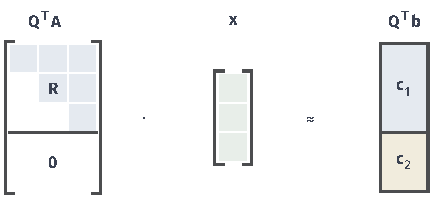
\includegraphics{figures/02-vectors-matrices-and-multivariate-calculus/03-linear-equations-and-optimization/tikz/learning-mechanisms/qr-residual-split.pdf}
  \caption{满列秩最小二乘的QR分解，示意$m=5,d=3$。正交变换后，矩阵上方的蓝色三角块为$\bm R$，下方为零；右端相应分成$\bm c_1$与$\bm c_2$。取$\bm R\hat{\bm x}=\bm c_1$后，残差$\bm r=\bm b-\bm A\hat{\bm x}$在变换后的坐标中上方为零，下方为$\bm c_2$，最小残差范数为$\lVert\bm c_2\rVert_2$。图中的近似号表示最小二乘匹配。}
  \label{fig:solver-qr-residual-split}
\end{figure}

\paragraph{满行秩的最小范数解}
同一种分解也能处理欠定方程。设$\bm A\in\mathbb R^{m\times d}$满行秩，$m<d$，求解目标改为第~\ref{sec:ls-select-among-solutions}节的最小范数精确解$\bm x_\star$。

最小范数解位于$\operatorname{range}(\bm A^\top)$中，需要的是这个子空间的标准正交基，所以对$\bm A^\top$而不是$\bm A$作薄QR分解
\begin{equation}
  \bm A^\top=\bm Q\bm R ,
 \label{eq:ls-qr-transpose-factorization}
\end{equation}
其中$\bm Q\in\mathbb R^{d\times m}$的列标准正交，$\bm R$为$m$阶可逆上三角矩阵。

于是
\[
  \bm A=\bm R^\top\bm Q^\top .
\]

把未知量写成$\bm x=\bm Q\bm y+\bm w$，其中$\bm Q^\top\bm w=\bm0$，代入方程得
\[
 \bm A\bm x=\bm R^\top\bm Q^\top\bm Q\bm y+\bm R^\top\bm Q^\top\bm w=\bm R^\top\bm y .
\]

方程只约束坐标$\bm y$，不约束$\bm w$。取$\bm w=\bm0$使范数最小（理由见算法分析），得
\begin{equation}
 \bm R^\top\bm y=\bm b,\qquad \bm x_\star=\bm Q\bm y .
 \label{eq:ls-qr-min-norm}
\end{equation}
第一式是下三角方程，按式~\eqref{eq:ls-forward-substitution}前代求出$\bm y$；第二式由坐标重建解。

\paragraph{只需应用正交因子}
两个分支都只用到$\bm Q^\top$或$\bm Q$对向量的作用，并不要求显式存出完整的$\bm Q$。后面三个小节提供三种计算方式：修正Gram--Schmidt直接算出$\bm Q_1$的各列，Householder方法保存一串反射向量，Givens方法保存一串旋转参数。它们都服务于上面同一个求解逻辑。

\subsection{算法实现}

输入是满列秩的$\bm A$与$\bm b$，输出是$\hat{\bm x}$；满行秩的欠定输入走本小节最后的转置QR分支。需要预先选定的只是因子的计算方法，三种选择见第~\ref{sec:ls-mgs}--\ref{sec:ls-givens}节。

算法由三个模块组成：QR分解给出$\bm R$并记录正交变换，变换右端求出$\bm c_1$，回代求出$\hat{\bm x}$。

下面仍用第~\ref{sec:ls-normal-equations-method}节的直线拟合数据逐步演示：
\[
  \bm A=\begin{bmatrix}1&0\\1&1\\1&2\end{bmatrix},\qquad \bm b=\begin{bmatrix}1\\2\\2\end{bmatrix}.
\]

\subsubsection{QR分解}
输入$\bm A$，输出$\bm R$以及正交因子或其变换记录。按第~\ref{sec:ls-mgs}、\ref{sec:ls-householder}、\ref{sec:ls-givens}节之一计算：修正Gram--Schmidt直接给出$\bm Q_1$的各列，Householder与Givens方法保存一串反射或旋转。

例中用修正Gram--Schmidt（逐步计算见第~\ref{sec:ls-mgs}节）得两个标准正交列
\[
 \bm q_1=\frac1{\sqrt3}\begin{bmatrix}1\\1\\1\end{bmatrix},\qquad
 \bm q_2=\frac1{\sqrt2}\begin{bmatrix}-1\\0\\1\end{bmatrix},
\]
以及三角因子
\[
 \bm R=\begin{bmatrix}\sqrt3&\sqrt3\\0&\sqrt2\end{bmatrix}.
\]

Householder与Givens方法给出的$\bm R$与它至多相差各行的符号。

若某个对角元$r_{j,j}=0$，说明$\bm A$秩亏，停止并改用第~\ref{sec:ls-svd-solve}节的SVD求解。

\subsubsection{变换右端}
输入正交因子与$\bm b$，输出$\bm c_1$。
\begin{enumerate}
 \item \textbf{计算$\bm c_1$。}按式~\eqref{eq:ls-qr-triangular-system}计算$\bm c_1=\bm Q_1^\top\bm b$。使用反射或旋转时，把它们按分解时的次序依次作用于$\bm b$，取结果的前$d$个分量；修正Gram--Schmidt中$\bm c_1$的计算次序在第~\ref{sec:ls-mgs}节说明。
 
 例中
 \[
  \bm c_1=\begin{bmatrix}\bm q_1^\top\bm b\\\bm q_2^\top\bm b\end{bmatrix}
  =\begin{bmatrix}5/\sqrt3\\1/\sqrt2\end{bmatrix}.
 \]

 \item \textbf{读出最小残差。}使用反射或旋转时，变换后右端的其余分量就是$\bm c_2$，$\lVert\bm c_2\rVert_2$即最小残差范数。
 
 例中若把$\bm Q_1$补齐为正交方阵，第三个标准正交向量及相应的右端分量为
 \[
  \bm q_3=\frac1{\sqrt6}\begin{bmatrix}1\\-2\\1\end{bmatrix},\qquad
  \bm c_2=\bm q_3^\top\bm b=-\frac1{\sqrt6},
 \]
 最小残差范数为$1/\sqrt6$。
\end{enumerate}

\subsubsection{回代}
输入$\bm R$与$\bm c_1$，输出$\hat{\bm x}$。
\begin{enumerate}
 \item \textbf{逐个求出$\hat x_i$。}根据式~\eqref{eq:ls-back-substitution}，对$i=d,\ldots,1$依次由式~\eqref{eq:ls-qr-triangular-system}得
 \[
  \hat x_i=\frac{(\bm c_1)_i-\sum_{j>i}r_{i,j}\hat x_j}{r_{i,i}} ;
 \]
 求出$\hat x_1$后结束。
 
 例中
 \[
  \hat x_2=\frac{1/\sqrt2}{\sqrt2}=\frac12,\qquad
  \hat x_1=\frac{\frac5{\sqrt3}-\sqrt3\cdot\frac12}{\sqrt3}=\frac76 .
 \]

 \item \textbf{输出并核验。}输出$\hat{\bm x}$，并以原始数据核验$\bm A^\top(\bm b-\bm A\hat{\bm x})=\bm0$。
 
 例中解与残差为
 \[
  \hat{\bm x}=\begin{bmatrix}7/6\\1/2\end{bmatrix},\qquad
  \bm r=\begin{bmatrix}-1/6\\1/3\\-1/6\end{bmatrix},
 \]
 并且$\bm A^\top\bm r=\bm0$。残差长度$1/\sqrt6$与上面读出的$\lvert\bm c_2\rvert$相同。
\end{enumerate}

例中的$\bm R$与$\bm c_1$恰是正规方程法中的$\bm L^\top$与前代结果$\bm y$：两条路线最后回代的是同一个三角方程，区别在于这里没有形成$\bm A^\top\bm A$。

\subsubsection{欠定情形：转置QR}
输入满行秩的$\bm A$（$m<d$）与$\bm b$，输出最小范数解$\bm x_\star$。
\begin{enumerate}
 \item \textbf{分解转置。}用上述任一种方法计算薄QR分解$\bm A^\top=\bm Q\bm R$。若$\bm R$出现零对角元，说明$\bm A$秩亏，停止并改用SVD求解。
 \item \textbf{前代。}根据式~\eqref{eq:ls-qr-min-norm}与式~\eqref{eq:ls-forward-substitution}，由下三角方程$\bm R^\top\bm y=\bm b$依次求出$y_1,\ldots,y_m$。
 \item \textbf{重建并核验。}计算$\bm x_\star=\bm Q\bm y$并输出，检查$\bm A\bm x_\star=\bm b$及$\bm x_\star\in\operatorname{range}(\bm A^\top)$。
\end{enumerate}

下例用一个欠定方程走一遍上述三步。

\begin{example}[转置QR给出最小范数解]
\label{ex:ls-qr-min-norm-run}
考虑下面的欠定方程：
\[
 \bm A=\begin{bmatrix}1&0&1\\0&1&1\end{bmatrix},\qquad
 \bm b=\begin{bmatrix}1\\2\end{bmatrix}.
\]
它有无穷多解。

$\bm A^\top$的两列为$(1,0,1)^\top$与$(0,1,1)^\top$。按修正Gram--Schmidt，先归一化第一列，并求出第二列沿它的分量：
\[
 \bm q_1=\frac1{\sqrt2}\begin{bmatrix}1\\0\\1\end{bmatrix},\qquad
 r_{1,2}=\frac1{\sqrt2}.
\]
扣除这一分量后归一化，得
\[
 \bm q_2=\frac1{\sqrt6}\begin{bmatrix}-1\\2\\1\end{bmatrix}.
\]
三角因子为
\[
 \bm R=\begin{bmatrix}\sqrt2&1/\sqrt2\\0&\sqrt{3/2}\end{bmatrix}.
\]
前代求解$\bm R^\top\bm y=\bm b$：
\[
 \begin{aligned}
 \sqrt2\,y_1&=1, & y_1&=\tfrac1{\sqrt2};\\
 \tfrac1{\sqrt2}y_1+\sqrt{3/2}\,y_2&=2, & y_2&=\sqrt{3/2} .
 \end{aligned}
\]
重建得
\[
 \bm x_\star=y_1\bm q_1+y_2\bm q_2
 =\frac12\begin{bmatrix}1\\0\\1\end{bmatrix}+\frac12\begin{bmatrix}-1\\2\\1\end{bmatrix}
 =\begin{bmatrix}0\\1\\1\end{bmatrix}.
\]
可以直接确认它的范数最小：本例全部解为$(1-t,2-t,t)^\top$，$t\in\mathbb R$，其范数平方为
\[
 (1-t)^2+(2-t)^2+t^2=3(t-1)^2+2 ,
\]
在$t=1$时最小，对应的正是$\bm x_\star$。
\end{example}

\subsection{算法分析}

\paragraph{正确性}
两个分支的正确性合写成下面的定理。

\begin{theorem}[QR给出最小二乘解与最小范数解]
\label{thm:ls-qr-least-squares}
设$\bm A\in\mathbb R^{m\times d}$，$\bm b\in\mathbb R^m$。
\begin{enumerate}
 \item 设$\bm A$满列秩，$\bm A=\bm Q\left[\begin{smallmatrix}\bm R\\\bm0\end{smallmatrix}\right]$，$\bm Q^\top\bm b=\left[\begin{smallmatrix}\bm c_1\\\bm c_2\end{smallmatrix}\right]$。则$\hat{\bm x}=\bm R^{-1}\bm c_1$是唯一的最小二乘解，最小残差范数为$\lVert\bm c_2\rVert_2$。
 \item 设$\bm A$满行秩，$\bm A^\top=\bm Q\bm R$为薄QR分解，$\bm R^\top\bm y=\bm b$。则$\bm x_\star=\bm Q\bm y$是$\bm A\bm x=\bm b$唯一的最小范数解。
\end{enumerate}
\end{theorem}
\begin{proof}
(1) 正交矩阵满足$\lVert\bm Q^\top\bm z\rVert_2^2=\bm z^\top\bm Q\bm Q^\top\bm z=\lVert\bm z\rVert_2^2$，所以式~\eqref{eq:ls-qr-residual-split}成立，其第二项与$\bm x$无关；$\bm R$可逆，第一项当且仅当$\bm x=\bm R^{-1}\bm c_1$时为零。

(2) 由$\bm Q^\top\bm Q=\bm I$，
\[
 \bm A\bm x_\star=\bm R^\top\bm Q^\top\bm Q\bm y=\bm R^\top\bm y=\bm b ,
\]
并且$\bm x_\star\in\operatorname{range}(\bm Q)=\operatorname{range}(\bm A^\top)=(\ker\bm A)^\perp$。任何其他解都与$\bm x_\star$相差$\ker\bm A$中的非零向量，即主要思想中的$\bm w\neq\bm0$，由勾股关系
\[
 \lVert\bm Q\bm y+\bm w\rVert_2^2=\lVert\bm y\rVert_2^2+\lVert\bm w\rVert_2^2 ,
\]
其范数更大。
\end{proof}

\paragraph{数值敏感度}
数值上要区分两个来源：最小二乘问题本身对数据的敏感度由问题决定（第~\ref{sec:ls-ls-regularization-sensitivity}节），计算QR因子时引入多少误差则取决于所用的正交化过程。三种实现在因子构造的工作量、数值正交性和残差核验方式上并不相同，下面分别说明。

\paragraph{秩亏情形}
秩亏时$\bm R$出现零对角元，不能照搬可逆$\bm R$的回代，最小范数最小二乘解按第~\ref{sec:ls-svd-solve}节用SVD求解。带列主元的QR能把线性无关的主元列排到前面，但只取主元变量回代、把其余原坐标置零，一般得到的是基本解，不能据此认定它是最小范数解。所以一般秩的情形本章统一使用SVD路线。

\subsection{修正Gram--Schmidt正交化}
\label{sec:ls-mgs}

本小节与后两小节计算同一组QR因子，思路分为两类。修正Gram--Schmidt从$\bm A$的各列出发，逐个造出标准正交方向，直接得到$\bm Q_1$的各列与$\bm R$。

Householder反射与Givens旋转则不写出$\bm Q$的列，而是对$\bm A$和$\bm b$依次施加正交变换，直到$\bm A$变成上三角形；正交因子只以这串变换的记录形式存在。正交变换保持长度，每一步之后$\lVert\bm A\bm x-\bm b\rVert_2$对任意$\bm x$都不变，所以变换结束时得到的正是式~\eqref{eq:ls-qr-triangular-system}的三角方程。

修正Gram--Schmidt的想法是一次确定一个新方向：一列减去它在已有方向上的分量，剩下的部分是这一列带来的新方向，归一化后就是下一个$\bm q_j$；减去的分量与剩下部分的长度记入$\bm R$。

\subsubsection{主要思想}
\term{修正Gram--Schmidt}（modified Gram--Schmidt）处理满列秩的$\bm A\in\mathbb R^{m\times d}$（$m\geq d$），目标是薄QR分解$\bm A=\bm Q_1\bm R$的因子。按列比较两边，第$k$列是
\begin{equation}
 \bm a_k=r_{1,k}\bm q_1+r_{2,k}\bm q_2+\cdots+r_{k,k}\bm q_k .
 \label{eq:ls-mgs-column-expansion}
\end{equation}
这个等式说明了$\bm R$中各元素的含义：$r_{i,k}$（$i<k$）是$\bm a_k$沿已有方向$\bm q_i$的分量，$r_{k,k}$是扣除这些分量后剩余部分的长度，$\bm q_k$是剩余部分的方向。$\bm R$是上三角矩阵，第$k$列只用到前$k$个方向，因此可以按列的次序逐个求出方向。

\paragraph{$d=2$的情况}
以$d=2$为例，两个等式是
\[
 \bm a_1=r_{1,1}\bm q_1,\qquad \bm a_2=r_{1,2}\bm q_1+r_{2,2}\bm q_2 .
\]
由第一式和$\lVert\bm q_1\rVert_2=1$，得
\[
 r_{1,1}=\lVert\bm a_1\rVert_2,\qquad \bm q_1=\bm a_1/r_{1,1} .
\]
第二式两边与$\bm q_1$作内积，由$\bm q_1^\top\bm q_2=0$得
\[
 r_{1,2}=\bm q_1^\top\bm a_2 ;
\]
移项后
\[
 r_{2,2}\bm q_2=\bm a_2-r_{1,2}\bm q_1 ,
\]
右边是$\bm a_2$扣除$\bm q_1$方向分量后的剩余向量，所以$r_{2,2}$是它的长度，$\bm q_2$是它的方向。

\paragraph{一般情况}
列数更多时，每一列要扣除的已有方向也更多。记$\bm v_k$为第$k$列的当前剩余向量，即第$k$列中尚未由已有方向表示的部分，开始时$\bm v_k=\bm a_k$。修正形式的做法是：每得到一个新方向，就立刻从所有尚未处理的列中扣除这一方向上的分量。于是轮到第$j$列时，$\bm v_j$已经扣除了$\bm q_1,\ldots,\bm q_{j-1}$方向的分量，剩下的只有新方向，由第$j$列的等式得
\begin{equation}
 r_{j,j}=\lVert\bm v_j\rVert_2,\qquad \bm q_j=\bm v_j/r_{j,j};
 \label{eq:ls-mgs-normalize}
\end{equation}
随后对每个$k>j$扣除$\bm q_j$方向的分量：
\begin{equation}
 r_{j,k}=\bm q_j^\top\bm v_k,\qquad \bm v_k\leftarrow\bm v_k-r_{j,k}\bm q_j .
 \label{eq:ls-mgs-update}
\end{equation}

与第~\ref{chap:inner-product-spaces}章的Gram--Schmidt正交化相比，它只差一处：投影系数用已经扣除了前面分量的当前剩余向量计算，而不是都用原始列$\bm a_k$。

精确算术中两种算法给出同一组因子。有限精度下，算出的$\bm q_2$与$\bm q_1$并不严格正交。原来的做法用$\bm q_2^\top\bm a_k$计算系数；若$\bm a_k$在$\bm q_1$方向上的分量很大，$\bm q_2$对正交性的微小偏离会与这一大分量相乘，混入$r_{2,k}$。

修正形式所用的$\bm v_k$已经扣除了$\bm q_1$方向的分量，同样的偏离只与很小的残留分量相乘。这只说明误差的来源，正交性的检查方法见本小节的算法分析。

求解还需要$\bm c_1=\bm Q_1^\top\bm b$。把右端当作额外的一列，按同样的次序扣除：令$\bm s=\bm b$，对$i=1,\ldots,d$依次计算
\begin{equation}
 c_i=\bm q_i^\top\bm s,\qquad \bm s\leftarrow\bm s-c_i\bm q_i .
 \label{eq:ls-mgs-rhs}
\end{equation}
每次扣除取走$\bm b$在一个方向上能由$\bm A$的列表示的部分，$c_i$记录取走的量。全部扣除后，$\bm s$就是$\bm b$减去它在列空间上的投影，即最小二乘残差；$\bm c_1=(c_1,\ldots,c_d)^\top$交给式~\eqref{eq:ls-qr-triangular-system}回代。

\subsubsection{算法实现}
输入是满列秩的$\bm A$与$\bm b$，输出是$\hat{\bm x}$，没有需要预先选定的规则。算法逐列进行，用$j$记当前处理的列，维护剩余向量$\bm v_1,\ldots,\bm v_d$、$\bm R$的已算元素和右端的剩余向量$\bm s$；全部列处理完后回代。

下面仍用直线拟合数据逐步演示：
\[
  \bm A=\begin{bmatrix}1&0\\1&1\\1&2\end{bmatrix},\qquad \bm b=\begin{bmatrix}1\\2\\2\end{bmatrix}.
\]

\begin{enumerate}
 \item \textbf{初始化。}令$\bm v_k=\bm a_k$（$k=1,\ldots,d$），$\bm R=\bm0$，$\bm s=\bm b$，$j=1$。

 例中两列的剩余向量为
 \[
  \bm v_1=\begin{bmatrix}1\\1\\1\end{bmatrix},\qquad
  \bm v_2=\begin{bmatrix}0\\1\\2\end{bmatrix},
 \]
 右端的剩余向量为$\bm s=(1,2,2)^\top$。

 \item \textbf{归一化当前列。}此时$\bm v_j$已经扣除了全部已有方向的分量，剩下的是第$j$列带来的新方向。根据式~\eqref{eq:ls-mgs-normalize}算出它的长度$r_{j,j}$与方向$\bm q_j$。若$r_{j,j}=0$，说明第$j$列落在前面各列的张成中，满列秩的前提不成立，停止并改用SVD求解。

 例中$j=1$，
 \[
  r_{1,1}=\lVert\bm v_1\rVert_2=\sqrt3,\qquad
  \bm q_1=\frac1{\sqrt3}\begin{bmatrix}1\\1\\1\end{bmatrix}.
 \]

 \item \textbf{扣除新方向。}新方向一经确定，就从后面各列和右端中扣除，后续步骤面对的都是已经扣除这一方向的向量。根据式~\eqref{eq:ls-mgs-update}，对每个$k>j$算出$r_{j,k}$并更新$\bm v_k$；再根据式~\eqref{eq:ls-mgs-rhs}算出$c_j$并更新$\bm s$。

 例中对第二列，先求分量$r_{1,2}=\bm q_1^\top\bm v_2=\sqrt3$，再扣除：
 \[
  \bm v_2\leftarrow\begin{bmatrix}0\\1\\2\end{bmatrix}-\begin{bmatrix}1\\1\\1\end{bmatrix}=\begin{bmatrix}-1\\0\\1\end{bmatrix}.
 \]
 对右端，先求$c_1=\bm q_1^\top\bm s=5/\sqrt3$，再扣除：
 \[
  \bm s\leftarrow\begin{bmatrix}1\\2\\2\end{bmatrix}-\frac53\begin{bmatrix}1\\1\\1\end{bmatrix}=\begin{bmatrix}-2/3\\1/3\\1/3\end{bmatrix}.
 \]

 在直线拟合中，扣除全一方向$\bm q_1$就是减去平均值：$\bm v_2$是横坐标$0,1,2$减去均值$1$，$\bm s$是$\bm b$减去均值$5/3$。

 \item \textbf{判断是否结束。}若$j<d$，令$j\leftarrow j+1$，回到第2步；否则结束。

 例中$j=1<2$，令$j=2$。第2步得
 \[
  r_{2,2}=\lVert\bm v_2\rVert_2=\sqrt2,\qquad
  \bm q_2=\frac1{\sqrt2}\begin{bmatrix}-1\\0\\1\end{bmatrix};
 \]
 第3步右侧已没有待处理的列，只处理右端：先求$c_2=\bm q_2^\top\bm s=1/\sqrt2$，再扣除，
 \[
  \bm s\leftarrow\begin{bmatrix}-2/3\\1/3\\1/3\end{bmatrix}-\frac12\begin{bmatrix}-1\\0\\1\end{bmatrix}=\begin{bmatrix}-1/6\\1/3\\-1/6\end{bmatrix}.
 \]

 这时$j=d$，结束，得
 \[
  \bm R=\begin{bmatrix}\sqrt3&\sqrt3\\0&\sqrt2\end{bmatrix},\qquad
  \bm c_1=\begin{bmatrix}5/\sqrt3\\1/\sqrt2\end{bmatrix}.
 \]
 可以核验
 \[
  \bm q_1^\top\bm q_2=0,\qquad
  \sqrt3\,\bm q_1+\sqrt2\,\bm q_2=\begin{bmatrix}0\\1\\2\end{bmatrix}=\bm a_2 .
 \]
 第二式正是$\bm R$第二列的含义：$\bm a_2$沿$\bm q_1$的分量为$\sqrt3$，剩余部分长度为$\sqrt2$。

 最后剩下的$\bm s$正是直线拟合的残差，长度为$1/\sqrt6$。

 \item \textbf{回代。}按式~\eqref{eq:ls-qr-triangular-system}回代求解$\bm R\hat{\bm x}=\bm c_1$，输出$\hat{\bm x}$。

 例中的$\bm R$与$\bm c_1$与第~\ref{sec:ls-qr-method}节算法实现所用的相同，回代得
 \[
  \hat{\bm x}=\begin{bmatrix}7/6\\1/2\end{bmatrix}.
 \]
\end{enumerate}

$\bm Q_1$、$\bm R$和剩余向量都只是内部状态。按列组织时也可以对第$j$列依次扣除$\bm q_1,\ldots,\bm q_{j-1}$方向的分量，每次内积都用刚更新过的剩余向量；它对每一列执行的运算与上面相同，只是循环次序不同。

有限精度下若发现某列扣除后明显变短，可以对它再正交化一遍，并把第二遍得到的投影系数加到已累计的$r_{i,j}$上，使$\bm A=\bm Q_1\bm R$仍然成立。右端也要按式~\eqref{eq:ls-mgs-rhs}逐次扣除：有限精度下$\bm Q_1$的列不完全正交，不宜把它换成另算$\bm Q_1^\top\bm b$。

\subsubsection{算法分析}
先看精确算术中的不变关系。式~\eqref{eq:ls-mgs-update}更新后，
\[
  \bm q_j^\top\bm v_k=\bm q_j^\top\bm v_k-r_{j,k}=0 ,
\]
即$\bm v_k$与$\bm q_j$正交。

扣除的是$\bm q_j$方向的分量，而$\bm q_j$与$\bm q_1,\ldots,\bm q_{j-1}$正交，所以$\bm v_k$仍与它们正交。因此第$j$步归一化的$\bm v_j$与此前全部方向正交，各$\bm q_i$两两正交。

同时，每次扣除都把分量记入$\bm R$，所以整个过程维持
\begin{equation}
 \bm a_k=\sum_{i\leq j}r_{i,k}\bm q_i+\bm v_k\qquad(k>j),
 \label{eq:ls-mgs-invariant}
\end{equation}
即原始列始终等于已提取的分量加上当前剩余向量。

全部列处理完毕时剩余部分已归入各$\bm q_k$，得到
\[
  \bm A=\bm Q_1\bm R .
\]

又因各$\bm q_i$两两正交，对剩余向量和对原始列计算的内积相同：
\begin{equation}
  \bm q_i^\top\Bigl(\bm a_j-\sum_{k<i}r_{k,j}\bm q_k\Bigr)=\bm q_i^\top\bm a_j .
 \label{eq:ls-mgs-cgs-equivalence}
\end{equation}

所以修正形式给出与原来相同的QR分解；同样的论证说明式~\eqref{eq:ls-mgs-rhs}给出$c_i=\bm q_i^\top\bm b$。由定理~\ref{thm:ls-qr-least-squares}，回代所得即最小二乘解。

有限精度下，近相关的列扣除旧方向后剩余向量很短，其中舍入误差的相对影响被放大，算出的$\bm q_j$会偏离正交，这就是再正交化要处理的情形。

检查结果时用$\lVert\bm Q_1^\top\bm Q_1-\bm I\rVert$衡量正交性，用$\lVert\bm A-\bm Q_1\bm R\rVert$衡量重构质量，二者要分开看：后者小并不保证前者小。正交性损失的程度与$\bm A$的条件数有关，具体说明见第~\ref{sec:ls-numerical-stability}节。主要工作约为$2md^2$次运算。

\subsection{Householder反射}
\label{sec:ls-householder}

\subsubsection{主要思想}
Householder方法不构造$\bm Q_1$的列，而是逐列把$\bm A$化成上三角形。第$k$步用一个镜面反射，把第$k$列从对角元往下的部分变成坐标轴方向，于是对角元下方的元素全部变为零；同一个反射也作用于其余各列和$\bm b$。

$d$次反射之后得到$\bm R$与变换后的右端，正交因子就是这一串反射的乘积：
\begin{equation}
  \bm Q^\top=\bm H_d\cdots\bm H_1
 \label{eq:ls-householder-qt}
\end{equation}
使$\bm H_d\cdots\bm H_1\bm A$成为上三角矩阵。

第$k$步的核心问题是：给定一个列段$\bm y\neq\bm0$，怎样构造正交矩阵把它映到第一个坐标轴上。

正交变换不改变长度，$\bm y$只能被送到同样长的轴向量$\alpha\bm e_1$，$\lvert\alpha\rvert=\lVert\bm y\rVert_2$。在平面上可以直接找到这样的变换：$\bm y$与$\alpha\bm e_1$到原点的距离相同，原点落在两点连线的垂直平分线上；以这条垂直平分线为镜子作反射，$\bm y$恰好落到$\alpha\bm e_1$。镜子与两点之差$\bm y-\alpha\bm e_1$垂直，所以镜子的法向就是$\bm v=\bm y-\alpha\bm e_1$。高维时镜子换成以$\bm v$为法向的超平面。

这种反射称为\term{Householder反射}（Householder reflection），写作
\begin{equation}
  \bm H=\bm I-2\bm v\bm v^\top/(\bm v^\top\bm v)
 \label{eq:ls-householder-reflector}
\end{equation}
它把$\bm v$方向的分量变号，保持与$\bm v$正交的分量不变，是关于以$\bm v$为法向的超平面的镜面反射。它对称且正交，所以只需选好$\bm v$，如图~\ref{fig:ls-householder-reflection}所示。

\begin{figure}[htbp]
  \centering
  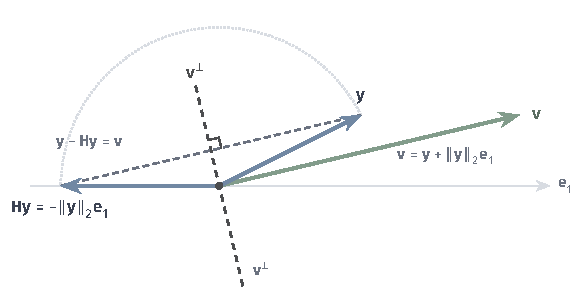
\includegraphics[width=98.94mm]{figures/01-basic-mathematics/03-vectors-matrices-and-multivariate-functions/tikz/c5-householder-reflection/figure.pdf}
  \caption{Householder反射的几何。取$\bm y=(2,1)^\top$，按式~\eqref{eq:ls-householder}令$\bm v=\bm y+\sqrt5\,\bm e_1$。反射超平面$\bm v^\perp$是$\bm y$与$\bm H\bm y=-\sqrt5\,\bm e_1$连线的垂直平分线，两者之差恰为$\bm v$；点线圆弧表示反射保持长度。解析式构造。}
  \label{fig:ls-householder-reflection}
\end{figure}

几何构造给出的$\bm v$也可以从代数上确认。要求的等式是$\bm H\bm y=\alpha\bm e_1$。正交变换保持长度，所以
\[
 \alpha^2=\bm y^\top\bm y,\qquad \alpha=\pm\lVert\bm y\rVert_2 .
\]
展开左边，
\[
 \bm H\bm y=\bm y-\frac{2\bm v^\top\bm y}{\bm v^\top\bm v}\,\bm v=\alpha\bm e_1 ,
\]
所以$\bm y-\alpha\bm e_1$必须是$\bm v$的倍数。反射只依赖$\bm v$的方向，于是取
\[
 \bm v=\bm y-\alpha\bm e_1 ;
\]
这一选择确实使系数$2\bm v^\top\bm y/(\bm v^\top\bm v)$等于$1$，从而
\[
 \bm H\bm y=\bm y-\bm v=\alpha\bm e_1 ,
\]
验证见本小节算法分析中的引理。

$\alpha$的两个符号对应坐标轴上的两个候选目标$\pm\lVert\bm y\rVert_2\bm e_1$，精确算术中都可以用。若$\bm y$本来就接近其中一个目标，它与该目标几乎重合，二者之差$\bm v$很短，镜子的朝向难以准确算出；所以实际选择与$\bm y$的首分量异号、离$\bm y$较远的那个目标。具体地取$\alpha=-s\lVert\bm y\rVert_2$，其中$y_1\geq0$时$s=1$、$y_1<0$时$s=-1$，即
\begin{equation}
 \bm v=\bm y+s\lVert\bm y\rVert_2\bm e_1,\qquad
 \bm H=\bm I-\frac{2\bm v\bm v^\top}{\bm v^\top\bm v},
 \label{eq:ls-householder}
\end{equation}
这样$\bm v$的首分量$v_1=y_1+s\lVert\bm y\rVert_2$是两个同号数相加；数值上的理由见算法分析。

作用于其他向量时不形成稠密的$\bm H$：令$\tau=2/(\bm v^\top\bm v)$，则对任意向量$\bm z$都有
\begin{equation}
 \bm H\bm z=\bm z-\tau\,(\bm v^\top\bm z)\,\bm v ,
 \label{eq:ls-householder-apply}
\end{equation}
即减去$\bm z$在$\bm v$方向上分量的两倍，只需一次内积和一次向量更新。

第$k$步的反射只作用于第$k$至$m$行，嵌入$m$阶后为
\begin{equation}
 \bm H_k=\operatorname{diag}(\bm I_{k-1},\bm H) .
 \label{eq:ls-householder-embedding}
\end{equation}
前$k-1$行已经是$\bm R$的确定部分，不再改动；前$k-1$列在第$k$至$m$行上的零也保持为零（见算法分析），所以逐列进行时，已经造出的零不会被后面的反射破坏。

\subsubsection{算法实现}
输入是满列秩的$\bm A\in\mathbb R^{m\times d}$（$m\geq d$）与$\bm b$，输出是$\hat{\bm x}$。需要预先选定的规则是式~\eqref{eq:ls-householder}中符号$s$的取法，并保持原列顺序，不选列主元。

算法逐列进行，用$k$记当前处理的列，维护工作矩阵$\bm F$与工作右端$\bm c$；三角化结束后回代。仍用直线拟合数据演示，每一列处理完后给出$\bm F$与$\bm c$的当前值。
\begin{enumerate}
 \item \textbf{初始化。}令$\bm F=\bm A$，$\bm c=\bm b$，$k=1$。

 例中
 \[
  \bm F=\begin{bmatrix}1&0\\1&1\\1&2\end{bmatrix},\qquad
  \bm c=\begin{bmatrix}1\\2\\2\end{bmatrix}.
 \]

 \item \textbf{构造反射。}取当前列段$\bm y=\bm F_{k:m,k}$，即第$k$列中从对角元往下、尚未处理的部分，根据式~\eqref{eq:ls-householder}构造$\bm v$与$\tau=2/(\bm v^\top\bm v)$，保存这一反射记录。
 
 若$\bm y=\bm0$，说明第$k$列落在前面各列的张成中，满列秩的前提不成立，停止并改用SVD求解；若$\bm y$在第一个分量以下已经全为零，可以取恒等变换，跳过第3步。

 例中$k=1$，$\bm y=(1,1,1)^\top$，$\lVert\bm y\rVert_2=\sqrt3$，$y_1>0$，取$s=1$，于是
 \[
  \bm v=\begin{bmatrix}1+\sqrt3\\1\\1\end{bmatrix},\qquad \bm v^\top\bm v=6+2\sqrt3,\qquad \tau=\frac1{3+\sqrt3}.
 \]

 \item \textbf{作用于剩余子块与右端。}整个问题必须经受同一个正交变换，残差长度才保持不变，所以反射不仅作用于第$k$列，也作用于其余各列和右端。
 
 根据式~\eqref{eq:ls-householder-apply}，把这个反射作用于剩余子块$\bm F_{k:m,k:d}$的各列和右端$\bm c_{k:m}$；第$k$列不必计算，直接成为$(-s\lVert\bm y\rVert_2,0,\ldots,0)^\top$。

 例中第一列变为$(-\sqrt3,0,0)^\top$；对第二列$\bm z=(0,1,2)^\top$与右端$\bm c$分别算出
 \[
  \begin{aligned}
  &\text{第二列：}&& \bm v^\top\bm z=3,\quad \tau\,\bm v^\top\bm z=\tfrac{3-\sqrt3}2;\\
  &\text{右端：}&& \bm v^\top\bm c=5+\sqrt3,\quad \tau\,\bm v^\top\bm c=2-\tfrac{\sqrt3}3 .
  \end{aligned}
 \]
 各自减去相应倍数的$\bm v$，得
 \[
  \bm F=\begin{bmatrix}-\sqrt3&-\sqrt3\\0&\frac{\sqrt3-1}2\\[2pt]0&\frac{\sqrt3+1}2\end{bmatrix},\qquad
  \bm c=\begin{bmatrix}-5/\sqrt3\\1/\sqrt3\\1/\sqrt3\end{bmatrix}.
 \]
 第一列已经成为坐标轴方向，第一行从此确定，后面只处理第2、3行。两列与右端的长度平方仍为$3$、$5$、$9$，与变换前相同，这是反射保持长度的直接检验。

 \item \textbf{判断是否结束。}若$k<d$，令$k\leftarrow k+1$，回到第2步；否则结束。

 例中$k=1<2$，令$k=2$。第2步取第二列的后两个元素
 \[
  \bm y=\begin{bmatrix}\frac{\sqrt3-1}2\\[2pt]\frac{\sqrt3+1}2\end{bmatrix},\qquad
  \lVert\bm y\rVert_2=\sqrt2,\qquad s=1,
 \]
 由此构造反射向量
 \[
  \bm v=\begin{bmatrix}\frac{\sqrt3-1}2+\sqrt2\\[2pt]\frac{\sqrt3+1}2\end{bmatrix}.
 \]
 第3步只作用于后两行，第二列的这一段与右端的后两个分量分别变为
 \[
  \begin{bmatrix}-\sqrt2\\0\end{bmatrix},\qquad
  \begin{bmatrix}-1/\sqrt2\\-1/\sqrt6\end{bmatrix}.
 \]
 这一段也成为坐标轴方向，第一列的零与第一行都没有改动。

 这时$k=d$，结束，得
 \[
  \bm F=\begin{bmatrix}-\sqrt3&-\sqrt3\\0&-\sqrt2\\0&0\end{bmatrix},\qquad
  \bm c=\begin{bmatrix}-5/\sqrt3\\-1/\sqrt2\\-1/\sqrt6\end{bmatrix}.
 \]

 \item \textbf{回代。}取$\bm R=\bm F_{1:d,1:d}$，检查对角元非零，再按式~\eqref{eq:ls-qr-triangular-system}回代求解$\bm R\hat{\bm x}=\bm c_{1:d}$，输出$\hat{\bm x}$；$\bm F$的后$m-d$行为零，$\bm c_{d+1:m}$是任何$\bm x$都无法拟合的部分，$\lVert\bm c_{d+1:m}\rVert_2$是最小残差范数。

 例中
 \[
  \hat x_2=\frac{-1/\sqrt2}{-\sqrt2}=\frac12,\qquad
  \hat x_1=\frac{-\frac5{\sqrt3}+\sqrt3\cdot\frac12}{-\sqrt3}=\frac53-\frac12=\frac76,
 \]
 $\lvert c_3\rvert=1/\sqrt6$正是最小残差范数。
\end{enumerate}

例中的$\bm R$与正规方程法的Cholesky因子$\bm L^\top$只差各行的符号。对角元为负不影响求解；若要统一成正对角，须把$\bm R$的相应行与变换后右端的相应分量同时变号。

\subsubsection{算法分析}
单步消元的依据是下面的引理。

\begin{lemma}[Householder反射]
\label{lem:ls-householder-reflection}
设$\bm y\neq\bm0$，$\bm v$与$\bm H$由式~\eqref{eq:ls-householder}给出。则$\bm H$对称正交，且$\bm H\bm y=-s\lVert\bm y\rVert_2\bm e_1$。
\end{lemma}
\begin{proof}
$\bm H$显然对称；
\[
 \bm H^2=\bm I-\frac{4\bm v\bm v^\top}{\bm v^\top\bm v}+\frac{4\bm v(\bm v^\top\bm v)\bm v^\top}{(\bm v^\top\bm v)^2}=\bm I ,
\]
所以$\bm H^\top\bm H=\bm I$。由$s^2=1$与$sy_1=\lvert y_1\rvert$，
\[
 \bm v^\top\bm v=2\lVert\bm y\rVert_2^2+2\lVert\bm y\rVert_2\lvert y_1\rvert=2\bm v^\top\bm y>0,
\]
于是$\bm H\bm y=\bm y-\bm v=-s\lVert\bm y\rVert_2\bm e_1$。
\end{proof}

每个$\bm H_k$只作用于第$k$至$m$行；前$k-1$列在这些行上已经是零，反射后仍为零。所以旧的零结构保持不变，$d$步后$\bm F=\bm H_d\cdots\bm H_1\bm A$是上三角矩阵，$\bm c=\bm H_d\cdots\bm H_1\bm b$。这正是取$\bm Q^\top=\bm H_d\cdots\bm H_1$的QR分解，由定理~\ref{thm:ls-qr-least-squares}，回代所得即最小二乘解。

符号的选择影响数值精度。$\bm v$的首分量是$y_1-\alpha$；若$\alpha$与$y_1$同号且$\bm y$接近$\bm e_1$方向，这是两个相近数相减，会严重相消。取$\alpha=-s\lVert\bm y\rVert_2$使$v_1$成为两个同号数相加，避免了这种相消。

Householder QR后向稳定（第~\ref{sec:ls-numerical-stability}节），算出的$\bm Q$在舍入误差范围内保持正交，主要工作约为$2md^2-\tfrac23d^3$次运算。列主元可以辅助辨认近相关的列，但秩亏时的最小范数选择仍回到第~\ref{sec:ls-svd-solve}节。

\subsection{Givens旋转}
\label{sec:ls-givens}

Givens方法同样用正交变换把$\bm A$和$\bm b$化成上三角形，但每次只消去一个元素：在两行构成的平面内作一次旋转，把其中一个元素转为零。

Householder反射一步处理一整列，Givens旋转一步只改动两行，其余各行原样保留。当对角线以下只有少数非零元，或者要在已有的$\bm R$上补入一条新观测时，只需对少数几对行作旋转，这种局部性就带来实际的节省。

\subsubsection{主要思想}
\term{Givens旋转}（Givens rotation）在两个坐标构成的平面内旋转，其余坐标不变；每次只混合两行，消去其中一个元素。所求的正交因子$\bm Q^\top$是一串这样的旋转之积。图~\ref{fig:ls-givens-householder-elimination}把旋转与反射并置。

\begin{figure*}[htbp]
  \centering
  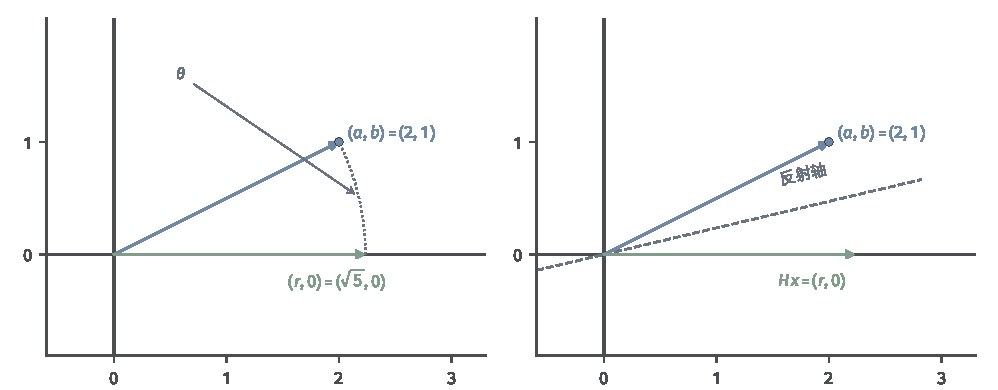
\includegraphics[width=168.998mm]{figures/00-shared/mathematical-preliminaries-upper/02-linear-spaces/matplotlib/ls-givens-householder-elimination/ls-givens-householder-elimination.pdf}
  \caption{两种初等正交消元。左：Givens旋转把$(a,b)=(2,1)^\top$沿圆弧旋到
  $(r,0)^\top$，$r=\sqrt5$，旋转角$\theta=\arctan(1/2)$；右：Householder反射沿角平分线
  把同一向量映到$(r,0)^\top$。两者都是正交变换，保持长度，区别在旋转（行列式$+1$）与
  反射（对称正交）。图中的反射取与式~\eqref{eq:ls-householder}相反的符号，精确算术中两种选择都可以。解析式教学构造。}
  \label{fig:ls-givens-householder-elimination}
\end{figure*}

先看二维问题：给定$(\alpha,\beta)^\top\neq\bm0$，求旋转$\bm G=\left[\begin{smallmatrix}c&s\\-s&c\end{smallmatrix}\right]$使$\bm G(\alpha,\beta)^\top=(\rho,0)^\top$。几何上，设向量$(\alpha,\beta)^\top$与第一坐标轴的夹角为$\theta$，把它顺时针转过$\theta$就落到第一坐标轴上；旋转保持长度，所以落点是$(\rho,0)^\top$，$\rho$是向量的长度。这个旋转矩阵的元素是$c=\cos\theta$与$s=\sin\theta$，而夹角的余弦与正弦就是$\alpha/\rho$与$\beta/\rho$，所以不必求出角度本身。

代数上逐个分量写出，连同旋转的条件，要求
\[
 c\alpha+s\beta=\rho,\qquad -s\alpha+c\beta=0,\qquad c^2+s^2=1 .
\]
由第二式，$(c,s)$与$(\alpha,\beta)$平行；由第三式归一化并取$\rho>0$，得
\[
 c=\frac\alpha\rho,\qquad s=\frac\beta\rho ;
\]
代入第一式得
\[
 \rho=\frac{\alpha^2+\beta^2}{\rho} .
\]
合起来，
\begin{equation}
 \begin{gathered}
 \rho=\sqrt{\alpha^2+\beta^2},\qquad c=\alpha/\rho,\qquad s=\beta/\rho,\\
 \bm G=\begin{bmatrix}c&s\\-s&c\end{bmatrix}.
 \end{gathered}
 \label{eq:ls-givens}
\end{equation}
这里的$s$与Householder反射中的符号无关。$\alpha=\beta=0$时取恒等变换。

对矩阵的两行$p,q$同时作用时，新的两行是
\begin{equation}
 \begin{aligned}
 \text{第}p\text{行}&\leftarrow c\cdot(\text{第}p\text{行})+s\cdot(\text{第}q\text{行}),\\
 \text{第}q\text{行}&\leftarrow -s\cdot(\text{第}p\text{行})+c\cdot(\text{第}q\text{行}),
 \end{aligned}
 \label{eq:ls-givens-rows}
\end{equation}
右端的两个分量也按同样的方式更新。参数$c,s$由两行在某一列的元素确定，使第$q$行在该列变为零、第$p$行在该列变为$\rho$；同一个旋转作用于两行的其余元素和右端，保证整个问题经受同一个正交变换。

三角化时逐列进行，在每一列中自下而上用相邻两行消去对角线下方的元素。每次旋转把下一行在这一列的元素并入上一行，非零部分就逐行向上汇集，最后集中到对角元上，对角元的绝对值等于这一列对角元及其下方各元素组成的列段的长度。被消零的行不再参与本列后面的旋转，前面各列的零也不受影响，理由见本小节的算法分析。

\subsubsection{算法实现}
输入是满列秩的$\bm A\in\mathbb R^{m\times d}$（$m\geq d$）和$\bm b$，输出是$\hat{\bm x}$。需要预先选定的规则是消元次序：按$k=1,\ldots,d$处理各列，在第$k$列中按$i=m,m-1,\ldots,k+1$自下而上消去$f_{i,k}$，每次使用相邻的第$i-1$、$i$两行。算法维护工作矩阵$\bm F$与工作右端$\bm t$，右端记作$\bm t$是为了不与旋转参数$c$混淆。下面先给出三角化与回代，再给出新增一条观测时的更新。仍用直线拟合数据演示，把右端写在增广列中。

\paragraph{三角化与回代}
\begin{enumerate}
 \item \textbf{初始化。}令$\bm F=\bm A$，$\bm t=\bm b$，$k=1$，$i=m$。

 例中
 \[
  [\bm F\mid\bm t]=\left[\begin{array}{cc|c}1&0&1\\1&1&2\\1&2&2\end{array}\right].
 \]

 \item \textbf{构造旋转。}若$f_{i,k}=0$，这个位置已经是零，直接转到第4步；否则令$\alpha=f_{i-1,k}$为上一行的元素、$\beta=f_{i,k}$为要消去的元素，根据式~\eqref{eq:ls-givens}计算$\rho,c,s$。为避免上溢或下溢，平方和可以先除以$\max(\lvert\alpha\rvert,\lvert\beta\rvert)$，开方后再恢复尺度，许多程序库以hypot函数提供这一计算。

 例中$k=1$、$i=3$，
 \[
  \alpha=\beta=1,\qquad \rho=\sqrt2,\qquad c=s=\frac1{\sqrt2}.
 \]

 \item \textbf{旋转两行。}根据式~\eqref{eq:ls-givens-rows}，用同一个$\bm G$作用于$\bm F$的第$i-1$、$i$两行在第$k$列及以后的部分，并同步变换$(t_{i-1},t_i)^\top$，保存这次旋转的参数。第$k$列以前的部分在两行中都是零，旋转后仍为零，不必计算。两式必须读取同一对旧行，计算时先用临时量保存旧值；若先覆盖第$i-1$行再用它计算第$i$行，结果就不再是旋转。

 例中第$2$、$3$两行变为
 \[
  \bigl(\sqrt2,\tfrac3{\sqrt2}\bigm|2\sqrt2\bigr),\qquad
  \bigl(0,\tfrac1{\sqrt2}\bigm|0\bigr).
 \]
 第3行的第一个元素已经消去，它的值并入第2行，第2行的首元素变为两个$1$组成的向量的长度$\sqrt2$。

 \item \textbf{判断是否结束。}若$i>k+1$，令$i\leftarrow i-1$，回到第2步；否则第$k$列已经完成，若$k<d$，令$k\leftarrow k+1$、$i=m$，回到第2步；若$k=d$，三角化结束。

 例中先令$i=2$，用第$1$、$2$行消去$f_{2,1}=\sqrt2$：
 \[
  \alpha=1,\qquad \beta=\sqrt2,\qquad \rho=\sqrt3,\qquad c=\frac1{\sqrt3},\qquad s=\sqrt{2/3},
 \]
 两行变为
 \[
  \bigl(\sqrt3,\sqrt3\bigm|\tfrac5{\sqrt3}\bigr),\qquad
  \bigl(0,\sqrt{3/2}\bigm|\sqrt{2/3}\bigr).
 \]
 第一列完成：三个$1$逐行向上汇集，对角元成为$\sqrt3=\lVert\bm a_1\rVert_2$。

 再令$k=2$、$i=3$，用第$2$、$3$行消去$f_{3,2}=1/\sqrt2$：
 \[
  \alpha=\sqrt{3/2},\qquad \beta=\frac1{\sqrt2},\qquad \rho=\sqrt2,\qquad c=\frac{\sqrt3}2,\qquad s=\frac12,
 \]
 两行变为
 \[
  \bigl(0,\sqrt2\bigm|\tfrac1{\sqrt2}\bigr),\qquad
  \bigl(0,0\bigm|-\tfrac1{\sqrt6}\bigr).
 \]
 这时$k=d$，结束，得
 \[
  [\bm F\mid\bm t]=\left[\begin{array}{cc|c}\sqrt3&\sqrt3&5/\sqrt3\\0&\sqrt2&1/\sqrt2\\0&0&-1/\sqrt6\end{array}\right].
 \]

 \item \textbf{回代。}取$\bm R=\bm F_{1:d,1:d}$，按式~\eqref{eq:ls-qr-triangular-system}回代求解$\bm R\hat{\bm x}=\bm t_{1:d}$，输出$\hat{\bm x}$，并用原始数据检查残差。

 例中$\bm R$恰为正规方程法的Cholesky因子$\bm L^\top$，$\bm t_{1:2}$恰为那里的前代结果$\bm y$，回代得
 \[
  \hat{\bm x}=\begin{bmatrix}7/6\\1/2\end{bmatrix},\qquad
  \lvert t_3\rvert=\frac1{\sqrt6},
 \]
 后者为最小残差范数。
\end{enumerate}

\paragraph{新增观测的更新}
局部消元的好处在新增观测时最明显。设已经有$d$阶上三角的$\bm R$和$\bm c_1$，新到一条观测行$\bm w^\top$及其右端$\eta$，要求加入这条观测后的最小二乘解，而不重新处理旧的观测行。

由式~\eqref{eq:ls-qr-residual-split}，旧观测对$\bm x$的全部约束都已经由$\lVert\bm R\bm x-\bm c_1\rVert_2^2$表达，$\lVert\bm c_2\rVert_2^2$只是与$\bm x$无关的常数。所以只需把新行排在$[\bm R\mid\bm c_1]$下方，再用旋转把它逐个元素并入$\bm R$。
\begin{enumerate}
 \item \textbf{排列。}把$(\bm w^\top\mid\eta)$排在$[\bm R\mid\bm c_1]$下方。例中在直线拟合的三个点之外新增点$(3,3)$，即$\bm w=(1,3)^\top$、$\eta=3$，上方是三角化得到的$\bm R$与$\bm c_1$，排列后为
 \[
  \left[\begin{array}{cc|c}\sqrt3&\sqrt3&5/\sqrt3\\0&\sqrt2&1/\sqrt2\\\hline1&3&3\end{array}\right].
 \]

 \item \textbf{逐个消去新行的元素。}对$k=1,\ldots,d$，取$\alpha=r_{k,k}$、$\beta$为新行当前的第$k$个元素，按式~\eqref{eq:ls-givens}与式~\eqref{eq:ls-givens-rows}旋转$\bm R$的第$k$行与新行，同时旋转$\bm c_1$的第$k$个分量与新右端；处理完$k=d$后新行全为零，结束。$\bm R$的第$k$行在前$k-1$列上是零，新行在这些列上也已消去，所以每次旋转都不会破坏已有的零。

 例中$k=1$时
 \[
  \alpha=\sqrt3,\qquad \beta=1,\qquad \rho=2,\qquad c=\frac{\sqrt3}2,\qquad s=\frac12,
 \]
 两行变为
 \[
  (2,3\mid4),\qquad \bigl(0,\sqrt3\bigm|\tfrac2{\sqrt3}\bigr);
 \]
 $k=2$时
 \[
  \alpha=\sqrt2,\qquad \beta=\sqrt3,\qquad \rho=\sqrt5,\qquad c=\sqrt{2/5},\qquad s=\sqrt{3/5},
 \]
 两行变为
 \[
  \bigl(0,\sqrt5\bigm|\tfrac3{\sqrt5}\bigr),\qquad \bigl(0,0\bigm|\tfrac1{\sqrt{30}}\bigr).
 \]
 新行的系数部分已经全部并入$\bm R$，右端剩下的$1/\sqrt{30}$是这条新观测带来的新增不可拟合部分。

 \item \textbf{回代。}用更新后的$\bm R$与$\bm c_1$回代，输出新的$\hat{\bm x}$。

 例中
 \[
  \bm R=\begin{bmatrix}2&3\\0&\sqrt5\end{bmatrix},\qquad
  \bm c_1=\begin{bmatrix}4\\3/\sqrt5\end{bmatrix},
 \]
 回代得
 \[
  \hat x_2=\frac{3/\sqrt5}{\sqrt5}=\frac35,\qquad
  \hat x_1=\frac{4-3\cdot\frac35}{2}=\frac{11}{10},
 \]
 与对四个点直接求最小二乘的结果相同；残差平方和由$\tfrac16$增加到
 \[
  \frac16+\frac1{30}=\frac15 .
 \]
\end{enumerate}
这一过程约需$3d^2$次运算，也不需要旧的观测行；重新处理全部$m+1$条观测则需$O(md^2)$。

\subsubsection{算法分析}
每次旋转满足$c^2+s^2=1$，所以$\bm G$正交，并且$c\alpha+s\beta=\rho$、$-s\alpha+c\beta=0$。

处理第$k$列时，参与旋转的两行在前$k-1$列上已经是零，旋转后仍为零；在第$k$列内，第$i$行被消零以后，后续旋转只涉及更上面的行对，不再改动它。因此新零不会被后续旋转破坏，结束时$\bm F$是上三角矩阵，$\bm t$是对$\bm b$施加同一串旋转的结果，由定理~\ref{thm:ls-qr-least-squares}，回代所得即最小二乘解。

新增观测的更新同理：把旧问题的正交变换与新的旋转合起来，仍是对全部$m+1$条观测的正交三角化，旧观测在变换后右端中留下的不可拟合部分不受影响，所以残差平方和只增加新行最后剩下的分量的平方。

Givens QR同样后向稳定（第~\ref{sec:ls-numerical-stability}节）。稠密时第$k$列需要$m-k$次旋转，总工作约为$3md^2-d^3$次运算，约为Householder的$1.5$倍；带状、上Hessenberg或局部更新的问题需要的旋转少得多，代价随之降低。

可见Givens与Householder的选择依据是矩阵结构与更新方式：稠密矩阵一次性分解用Householder更省，局部结构和逐行更新用Givens更合适。

\section{SVD求解}
\label{sec:ls-svd-solve}

秩亏或秩未知时，正规方程与QR回代都不再适用。本节以最小二乘解中的最小范数解为目标，依次讲清SVD求解的主要思想、算法实现和算法分析，再分别讨论加权最小二乘与齐次最小二乘。SVD的形式已在第~\ref{chap:singular-value-decomposition}章建立；数值分解调用直接作用于$\bm A$的SVD过程，本节只说明取得因子后怎样得到解，重点是由分解构造解，而不是重新证明分解存在。

\subsection{主要思想}

输入任意的$\bm A\in\mathbb R^{m\times d}$与$\bm b\in\mathbb R^m$，设$\operatorname{rank}\bm A=r$，求最小范数最小二乘解$\bm x_\star$。核心思想是利用完整的奇异值分解$\bm A=\bm U\bm\Sigma\bm V^\top$，其中$\bm U\in\mathbb R^{m\times m}$与$\bm V\in\mathbb R^{d\times d}$正交，$\bm\Sigma$的前$r$个对角元$\sigma_1\geq\cdots\geq\sigma_r>0$，其余为零。SVD在输入端和输出端各给出一组标准正交方向；在这两组坐标下，$\bm A$只是把第$i$个输入坐标乘以$\sigma_i$，送到第$i$个输出坐标。图~\ref{fig:ls-svd-solve-coordinates}画出了这一坐标变换。

\begin{figure}[htbp]
  \centering
  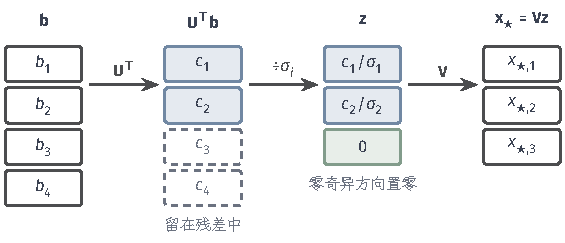
\includegraphics[width=95.652mm]{figures/01-basic-mathematics/03-vectors-matrices-and-multivariate-functions/tikz/c5-svd-solve-coordinates/figure.pdf}
  \caption{SVD求解的坐标变换，示意$m=4$、$d=3$、$r=2$。右端先变到左奇异坐标，蓝色的前$r$个坐标可以拟合，虚线框中的其余坐标无论怎样选$\bm x$都留在残差中；可拟合坐标除以对应奇异值，零奇异方向的坐标取零；最后由右奇异向量还原为原变量。}
  \label{fig:ls-svd-solve-coordinates}
\end{figure}

\paragraph{目标在奇异坐标下分离}
把未知量和右端分别换到右、左奇异坐标，令
\begin{equation}
 \bm z=\bm V^\top\bm x,\qquad \bm c=\bm U^\top\bm b .
 \label{eq:ls-svd-coordinates}
\end{equation}
由$\bm A\bm x=\bm U\bm\Sigma\bm z$，残差变为
\[
 \bm b-\bm A\bm x=\bm U(\bm c-\bm\Sigma\bm z),
\]
其中
\[
 \bm c-\bm\Sigma\bm z=(c_1-\sigma_1z_1,\ \ldots,\ c_r-\sigma_rz_r,\ c_{r+1},\ \ldots,\ c_m)^\top .
\]
由$\bm U$保持长度，
\begin{equation}
 \begin{aligned}
 \lVert\bm b-\bm A\bm x\rVert_2^2&=\lVert\bm c-\bm\Sigma\bm z\rVert_2^2\\
 &=\sum_{i=1}^r(c_i-\sigma_iz_i)^2+\sum_{i=r+1}^mc_i^2 .
 \end{aligned}
 \label{eq:ls-svd-coordinate-split}
\end{equation}
输入坐标$z_{r+1},\ldots,z_d$根本不出现在目标中。

\paragraph{逐个坐标求解}
式~\eqref{eq:ls-svd-coordinate-split}的各平方项互不耦合，可以分别取最小。对每个正奇异值令$c_i-\sigma_iz_i=0$，得
\begin{equation}
 z_i=\frac{c_i}{\sigma_i},\qquad i=1,\ldots,r ;
 \label{eq:ls-svd-coordinate-solution}
\end{equation}
输出端$i>r$的分量$c_i$无论怎样选$\bm x$都留在残差中。所以最小二乘解的全部自由度恰好是输入零空间方向上的坐标$z_{r+1},\ldots,z_d$。

\paragraph{取最小范数}
再由
\[
 \lVert\bm x\rVert_2=\lVert\bm V\bm z\rVert_2=\lVert\bm z\rVert_2 ,
\]
令全部自由坐标为零就使范数最小，得到
\begin{equation}
 \bm x_\star=\sum_{i=1}^r\frac{\bm u_i^\top\bm b}{\sigma_i}\bm v_i .
 \label{eq:ls-svd-solution}
\end{equation}
这给出了执行顺序：先把右端投影到输出奇异方向，再对正奇异值取逆，最后由输入奇异方向重建。它恰是伪逆作用于右端的结果，证明见本节的算法分析。

\subsection{算法实现}

输入是$\bm A\in\mathbb R^{m\times d}$与$\bm b\in\mathbb R^m$，不要求满秩，输出是最小范数最小二乘解$\bm x_\star$，没有额外需要选定的规则。这里按精确的秩$r$描述求解；有限精度下怎样判定数值秩，以及是否截断小奇异值，属于第~\ref{chap:solution-error-regularization}章的内容（第~\ref{sec:ls-pseudoinverse-rank-change}节与第~\ref{sec:ls-tsvd-solve}节）。

算法由两个模块组成：计算SVD取得因子，由奇异坐标求解。

下面用以下数据逐步演示：
\[
 \bm A=\begin{bmatrix}1&1\\1&1\end{bmatrix},\qquad
 \bm b=\begin{bmatrix}1\\3\end{bmatrix}.
\]
两个方程要求$x_1+x_2$同时等于$1$和$3$，方程不相容；$\bm A$的秩为$1$，最小二乘解也不唯一。

\subsubsection{计算SVD}
输入$\bm A$，输出$\bm U_r=[\bm u_1,\ldots,\bm u_r]$、$\bm\Sigma_r=\operatorname{diag}(\sigma_1,\ldots,\sigma_r)$与$\bm V_r=[\bm v_1,\ldots,\bm v_r]$。调用数值SVD过程，按第~\ref{chap:singular-value-decomposition}章的形式取得$\bm A=\bm U_r\bm\Sigma_r\bm V_r^\top$，其中$r=\operatorname{rank}\bm A$，$\bm U_r$与$\bm V_r$的列标准正交，各$\sigma_i>0$。若$\bm A=\bm0$，则直接取$\bm x_\star=\bm0$并结束。

例中$\bm A$的秩为$r=1$，唯一的正奇异值为$\sigma_1=2$，
\[
 \bm A=2\,\bm u_1\bm v_1^\top,\qquad
 \bm u_1=\bm v_1=\frac1{\sqrt2}\begin{bmatrix}1\\1\end{bmatrix};
\]
补齐后的另一对奇异方向
\[
 \bm u_2=\bm v_2=\frac1{\sqrt2}\begin{bmatrix}1\\-1\end{bmatrix}
\]
对应零奇异值，不进入薄分解。

\subsubsection{由奇异坐标求解}
输入$\bm U_r$、$\bm\Sigma_r$、$\bm V_r$与$\bm b$，输出$\bm x_\star$。
\begin{enumerate}
 \item \textbf{投影右端。}对$i=1,\ldots,r$计算
 \[
  c_i=\bm u_i^\top\bm b ,
 \]
 把右端投影到能够拟合的输出方向上；$\bm b$在其余方向上的部分，无论怎样选$\bm x$都会留在残差中。

 例中可拟合分量与被舍弃方向上的分量分别为
 \[
  c_1=\bm u_1^\top\bm b=2\sqrt2,\qquad \bm u_2^\top\bm b=-\sqrt2 .
 \]

 \item \textbf{按奇异值缩放。}根据主要思想中的逐个坐标求解，对$i=1,\ldots,r$计算
 \[
  z_i=\frac{c_i}{\sigma_i} .
 \]
 除法只对正奇异值进行，零奇异值对应的坐标取零。

 例中
 \[
  z_1=\frac{2\sqrt2}2=\sqrt2 .
 \]

 \item \textbf{还原原变量。}根据式~\eqref{eq:ls-svd-solution}，计算
 \[
  \bm x_\star=\bm V_r\bm z=\sum_{i\leq r}z_i\bm v_i .
 \]
 
 例中
 \[
  \bm x_\star=\sqrt2\cdot\frac1{\sqrt2}\begin{bmatrix}1\\1\end{bmatrix}=\begin{bmatrix}1\\1\end{bmatrix}.
 \]

 \item \textbf{输出并核验。}输出$\bm x_\star$，并用原始数据检查$\bm A^\top(\bm b-\bm A\bm x_\star)=\bm0$与$\bm x_\star\perp\ker\bm A$。

 例中拟合值与残差为
 \[
  \bm A\bm x_\star=\begin{bmatrix}2\\2\end{bmatrix},\qquad
  \bm b-\bm A\bm x_\star=\begin{bmatrix}-1\\1\end{bmatrix}.
 \]
 拟合值取两个观测的平均，残差与列空间方向$(1,1)^\top$正交，长度$\sqrt2$等于被舍弃分量的绝对值$\lvert\bm u_2^\top\bm b\rvert$。

 另一方面，$\bm x_\star$与核方向$(1,-1)^\top$正交：全部最小二乘解为$(1+t,1-t)^\top$，范数平方为
 \[
  (1+t)^2+(1-t)^2=2+2t^2 ,
 \]
 $t=0$时最小。
\end{enumerate}
整个过程只用到因子对向量的作用，无需形成完整的伪逆。

\subsection{算法分析}

\paragraph{正确性}
上述过程算出的正是伪逆作用于右端的结果。

\begin{theorem}[SVD求解给出\texorpdfstring{$\bm A^\dagger\bm b$}{A+b}]
\label{thm:ls-svd-solve}
对任意$\bm A\in\mathbb R^{m\times d}$与$\bm b\in\mathbb R^m$，上述过程的输出$\bm x_\star=\bm A^\dagger\bm b$，它是唯一的最小范数最小二乘解。
\end{theorem}
\begin{proof}
由式~\eqref{eq:matrix-analysis-pseudoinverse}，
\[
 \bm A^\dagger\bm b=\sum_{i\leq r}\frac{\bm v_i\bm u_i^\top\bm b}{\sigma_i},
\]
与输出相同；$\bm A=\bm0$时两者都是$\bm0$。最优性由定理~\ref{thm:matrix-analysis-pseudoinverse-minimum-norm}给出。也可以直接验证：残差$\bm b-\bm A\bm x_\star=\bm b-\bm U_r\bm U_r^\top\bm b$与列空间正交，所以$\bm x_\star$满足正规方程；$\bm x_\star\in\operatorname{range}(\bm V_r)=(\ker\bm A)^\perp$，由定理~\ref{thm:ls-minimum-norm-representative}，它在全部最小二乘解中范数最小。
\end{proof}

\paragraph{数值敏感度}
敏感性来自除以小奇异值。固定$\bm A$且$r>0$时，右端扰动$\delta\bm b$使解改变
\begin{equation}
 \begin{gathered}
 \delta\bm x_\star=\sum_{i=1}^r\frac{\bm u_i^\top\delta\bm b}{\sigma_i}\bm v_i,\\
 \lVert\delta\bm x_\star\rVert_2\leq\frac{\lVert\delta\bm b\rVert_2}{\sigma_r},
 \end{gathered}
 \label{eq:ls-svd-perturbation-bound}
\end{equation}
即放大倍数至多为$1/\sigma_r$。

稳定地算出SVD并不能消除问题本身的病态：分解残差很小，恢复出的系数仍可能被观测误差严重放大。若为了压低放大而截去真实的正奇异值，求的就已不是$\bm A^\dagger\bm b$，这属于第~\ref{chap:solution-error-regularization}章的截断SVD与正则化。

\subsection{加权最小二乘}
\label{sec:ls-weighted-svd-solve}

\subsubsection{主要思想}
第~\ref{sec:ls-weighted-ls}节的加权最小二乘以对称正定的权矩阵$\bm M\in\mathbb R^{m\times m}$规定目标函数$(\bm A\bm x-\bm b)^\top\bm M(\bm A\bm x-\bm b)$。核心思想是把权矩阵写成$\bm M=\bm R^\top\bm R$，代入目标函数得
\begin{equation}
 \begin{aligned}
 (\bm A\bm x-\bm b)^\top\bm M(\bm A\bm x-\bm b)
 &=\bigl(\bm R(\bm A\bm x-\bm b)\bigr)^\top\bigl(\bm R(\bm A\bm x-\bm b)\bigr)\\
 &=\lVert\bm R\bm A\bm x-\bm R\bm b\rVert_2^2 .
 \end{aligned}
 \label{eq:ls-weighted-whitening}
\end{equation}
所以用同一个$\bm R$变换$\bm A$和$\bm b$，记
\begin{equation}
 \widetilde{\bm A}=\bm R\bm A,\qquad \widetilde{\bm b}=\bm R\bm b ,
 \label{eq:ls-weighted-transformed-data}
\end{equation}
问题就成为普通最小二乘，对它调用SVD求解得到$\widetilde{\bm A}^\dagger\widetilde{\bm b}$。这一步称为白化。

$\bm R$的取法由$\bm M=\bm R^\top\bm R$决定。若Cholesky分解写作$\bm M=\bm L\bm L^\top$，必须取
\begin{equation}
 \bm R=\bm L^\top ,
 \label{eq:ls-weighted-cholesky-factor}
\end{equation}
才有$\bm R^\top\bm R=\bm L\bm L^\top$；取$\bm R=\bm L$则得到$\bm L^\top\bm L$，一般不等于$\bm M$。

对角权$\bm M=\operatorname{diag}(w_1,\ldots,w_m)$直接取
\begin{equation}
 \bm R=\operatorname{diag}(\sqrt{w_1},\ldots,\sqrt{w_m}) .
 \label{eq:ls-weighted-diagonal-factor}
\end{equation}

若权以$\bm M=\bm\Gamma^{-1}$的形式给出，$\bm\Gamma$为对称正定矩阵（例如观测误差的协方差），就分解$\bm\Gamma=\bm L\bm L^\top$，这时
\begin{equation}
 \bm M=\bm L^{-\top}\bm L^{-1},\qquad \bm R=\bm L^{-1},
 \label{eq:ls-weighted-covariance-factor}
\end{equation}
$\widetilde{\bm A}$与$\widetilde{\bm b}$由
\begin{equation}
 \bm L\widetilde{\bm A}=\bm A,\qquad \bm L\widetilde{\bm b}=\bm b
 \label{eq:ls-weighted-covariance-solve}
\end{equation}
按式~\eqref{eq:ls-forward-substitution}前代求出，不显式求逆。

变换只作用于观测端，未知量$\bm x$本身没有改变，所以白化后的解无须再变换回去；它为什么正是加权最小二乘解中欧氏范数最小的代表，见本小节的算法分析。权矩阵度量的是残差，不是系数，所以不能再把它当成系数范数的权重。

\subsubsection{算法实现}
输入是$\bm A$、$\bm b$与权矩阵$\bm M$，输出是加权最小二乘解中欧氏范数最小的代表$\bm x_\star$，没有额外需要选定的规则。

下面用以下数据逐步演示：
\[
 \bm A=\begin{bmatrix}1&1\\1&1\end{bmatrix},\qquad
 \bm b=\begin{bmatrix}0\\2\end{bmatrix},
\]
权矩阵为
\[
 \bm M=\begin{bmatrix}1&0\\0&3\end{bmatrix}.
\]
系数矩阵与第~\ref{sec:ls-svd-solve}节算法实现的例子相同，秩为$1$，加权解不唯一，两个观测的权重之比为$1:3$。
\begin{enumerate}
 \item \textbf{构造权因子。}按主要思想中的三种形式之一取得$\bm R$：一般情形作Cholesky分解$\bm M=\bm L\bm L^\top$并取$\bm R=\bm L^\top$，对角权取各权重的平方根，协方差形式分解$\bm\Gamma$。

 例中权为对角的，
 \[
  \bm R=\operatorname{diag}(1,\sqrt3) .
 \]

 \item \textbf{白化数据。}根据式~\eqref{eq:ls-weighted-whitening}，计算$\widetilde{\bm A}=\bm R\bm A$与$\widetilde{\bm b}=\bm R\bm b$；协方差形式改用前代。

 例中
 \[
  \widetilde{\bm A}=\begin{bmatrix}1&1\\\sqrt3&\sqrt3\end{bmatrix},\qquad
  \widetilde{\bm b}=\begin{bmatrix}0\\2\sqrt3\end{bmatrix}.
 \]

 \item \textbf{求解白化后的问题。}对$(\widetilde{\bm A},\widetilde{\bm b})$调用第~\ref{sec:ls-svd-solve}节的SVD求解，得到$\bm x_\star$并输出；$\widetilde{\bm A}$满列秩时也可以调用第~\ref{sec:ls-qr-method}节的QR求解。
 
 例中
 \[
  \widetilde{\bm A}=\begin{bmatrix}1\\\sqrt3\end{bmatrix}\begin{bmatrix}1&1\end{bmatrix},
 \]
 秩为$1$，唯一的正奇异值为
 \[
  \tilde\sigma_1=\lVert(1,\sqrt3)\rVert_2\,\lVert(1,1)\rVert_2=2\sqrt2,
 \]
 左、右奇异向量为
 \[
  \tilde{\bm u}_1=\frac12\begin{bmatrix}1\\\sqrt3\end{bmatrix},\qquad
  \tilde{\bm v}_1=\frac1{\sqrt2}\begin{bmatrix}1\\1\end{bmatrix}.
 \]
 投影与缩放得
 \[
  \tilde{\bm u}_1^\top\widetilde{\bm b}=3,\qquad
  z_1=\frac{3}{2\sqrt2},
 \]
 还原得
 \[
  \bm x_\star=\frac{3}{2\sqrt2}\cdot\frac1{\sqrt2}\begin{bmatrix}1\\1\end{bmatrix}=\begin{bmatrix}3/4\\3/4\end{bmatrix}.
 \]

 \item \textbf{核验。}用原始数据检查加权正规残差$\bm A^\top\bm M(\bm b-\bm A\bm x_\star)=\bm0$，需要最小范数时再检查$\bm x_\star\perp\ker\bm A$。

 例中拟合值为
 \[
  \bm A\bm x_\star=\begin{bmatrix}3/2\\3/2\end{bmatrix},
 \]
 两个观测的拟合值相同，取的是$0$与$2$按权重$1:3$的加权平均，而不是普通平均$1$。原残差及其加权为
 \[
  \bm r=\begin{bmatrix}-3/2\\1/2\end{bmatrix},\qquad
  \bm M\bm r=\begin{bmatrix}-3/2\\3/2\end{bmatrix},
 \]
 所以
 \[
  \bm A^\top\bm M\bm r=\bm0,\qquad
  \bm r^\top\bm M\bm r=\tfrac94+3\cdot\tfrac14=3 ,
 \]
 后者是加权残差平方。系数差的方向$(1,-1)^\top$张成$\ker\bm A$，$\bm x_\star$在这个方向上的分量为零。
\end{enumerate}

\subsubsection{算法分析}
由式~\eqref{eq:ls-weighted-whitening}，变换前后的目标函数逐点相等；未知量及其欧氏范数也没有变，所以两个问题的最优解集与最小范数代表都相同（定理~\ref{thm:ls-weighted-least-squares}）。又$\bm R$可逆，$\ker\widetilde{\bm A}=\ker\bm A$，所以$\bm x_\star\perp\ker\bm A$。

数值敏感度取决于$\widetilde{\bm A}=\bm R\bm A$而不是$\bm A$：权重可能改善条件，也可能使它变差，应在变换后的系统上判断。

\subsection{齐次最小二乘}
\label{sec:ls-homogeneous-svd-solve}

\subsubsection{主要思想}
第~\ref{sec:linear-algebra-homogeneous-estimation}节的齐次最小二乘在$\lVert\bm x\rVert_2=1$的约束下最小化$\lVert\bm A\bm x\rVert_2$。它是$\bm b=\bm0$的情形，单位长度约束属于求解目标，用来排除无意义的零解。核心思想是选择被$\bm A$伸缩得最小的方向。

用完整的右奇异基$\bm V=[\bm v_1,\ldots,\bm v_d]$写$\bm x=\bm V\bm z$。记$\hat\sigma_i=\lVert\bm A\bm v_i\rVert_2$为第$i$个方向的伸缩量：$i\leq\min(m,d)$时它是第$i$个奇异值（可以为零），$m<d$时多出的$d-m$个方向属于零空间，伸缩量为零。

由SVD，$\bm A\bm v_i=\hat\sigma_i\bm u_i$（伸缩量为零时为$\bm0$），各$\bm A\bm v_i$两两正交，于是约束与目标分别化为
\begin{equation}
 \lVert\bm x\rVert_2^2=\sum_{i=1}^dz_i^2=1,\qquad
 \lVert\bm A\bm x\rVert_2^2=\sum_{i=1}^d\hat\sigma_i^2z_i^2 .
 \label{eq:ls-homogeneous-coordinates}
\end{equation}
第二式是平方伸缩量$\hat\sigma_i^2$以$z_i^2$为权的加权平均，权的和为$1$，所以它不小于其中最小的一个$\hat\sigma_d^2$；把全部权放在最后一个坐标上就达到这个最小值，即
\begin{equation}
 \bm z=\pm\bm e_d,\qquad \hat{\bm x}=\bm V\bm z=\pm\bm v_d .
 \label{eq:ls-homogeneous-solution}
\end{equation}
最小值何时还在别的方向上达到，见本小节的算法分析。

\subsubsection{算法实现}
输入是$\bm A\in\mathbb R^{m\times d}$，输出是使$\lVert\bm A\bm x\rVert_2$最小的单位向量$\hat{\bm x}$，没有额外需要选定的规则。

下面用以下矩阵逐步演示：
\[
 \bm A=\begin{bmatrix}3&0\\0&1\\0&0\end{bmatrix}.
\]

\begin{enumerate}
 \item \textbf{计算完整右奇异基。}调用数值SVD过程，取得第~\ref{chap:singular-value-decomposition}章中的完整右因子$\bm V$，各列按伸缩量从大到小排列，并检查输入维数与秩。
 
 $m<d$时奇异值只有$m$个，完整右基中多出的方向属于零空间，也要保留；薄SVD可能没有列出全部右零空间，必须补齐相应的基，不能机械地取薄SVD的最后一列。
 
 这些方向直接从$\bm A$的SVD取得，不通过显式形成$\bm A^\top\bm A$再求特征向量。
 
 例中$\bm A$的两列已经正交，
 \[
  \sigma_1=3,\qquad \sigma_2=1,\qquad \bm V=\bm I,\quad\text{即}\quad \bm v_1=\bm e_1,\ \bm v_2=\bm e_2 ;
 \]
 $m>d$，无须补齐。

 \item \textbf{取最后一列。}令$\hat{\bm x}=\bm v_d$并输出：存在零空间时它是零空间中的单位向量，否则是最小正奇异值的右奇异向量。它已经是单位向量，无须再归一化；$\hat{\bm x}$与$-\hat{\bm x}$表示同一组参数比例。

 例中
 \[
  \hat{\bm x}=\bm e_2=\begin{bmatrix}0\\1\end{bmatrix},\qquad
  \lVert\bm A\hat{\bm x}\rVert_2=1 .
 \]

 \item \textbf{核验。}检查$\lVert\hat{\bm x}\rVert_2=1$，以及$\lVert\bm A\hat{\bm x}\rVert_2$等于最小伸缩量。

 例中在约束$x_1^2+x_2^2=1$下，目标为
 \[
  \lVert\bm A\bm x\rVert_2^2=9x_1^2+x_2^2=1+8x_1^2 ,
 \]
 在$x_1=0$时最小，最小残差范数为$1$，与$\hat{\bm x}=(0,\pm1)^\top$一致。零向量虽然给出零残差，却不满足单位长度约束。
\end{enumerate}

\subsubsection{算法分析}
正确性直接来自定理~\ref{thm:ls-homogeneous-minimizers}：$\lVert\bm A\bm x\rVert_2^2=\bm x^\top\bm A^\top\bm A\bm x$在单位球面上的最小值是$\bm A^\top\bm A$的最小特征值，由对应的特征向量达到，而$\bm v_d$正是这样的向量。

式~\eqref{eq:ls-homogeneous-coordinates}的加权平均论证给出同一结论，并刻画了全部最优解：加权平均等于最小值，当且仅当$\bm z$只落在取得最小伸缩量的那些坐标上。

所以最小伸缩量是单重的时，实数域中的最优方向只有$\pm\bm v_d$两个；重数大于一或零空间多于一维时，最优解是相应子空间中的全部单位向量，$\bm v_d$只是其中一个选择，应报告整个最优子空间，而不是声称有唯一的向量。

最优方向的敏感度由最小特征值与其余谱之间的间隙控制，可用第~\ref{sec:ls-subspace-sensitivity}节的子空间扰动界估计。单位长度与最优性的检验按第~\ref{sec:ls-least-squares-verification}节进行。

\section{方法选择与结果检验}
\label{sec:ls-direct-method-comparison}

前面各节分别给出了求最小二乘解与最小范数解的直接法。面对具体问题时，要先回到第~\ref{chap:linear-solution-selection}章确定的求解目标，再看矩阵的形状与秩，最后用原始数据核验算出的结果。本节按这一顺序归纳，并在同一组数据上比较几条路线。

\paragraph{按目标选择}
求最小二乘解时，满列秩用QR，条件数适中、需要按行累计数据时也可用正规方程法；满行秩欠定方程的最小范数解用转置QR；秩亏或秩未知的一般情形用SVD。加权目标先白化再按普通情形求解，齐次目标取最小伸缩方向。方阵且相容的精确解问题则回到第~\ref{chap:direct-linear-solvers}章，按矩阵结构选择LU、Cholesky或分块LDL。

\paragraph{同一组数据上的比较}
沿用示例~\ref{ex:ls-line-least-squares}的直线拟合$\bm A=\left[\begin{smallmatrix}1&0\\1&1\\1&2\end{smallmatrix}\right]$、$\bm b=(1,2,2)^\top$。正规方程法（示例~\ref{ex:ls-normal-equations-line-fit}）形成$\bm G=\left[\begin{smallmatrix}3&3\\3&5\end{smallmatrix}\right]$，得到Cholesky因子$\bm L$与前代结果$\bm y=(5/\sqrt3,1/\sqrt2)^\top$；Givens路线（示例~\ref{ex:ls-givens-line-fit}）得到$\bm R=\bm L^\top$与$\bm c_1=\bm y$，Householder路线（示例~\ref{ex:ls-householder-line-fit}）得到的$\bm R$与$\bm c_1$只差各行的符号。三条路线最后回代的是同一个三角方程，给出同一个$\hat{\bm x}=(7/6,1/2)^\top$；区别在得到这个方程的方式，正规方程法要先形成$\bm A^\top\bm A$，正交方法不需要。

复制常数列后得到$\widetilde{\bm A}=\left[\begin{smallmatrix}1&0&1\\1&1&1\\1&2&1\end{smallmatrix}\right]$，列空间和最优残差都不变，但秩降为$2$，正规方程与QR回代都会遇到零主元。SVD求解略去$\sigma_3=0$对应的方向$(1,0,-1)^\top/\sqrt2$，得到最小范数解$\bm x_\star=(7/12,1/2,7/12)^\top$：最小二乘只约束$x_1+x_3=7/6$与$x_2=1/2$，最小范数再把$7/6$平分给两个相同的列。前一组比较的差别在计算方式，这里的差别则在选解目标。

\paragraph{用原始数据核验}
算出$\bm x$后，要代回原问题检查它是否符合目标，而不只检查中间的小系统。普通最小二乘解检查$\bm A^\top(\bm b-\bm A\bm x)=\bm0$，要求最小范数时再检查$\bm x\perp\ker\bm A$。在上例中，残差$(-\tfrac16,\tfrac13,-\tfrac16)^\top$不为零，但它与$\bm A$的两列都正交；$\widetilde{\bm A}\bm x_\star=\bm A\hat{\bm x}$，且$\bm x_\star$与核方向$(1,0,-1)^\top$正交。加权问题使用第~\ref{sec:ls-least-squares-verification}节的加权正交条件$\bm A^\top\bm M(\bm b-\bm A\bm x)=\bm0$，齐次问题检查单位长度以及是否为最小伸缩方向。最小二乘的残差本来就可以非零；这些量用于核对计算过程，各求解算法仍只返回$\bm x$。

计算中还可以用分解残差（如$\lVert\bm A-\bm Q_1\bm R\rVert$）和正交性（如$\lVert\bm Q_1^\top\bm Q_1-\bm I\rVert$）分别核对中间变换，但这些检查只是旁证，不属于算法本身，也不能代替对原问题的检验。

\paragraph{残差小不等于误差小}
即使上述检验都通过，也不保证$\bm x$的误差小：矩阵接近奇异时，很小的残差可能对应很大的解误差。本章只给出了算法层面的结论：正规方程使条件数平方，正交变换保持长度，SVD把小奇异值的放大暴露为$1/\sigma_r$。第~\ref{chap:solution-error-regularization}章用条件数与前向、后向误差系统地解释这些现象（第~\ref{sec:ls-numerical-sensitivity}节），并在直接法与迭代法之间作整体比较（第~\ref{sec:ls-method-selection}节）。

\FloatBarrier
\section{本章小结}
\label{sec:direct-least-squares-summary}

本章回答了章首的问题：求解目标是最小二乘解或最小范数解时，怎样不求逆、不显式形成不必要的矩阵，在有限步内把选定的解算出来。三条路线的区别在于怎样处理$\bm A$。

正规方程法利用残差正交化为对称正定方程，再用上一章的Cholesky分解与三角代入求解；它可以按行累计数据，但使条件数平方，只适合条件较好的满列秩问题。QR求解用正交变换保持残差长度，把目标分成可消去的部分和不可拟合的部分，满列秩时回代$\bm R\hat{\bm x}=\bm c_1$，满行秩时对$\bm A^\top$分解得到最小范数解。

三种QR实现的差别在于怎样计算正交因子。修正Gram--Schmidt直接算出正交基，有限精度下可能失去正交性；Householder反射一次消去整列，选取同号符号避免相消，是稠密问题的标准做法；Givens旋转一次消去一个元素，适合稀疏结构和逐行更新。秩亏或秩未知时，SVD求解在奇异坐标下把目标分离成独立的标量问题，对任意形状和秩给出$\bm A^\dagger\bm b$；加权问题经白化化为普通情形，齐次问题取完整右奇异基中伸缩量最小的方向。

无论用哪种方法，结果都要回到原始数据上按目标检验：最小二乘解看残差是否与列空间正交，最小范数解还要看是否与零空间正交。这些检验说明算出的$\bm x$符合目标，却不说明它离真解有多近。条件数平方和小奇异值的放大在本章只作了算法层面的说明，结果的可信程度、数值秩的判定以及正则化留给第~\ref{chap:solution-error-regularization}章。矩阵太大而无法分解，或只能通过矩阵与向量的乘积访问矩阵时，就需要从第~\ref{chap:stationary-iterations}章开始的迭代法。


% 定常迭代法：矩阵分裂、Richardson、Jacobi、Gauss--Seidel、SOR、SSOR与停止准则
\chapter{定常迭代法}
\label{sec:ls-stationary-iterations}
\label{chap:stationary-iterations}

设$\bm A\in\mathbb R^{d\times d}$可逆，要解$\bm A\bm x=\bm b$。第~\ref{chap:direct-linear-solvers}章的直接法先分解$\bm A$再回代，要存储并计算分解因子。矩阵很大而稀疏时，消元会在原来的零元位置产生大量非零元（填充），因子的存储和运算都可能难以承受。

本章换一条路线。选一个容易求解、又与$\bm A$相近的矩阵$\bm M$，每轮根据当前残差，解一个以$\bm M$为系数的方程得到修正量，再把修正量加到近似解上。每轮只需一次矩阵乘向量和一次简单求解（对角缩放或三角求解），不需要存储分解因子。这样做立即带来几个问题：这种更新从任意初值出发何时收敛到真解，收敛有多快，每轮要花多少计算，以及什么时候可以停下来。

回答收敛问题的工具来自第~\ref{chap:linear-recurrence-stability}章。那里证明了：仿射迭代$\bm x\mapsto\bm T\bm x+\bm c$从任意初值出发都收敛到同一个极限，当且仅当$\bm T$的谱半径小于一；渐近的收敛速度由谱半径决定，而非正规的$\bm T$在衰减之前还可能暂时放大误差。本章把每种方法都写成这种形式，收敛判断便归结为估计相应迭代矩阵的谱半径。三角求解采用第~\ref{sec:ls-lu}节的前代与回代。

第~\ref{sec:ls-matrix-splitting}节建立各方法共用的框架：由矩阵分裂得到不动点方程与修正形式，统一的执行流程，以及由谱半径给出的收敛判据。随后五节分别取不同的$\bm M$：Richardson迭代用标量矩阵，Jacobi迭代用$\bm A$的对角部分，Gauss--Seidel迭代用下三角部分，SOR在下三角修正中加入松弛参数，SSOR把前向与反向两次扫掠配成对称的一轮。此后每节先简述所取的$\bm M$与迭代形式，再分算法实现与算法分析两部分；算法实现逐步写出执行公式，并用同一个二维例子逐轮计算，便于对照各方法读取数据的方式。

SSOR的修正矩阵对称正定，这使它还能作为第~\ref{chap:krylov-methods}章共轭梯度法的预条件。最后一节讨论停止准则：达到残差要求与只是停止计算是两回事。

记号沿用本部分的约定：精确解记作$\bm x_\star$，第$k$轮近似记作$\bm x_k$，残差$\bm r_k=\bm b-\bm A\bm x_k$，修正量$\bm\delta_k$，误差$\bm e_k=\bm x_k-\bm x_\star$；向量的第$i$个分量写作$(\bm x_k)_i$。

\section{定常迭代}
\label{sec:ls-matrix-splitting}

\subsection{算法思想}

定常迭代的思路可以概括为两步：先把难解的方程拆成“容易求解的部分”与“其余部分”，从而改写成不动点方程；再从任意初值出发，用同一个固定的映射反复更新。

\paragraph{矩阵分裂}
直接求解$\bm A\bm x=\bm b$相当于处理$\bm A^{-1}$，对一般的$d$阶矩阵要做约$d^3$量级的运算。

我们可以换一个思路：把$\bm A$拆成两部分，
\begin{equation}
 \bm A=\bm M-\bm N ,
 \label{eq:ls-stationary-splitting}
\end{equation}
其中$\bm M$可逆并且极易求解，例如对角矩阵或三角矩阵，$\bm N=\bm M-\bm A$是剩下的部分。这种拆法称为\term{矩阵分裂}（matrix splitting）。

代入原方程，得
\[
 (\bm M-\bm N)\bm x=\bm b,\qquad\text{即}\qquad \bm M\bm x=\bm N\bm x+\bm b .
\]
两边左乘$\bm M^{-1}$，方程化为
\begin{equation}
 \bm x=\bm T\bm x+\bm c
 \label{eq:ls-stationary-fixed-point}
\end{equation}
其中$
 \bm T=\bm M^{-1}\bm N=\bm I-\bm M^{-1}\bm A$，$\bm c=\bm M^{-1}\bm b$。
这是一个\term{不动点方程}（fixed-point equation）：$\bm x_\star$正是仿射映射$\bm x\mapsto\bm T\bm x+\bm c$的不动点。$\bm T$称为\term{迭代矩阵}（iteration matrix），$\bm c$是常向量。

\paragraph{迭代求解}
有了不动点方程，自然的做法是把右端算出的值作为下一个近似，得到递推
\begin{equation}
 \bm x_{k+1}=\bm T\bm x_k+\bm c .
 \label{eq:ls-stationary-iteration}
\end{equation}
若$\bm x_k$收敛，极限必然满足式~\eqref{eq:ls-stationary-fixed-point}，也就是原方程的解。

整个过程中$\bm T$和$\bm c$固定不变，每一轮都用同一套规则修正当前的解，所以这类方法称为\term{定常迭代}（stationary iteration）。第~\ref{chap:krylov-methods}章的Krylov子空间法则不同：每一轮的搜索方向和步长系数都要由当前残差重新计算，相当于每轮的更新规则都在变化。

\paragraph{修正的迭代求解}
式~\eqref{eq:ls-stationary-iteration}中的$\bm M^{-1}$只是理论表示，执行时不形成逆矩阵。把它乘回去，得
\[ 
  \bm M\bm x_{k+1}=\bm N\bm x_k+\bm b=\bm M\bm x_k+(\bm b-\bm A\bm x_k) .
\]
记残差$\bm r_k=\bm b-\bm A\bm x_k$，修正量$\bm\delta_k=\bm x_{k+1}-\bm x_k$，就得到等价的修正形式
\begin{equation}
 \bm M\bm\delta_k=\bm r_k,\qquad \bm x_{k+1}=\bm x_k+\bm\delta_k .
 \label{eq:ls-stationary-correction}
\end{equation}
每轮只需算一次残差，再解一个以$\bm M$为系数的方程。

这个形式也说明了$\bm M$的作用。式~\eqref{eq:ls-stationary-correction}用$\bm M$代替了$\bm A$，只解近似的修正方程。$\bm M$越接近$\bm A$，修正越准确，但求解也越接近原问题的难度；$\bm M$越简单，每轮越便宜，修正却越粗糙。所以$\bm M$同时决定单步成本与每轮消除误差的程度。“容易求解”只说明每轮算得下去，并不保证迭代收敛，收敛要另行判断。

\paragraph{执行过程} 按这一形式，整个算法的执行流程如下。

先算$\bm r_0=\bm b-\bm A\bm x_0$，取停止阈值$\tau=\mathrm{atol}+\mathrm{rtol}\lVert\bm b\rVert_2$。

每一轮依次做三件事：
\begin{enumerate}
 \item \textbf{停止检查。}若$\lVert\bm r_k\rVert_2\leq\tau$，以“达到容差”结束；若$k=K$，以“步数耗尽”结束；出现溢出或非数时以“数值异常”结束，残差长期几乎不降时可报告“停滞”。只有第一种表示达到了残差目标，第~\ref{sec:ls-stationary-stopping}节再解释。
 \item \textbf{求修正量。}按式~\eqref{eq:ls-stationary-correction}解$\bm M\bm\delta_k=\bm r_k$；这一步随$\bm M$的选取而不同，是后面各节的主要内容。
 \item \textbf{更新。}令$\bm x_{k+1}=\bm x_k+\bm\delta_k$，按原方程重算$\bm r_{k+1}=\bm b-\bm A\bm x_{k+1}$，再令$k\leftarrow k+1$回到停止检查。
\end{enumerate}

后面各方法都沿用这套流程，只替换求$\bm\delta_k$的一步。

后面各方法用同一个小例子对照。下面先取对角矩阵作$\bm M$，只为核对流程中每个量怎样得到。
\begin{example}[定常迭代的贯穿例]
\label{ex:ls-stationary-running-example}
取下面的系数矩阵与右端，初值为$\bm x_0=\bm 0$：
\[
\bm A=\begin{bmatrix}4&1\\1&3\end{bmatrix},\qquad
\bm b=\begin{bmatrix}1\\2\end{bmatrix}.
\]
精确解为$\bm x_\star=(1/11,7/11)^\top\approx(0.0909,0.6364)^\top$。

取$\bm M=\operatorname{diag}(4,3)$，解修正方程只需逐分量相除。第一轮从$\bm r_0=\bm b$出发，修正量与新的近似解为
\[
 \bm\delta_0=\begin{bmatrix}\tfrac14\\\tfrac23\end{bmatrix},\qquad
 \bm x_1=\begin{bmatrix}\tfrac14\\\tfrac23\end{bmatrix},
\]
按原方程算出的残差为
\[
 \bm r_1=\bm b-\bm A\bm x_1=\begin{bmatrix}-\tfrac23\\-\tfrac14\end{bmatrix}.
\]
第二轮同样先求修正量并更新：
\[
 \bm\delta_1=\begin{bmatrix}-\tfrac16\\-\tfrac1{12}\end{bmatrix},\qquad
 \bm x_2=\begin{bmatrix}\tfrac1{12}\\\tfrac7{12}\end{bmatrix},
\]
再算出残差
\[
 \bm r_2=\begin{bmatrix}\tfrac1{12}\\\tfrac16\end{bmatrix}.
\]
残差范数依次约为$2.24$、$0.71$、$0.19$，在下降但没有降到零。每轮的修正方程都精确地解出了，$\bm x_2$却仍不是解，因为修正方程用$\bm M$代替了$\bm A$；是否解完，只能由原方程的残差判断。
\end{example}

\paragraph{按元素构造分裂}
后面的方法要按元素构造$\bm M$，为此统一写
\begin{equation}
\bm A=\bm D+\bm L+\bm U ,
 \label{eq:ls-stationary-dlu-splitting}
\end{equation}
其中$\bm D$是$\bm A$的对角部分，$\bm L$与$\bm U$分别是严格下三角与严格上三角部分，元素保留$\bm A$中原来的符号。

\subsection{算法分析}

精确解满足$\bm x_\star=\bm T\bm x_\star+\bm c$，与式~\eqref{eq:ls-stationary-iteration}相减，误差$\bm e_k=\bm x_k-\bm x_\star$满足
\[
 \bm e_{k+1}=\bm T\bm e_k=(\bm I-\bm M^{-1}\bm A)\bm e_k .
\]
每轮误差乘同一个固定矩阵，这正是第~\ref{chap:linear-recurrence-stability}章研究过的矩阵幂问题，下面据此给出收敛判据。

\paragraph{收敛条件}
各方法是否收敛，取决于迭代矩阵$\bm T=\bm I-\bm M^{-1}\bm A$每轮把误差变成什么。下面的定理把收敛问题归结为$\bm T$的谱半径，后面各节只需分别估计各自的$\rho(\bm T)$。
\begin{theorem}[定常迭代的收敛判据]
\label{thm:ls-stationary-convergence}
设$\bm A$与$\bm M$可逆，$\bm x_\star$是$\bm A\bm x=\bm b$的解。按$\bm M\bm\delta_k=\bm r_k$，$\bm x_{k+1}=\bm x_k+\bm\delta_k$迭代时，误差满足
\begin{equation}
\bm e_{k+1}=\bm T\bm e_k,\qquad \bm e_k=\bm T^k\bm e_0 ,
 \label{eq:ls-stationary-error-recursion}
\end{equation}
且迭代对任意初值$\bm x_0$都收敛到$\bm x_\star$，当且仅当$\rho(\bm T)<1$。
\end{theorem}
\begin{proof}
由$\bm r_k=\bm b-\bm A\bm x_k=-\bm A\bm e_k$，更新式给出
\[
 \bm e_{k+1}=\bm e_k-\bm M^{-1}\bm A\bm e_k=\bm T\bm e_k ,
\]
归纳得$\bm e_k=\bm T^k\bm e_0$。

更新也可写成仿射映射$\bm x\mapsto\bm T\bm x+\bm M^{-1}\bm b$。因为$\bm I-\bm T=\bm M^{-1}\bm A$可逆，它只有一个固定点，满足$\bm M^{-1}\bm A\bm x=\bm M^{-1}\bm b$，就是$\bm x_\star$。

由第~\ref{sec:ls-convergence}章的定理~\ref{thm:ls-affine-common-limit}，从任意初值出发的轨迹都收敛到同一个向量当且仅当$\rho(\bm T)<1$，而这个共同极限只能是固定点$\bm x_\star$。
\end{proof}

算法可执行与算法收敛是两个条件：$a_{i,i}\neq0$只保证每轮能算下去，不保证$\rho(\bm T)<1$；反过来，$\rho(\bm T)<1$也不保证某种逐元素公式可以执行。

\paragraph{收敛速度与总成本}
渐近速度由$\bm T$的谱控制：由定理~\ref{thm:ls-gelfand-formula}，$\lVert\bm T^k\rVert^{1/k}\to\rho(\bm T)$，误差每缩小十倍约需$1/\log_{10}(1/\rho(\bm T))$轮。非正规的$\bm T$还可能在衰减前暂时放大误差（第~\ref{sec:ls-convergence-rate-transient}节），所以前几轮的表现不能代替渐近判断。

收缩率与单步成本是两件事。达到给定精度的总工作量约为所需轮数乘每轮成本；每轮成本包括一次求$\bm\delta_k$和一次计算残差的矩阵乘向量。$\bm M$越接近$\bm A$，谱半径通常越小，但求解$\bm M$越贵。比较不同分裂时要把两者合起来看，不能只比较谱半径或只比较单步成本。

\section{Richardson迭代}
\label{sec:ls-richardson}

最简单的选择是用标量矩阵代替$\bm A$：取非零步长$\alpha$，令修正矩阵$\bm M=\alpha^{-1}\bm I$。这相当于认为$\bm A$在各个方向上都大致把向量放大$1/\alpha$倍。迭代矩阵为$\bm T=\bm I-\alpha\bm A$，常向量为$\bm c=\alpha\bm b$。

$\bm M$是单位矩阵的倍数，修正方程$\alpha^{-1}\bm\delta_k=\bm r_k$两边乘以$\alpha$就解出了修正量：
\begin{equation}
 \bm\delta_k=\alpha\bm r_k ,\qquad\text{即}\qquad (\bm\delta_k)_i=\alpha(\bm r_k)_i .
 \label{eq:ls-richardson-correction}
\end{equation}
每个残差分量按同一比例转成对应分量的修正，不需要读取$\bm A$的任何元素。

把修正量加到当前近似上，一轮迭代就是
\begin{equation}
 \bm x_{k+1}=\bm x_k+\alpha(\bm b-\bm A\bm x_k)=(\bm I-\alpha\bm A)\bm x_k+\alpha\bm b .
 \label{eq:ls-richardson-update}
\end{equation}

\subsection{算法实现}

输入是$\bm A$与$\bm b$，输出是近似解$\bm x$。除第~\ref{sec:ls-matrix-splitting}节执行流程中的初值、容差与最大轮数外，还要预先选定步长$\alpha$。下面在例~\ref{ex:ls-stationary-running-example}上取$\alpha=1/4$，每一步之后给出前两轮的数值。
\begin{enumerate}
 \item \textbf{核对步长。}使用对称正定情形的收敛保证（定理~\ref{thm:ls-richardson-spd}）时，先按已知的谱界核对
 \begin{equation}
  0<\alpha<\frac{2}{\lambda_{\max}} ;
  \label{eq:ls-richardson-step-range}
 \end{equation}
 
 例中$\bm A$对称正定，最大特征值为$(7+\sqrt5)/2\approx4.618<5$，所以$2/\lambda_{\max}>2/5>1/4$，步长$\alpha=1/4$在收敛区间内。

 \item \textbf{求修正量。}通过停止检查后，按式~\eqref{eq:ls-richardson-correction}把残差的每个分量乘以同一个步长：
 \[
  (\bm\delta_k)_i=\alpha(\bm r_k)_i,\qquad i=1,\ldots,d .
 \]

 例中第一轮的残差为$\bm r_0=\bm b-\bm A\bm 0=(1,2)^\top$，于是
 \[
  \bm\delta_0=\frac14\begin{bmatrix}1\\2\end{bmatrix}=\begin{bmatrix}\tfrac14\\\tfrac12\end{bmatrix}.
 \]

 \item \textbf{更新并重算残差。}令$\bm x_{k+1}=\bm x_k+\bm\delta_k$，再用原矩阵算一次$\bm q_{k+1}=\bm A\bm x_{k+1}$，得到残差$\bm r_{k+1}=\bm b-\bm q_{k+1}$。按分量写出就是
 \begin{equation}
  (\bm r_{k+1})_i=b_i-\sum_{j=1}^d a_{i,j}(\bm x_{k+1})_j ,\qquad i=1,\ldots,d .
  \label{eq:ls-stationary-residual-update}
 \end{equation}
 重算的残差既用于下一轮的停止检查，也是下一轮修正的输入，所以每轮只需一次矩阵乘向量。

 例中$\bm x_1=\bm 0+\bm\delta_0=(1/4,1/2)^\top$，
 \[
  \begin{aligned}
  (\bm r_1)_1&=1-\bigl(4\cdot\tfrac14+1\cdot\tfrac12\bigr)=1-\tfrac32=-\tfrac12,\\
  (\bm r_1)_2&=2-\bigl(1\cdot\tfrac14+3\cdot\tfrac12\bigr)=2-\tfrac74=\tfrac14 .
  \end{aligned}
 \]

 \item \textbf{进入下一轮。}令$k\leftarrow k+1$，回到执行流程的停止检查；没有停止时重复第2、3步。

 例中$\lVert\bm r_1\rVert_2\approx0.56$，继续第二轮。修正量与新的近似解为
 \[
  \bm\delta_1=\frac14\bm r_1=\begin{bmatrix}-\tfrac18\\\tfrac1{16}\end{bmatrix},\qquad
  \bm x_2=\bm x_1+\bm\delta_1=\begin{bmatrix}\tfrac18\\\tfrac9{16}\end{bmatrix}.
 \]

\end{enumerate}

两轮后残差长度约为$0.198$。与精确解比较，误差为
\[
\bm e_2=\bm x_2-\bm x_\star=\begin{bmatrix}\tfrac3{88}\\-\tfrac{13}{176}\end{bmatrix},
\]
长度约$0.081$。由$\bm e_k=-\bm A^{-1}\bm r_k$，误差是残差经$\bm A^{-1}$变换后的结果，两者方向和大小都不同，是不同的数值对象。

\subsection{算法分析}

\paragraph{收敛条件与最优步长}
当$\bm A$实对称正定时，误差递推$\bm e_{k+1}=(\bm I-\alpha\bm A)\bm e_k$可以按特征方向分开看：把$\bm e_k$按$\bm A$的正交特征基展开，特征值$\lambda_i$对应的误差系数每轮乘$1-\alpha\lambda_i$。由定理~\ref{thm:ls-stationary-convergence}，收敛条件和最优步长都可以从这些倍率直接读出。
\begin{theorem}[对称正定矩阵的Richardson迭代]
\label{thm:ls-richardson-spd}
设$\bm A$实对称正定，特征值落在$[\lambda_{\min},\lambda_{\max}]$中且两端取到。Richardson迭代对所有初值收敛当且仅当$0<\alpha<2/\lambda_{\max}$；最优固定步长为$\alpha_\star=2/(\lambda_{\min}+\lambda_{\max})$，对应的收缩因子为
\begin{equation}
\rho(\bm T)=\frac{\kappa_2(\bm A)-1}{\kappa_2(\bm A)+1}.
 \label{eq:ls-richardson-optimal-rate}
\end{equation}
\end{theorem}
\begin{proof}
由上面的特征展开，
\[
 \rho(\bm T)=\max_i|1-\alpha\lambda_i| ,
\]
它小于一当且仅当每个$\alpha\lambda_i\in(0,2)$，即$0<\alpha<2/\lambda_{\max}$。

$|1-\alpha\lambda|$作为$\lambda$的函数在区间端点取最大，所以
\[
\rho(\bm T)=q(\alpha)=\max\{|1-\alpha\lambda_{\min}|,\ |1-\alpha\lambda_{\max}|\}.
\]
$\alpha$从零增大时，$|1-\alpha\lambda_{\min}|$先变小，$|1-\alpha\lambda_{\max}|$在$\alpha>1/\lambda_{\max}$后变大；两者大小相等、符号相反时最大值最小，即
\[
 1-\alpha\lambda_{\min}=\alpha\lambda_{\max}-1 ,
\]
解得$\alpha_\star$。代回得
\[
 q(\alpha_\star)=\frac{\lambda_{\max}-\lambda_{\min}}{\lambda_{\max}+\lambda_{\min}} ,
\]
再用$\kappa_2(\bm A)=\lambda_{\max}/\lambda_{\min}$即得式~\eqref{eq:ls-richardson-optimal-rate}。
\end{proof}
步长过大时，大特征值方向的倍率$1-\alpha\lambda_{\max}$小于$-1$，误差在该方向上正负交替地放大；所以残差没有消失并不意味着应当加大修正。

一般非对称矩阵仍可使用同一更新式，但特征值可能是复数，也没有正交特征基，上面的步长区间与最优步长不再直接适用；这时要回到定理~\ref{thm:ls-stationary-convergence}，检查$\rho(\bm I-\alpha\bm A)<1$。

\paragraph{收敛速度与代价}
谱范围越宽，$\kappa_2(\bm A)$越大，收缩因子越接近一，收敛越慢。实际中谱端点往往未知，步长按已知的谱界选取，例如用$\lVert\bm A\rVert$作$\lambda_{\max}$的上界。

贯穿例中$\lambda_{\min}\approx2.382$，$\lambda_{\max}\approx4.618$：$\alpha=1/4$时$\rho(\bm T)=1-\lambda_{\min}/4\approx0.40$；最优步长$\alpha_\star=2/7$给出$\rho(\bm T)=\sqrt5/7\approx0.32$。

每轮的主要代价是一次矩阵乘向量，约$2\operatorname{nnz}(\bm A)$次运算。停止时的残差与解误差之间的关系在第~\ref{sec:ls-stationary-stopping}节解释。

\section{Jacobi迭代}
\label{sec:ls-jacobi}

Richardson迭代对所有方程用同一个比例，没有利用各个方程自身的尺度。Jacobi迭代取$\bm A$的对角部分作修正矩阵，$\bm M=\bm D$：第$i$个方程只用来修正“自己的”未知量$x_i$，其余分量一律取上一轮的值。对角元相对非对角元越大，$\bm D$越接近$\bm A$，这个近似越好；例~\ref{ex:ls-stationary-running-example}所取的$\bm M=\operatorname{diag}(4,3)$正是这个分裂。

\paragraph{求修正量}
修正方程$\bm D\bm\delta_k=\bm r_k$的系数矩阵只有对角元，按元素写出是
\[
 \begin{bmatrix}a_{1,1}&&&\\&a_{2,2}&&\\&&\ddots&\\&&&a_{d,d}\end{bmatrix}
 \begin{bmatrix}(\bm\delta_k)_1\\(\bm\delta_k)_2\\\vdots\\(\bm\delta_k)_d\end{bmatrix}
 =\begin{bmatrix}(\bm r_k)_1\\(\bm r_k)_2\\\vdots\\(\bm r_k)_d\end{bmatrix},
\]
其中空白位置都是零。左边乘出来，第$i$行只剩对角元一项，所以按行的方程是
\[
 a_{i,i}(\bm\delta_k)_i=(\bm r_k)_i\qquad(i=1,\ldots,d).
\]
与前代不同，这里每个方程只含一个未知量，不需要用到其他方程的结果。两边除以$a_{i,i}$，得
\begin{equation}
 (\bm\delta_k)_i=\frac{(\bm r_k)_i}{a_{i,i}}\qquad(i=1,\ldots,d).
 \label{eq:ls-jacobi-correction}
\end{equation}
耦合的方程组就这样拆成了$d$个独立的标量计算，可以按任意次序或同时进行。

\paragraph{迭代公式}
把式~\eqref{eq:ls-jacobi-correction}加到当前近似上，得到第$i$个分量的新值
\begin{equation}
 (\bm x_{k+1})_i=(\bm x_k)_i+\frac{(\bm r_k)_i}{a_{i,i}}\qquad(i=1,\ldots,d),
 \label{eq:ls-jacobi-update}
\end{equation}
写成向量形式是
\[
  \bm x_{k+1}=\bm x_k+\bm D^{-1}\bm r_k .
\]

残差$\bm r_k$由上一轮的$\bm x_k$算出，所以各分量可以同时计算。

\subsection{算法实现}

输入是$\bm A$与$\bm b$，输出是近似解$\bm x$，执行流程的参数之外不需要其他参数。停止检查与残差重算沿用第~\ref{sec:ls-matrix-splitting}节的流程，求修正量的一步换成逐分量除以对角元。实现时维护新旧两个向量：旧向量$\bm x_k$在整轮中只读不写，新分量写进另一个向量。下面在例~\ref{ex:ls-stationary-running-example}上给出前两轮，并标明每个代入值的轮次。
\begin{enumerate}
 \item \textbf{检查对角元。}确认所有$a_{i,i}\neq0$，并保存倒数$1/a_{i,i}$。若某个对角元为零，当前的变量排列下方法不可执行；重排行列属于另一步，重排后要重新核对条件。

 例中$a_{1,1}=4$，$a_{2,2}=3$，都不为零。

 \item \textbf{逐分量计算新值。}根据式~\eqref{eq:ls-jacobi-update}，对$i=1,\ldots,d$计算$(\bm x_{k+1})_i$，其中的残差$\bm r_k$是由旧向量算出的。各分量只读旧向量和$\bm r_k$，彼此不依赖，可以按任意次序或并行计算。

 例中第一轮的残差为$\bm r_0=\bm b=(1,2)^\top$：
 \[
  \begin{aligned}
  (\bm x_1)_1&=(\bm x_0)_1+\frac{(\bm r_0)_1}{a_{1,1}}=0+\frac14=\frac14,\\
  (\bm x_1)_2&=(\bm x_0)_2+\frac{(\bm r_0)_2}{a_{2,2}}=0+\frac23=\frac23 .
  \end{aligned}
 \]

 \item \textbf{整体替换并重算残差。}全部$d$个分量算完之后，才用新向量替换旧向量，并按原方程重算
 \[
  (\bm r_{k+1})_i=b_i-\sum_{j=1}^d a_{i,j}(\bm x_{k+1})_j ,\qquad i=1,\ldots,d .
 \]
 若算出一个分量就覆盖旧值，再按新值重算后面的残差分量，后面的行就会读到本轮的新值，方法就不再是Jacobi迭代。单个分量变化很小，也不能代替这个全局残差检查。

 例中$\bm x_1=(1/4,2/3)^\top$，
 \[
  \begin{aligned}
  (\bm r_1)_1&=1-\bigl(4\cdot\tfrac14+1\cdot\tfrac23\bigr)=-\tfrac23,\\
  (\bm r_1)_2&=2-\bigl(1\cdot\tfrac14+3\cdot\tfrac23\bigr)=-\tfrac14 .
  \end{aligned}
 \]
 两个残差分量都变成负的，说明两个修正都过了头：每个分量都在假定另一个分量不变的前提下修正，而另一个分量同时也在变。

 \item \textbf{进入下一轮。}令$k\leftarrow k+1$，回到执行流程的停止检查；没有停止时重复第2、3步。

 例中$\lVert\bm r_1\rVert_2\approx0.71$，继续第二轮。用$\bm r_1=(-2/3,-1/4)^\top$修正$\bm x_1=(1/4,2/3)^\top$：
 \[
  \begin{aligned}
  (\bm x_2)_1&=(\bm x_1)_1+\frac{(\bm r_1)_1}{a_{1,1}}=\frac14-\frac{2/3}{4}=\frac1{12},\\
  (\bm x_2)_2&=(\bm x_1)_2+\frac{(\bm r_1)_2}{a_{2,2}}=\frac23-\frac{1/4}{3}=\frac7{12},
  \end{aligned}
 \]
 重算残差得
 \[
  \begin{aligned}
  (\bm r_2)_1&=1-\bigl(4\cdot\tfrac1{12}+1\cdot\tfrac7{12}\bigr)=\tfrac1{12},\\
  (\bm r_2)_2&=2-\bigl(1\cdot\tfrac1{12}+3\cdot\tfrac7{12}\bigr)=\tfrac16 .
  \end{aligned}
 \]
 结果与例~\ref{ex:ls-stationary-running-example}中按修正量计算的完全一致，残差长度由约$0.71$降到约$0.19$。
\end{enumerate}

\subsection{算法分析}

\paragraph{收敛条件}
Jacobi迭代矩阵$\bm T_{\mathrm J}=-\bm D^{-1}(\bm L+\bm U)$第$i$行的非对角元为$-a_{i,j}/a_{i,i}$，对角元为零。当每行的对角元压过同一行其余元素时，这个矩阵的行和范数小于一，由此得到常用的充分条件。

称$\bm A$\term{严格行对角占优}（strictly row diagonally dominant），如果每行都有$|a_{i,i}|>\sum_{j\neq i}|a_{i,j}|$。
\begin{theorem}[Jacobi迭代的收敛条件]
\label{thm:ls-jacobi-convergence}
若$\bm A$严格行对角占优，则
\begin{equation}
q=\lVert\bm T_{\mathrm J}\rVert_\infty=\max_i\frac{\sum_{j\neq i}|a_{i,j}|}{|a_{i,i}|}<1,
 \label{eq:ls-jacobi-contraction}
\end{equation}
Jacobi迭代对所有初值收敛，且$\lVert\bm e_k\rVert_\infty\leq q^k\lVert\bm e_0\rVert_\infty$。
\end{theorem}
\begin{proof}
$\infty$-范数诱导的矩阵范数等于最大行绝对值和，$\bm T_{\mathrm J}$第$i$行的绝对值和正是$\sum_{j\neq i}|a_{i,j}|/|a_{i,i}|$，对角占优使它小于一。由定理~\ref{thm:ls-stationary-convergence}，$\bm e_k=\bm T_{\mathrm J}^k\bm e_0$，再用范数的次乘性得$\lVert\bm e_k\rVert_\infty\leq q^k\lVert\bm e_0\rVert_\infty\to0$。
\end{proof}
贯穿例两行的比值分别为$1/4$与$1/3$，所以$q=1/3$。

对称正定本身并不够。$\bm A=\bm I+2\bm 1\bm 1^\top\in\mathbb R^{3\times3}$的特征值为$7,1,1$，是对称正定矩阵，而它的对角部分为$3\bm I$，于是
\[
 \bm T_{\mathrm J}=-\tfrac23(\bm 1\bm 1^\top-\bm I) .
\]
它沿$\bm 1$方向的特征值为$-\tfrac23(3-1)=-4/3$，在与$\bm 1$正交的方向上为$2/3$，所以$\rho(\bm T_{\mathrm J})=4/3$，迭代发散。

\paragraph{并行性}
各分量的更新互不依赖，可以并行；一轮工作量与$\operatorname{nnz}(\bm A)$同阶。单步便宜、易于并行，不等于误差衰减快：$\rho(\bm T_{\mathrm J})$接近一时需要很多轮。

\paragraph{数值敏感度}
式~\eqref{eq:ls-jacobi-correction}要除以对角元。很小的对角元会把残差分量放大成很大的修正，也放大其中的舍入误差。

\section{Gauss--Seidel迭代}
\label{sec:ls-gauss-seidel}

Jacobi迭代求第$i$个分量的修正时，只用本轮开始时的残差，没有计入本轮已经求出的前面各分量的修正。Gauss--Seidel迭代按顺序处理各行，把已经求出的修正立即计入后面的方程；原方程没有变，改变的只是读取信息的时刻。这相当于修正矩阵取$\bm A$的下三角部分，$\bm M=\bm D+\bm L$：它比$\bm D$多保留了严格下三角的元素，更接近$\bm A$，而下三角方程仍可以逐行前代求解。

\paragraph{求修正量}
修正方程$(\bm D+\bm L)\bm\delta_k=\bm r_k$按元素写出是
\[
 \begin{bmatrix}a_{1,1}&&&\\a_{2,1}&a_{2,2}&&\\\vdots&\vdots&\ddots&\\a_{d,1}&a_{d,2}&\cdots&a_{d,d}\end{bmatrix}
 \begin{bmatrix}(\bm\delta_k)_1\\(\bm\delta_k)_2\\\vdots\\(\bm\delta_k)_d\end{bmatrix}
 =\begin{bmatrix}(\bm r_k)_1\\(\bm r_k)_2\\\vdots\\(\bm r_k)_d\end{bmatrix},
\]
其中对角线以上的空白位置都是零。左边乘出来，第$i$行只含前$i$个分量，按行的方程是
\[
 \sum_{j<i}a_{i,j}(\bm\delta_k)_j+a_{i,i}(\bm\delta_k)_i=(\bm r_k)_i\qquad(i=1,\ldots,d).
\]
这是第~\ref{sec:ls-lu}节的下三角方程，按前代求解。第一个方程只含$(\bm\delta_k)_1$，得
\[
 (\bm\delta_k)_1=\frac{(\bm r_k)_1}{a_{1,1}} .
\]
第二个方程中$(\bm\delta_k)_1$已经求出，移项后得
\[
 (\bm\delta_k)_2=\frac{(\bm r_k)_2-a_{2,1}(\bm\delta_k)_1}{a_{2,2}} .
\]
一般地，第$i$个方程中$(\bm\delta_k)_1,\ldots,(\bm\delta_k)_{i-1}$已由前面的方程求出，把它们移到右边，再除以$a_{i,i}$，得
\begin{equation}
 (\bm\delta_k)_i=\frac{(\bm r_k)_i-\sum_{j<i}a_{i,j}(\bm\delta_k)_j}{a_{i,i}}\qquad(i=1,\ldots,d).
 \label{eq:ls-gauss-seidel-correction}
\end{equation}
与Jacobi的式~\eqref{eq:ls-jacobi-correction}相比，分子多减去了前面各分量的修正对第$i$个方程的影响。$(\bm r_k)_i-\sum_{j<i}a_{i,j}(\bm\delta_k)_j$正是前$i-1$个分量修正之后第$i$个方程的残差，所以$(\bm\delta_k)_i$使第$i$个方程在此刻恰好成立。代价是第$i$个分量必须等前$i-1$个算完，各分量不能再同时计算。

\paragraph{迭代公式}
把式~\eqref{eq:ls-gauss-seidel-correction}加到当前近似上，得到第$i$个分量的新值
\begin{equation}
 (\bm x_{k+1})_i=(\bm x_k)_i+\frac{(\bm r_k)_i-\sum_{j<i}a_{i,j}(\bm\delta_k)_j}{a_{i,i}}\qquad(i=1,\ldots,d),
 \label{eq:ls-gauss-seidel-update}
\end{equation}
写成向量形式是
\[
 \bm x_{k+1}=\bm x_k+(\bm D+\bm L)^{-1}\bm r_k ,
\]
这里的逆只是记号，计算时按式~\eqref{eq:ls-gauss-seidel-correction}逐行前代。

变量的排列决定哪些元素落在$\bm L$、哪些落在$\bm U$，重新排列会改变$\bm M$本身；“用了较新的信息”只是直观理由，不能据此推出对所有矩阵都比Jacobi快。

\subsection{算法实现}

输入是$\bm A$与$\bm b$，输出是近似解$\bm x$；预先选定的规则是变量顺序，这里固定为$1,\ldots,d$。停止检查与残差重算沿用第~\ref{sec:ls-matrix-splitting}节的流程，求修正量的一步换成按顺序的前代。本轮的残差$\bm r_k$在整轮中保持不变，修正量的各分量依次写入$\bm\delta_k$，整轮算完再加到$\bm x_k$上。下面仍在例~\ref{ex:ls-stationary-running-example}上给出前两轮，并与第~\ref{sec:ls-jacobi}节的结果对照。
\begin{enumerate}
 \item \textbf{检查对角元。}与Jacobi迭代相同，确认所有$a_{i,i}\neq0$。

 例中$a_{1,1}=4$，$a_{2,2}=3$。

 \item \textbf{按顺序求修正量。}根据式~\eqref{eq:ls-gauss-seidel-correction}，对$i=1,\ldots,d$依次计算$(\bm\delta_k)_i$。处理第$i$行时，$(\bm\delta_k)_1,\ldots,(\bm\delta_k)_{i-1}$已在本轮求出，这是真正的计算依赖。右端始终是本轮开始时的$\bm r_k$，不能与部分更新后重算的残差混用。

 例中第一轮的残差为$\bm r_0=\bm b=(1,2)^\top$：
 \[
  \begin{aligned}
  (\bm\delta_0)_1&=\frac{(\bm r_0)_1}{a_{1,1}}=\frac14,\\
  (\bm\delta_0)_2&=\frac{(\bm r_0)_2-a_{2,1}(\bm\delta_0)_1}{a_{2,2}}=\frac{2-1\cdot\tfrac14}{3}=\frac7{12} .
  \end{aligned}
 \]
 第一个分量与Jacobi相同；第二个分量扣除了第一个分量的修正对第二个方程的影响$a_{2,1}(\bm\delta_0)_1=1/4$，所以比Jacobi的$2/3$小。

 \item \textbf{更新并重算残差。}根据式~\eqref{eq:ls-gauss-seidel-update}，令$(\bm x_{k+1})_i=(\bm x_k)_i+(\bm\delta_k)_i$，再按原方程重算
 \[
  (\bm r_{k+1})_i=b_i-\sum_{j=1}^d a_{i,j}(\bm x_{k+1})_j ,\qquad i=1,\ldots,d .
 \]
 实现时也常省去$\bm\delta_k$，在一个向量上原位逐分量更新：处理第$i$行时现算这一行的残差，前面的位置已是新值，后面的位置仍是旧值，结果与这里相同。

 例中$\bm x_1=\bm x_0+\bm\delta_0=(1/4,7/12)^\top$，
 \[
  \begin{aligned}
  (\bm r_1)_1&=1-\bigl(4\cdot\tfrac14+1\cdot\tfrac7{12}\bigr)=-\tfrac7{12},\\
  (\bm r_1)_2&=2-\bigl(1\cdot\tfrac14+3\cdot\tfrac7{12}\bigr)=0 ,
  \end{aligned}
 \]
 第二个残差分量为零，因为最后求出的$(\bm\delta_0)_2$恰好让第二个方程成立；第一个方程却因第二分量随后改变而不再成立。末行已经满足，不代表前面各行也都满足，所以停止判断必须用完整残差。

 \item \textbf{进入下一轮。}令$k\leftarrow k+1$，回到执行流程的停止检查；没有停止时重复第2、3步。

 例中$\lVert\bm r_1\rVert_2\approx0.58$，继续第二轮。用$\bm r_1=(-7/12,0)^\top$求修正量：
 \[
  \begin{aligned}
  (\bm\delta_1)_1&=\frac{(\bm r_1)_1}{a_{1,1}}=\frac{-7/12}{4}=-\frac7{48},\\
  (\bm\delta_1)_2&=\frac{(\bm r_1)_2-a_{2,1}(\bm\delta_1)_1}{a_{2,2}}=\frac{0+1\cdot\tfrac7{48}}{3}=\frac7{144},
  \end{aligned}
 \]
 于是
 \[
  \bm x_2=\bm x_1+\bm\delta_1=\begin{bmatrix}\tfrac14-\tfrac7{48}\\\tfrac7{12}+\tfrac7{144}\end{bmatrix}=\begin{bmatrix}\tfrac5{48}\\\tfrac{91}{144}\end{bmatrix}.
 \]
 重算残差得
 \[
  \begin{aligned}
  (\bm r_2)_1&=1-\bigl(4\cdot\tfrac5{48}+1\cdot\tfrac{91}{144}\bigr)=-\tfrac7{144},\\
  (\bm r_2)_2&=2-\bigl(1\cdot\tfrac5{48}+3\cdot\tfrac{91}{144}\bigr)=0 ,
  \end{aligned}
 \]
 长度约$0.049$。第二个残差分量再次为零，原因与第一轮相同。
\end{enumerate}

\subsection{算法分析}

\paragraph{收敛条件}
由迭代公式的向量形式，Gauss--Seidel的迭代矩阵为
\begin{equation}
\bm T_{\mathrm{GS}}=\bm I-(\bm D+\bm L)^{-1}\bm A=-(\bm D+\bm L)^{-1}\bm U ,
 \label{eq:ls-gauss-seidel-iteration-matrix}
\end{equation}
第二个等号用到$(\bm D+\bm L)-\bm A=-\bm U$。由定理~\ref{thm:ls-stationary-convergence}，只需说明$\rho(\bm T_{\mathrm{GS}})<1$；下面的定理给出两类常用的充分条件。
\begin{theorem}[Gauss--Seidel迭代的收敛条件]
\label{thm:ls-gauss-seidel-convergence}
若$\bm A$严格行对角占优，或$\bm A$实对称正定，则$\rho(\bm T_{\mathrm{GS}})<1$，Gauss--Seidel迭代对所有初值收敛。
\end{theorem}
\begin{proof}
先设严格行对角占优。若$\bm T_{\mathrm{GS}}\bm v=\lambda\bm v$，$\bm v\neq\bm 0$，$|\lambda|\geq1$，则$-\bm U\bm v=\lambda(\bm D+\bm L)\bm v$。取$|v_i|$最大的分量，第$i$行给出
\[
 \lambda a_{i,i}v_i=-\lambda\sum_{j<i}a_{i,j}v_j-\sum_{j>i}a_{i,j}v_j .
\]
两边除以$|\lambda|$并取绝对值，
\[
|a_{i,i}||v_i|\leq\sum_{j<i}|a_{i,j}||v_j|+\frac{1}{|\lambda|}\sum_{j>i}|a_{i,j}||v_j|
\leq|v_i|\sum_{j\neq i}|a_{i,j}|,
\]
与对角占优矛盾。

再设$\bm A$实对称正定，令$\phi(\bm x)=\tfrac12\bm x^\top\bm A\bm x-\bm b^\top\bm x$，则
\[
 \phi(\bm x)-\phi(\bm x_\star)=\tfrac12\bm e^\top\bm A\bm e ,
\]
其中$\bm e=\bm x-\bm x_\star$。沿第$i$个坐标移动$t$时，$\phi$的变化为
\[
 -t\,r_i+\tfrac12t^2a_{i,i} ,
\]
其中$r_i$是移动前残差的第$i$个分量。Gauss--Seidel取$t=r_i/a_{i,i}$，使$\phi$减少$r_i^2/(2a_{i,i})\geq0$。

若一整轮$\phi$没有减少，则每次坐标修正时都有$r_i=0$，各分量都没有改变，从而本轮开始时的残差$\bm r_k=-\bm A\bm e_k$为零，$\bm e_k=\bm0$。所以对$\bm e\neq\bm 0$有
\[
\bm e^\top\bm A\bm e>(\bm T_{\mathrm{GS}}\bm e)^\top\bm A(\bm T_{\mathrm{GS}}\bm e),
\]
即实对称矩阵$\bm A-\bm T_{\mathrm{GS}}^\top\bm A\bm T_{\mathrm{GS}}$正定。

现在设$\bm T_{\mathrm{GS}}\bm v=\lambda\bm v$，$\bm v=\bm a+\mathrm i\bm c\neq\bm 0$可以是复向量。对实对称矩阵$\bm S$，$\bm v^*\bm S\bm v=\bm a^\top\bm S\bm a+\bm c^\top\bm S\bm c$，所以正定矩阵对非零复向量的二次型仍为正。于是
\[
0<\bm v^*(\bm A-\bm T_{\mathrm{GS}}^\top\bm A\bm T_{\mathrm{GS}})\bm v
=\bm v^*\bm A\bm v-|\lambda|^2\bm v^*\bm A\bm v
=(1-|\lambda|^2)\,\bm v^*\bm A\bm v ,
\]
而$\bm v^*\bm A\bm v>0$，故$|\lambda|<1$，即$\rho(\bm T_{\mathrm{GS}})<1$。
\end{proof}
证明的第二部分还说明，对称正定时误差的能量范数$\lVert\bm e\rVert_{\bm A}=(\bm e^\top\bm A\bm e)^{1/2}$每轮严格减小。

\paragraph{收敛速度与代价}
收敛速度取决于$\bm T_{\mathrm{GS}}$的谱，而重新排列变量会改变迭代矩阵本身。一轮是一次三角扫掠，工作量与$\operatorname{nnz}(\bm A)$同阶，但各行之间有先后依赖，不像Jacobi那样直接并行。

贯穿例中$\rho(\bm T_{\mathrm{GS}})=1/12$，小于Jacobi的$\rho(\bm T_{\mathrm J})=1/\sqrt{12}\approx0.289$。

图~\ref{fig:ls-stationary-iteration-paths}画出了这一差别。左图中Gauss--Seidel的每个半步只改一个坐标，并恰好落在对应方程的直线上，折线很快收拢到$\bm x_\star$；Jacobi的两个分量同时按旧值修正，在解的两侧来回跳动。右图的半对数坐标中，各方法的误差大致沿直线下降，斜率对应各自的谱半径。新值的复用带来了顺序依赖，却不保证对所有矩阵都比Jacobi快：有的矩阵上Jacobi收敛而Gauss--Seidel发散。

\begin{figure}[htbp]
  \centering
  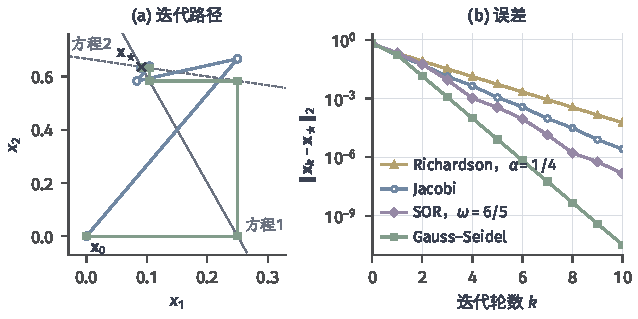
\includegraphics[width=108mm]{figures/01-basic-mathematics/03-vectors-matrices-and-multivariate-functions/matplotlib/c5-stationary-iteration-paths/figure.pdf}
  \caption{定常迭代在贯穿例$\bm A=\begin{bmatrix}4&1\\1&3\end{bmatrix}$，$\bm b=(1,2)^\top$，$\bm x_0=\bm 0$上的真实迭代值。左：实线与虚线分别是第一、第二个方程的解集，两者交于$\bm x_\star=(1/11,7/11)^\top$；蓝色圆点为Jacobi前四轮的迭代点，绿色折线为Gauss--Seidel前三轮的逐坐标路径。右：Richardson（$\alpha=1/4$）、Jacobi、SOR（$\omega=6/5$）与Gauss--Seidel的误差$\lVert\bm x_k-\bm x_\star\rVert_2$，纵轴取对数，渐近斜率分别对应谱半径约$0.40$、$0.29$、$0.20$与$1/12$。}
  \label{fig:ls-stationary-iteration-paths}
\end{figure}

\section{SOR迭代}
\label{sec:ls-sor}

Gauss--Seidel的每个分量修正都恰好让当前方程成立，修正幅度是固定的。\term{逐次超松弛迭代}（successive over-relaxation，SOR）引入固定的\term{松弛参数}（relaxation parameter）$\omega\neq0$，把每个分量的这一修正乘以$\omega$，目的是在误差沿同一方向缓慢衰减时走得更快，或在修正过冲时收敛得更稳。

这相当于把下三角修正矩阵的对角部分除以$\omega$，取$\bm M=\frac1\omega\bm D+\bm L$。$\omega=1$就是Gauss--Seidel；$0<\omega<1$称为欠松弛，只走一部分；$\omega>1$称为过松弛，越过Gauss--Seidel的修正继续走。松弛参数改变的是修正，目标方程没有变。

\paragraph{求修正量}
修正方程$\bigl(\frac1\omega\bm D+\bm L\bigr)\bm\delta_k=\bm r_k$按元素写出是
\[
 \begin{bmatrix}\frac{a_{1,1}}{\omega}&&&\\a_{2,1}&\frac{a_{2,2}}{\omega}&&\\\vdots&\vdots&\ddots&\\a_{d,1}&a_{d,2}&\cdots&\frac{a_{d,d}}{\omega}\end{bmatrix}
 \begin{bmatrix}(\bm\delta_k)_1\\(\bm\delta_k)_2\\\vdots\\(\bm\delta_k)_d\end{bmatrix}
 =\begin{bmatrix}(\bm r_k)_1\\(\bm r_k)_2\\\vdots\\(\bm r_k)_d\end{bmatrix},
\]
其中对角线以上的空白位置都是零。第$i$行的方程是
\[
 \sum_{j<i}a_{i,j}(\bm\delta_k)_j+\frac{a_{i,i}}{\omega}(\bm\delta_k)_i=(\bm r_k)_i\qquad(i=1,\ldots,d).
\]
两边乘以$\omega$，各行合起来就是$(\bm D+\omega\bm L)\bm\delta_k=\omega\bm r_k$，与上面的方程等价。系数矩阵仍是下三角矩阵，按前代求解。第一个方程只含$(\bm\delta_k)_1$，得
\[
 (\bm\delta_k)_1=\frac{\omega(\bm r_k)_1}{a_{1,1}} .
\]
第二个方程中$(\bm\delta_k)_1$已经求出，移项后得
\[
 (\bm\delta_k)_2=\frac{\omega}{a_{2,2}}\bigl((\bm r_k)_2-a_{2,1}(\bm\delta_k)_1\bigr) .
\]
一般地，把第$i$个方程中已经求出的前$i-1$个分量移到右边，再乘以$\omega/a_{i,i}$，得
\begin{equation}
 (\bm\delta_k)_i=\frac{\omega}{a_{i,i}}\Bigl((\bm r_k)_i-\sum_{j<i}a_{i,j}(\bm\delta_k)_j\Bigr)\qquad(i=1,\ldots,d).
 \label{eq:ls-sor-correction}
\end{equation}
括号里仍是前$i-1$个分量修正之后第$i$个方程的残差，除以$a_{i,i}$就是Gauss--Seidel在此刻给出的修正，SOR再把它乘以$\omega$。$\omega=1$时上式逐项退化为式~\eqref{eq:ls-gauss-seidel-correction}。前面的$(\bm\delta_k)_j$已经是松弛后的修正，所以SOR不等于先做一轮Gauss--Seidel再把整个修正量乘以$\omega$。

\paragraph{迭代公式}
把式~\eqref{eq:ls-sor-correction}加到当前近似上，得到第$i$个分量的新值
\begin{equation}
 \begin{aligned}
 (\bm x_{k+1})_i&=(\bm x_k)_i+\frac{\omega}{a_{i,i}}\Bigl((\bm r_k)_i-\sum_{j<i}a_{i,j}(\bm\delta_k)_j\Bigr),\\
 i&=1,\ldots,d,
 \end{aligned}
 \label{eq:ls-sor-update}
\end{equation}
写成向量形式是
\[
 \bm x_{k+1}=\bm x_k+\omega(\bm D+\omega\bm L)^{-1}\bm r_k .
\]

\subsection{算法实现}

输入是$\bm A$与$\bm b$，输出是近似解$\bm x$。除执行流程的参数外，还要预先选定松弛参数$\omega$和变量顺序，顺序固定为$1,\ldots,d$。停止检查与残差重算沿用第~\ref{sec:ls-matrix-splitting}节的流程，求修正量的一步换成带松弛参数的前代；与Gauss--Seidel一样，本轮的$\bm r_k$在整轮中保持不变。下面在例~\ref{ex:ls-stationary-running-example}上取$\omega=6/5$给出前两轮。
\begin{enumerate}
 \item \textbf{核对参数与对角元。}确认所有$a_{i,i}\neq0$。参数是否合格与矩阵是否满足假设是两项不同的检查：对称正定情形的收敛保证（定理~\ref{thm:ls-sor-convergence}）要求$0<\omega<2$，同时要求$\bm A$确实对称正定。

 例中$\bm A$对称正定，$\omega=6/5$在$(0,2)$内。

 \item \textbf{按顺序求修正量。}根据式~\eqref{eq:ls-sor-correction}，对$i=1,\ldots,d$依次计算$(\bm\delta_k)_i$。后面的行扣除的是前面已经松弛后的修正。

 例中第一轮的残差为$\bm r_0=\bm b=(1,2)^\top$：
 \[
  \begin{aligned}
  (\bm\delta_0)_1&=\frac{\omega}{a_{1,1}}(\bm r_0)_1=\frac{6/5}{4}\cdot1=\frac3{10},\\
  (\bm\delta_0)_2&=\frac{\omega}{a_{2,2}}\bigl((\bm r_0)_2-a_{2,1}(\bm\delta_0)_1\bigr)=\frac{6/5}{3}\Bigl(2-1\cdot\tfrac3{10}\Bigr)=\frac{17}{25} .
  \end{aligned}
 \]
 第二行扣除的是松弛后的$3/10$，而不是Gauss--Seidel的$1/4$。

 若先做完整一轮Gauss--Seidel，再把修正量乘以$\omega$，得到的是$\tfrac65(1/4,7/12)^\top=(3/10,7/10)^\top$，与$\bm\delta_0$不同；这一般是另一种方法，不是SOR。

 \item \textbf{更新并重算残差。}根据式~\eqref{eq:ls-sor-update}，令$(\bm x_{k+1})_i=(\bm x_k)_i+(\bm\delta_k)_i$，再按原方程重算残差。与Gauss--Seidel一样，也可以在一个向量上原位逐分量更新，处理第$i$行时现算这一行的残差。

 例中$\bm x_1=\bm x_0+\bm\delta_0=(3/10,17/25)^\top$，
 \[
  \begin{aligned}
  (\bm r_1)_1&=1-\bigl(4\cdot\tfrac3{10}+1\cdot\tfrac{17}{25}\bigr)=1-\tfrac{47}{25}=-\tfrac{22}{25},\\
  (\bm r_1)_2&=2-\bigl(1\cdot\tfrac3{10}+3\cdot\tfrac{17}{25}\bigr)=2-\tfrac{117}{50}=-\tfrac{17}{50} .
  \end{aligned}
 \]
 与第~\ref{sec:ls-gauss-seidel}节不同，第二个方程不再恰好成立，因为它的修正被放大了五分之一。

 \item \textbf{进入下一轮。}令$k\leftarrow k+1$，回到执行流程的停止检查；没有停止时重复第2、3步。

 例中$\lVert\bm r_1\rVert_2\approx0.94$，继续第二轮。用$\bm r_1=(-22/25,-17/50)^\top$求修正量：
 \[
  \begin{aligned}
  (\bm\delta_1)_1&=\frac{6/5}{4}\cdot\Bigl(-\frac{22}{25}\Bigr)=-\frac{33}{125},\\
  (\bm\delta_1)_2&=\frac{6/5}{3}\Bigl(-\frac{17}{50}-1\cdot\Bigl(-\frac{33}{125}\Bigr)\Bigr)\\
  &=\frac25\cdot\Bigl(-\frac{19}{250}\Bigr)=-\frac{19}{625},
  \end{aligned}
 \]
 于是
 \[
  \bm x_2=\bm x_1+\bm\delta_1=\begin{bmatrix}\tfrac3{10}-\tfrac{33}{125}\\\tfrac{17}{25}-\tfrac{19}{625}\end{bmatrix}=\begin{bmatrix}\tfrac9{250}\\\tfrac{406}{625}\end{bmatrix}.
 \]
 重算残差得
 \[
  \begin{aligned}
  (\bm r_2)_1&=1-\bigl(4\cdot\tfrac9{250}+1\cdot\tfrac{406}{625}\bigr)=\tfrac{129}{625},\\
  (\bm r_2)_2&=2-\bigl(1\cdot\tfrac9{250}+3\cdot\tfrac{406}{625}\bigr)=\tfrac{19}{1250} .
  \end{aligned}
 \]
\end{enumerate}

就这个例子而言，过松弛并没有带来好处：两轮的残差长度约为$0.94$与$0.21$，都大于Gauss--Seidel的$0.58$与$0.049$。有限轮的算例只用来解释计算过程；参数的优劣要由下面的谱半径判断。

\subsection{算法分析}

\paragraph{收敛条件}
由迭代公式的向量形式，SOR的修正矩阵满足$\bm M^{-1}=\omega(\bm D+\omega\bm L)^{-1}$，迭代矩阵为
\begin{equation}
\begin{aligned}
\bm T_\omega&=\bm I-\omega(\bm D+\omega\bm L)^{-1}\bm A\\
&=(\bm D+\omega\bm L)^{-1}\bigl[(1-\omega)\bm D-\omega\bm U\bigr],
\end{aligned}
 \label{eq:ls-sor-iteration-matrix}
\end{equation}
第二个等号用到$(\bm D+\omega\bm L)-\omega(\bm D+\bm L+\bm U)=(1-\omega)\bm D-\omega\bm U$。
$\omega$同时影响每个坐标的修正幅度与整轮的误差传播，所以不能随意取：它的取值范围对一般矩阵有一条必要条件，对实对称正定矩阵则恰好也是充分条件。
\begin{theorem}[SOR迭代的收敛条件]
\label{thm:ls-sor-convergence}
设$\bm A$的对角元全不为零。
\begin{enumerate}
\item 对任意这样的方阵，$\rho(\bm T_\omega)\geq|1-\omega|$；所以SOR对所有初值收敛的必要条件是$0<\omega<2$。
\item 若$\bm A$实对称正定且$0<\omega<2$，则$\rho(\bm T_\omega)<1$，SOR对所有初值收敛。
\end{enumerate}
\end{theorem}
\begin{proof}
（1）$\bm D+\omega\bm L$是下三角阵，行列式为$\prod_i a_{i,i}$；$(1-\omega)\bm D-\omega\bm U$是上三角阵，行列式为$(1-\omega)^d\prod_i a_{i,i}$。所以
\[
 \det\bm T_\omega=(1-\omega)^d .
\]
行列式等于全部特征值之积，其模不超过$\rho(\bm T_\omega)^d$，故$\rho(\bm T_\omega)\geq|1-\omega|$。若$\omega\leq0$或$\omega\geq2$，则$\rho(\bm T_\omega)\geq1$，由定理~\ref{thm:ls-stationary-convergence}不能对所有初值收敛。

（2）第$i$次坐标修正的步长是$t=\omega r_i/a_{i,i}$，代入定理~\ref{thm:ls-gauss-seidel-convergence}证明中的能量变化式，$\phi$减少
\[
\omega\frac{r_i^2}{a_{i,i}}-\frac{\omega^2}{2}\frac{r_i^2}{a_{i,i}}=\frac{\omega(2-\omega)\,r_i^2}{2a_{i,i}} .
\]
当$0<\omega<2$时这是非负量，且只在$r_i=0$时为零。此后的论证与该证明相同：一整轮能量不减少只能是$\bm e_k=\bm0$，于是$\bm A-\bm T_\omega^\top\bm A\bm T_\omega$正定，再由特征向量的二次型得$\rho(\bm T_\omega)<1$。
\end{proof}

\paragraph{参数选择与代价}
区间内收敛不等于每个参数都比Gauss--Seidel快。收敛速度取决于参数和变量排列：三对角等特殊结构的矩阵有由$\rho(\bm T_{\mathrm J})$给出的最优参数公式，但不能普遍套用。

贯穿例的$\omega=6/5$就使谱半径从Gauss--Seidel的$1/12$升到$0.2$。$\omega$接近区间端点时，由第一部分$\rho(\bm T_\omega)\geq|1-\omega|$接近一，收敛可能很弱。一轮成本与Gauss--Seidel同阶。

\section{SSOR迭代}
\label{sec:ls-ssor}

单向扫掠依赖变量顺序，对应的$\bm M=\bm D/\omega+\bm L$也不对称。对实对称正定的$\bm A$，\term{对称逐次超松弛迭代}（symmetric SOR，SSOR）把一次前向SOR扫掠与一次反向SOR扫掠配成一轮，参数取固定的$0<\omega<2$。

前向扫掠按$i=1,\ldots,d$的顺序做一次第~\ref{sec:ls-sor}节的SOR，得到中间近似$\bm x_{k+1/2}$；反向扫掠再按$i=d,\ldots,1$的顺序做一次SOR，每个坐标用后面的新值和前面的半步值，得到$\bm x_{k+1}$。

由对称性$\bm U=\bm L^\top$，记$\bm F=\bm D+\omega\bm L$，则$\bm F^\top=\bm D+\omega\bm U$。算法分析将证明，这两次扫掠合起来等价于取修正矩阵
\begin{equation}
 \bm M_{\mathrm{SSOR}}=\frac{1}{\omega(2-\omega)}\bm F\bm D^{-1}\bm F^\top .
 \label{eq:ls-ssor-correction-matrix}
\end{equation}
它是一个下三角、一个对角和一个上三角因子之积，修正方程可以逐个因子求解；它还对称正定，所以SSOR除了单独迭代，还能为第~\ref{chap:krylov-methods}章的共轭梯度法提供预条件。

\paragraph{求修正量}
修正方程$\bm M_{\mathrm{SSOR}}\bm\delta_k=\bm r_k$两边乘以$\omega(2-\omega)$，得
\[
 \bm F\bm D^{-1}\bm F^\top\bm\delta_k=\omega(2-\omega)\bm r_k .
\]
令$\bm z=\bm\delta_k/\bigl(\omega(2-\omega)\bigr)$，$\bm y=\bm D^{-1}\bm F^\top\bm z$，它拆成两个三角方程：先前代解$\bm F\bm y=\bm r_k$，再回代解$\bm F^\top\bm z=\bm D\bm y$，最后$\bm\delta_k=\omega(2-\omega)\bm z$。

下三角因子按元素写出是
\[
 \bm F=\begin{bmatrix}a_{1,1}&&&\\\omega a_{2,1}&a_{2,2}&&\\\vdots&\vdots&\ddots&\\\omega a_{d,1}&\omega a_{d,2}&\cdots&a_{d,d}\end{bmatrix},
\]
对角元取$\bm A$的对角元，严格下三角元乘以$\omega$，对角线以上都是零。$\bm F\bm y=\bm r_k$的第$i$行是
\[
 \omega\sum_{j<i}a_{i,j}y_j+a_{i,i}y_i=(\bm r_k)_i\qquad(i=1,\ldots,d).
\]
第一个方程只含$y_1$，得$y_1=(\bm r_k)_1/a_{1,1}$；此后第$i$个方程中$y_1,\ldots,y_{i-1}$已经求出，移项后除以$a_{i,i}$，得
\begin{equation}
 y_i=\frac{(\bm r_k)_i-\omega\sum_{j<i}a_{i,j}y_j}{a_{i,i}}\qquad(i=1,\ldots,d).
 \label{eq:ls-ssor-forward}
\end{equation}

上三角因子$\bm F^\top$的对角元仍是$a_{i,i}$，由对称性，它在$j>i$处的$(i,j)$元为$\omega a_{j,i}=\omega a_{i,j}$；右端$\bm D\bm y$的第$i$个分量是$a_{i,i}y_i$。所以$\bm F^\top\bm z=\bm D\bm y$的第$i$行是
\[
 a_{i,i}z_i+\omega\sum_{j>i}a_{i,j}z_j=a_{i,i}y_i\qquad(i=1,\ldots,d).
\]
这次最后一个方程只含$z_d$，得$z_d=y_d$；此后第$i$个方程中$z_{i+1},\ldots,z_d$已经求出，移项后除以$a_{i,i}$，得
\begin{equation}
 z_i=y_i-\frac{\omega}{a_{i,i}}\sum_{j>i}a_{i,j}z_j\qquad(i=d,d-1,\ldots,1).
 \label{eq:ls-ssor-backward}
\end{equation}
最后乘以常数，
\begin{equation}
 (\bm\delta_k)_i=\omega(2-\omega)z_i\qquad(i=1,\ldots,d).
 \label{eq:ls-ssor-correction}
\end{equation}

\paragraph{迭代公式}
把式~\eqref{eq:ls-ssor-correction}加到当前近似上，得到第$i$个分量的新值
\begin{equation}
 (\bm x_{k+1})_i=(\bm x_k)_i+\omega(2-\omega)z_i\qquad(i=1,\ldots,d),
 \label{eq:ls-ssor-update}
\end{equation}
其中$\bm z$由式~\eqref{eq:ls-ssor-forward}与式~\eqref{eq:ls-ssor-backward}依次求出。写成向量形式是
\[
 \bm x_{k+1}=\bm x_k+\omega(2-\omega)\bm F^{-\top}\bm D\bm F^{-1}\bm r_k .
\]

\subsection{算法实现}

输入是实对称正定的$\bm A$与$\bm b$，输出是近似解$\bm x$。除执行流程的参数外，还要预先选定$\omega$。停止检查与残差重算沿用第~\ref{sec:ls-matrix-splitting}节的流程，求修正量的一步换成一次前代与一次回代，内部多两个与$\bm x$同长的向量$\bm y$与$\bm z$。下面在例~\ref{ex:ls-stationary-running-example}上取$\omega=1$给出前两轮；这时$\bm F=\bm D+\bm L=\left[\begin{smallmatrix}4&0\\1&3\end{smallmatrix}\right]$，$\omega(2-\omega)=1$。
\begin{enumerate}
 \item \textbf{核对条件。}确认$\bm A$对称正定且$0<\omega<2$；正定矩阵的对角元都为正，所以各次除法都能执行。

 例中$\bm A$对称正定，$a_{1,1}=4$，$a_{2,2}=3$，$\omega=1$。

 \item \textbf{前代。}根据式~\eqref{eq:ls-ssor-forward}，对$i=1,\ldots,d$依次计算$y_i$，右端是本轮开始时的残差$\bm r_k$。

 例中第一轮的残差为$\bm r_0=\bm b=(1,2)^\top$：
 \[
  \begin{aligned}
  y_1&=\frac{(\bm r_0)_1}{a_{1,1}}=\frac14,\\
  y_2&=\frac{(\bm r_0)_2-\omega a_{2,1}y_1}{a_{2,2}}=\frac{2-1\cdot\tfrac14}{3}=\frac7{12} .
  \end{aligned}
 \]
 $\omega=1$时$\bm F=\bm D+\bm L$，$\bm y$就是Gauss--Seidel的修正量$\bm\delta_0$。

 \item \textbf{回代并缩放。}根据式~\eqref{eq:ls-ssor-backward}，对$i=d,\ldots,1$依次计算$z_i$，再按式~\eqref{eq:ls-ssor-correction}乘以$\omega(2-\omega)$得到$\bm\delta_k$。

 例中先处理第二行，再用刚得到的$z_2$处理第一行：
 \[
  \begin{aligned}
  z_2&=y_2=\frac7{12},\\
  z_1&=y_1-\frac{\omega}{a_{1,1}}a_{1,2}z_2=\frac14-\frac14\cdot\frac7{12}=\frac5{48},
  \end{aligned}
 \]
 所以$\bm\delta_0=\bm z=(5/48,7/12)^\top$。

 \item \textbf{更新并重算残差。}根据式~\eqref{eq:ls-ssor-update}，令$(\bm x_{k+1})_i=(\bm x_k)_i+(\bm\delta_k)_i$，再按原方程重算$\bm r_{k+1}=\bm b-\bm A\bm x_{k+1}$。

 例中$\bm x_1=\bm x_0+\bm\delta_0=(5/48,7/12)^\top$，
 \[
  \begin{aligned}
  (\bm r_1)_1&=1-\bigl(4\cdot\tfrac5{48}+1\cdot\tfrac7{12}\bigr)=0,\\
  (\bm r_1)_2&=2-\bigl(1\cdot\tfrac5{48}+3\cdot\tfrac7{12}\bigr)=\tfrac7{48} .
  \end{aligned}
 \]
 这次为零的是第一个分量，因为按双向扫掠来看，反向扫掠最后修正的是第一行。

 \item \textbf{进入下一轮。}令$k\leftarrow k+1$，回到执行流程的停止检查；没有停止时重复第2至4步。

 例中$\lVert\bm r_1\rVert_2=7/48\approx0.15$，继续第二轮。由$\bm r_1=(0,7/48)^\top$，前代与回代给出
 \[
  \begin{aligned}
  y_1&=\frac{0}{4}=0, & y_2&=\frac{\tfrac7{48}-1\cdot0}{3}=\frac7{144},\\
  z_2&=y_2=\frac7{144}, & z_1&=0-\frac14\cdot\frac7{144}=-\frac7{576},
  \end{aligned}
 \]
 于是
 \[
  \bm x_2=\bm x_1+\bm z=\begin{bmatrix}\tfrac5{48}-\tfrac7{576}\\\tfrac7{12}+\tfrac7{144}\end{bmatrix}=\begin{bmatrix}\tfrac{53}{576}\\\tfrac{91}{144}\end{bmatrix}.
 \]
 重算残差得
 \[
  \begin{aligned}
  (\bm r_2)_1&=1-\bigl(4\cdot\tfrac{53}{576}+1\cdot\tfrac{91}{144}\bigr)=0,\\
  (\bm r_2)_2&=2-\bigl(1\cdot\tfrac{53}{576}+3\cdot\tfrac{91}{144}\bigr)=\tfrac7{576} .
  \end{aligned}
 \]
 两轮中各个三角子问题都精确解出了，残差却仍不为零。验收用的是原方程的残差，不能以子问题已经解完代替。
\end{enumerate}

\paragraph{双向扫掠}
等价的实现按本节开头的描述做两次SOR扫掠，代替上面的第2、3步。前向扫掠按式~\eqref{eq:ls-sor-correction}由$\bm r_k$求出修正量$\bm\delta_{\mathrm f}$，令$\bm x_{k+1/2}=\bm x_k+\bm\delta_{\mathrm f}$，再按原方程算出半步后的残差$\bm r_{k+1/2}=\bm b-\bm A\bm x_{k+1/2}$。

反向扫掠按$i=d,\ldots,1$的顺序求
\begin{equation}
 (\bm\delta_{\mathrm b})_i=\frac{\omega}{a_{i,i}}\Bigl((\bm r_{k+1/2})_i-\sum_{j>i}a_{i,j}(\bm\delta_{\mathrm b})_j\Bigr),
 \label{eq:ls-ssor-backward-sweep}
\end{equation}
令$\bm x_{k+1}=\bm x_{k+1/2}+\bm\delta_{\mathrm b}$。反向扫掠的右端必须是半步后的残差，不能继续使用本轮开始时的$\bm r_k$。

两次扫掠也都可以在同一个向量上原位逐坐标更新，每行的残差在访问时现算，不必单独形成$\bm r_{k+1/2}$。算法分析中的推导说明，两次修正之和正是式~\eqref{eq:ls-ssor-correction}给出的$\bm\delta_k$。

例中第一轮的前向扫掠就是一轮Gauss--Seidel，给出
\[
 \bm\delta_{\mathrm f}=\bm x_{1/2}=\begin{bmatrix}1/4\\7/12\end{bmatrix},\qquad
 \bm r_{1/2}=\begin{bmatrix}-7/12\\0\end{bmatrix}.
\]
反向扫掠先处理第二行，再处理第一行：
\[
 (\bm\delta_{\mathrm b})_2=\frac{0}{3}=0,\qquad
 (\bm\delta_{\mathrm b})_1=\frac{-\tfrac7{12}-1\cdot0}{4}=-\frac7{48},
\]
所以$\bm x_1=(1/4-7/48,\,7/12)^\top=(5/48,7/12)^\top$，与因子求解一致。第二分量保持不变，因为前向扫掠的最后一步已经让第二个方程成立。

\paragraph{作为预条件}
作为共轭梯度法的预条件使用时，SSOR不更新近似解，只把外层迭代给出的残差$\bm r$变成修正方向：以$\bm r$代替$\bm r_k$，按式~\eqref{eq:ls-ssor-forward}、式~\eqref{eq:ls-ssor-backward}前代、回代并缩放，返回$\bm M_{\mathrm{SSOR}}^{-1}\bm r$，近似解由外层方法另行更新。同一次外层求解中，$\omega$和三角因子要保持不变，否则预条件矩阵逐轮变化，外层方法依赖的固定内积结构就不成立。具体用法见第~\ref{sec:ls-preconditioning}节。

\subsection{算法分析}

\paragraph{修正矩阵}
先把两次扫掠的修正合并成一个修正矩阵，并确定缩放常数，使独立迭代与作为预条件的实现使用同一约定。

前向半步就是一次SOR：解$\bm F\bm\delta_{\mathrm f}=\omega\bm r_k$，令$\bm x_{k+1/2}=\bm x_k+\bm\delta_{\mathrm f}$。

反向半步按$i=d,\ldots,1$的顺序做SOR，先访问的是下标大的分量，所以本轮新值出现在上三角部分，对应的方程是$\bm F^\top\bm\delta_{\mathrm b}=\omega\bm r_{k+1/2}$，再令$\bm x_{k+1}=\bm x_{k+1/2}+\bm\delta_{\mathrm b}$。右端是半步后的残差
\[
\bm r_{k+1/2}=\bm b-\bm A\bm x_{k+1/2}=\bm r_k-\bm A\bm\delta_{\mathrm f}.
\]

把两次修正相加。由$\bm\delta_{\mathrm f}=\omega\bm F^{-1}\bm r_k$，
\[
\begin{aligned}
\bm\delta_{\mathrm f}+\bm\delta_{\mathrm b}
&=\omega\bm F^{-1}\bm r_k+\omega\bm F^{-\top}\bigl(\bm r_k-\omega\bm A\bm F^{-1}\bm r_k\bigr)\\
&=\omega\bm F^{-\top}\bigl(\bm F^\top\bm F^{-1}+\bm F\bm F^{-1}-\omega\bm A\bm F^{-1}\bigr)\bm r_k\\
&=\omega\bm F^{-\top}\bigl(\bm F^\top+\bm F-\omega\bm A\bigr)\bm F^{-1}\bm r_k ,
\end{aligned}
\]
第二个等号在第一项前插入$\bm F^{-\top}\bm F^\top$，在第二项中插入$\bm F\bm F^{-1}$。又由$\bm F=\bm D+\omega\bm L$与$\bm F^\top=\bm D+\omega\bm U$，
\[
\begin{aligned}
\bm F^\top+\bm F-\omega\bm A
&=2\bm D+\omega(\bm L+\bm U)-\omega(\bm D+\bm L+\bm U)\\
&=(2-\omega)\bm D ,
\end{aligned}
\]
所以一整轮的修正为
\begin{equation}
\bm\delta_k=\omega(2-\omega)\,\bm F^{-\top}\bm D\bm F^{-1}\bm r_k ,
 \label{eq:ls-ssor-combined-correction}
\end{equation}
即$\bm M_{\mathrm{SSOR}}\bm\delta_k=\bm r_k$，$\bm M_{\mathrm{SSOR}}$就是本节开头给出的矩阵。

求解的次序是先解$\bm F$、再乘$\bm D$、最后解$\bm F^\top$，不必显式形成$\bm M_{\mathrm{SSOR}}$或它的逆；算法实现的第2、3步正是按这个次序。

这个修正矩阵对称正定。对称性由形式$\bm F\bm D^{-1}\bm F^\top$直接看出。$\bm A$正定，把第$i$个坐标单位向量代入二次型即得$a_{i,i}>0$，所以$\bm D\succ0$；$\bm F$是对角元为正的下三角阵，可逆。于是对$\bm v\neq\bm0$，
\[
\bm v^\top\bm M_{\mathrm{SSOR}}\bm v=\frac{(\bm F^\top\bm v)^\top\bm D^{-1}(\bm F^\top\bm v)}{\omega(2-\omega)}>0 ,
\]
这里用到$0<\omega<2$使分母为正。注意对称正定的是修正矩阵$\bm M_{\mathrm{SSOR}}$；迭代矩阵$\bm I-\bm M_{\mathrm{SSOR}}^{-1}\bm A$一般不是对称矩阵。

\paragraph{收敛性}
$\bm M_{\mathrm{SSOR}}$正定本身还不足以断言定常迭代收敛；还需要它在二次型意义下不小于$\bm A$。先展开
\[
 \bm F\bm D^{-1}\bm F^\top=\bm D+\omega\bm L+\omega\bm U+\omega^2\bm L\bm D^{-1}\bm U ,
\]
再减去$\omega(2-\omega)\bm A=\omega(2-\omega)(\bm D+\bm L+\bm U)$，整理得
\[
\begin{aligned}
\omega(2-\omega)(\bm M_{\mathrm{SSOR}}-\bm A)
&=(1-\omega)^2\bm D-\omega(1-\omega)(\bm L+\bm U)+\omega^2\bm L\bm D^{-1}\bm U\\
&=\bm C\bm D^{-1}\bm C^\top ,
\end{aligned}
\]
其中$\bm C=(1-\omega)\bm D-\omega\bm L$，最后一步把$\bm C\bm D^{-1}\bm C^\top$展开即可核对。因为$\bm D\succ0$，$\bm C\bm D^{-1}\bm C^\top\succeq0$，所以
\begin{equation}
\bm 0\prec\bm A\preceq\bm M_{\mathrm{SSOR}} .
 \label{eq:ls-ssor-dominates}
\end{equation}

由此读出迭代矩阵的谱。$\bm M_{\mathrm{SSOR}}$对称正定，有正定平方根（第~\ref{sec:ls-matrix-square-root}节）。令$\bm S=\bm M_{\mathrm{SSOR}}^{-1/2}\bm A\bm M_{\mathrm{SSOR}}^{-1/2}$，它实对称。若$\bm S\bm w=\mu\bm w$，$\bm w\neq\bm0$，令$\bm y=\bm M_{\mathrm{SSOR}}^{-1/2}\bm w$，则
\[
\mu=\frac{\bm w^\top\bm S\bm w}{\bm w^\top\bm w}=\frac{\bm y^\top\bm A\bm y}{\bm y^\top\bm M_{\mathrm{SSOR}}\bm y}\in(0,1].
\]
迭代矩阵可以写成
\[
 \bm T_{\mathrm{SSOR}}=\bm I-\bm M_{\mathrm{SSOR}}^{-1}\bm A=\bm M_{\mathrm{SSOR}}^{-1/2}(\bm I-\bm S)\bm M_{\mathrm{SSOR}}^{1/2} ,
\]
它与实对称矩阵$\bm I-\bm S$相似，特征值$1-\mu$全部落在$[0,1)$中，所以$\rho(\bm T_{\mathrm{SSOR}})<1$。

由定理~\ref{thm:ls-stationary-convergence}，在$\bm A$实对称正定、$0<\omega<2$时SSOR对所有初值收敛。这里$\bm T_{\mathrm{SSOR}}$本身一般不对称，只是相似于对称矩阵，因而特征值为实数。

\paragraph{代价与用途}
一轮含两次三角扫掠（或等价的前代、对角缩放与回代），另加一次计算残差的矩阵乘向量，工作量约为SOR一轮的两倍；存储只多一个与$\bm x$同长的中间向量。

比较时不能只数轮数：贯穿例中$\omega=1$的SSOR谱半径为$1/12$，与Gauss--Seidel相同，每轮却多花一倍计算。SSOR作为独立迭代往往并不比SOR省；它的主要价值在于对称正定的修正矩阵：作为预条件时，每次外层迭代多付两次三角求解，换来外层共轭梯度法所需步数的减少，是否划算要按总成本比较（第~\ref{sec:ls-preconditioning}节）。

\section{收敛检验与停止准则}
\label{sec:ls-stationary-stopping}

各方法都使用第~\ref{sec:ls-matrix-splitting}节的终止条件：$\lVert\bm r_k\rVert_2\leq\mathrm{atol}+\mathrm{rtol}\lVert\bm b\rVert_2$，或$k=K$。前者表示达到了给定的残差要求；后者只表示不再继续计算，结果未必达到精度。两种情况下输出都只是当前的$\bm x_k$，所以结束状态必须一并报告。残差用真实的$\bm b-\bm A\bm x_k$计算，而不是只依赖递推值。

几种量不能代替原方程的残差检验。修正量$\lVert\bm\delta_k\rVert$很小，可能只说明收缩因子接近一、迭代走得很慢，而不是已经接近解。残差在很多轮内几乎不降，应作为停滞报告，而不是当作收敛。计算中出现溢出或非数，应作为数值异常报告；这通常说明迭代发散或对角元过小。

残差小也不等于解的误差小。由$\bm x_\star-\bm x_k=\bm A^{-1}\bm r_k$，误差是残差经$\bm A^{-1}$放大的结果，两者之间隔着问题本身的敏感性；第~\ref{sec:ls-numerical-sensitivity}节再给出误差界和后向误差的解释。

比较不同方法时，应在相同精度要求下比较总工作量，而不是轮数；分析中的收敛率和代价用于解释算法，不加入求解器的输出。其他用递推方式维护残差的方法，递推值会因舍入而偏离真实残差，停止前也须用$\bm b-\bm A\bm x_k$复核。

\FloatBarrier
\section{本章小结}
\label{sec:stationary-iterations-summary}

本章回答了怎样不分解$\bm A$而逐步求解可逆方程$\bm A\bm x=\bm b$。共同的做法是矩阵分裂$\bm A=\bm M-\bm N$：每轮解一个以易解矩阵$\bm M$为系数的修正方程$\bm M\bm\delta_k=\bm r_k$，再更新近似解。误差满足$\bm e_{k+1}=(\bm I-\bm M^{-1}\bm A)\bm e_k$，由第~\ref{chap:linear-recurrence-stability}章的矩阵幂结论，迭代对任意初值收敛当且仅当迭代矩阵的谱半径小于一，渐近速度也由谱半径决定。

五种方法的区别只在于$\bm M$怎样近似$\bm A$、数据怎样读取。Richardson取$\bm M=\alpha^{-1}\bm I$，只需矩阵乘向量；对称正定时收敛当且仅当$0<\alpha<2/\lambda_{\max}$，最优步长的收缩因子为$(\kappa_2-1)/(\kappa_2+1)$。Jacobi取$\bm M=\bm D$，各分量只读旧值、可以并行，严格行对角占优保证收敛，对称正定本身不保证。

Gauss--Seidel取$\bm M=\bm D+\bm L$，立即使用本轮新值，相当于一次前代；严格行对角占优或对称正定都保证收敛。SOR取$\bm M=\bm D/\omega+\bm L$，$0<\omega<2$对一般矩阵是必要条件，对对称正定矩阵也是充分条件；区间内不同参数的速度仍须比较。SSOR把前向与反向SOR配成一轮，修正矩阵$\bm M_{\mathrm{SSOR}}=\bm F\bm D^{-1}\bm F^\top/[\omega(2-\omega)]$对称正定且满足$\bm A\preceq\bm M_{\mathrm{SSOR}}$，由此证明收敛，并可作为共轭梯度法的预条件。

这些结论都有边界。对角元非零只保证可执行，不保证收敛；用了新信息、加了过松弛，都不自动更快；贯穿例中Gauss--Seidel的谱半径为$1/12$，$\omega=6/5$的SOR反而是$0.2$。比较方法要把谱半径决定的轮数与每轮成本合起来，看达到相同精度的总工作量。

停止计算也要分清含义。只有真实残差满足$\lVert\bm r_k\rVert_2\leq\mathrm{atol}+\mathrm{rtol}\lVert\bm b\rVert_2$才算达到残差目标；步数耗尽、停滞或数值异常都只是停止，修正量很小也不代表接近解。即使残差达标，前向误差仍受问题条件数制约，这在第~\ref{sec:ls-numerical-sensitivity}节讨论；第~\ref{chap:krylov-methods}章则在逐步扩大的子空间中选择近似，以改善定常迭代受谱半径限制的收敛速度。

% Krylov子空间法：Krylov子空间、Arnoldi正交化、Lanczos过程、Golub--Kahan双对角化、MINRES、CG、GMRES、BiCG、BiCGSTAB、LSQR、LSMR与预条件
\chapter{Krylov子空间法}
\label{sec:ls-krylov-iterations}
\label{chap:krylov-methods}

第~\ref{chap:stationary-iterations}章的定常迭代每轮按同一个规则修正近似解：算出残差$\bm r_k$，解一次$\bm M\bm\delta_k=\bm r_k$，加到$\bm x_k$上。这一轮的残差用完就被丢弃，下一轮只看到新的近似。可是$\bm r_0,\bm r_1,\ldots$以及它们被$\bm A$作用后的向量都携带着关于解的信息；只用最新的一个，等于每轮放弃了此前积累的全部方向。

本章的方法把这些向量张成的子空间保留下来，每轮在逐步扩大的子空间中按某个准则重新选择近似。由此产生三个问题：怎样以数值上可靠的方式生成子空间的基；在子空间中按什么准则选解，这个准则对矩阵提出什么要求；以及怎样只用固定数量的向量完成计算，而不让存储随步数增长。

各节先建立生成子空间基的工具，再给出使用这些基的求解方法。第~\ref{sec:ls-krylov-subspaces}节建立Krylov子空间及其与残差多项式的对应，并比较在子空间中选解的几种准则。

随后三节给出生成基的过程。Arnoldi正交化从一般方阵说起，把$\bm A\bm v_j$与全部已有基向量正交化，得到标准正交基，并把$\bm A$压缩成上Hessenberg小矩阵，原方程由此化为小型方程组或小型最小二乘问题；Lanczos过程是它在对称矩阵上的简化，正交化只剩三项递推，小矩阵成为对称三对角矩阵；长方或秩亏的最小二乘问题中，残差与未知量不在同一个空间，Golub--Kahan双对角化交替作用$\bm A$与$\bm A^\top$，在两个空间中各生成一组标准正交基，把$\bm A$压缩成下双对角小矩阵。

此后各节展开求解方法：MINRES借Lanczos过程对对称（可以不定）矩阵使原残差最小；对称正定矩阵还可用共轭梯度法，使误差的能量范数最小，它利用三对角矩阵的分解把递推压缩到只需上一步的信息；GMRES借Arnoldi正交化对一般方阵同样使原残差最小，代价是基的存储随步数增长；非对称矩阵若要固定存储，可放弃残差最小化，BiCG借转置矩阵维持双正交关系，BiCGSTAB再用局部的残差平滑取代转置乘法；LSQR与LSMR借Golub--Kahan双对角化，分别使原残差与正规残差最小。

这三个生成基的过程是求解方法共用的底层子空间工具，只给出基与压缩后的小矩阵，不作为方程求解的输出；它们集中放在所有求解方法之前，读到求解方法时，所需的基与小矩阵关系都已建立。最后一节讨论所有方法共用的预条件：用接近$\bm A$而又易解的矩阵改善迭代面对的谱分布，并说明它以左预条件、右预条件或预条件共轭梯度法的形式嵌入求解器。各求解方法的停止判断沿用第~\ref{sec:ls-stationary-stopping}节的规则，以真实残差为准。

这些方法依赖前面几章的结论。第~\ref{chap:linear-solution-selection}章给出正规方程、最小范数解与加权最小二乘；第~\ref{chap:direct-least-squares-solvers}章给出修正Gram--Schmidt与Givens旋转，第~\ref{chap:direct-linear-solvers}章给出三角代入以及LU与Cholesky的消元公式；收敛界用到第~\ref{chap:eigen-spectral-decomposition}章的实对称谱定理；停止准则、贯穿例与SSOR分裂沿用第~\ref{chap:stationary-iterations}章。需要注意，Krylov方法每轮的步长和组合系数都由当前向量算出，迭代不是同一个线性映射的反复作用，所以第~\ref{chap:linear-recurrence-stability}章关于固定误差矩阵的谱半径判据不能直接套用；收敛性要从各方法自己的选解准则推出。

记号沿用前几章：方阵情形$\bm A\in\mathbb R^{d\times d}$，最小二乘情形$\bm A\in\mathbb R^{m\times d}$；精确解记作$\bm x_\star$，最小二乘解记作$\hat{\bm x}$，迭代近似记作$\bm x_k$，残差记作$\bm r_k=\bm b-\bm A\bm x_k$。

三个生成基的过程都按主要思想、计算过程、算法分析、应用四部分展开，算法分析说明$\bm A$被压缩成怎样的小矩阵，应用说明小矩阵怎样用于求解方程；每种求解方法从相应工具的应用出发，先在主要思想中推出怎样求解子空间中的小问题，再在算法实现中写出变量、初始化与每轮更新，并结合贯穿例给出数值，最后在算法分析中说明正确性与收敛性。

\section{Krylov子空间}
\label{sec:ls-krylov-subspaces}

本章各方法都在同一类子空间中寻找近似解。本节先给出这类子空间的定义，说明在其中取近似等价于选择一个残差多项式；再从$\bm A$的谱把“残差尽量小”转化为寻找多项式的问题；最后讨论怎样选择这个多项式，并由此看出与定常迭代的区别和本章各方法的选择策略。

\subsection{Krylov子空间与残差多项式}

设$\bm A\in\mathbb R^{d\times d}$可逆，初值为$\bm x_0$，初始残差为$\bm r_0=\bm b-\bm A\bm x_0$。由$\bm A\bm x_\star=\bm b$得$\bm A(\bm x_\star-\bm x_0)=\bm r_0$，即
\[
 \bm x_\star-\bm x_0=\bm A^{-1}\bm r_0 .
\]
所需的修正量由$\bm r_0$经$\bm A^{-1}$作用得到。$\bm A^{-1}$无法直接使用，但$\bm A$与向量的乘积容易计算。从$\bm r_0$出发反复乘以$\bm A$，所得向量张成的子空间
\begin{equation}
 \mathcal K_k(\bm A,\bm r_0)=\operatorname{span}\{\bm r_0,\bm A\bm r_0,\ldots,\bm A^{k-1}\bm r_0\}
 \label{eq:ls-krylov-subspace}
\end{equation}
称为第$k$个\term{Krylov子空间}（Krylov subspace），不致混淆时简记为$\mathcal K_k$。

Krylov子空间法在第$k$步把近似解取在仿射集合$\bm x_0+\mathcal K_k$中。每增加一个基向量，只需把上一个向量再乘一次$\bm A$，不必形成矩阵的幂。

这一限制的意义在于，它把求解方程转化为选择一个多项式。若$\bm x_k\in\bm x_0+\mathcal K_k$，则$\bm x_k-\bm x_0$是$\bm r_0,\bm A\bm r_0,\ldots,\bm A^{k-1}\bm r_0$的线性组合，可写成
\[
 \bm x_k=\bm x_0+q_{k-1}(\bm A)\bm r_0 ,
\]
其中$q_{k-1}$是次数不超过$k-1$的多项式。相应的残差为
\[
 \bm r_k=\bm b-\bm A\bm x_0-\bm A\,q_{k-1}(\bm A)\bm r_0=\bigl(\bm I-\bm A\,q_{k-1}(\bm A)\bigr)\bm r_0 .
\]
令$p_k(t)=1-t\,q_{k-1}(t)$，则$p_k$的次数不超过$k$，且$p_k(0)=1$，残差可写成
\[
 \bm r_k=p_k(\bm A)\bm r_0 .
\]
条件$p_k(0)=1$反映近似解总是$\bm x_0$加上一个修正：零次多项式$p_0=1$对应不作修正，残差保持为$\bm r_0$。

下面的引理说明，这一对应在两个方向上都成立。

\begin{lemma}[Krylov残差多项式]
\label{lem:ls-krylov-residual-polynomial}
记$\mathcal P_k=\{p:\deg p\le k,\ p(0)=1\}$。若$\bm x_k\in\bm x_0+\mathcal K_k$，则存在$p_k\in\mathcal P_k$，使
\begin{equation}
 \label{eq:ls-krylov-residual-polynomial}
 \bm r_k=\bm b-\bm A\bm x_k=p_k(\bm A)\bm r_0 ;
\end{equation}
反之，对每个$p_k\in\mathcal P_k$，$\bm x_0+\mathcal K_k$中都有一个近似解，其残差为$p_k(\bm A)\bm r_0$。
\end{lemma}

\begin{proof}
正向由上面的计算给出。反之，若$p_k\in\mathcal P_k$，则$1-p_k(t)$在$t=0$处为零，可写成$t\,q_{k-1}(t)$，其中$\deg q_{k-1}\le k-1$；取$\bm x=\bm x_0+q_{k-1}(\bm A)\bm r_0\in\bm x_0+\mathcal K_k$，其残差为$\bm r_0-\bm A\,q_{k-1}(\bm A)\bm r_0=p_k(\bm A)\bm r_0$。
\end{proof}
因此，在$\bm x_0+\mathcal K_k$中选取近似解，与在$\mathcal P_k$中选取残差多项式是同一件事。

\subsection{残差多项式的目标}

上一小节说明，$\bm x_0+\mathcal K_k$中的每个近似$\bm x_k$都对应一个残差多项式$p_k\in\mathcal P_k$，残差为$\bm r_k=p_k(\bm A)\bm r_0$，选不同的近似就是选不同的$p_k$。本小节说明，对固定的一轮$k$，希望选出的$p_k$应当满足什么要求，才能使残差尽量小。下文中，$p$泛指任意多项式，$p_k$专指第$k$步近似所对应的那一个。

\paragraph{残差多项式在特征方向上的分解}
先说明矩阵多项式的含义。对多项式$p(t)=\mu_0+\mu_1t+\cdots+\mu_mt^m$，把变量$t$换成矩阵$\bm A$、常数项换成$\mu_0\bm I$，得到矩阵
\[
  p(\bm A)=\mu_0\bm I+\mu_1\bm A+\cdots+\mu_m\bm A^m .
\]
例如$p_1(t)=1-ct$时，$p_1(\bm A)=\bm I-c\bm A$。

设$\bm v$是$\bm A$的一个特征向量，对应的特征值为$\lambda$，即$\bm A\bm v=\lambda\bm v$，$\bm v\ne\bm0$。反复使用这一关系得$\bm A^j\bm v=\lambda^j\bm v$，代入$p(\bm A)$的各项，
\begin{equation}
 p(\bm A)\bm v=\mu_0\bm v+\mu_1\lambda\bm v+\cdots+\mu_m\lambda^m\bm v=p(\lambda)\,\bm v .
 \label{eq:ls-krylov-polynomial-eigenvector}
\end{equation}
矩阵多项式作用在特征向量上，只是把它乘以多项式在相应特征值处的值。

再设$\bm A$可对角化，它的特征向量$\bm v_1,\ldots,\bm v_d$组成一组基，对应的特征值为$\lambda_1,\ldots,\lambda_d$。把初始残差按这组基展开
\[
  \bm r_0=\sum_{i=1}^d\xi_i\bm v_i ,
\]
$\xi_i$是$\bm r_0$在第$i$个特征方向上的坐标。

对每一项使用上式，得
\begin{equation}
 \bm r_k=p_k(\bm A)\bm r_0=\sum_{i=1}^d\xi_i\,p_k(\lambda_i)\,\bm v_i .
 \label{eq:ls-krylov-residual-eigen-expansion}
\end{equation}

初始残差在第$i$个特征方向上的分量$\xi_i$，到第$k$步变为$\xi_i\,p_k(\lambda_i)$。各个方向互不干扰：$|p_k(\lambda_i)|$小，这个方向上的残差就被压小；$p_k(\lambda_i)=0$，这个方向上的残差就被完全消去。

\paragraph{目标残差多项式}
于是，让第$k$步的残差尽量小，就变成了一个关于实数多项式的问题：找一个次数不超过$k$的多项式$p_k$，使
\begin{equation}
 p_k(0)=1,\qquad\text{且}\qquad |p_k(\lambda_i)|\ \text{对每个特征值}\ \lambda_i\ \text{都尽量小}.
 \label{eq:ls-krylov-polynomial-target}
\end{equation}
若没有$p_k(0)=1$，取$p_k=0$就把残差全部消去；正是这个条件使问题不平凡：多项式在原点必须取值为一，在各特征值处却要接近零。

由此可以得到Krylov子空间法所需迭代次数的上限。设$\bm A$只有$m$个互不相同的特征值$\lambda_1,\ldots,\lambda_m$。次数为$m$的多项式
\begin{equation}
 p_m(t)=\Bigl(1-\frac{t}{\lambda_1}\Bigr)\cdots\Bigl(1-\frac{t}{\lambda_m}\Bigr)
 \label{eq:ls-krylov-annihilating-polynomial}
\end{equation}
满足$p_m(0)=1$，并在所有特征值处为零，所以第$m$步的残差可以为零；而次数低于$m$的非零多项式不可能在$m$个不同的点处都为零。因此，按最优准则选取多项式的Krylov子空间法，在精确算术下至多$m$步就得到精确解，最大迭代次数就是$\bm A$的不同特征值的个数$m$，它不超过维数$d$。

特征值越少、越集中，越容易用低次多项式在它们附近同时取到很小的值，实际所需的步数也越少；反过来，靠近原点的特征值最难处理，因为多项式要从原点处的$1$很快降到接近零。浮点计算中正交性会逐渐丧失，实际计算依据残差判断何时停止。

\subsection{残差多项式的选择策略}
\label{sec:ls-krylov-selection-criteria}

上一小节给出了目标，本小节讨论每一步怎样实际选出$p_k$。

\paragraph{定常迭代法：由$p_k$得到$p_{k+1}$}
第~\ref{chap:stationary-iterations}章的定常迭代，近似解实际上也落在Krylov子空间中，只是残差多项式的确定方式很死板。

以Richardson迭代为例，由$\bm r_{k+1}=(\bm I-\alpha\bm A)\bm r_k$得
\begin{equation}
 p_{k+1}(t)=(1-\alpha t)\,p_k(t),\qquad p_k(t)=(1-\alpha t)^k .
 \label{eq:ls-krylov-richardson-polynomial}
\end{equation}
下一步的多项式总是上一步的乘以同一个一次因子，根始终是$1/\alpha$，在迭代开始前就由步长固定了。

它在各特征值处是否足够小，只能由谱半径$\rho(\bm I-\alpha\bm A)$判断；当$\rho\geq1$时，迭代发散。一般的矩阵分裂迭代与此类似，多项式由迭代矩阵$\bm T$的幂确定。

\paragraph{Krylov子空间法：每一步重新选择}
Krylov子空间法更灵活：第$k$步直接在整个$\mathcal P_k$中选择$p_k$，不要求它由$p_{k-1}$乘一个因子得到。

由于$\mathcal P_{k-1}\subseteq\mathcal P_k$，上一步的多项式仍是可选的候选，所以按最优准则选取时，下一步的结果不会比上一步差；而新选出的$p_k$可以与$p_{k-1}$完全不同。

为了在整个子空间中选择，方法要保留此前各步得到的方向信息，这正是第~\ref{sec:ls-arnoldi}—\ref{sec:ls-bidiagonal-iteration}节生成标准正交基的过程所提供的。

\paragraph{贯穿例}
以例~\ref{ex:ls-stationary-running-example}为例，$\bm x_0=\bm 0$，$\bm r_0=\bm b=(1,2)^\top$，$\bm A$的两个特征值为
\[
 \lambda_1=\frac{7+\sqrt5}{2}\approx4.618,\qquad \lambda_2=\frac{7-\sqrt5}{2}\approx2.382 ,
\]
它们满足$\lambda_1+\lambda_2=7$，$\lambda_1\lambda_2=11$。

第一步的候选集合$\bm x_0+\mathcal K_1$是$\bm r_0$所在的直线，近似只能是$\bm x_1=c\,\bm r_0$，实数$c$是唯一可选的系数，残差为$\bm r_1=(\bm I-c\bm A)\bm r_0$，对应$p_1(t)=1-ct$。一次多项式只有一个根，不能同时在两个特征值处为零。

Richardson迭代取$c=\alpha=1/4$，两个特征方向上的因子为
\[
 p_1(\lambda_1)\approx-0.15,\qquad p_1(\lambda_2)\approx0.40 ;
\]
若改取$c=2/(\lambda_1+\lambda_2)=2/7$，两个值大小相等、符号相反，约为$\mp0.32$，最大的那个更小。可见即使在第一步，$c$也可以按某种准则选得更好。

第二步的候选集合是$\bm x_0+\mathcal K_2$。由
\[
 \det\begin{bmatrix}\bm r_0&\bm A\bm r_0\end{bmatrix}=\det\begin{bmatrix}1&6\\2&7\end{bmatrix}=-5\neq0
\]
知$\mathcal K_2=\mathbb R^2$，近似写成$\bm x_2=c_0\bm r_0+c_1\bm A\bm r_0$，对应
\[
  p_2(t)=1-c_0t-c_1t^2 .
\]

Richardson迭代只能把上一步的多项式再乘以$1-t/4$，
\[
 p_2(t)=\Bigl(1-\frac t4\Bigr)^2,\qquad p_2(\lambda_1)\approx0.024,\qquad p_2(\lambda_2)\approx0.16 ,
\]
残差仍不为零。

Krylov子空间法则在整个$\mathcal P_2$中重新选择，可以取以两个特征值为根的多项式
\[
 p_2(t)=\Bigl(1-\frac{t}{\lambda_1}\Bigr)\Bigl(1-\frac{t}{\lambda_2}\Bigr)=1-\frac{7}{11}t+\frac1{11}t^2 ,
\]
即$c_0=7/11$，$c_1=-1/11$。这时$\bm r_2=\bm0$，近似
\[
 \bm x_2=\frac7{11}\begin{bmatrix}1\\2\end{bmatrix}-\frac1{11}\begin{bmatrix}6\\7\end{bmatrix}=\begin{bmatrix}\tfrac1{11}\\\tfrac7{11}\end{bmatrix}
\]
正是精确解。这个$p_2$并不是第一步的$p_1$乘以某个因子，而是在更大的集合中重新选出的。

图~\ref{fig:solver-krylov-polynomial-roots}只比较两种二次多项式在同一谱上的取值。使谱点成为根能够消去对应特征分量，而重复固定因子一般做不到这一点。

\begin{figure}[!htb]
  \centering
  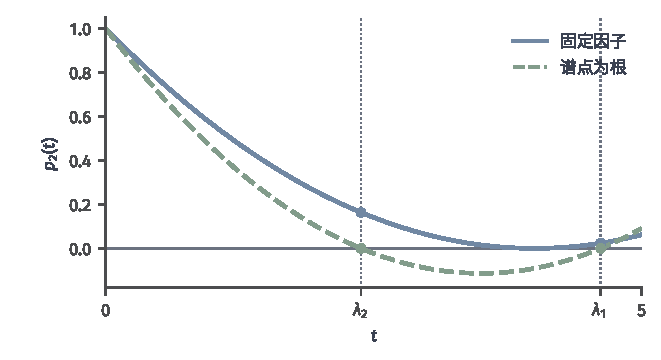
\includegraphics{figures/02-vectors-matrices-and-multivariate-calculus/03-linear-equations-and-optimization/matplotlib/learning-mechanisms/krylov-polynomial-roots.pdf}
  \caption{贯穿例$\bm A=\left[\begin{smallmatrix}4&1\\1&3\end{smallmatrix}\right]$的残差多项式。蓝线为Richardson两步的$(1-t/4)^2$，绿虚线为$1-7t/11+t^2/11$；圆点标记两个特征值处的值。二者均满足$p_2(0)=1$，只有后者在两个谱点同时为零。这是解释多项式自由度的解析对照，实际算法不需要预先知道特征值。}
  \label{fig:solver-krylov-polynomial-roots}
\end{figure}

\paragraph{选择策略}
实际计算中不知道特征值，不能像上例那样直接写出根。各方法改用可以计算的准则，在$\mathcal P_k$中隐式地选出$p_k$。准则所衡量的对象有两个。

一个是\emph{误差}
\begin{equation}
 \bm e_k=\bm x_k-\bm x_\star=p_k(\bm A)\bm e_0 ,
 \label{eq:ls-krylov-error-polynomial}
\end{equation}
后一个等式由$\bm e_k=-\bm A^{-1}\bm r_k$及$\bm A^{-1}$与$p_k(\bm A)$可交换得到。

另一个是\emph{残差}
\[
 \bm r_k=\bm b-\bm A\bm x_k=p_k(\bm A)\bm r_0 ,
\]
它可以直接算出。

误差才是我们真正关心的量，但它含未知的$\bm x_\star$，一般无法直接计算。所以一般使用残差来替代对误差的估计。

按所衡量的对象，Krylov子空间方法分为四类。

\emph{第一类：使误差最小。}误差一般算不出来，只有$\bm A$对称正定时是例外。这时误差的能量范数满足
\begin{equation}
 \lVert\bm e_k\rVert_{\bm A}^2=\bm e_k^\top\bm A\bm e_k=\bm r_k^\top\bm A^{-1}\bm r_k ,
 \label{eq:ls-krylov-energy-norm-identity}
\end{equation}
即误差的能量范数等于残差在$\bm A^{-1}$下的长度，两者是同一个量。

把近似写成
\[
  \bm x_k=\bm x_0+\bm V_k\bm y ,
\]
$\bm V_k$的列是$\mathcal K_k$的一组基，上式是$\bm y$的凸二次函数，令其梯度为零，得
\begin{equation}
 \bm V_k^\top\bm A(\bm x_\star-\bm x_0-\bm V_k\bm y)=\bm V_k^\top(\bm r_0-\bm A\bm V_k\bm y)=\bm0 .
 \label{eq:ls-krylov-galerkin-condition}
\end{equation}
条件中只出现残差，不出现$\bm x_\star$。它要求残差与子空间$\mathcal K_k$正交，称为Galerkin条件。

所以在$\bm x_0+\mathcal K_k$中使误差的能量范数最小，不必知道$\bm x_\star$就能做到；所选的$p_k$使$\lVert p_k(\bm A)\bm e_0\rVert_{\bm A}$在$\mathcal P_k$中最小，同时也就使残差的$\bm A^{-1}$长度最小。共轭梯度法（第~\ref{sec:ls-conjugate-gradient}节）采用这一策略。它控制的是这两种加权长度，欧氏残差$\lVert\bm r_k\rVert_2$不必每步下降。

\emph{第二类：使残差最小。}没有对称正定性提供的保证时，一般直接要求残差的欧氏长度
\[
 \lVert\bm r_k\rVert_2=\lVert p_k(\bm A)\bm r_0\rVert_2
\]
在$\mathcal P_k$中最小。这只要求$\bm A$可逆，并且因$\mathcal K_k\subseteq\mathcal K_{k+1}$，残差长度随$k$单调不增。MINRES（第~\ref{sec:ls-minres}节）对对称矩阵、GMRES（第~\ref{sec:ls-gmres}节）对一般方阵采用这一策略；前者借对称性只用短递推，后者要保存全部基向量。

长方矩阵的最小二乘问题中，LSQR（第~\ref{sec:ls-lsqr}节）在$\mathcal K_k(\bm A^\top\bm A,\bm A^\top\bm b)$中使原残差$\lVert\bm b-\bm A\bm x_k\rVert_2$最小，残差多项式的变量换成$\bm A^\top\bm A$。

\emph{第三类：使正规残差最小。}不相容的最小二乘问题中，原残差不会趋于零，判断是否已到最小二乘解要看正规方程的残差$\bm A^\top(\bm b-\bm A\bm x_k)$。LSQR使原残差单调下降，但正规残差的长度在病态问题中可能有小幅波动，不便作为停止判据。LSMR（第~\ref{sec:ls-lsmr}节）在同一个子空间中改为使正规残差的长度$\lVert\bm A^\top(\bm b-\bm A\bm x_k)\rVert_2$最小，于是它随$k$单调不增。

\emph{第四类：由正交条件确定。}对非对称矩阵，第二类准则需要保存全部基向量。若希望像对称情形那样只用短递推，常规的残差无法给出三项递推，于是BiCG（第~\ref{sec:ls-bicg}节）另取一个向量$\widetilde{\bm r}_0$，称为\term{影子残差}（shadow residual），并生成$\bm A^\top$的Krylov子空间
\begin{equation}
 \mathcal L_k=\mathcal K_k(\bm A^\top,\widetilde{\bm r}_0)=\operatorname{span}\{\widetilde{\bm r}_0,\bm A^\top\widetilde{\bm r}_0,\ldots,(\bm A^\top)^{k-1}\widetilde{\bm r}_0\}.
 \label{eq:ls-krylov-test-space}
\end{equation}
它不再寻找使某个长度最小的$p_k$，而是规定残差必须与$\mathcal L_k$正交，这样的$\mathcal L_k$称为\term{检验空间}（test space）。设$\bm W_k$的列是$\mathcal L_k$的一组基，条件$\bm W_k^\top(\bm r_0-\bm A\bm V_k\bm y)=\bm0$就是$k$阶方程
\begin{equation}
 (\bm W_k^\top\bm A\bm V_k)\,\bm y=\bm W_k^\top\bm r_0 ,
 \label{eq:ls-krylov-projection}
\end{equation}
解出$\bm y$，就由代数关系唯一地确定了$p_k$。

检验空间与子空间不同的这类条件，统称为Petrov--Galerkin条件；第一类中的Galerkin条件是$\mathcal L_k=\mathcal K_k$的特例。这样选出的$p_k$不使任何长度最小，残差可能剧烈起伏，方程~\eqref{eq:ls-krylov-projection}的系数矩阵也可能奇异而使迭代中断。

BiCGSTAB（第~\ref{sec:ls-bicgstab}节）在BiCG的多项式上每步再乘一个一次因子$1-\omega_jt$，并按局部的残差极小化选取$\omega_j$，以减缓这种起伏。这里不展开这一条件的几何意义，只把它作为选择$p_k$的第四种方式。

综上，本章的方法按选择$p_k$的准则分为四类：使误差（能量范数）最小的CG，使残差最小的MINRES、GMRES与LSQR，使正规残差最小的LSMR，以及由与影子子空间正交确定$p_k$的BiCG与BiCGSTAB。

\section{Arnoldi正交化}
\label{sec:ls-arnoldi}

第~\ref{sec:ls-krylov-subspaces}节的选解准则都要在$\mathcal K_k(\bm A,\bm r_0)$中计算，而幂向量$\bm r_0,\bm A\bm r_0,\ldots$随次数增加趋于同一方向，不宜直接作基。对一般方阵，\term{Arnoldi正交化}（Arnoldi process）逐个生成这个子空间的一组标准正交基，并把$\bm A$在子空间上的作用记录为一个上Hessenberg小矩阵。

下面先说明它的任务与正交化方法，再写出计算过程，然后分析所得结果的含义，最后说明它怎样用于求解方程。后两节的Lanczos过程与Golub--Kahan双对角化分别是它在对称矩阵与长方矩阵上的变形。

\subsection{主要思想}

给定方阵$\bm A\in\mathbb R^{d\times d}$，不要求对称，只假定$\bm A$乘向量容易计算；再给定初始残差$\bm r_0\ne\bm 0$与迭代步数$k$。Arnoldi正交化要生成一组标准正交向量$\bm v_1,\ldots,\bm v_k$，使对每个$j\le k$，前$j$个向量张成$\mathcal K_j(\bm A,\bm r_0)$。

\paragraph{修正Gram--Schmidt正交化}

第一个向量取初始残差的方向，
\begin{equation}
 \bm v_1=\frac{\bm r_0}{\lVert\bm r_0\rVert_2},
 \label{eq:ls-arnoldi-start}
\end{equation}

设已有标准正交的$\bm v_1,\ldots,\bm v_j$，它们张成$\mathcal K_j$。$\bm v_j$在$\bm A^{j-1}\bm r_0$上的系数非零，所以
\[
  \mathcal K_{j+1}=\mathcal K_j+\operatorname{span}\{\bm A\bm v_j\} ,
\]
$\mathcal K_{j+1}$比$\mathcal K_j$多出的方向来自$\bm A\bm v_j$。

于是先作$\bm w=\bm A\bm v_j$，再用第~\ref{sec:ls-qr-method}节的修正Gram--Schmidt把它在已有基向量上的分量逐个扣除，对$i=1,\ldots,j$依次计算
\begin{equation}
 h_{i,j}=\bm v_i^\top\bm w,\qquad \bm w\leftarrow\bm w-h_{i,j}\bm v_i .
 \label{eq:ls-arnoldi-coefficients}
\end{equation}
每个$h_{i,j}$都用已经扣除前面分量的当前$\bm w$求内积。

此前扣除的$\bm v_1,\ldots,\bm v_{i-1}$与$\bm v_i$正交，所以精确算术下这与$h_{i,j}=\bm v_i^\top\bm A\bm v_j$相同，有限精度下逐个扣除保持正交性更好。

扣除完毕后，余项$\bm w$与$\bm v_1,\ldots,\bm v_j$都正交，再把它归一化，
\begin{equation}
 h_{j+1,j}=\lVert\bm w\rVert_2,\qquad \bm v_{j+1}=\frac{\bm w}{h_{j+1,j}}\quad(h_{j+1,j}\ne0),
 \label{eq:ls-arnoldi-normalize}
\end{equation}
就得到下一个基向量。

把扣除的分量加回去，每个$\bm A\bm v_j$都是前$j+1$个基向量的组合：
\begin{equation}
 \bm A\bm v_j=\sum_{i=1}^{j+1}h_{i,j}\bm v_i .
 \label{eq:ls-arnoldi-column}
\end{equation}

\paragraph{与全部旧基向量耦合}
一般方阵的系数$h_{i,j}=\bm v_i^\top\bm A\bm v_j$（$i\le j$）通常都不为零，新向量与此前的全部基向量耦合：第$j$轮要与$\bm v_1,\ldots,\bm v_j$逐个求内积并扣除，整组基都须保存。第~\ref{sec:ls-lanczos}节将说明，$\bm A$对称时其中只有最近的两项非零，扣除可以缩短为三项递推。

\subsection{计算过程}

按上一小节的推导，Arnoldi正交化每轮作一次矩阵乘向量，把结果对已有基向量逐个扣除，再把余项归一化。下面写出计算中用到的变量、它们怎样初始化、每轮怎样更新。下面用例~\ref{ex:ls-stationary-running-example}的以下数据逐步演示：
\[
 \bm A=\begin{bmatrix}4&1\\1&3\end{bmatrix},\qquad \bm b=\begin{bmatrix}1\\2\end{bmatrix}.
\]
取$\bm x_0=\bm 0$，于是$\bm r_0=\bm b$，步数取$k=2$。

\paragraph{变量}
\begin{itemize}
 \item $\bm v_1,\ldots,\bm v_j\in\mathbb R^d$：已生成的标准正交基向量，全部保存。
 \item $\bm w\in\mathbb R^d$：工作向量，先存$\bm A\bm v_j$，再在原处逐个扣除已有分量，成为余项。
 \item $h_{1,j},\ldots,h_{j+1,j}$：第$j$轮的系数，即上Hessenberg矩阵$\overline{\bm H}_k$的第$j$列。
 \item $j$：轮次。
\end{itemize}

\paragraph{初始化}
把第一个基向量初始化为初始残差的方向，轮次初始化为$1$：
\[
 \bm v_1=\frac{\bm r_0}{\lVert\bm r_0\rVert_2},\qquad j=1 .
\]
例中$\lVert\bm r_0\rVert_2=\sqrt5$，
\[
 \bm v_1=\frac1{\sqrt5}\begin{bmatrix}1\\2\end{bmatrix}.
\]

\paragraph{每轮更新}
在第$j$轮：
\begin{enumerate}
 \item \textbf{乘矩阵。}计算
 \[
  \bm w=\bm A\bm v_j .
 \]
 例中第一轮
 \[
  \bm w=\bm A\bm v_1=(6,7)^\top/\sqrt5 .
 \]

 \item \textbf{逐个扣除已有分量。}按式~\eqref{eq:ls-arnoldi-coefficients}，对$i=1,\ldots,j$依次计算
 \[
  h_{i,j}=\bm v_i^\top\bm w,\qquad \bm w\leftarrow\bm w-h_{i,j}\bm v_i ,
 \]
 每个内积都用已扣除前面分量的当前$\bm w$。例中第一轮只有$i=1$：
 \[
  h_{1,1}=\frac{1\cdot6+2\cdot7}{5}=4,\qquad
  \bm w=\frac1{\sqrt5}\Bigl(\begin{bmatrix}6\\7\end{bmatrix}-4\begin{bmatrix}1\\2\end{bmatrix}\Bigr)=\frac1{\sqrt5}\begin{bmatrix}2\\-1\end{bmatrix}.
 \]

 \item \textbf{归一化。}按式~\eqref{eq:ls-arnoldi-normalize}计算
 \[
  h_{j+1,j}=\lVert\bm w\rVert_2,\qquad \bm v_{j+1}=\frac{\bm w}{h_{j+1,j}} .
 \]
 例中第一轮
 \[
  h_{2,1}=1,\qquad \bm v_2=\frac1{\sqrt5}\begin{bmatrix}2\\-1\end{bmatrix}.
 \]
 然后令$j\leftarrow j+1$，进入下一轮。
 
 例中第二轮先乘矩阵，得
 \[
  \bm w=\bm A\bm v_2=(7,-1)^\top/\sqrt5 ,
 \]
 再依次扣除两个方向：
 \[
  \begin{aligned}
  h_{1,2}&=\frac{7-2}{5}=1,&\qquad \bm w&=\frac1{\sqrt5}\begin{bmatrix}6\\-3\end{bmatrix};\\
  h_{2,2}&=\frac{12+3}{5}=3,&\qquad \bm w&=\bm 0 ,
  \end{aligned}
 \]
 于是$h_{3,2}=0$。

 \item \textbf{停止。}当$h_{j+1,j}=0$（实际中低于按输入尺度取定的阈值）时，$\bm A\bm v_j$已落在现有空间中，Krylov子空间不再扩张，不作归一化，退出迭代；否则做满$k$轮后退出。例中第二轮$h_{3,2}=0$，二维空间已经用尽，退出迭代。
\end{enumerate}
若扣除后的$\lVert\bm w\rVert_2$远小于扣除前的$\lVert\bm A\bm v_j\rVert_2$，说明发生了大量相消，余项可能已带有旧方向的成分。这时在归一化之前对已有基再投影一遍，得修正量$\delta_i=\bm v_i^\top\bm w$，令$\bm w\leftarrow\bm w-\delta_i\bm v_i$，并把它加回$h_{i,j}\leftarrow h_{i,j}+\delta_i$。

例中第一轮扣除前长度为$\sqrt{17}\approx4.12$，扣除后为$1$，相消不严重，不需再正交化。

最终得到标准正交基$\bm v_1,\bm v_2$与各轮系数组成的小矩阵。例中
\[
 \bm V_2=\frac1{\sqrt5}\begin{bmatrix}1&2\\2&-1\end{bmatrix},\qquad
 \bm H_2=\begin{bmatrix}h_{1,1}&h_{1,2}\\h_{2,1}&h_{2,2}\end{bmatrix}=\begin{bmatrix}4&1\\1&3\end{bmatrix},
\]
它们满足
\[
 \bm A\bm V_2=\bm V_2\bm H_2 .
\]

\subsection{算法分析}

\paragraph{基矩阵与投影矩阵}
把各步得到的标准正交基并排，记
\begin{equation}
 \bm V_k=[\bm v_1,\ldots,\bm v_k]\in\mathbb R^{d\times k}.
 \label{eq:ls-arnoldi-basis-matrix}
\end{equation}
它的行数是原矩阵的维数$d$，列数是迭代步数$k$。通常$k\ll d$，$\bm V_k$是一个瘦长矩阵：它的列张成$\mathcal K_k$，把$d$维空间中的这个$k$维子空间用$k$个坐标表示出来。

把$j=1,\ldots,k$的列关系~\eqref{eq:ls-arnoldi-column}按列并排写出，得到矩阵形式
\begin{equation}
 \bm A\bm V_k=\bm V_{k+1}\overline{\bm H}_k=\bm V_k\bm H_k+h_{k+1,k}\bm v_{k+1}\bm e_k^\top ,
 \label{eq:ls-arnoldi-relation}
\end{equation}
其中$\overline{\bm H}_k\in\mathbb R^{(k+1)\times k}$在$i\le j+1$处的元素为$h_{i,j}$、其余为零，$\bm H_k$是它去掉末行所得的$k$阶方阵。以$k=3$为例，
\[
 \bm A\begin{bmatrix}\bm v_1&\bm v_2&\bm v_3\end{bmatrix}
 =\begin{bmatrix}\bm v_1&\bm v_2&\bm v_3&\bm v_4\end{bmatrix}
 \begin{bmatrix}h_{1,1}&h_{1,2}&h_{1,3}\\h_{2,1}&h_{2,2}&h_{2,3}\\0&h_{3,2}&h_{3,3}\\0&0&h_{4,3}\end{bmatrix}.
\]
$\bm A\bm v_j$只用到前$j+1$个基向量，所以第$j$列在第$j+1$行以下全为零；这种\emph{上Hessenberg}形是生成过程的结果。图~\ref{fig:ls-arnoldi-relation-shapes}画出了式~\eqref{eq:ls-arnoldi-relation}中各矩阵的形状。

\begin{figure}[htbp]
  \centering
  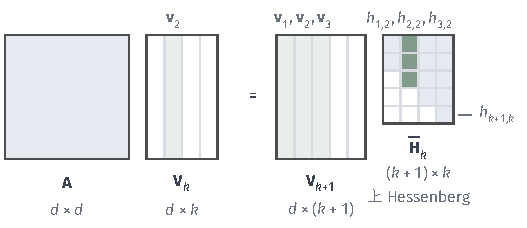
\includegraphics[width=89.098mm]{figures/01-basic-mathematics/03-vectors-matrices-and-multivariate-functions/tikz/c5-arnoldi-relation-shapes/figure.pdf}
  \caption{Arnoldi关系$\bm A\bm V_k=\bm V_{k+1}\overline{\bm H}_k$中各矩阵的形状（示意$d=7$、$k=4$）。$\overline{\bm H}_k$的非零元（浅蓝）只出现在主对角线、其上方和紧邻的下次对角线上，是上Hessenberg矩阵，末行只剩$h_{k+1,k}$。绿色标出第$j=2$列：$\bm A\bm v_2$只用到$\bm v_1,\bm v_2,\bm v_3$，系数是$\overline{\bm H}_k$第2列的前三个元素。}
  \label{fig:ls-arnoldi-relation-shapes}
\end{figure}

左乘$\bm V_k^\top$，并用$\bm V_k^\top\bm V_k=\bm I$与$\bm V_k^\top\bm v_{k+1}=\bm 0$，得
\begin{equation}
 \bm H_k=\bm V_k^\top\bm A\bm V_k .
 \label{eq:ls-arnoldi-projection}
\end{equation}
所以$\bm H_k$是$\bm A$在$\mathcal K_k$上的投影：若$\bm z=\bm V_k\bm y$是子空间中的向量，则$\bm A\bm z$在子空间中的分量的坐标为$\bm H_k\bm y$，伸出子空间的部分只沿$\bm v_{k+1}$一个方向，大小由$h_{k+1,k}$记录。

图中$\bm V_{k+1}$只比$\bm V_k$多一列，而$\overline{\bm H}_k$只有$k+1$行：$d$维矩阵在子空间上的作用，就这样被压缩成一个$k$阶的上Hessenberg矩阵。

\paragraph{正确性}
上面的论证用到了“此前各步的基已经标准正交”。下面的定理用归纳法确认这一点，并给出终止的情形。

\begin{theorem}[Arnoldi关系]
\label{thm:ls-arnoldi-relation}
在精确算术下按式~\eqref{eq:ls-arnoldi-coefficients}与\eqref{eq:ls-arnoldi-normalize}执行$k$轮Arnoldi正交化，且前$k-1$轮的$h_{j+1,j}$均非零。若$h_{k+1,k}\ne0$，则$\bm v_1,\ldots,\bm v_{k+1}$标准正交，$\bm v_1,\ldots,\bm v_j$张成$\mathcal K_j$（$j\le k+1$），关系~\eqref{eq:ls-arnoldi-relation}成立，并且$\bm H_k=\bm V_k^\top\bm A\bm V_k$。若$h_{k+1,k}=0$，则$\bm v_1,\ldots,\bm v_k$标准正交，$\bm A\bm V_k=\bm V_k\bm H_k$，$\mathcal K_k$在$\bm A$下不变；$\bm A$非奇异时精确解$\bm x_\star$属于$\bm x_0+\mathcal K_k$。
\end{theorem}

\begin{proof}
依次证明正交性、张成关系与矩阵关系，最后处理子空间不再扩张的情形。

\emph{正交性。}对$j$归纳，设$\bm v_1,\ldots,\bm v_j$标准正交。第$i$次扣除后$\bm w\perp\bm v_i$，此后扣除的方向$\bm v_{i+1},\ldots,\bm v_j$都与$\bm v_i$正交，不破坏这一关系，所以最终余项与$\bm v_1,\ldots,\bm v_j$都正交。$h_{j+1,j}\ne0$时归一化得到单位向量$\bm v_{j+1}$，与前$j$个正交。

\emph{张成与矩阵关系。}$\bm v_1\in\mathcal K_1$；若$\bm v_1,\ldots,\bm v_j\in\mathcal K_j$，则
\[
 \bm v_{j+1}\in\operatorname{span}\{\bm A\bm v_j,\bm v_1,\ldots,\bm v_j\}\subseteq\mathcal K_{j+1},
\]
$j+1$个标准正交向量落在维数不超过$j+1$的$\mathcal K_{j+1}$中，因而张成它。由式~\eqref{eq:ls-arnoldi-normalize}，扣除完毕后的余项就是$h_{j+1,j}\bm v_{j+1}$，把扣除的分量加回即得列关系~\eqref{eq:ls-arnoldi-column}，并排写出即是式~\eqref{eq:ls-arnoldi-relation}。左乘$\bm V_k^\top$，并用$\bm V_k^\top\bm V_k=\bm I$与$\bm V_k^\top\bm v_{k+1}=\bm 0$，得$\bm H_k=\bm V_k^\top\bm A\bm V_k$。

\emph{不再扩张的情形。}若$h_{k+1,k}=0$，第$k$列成为$\bm A\bm v_k=\sum_{i\le k}h_{i,k}\bm v_i$，于是$\bm A\bm V_k=\bm V_k\bm H_k$，$\bm A\mathcal K_k\subseteq\mathcal K_k$。$\bm A$非奇异时它在有限维空间$\mathcal K_k$上是单射，因而也是满射；$\bm r_0\in\mathcal K_k$，故有$\bm z\in\mathcal K_k$使$\bm A\bm z=\bm r_0$，$\bm x_\star=\bm x_0+\bm z$。
\end{proof}

$\mathcal K_k$的维数不超过$d$，所以至多$d$轮出现$h_{k+1,k}=0$。这时精确解已在候选集合中，使用这组基的求解器在这一步得到精确解，但仍须用原残差确认。

\paragraph{数值敏感度}
有限精度下基的正交性会逐渐损失，判断与补救办法沿用第~\ref{sec:ls-qr-method}节对修正Gram--Schmidt的讨论，必要时按“每轮的更新”所述再正交化。再正交化要用到全部已保存的基向量，Arnoldi正交化本来就保存它们，所以这一补救的代价只是多做一遍投影。

\paragraph{计算代价}
每轮一次$\bm A$乘向量。第$j$轮的扣除要作$j$次内积与$j$次向量更新，约$4dj$次浮点运算，$k$轮合计约$2dk^2$次；保存$\bm V_{k+1}$约需$(k+1)d$个数。两者都随轮数增长，原因是整组基都要保存并参与扣除。本过程只负责生成候选空间，收敛快慢由调用它的求解器在子空间中采用的选解准则决定。

\subsection{应用}
\label{sec:ls-arnoldi-application}

有了基与投影矩阵，就可以在子空间中求解方程。把近似写成
\[
 \bm x_k=\bm x_0+\bm V_k\bm y ,
\]
$\bm y\in\mathbb R^k$是子空间中的坐标。由$\bm r_0=\lVert\bm r_0\rVert_2\bm v_1=\bm V_{k+1}\lVert\bm r_0\rVert_2\bm e_1$与关系~\eqref{eq:ls-arnoldi-relation}，残差可以写成
\begin{equation}
 \bm r_0-\bm A\bm V_k\bm y=\bm V_{k+1}\bigl(\lVert\bm r_0\rVert_2\bm e_1-\overline{\bm H}_k\bm y\bigr),
 \label{eq:ls-arnoldi-residual-coordinates}
\end{equation}
其中$\bm e_1\in\mathbb R^{k+1}$。$d$维的残差由此用$k+1$个坐标表示出来。第~\ref{sec:ls-krylov-selection-criteria}节的准则都可以在这个小问题上实现。

按Galerkin条件，要求残差与$\mathcal K_k$正交，即$\bm V_k^\top(\bm r_0-\bm A\bm V_k\bm y)=\bm 0$。由$\bm H_k=\bm V_k^\top\bm A\bm V_k$，这就是$k$阶上Hessenberg方程组
\begin{equation}
 \bm H_k\bm y=\lVert\bm r_0\rVert_2\,\bm e_1 ,
 \label{eq:ls-arnoldi-galerkin-system}
\end{equation}
这里$\bm e_1\in\mathbb R^k$。

不过对非对称矩阵，Galerkin条件没有极小性，$\bm H_k$也可能奇异。按极小残差条件，则因$\bm V_{k+1}$的列标准正交、不改变长度，在子空间中求残差最小的坐标化为$(k+1)\times k$的小型最小二乘问题
\begin{equation}
 \min_{\bm y}\bigl\lVert\lVert\bm r_0\rVert_2\bm e_1-\overline{\bm H}_k\bm y\bigr\rVert_2 ,
 \label{eq:ls-arnoldi-minimal-residual-problem}
\end{equation}
它对任何非奇异的$\bm A$都有唯一解。这就是GMRES（第~\ref{sec:ls-gmres}节）的做法；$\overline{\bm H}_k$是上Hessenberg矩阵，每增加一列只需一次新的Givens旋转就能延续三角化。

这两种用法都要用$\bm V_k$还原$\bm x_k$，整组基须一直保存，存储与正交化工作随步数增长。实际计算因此常在做满$m$步后停下，以当前近似为新起点重新开始生成基，即\emph{重启}；它限制了存储，代价是失去跨周期的最优性。

\section{Lanczos正交化}
\label{sec:ls-lanczos}

第~\ref{sec:ls-arnoldi}节的Arnoldi正交化对一般方阵生成$\mathcal K_k(\bm A,\bm r_0)$的标准正交基，代价是每轮都要与全部旧基向量正交化。$\bm A$对称时，其中大部分系数自动为零。\term{Lanczos过程}（Lanczos process）就是Arnoldi正交化在对称矩阵上的简化：每轮只扣除两个方向，就生成同一组标准正交基，并把$\bm A$在子空间上的作用记录为一个对称三对角小矩阵。下面先推出三项递推，再写出计算过程，然后分析所得结果，最后说明它怎样用于求解方程；与Arnoldi正交化相同的论证只作引用。

\subsection{主要思想}

Lanczos过程的任务与Arnoldi正交化相同，只是矩阵对称：给定对称矩阵$\bm A\in\mathbb R^{d\times d}$、初始残差$\bm r_0\ne\bm 0$与步数$k$，生成标准正交向量$\bm v_1,\ldots,\bm v_k$，使前$j$个向量张成$\mathcal K_j(\bm A,\bm r_0)$，第一个向量取$\bm v_1=\bm r_0/\lVert\bm r_0\rVert_2$。

\paragraph{三项递推}
从第~\ref{sec:ls-arnoldi}节的系数出发。精确算术下，Arnoldi正交化在第$j$轮扣除的系数为
\[
 h_{i,j}=\bm v_i^\top\bm A\bm v_j\quad(i\le j),
\]
并且由列关系~\eqref{eq:ls-arnoldi-column}，每个$\bm A\bm v_i$都是$\bm v_1,\ldots,\bm v_{i+1}$的组合。$\bm A$对称时，
\[
 h_{i,j}=\bm v_i^\top\bm A\bm v_j=(\bm A\bm v_i)^\top\bm v_j .
\]
当$i+1<j$时，$\bm A\bm v_i$所含的$\bm v_1,\ldots,\bm v_{i+1}$都与$\bm v_j$正交，所以$h_{i,j}=0$；

当$i=j-1$时，$h_{j-1,j}=(\bm A\bm v_{j-1})^\top\bm v_j$恰是上一轮的归一化系数$h_{j,j-1}$。

于是第$j$轮只剩对角系数$h_{j,j}$与归一化系数$h_{j+1,j}$需要计算。记
\begin{equation}
 a_j=h_{j,j},\qquad \gamma_j=h_{j+1,j},
 \label{eq:ls-lanczos-coefficients}
\end{equation}
并约定$\bm v_0=\bm 0$、$\gamma_0=0$，列关系~\eqref{eq:ls-arnoldi-column}化为
\begin{equation}
 \bm A\bm v_j=\gamma_{j-1}\bm v_{j-1}+a_j\bm v_j+\gamma_j\bm v_{j+1},\qquad a_j=\bm v_j^\top\bm A\bm v_j ,
 \label{eq:ls-arnoldi-lanczos}
\end{equation}
这就是\term{Lanczos三项递推}（Lanczos recurrence）。计算新向量时只需用到紧邻的三个量$\bm A\bm v_j$、$\bm v_j$与$\bm v_{j-1}$，不必保存整组基。

图~\ref{fig:solver-lanczos-three-directions}把三项递推与三对角形状对应起来。固定第$j$列时，只需紧邻的三个基方向；其他位置的系数因对称性和正交性为零。

\begin{figure}[!htb]
  \centering
  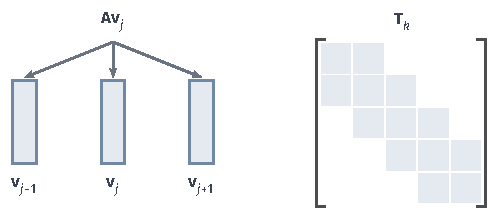
\includegraphics{figures/02-vectors-matrices-and-multivariate-calculus/03-linear-equations-and-optimization/tikz/learning-mechanisms/lanczos-three-directions.pdf}
  \caption{Lanczos过程在精确算术下的局部关系。左侧$\bm A\bm v_j$由$\bm v_{j-1},\bm v_j,\bm v_{j+1}$三个方向组成；右侧对称三对角矩阵$\bm T_k$只在主对角线和相邻两条对角线上可能非零。有限精度下可能需要重新正交化，图示不代表舍入后仍自动保持全局正交。}
  \label{fig:solver-lanczos-three-directions}
\end{figure}

\subsection{算法实现}

由三项递推~\eqref{eq:ls-arnoldi-lanczos}移项，每轮作一次矩阵乘向量，扣除两个方向，再把余项归一化。下面写出计算中用到的变量、它们怎样初始化、每轮怎样更新。下面用例~\ref{ex:ls-stationary-running-example}的以下数据逐步演示：
\[
 \bm A=\begin{bmatrix}4&1\\1&3\end{bmatrix},\qquad \bm b=\begin{bmatrix}1\\2\end{bmatrix}.
\]
取$\bm x_0=\bm 0$，于是$\bm r_0=\bm b$，步数取$k=2$。

\paragraph{变量}
\begin{itemize}
 \item $\bm v_{j-1},\bm v_j\in\mathbb R^d$：上一个与当前基向量，只保存这两个。
 \item $\bm w\in\mathbb R^d$：工作向量，先存$\bm A\bm v_j$，再在原处扣除两个方向，成为余项。
 \item $a_j$：第$j$个对角元。
 \item $\gamma_j$：第$j$个次对角元，也是$\bm v_{j+1}$的归一化系数；$\gamma_{j-1}$留到本轮扣除时使用。
 \item $j$：轮次。
\end{itemize}

\paragraph{初始化}
把上一个基向量初始化为零向量，$\gamma_0$初始化为零，第一个基向量初始化为初始残差的方向，轮次初始化为$1$：
\[
 \bm v_0=\bm 0,\qquad \gamma_0=0,\qquad \bm v_1=\frac{\bm r_0}{\lVert\bm r_0\rVert_2},\qquad j=1 .
\]
例中$\lVert\bm r_0\rVert_2=\sqrt5$，
\[
 \bm v_1=\frac1{\sqrt5}\begin{bmatrix}1\\2\end{bmatrix}.
\]

\paragraph{每轮更新}
在第$j$轮：
\begin{enumerate}
 \item \textbf{乘矩阵。}计算
 \[
  \bm w=\bm A\bm v_j .
 \]
 例中第一轮
 \[
   \bm w=\bm A\bm v_1=(6,7)^\top/\sqrt5 .
 \]

 \item \textbf{求对角元。}计算
 \[
  a_j=\bm v_j^\top\bm w .
 \]
 例中第一轮
 \[
   a_1=(1\cdot6+2\cdot7)/5=4 .
 \]

 \item \textbf{扣除两个方向。}计算
 \[
  \bm w\leftarrow\bm w-a_j\bm v_j-\gamma_{j-1}\bm v_{j-1} .
 \]
 例中第一轮$\gamma_0=0$，
 \[
  \bm w=\frac1{\sqrt5}\Bigl(\begin{bmatrix}6\\7\end{bmatrix}-4\begin{bmatrix}1\\2\end{bmatrix}\Bigr)=\frac1{\sqrt5}\begin{bmatrix}2\\-1\end{bmatrix}.
 \]

 \item \textbf{归一化。}计算
 \[
  \gamma_j=\lVert\bm w\rVert_2,\qquad \bm v_{j+1}=\frac{\bm w}{\gamma_j} .
 \]
 
 例中第一轮
 \[
  \gamma_1=1,\qquad \bm v_2=\frac1{\sqrt5}\begin{bmatrix}2\\-1\end{bmatrix}.
 \]
 然后令$j\leftarrow j+1$：$\bm v_j$成为下一轮的“上一个基向量”，$\bm v_{j+1}$成为“当前基向量”。

 例中第二轮先乘矩阵，得
 \[
  \bm w=\bm A\bm v_2=(7,-1)^\top/\sqrt5 ,
 \]
 再求对角元，
 \[
  a_2=\frac{14+1}{5}=3 .
 \]
 扣除$3\bm v_2$与$\gamma_1\bm v_1$后
 \[
  \bm w=\frac1{\sqrt5}\Bigl(\begin{bmatrix}7\\-1\end{bmatrix}-3\begin{bmatrix}2\\-1\end{bmatrix}-\begin{bmatrix}1\\2\end{bmatrix}\Bigr)=\bm 0 ,
 \]
 于是$\gamma_2=0$。

 \item \textbf{停止。}当$\gamma_j=0$（实际中低于按输入尺度取定的阈值）时，$\bm A\bm v_j$已落在现有空间中，Krylov子空间不再扩张，不作归一化，退出迭代；否则做满$k$轮后退出。例中第二轮$\gamma_2=0$，二维空间已经用尽，退出迭代。
\end{enumerate}
第1—4步合起来就是
\begin{equation}
 \begin{aligned}
 \bm w&=\bm A\bm v_j, & a_j&=\bm v_j^\top\bm w,\\
 \hat{\bm w}&=\bm w-a_j\bm v_j-\gamma_{j-1}\bm v_{j-1},\\
 \gamma_j&=\lVert\hat{\bm w}\rVert_2, & \bm v_{j+1}&=\hat{\bm w}/\gamma_j .
 \end{aligned}
 \label{eq:ls-lanczos-step}
\end{equation}
实际计算中也常先扣除$\gamma_{j-1}\bm v_{j-1}$，再用扣除后的向量求$a_j$：精确算术下结果相同，这与修正Gram--Schmidt的做法一致，有限精度下正交性略好。

最终得到标准正交基$\bm v_1,\bm v_2$与各轮系数组成的三对角矩阵。例中
\[
 \bm V_2=\frac1{\sqrt5}\begin{bmatrix}1&2\\2&-1\end{bmatrix},\qquad
 \bm T_2=\begin{bmatrix}a_1&\gamma_1\\\gamma_1&a_2\end{bmatrix}=\begin{bmatrix}4&1\\1&3\end{bmatrix},
\]
它们满足
\[
 \bm A\bm V_2=\bm V_2\bm T_2 .
\]
逐列核对：
\[
 \begin{gathered}
 4(1,2)^\top+(2,-1)^\top=(6,7)^\top,\\
 (1,2)^\top+3(2,-1)^\top=(7,-1)^\top ,
 \end{gathered}
\]
两边同除以$\sqrt5$即是$\bm A\bm v_1$与$\bm A\bm v_2$。

结果与第~\ref{sec:ls-arnoldi}节对同一矩阵算出的$\bm H_2$相同，但这里每轮只扣除了两个方向。

\subsection{算法分析}

\paragraph{基矩阵与投影矩阵}
与第~\ref{sec:ls-arnoldi}节一样，把各步的基并排成瘦长矩阵$\bm V_k=[\bm v_1,\ldots,\bm v_k]\in\mathbb R^{d\times k}$，它的列张成$\mathcal K_k$。把$j=1,\ldots,k$的递推式~\eqref{eq:ls-arnoldi-lanczos}按列并排写出，得到矩阵形式
\begin{equation}
 \bm A\bm V_k=\bm V_k\bm T_k+\gamma_k\bm v_{k+1}\bm e_k^\top=\bm V_{k+1}\overline{\bm T}_k ,
 \label{eq:ls-arnoldi-tridiagonal}
\end{equation}
其中
\begin{equation}
 \bm T_k=\begin{bmatrix}
 a_1&\gamma_1&&\\
 \gamma_1&a_2&\ddots&\\
 &\ddots&\ddots&\gamma_{k-1}\\
 &&\gamma_{k-1}&a_k
 \end{bmatrix},
 \label{eq:ls-lanczos-tridiagonal-matrix}
\end{equation}
$\overline{\bm T}_k$是在$\bm T_k$下方添一行$\gamma_k\bm e_k^\top$所得的$(k+1)\times k$矩阵。

左乘$\bm V_k^\top$，并用$\bm V_k^\top\bm V_k=\bm I$与$\bm V_k^\top\bm v_{k+1}=\bm 0$，得
\begin{equation}
 \bm T_k=\bm V_k^\top\bm A\bm V_k .
 \label{eq:ls-lanczos-projection}
\end{equation}
这正是Arnoldi关系~\eqref{eq:ls-arnoldi-relation}在对称情形下的形式：
\[
  \overline{\bm H}_k=\overline{\bm T}_k,\qquad \bm H_k=\bm T_k .
\]

$\bm T_k$同样是$\bm A$在$\mathcal K_k$上的投影，即子空间中向量的像在子空间中的坐标由$\bm T_k$给出；不同的是，它不仅是上Hessenberg矩阵，而且对称，因而是三对角的。

$d$维对称矩阵在子空间上的作用，就这样被压缩成一个$k$阶对称三对角矩阵，只需$2k-1$个数$a_1,\ldots,a_k$与$\gamma_1,\ldots,\gamma_{k-1}$记录。

\paragraph{正确性}
推导三项递推时用到了“此前各步的基已经标准正交”，这是由完整扣除保证的；只扣除两项时需要重新确认。下面的定理用归纳法证明这一点，并给出终止的情形。

\begin{theorem}[Lanczos关系]
\label{thm:ls-arnoldi-lanczos}
设$\bm A$对称，$\bm r_0\ne\bm 0$，在精确算术下按式~\eqref{eq:ls-lanczos-step}执行$k$轮，且$\gamma_1,\ldots,\gamma_{k-1}$均非零。若$\gamma_k\ne0$，则$\bm v_1,\ldots,\bm v_{k+1}$标准正交，$\bm v_1,\ldots,\bm v_j$张成$\mathcal K_j$（$j\le k+1$），关系~\eqref{eq:ls-arnoldi-tridiagonal}成立，并且$\bm T_k=\bm V_k^\top\bm A\bm V_k$。若$\gamma_k=0$，则$\bm v_1,\ldots,\bm v_k$标准正交，$\bm A\bm V_k=\bm V_k\bm T_k$，$\mathcal K_k$在$\bm A$下不变；$\bm A$非奇异时精确解$\bm x_\star$属于$\bm x_0+\mathcal K_k$。
\end{theorem}

\begin{proof}
依次证明正交性、张成关系与矩阵关系，最后处理子空间不再扩张的情形。

\emph{正交性。}对$j$归纳，设$\bm v_1,\ldots,\bm v_j$标准正交，且对$i<j$式~\eqref{eq:ls-arnoldi-lanczos}成立。只需证明扣除后的$\hat{\bm w}=\bm A\bm v_j-a_j\bm v_j-\gamma_{j-1}\bm v_{j-1}$与$\bm v_1,\ldots,\bm v_j$都正交。对$i=j$，由$a_j=\bm v_j^\top\bm A\bm v_j$，$\bm v_j^\top\hat{\bm w}=0$。对$i<j$，由对称性$\bm v_i^\top\bm A\bm v_j=(\bm A\bm v_i)^\top\bm v_j$，而$\bm A\bm v_i=\gamma_{i-1}\bm v_{i-1}+a_i\bm v_i+\gamma_i\bm v_{i+1}$，所以
\[
 \bm v_i^\top\bm A\bm v_j=\gamma_i\,\bm v_{i+1}^\top\bm v_j=
 \begin{cases}\gamma_{j-1},&i=j-1,\\0,&i<j-1.\end{cases}
\]
再由$\bm v_i^\top\bm v_{j-1}$与$\bm v_i^\top\bm v_j$的取值，$i=j-1$时$\bm v_{j-1}^\top\hat{\bm w}=\gamma_{j-1}-\gamma_{j-1}=0$，$i<j-1$时三项都为零。$\gamma_j\ne0$时归一化得到单位向量$\bm v_{j+1}$，与前$j$个正交。

\emph{张成与矩阵关系。}$\bm v_1\in\mathcal K_1$；若$\bm v_{j-1},\bm v_j\in\mathcal K_j$，则
\[
 \bm v_{j+1}\in\operatorname{span}\{\bm A\bm v_j,\bm v_j,\bm v_{j-1}\}\subseteq\mathcal K_{j+1},
\]
$j+1$个标准正交向量落在维数不超过$j+1$的$\mathcal K_{j+1}$中，因而张成它。由式~\eqref{eq:ls-lanczos-step}，$\gamma_j\bm v_{j+1}$就是扣除后的余项，把扣除的两项加回即得列关系~\eqref{eq:ls-arnoldi-lanczos}，并排写出即是式~\eqref{eq:ls-arnoldi-tridiagonal}。左乘$\bm V_k^\top$，并用$\bm V_k^\top\bm V_k=\bm I$与$\bm V_k^\top\bm v_{k+1}=\bm 0$，得$\bm T_k=\bm V_k^\top\bm A\bm V_k$。

\emph{不再扩张的情形。}若$\gamma_k=0$，第$k$列成为$\bm A\bm v_k=\gamma_{k-1}\bm v_{k-1}+a_k\bm v_k$，于是$\bm A\bm V_k=\bm V_k\bm T_k$，$\bm A\mathcal K_k\subseteq\mathcal K_k$。$\bm A$非奇异时它在有限维空间$\mathcal K_k$上是单射，因而也是满射；$\bm r_0\in\mathcal K_k$，故有$\bm z\in\mathcal K_k$使$\bm A\bm z=\bm r_0$，$\bm x_\star=\bm x_0+\bm z$。
\end{proof}

定理表明，精确算术下只扣除两项与扣除全部已有分量结果相同：被省略的系数$\bm v_i^\top\bm A\bm v_j$（$i<j-1$）本来就是零。第~\ref{sec:ls-arnoldi}节对一般方阵扣除全部已有分量，得到上Hessenberg小矩阵；$\bm A$对称时它退化为这里的$\bm T_k$，两种过程给出相同的基与系数，贯穿例上两节的数值也完全一致。$\mathcal K_k$的维数不超过$d$，所以至多$d$轮出现$\gamma_k=0$。

\paragraph{数值敏感度}
有限精度下，正交性依赖的相消只近似成立。三项递推只对最近两个方向扣除，舍入引入的旧方向分量不会被去掉，并且会随迭代放大，基的正交性损失比第~\ref{sec:ls-arnoldi}节的完整正交化明显；典型的表现是$\bm T_k$的特征值中出现$\bm A$同一特征值的多个近似副本。保存全部基并再正交化可以补救，但这就失去了固定存储的优点；不保存基时，调用它的求解器只能靠真实残差复核控制结果。

\paragraph{计算代价}
每轮一次$\bm A$乘向量，此外只有两次内积（其一用于求$\gamma_j$）、两次向量更新和一次缩放，约$9d$次浮点运算；除矩阵外保存$\bm v_{j-1},\bm v_j,\bm w$三个向量，存储不随轮数增长。与Arnoldi正交化$k$轮约$2dk^2$次运算、$(k+1)d$个数的存储相比，这是利用对称性得到的主要收益。本过程只负责生成候选空间，收敛快慢由调用它的求解器在子空间中采用的选解准则决定。

\subsection{应用}
\label{sec:ls-lanczos-application}

用法与第~\ref{sec:ls-arnoldi-application}节相同：把近似写成$\bm x_k=\bm x_0+\bm V_k\bm y$，$\bm y\in\mathbb R^k$是子空间中的坐标，再按某个准则确定$\bm y$。

按Galerkin条件，$\bm V_k^\top(\bm r_0-\bm A\bm V_k\bm y)=\bm0$，由$\bm r_0=\lVert\bm r_0\rVert_2\bm v_1$与$\bm T_k=\bm V_k^\top\bm A\bm V_k$，得到$k$阶三对角方程组
\begin{equation}
 \bm T_k\bm y=\lVert\bm r_0\rVert_2\,\bm e_1 .
 \label{eq:ls-lanczos-projected-system}
\end{equation}
它只有$k\times k$大小，又是三对角的，用第~\ref{sec:ls-lu}节的消元约$O(k)$次运算即可解出；解出坐标$\bm y$后，再用$\bm V_k$还原，就得到原空间中的近似解$\bm x_k$。

这就是后面两种对称矩阵求解器的共同骨架。对称正定时，$\bm T_k$也对称正定，方程~\eqref{eq:ls-lanczos-projected-system}总有唯一解，所得近似就是CG的迭代值（第~\ref{sec:ls-conjugate-gradient}节）；CG还利用$\bm T_k$的分解随步数延伸的结构，把求解与还原合并为短递推，连基$\bm V_k$也不必保存。

对称不定时，$\bm T_k$可能奇异，MINRES（第~\ref{sec:ls-minres}节）改用$(k+1)\times k$的$\overline{\bm T}_k$，在子空间中求残差最小的坐标：
\begin{equation}
 \min_{\bm y}\bigl\lVert\lVert\bm r_0\rVert_2\bm e_1-\overline{\bm T}_k\bm y\bigr\rVert_2 .
 \label{eq:ls-lanczos-minimal-residual-problem}
\end{equation}

两者的子空间、基和三对角矩阵都来自同一个Lanczos过程，区别只在于用哪一种准则确定坐标$\bm y$。

\section{Golub--Kahan双对角化}
\label{sec:ls-bidiagonal-iteration}

第~\ref{sec:ls-arnoldi}节的Arnoldi正交化与第~\ref{sec:ls-lanczos}节的Lanczos过程都针对方阵：残差与未知量同在$d$维空间，可以把残差反复乘$\bm A$。长方或秩亏的最小二乘问题中，$\bm A\in\mathbb R^{m\times d}$的残差在$m$维的数据空间，未知量在$d$维空间，不能把残差反复乘$\bm A$；把数据空间的向量送回未知量空间的是$\bm A^\top$。

这时需要的是第~\ref{sec:ls-krylov-subspaces}节所说的Krylov空间$\mathcal K_k(\bm A^\top\bm A,\bm A^\top\bm b)$。$\bm A^\top\bm A$对称半正定，原则上可以对它作Lanczos过程，但形成$\bm A^\top\bm A$会损失信息。\term{Golub--Kahan双对角化}（Golub--Kahan bidiagonalization）交替作用$\bm A$与$\bm A^\top$，只用$\bm A\bm v$与$\bm A^\top\bm u$，就得到与对$\bm A^\top\bm A$作Lanczos过程相同的基，并把$\bm A$压缩成一个双对角小矩阵。下面先推出两项递推，再写出计算过程，然后分析所得结果，最后说明它怎样用于求解最小二乘问题。

\subsection{主要思想}

给定$\bm A\in\mathbb R^{m\times d}$（可以秩亏）、$\bm b\in\mathbb R^m$与步数$k$，取零初值，初始残差就是$\bm b$。双对角化要在数据空间生成标准正交基$\bm u_1,\ldots,\bm u_{k+1}$，在未知量空间生成与之配对的标准正交基$\bm v_1,\ldots,\bm v_k$，使前$j$个$\bm v$张成$\mathcal K_j(\bm A^\top\bm A,\bm A^\top\bm b)$。第一对向量取$\bm u_1=\bm b/\lVert\bm b\rVert_2$，$\bm v_1$取$\bm A^\top\bm u_1$的方向。两组向量属于不同的空间，各自在本空间内正交。

\paragraph{交替的两项递推}
仿照第~\ref{sec:ls-arnoldi}节，新向量都由“乘矩阵、扣除旧基向量的分量、归一化”得到，只是$\bm A$与$\bm A^\top$交替使用：$\bm u_{j+1}$由$\bm A\bm v_j$对$\bm u_1,\ldots,\bm u_j$正交化得到，$\bm v_{j+1}$由$\bm A^\top\bm u_{j+1}$对$\bm v_1,\ldots,\bm v_j$正交化得到。

设此前的基已分别标准正交。按构造，每个$\bm A^\top\bm u_i$都是$\bm v_1,\ldots,\bm v_i$的组合，每个$\bm A\bm v_i$都是$\bm u_1,\ldots,\bm u_{i+1}$的组合。

于是$\bm A\bm v_j$在$\bm u_i$上的系数为
\[
 \bm u_i^\top\bm A\bm v_j=(\bm A^\top\bm u_i)^\top\bm v_j ,
\]
当$i<j$时$\bm A^\top\bm u_i$所含的$\bm v_1,\ldots,\bm v_i$都与$\bm v_j$正交，系数为零，只剩$i=j$一项。

同样，$\bm A^\top\bm u_{j+1}$在$\bm v_i$上的系数为
\[
 \bm v_i^\top\bm A^\top\bm u_{j+1}=(\bm A\bm v_i)^\top\bm u_{j+1} ,
\]
当$i<j$时$\bm A\bm v_i$所含的$\bm u_1,\ldots,\bm u_{i+1}$都与$\bm u_{j+1}$正交，系数为零，只剩$i=j$一项。

所以每生成一个新向量只需扣除对面空间中相邻的一个方向。把扣除的系数与归一化系数记为$\alpha_i,\beta_i\ge0$，并约定$\bm v_0=\bm 0$，列关系为
\begin{equation}
 \bm A\bm v_i=\alpha_i\bm u_i+\beta_{i+1}\bm u_{i+1},\qquad
 \bm A^\top\bm u_i=\beta_i\bm v_{i-1}+\alpha_i\bm v_i .
 \label{eq:ls-golub-kahan-columns}
\end{equation}

由第二式，$\bm A\bm v_j$在$\bm u_j$上的系数$(\bm A^\top\bm u_j)^\top\bm v_j$正是$\alpha_j$；由第一式，$\bm A^\top\bm u_{j+1}$在$\bm v_j$上的系数$(\bm A\bm v_j)^\top\bm u_{j+1}$正是$\beta_{j+1}$。因此扣除用的系数就是上一步的归一化系数，不必另作内积。

与Arnoldi正交化的列关系~\eqref{eq:ls-arnoldi-column}相比，每个像只用到对面空间中的两个基向量，不必保存整组基；这与Lanczos过程只需三项的原因相同，算法分析中将看到，右侧基正是$\bm A^\top\bm A$的Lanczos基。

\subsection{计算过程}

由列关系~\eqref{eq:ls-golub-kahan-columns}移项，每轮先作一次$\bm A$乘向量、扣除一个方向并归一化，得到新的$\bm u$，再作一次$\bm A^\top$乘向量、扣除一个方向并归一化，得到新的$\bm v$。下面写出计算中用到的变量、它们怎样初始化、每轮怎样更新。下面用以下不相容的长方系统逐步演示：
\[
 \bm A=\begin{bmatrix}1&0\\0&2\\0&0\end{bmatrix},\qquad
 \bm b=\begin{bmatrix}1\\1\\1\end{bmatrix}.
\]
第三行恒为零，$\bm b$的第三个分量无法拟合；最小二乘解是$\hat{\bm x}=(1,1/2)^\top$，最优残差为$(0,0,1)^\top$。这个例子的系数都有封闭形式，第~\ref{sec:ls-lsqr}节的LSQR与第~\ref{sec:ls-lsmr}节的LSMR继续用它，以便对照。

\paragraph{变量}
\begin{itemize}
 \item $\bm u_j\in\mathbb R^m$、$\bm v_j\in\mathbb R^d$：当前的两个基向量，只保存这两个；是否保存整组基由调用者决定。
 \item $\bm p\in\mathbb R^m$、$\bm q\in\mathbb R^d$：工作向量，分别存放数据空间与未知量空间中扣除后的余项。
 \item $\alpha_j$：$\bm B_k$的第$j$个对角元，也是$\bm v_j$的归一化系数。
 \item $\beta_j$：$\bm B_k$的第$j-1$列的次对角元（$\beta_1$为$\lVert\bm b\rVert_2$），也是$\bm u_j$的归一化系数。
 \item $j$：轮次。
\end{itemize}

\paragraph{初始化}
把$\bm u_1$初始化为$\bm b$的方向，再由列关系~\eqref{eq:ls-golub-kahan-columns}第二式在$i=1$时的$\bm A^\top\bm u_1=\alpha_1\bm v_1$把$\bm v_1$初始化为$\bm A^\top\bm u_1$的方向，轮次初始化为$1$：
\begin{equation}
 \begin{gathered}
 \beta_1=\lVert\bm b\rVert_2,\qquad \bm u_1=\frac{\bm b}{\beta_1},\\
 \alpha_1=\lVert\bm A^\top\bm u_1\rVert_2,\qquad \bm v_1=\frac{\bm A^\top\bm u_1}{\alpha_1}.
 \end{gathered}
 \label{eq:ls-golub-kahan-start}
\end{equation}
于是$\bm b=\beta_1\bm u_1$，而$\bm v_1$与$\bm A^\top\bm b$同向。

若$\bm b=\bm 0$，零向量满足方程；若$\alpha_1=0$，则$\bm A^\top\bm b=\bm 0$，零向量已满足正规方程~\eqref{eq:linear-algebra-normal-equations}。这两种情形都由求解器直接输出零向量，不再迭代。

例中$\beta_1=\sqrt3$，
\[
 \bm u_1=\frac1{\sqrt3}\begin{bmatrix}1\\1\\1\end{bmatrix},\qquad
 \bm A^\top\bm u_1=\frac1{\sqrt3}\begin{bmatrix}1\\2\end{bmatrix},
\]
故
\[
 \alpha_1=\sqrt{\frac53},\qquad \bm v_1=\frac{1}{\sqrt5}\begin{bmatrix}1\\2\end{bmatrix}.
\]

\paragraph{每轮更新}
在第$j$轮：
\begin{enumerate}
 \item \textbf{送到数据空间并扣除。}由列关系第一式（取$i=j$）移项，计算
 \[
  \bm p=\bm A\bm v_j-\alpha_j\bm u_j .
 \]
 例中第一轮
 \[
  \bm A\bm v_1=(1,4,0)^\top/\sqrt5,\qquad \alpha_1\bm u_1=\sqrt5(1,1,1)^\top/3 ,
 \]
 相减得
 \[
  \bm p=\frac{1}{3\sqrt5}\begin{bmatrix}-2\\7\\-5\end{bmatrix}.
 \]

 \item \textbf{归一化得到$\bm u_{j+1}$。}计算
 \[
  \beta_{j+1}=\lVert\bm p\rVert_2,\qquad \bm u_{j+1}=\frac{\bm p}{\beta_{j+1}} .
 \]
 例中第一轮
 \[
  \beta_2=\frac{\sqrt{78}}{3\sqrt5}\approx1.3166,\qquad
  \bm u_2=\frac{1}{\sqrt{78}}\begin{bmatrix}-2\\7\\-5\end{bmatrix}.
 \]

 \item \textbf{送回未知量空间并扣除。}由列关系第二式（取$i=j+1$）移项，计算
 \[
  \bm q=\bm A^\top\bm u_{j+1}-\beta_{j+1}\bm v_j .
 \]
 例中第一轮
 \[
  \bm A^\top\bm u_2=(-2,14)^\top/\sqrt{78},\qquad \beta_2\bm v_1=\sqrt{78}(1,2)^\top/15 ,
 \]
 相减得
 \[
  \bm q=\frac{18}{5\sqrt{78}}\begin{bmatrix}-2\\1\end{bmatrix}.
 \]

 \item \textbf{归一化得到$\bm v_{j+1}$。}计算
 \[
  \alpha_{j+1}=\lVert\bm q\rVert_2,\qquad \bm v_{j+1}=\frac{\bm q}{\alpha_{j+1}} .
 \]
 例中第一轮
 \[
  \alpha_2=\frac{18\sqrt5}{5\sqrt{78}}\approx0.9115,\qquad
  \bm v_2=\frac{1}{\sqrt5}\begin{bmatrix}-2\\1\end{bmatrix}.
 \]
 然后把本轮的$\beta_{j+1},\alpha_{j+1}$及新基向量交给调用它的求解器，令$j\leftarrow j+1$。

 例中第二轮
 \[
  \bm p=\bm A\bm v_2-\alpha_2\bm u_2=\frac{5}{13\sqrt5}\begin{bmatrix}-4\\1\\3\end{bmatrix},
 \]
 归一化得
 \[
  \beta_3=\sqrt{\frac{10}{13}}\approx0.8771,\qquad
  \bm u_3=\frac1{\sqrt{26}}\begin{bmatrix}-4\\1\\3\end{bmatrix};
 \]
 再送回未知量空间，
 \[
  \bm A^\top\bm u_3=(-4,2)^\top/\sqrt{26}
 \]
 恰好等于$\beta_3\bm v_2$，所以
 \[
  \bm q=\bm 0,\qquad \alpha_3=0 .
 \]

 \item \textbf{停止。}若$\beta_{j+1}=0$（实际中低于按数据尺度取定的阈值），则$\bm A\bm v_j=\alpha_j\bm u_j$，不生成$\bm u_{j+1}$，约定$\alpha_{j+1}=0$并退出迭代；若$\beta_{j+1}>0$而$\alpha_{j+1}=0$，则$\bm A^\top\bm u_{j+1}=\beta_{j+1}\bm v_j$已由现有的基表示，不生成$\bm v_{j+1}$，退出迭代；否则在求解器决定继续时进入下一轮，至多做满$k$轮。
 
 两种情况下略去未生成的基向量及其零系数，列关系~\eqref{eq:ls-golub-kahan-columns}仍成立；求解器照常用本轮的系数完成解的更新后再结束。基停止扩张不等于原残差为零：不相容问题的原残差可以停在非零值上。
 
 例中第二轮$\alpha_3=0$，未知量空间只有二维，已被$\bm v_1,\bm v_2$取尽，退出迭代。
\end{enumerate}
第1—4步合起来就是
\begin{equation}
 \begin{aligned}
 \bm p&=\bm A\bm v_j-\alpha_j\bm u_j, & \beta_{j+1}&=\lVert\bm p\rVert_2, & \bm u_{j+1}&=\bm p/\beta_{j+1},\\
 \bm q&=\bm A^\top\bm u_{j+1}-\beta_{j+1}\bm v_j, & \alpha_{j+1}&=\lVert\bm q\rVert_2, & \bm v_{j+1}&=\bm q/\alpha_{j+1} .
 \end{aligned}
 \label{eq:ls-golub-kahan-step}
\end{equation}

最终得到两组标准正交基与各轮系数组成的下双对角矩阵。例中$\bm U_3=[\bm u_1\;\bm u_2\;\bm u_3]$，
\[
 \bm V_2=\frac1{\sqrt5}\begin{bmatrix}1&-2\\2&1\end{bmatrix},\qquad
 \bm B_2=\begin{bmatrix}\alpha_1&0\\\beta_2&\alpha_2\\0&\beta_3\end{bmatrix}
 \approx\begin{bmatrix}1.2910&0\\1.3166&0.9115\\0&0.8771\end{bmatrix},
\]
它们满足
\[
 \bm A\bm V_2=\bm U_3\bm B_2 .
\]
逐列核对：
\[
 \begin{gathered}
 \alpha_1\bm u_1+\beta_2\bm u_2=(1,4,0)^\top/\sqrt5=\bm A\bm v_1,\\
 \alpha_2\bm u_2+\beta_3\bm u_3=(-2,2,0)^\top/\sqrt5=\bm A\bm v_2 .
 \end{gathered}
\]
右侧二维空间已经生成完毕，但$\bm b$的第三个分量仍不可拟合，原残差不会降到零。

上面的例子中基向量都有简单的封闭形式。对稠密的矩阵，可以只用双对角系数本身来核对计算，下面在直线拟合上演示。

\begin{example}[直线拟合上的两步双对角化]
\label{ex:ls-golub-kahan-line}
沿用示例~\ref{ex:ls-line-least-squares}的数据：
\[
 \bm A=\begin{bmatrix}1&0\\1&1\\1&2\end{bmatrix},\qquad
 \bm b=\begin{bmatrix}1\\2\\2\end{bmatrix}.
\]
起步得
\[
 \beta_1=3,\qquad \bm u_1=(1,2,2)^\top/3 ;
\]
再由$\bm A^\top\bm u_1=(5/3,2)^\top$得
\[
 \alpha_1=\sqrt{61}/3\approx2.6034,\qquad \bm v_1=(5,6)^\top/\sqrt{61} .
\]

第一轮先把$\bm v_1$送到数据空间并扣除$\alpha_1\bm u_1$：
\[
 \begin{gathered}
 \bm A\bm v_1=\frac{(5,11,17)^\top}{\sqrt{61}},\\
 \bm p=\bm A\bm v_1-\alpha_1\bm u_1=\frac{(-16,-23,31)^\top}{9\sqrt{61}},
 \end{gathered}
\]
于是
\[
  \beta_2\approx0.5944, \qquad \bm u_2\approx(-0.3829,-0.5504,0.7419)^\top .
\]
再由$\bm A^\top\bm u_2-\beta_2\bm v_1$得
\[
  \alpha_2\approx0.7446, \qquad \bm v_2=(-6,5)^\top/\sqrt{61} .
\]

第二轮得
\[
  \beta_3\approx0.5607, \qquad \bm u_3\approx(-0.8615,0.5026,-0.0718)^\top ,
\]
而$\bm A^\top\bm u_3-\beta_3\bm v_2=\bm0$，即$\alpha_3=0$：未知量空间只有二维，已被$\bm v_1,\bm v_2$取尽，生成到此为止。

最后核对结果。$\bm u_1,\bm u_2,\bm u_3$两两正交；$\bm V_2$是正交方阵，$\bm A=\bm U_3\bm B_2\bm V_2^\top$，所以$\bm B_2^\top\bm B_2$与$\bm A^\top\bm A=\left[\begin{smallmatrix}3&3\\3&5\end{smallmatrix}\right]$有相同的迹$8$和行列式$6$。数值上
\[
 \begin{gathered}
 \alpha_1^2+\beta_2^2+\alpha_2^2+\beta_3^2\approx8.000,\\
 \alpha_1^2\alpha_2^2+\alpha_1^2\beta_3^2+\beta_2^2\beta_3^2\approx6.000 .
 \end{gathered}
\]
两个不变量都吻合。这项核对只用到双对角系数本身，不必重新比较各个基向量。
\end{example}

\subsection{算法分析}

\paragraph{基矩阵与投影矩阵}
把各步得到的两组基分别并排，记
\begin{equation}
 \bm U_{k+1}=[\bm u_1\;\cdots\;\bm u_{k+1}]\in\mathbb R^{m\times(k+1)},\qquad
 \bm V_k=[\bm v_1\;\cdots\;\bm v_k]\in\mathbb R^{d\times k},
 \label{eq:ls-golub-kahan-bases}
\end{equation}
两者通常都是瘦长矩阵。

把$i=1,\ldots,k$的第一式与$i=1,\ldots,k+1$的第二式分别并排写出，得到
\begin{equation}
 \bm A\bm V_k=\bm U_{k+1}\bm B_k,\qquad
 \bm A^\top\bm U_{k+1}=\bm V_k\bm B_k^\top+\alpha_{k+1}\bm v_{k+1}\bm e_{k+1}^\top ,
 \label{eq:ls-golub-kahan-relations}
\end{equation}
其中
\begin{equation}
 \bm B_k=
 \begin{bmatrix}
 \alpha_1&&&\\
 \beta_2&\alpha_2&&\\
 &\beta_3&\ddots&\\
 &&\ddots&\alpha_k\\
 &&&\beta_{k+1}
 \end{bmatrix}
 \label{eq:ls-golub-kahan-bidiagonal-matrix}
\end{equation}
是$(k+1)\times k$的下双对角矩阵，第$i$列只有$\alpha_i$和它下方的$\beta_{i+1}$。后一式的边界项来自$\bm u_{k+1}$被$\bm A^\top$送回时产生的新方向；$\alpha_{k+1}=0$时它为零。

第一式左乘$\bm U_{k+1}^\top$，并用$\bm U_{k+1}^\top\bm U_{k+1}=\bm I$，得
\begin{equation}
 \bm B_k=\bm U_{k+1}^\top\bm A\bm V_k .
 \label{eq:ls-golub-kahan-projection}
\end{equation}
所以$\bm B_k$是$\bm A$从$\operatorname{range}(\bm V_k)$到$\operatorname{range}(\bm U_{k+1})$的坐标矩阵：若$\bm z=\bm V_k\bm y$，则$\bm A\bm z=\bm U_{k+1}\bm B_k\bm y$完全落在$\operatorname{range}(\bm U_{k+1})$中，坐标为$\bm B_k\bm y$。$m\times d$的长方矩阵就这样被压缩成一个$(k+1)\times k$的下双对角矩阵，只需$2k$个数记录。

再由第一式，
\begin{equation}
 \bm V_k^\top\bm A^\top\bm A\bm V_k=\bm B_k^\top\bm U_{k+1}^\top\bm U_{k+1}\bm B_k=\bm B_k^\top\bm B_k ,
 \label{eq:ls-golub-kahan-normal-projection}
\end{equation}
$\bm B_k^\top\bm B_k$是对称三对角矩阵，对角元为$\alpha_i^2+\beta_{i+1}^2$，次对角元为$\alpha_{i+1}\beta_{i+1}$；它就是对称半正定矩阵$\bm A^\top\bm A$在$\operatorname{range}(\bm V_k)$上的投影，相当于对$\bm A^\top\bm A$作Lanczos过程得到的$\bm T_k$。

\paragraph{正确性}
上面的论证用到了两组基的标准正交性，而每步只扣除一项。下面的定理说明，短递推~\eqref{eq:ls-golub-kahan-step}得到的两组基确实标准正交，关系~\eqref{eq:ls-golub-kahan-relations}成立，并且右侧基张成正规方程的Krylov空间。

\begin{theorem}[Golub--Kahan关系]
\label{thm:ls-golub-kahan-relations}
设$\alpha_1,\ldots,\alpha_k$与$\beta_2,\ldots,\beta_{k+1}$都为正。则在精确算术中，$\bm U_{k+1}$与$\bm V_k$的列分别标准正交，关系~\eqref{eq:ls-golub-kahan-relations}成立，其中$\alpha_{k+1}=0$时末项为零；并且$\operatorname{range}(\bm V_k)=\mathcal K_k(\bm A^\top\bm A,\bm A^\top\bm b)$。
\end{theorem}

\begin{proof}
先说明矩阵关系只是列关系的汇总，再对轮数归纳证明正交性，最后确定右侧基张成的空间。

\emph{列关系。}由式~\eqref{eq:ls-golub-kahan-start}与\eqref{eq:ls-golub-kahan-step}中$\bm p,\bm q$的定义，列关系~\eqref{eq:ls-golub-kahan-columns}成立。$\bm B_k^\top$的第$i$列是$\bm B_k$的第$i$行，所以它们分别是式~\eqref{eq:ls-golub-kahan-relations}两式的第$i$列；第二式第$k+1$列中$\alpha_{k+1}\bm v_{k+1}$一项不在$\bm V_k$中，单独写成边界项。

\emph{正交性。}设$\bm u_1,\ldots,\bm u_k$与$\bm v_1,\ldots,\bm v_k$已分别标准正交。对$j\le k$，由列关系，
\[
 \begin{aligned}
 \beta_{k+1}\bm u_j^\top\bm u_{k+1}
 &=\bm v_k^\top\bm A^\top\bm u_j-\alpha_k\bm u_j^\top\bm u_k\\
 &=\bm v_k^\top(\beta_j\bm v_{j-1}+\alpha_j\bm v_j)-\alpha_k\delta_{j,k}=0 .
 \end{aligned}
\]
再由$\bm A\bm v_j=\alpha_j\bm u_j+\beta_{j+1}\bm u_{j+1}$以及刚证明的$\bm u$的正交性，
\[
 \alpha_{k+1}\bm v_j^\top\bm v_{k+1}=\bm u_{k+1}^\top\bm A\bm v_j-\beta_{k+1}\delta_{j,k}=\beta_{j+1}\delta_{j,k}-\beta_{k+1}\delta_{j,k}=0 .
\]

\emph{张成的空间。}$\bm v_1\parallel\bm A^\top\bm b$；把两条列关系代入$\bm A^\top\bm A\bm v_i$，得
\[
 \alpha_{i+1}\beta_{i+1}\bm v_{i+1}=\bm A^\top\bm A\bm v_i-(\alpha_i^2+\beta_{i+1}^2)\bm v_i-\alpha_i\beta_i\bm v_{i-1},
\]
归纳可知$\bm v_i\in\mathcal K_i(\bm A^\top\bm A,\bm A^\top\bm b)$。$\bm V_k$的$k$列标准正交，而该Krylov空间至多$k$维，两者相等。
\end{proof}

因此零初值下双对角化生成的正是第~\ref{sec:ls-krylov-subspaces}节所说的长方矩阵Krylov空间，但从不形成$\bm A^\top\bm A$。证明中的三项关系就是对$\bm A^\top\bm A$从$\bm A^\top\bm b$出发的Lanczos递推~\eqref{eq:ls-arnoldi-lanczos}，其中$a_i=\alpha_i^2+\beta_{i+1}^2$、$\gamma_i=\alpha_{i+1}\beta_{i+1}$，正是$\bm B_k^\top\bm B_k$的元素。图~\ref{fig:ls-golub-kahan-bidiagonal}把递推与矩阵关系放在一起：(a)中进出$\bm v_i$的两支箭头给出$\alpha_i$与$\beta_{i+1}$，它们正是(b)中$\bm B_k$的第$i$列；每个新向量只与对面空间中相邻的一个向量相连，这就是每步只需扣除一项的原因。

\begin{figure}[htbp]
  \centering
  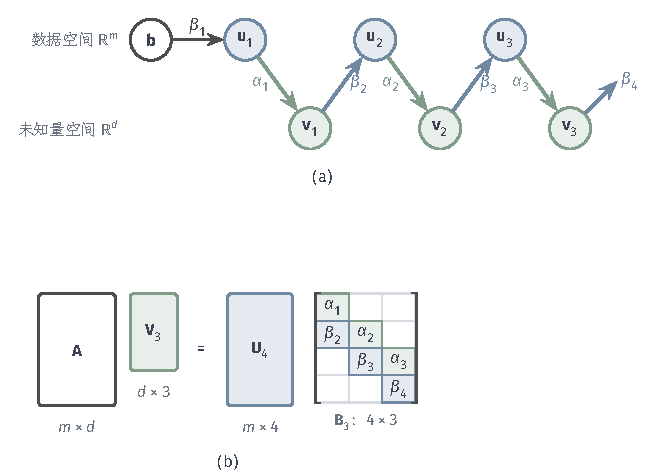
\includegraphics[width=109.343mm]{figures/01-basic-mathematics/03-vectors-matrices-and-multivariate-functions/tikz/c5-golub-kahan-bidiagonal/figure.pdf}
  \caption{Golub--Kahan双对角化的递推与矩阵关系（$k=3$）。(a)蓝色$\bm u_i$在数据空间，绿色$\bm v_i$在未知量空间；乘$\bm A^\top$并扣除前一个$\bm v$后归一化得到$\bm v_i$，长度为$\alpha_i$，乘$\bm A$并扣除前一个$\bm u$后归一化得到$\bm u_{i+1}$，长度为$\beta_{i+1}$。(b)这些长度排成$4\times3$的下双对角矩阵$\bm B_3$，满足$\bm A\bm V_3=\bm U_4\bm B_3$；绿格为对角元，蓝格为次对角元，其余元素为零。}
  \label{fig:ls-golub-kahan-bidiagonal}
\end{figure}

\paragraph{数值敏感度}
在浮点运算中，正交性所依赖的相消只近似成立，短递推也不会去掉舍入引入的旧方向分量，两组基会逐渐失去正交性；它对求解结果的影响交给两种求解器，由求解器在停止前的真实残差复核来控制，必要时以保存基并重正交化的代价换取正交性。

\paragraph{计算代价}
每轮至多一次$\bm A$乘向量和一次$\bm A^\top$乘向量，外加两次向量更新、两次范数和两次缩放。调用者只用当前的$\bm u_k,\bm v_k$，不保存整组基、不作完整再正交化时，工作存储为$O(m+d)$，与Lanczos过程一样不随轮数增长。双对角化只负责生成候选空间，收敛快慢取决于求解器在子空间中怎样选取近似解。

\subsection{应用}
\label{sec:ls-golub-kahan-application}

有了两组基与双对角矩阵，就可以在子空间中求解最小二乘问题。零初值下把近似写成
\[
 \bm x=\bm V_k\bm y ,
\]
$\bm y\in\mathbb R^k$是$\mathcal K_k(\bm A^\top\bm A,\bm A^\top\bm b)$中的坐标。

由$\bm b=\beta_1\bm u_1=\bm U_{k+1}\beta_1\bm e_1$与关系~\eqref{eq:ls-golub-kahan-relations}的第一式，
\begin{equation}
 \bm b-\bm A\bm V_k\bm y=\bm U_{k+1}\bigl(\beta_1\bm e_1-\bm B_k\bm y\bigr).
 \label{eq:ls-golub-kahan-residual-coordinates}
\end{equation}
$\bm U_{k+1}$的列标准正交，不改变长度，所以在子空间中使原残差最小，化为$(k+1)\times k$的双对角最小二乘问题
\begin{equation}
 \min_{\bm y}\lVert\beta_1\bm e_1-\bm B_k\bm y\rVert_2 .
 \label{eq:ls-golub-kahan-lsqr-problem}
\end{equation}
这就是LSQR（第~\ref{sec:ls-lsqr}节）的做法；$\bm B_k$每增加一列只在右下角多出两个非零元，一次新的正交变换就能延续三角化，解可以由短递推逐步累加。

若改为使正规残差最小，再用关系~\eqref{eq:ls-golub-kahan-relations}的第二式把$\bm A^\top$作用上去。$\bm B_k$的首行是$\alpha_1\bm e_1^\top$、末行是$\beta_{k+1}\bm e_k^\top$，于是
\begin{equation}
 \bm A^\top\bigl(\bm b-\bm A\bm V_k\bm y\bigr)
 =\bm V_k\bigl(\alpha_1\beta_1\bm e_1-\bm B_k^\top\bm B_k\bm y\bigr)-\alpha_{k+1}\beta_{k+1}y_k\bm v_{k+1},
 \label{eq:ls-golub-kahan-normal-residual-coordinates}
\end{equation}
其中$y_k$是$\bm y$的末分量。右端仍由标准正交的$\bm v_1,\ldots,\bm v_{k+1}$表示，正规残差的长度因此也化为关于三对角矩阵$\bm B_k^\top\bm B_k$及一个边界项的小问题。这就是LSMR（第~\ref{sec:ls-lsmr}节）的做法，它实际计算时并不形成$\bm B_k^\top\bm B_k$。

两者的子空间、两组基和双对角矩阵都来自同一个双对角化，区别只在于最小化原残差还是正规残差。它们与方阵情形的对应也很清楚：对正规方程而言，LSQR相当于在Lanczos基上用Galerkin条件，LSMR相当于极小残差条件，第~\ref{sec:ls-lsqr}节与第~\ref{sec:ls-lsmr}节将分别证明它们与正规方程上的CG和MINRES等价。

\section{最小残差法}
\label{sec:ls-minres}

设$\bm A$实对称非奇异，允许不定。这时$\bm u^\top\bm A\bm u$可以为负，误差的能量范数没有定义，原残差长度却始终有意义。\term{最小残差法}（minimal residual method，MINRES）在第$k$步取$\bm x_0+\mathcal K_k$中使$\lVert\bm b-\bm A\bm x\rVert_2$最小的近似，即第~\ref{sec:ls-krylov-selection-criteria}节的极小残差条件。

它紧接第~\ref{sec:ls-lanczos-application}节的应用：Lanczos过程（递推~\eqref{eq:ls-lanczos-step}）已经给出$\mathcal K_k$的标准正交基$\bm V_k$与三对角矩阵$\overline{\bm T}_k$，并把问题化为$(k+1)\times k$的小型最小二乘问题；对称不定时$\bm T_k$可能奇异，所以不解Galerkin方程~\eqref{eq:ls-lanczos-projected-system}，而在这个小问题上求残差最小的坐标。本节说明怎样随Lanczos过程逐列求解它，使每轮的工作量与存储都不随步数增长。

\subsection{主要思想}

\paragraph{逐步长大的小问题}
把候选写成$\bm x=\bm x_0+\bm V_k\bm y$，$\bm y\in\mathbb R^k$是子空间中的坐标。记$\beta=\lVert\bm r_0\rVert_2$，则$\bm r_0=\beta\bm V_{k+1}\bm e_1$，由关系~\eqref{eq:ls-arnoldi-tridiagonal}，
\[
 \bm b-\bm A\bm x=\bm r_0-\bm A\bm V_k\bm y=\bm V_{k+1}(\beta\bm e_1-\overline{\bm T}_k\bm y).
\]
定理~\ref{thm:ls-arnoldi-lanczos}保证$\bm V_{k+1}$的列标准正交，不改变长度，于是
\begin{equation}
 \lVert\bm b-\bm A\bm x\rVert_2=\lVert\beta\bm e_1-\overline{\bm T}_k\bm y\rVert_2 .
 \label{eq:ls-minres-small-problem}
\end{equation}
MINRES在每一步都要求出使右端最小的$\bm y$。

这个小问题随步数长大。第$k$步的$(k+1)\times k$矩阵是
\[
 \overline{\bm T}_k=
 \begin{bmatrix}
 a_1&\gamma_1&&&\\
 \gamma_1&a_2&\gamma_2&&\\
 &\gamma_2&a_3&\ddots&\\
 &&\ddots&\ddots&\gamma_{k-1}\\
 &&&\gamma_{k-1}&a_k\\
 &&&&\gamma_k
 \end{bmatrix}.
\]
从第$k-1$步到第$k$步，Lanczos过程只多算出一对系数$a_k,\gamma_k$，矩阵只在右侧添了一列、在下方添了一行：新的一列是$(0,\ldots,0,\gamma_{k-1},a_k,\gamma_k)^\top$，只有最后三个元素非零；新的一行只有末元素$\gamma_k$。

如果每一步都对整个$\overline{\bm T}_k$重新作一次QR分解，工作量会随$k$增长，而且要保存全部基向量才能还原解。但矩阵每步只变了这么一点，前一步的分解结果完全可以沿用，只需处理新增的部分。下面说明这种增量求解怎样进行。

\paragraph{沿用前一步的消元结果}
小问题按第~\ref{sec:ls-qr-method}节的思路用Givens旋转化为上三角。第$j$个旋转$\bm G_j$只作用于第$j$、$j+1$两行，在这两行上的形式为
\begin{equation}
 \begin{bmatrix}c_j&s_j\\-s_j&c_j\end{bmatrix},\qquad c_j^2+s_j^2=1 .
 \label{eq:ls-minres-givens}
\end{equation}
设前$k-1$步已经用$\bm G_1,\ldots,\bm G_{k-1}$把$\overline{\bm T}_{k-1}$消成了上三角。由于$\overline{\bm T}_{k-1}$是三对角的，所得上三角矩阵每列至多三个非零元，记第$j$列为$\epsilon_j,\delta_j,\rho_j$，位于第$j-2,j-1,j$行。以$k=4$为例，前三列经过$\bm G_1,\bm G_2,\bm G_3$后成为
\[
 \begin{bmatrix}
 \rho_1&\delta_2&\epsilon_3\\
 0&\rho_2&\delta_3\\
 0&0&\rho_3\\
 0&0&0
 \end{bmatrix}.
\]
以后的旋转只作用于第$4$行及以下，这三列不再改变。

\paragraph{新列只需三次旋转}
第$k$步添入的新列只在第$k-1$、$k$、$k+1$行非零。依次把旧旋转作用上去：$\bm G_1,\ldots,\bm G_{k-3}$作用的行在新列中都是零，不起作用；真正改变新列的只有最后两个旧旋转$\bm G_{k-2}$与$\bm G_{k-1}$。之后，新列最下方还剩一个非零元$\gamma_k$，再构造一个新旋转$\bm G_k$把它消去。

仍以$k=4$为例，新列是$(0,0,\gamma_3,a_4,\gamma_4)^\top$，逐次旋转的变化为
\[
 \begin{bmatrix}0\\0\\\gamma_3\\a_4\\\gamma_4\end{bmatrix}
 \xrightarrow{\ \bm G_2\ }
 \begin{bmatrix}0\\\epsilon_4\\\theta\\a_4\\\gamma_4\end{bmatrix}
 \xrightarrow{\ \bm G_3\ }
 \begin{bmatrix}0\\\epsilon_4\\\delta_4\\\bar\delta\\\gamma_4\end{bmatrix}
 \xrightarrow{\ \bm G_4\ }
 \begin{bmatrix}0\\\epsilon_4\\\delta_4\\\rho_4\\0\end{bmatrix}.
\]
$\bm G_1$作用于第$1$、$2$行，那里都是零，所以没有画出。整个矩阵在新旋转之前与之后分别是
\[
 \begin{bmatrix}
 \rho_1&\delta_2&\epsilon_3&0\\
 0&\rho_2&\delta_3&\epsilon_4\\
 0&0&\rho_3&\delta_4\\
 0&0&0&\bar\delta\\
 0&0&0&\gamma_4
 \end{bmatrix}
 \xrightarrow{\ \bm G_4\ }
 \begin{bmatrix}
 \rho_1&\delta_2&\epsilon_3&0\\
 0&\rho_2&\delta_3&\epsilon_4\\
 0&0&\rho_3&\delta_4\\
 0&0&0&\rho_4\\
 0&0&0&0
 \end{bmatrix}.
\]
只有右下角的$\bar\delta$与$\gamma_4$需要新旋转处理，其余元素都沿用上一步的结果。

一般地，把每个$2\times2$旋转分别作用于新列的相应两个分量，就得到第$j$步的计算公式：
\begin{equation}
 \begin{gathered}
 \epsilon_j=s_{j-2}\gamma_{j-1},\qquad \theta=c_{j-2}\gamma_{j-1},\\
 \delta_j=c_{j-1}\theta+s_{j-1}a_j,\qquad
 \bar\delta=-s_{j-1}\theta+c_{j-1}a_j,\\
 \rho_j=\sqrt{\bar\delta^2+\gamma_j^2},\qquad
 c_j=\bar\delta/\rho_j,\qquad s_j=\gamma_j/\rho_j .
 \end{gathered}
 \label{eq:ls-minres-rotation}
\end{equation}
第一行是$\bm G_{j-2}$作用于$(0,\gamma_{j-1})$，第二行是$\bm G_{j-1}$作用于$(\theta,a_j)$，第三行选取$c_j,s_j$使$\bm G_j$把$(\bar\delta,\gamma_j)$变成$(\rho_j,0)$。前两步尚不存在的旧旋转取单位变换$(c,s)=(1,0)$。

\paragraph{右端与残差}
同一组旋转也作用于右端$\beta\bm e_1$。它的第$j+1$个分量起初为零，只有第$j$个旋转才把非零值带下来。把第$j$个分量在$\bm G_j$作用之前的值记为$\bar g_j$，$\bar g_1=\beta$，则
\begin{equation}
 g_j=c_j\bar g_j,\qquad \bar g_{j+1}=-s_j\bar g_j .
 \label{eq:ls-minres-rhs}
\end{equation}
以$k=4$为例，右端在$\bm G_4$前后分别是
\[
 \begin{bmatrix}g_1\\g_2\\g_3\\\bar g_4\\0\end{bmatrix}
 \xrightarrow{\ \bm G_4\ }
 \begin{bmatrix}g_1\\g_2\\g_3\\g_4\\\bar g_5\end{bmatrix}.
\]
旋转不改变长度，旋转后的小问题是使
\[
 \bigl\lVert(g_1,\ldots,g_k,\bar g_{k+1})^\top-[\bm R_k;\bm 0]\bm y\bigr\rVert_2
\]
最小。前$k$个方程可由上三角的$\bm R_k$精确满足，最后一个分量$\bar g_{k+1}$无论$\bm y$取什么都无法消去，所以最小残差长度就是
\begin{equation}
 \min_{\bm y}\lVert\beta\bm e_1-\overline{\bm T}_k\bm y\rVert_2=\lvert\bar g_{k+1}\rvert .
 \label{eq:ls-minres-residual-estimate}
\end{equation}

\paragraph{增量求解的两个好处}
其一，每步的工作量固定。第$j$步只作用两个旧旋转、构造一个新旋转、更新右端的两个分量，都是几个标量运算，不随$j$增长；加上一次Lanczos递推与下面的向量更新，每步的工作量与存储都与步数无关。

其二，残差长度随消元一起得到。精确算术下$\lvert\bar g_{k+1}\rvert$就是第$k$步近似的原残差长度$\lVert\bm b-\bm A\bm x_k\rVert_2$，每步只需一次乘法即可读出，不必形成近似解；又因$\lvert s_j\rvert\le1$，它随步数不增。浮点计算中它会逐渐偏离真实残差，所以最终仍要用$\bm b-\bm A\bm x$复核。

\paragraph{方向与解的短递推}
最小点满足$\bm R_k\bm y=(g_1,\ldots,g_k)^\top$，直接回代需要保存全部基向量才能还原$\bm x$。改为在原空间中累加：令$\bm D_k=\bm V_k\bm R_k^{-1}$，比较$\bm D_k\bm R_k=\bm V_k$的第$j$列，
\[
 \bm v_j=\epsilon_j\bm d_{j-2}+\delta_j\bm d_{j-1}+\rho_j\bm d_j ,
\]
解出
\begin{equation}
 \bm d_j=\frac{\bm v_j-\delta_j\bm d_{j-1}-\epsilon_j\bm d_{j-2}}{\rho_j} ,
 \label{eq:ls-minres-direction}
\end{equation}
约定$\bm d_{-1}=\bm d_0=\bm 0$。由于$\bm R_k$的旧列与已确定的$g_j$以后都不再改变，近似解可以逐项累加：
\begin{equation}
 \bm x_j=\bm x_{j-1}+g_j\bm d_j .
 \label{eq:ls-minres-update}
\end{equation}
每步只需保留两个旧方向和两个旧旋转。定理~\ref{thm:ls-minres-optimality}说明，这样累加得到的$\bm x_k$正是小问题~\eqref{eq:ls-minres-small-problem}的解所对应的近似。

\subsection{算法实现}

每轮作一步Lanczos递推得到$\overline{\bm T}_k$的新列，用两个旧旋转与一个新旋转消元，再更新右端、方向与解。输入为实对称非奇异矩阵$\bm A$与右端$\bm b$，算法只需计算$\bm A$乘向量；预先选定的参数与第~\ref{sec:ls-matrix-splitting}节执行流程相同：初值$\bm x_0$、容差$\mathrm{atol},\mathrm{rtol}$与最大轮数$K$，停止检查沿用该流程的阈值$\tau$。下面写出计算中用到的变量、它们怎样初始化、每轮怎样更新。下面用例~\ref{ex:ls-stationary-running-example}的以下数据逐步演示：
\[
 \bm A=\begin{bmatrix}4&1\\1&3\end{bmatrix},\qquad \bm b=\begin{bmatrix}1\\2\end{bmatrix}.
\]
取$\bm x_0=\bm 0$，精确解为$\bm x_\star=(1/11,7/11)^\top$。Lanczos部分的数值与第~\ref{sec:ls-lanczos}节相同。

\paragraph{变量}
\begin{itemize}
 \item $\bm v_{j-1},\bm v_j\in\mathbb R^d$：上一个与当前Lanczos基向量；$\bm w\in\mathbb R^d$：工作向量，存放扣除后的余项。
 \item $a_j,\gamma_j$：$\overline{\bm T}_k$第$j$列的对角元与次对角元；$\gamma_{j-1}$留到本轮使用。
 \item $(c_{j-2},s_{j-2}),(c_{j-1},s_{j-1})$：两个旧旋转；$(c_j,s_j)$：本轮的新旋转。
 \item $\epsilon_j,\delta_j,\rho_j$：$\bm R_k$第$j$列的三个非零元；$\theta,\bar\delta$：旋转过程中的临时量。
 \item $\bar g_j$：右端第$j$个分量旋转前的值，旋转后得到$g_j$与$\bar g_{j+1}$；$\lvert\bar g_{j+1}\rvert$是第$j$步的残差长度。
 \item $\bm d_{j-2},\bm d_{j-1},\bm d_j\in\mathbb R^d$：两个旧方向与当前方向。
 \item $\bm x_j\in\mathbb R^d$：当前近似解，在原处更新。
 \item $j$：轮次。
\end{itemize}

\paragraph{初始化}
先计算$\bm r_0=\bm b-\bm A\bm x_0$并作停止检查，已达标则直接输出$\bm x_0$。否则按Lanczos过程初始化基向量，把方向初始化为零向量，右端初始化为$\beta$，两个尚不存在的旧旋转初始化为单位变换，轮次初始化为$1$：
\[
 \begin{gathered}
 \beta=\lVert\bm r_0\rVert_2,\qquad \bm v_0=\bm 0,\qquad \bm v_1=\frac{\bm r_0}{\beta},\qquad \gamma_0=0,\\
 \bm d_{-1}=\bm d_0=\bm 0,\qquad \bar g_1=\beta,\\
 (c_{-1},s_{-1})=(c_0,s_0)=(1,0),\qquad j=1 .
 \end{gathered}
\]
例中$\bm r_0=\bm b$，
\[
 \beta=\sqrt5,\qquad \bm v_1=\frac1{\sqrt5}\begin{bmatrix}1\\2\end{bmatrix},\qquad \bar g_1=\sqrt5 .
\]

\paragraph{每轮更新}
在第$j$轮：
\begin{enumerate}
 \item \textbf{Lanczos递推。}按式~\eqref{eq:ls-lanczos-step}计算
 \[
  \begin{gathered}
  a_j=\bm v_j^\top\bm A\bm v_j,\\
  \bm w=\bm A\bm v_j-a_j\bm v_j-\gamma_{j-1}\bm v_{j-1},\qquad \gamma_j=\lVert\bm w\rVert_2 ,
  \end{gathered}
 \]
 得到$\overline{\bm T}_k$的第$j$列$(\gamma_{j-1},a_j,\gamma_j)^\top$；归一化留到第5步。
 例中第一轮
 \[
  a_1=4,\qquad \bm w=\frac1{\sqrt5}\begin{bmatrix}2\\-1\end{bmatrix},\qquad \gamma_1=1 ,
 \]
 第一列为$(0,4,1)^\top$。

 \item \textbf{旋转消元。}按式~\eqref{eq:ls-minres-rotation}依次用第$j-2$、$j-1$个旋转处理这一列，再构造新旋转，得到$\epsilon_j,\delta_j,\rho_j$与$c_j,s_j$。$\bm A$非奇异时$\overline{\bm T}_k$满列秩，正常步骤中$\rho_j>0$；若出现$\rho_j=0$，不执行除法，先检查小问题的秩与相容性。
 例中第一轮两个旧旋转都是单位变换，$\epsilon_1=\delta_1=0$，$\bar\delta=a_1=4$，
 \[
  \rho_1=\sqrt{17},\qquad c_1=\frac4{\sqrt{17}},\qquad s_1=\frac1{\sqrt{17}} .
 \]

 \item \textbf{更新右端。}按式~\eqref{eq:ls-minres-rhs}计算
 \[
  g_j=c_j\bar g_j,\qquad \bar g_{j+1}=-s_j\bar g_j .
 \]
 例中第一轮
 \[
  g_1=\frac{4\sqrt5}{\sqrt{17}},\qquad \bar g_2=-\frac{\sqrt5}{\sqrt{17}},\qquad \lvert\bar g_2\rvert=\sqrt{\frac5{17}}\approx0.542 .
 \]

 \item \textbf{更新方向与解。}按式~\eqref{eq:ls-minres-direction}与式~\eqref{eq:ls-minres-update}计算
 \[
  \bm d_j=\frac{\bm v_j-\delta_j\bm d_{j-1}-\epsilon_j\bm d_{j-2}}{\rho_j},\qquad
  \bm x_j=\bm x_{j-1}+g_j\bm d_j ,
 \]
 然后舍去$\bm d_{j-2}$与第$j-2$个旋转。
 例中第一轮
 \[
  \bm d_1=\frac{\bm v_1}{\rho_1}=\frac1{\sqrt{85}}\begin{bmatrix}1\\2\end{bmatrix},\qquad
  \bm x_1=g_1\bm d_1=\frac1{17}\begin{bmatrix}4\\8\end{bmatrix}.
 \]
 可以核对$\bm b-\bm A\bm x_1=(-7,6)^\top/17$，长度正是$\lvert\bar g_2\rvert=\sqrt{5/17}$。

 第一轮不满足第5步的停止条件，令$\bm v_2=\bm w/\gamma_1=(2,-1)^\top/\sqrt5$，进入第二轮。由第1步，
 \[
  a_2=3,\qquad \bm w=\bm 0,\qquad \gamma_2=0 ,
 \]
 第二列为$(1,3,0)^\top$。由第2步，先用第$0$个旋转得
 \[
  \epsilon_2=s_0\gamma_1=0,\qquad \theta=c_0\gamma_1=1 ,
 \]
 再用第$1$个旋转并构造新旋转，得
 \[
  \begin{gathered}
  \delta_2=\frac7{\sqrt{17}},\qquad \bar\delta=\frac{11}{\sqrt{17}},\qquad \rho_2=\frac{11}{\sqrt{17}},\\
  c_2=1,\qquad s_2=0 .
  \end{gathered}
 \]
 由第3步，
 \[
  g_2=-\frac{\sqrt5}{\sqrt{17}},\qquad \bar g_3=0 .
 \]
 由第4步，新方向为
 \[
  \bm d_2=\frac1{11\sqrt{85}}\begin{bmatrix}27\\-31\end{bmatrix},
 \]
 近似解更新为
 \[
  \bm x_2=\frac1{17}\begin{bmatrix}4\\8\end{bmatrix}-\frac1{187}\begin{bmatrix}27\\-31\end{bmatrix}=\frac1{11}\begin{bmatrix}1\\7\end{bmatrix}.
 \]

 \item \textbf{停止。}若残差估计$\lvert\bar g_{j+1}\rvert\le\tau$，或$\gamma_j=0$（子空间不再扩张，此时$s_j=0$，$\bar g_{j+1}=0$），或$j=K$，就用$\bm b-\bm A\bm x_j$复核真实残差后输出$\bm x_j$，并按第~\ref{sec:ls-stationary-stopping}节报告结束原因；否则令$\bm v_{j+1}=\bm w/\gamma_j$、$j\leftarrow j+1$，回到第1步。
 例中第一轮$\lvert\bar g_2\rvert\approx0.542$未达标，且$\gamma_1\ne0$，继续迭代；第二轮$\bar g_3=0$且$\gamma_2=0$，复核得真实残差为零，以“达到容差”退出迭代。
\end{enumerate}

最终得到近似解$\bm x_2$，它就是小问题~\eqref{eq:ls-minres-small-problem}的最小点所对应的近似。例中两个旋转把$\overline{\bm T}_2$化为
\[
 \bm R_2=\frac1{\sqrt{17}}\begin{bmatrix}17&7\\0&11\end{bmatrix},
\]
回代$\bm R_2\bm y=(g_1,g_2)^\top$得
\[
 \bm y=(3\sqrt5,-\sqrt5)^\top/11 ,
\]
于是
\[
 \bm x_2=\bm x_0+\bm V_2\bm y=\frac1{11}\begin{bmatrix}1\\7\end{bmatrix}=\bm x_\star ,
\]
与短递推的结果一致；代回得$\bm A\bm x_2=(11,22)^\top/11=\bm b$。

二维问题在第二轮子空间用尽，最小残差为零，MINRES给出精确解。

贯穿例是正定的。下面换用对称不定矩阵，这时能量范数没有定义，下一节的CG也因此不适用，MINRES仍然可用。

\begin{example}[对称不定矩阵上的MINRES]
\label{ex:ls-minres-indefinite}
取$\bm A=\operatorname{diag}(1,-2)$，$\bm b=(1,1)^\top$，$\bm x_0=\bm0$。$\bm A$有一个正特征值和一个负特征值；例如$\bm b^\top\bm A\bm b=1-2=-1<0$，$\bm u^\top\bm A\bm u$不能作为范数的平方。MINRES只需要对称性。

初始化得$\beta=\sqrt2$，$\bm v_1=(1,1)^\top/\sqrt2$。

第一轮由式~\eqref{eq:ls-lanczos-step}，先算出
\[
 \bm A\bm v_1=(1,-2)^\top/\sqrt2 ,
\]
再得
\[
 a_1=-\frac12,\qquad \gamma_1=\frac32,\qquad \bm v_2=\frac1{\sqrt2}\begin{bmatrix}1\\-1\end{bmatrix}.
\]
没有旧旋转，由式~\eqref{eq:ls-minres-rotation}与\eqref{eq:ls-minres-rhs}，
\[
 \begin{gathered}
 \rho_1=\frac{\sqrt{10}}2,\qquad c_1=-\frac1{\sqrt{10}},\qquad s_1=\frac3{\sqrt{10}},\\
 g_1=-\frac1{\sqrt5},\qquad \bar g_2=-\frac3{\sqrt5} .
 \end{gathered}
\]
于是
\[
 \bm d_1=\bm v_1/\rho_1=(1,1)^\top/\sqrt5,\qquad \bm x_1=g_1\bm d_1=(-1/5,-1/5)^\top .
\]
直接计算
\[
 \bm r_1=\bm b-\bm A\bm x_1=(6/5,3/5)^\top ,
\]
长度$3/\sqrt5=\lvert\bar g_2\rvert$。

第二轮先作Lanczos递推，
\[
 \bm w=\bm A\bm v_2-\gamma_1\bm v_1=(-1/2,1/2)^\top/\sqrt2,\qquad a_2=-1/2 ,
\]
扣除后余项为零，$\gamma_2=0$，第二列为$(3/2,-1/2,0)^\top$。

旋转给出$\epsilon_2=0$、$\theta=3/2$，以及
\[
 \begin{gathered}
 \delta_2=-\frac3{\sqrt{10}},\qquad \bar\delta=-\frac4{\sqrt{10}},\qquad \rho_2=\frac4{\sqrt{10}},\\
 c_2=-1,\qquad s_2=0 ,
 \end{gathered}
\]
于是
\[
 g_2=c_2\bar g_2=3/\sqrt5,\qquad \bar g_3=0 .
\]
由式~\eqref{eq:ls-minres-direction}与\eqref{eq:ls-minres-update}，
\[
 \bm d_2=\frac1{\sqrt5}\begin{bmatrix}2\\-\tfrac12\end{bmatrix},\qquad
 \bm x_2=\bm x_1+g_2\bm d_2=\begin{bmatrix}1\\-\tfrac12\end{bmatrix},
\]
代回得$\bm A\bm x_2=(1,1)^\top=\bm b$。

再独立核验。两轮的系数组成
\[
 \bm T_2=\begin{bmatrix}-1/2&3/2\\3/2&-1/2\end{bmatrix},
\]
直接解小问题$\bm T_2\bm y=\beta\bm e_1$得
\[
 \bm y=(\sqrt2/4,3\sqrt2/4)^\top ,
\]
而$\bm V_2\bm y=(1,-1/2)^\top$，与短递推的结果一致。
\end{example}

\subsection{算法分析}

\paragraph{正确性}
正确性归结为两点：小问题~\eqref{eq:ls-minres-small-problem}与原问题等价，旋转与短递推给出小问题的解。

\begin{theorem}[MINRES的最小残差性]
\label{thm:ls-minres-optimality}
设$\bm A$实对称非奇异，在精确算术下执行MINRES至第$k$步，且此前的$\gamma_1,\ldots,\gamma_{k-1}$均非零。则$\bm x_k$是残差长度在$\bm x_0+\mathcal K_k$上的唯一最小点；$\lVert\bm r_k\rVert_2=\lvert\bar g_{k+1}\rvert$随$k$不增，MINRES至多$d$步得到精确解，并且
\begin{equation}
 \lVert\bm r_k\rVert_2\le\min_{p\in\mathcal P_k}\max_{\lambda\in\sigma(\bm A)}\lvert p(\lambda)\rvert\,\lVert\bm r_0\rVert_2 ,
 \label{eq:ls-minres-residual-bound}
\end{equation}
其中$\mathcal P_k$同引理~\ref{lem:ls-krylov-residual-polynomial}。
\end{theorem}

\begin{proof}
证明分三步：先把原问题化为小问题，再说明旋转与短递推给出小问题的解，最后由残差多项式得到界。

\emph{化为小问题。}由Lanczos关系（定理~\ref{thm:ls-arnoldi-lanczos}），递推~\eqref{eq:ls-lanczos-step}给出的$\bm V_{k+1}$列标准正交，$\bm V_k$张成$\mathcal K_k$，并且关系~\eqref{eq:ls-arnoldi-tridiagonal}成立；$\gamma_k=0$时$\overline{\bm T}_k$的末行为零，略去它与$\bm v_{k+1}$后下面的推导照样成立。由$\bm r_0=\beta\bm V_{k+1}\bm e_1$，
\[
 \bm b-\bm A(\bm x_0+\bm V_k\bm y)=\bm r_0-\bm A\bm V_k\bm y=\bm V_{k+1}(\beta\bm e_1-\overline{\bm T}_k\bm y),
\]
$\bm V_{k+1}$的列标准正交，不改变长度，即得式~\eqref{eq:ls-minres-small-problem}。$\bm V_k$满列秩，$\bm y\mapsto\bm x_0+\bm V_k\bm y$是$\mathbb R^k$到$\bm x_0+\mathcal K_k$的双射，两个最小化问题的解一一对应。

\emph{旋转与短递推。}$\overline{\bm T}_k$第$j$列的非零元在第$j-1,j,j+1$行，第$i$个旋转只作用于第$i,i+1$行，所以$i<j-2$的旋转碰到的都是零，只有第$j-2$、$j-1$个起作用，乘出来就是式~\eqref{eq:ls-minres-rotation}，$\bm R_k$的上带宽为$2$。记$k$个旋转之积为正交矩阵$\bm\Omega_k$，则
\[
 \bm\Omega_k\overline{\bm T}_k=\begin{bmatrix}\bm R_k\\\bm 0^\top\end{bmatrix},\qquad
 \bm\Omega_k\beta\bm e_1=(g_1,\ldots,g_k,\bar g_{k+1})^\top ,
\]
从而
\[
 \lVert\beta\bm e_1-\overline{\bm T}_k\bm y\rVert_2^2=\lVert(g_1,\ldots,g_k)^\top-\bm R_k\bm y\rVert_2^2+\bar g_{k+1}^2 .
\]
$\bm A$非奇异且$\bm V_k$满列秩，$\bm A\bm V_k=\bm V_{k+1}\overline{\bm T}_k$满列秩，故$\overline{\bm T}_k$与$\bm R_k$满秩，$\bm R_k$可逆。唯一最小点是$\bm y=\bm R_k^{-1}(g_1,\ldots,g_k)^\top$，最小值为$\lvert\bar g_{k+1}\rvert$。令$\bm D_k=\bm V_k\bm R_k^{-1}$，比较$\bm D_k\bm R_k=\bm V_k$的第$j$列，
\[
 \bm v_j=\epsilon_j\bm d_{j-2}+\delta_j\bm d_{j-1}+\rho_j\bm d_j ,
\]
解出即式~\eqref{eq:ls-minres-direction}。于是
\[
 \bm x_k=\bm x_0+\bm V_k\bm R_k^{-1}(g_1,\ldots,g_k)^\top=\bm x_0+\sum_{j\le k}g_j\bm d_j .
\]
后来的旋转只作用于更靠后的行，已确定的$g_j$与$\bm R_k$已有的列不再改变，所以逐步累加~\eqref{eq:ls-minres-update}得到的正是这个最小点。

\emph{单调性与有限步终止。}由式~\eqref{eq:ls-minres-rhs}，
\[
 \lvert\bar g_{k+1}\rvert=\lvert s_k\rvert\,\lvert\bar g_k\rvert\le\lvert\bar g_k\rvert ,
\]
残差长度不增。若$\gamma_k=0$，则$s_k=0$，$\bar g_{k+1}=0$，残差为零；子空间维数不超过$d$，所以至多$d$步出现这一情形或零残差。

\emph{残差界。}由引理~\ref{lem:ls-krylov-residual-polynomial}与最小残差性，
\[
 \lVert\bm r_k\rVert_2=\min_{p\in\mathcal P_k}\lVert p(\bm A)\bm r_0\rVert_2 .
\]
由谱定理（定理~\ref{thm:ls-real-symmetric-spectral}），$\bm A=\bm Q\bm\Lambda\bm Q^\top$，$\bm Q$正交，于是$p(\bm A)=\bm Q\,p(\bm\Lambda)\bm Q^\top$，
\[
 \lVert p(\bm A)\bm r_0\rVert_2\le\lVert p(\bm\Lambda)\rVert_2\lVert\bm r_0\rVert_2=\max_{\lambda\in\sigma(\bm A)}\lvert p(\lambda)\rvert\,\lVert\bm r_0\rVert_2 ,
\]
对$p$取最小即得所述界。
\end{proof}

第~\ref{sec:ls-gmres}节的GMRES对一般方阵采用同一准则；$\bm A$对称时两者的近似相同，MINRES只是借助对称性改用短递推。

\paragraph{收敛速度}
界中只剩特征值，收敛快慢完全由谱决定。不定时特征值分布在原点两侧，而多项式在原点必须取$1$，要同时压低两侧谱上的值，比只压低一侧更难。

\paragraph{奇异系统的边界}
本节的结论假定$\bm A$非奇异。若把MINRES用于奇异对称矩阵，不相容时最小残差不为零，判断是否到达最小二乘解要看$\lVert\bm A\bm r_k\rVert_2$是否足够小，而不是看$\lVert\bm r_k\rVert_2$；即使到达，普通MINRES给出的最小残差解也不自动具有最小欧氏范数。这里不展开奇异对称系统的专门算法（如MINRES-QLP）。

\paragraph{数值敏感度与计算代价}
浮点计算中，Lanczos向量会逐渐失去正交性，原因见第~\ref{sec:ls-lanczos}节。因此残差估计$\lvert\bar g_{j+1}\rvert$须用真实残差复核。每轮核心递推需要一次$\bm A$乘向量，只保存$\bm v_{j-1},\bm v_j,\bm w,\bm d_{j-2},\bm d_{j-1},\bm x$等固定数量的向量，存储不随步数增长，而保存全部基的GMRES执行$k$步需要约$kd$个数；若为保持正交性作完整的再正交化，就要保存全部基，存储同样随步数增长。

\section{共轭梯度法}
\label{sec:ls-conjugate-gradient}

设$\bm A=\bm A^\top\succ0$。\term{共轭梯度法}（conjugate gradient method，CG）在第$k$步取$\bm x_0+\mathcal K_k$中使误差的能量范数
\[
 \lVert\bm x-\bm x_\star\rVert_{\bm A}=\bigl((\bm x-\bm x_\star)^\top\bm A(\bm x-\bm x_\star)\bigr)^{1/2}
\]
最小的近似，这等价于第~\ref{sec:ls-krylov-selection-criteria}节的Galerkin条件。

它紧接第~\ref{sec:ls-lanczos-application}节的应用：那里在Lanczos基下把Galerkin条件化成了三对角方程，CG就是对称正定时求解这个方程的一种特殊做法。

\subsection{主要思想}
\label{sec:ls-cg-derivation}

\paragraph{逐步长大的三对角方程}
由第~\ref{sec:ls-lanczos-application}节，把近似写成$\bm x_k=\bm x_0+\bm V_k\bm y_k$后，Galerkin条件给出三对角方程~\eqref{eq:ls-lanczos-projected-system}：
\[
 \bm T_k\bm y_k=\lVert\bm r_0\rVert_2\,\bm e_1,\qquad
 \bm T_k=
 \begin{bmatrix}
 a_1&\gamma_1&&\\
 \gamma_1&a_2&\ddots&\\
 &\ddots&\ddots&\gamma_{k-1}\\
 &&\gamma_{k-1}&a_k
 \end{bmatrix}.
\]
与MINRES一样，$k$每增加$1$，$\bm T_k$只在右侧添一列、在下方添一行，新添的元素只有$\gamma_{k-1}$（两次）与$a_k$。不同的是，这里$\bm A$对称正定，$\bm T_k=\bm V_k^\top\bm A\bm V_k$也对称正定，要解的是一个方阵方程，而不是最小二乘问题。

MINRES面对的$\overline{\bm T}_k$可能来自不定矩阵，要用Givens旋转作QR分解，才能稳妥地处理正负特征值。对称正定的$\bm T_k$可以走更直接的路：作第~\ref{sec:ls-cholesky}节Cholesky分解的无开方形式，即$\bm L\bm D\bm L^\top$分解，而且不必选主元。下面说明这个分解怎样随步数延伸，再把它翻译回向量，得到CG的短递推。

\paragraph{分解的增量更新}
把$\bm T_k$分解为
\begin{equation}
 \bm T_k=\bm L_k\bm D_k\bm L_k^\top ,
 \label{eq:ls-cg-tridiagonal-ldl}
\end{equation}
其中$\bm L_k$是单位下双对角矩阵，次对角元记为$\ell_1,\ldots,\ell_{k-1}$；$\bm D_k$是对角矩阵，对角元记为$d_1,\ldots,d_k$。以$k=3$为例，
\[
 \begin{aligned}
 \bm L_3\bm D_3\bm L_3^\top
 &=\begin{bmatrix}1&&\\\ell_1&1&\\&\ell_2&1\end{bmatrix}
 \begin{bmatrix}d_1&&\\&d_2&\\&&d_3\end{bmatrix}
 \begin{bmatrix}1&\ell_1&\\&1&\ell_2\\&&1\end{bmatrix}\\
 &=\begin{bmatrix}d_1&\ell_1d_1&\\\ell_1d_1&\ell_1^2d_1+d_2&\ell_2d_2\\&\ell_2d_2&\ell_2^2d_2+d_3\end{bmatrix}.
 \end{aligned}
\]
与$\bm T_3$逐元素比较，对角元与次对角元分别给出
\[
 a_1=d_1,\qquad a_{j+1}=\ell_j^2d_j+d_{j+1},\qquad \gamma_j=\ell_jd_j .
\]
于是从$d_1=a_1$出发，逐个算出
\begin{equation}
 \ell_j=\frac{\gamma_j}{d_j},\qquad d_{j+1}=a_{j+1}-\ell_j\gamma_j\qquad(j=1,2,\ldots).
 \label{eq:ls-cg-ldl}
\end{equation}
$\bm T_k$正定保证每个$d_j>0$，除法总能进行。

从第$k$步到第$k+1$步，$\bm T_{k+1}$只多出$\gamma_k$与$a_{k+1}$，而式~\eqref{eq:ls-cg-ldl}中的$\ell_j,d_j$只依赖它们之前的元素，所以$\bm L_k,\bm D_k$原封不动，只需在末尾追加$\ell_k$与$d_{k+1}$：
\[
 \bm L_4=\begin{bmatrix}1&&&\\\ell_1&1&&\\&\ell_2&1&\\&&\ell_3&1\end{bmatrix},\qquad
 \bm D_4=\begin{bmatrix}d_1&&&\\&d_2&&\\&&d_3&\\&&&d_4\end{bmatrix},
\]
左上角的$3\times3$部分就是$\bm L_3,\bm D_3$。这一步只用两次除法、一次乘法与一次减法，不需要像MINRES那样作用旧旋转。

例中第~\ref{sec:ls-lanczos}节已算出$a_1=4$、$\gamma_1=1$、$a_2=3$，于是
\[
 d_1=4,\qquad \ell_1=\frac14,\qquad d_2=3-\frac14=\frac{11}4 .
\]

\paragraph{翻译回向量}
有了分解，方程$\bm T_k\bm y_k=\lVert\bm r_0\rVert_2\bm e_1$可以分两步解：先由前代$\bm L_k\bm w=\lVert\bm r_0\rVert_2\bm e_1$求出$\bm w$，再由$\bm D_k\bm L_k^\top\bm y_k=\bm w$求出$\bm y_k$。前代逐分量给出
\begin{equation}
 w_1=\lVert\bm r_0\rVert_2,\qquad w_{j+1}=-\ell_jw_j .
 \label{eq:ls-cg-forward-substitution}
\end{equation}
它与$\bm L_k$一样只在末尾追加分量，已有分量不变。

把后一步的回代与还原$\bm V_k\bm y_k$合并起来。令
\[
 \widehat{\bm P}_k=\bm V_k\bm L_k^{-\top}=[\hat{\bm p}_1,\ldots,\hat{\bm p}_k],\qquad \zeta_j=\frac{w_j}{d_j},
\]
则
\[
 \bm x_k=\bm x_0+\bm V_k\bm L_k^{-\top}\bm D_k^{-1}\bm w=\bm x_0+\sum_{j=1}^k\zeta_j\hat{\bm p}_j .
\]
比较$\widehat{\bm P}_k\bm L_k^\top=\bm V_k$的第$j+1$列，得
\[
 \hat{\bm p}_{j+1}+\ell_j\hat{\bm p}_j=\bm v_{j+1} .
\]
由于$\zeta_j$与$\hat{\bm p}_j$都只在末尾追加，近似解与方向都成为短递推：
\begin{equation}
 \bm x_k=\bm x_{k-1}+\zeta_k\hat{\bm p}_k,\qquad
 \hat{\bm p}_1=\bm v_1,\qquad \hat{\bm p}_{j+1}=\bm v_{j+1}-\ell_j\hat{\bm p}_j .
 \label{eq:ls-cg-lanczos-short-recurrence}
\end{equation}
每步只需当前的$\bm x$与$\hat{\bm p}$，既不保存基$\bm V_k$，也不重新解三对角方程。

\paragraph{CG的形式}
上面的递推还要用到Lanczos向量$\bm v_{j+1}$。CG用残差代替它。由关系~\eqref{eq:ls-arnoldi-tridiagonal}，第$k$步近似的残差为
\[
 \begin{aligned}
 \bm r_k=\bm r_0-\bm A\bm V_k\bm y_k
 &=\bm V_k(\lVert\bm r_0\rVert_2\bm e_1-\bm T_k\bm y_k)-\gamma_k\,(\bm e_k^\top\bm y_k)\,\bm v_{k+1}\\
 &=-\gamma_k\,(\bm e_k^\top\bm y_k)\,\bm v_{k+1},
 \end{aligned}
\]
所以残差与$\bm v_{k+1}$平行。$\bm D_k\bm L_k^\top\bm y_k=\bm w$的最后一个方程是$d_k(\bm e_k^\top\bm y_k)=w_k$，代入并用$\gamma_k=\ell_kd_k$，得
\[
 \bm r_k=-\ell_kw_k\,\bm v_{k+1}=w_{k+1}\bm v_{k+1} .
\]
$\ell_j=\gamma_j/d_j>0$，所以$w_j$的符号逐项交替，$w_{k+1}=(-1)^k\lVert\bm r_k\rVert_2$，即
\begin{equation}
 \bm r_k=(-1)^k\lVert\bm r_k\rVert_2\,\bm v_{k+1} .
 \label{eq:ls-cg-residual-lanczos}
\end{equation}
把方向按同样的比例缩放，记$\bm p_k=(-1)^k\lVert\bm r_k\rVert_2\,\hat{\bm p}_{k+1}$，上面两条递推就成为
\begin{equation}
 \bm x_{k+1}=\bm x_k+\alpha_k\bm p_k,\qquad \bm r_{k+1}=\bm r_k-\alpha_k\bm A\bm p_k ,
 \label{eq:ls-cg-update}
\end{equation}
\begin{equation}
 \bm p_0=\bm r_0,\qquad \bm p_{k+1}=\bm r_{k+1}+\beta_k\bm p_k ,
 \label{eq:ls-cg-direction}
\end{equation}
其中残差的更新由$\bm b-\bm A\bm x_{k+1}=\bm b-\bm A\bm x_k-\alpha_k\bm A\bm p_k$得到，复用已算出的$\bm A\bm p_k$。两个系数正是分解的对角元与次对角元换算而来：
\begin{equation}
 \alpha_k=\frac1{d_{k+1}},\qquad \beta_k=\ell_{k+1}^2 .
 \label{eq:ls-cg-coefficients-ldl}
\end{equation}

实际计算时不必先求$d_j,\ell_j$，两个系数可以直接由向量算出：
\begin{equation}
 \alpha_k=\frac{\bm r_k^\top\bm r_k}{\bm p_k^\top\bm A\bm p_k},
 \label{eq:ls-cg-step}
\end{equation}
\begin{equation}
 \beta_k=\frac{\bm r_{k+1}^\top\bm r_{k+1}}{\bm r_k^\top\bm r_k}.
 \label{eq:ls-cg-beta}
\end{equation}

它们也有直接的几何解释。$\alpha_k$使能量范数误差沿$\bm p_k$方向最小：$\lVert\bm x_k+\alpha\bm p_k-\bm x_\star\rVert_{\bm A}^2$对$\alpha$求导并令其为零，得
\[
  \alpha=\bm p_k^\top\bm r_k/(\bm p_k^\top\bm A\bm p_k) ,
\]
再由$\bm r_k\perp\bm p_{k-1}$得
\[
  \bm p_k^\top\bm r_k=\bm r_k^\top\bm r_k ,
\]
即得式~\eqref{eq:ls-cg-step}。

$\beta_k$使新方向与当前方向关于$\bm A$共轭，即$\bm p_k^\top\bm A\bm p_{k+1}=0$，由此得
\[
  \beta_k=-\bm r_{k+1}^\top\bm A\bm p_k/(\bm p_k^\top\bm A\bm p_k) ,
\]
代入$\bm A\bm p_k=(\bm r_k-\bm r_{k+1})/\alpha_k$并用残差的正交性即化为上式。

例中由分解的元素得
\[
 \alpha_0=1/d_1=1/4,\qquad \beta_0=\ell_1^2=1/16,\qquad \alpha_1=1/d_2=4/11 ,
\]
与下面算法实现中直接按式~\eqref{eq:ls-cg-step}、\eqref{eq:ls-cg-beta}算出的值相同。

反过来，由$d_j,\ell_j$与$\bm T_k$元素的关系，Lanczos系数也可以从CG系数读出（约定$\beta_{-1}=0$）：
\begin{equation}
 a_{k+1}=\frac1{\alpha_k}+\frac{\beta_{k-1}}{\alpha_{k-1}},\qquad \gamma_{k+1}=\frac{\sqrt{\beta_k}}{\alpha_k}.
 \label{eq:ls-cg-lanczos-coefficients}
\end{equation}
定理~\ref{thm:ls-cg-convergence}说明，按式~\eqref{eq:ls-cg-update}—\eqref{eq:ls-cg-beta}逐步计算，方向两两共轭、残差两两正交，正好给出$\bm x_0+\mathcal K_k$中能量范数误差最小的近似。

\subsection{算法实现}

由式~\eqref{eq:ls-cg-update}—\eqref{eq:ls-cg-beta}，每轮作一次矩阵乘向量，求步长，更新解与残差，再由新残差形成下一个方向。输入为对称正定矩阵$\bm A$和右端$\bm b$，算法只需计算$\bm A$乘向量；初值$\bm x_0$、容差$\mathrm{atol},\mathrm{rtol}$与最大轮数$K$与第~\ref{sec:ls-matrix-splitting}节的执行流程相同，阈值取$\tau=\mathrm{atol}+\mathrm{rtol}\lVert\bm b\rVert_2$，各种结束原因的含义见第~\ref{sec:ls-stationary-stopping}节。下面写出计算中用到的变量、它们怎样初始化、每轮怎样更新。下面用例~\ref{ex:ls-stationary-running-example}的以下数据逐步演示：
\[
 \bm A=\begin{bmatrix}4&1\\1&3\end{bmatrix},\qquad \bm b=\begin{bmatrix}1\\2\end{bmatrix},
\]
初值取$\bm x_0=\bm 0$。

\paragraph{变量}
\begin{itemize}
 \item $\bm x\in\mathbb R^d$：当前近似解$\bm x_k$，在原处更新。
 \item $\bm r\in\mathbb R^d$：当前递推残差$\bm r_k$，在原处更新。
 \item $\bm p\in\mathbb R^d$：当前搜索方向$\bm p_k$，在原处换成下一个方向。
 \item $\bm q\in\mathbb R^d$：工作向量，存放$\bm A\bm p_k$，供步长与残差更新共用。
 \item $\rho_k=\bm r_k^\top\bm r_k$：当前残差长度的平方；新残差算出后，旧值$\rho_k$留作$\beta_k$的分母。
 \item $\alpha_k,\beta_k$：第$k$轮的步长与方向组合系数，用后即弃。
 \item $k$：轮次，从$0$开始。
\end{itemize}

\paragraph{初始化}
把残差初始化为初始残差，第一个方向初始化为初始残差，$\rho_0$初始化为它的长度平方，轮次初始化为$0$：
\[
 \bm r_0=\bm b-\bm A\bm x_0,\qquad \bm p_0=\bm r_0,\qquad \rho_0=\bm r_0^\top\bm r_0,\qquad k=0 .
\]
若$\sqrt{\rho_0}\le\tau$，复核后直接输出$\bm x_0$。例中$\bm x_0=\bm 0$，
\[
 \bm r_0=\bm p_0=\begin{bmatrix}1\\2\end{bmatrix},\qquad \rho_0=5,
\]
$\lVert\bm r_0\rVert_2=\sqrt5\approx2.24$，进入第一轮。

\paragraph{每轮更新}
在第$k$轮：
\begin{enumerate}
 \item \textbf{乘矩阵。}计算
 \[
  \bm q=\bm A\bm p_k .
 \]
 例中第一轮
 \[
  \bm q=\bm A\bm p_0=\begin{bmatrix}6\\7\end{bmatrix}.
 \]

 \item \textbf{求步长。}按式~\eqref{eq:ls-cg-step}计算
 \[
  \alpha_k=\frac{\rho_k}{\bm p_k^\top\bm q} .
 \]
 正定性保证非零方向上$\bm p_k^\top\bm q>0$；若尚未收敛却出现$\bm p_k^\top\bm q\le0$，说明矩阵并非对称正定，或数值状态已经严重受损，应报告异常并停止，不能继续沿用正定CG的最优性保证。例中第一轮$\bm p_0^\top\bm q=20$，
 \[
  \alpha_0=\frac5{20}=\frac14 .
 \]

 \item \textbf{更新解与残差。}按式~\eqref{eq:ls-cg-update}计算，其中$\bm A\bm p_k$直接取$\bm q$：
 \[
  \bm x_{k+1}=\bm x_k+\alpha_k\bm p_k,\qquad \bm r_{k+1}=\bm r_k-\alpha_k\bm q .
 \]
 例中第一轮
 \[
  \bm x_1=\frac14\begin{bmatrix}1\\2\end{bmatrix}=\begin{bmatrix}\tfrac14\\\tfrac12\end{bmatrix},\qquad
  \bm r_1=\begin{bmatrix}1\\2\end{bmatrix}-\frac14\begin{bmatrix}6\\7\end{bmatrix}=\begin{bmatrix}-\tfrac12\\\tfrac14\end{bmatrix},
 \]
 可以核对$\bm r_1^\top\bm p_0=-\tfrac12+\tfrac12=0$。

 \item \textbf{更新方向。}按式~\eqref{eq:ls-cg-beta}、\eqref{eq:ls-cg-direction}计算
 \[
  \rho_{k+1}=\bm r_{k+1}^\top\bm r_{k+1},\qquad \beta_k=\frac{\rho_{k+1}}{\rho_k},\qquad \bm p_{k+1}=\bm r_{k+1}+\beta_k\bm p_k .
 \]
 分母$\rho_k$已在初始化或上一轮的停止检查中确认非零；新残差若为零，$\beta_k=0$，随后的停止检查会先结束，不会再用到$\bm p_{k+1}$。

 例中第一轮
 \[
  \rho_1=\frac14+\frac1{16}=\frac5{16},\qquad \beta_0=\frac{5/16}{5}=\frac1{16},
 \]
 于是
 \[
  \bm p_1=\begin{bmatrix}-\tfrac12\\\tfrac14\end{bmatrix}+\frac1{16}\begin{bmatrix}1\\2\end{bmatrix}=\begin{bmatrix}-\tfrac7{16}\\\tfrac38\end{bmatrix},
 \]
 可以核对共轭关系$\bm p_1^\top\bm A\bm p_0=\bm p_1^\top\bm q=-\tfrac{42}{16}+\tfrac{21}8=0$。然后令$k\leftarrow k+1$。

 例中第二轮
 \[
  \bm q=\bm A\bm p_1=\begin{bmatrix}-\tfrac{11}8\\\tfrac{11}{16}\end{bmatrix},\qquad
  \bm p_1^\top\bm q=\frac{55}{64},
 \]
 步长为
 \[
  \alpha_1=\frac{5/16}{55/64}=\frac4{11} .
 \]
 于是解与残差更新为
 \[
  \begin{aligned}
  \bm x_2&=\begin{bmatrix}\tfrac14\\\tfrac12\end{bmatrix}+\frac4{11}\begin{bmatrix}-\tfrac7{16}\\\tfrac38\end{bmatrix}=\begin{bmatrix}\tfrac1{11}\\\tfrac7{11}\end{bmatrix},\\
  \bm r_2&=\begin{bmatrix}-\tfrac12\\\tfrac14\end{bmatrix}-\frac4{11}\begin{bmatrix}-\tfrac{11}8\\\tfrac{11}{16}\end{bmatrix}=\bm 0 ,
  \end{aligned}
 \]
 $\rho_2=0$，$\beta_1=0$。

 \item \textbf{停止。}若$\sqrt{\rho_{k+1}}\le\tau$，先用原矩阵重算$\bm b-\bm A\bm x_{k+1}$复核（第~\ref{sec:ls-stationary-stopping}节），复核仍满足时以“达到容差”结束；若已做满$K$轮，以“步数耗尽”结束；两种情况都输出当前近似解，否则进入下一轮。递推残差会因舍入偏离真实残差，所以除宣布达标前的复核外，每隔若干轮也重算一次真实残差。
 
 例中第一轮后$\lVert\bm r_1\rVert_2=\sqrt5/4\approx0.559$，继续；它大于MINRES第一步的残差长度$\sqrt{5/17}\approx0.542$，因为CG最小化的是误差的能量范数，不是原残差。

 第二轮后$\rho_2=0$，复核时逐行代回，$4/11+7/11=1$，$1/11+21/11=2$，真实残差也为零，以“达到容差”退出。
\end{enumerate}
第1—4步合起来就是式~\eqref{eq:ls-cg-update}—\eqref{eq:ls-cg-beta}，只是把$\bm A\bm p_k$存进$\bm q$、把$\bm r_k^\top\bm r_k$存为$\rho_k$，使每轮只作一次矩阵乘向量和两次内积。

最终得到近似解$\bm x_2$，它就是精确解：
\[
 \bm x_2=\begin{bmatrix}\tfrac1{11}\\\tfrac7{11}\end{bmatrix}=\bm x_\star .
\]
二维问题两步即得精确解，这与$\mathcal K_2=\mathbb R^2$相符。与第~\ref{sec:ls-lanczos}节在同一例上的Lanczos过程对照，第一轮的残差
\[
 \bm r_1=(-\tfrac12,\tfrac14)^\top=-\tfrac{\sqrt5}4\bm v_2
\]
与$\bm v_2$平行。由$\alpha_0=\tfrac14$、$\beta_0=\tfrac1{16}$、$\alpha_1=\tfrac4{11}$得
\[
 \begin{gathered}
 a_1=\frac1{\alpha_0}=4,\qquad \gamma_1=\frac{\sqrt{\beta_0}}{\alpha_0}=1,\\
 a_2=\frac1{\alpha_1}+\frac{\beta_0}{\alpha_0}=\frac{11}4+\frac14=3,
 \end{gathered}
\]
正是那里的$\bm T_2$。

作为对照，若每轮都取$\beta_k=0$，即沿当前残差作精确一维最小化（最速下降），第一步与CG相同，此后却在互相垂直的方向间折返，$\bm x_2=(1/12,7/12)^\top$、$\bm x_3=(5/48,5/8)^\top$，只能逐步逼近$\bm x_\star$。图~\ref{fig:ls-cg-steepest-descent-paths}把两条路径画在$\phi$的等值线上。

\begin{figure}[htbp]
  \centering
  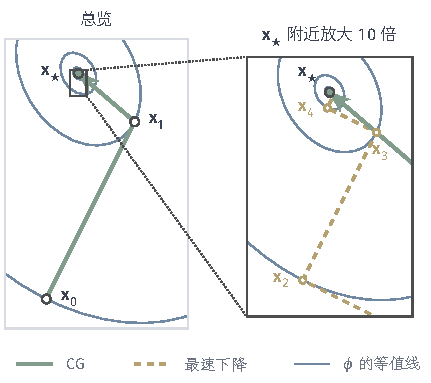
\includegraphics[width=72.873mm]{figures/01-basic-mathematics/03-vectors-matrices-and-multivariate-functions/tikz/c5-cg-steepest-descent-paths/figure.pdf}
  \caption{贯穿例上CG与最速下降的路径。蓝色椭圆是$\phi(\bm x)=\tfrac12\bm x^\top\bm A\bm x-\bm b^\top\bm x$经过最速下降各迭代点的等值线，中心为$\bm x_\star=(1/11,7/11)^\top$。两种方法的第一步都从$\bm x_0=\bm 0$走到$\bm x_1=(1/4,1/2)^\top$；CG的第二个方向与第一个方向$\bm A$共轭，直接指向椭圆中心，最速下降则在$\bm x_\star$附近来回折返（右图为左图小框放大10倍）。}
  \label{fig:ls-cg-steepest-descent-paths}
\end{figure}

\subsection{算法分析}

\paragraph{正确性与收敛速度}
正确性归结为两组关系：残差两两正交，方向两两共轭。由它们可以推出最优性，再由残差多项式得到收敛速度。

\begin{theorem}[CG的最优性与收敛速度]
\label{thm:ls-cg-convergence}
设$\bm A$对称正定，在精确算术下按上述递推计算，且$\bm r_0,\ldots,\bm r_{k-1}$均非零。则$\bm r_0,\ldots,\bm r_k$两两正交，$\bm p_0,\ldots,\bm p_{k-1}$两两关于$\bm A$共轭，$\bm x_k$是$\lVert\bm x-\bm x_\star\rVert_{\bm A}$在$\bm x_0+\mathcal K_k$上的唯一最小点，并且
\begin{equation}
 \lVert\bm x_k-\bm x_\star\rVert_{\bm A}\le2\Bigl(\frac{\sqrt\kappa-1}{\sqrt\kappa+1}\Bigr)^k\lVert\bm x_0-\bm x_\star\rVert_{\bm A},
 \label{eq:ls-cg-convergence-bound}
\end{equation}
其中$\kappa=\kappa_2(\bm A)$。CG至多$d$步得到精确解。
\end{theorem}

\begin{proof}
证明分三步：先证正交与共轭关系，再由它们推出最优性，最后估计收敛速度。

\emph{正交与共轭关系。}对$k$归纳证明：$\bm r_0,\ldots,\bm r_k$两两正交，$\bm p_0,\ldots,\bm p_k$两两共轭，且两组向量都张成$\mathcal K_{k+1}$。$k=0$时显然。设结论对$k$成立，先证$\bm r_{k+1}\perp\mathcal K_{k+1}$。由$\bm p_k=\bm r_k+\beta_{k-1}\bm p_{k-1}$及$\bm r_k\perp\bm p_{k-1}$，
\[
 \bm p_k^\top\bm r_k=\bm r_k^\top\bm r_k ,
\]
于是由步长~\eqref{eq:ls-cg-step}与残差更新~\eqref{eq:ls-cg-update}，
\[
 \bm p_k^\top\bm r_{k+1}=\bm p_k^\top\bm r_k-\alpha_k\bm p_k^\top\bm A\bm p_k=0 .
\]
对$i<k$，由归纳假设中的共轭性，
\[
 \bm p_i^\top\bm r_{k+1}=\bm p_i^\top\bm r_k-\alpha_k\bm p_i^\top\bm A\bm p_k=0 .
\]
$\bm p_0,\ldots,\bm p_k$张成$\mathcal K_{k+1}$，所以$\bm r_{k+1}\perp\mathcal K_{k+1}$，特别地与$\bm r_0,\ldots,\bm r_k$都正交。

再证$\bm p_{k+1}$与此前的方向共轭。对$i<k$，$\bm A\bm p_i\in\mathcal K_{i+2}\subseteq\mathcal K_{k+1}$，故$\bm r_{k+1}^\top\bm A\bm p_i=0$，从而
\[
 \bm p_{k+1}^\top\bm A\bm p_i=\bm r_{k+1}^\top\bm A\bm p_i+\beta_k\bm p_k^\top\bm A\bm p_i=0 .
\]
对$i=k$，由残差更新得$\bm A\bm p_k=(\bm r_k-\bm r_{k+1})/\alpha_k$，再用$\bm r_{k+1}\perp\bm r_k$与式~\eqref{eq:ls-cg-step}、\eqref{eq:ls-cg-beta}，
\[
 \bm r_{k+1}^\top\bm A\bm p_k=-\frac{\bm r_{k+1}^\top\bm r_{k+1}}{\alpha_k}=-\beta_k\,\bm p_k^\top\bm A\bm p_k ,
\]
恰被$\beta_k\bm p_k^\top\bm A\bm p_k$抵消，所以$\bm p_{k+1}^\top\bm A\bm p_k=0$。最后$\bm r_{k+1},\bm p_{k+1}\in\mathcal K_{k+2}$；若$\bm r_{k+1}\ne\bm 0$，两两正交的非零残差线性无关，两组向量都张成$\mathcal K_{k+2}$。

\emph{最优性。}记$\bm e_k=\bm x_k-\bm x_\star$，则$\bm A\bm e_k=-\bm r_k$，且由上一步$\bm r_k\perp\mathcal K_k$。对任意$\bm z\in\mathcal K_k$，
\[
 \lVert\bm e_k+\bm z\rVert_{\bm A}^2
 =\lVert\bm e_k\rVert_{\bm A}^2+2\bm z^\top\bm A\bm e_k+\lVert\bm z\rVert_{\bm A}^2
 =\lVert\bm e_k\rVert_{\bm A}^2+\lVert\bm z\rVert_{\bm A}^2 ,
\]
所以$\bm x_k$是$\bm x_0+\mathcal K_k$上的唯一最小点。$\mathbb R^d$中两两正交的非零向量至多$d$个，故至多$d$步出现零残差。

\emph{收敛速度。}按式~\eqref{eq:ls-krylov-residual-polynomial}的推导，$\bm x_0+\mathcal K_k$中候选的误差为$p(\bm A)\bm e_0$，其中$p\in\mathcal P_k$。由谱定理（定理~\ref{thm:ls-real-symmetric-spectral}）取标准正交特征向量展开$\bm e_0=\sum_ic_i\bm u_i$，得
\[
 \lVert p(\bm A)\bm e_0\rVert_{\bm A}^2=\sum_i\lambda_i\,p(\lambda_i)^2c_i^2\le\max_i p(\lambda_i)^2\,\lVert\bm e_0\rVert_{\bm A}^2 .
\]
由最优性，$\lVert\bm e_k\rVert_{\bm A}$不超过任一$p\in\mathcal P_k$给出的上界，只需构造一个在特征值上很小的$p$。取Chebyshev多项式$T_k$，它由$T_k(\cos\theta)=\cos k\theta$确定，在$[-1,1]$上$\lvert T_k\rvert\le1$；对$x>1$，
\[
 T_k(x)=\tfrac12\bigl[(x+\sqrt{x^2-1})^k+(x-\sqrt{x^2-1})^k\bigr],
\]
因为两边满足同一递推$T_{j+1}=2xT_j-T_{j-1}$和相同初值。令
\[
 \ell(t)=\frac{\lambda_{\max}+\lambda_{\min}-2t}{\lambda_{\max}-\lambda_{\min}},
\]
它把$[\lambda_{\min},\lambda_{\max}]$映到$[-1,1]$，且$\ell(0)=(\kappa+1)/(\kappa-1)$。取
\[
 p(t)=\frac{T_k(\ell(t))}{T_k(\ell(0))}\in\mathcal P_k ,
\]
则在各特征值处$\lvert p\rvert\le1/T_k(\ell(0))$。直接计算，$x=\ell(0)$时$x+\sqrt{x^2-1}=(\sqrt\kappa+1)/(\sqrt\kappa-1)$，于是
\[
 T_k(\ell(0))\ge\frac12\Bigl(\frac{\sqrt\kappa+1}{\sqrt\kappa-1}\Bigr)^k ,
\]
即得所述界。$\kappa=1$时$\bm A$是单位矩阵的倍数，一步得解。
\end{proof}

这个界只依赖两端特征值，误差缩小到给定比例所需的步数约与$\sqrt\kappa$成正比。它控制的是误差的$\bm A$范数，欧氏残差$\lVert\bm r_k\rVert_2$不必每步下降。

\paragraph{数值敏感度}
浮点计算中正交与共轭关系逐步受损，定理的有限步结论不能直接移用，实际计算不承诺恰好$d$步结束；递推残差也会偏离真实残差，所以宣布达到要求前按公共准则用$\bm b-\bm A\bm x_k$复核。

\paragraph{计算代价}
每轮核心递推需要一次$\bm A$乘向量、两次内积和三次向量更新。除矩阵外只保存$\bm x,\bm r,\bm p,\bm q$四个向量，存储不随步数增长；复核真实残差所需的矩阵乘向量另计。

\section{广义最小残差法}
\label{sec:ls-gmres}

设$\bm A$是一般的非奇异方阵，不要求对称或正定。\term{广义最小残差法}（generalized minimal residual method，GMRES）在第$k$步取$\bm x_0+\mathcal K_k$中使原残差长度$\lVert\bm b-\bm A\bm x\rVert_2$最小的近似，与MINRES同样采用第~\ref{sec:ls-krylov-selection-criteria}节的极小残差条件。它紧接第~\ref{sec:ls-arnoldi-application}节：Arnoldi正交化已把这一准则化为一个$(k+1)\times k$的上Hessenberg最小二乘问题，本节说明怎样随步数逐列求解它、怎样读出残差长度并还原近似解。Arnoldi递推本身不再重述，只引用第~\ref{sec:ls-arnoldi}节的式子与定理。

\subsection{主要思想}

\paragraph{逐步长大的小问题}
先看一个周期。记周期的起点为$\bm x^{(s)}$，残差为$\bm r^{(s)}=\bm b-\bm A\bm x^{(s)}$；不重启时只有一个周期，$\bm x^{(s)}=\bm x_0$。令
\begin{equation}
 \beta=\lVert\bm r^{(s)}\rVert_2,\qquad \bm v_1=\frac{\bm r^{(s)}}{\beta},
 \label{eq:ls-gmres-start}
\end{equation}
按式~\eqref{eq:ls-arnoldi-coefficients}与\eqref{eq:ls-arnoldi-normalize}作$j$轮Arnoldi正交化。由定理~\ref{thm:ls-arnoldi-relation}，$\bm V_{j+1}$的列标准正交，并有关系~\eqref{eq:ls-arnoldi-relation}：
\[
 \bm A\bm V_j=\bm V_{j+1}\overline{\bm H}_j .
\]
按第~\ref{sec:ls-arnoldi-application}节，候选写成$\bm x=\bm x^{(s)}+\bm V_j\bm y$，残差等于$\bm V_{j+1}(\beta\bm e_1-\overline{\bm H}_j\bm y)$，而$\bm V_{j+1}$不改变长度，所以
\begin{equation}
 \lVert\bm b-\bm A\bm x\rVert_2=\lVert\beta\bm e_1-\overline{\bm H}_j\bm y\rVert_2 .
 \label{eq:ls-gmres-small-problem}
\end{equation}
GMRES在每一步都要求出使右端最小的$\bm y$。

这个小问题随步数长大。第$j$步的$(j+1)\times j$上Hessenberg矩阵是
\[
 \overline{\bm H}_j=
 \begin{bmatrix}
 h_{1,1}&h_{1,2}&\cdots&h_{1,j-1}&h_{1,j}\\
 h_{2,1}&h_{2,2}&\cdots&h_{2,j-1}&h_{2,j}\\
 &h_{3,2}&\cdots&h_{3,j-1}&h_{3,j}\\
 &&\ddots&\vdots&\vdots\\
 &&&h_{j,j-1}&h_{j,j}\\
 &&&&h_{j+1,j}
 \end{bmatrix}.
\]
与MINRES一样，从第$j-1$步到第$j$步，矩阵只在右侧添了一列、在下方添了一行，已有元素不变。不同的是，新的一列$(h_{1,j},\ldots,h_{j+1,j})^\top$来自Arnoldi正交化中$\bm A\bm v_j$对全部旧基向量的系数，一般全都不为零；新的一行仍只有末元素$h_{j+1,j}$。所以前一步的消元结果仍可沿用，但处理新列的工作比MINRES多。

\paragraph{沿用前一步的消元结果}
小问题用第~\ref{sec:ls-qr-method}节的Givens旋转化为上三角。第$i$个旋转$\bm G_i$只作用于第$i$、$i+1$两行，在这两行上的形式为
\[
 \begin{bmatrix}c_i&s_i\\-s_i&c_i\end{bmatrix},\qquad c_i^2+s_i^2=1 ,
\]
用来消去第$i$列的次对角元。设前$j-1$步已经用$\bm G_1,\ldots,\bm G_{j-1}$把$\overline{\bm H}_{j-1}$消成了上三角，记所得上三角矩阵的元素为$r_{i,l}$。由于$\overline{\bm H}_{j-1}$的各列一般都是满的，这个上三角矩阵也是满的。以$j=4$为例，前三列经过$\bm G_1,\bm G_2,\bm G_3$后成为
\[
 \begin{bmatrix}
 r_{1,1}&r_{1,2}&r_{1,3}\\
 0&r_{2,2}&r_{2,3}\\
 0&0&r_{3,3}\\
 0&0&0
 \end{bmatrix}.
\]
以后的旋转只作用于第$4$行及以下，这三列不再改变。

\paragraph{新列要经过全部旧旋转}
前$j-1$列已经过$\bm G_1,\ldots,\bm G_{j-1}$，新列必须也依次经过这些旧旋转，整个矩阵才是同一个正交变换的结果。新列在第$1$至$j+1$行都可能非零，所以每个旧旋转都会改变它，不能像MINRES那样只用最近两个。旧旋转作用完后，新列在对角线以下只剩第$j+1$行的$h_{j+1,j}$，再构造一个新旋转$\bm G_j$把它消去。

以$j=4$为例，新列逐次旋转的变化为
\[
 \begin{bmatrix}h_{1,4}\\h_{2,4}\\h_{3,4}\\h_{4,4}\\h_{5,4}\end{bmatrix}
 \xrightarrow{\ \bm G_1\ }
 \begin{bmatrix}r_{1,4}\\\ast\\h_{3,4}\\h_{4,4}\\h_{5,4}\end{bmatrix}
 \xrightarrow{\ \bm G_2\ }
 \begin{bmatrix}r_{1,4}\\r_{2,4}\\\ast\\h_{4,4}\\h_{5,4}\end{bmatrix}
 \xrightarrow{\ \bm G_3\ }
 \begin{bmatrix}r_{1,4}\\r_{2,4}\\r_{3,4}\\a\\h_{5,4}\end{bmatrix}
 \xrightarrow{\ \bm G_4\ }
 \begin{bmatrix}r_{1,4}\\r_{2,4}\\r_{3,4}\\\rho_4\\0\end{bmatrix},
\]
其中$\ast$表示被旋转改动、随即又被下一个旋转改动的中间值，$a$是第$4$行在旧旋转作用完后的元素。每个旧旋转$\bm G_i$把第$i$、$i+1$两个分量换成
\[
 \begin{bmatrix}c_i&s_i\\-s_i&c_i\end{bmatrix}
 \begin{bmatrix}h_{i,j}\\h_{i+1,j}\end{bmatrix},
\]
第$i$个分量就此定下，成为$r_{i,j}$。整个矩阵在新旋转之前与之后分别是
\[
 \begin{bmatrix}
 r_{1,1}&r_{1,2}&r_{1,3}&r_{1,4}\\
 0&r_{2,2}&r_{2,3}&r_{2,4}\\
 0&0&r_{3,3}&r_{3,4}\\
 0&0&0&a\\
 0&0&0&h_{5,4}
 \end{bmatrix}
 \xrightarrow{\ \bm G_4\ }
 \begin{bmatrix}
 r_{1,1}&r_{1,2}&r_{1,3}&r_{1,4}\\
 0&r_{2,2}&r_{2,3}&r_{2,4}\\
 0&0&r_{3,3}&r_{3,4}\\
 0&0&0&\rho_4\\
 0&0&0&0
 \end{bmatrix}.
\]
新旋转只处理右下角的$a$与$h_{5,4}$。一般地，记$h=h_{j+1,j}$，新旋转取
\begin{equation}
 \rho_j=\sqrt{a^2+h^2},\qquad c_j=\frac a{\rho_j},\qquad s_j=\frac h{\rho_j},
 \label{eq:ls-gmres-givens}
\end{equation}
把$(a,h)$变为$(\rho_j,0)$，$\rho_j=r_{j,j}$；实际用不会溢出的$\operatorname{hypot}(a,h)$计算$\rho_j$。旋转都要保存下来，供以后各列使用。

\paragraph{右端与残差}
同一组旋转也作用于右端$\beta\bm e_1$。它的第$j+1$个分量起初为零，只有第$j$个旋转才把非零值带下来；记右端为$\bm g$，初值$\bm g=\beta\bm e_1$，则
\begin{equation}
 g_j\leftarrow c_jg_j,\qquad g_{j+1}=-s_jg_j ,
 \label{eq:ls-gmres-rhs}
\end{equation}
右边都用旋转前的$g_j$，前面已确定的分量不变。以$j=4$为例，右端在$\bm G_4$前后分别是
\[
 \begin{bmatrix}g_1\\g_2\\g_3\\g_4\\0\end{bmatrix}
 \xrightarrow{\ \bm G_4\ }
 \begin{bmatrix}g_1\\g_2\\g_3\\c_4g_4\\-s_4g_4\end{bmatrix}.
\]
全部$j$个旋转作用后，小矩阵成为上三角块$\bm R_j$下接一行零。旋转保长，小问题的目标化为
\begin{equation}
 \lVert\beta\bm e_1-\overline{\bm H}_j\bm y\rVert_2^2
 =\lVert(g_1,\ldots,g_j)^\top-\bm R_j\bm y\rVert_2^2+g_{j+1}^2 .
 \label{eq:ls-gmres-rotated-objective}
\end{equation}
前$j$个方程可由上三角的$\bm R_j$精确满足，最后一个分量$g_{j+1}$无论$\bm y$取什么都无法消去，所以最小残差长度就是$\lvert g_{j+1}\rvert$。由式~\eqref{eq:ls-gmres-rhs}，它满足
\[
 \lvert g_{j+1}\rvert=\lvert s_j\rvert\,\lvert g_j\rvert\le\lvert g_j\rvert ,
\]
因而随步数不增。不形成$\bm y$和$\bm x$，每步就能读出残差长度，用来决定何时停下。

\paragraph{与MINRES的差别}
消元的框架与MINRES相同，残差长度也同样随消元得到；差别都来自新列是满的。

其一，每步的工作量随步数增长：第$j$步要作用$j-1$个旧旋转，Arnoldi正交化还要与$j$个旧基向量求内积并扣除，全部旋转与基向量都须保存。

其二，没有短递推。MINRES的$\bm R_k$只有三条非零对角线，可以把$\bm V_k\bm R_k^{-1}$的列写成方向的三项递推，边迭代边累加解；这里$\bm R_j$是满的上三角矩阵，新方向要与全部旧方向组合，而且每增加一列，回代所得$\bm y$的各个分量一般都会改变。所以GMRES不逐步更新$\bm x$，只在停下时由回代
\begin{equation}
 \bm R_j\bm y=(g_1,\ldots,g_j)^\top
 \label{eq:ls-gmres-back-substitution}
\end{equation}
求出系数，再由
\begin{equation}
 \bm x=\bm x^{(s)}+\bm V_j\bm y
 \label{eq:ls-gmres-solution}
\end{equation}
用整组基还原原变量。这组基本来也要用于Arnoldi的扣除，保存它并不额外增加存储。

$\bm A$对称时，由第~\ref{sec:ls-lanczos}节，$\overline{\bm H}_j$成为三对角矩阵，新列只有三个非零元，只需经过两个旧旋转，回代也化为短递推，这就是第~\ref{sec:ls-minres}节的MINRES。

\paragraph{重启}
基的存储与正交化工作都随步数增长，实际常用重启：每个周期最多走$m$步，按式~\eqref{eq:ls-gmres-solution}更新$\bm x$，用原矩阵重算残差，再以它为新周期的$\bm r^{(s)}$重新生成基。重启限制了存储，代价是新周期不再利用旧周期的子空间。

\subsection{算法实现}

输入为非奇异方阵$\bm A$与右端$\bm b$，算法只需计算$\bm A$乘向量，输出为近似解$\bm x$。预先选定初值$\bm x_0$、容差$\mathrm{atol},\mathrm{rtol}$、总步数上限$K$与重启长度$m$（$1\le m\le d$）；停止阈值$\tau$与执行流程沿用第~\ref{sec:ls-matrix-splitting}节，各种结束原因的含义见第~\ref{sec:ls-stationary-stopping}节。

按上一小节的推导，每轮作一轮Arnoldi扩展，让新列经过全部旧旋转，再构造一个新旋转并更新右端，由$\lvert g_{j+1}\rvert$判断是否停下；停下后回代、还原，并从真实残差决定是否重启。下面写出计算中用到的变量、它们怎样初始化、每轮怎样更新。每一步使用例~\ref{ex:ls-stationary-running-example}的数据进行演示，取$m=2$：
\[
 \bm A=\begin{bmatrix}4&1\\1&3\end{bmatrix},\qquad
 \bm b=\begin{bmatrix}1\\2\end{bmatrix},\qquad
 \bm x_0=\bm 0 .
\]
Arnoldi部分的数值与第~\ref{sec:ls-arnoldi}节相同。

\paragraph{变量}
\begin{itemize}
 \item $\bm x^{(s)}\in\mathbb R^d$：本周期的起点，周期结束时更新为新的近似解。
 \item $\bm v_1,\ldots,\bm v_{j+1}\in\mathbb R^d$：本周期的标准正交基，全部保存，回代后用来还原解。
 \item $\bm w\in\mathbb R^d$：Arnoldi的工作向量。
 \item $h_{1,j},\ldots,h_{j+1,j}$：$\overline{\bm H}_j$的第$j$列；经旋转后在原处变为$\bm R_j$的第$j$列，对角元为$\rho_j$，次对角元变为零。
 \item $c_i,s_i$（$i\le j$）：已构造的旋转，全部保存。
 \item $\bm g\in\mathbb R^{j+1}$：经旋转的右端，前$j$个分量用于回代，$\lvert g_{j+1}\rvert$是残差长度的估计。
 \item $j$：本周期内的轮次；另记累计步数，与上限$K$比较。
\end{itemize}

\paragraph{初始化}
把周期起点初始化为$\bm x_0$，计算残差并作停止检查：$\lVert\bm r^{(s)}\rVert_2\le\tau$时以“达到容差”结束，累计步数已达$K$时以“步数耗尽”结束，都输出$\bm x^{(s)}$，不再归一化。否则把第一个基向量初始化为残差的方向，右端初始化为$\beta\bm e_1$，轮次初始化为$1$：
\[
 \begin{gathered}
 \bm x^{(s)}=\bm x_0,\qquad \bm r^{(s)}=\bm b-\bm A\bm x^{(s)},\qquad \beta=\lVert\bm r^{(s)}\rVert_2,\\
 \bm v_1=\frac{\bm r^{(s)}}{\beta},\qquad \bm g=\beta\bm e_1,\qquad j=1 .
 \end{gathered}
\]
重启时以新的$\bm x^{(s)}$回到这里，所以这里的停止检查用的总是原矩阵重算的真实残差。例中$\bm r^{(s)}=\bm b$，
\[
 \beta=\sqrt5,\qquad \bm v_1=\frac1{\sqrt5}\begin{bmatrix}1\\2\end{bmatrix},\qquad \bm g=\begin{bmatrix}\sqrt5\\0\end{bmatrix}.
\]

\paragraph{每轮更新}
在第$j$轮：
\begin{enumerate}
 \item \textbf{Arnoldi扩展。}按第~\ref{sec:ls-arnoldi}节计算过程中每轮更新的第1—3步，即式~\eqref{eq:ls-arnoldi-coefficients}与\eqref{eq:ls-arnoldi-normalize}，计算
 \[
  \begin{gathered}
  \bm w=\bm A\bm v_j ,\\
  h_{i,j}=\bm v_i^\top\bm w,\qquad \bm w\leftarrow\bm w-h_{i,j}\bm v_i\qquad(i=1,\ldots,j),\\
  h_{j+1,j}=\lVert\bm w\rVert_2,\qquad \bm v_{j+1}=\frac{\bm w}{h_{j+1,j}} ,
  \end{gathered}
 \]
 得到$\overline{\bm H}_j$的新列；$h_{j+1,j}=0$时不作归一化，不生成$\bm v_{j+1}$。必要时按该节的办法再正交化。例中第一轮
 \[
  \bm A\bm v_1=\frac1{\sqrt5}\begin{bmatrix}6\\7\end{bmatrix},\qquad
  \begin{bmatrix}h_{1,1}\\h_{2,1}\end{bmatrix}=\begin{bmatrix}4\\1\end{bmatrix},\qquad
  \bm v_2=\frac1{\sqrt5}\begin{bmatrix}2\\-1\end{bmatrix}.
 \]

 \item \textbf{作用旧旋转。}对$i=1,\ldots,j-1$依次计算
 \begin{equation}
  \begin{bmatrix}h_{i,j}\\h_{i+1,j}\end{bmatrix}\leftarrow
  \begin{bmatrix}c_i&s_i\\-s_i&c_i\end{bmatrix}\begin{bmatrix}h_{i,j}\\h_{i+1,j}\end{bmatrix},
  \label{eq:ls-gmres-old-rotations}
 \end{equation}
 每次只改动相邻的两个元素。例中第一轮没有旧旋转，新列仍为$(4,1)^\top$。

 \item \textbf{构造新旋转。}取$a=h_{j,j}$、$h=h_{j+1,j}$，按式~\eqref{eq:ls-gmres-givens}算出$\rho_j,c_j,s_j$并保存，令$h_{j,j}\leftarrow\rho_j$、$h_{j+1,j}\leftarrow0$。$h_{j+1,j}=0$时$s_j=0$，照常完成本列；若$a=h=0$，则$\rho_j=0$，小问题秩亏，要先检查$\bm A$是否奇异、小问题是否相容，不能直接相除。例中第一轮$a=4$、$h=1$，
 \[
  \rho_1=\sqrt{17},\qquad c_1=\frac4{\sqrt{17}},\qquad s_1=\frac1{\sqrt{17}} .
 \]

 \item \textbf{更新右端。}按式~\eqref{eq:ls-gmres-rhs}计算
 \[
  g_{j+1}=-s_jg_j,\qquad g_j\leftarrow c_jg_j ,
 \]
 $\lvert g_{j+1}\rvert$即本轮的残差估计。例中第一轮
 \[
  \bm g=\frac{\sqrt5}{\sqrt{17}}\begin{bmatrix}4\\-1\end{bmatrix},\qquad \lvert g_2\rvert=\sqrt{\frac5{17}}\approx0.542 .
 \]

 \item \textbf{停止。}若$\lvert g_{j+1}\rvert\le\tau$，或第1步给出$h_{j+1,j}=0$（这时$g_{j+1}=0$），或本周期已走$m$轮，或累计步数达到$K$，退出每轮更新，转入回代；否则令$j\leftarrow j+1$，进入下一轮。$\lvert g_{j+1}\rvert$只是小问题上的估计，是否真正结束要在回代、还原之后由初始化中的真实残差检查决定，见第~\ref{sec:ls-stationary-stopping}节。

 例中第一轮$0.542$未达标，$j=1<m$，进入第二轮。若在此退出，回代得
 \[
  y_1=\frac{g_1}{\rho_1}=\frac{4\sqrt5}{17},\qquad
  \bm x_1=y_1\bm v_1=\begin{bmatrix}4/17\\8/17\end{bmatrix},
 \]
 与MINRES的第一步相同。

 第二轮由第1步，$\bm A\bm v_2=(7,-1)^\top/\sqrt5$，
 \[
  h_{1,2}=1,\qquad h_{2,2}=3,\qquad h_{3,2}=0 ;
 \]
 由第2步，前两个元素经$\bm G_1$变为
 \[
  \begin{bmatrix}c_1&s_1\\-s_1&c_1\end{bmatrix}\begin{bmatrix}1\\3\end{bmatrix}
  =\frac1{\sqrt{17}}\begin{bmatrix}7\\11\end{bmatrix};
 \]
 由第3、4步，$a=11/\sqrt{17}$、$h=0$，
 \[
  \rho_2=\frac{11}{\sqrt{17}},\qquad c_2=1,\qquad s_2=0,\qquad g_3=0 ,
 \]
 $g_2$不变。第二轮$h_{3,2}=0$，二维空间已经用尽，退出每轮更新。
\end{enumerate}

\paragraph{回代与重启}
退出后，旋转过的各列组成上三角矩阵$\bm R_j$，按式~\eqref{eq:ls-gmres-back-substitution}自下而上回代求$\bm y$，再按式~\eqref{eq:ls-gmres-solution}还原$\bm x$。然后令$\bm x^{(s)}\leftarrow\bm x$，回到初始化：在那里用原矩阵重算残差并复核，满足阈值或已达累计步数上限就输出，否则从这个残差开始新的周期。若几个周期后真实残差几乎不再下降，应报告停滞，而不是继续无限重启。

例中两轮的结果组成
\[
 \bm R_2=\frac1{\sqrt{17}}\begin{bmatrix}17&7\\0&11\end{bmatrix},\qquad
 (g_1,g_2)^\top=\frac{\sqrt5}{\sqrt{17}}\begin{bmatrix}4\\-1\end{bmatrix},
\]
回代得
\[
 y_2=-\frac{\sqrt5}{11},\qquad y_1=\frac{4\sqrt5-7y_2}{17}=\frac{3\sqrt5}{11},
\]
于是
\[
 \bm x=\bm V_2\bm y=\frac3{11}\begin{bmatrix}1\\2\end{bmatrix}-\frac1{11}\begin{bmatrix}2\\-1\end{bmatrix}=\begin{bmatrix}\tfrac1{11}\\\tfrac7{11}\end{bmatrix}.
\]

最终得到本周期子空间中残差最小的近似解。例中回到初始化后真实残差为零，以“达到容差”结束，输出
\[
 \bm x_\star=\begin{bmatrix}\tfrac1{11}\\\tfrac7{11}\end{bmatrix} .
\]
代回核对：
\[
 \bm A\bm x_\star=\begin{bmatrix}4/11+7/11\\1/11+21/11\end{bmatrix}=\begin{bmatrix}1\\2\end{bmatrix}=\bm b ,
\]
与MINRES的结果相同；$\bm R_2$与$\bm g$也正是把第~\ref{sec:ls-arnoldi}节的$\overline{\bm H}_2$与$\sqrt5\,\bm e_1$用同两个旋转变换的结果。

贯穿例的矩阵是对称的，小矩阵也对称。下面换用非对称矩阵，这是MINRES不再适用、GMRES仍然可用的情形。

\begin{example}[非对称矩阵上的GMRES]
\label{ex:ls-gmres-nonsymmetric}
下面用以下数据演示，取$m=2$：
\[
 \bm A=\begin{bmatrix}3&1\\0&2\end{bmatrix},\qquad
 \bm b=\begin{bmatrix}1\\1\end{bmatrix},\qquad
 \bm x_0=\bm0 .
\]
于是$\bm r_0=\bm b$，$\beta=\sqrt2$，$\bm v_1=(1,1)^\top/\sqrt2$。

第一轮由第1步，$\bm A\bm v_1=(4,2)^\top/\sqrt2$，得新列与新基向量
\[
 \begin{bmatrix}h_{1,1}\\h_{2,1}\end{bmatrix}=\begin{bmatrix}3\\1\end{bmatrix},\qquad
 \bm v_2=\frac1{\sqrt2}\begin{bmatrix}1\\-1\end{bmatrix}.
\]
由第3、4步，
\[
 \rho_1=\sqrt{10},\qquad c_1=\frac3{\sqrt{10}},\qquad s_1=\frac1{\sqrt{10}},\qquad
 \bm g=\frac1{\sqrt5}\begin{bmatrix}3\\-1\end{bmatrix}.
\]
若在此结束，回代得
\[
 y_1=\frac{3\sqrt2}{10},\qquad \bm x_1=y_1\bm v_1=\begin{bmatrix}3/10\\3/10\end{bmatrix}.
\]
直接计算原残差
\[
 \bm r_1=\bm b-\bm A\bm x_1=\begin{bmatrix}-1/5\\2/5\end{bmatrix},\qquad
 \lVert\bm r_1\rVert_2=\frac1{\sqrt5}=\lvert g_2\rvert .
\]

第二轮$\bm A\bm v_2=2\bm v_2$，新列为$(0,2,0)^\top$，与对角线下方的$h_{2,1}=1$不对称。由第2步，它经$\bm G_1$变为
\[
 \begin{bmatrix}2/\sqrt{10}\\6/\sqrt{10}\\0\end{bmatrix};
\]
由于$h_{3,2}=0$，新旋转为$c_2=1$、$s_2=0$，$g_3=0$。回代
\[
 \begin{bmatrix}\sqrt{10}&2/\sqrt{10}\\0&6/\sqrt{10}\end{bmatrix}\begin{bmatrix}y_1\\y_2\end{bmatrix}=\frac1{\sqrt5}\begin{bmatrix}3\\-1\end{bmatrix}
\]
得$y_2=-\sqrt2/6$、$y_1=\sqrt2/3$，恢复出
\[
 \bm x_2=\frac13\begin{bmatrix}1\\1\end{bmatrix}-\frac16\begin{bmatrix}1\\-1\end{bmatrix}=\begin{bmatrix}\tfrac16\\\tfrac12\end{bmatrix},
\]
代回得$\bm A\bm x_2=(1/2+1/2,\,1)^\top=\bm b$，原残差为零。两轮中的Arnoldi系数可以按第~\ref{sec:ls-arnoldi}节的计算过程逐步核对。
\end{example}

\subsection{算法分析}

\paragraph{正确性}
下面的定理针对不重启的完整GMRES，即$m=d$、$\bm x^{(s)}=\bm x_0$的情形。

\begin{theorem}[GMRES的最小残差性]
\label{thm:ls-gmres-optimality}
设$\bm A$非奇异，在精确算术下执行完整GMRES的第$k$步，记$\bm r_k=\bm b-\bm A\bm x_k$。则$\bm x_k$是$\bm x_0+\mathcal K_k$中残差长度的唯一最小点，$\lVert\bm r_k\rVert_2=\lvert g_{k+1}\rvert$，它等于上一步的残差长度乘以$\lvert s_k\rvert\le1$，因而随$k$不增；GMRES至多$d$步得到精确解。若$\bm A=\bm X\bm\Lambda\bm X^{-1}$可对角化（$\bm X,\bm\Lambda$可以是复矩阵），还有
\begin{equation}
 \lVert\bm r_k\rVert_2\le\kappa_2(\bm X)\min_{p\in\mathcal P_k}\max_{\lambda\in\sigma(\bm A)}\lvert p(\lambda)\rvert\,\lVert\bm r_0\rVert_2,
 \label{eq:ls-gmres-residual-bound}
\end{equation}
其中$\mathcal P_k$同引理~\ref{lem:ls-krylov-residual-polynomial}。
\end{theorem}

\begin{proof}
证明分四步：先把原问题化为小问题，再由旋转求出小问题的解与最小值，然后说明单调性与有限步终止，最后由残差多项式得到界。

\emph{化为小问题。}由Arnoldi关系（定理~\ref{thm:ls-arnoldi-relation}），Arnoldi尚未停止时$\bm V_{k+1}$的列标准正交，且$\bm A\bm V_k=\bm V_{k+1}\overline{\bm H}_k$。由$\bm r_0=\beta\bm V_{k+1}\bm e_1$，
\[
 \bm b-\bm A(\bm x_0+\bm V_k\bm y)=\bm r_0-\bm A\bm V_k\bm y=\bm V_{k+1}(\beta\bm e_1-\overline{\bm H}_k\bm y),
\]
乘以$\bm V_{k+1}$不改变长度，即得式~\eqref{eq:ls-gmres-small-problem}。$\bm V_k$满列秩，$\bm y\mapsto\bm x_0+\bm V_k\bm y$是$\mathbb R^k$到$\bm x_0+\mathcal K_k$的双射，两个最小化问题的解一一对应。

\emph{旋转后的小问题。}记$k$个旋转之积为正交矩阵$\bm\Omega_k$。每个新旋转只作用于第$j,j+1$行，而新列在此前已经过全部旧旋转，所以
\[
 \bm\Omega_k\overline{\bm H}_k=\begin{bmatrix}\bm R_k\\\bm 0^\top\end{bmatrix},\qquad
 \bm\Omega_k\beta\bm e_1=\bm g=(g_1,\ldots,g_{k+1})^\top ,
\]
从而
\[
 \lVert\beta\bm e_1-\overline{\bm H}_k\bm y\rVert_2^2
 =\lVert(g_1,\ldots,g_k)^\top-\bm R_k\bm y\rVert_2^2+g_{k+1}^2 .
\]
$\bm A$非奇异且$\bm V_k$满列秩，$\bm A\bm V_k=\bm V_{k+1}\overline{\bm H}_k$满列秩，故$\overline{\bm H}_k$与$\bm R_k$满秩，$\bm R_k$可逆。回代~\eqref{eq:ls-gmres-back-substitution}所得的$\bm y$使第一项为零，且是唯一使之为零的点，最小值为$\lvert g_{k+1}\rvert$。

\emph{单调性与有限步终止。}第$k$个旋转把旋转前的$g_k$变为$c_kg_k$与$-s_kg_k$，而旋转前的$\lvert g_k\rvert$正是上一步的残差长度，所以
\[
 \lvert g_{k+1}\rvert=\lvert s_k\rvert\,\lvert g_k\rvert\le\lvert g_k\rvert .
\]
若$h_{k+1,k}=0$，则$s_k=0$，$g_{k+1}=0$，残差为零；子空间维数不超过$d$，所以至多$d$步出现这一情形或零残差。

\emph{残差界。}由引理~\ref{lem:ls-krylov-residual-polynomial}与最小残差性，
\[
 \lVert\bm r_k\rVert_2=\min_{p\in\mathcal P_k}\lVert p(\bm A)\bm r_0\rVert_2 .
\]
而$p(\bm A)=\bm X\,p(\bm\Lambda)\bm X^{-1}$，对角矩阵$p(\bm\Lambda)$的谱范数是$\max_{\lambda\in\sigma(\bm A)}\lvert p(\lambda)\rvert$，于是
\[
 \lVert p(\bm A)\bm r_0\rVert_2\le\lVert\bm X\rVert_2\lVert\bm X^{-1}\rVert_2\max_{\lambda\in\sigma(\bm A)}\lvert p(\lambda)\rvert\,\lVert\bm r_0\rVert_2 ,
\]
其中$\lVert\bm X\rVert_2\lVert\bm X^{-1}\rVert_2=\kappa_2(\bm X)$，对$p$取最小即得所述界。
\end{proof}

\paragraph{收敛速度}
定理中的界把收敛问题化为多项式逼近：要找在原点取值$1$、在全部特征值上都很小的低次多项式。非正规矩阵的$\kappa_2(\bm X)$可能很大，界因此变弱，只看特征值是否集中不能判断收敛快慢。

\paragraph{重启与数值敏感度}
重启的GMRES($m$)丢弃了历史空间：每个周期内的残差仍最小，但这只是在本周期子空间上的最优，不能说成累计全部历史空间上的最优。它可能停滞，也不再有$d$步得到精确解的保证。浮点计算中基不再精确正交，$\lvert g_{j+1}\rvert$与真实残差会偏离，这就是每个周期结束时用$\bm b-\bm A\bm x$复核的原因。

\paragraph{计算代价}
每轮需要一次$\bm A$乘向量。完整GMRES执行$k$步时，正交化共约$2dk^2$次浮点运算，基的存储约$kd$个数，都随步数增长；GMRES($m$)把历史基限制在一个周期内，每周期至多约$2dm^2$次运算，存储约$(m+1)d$个数，与总步数无关。

\section{双共轭梯度法}
\label{sec:ls-bicg}

第~\ref{sec:ls-arnoldi-application}节说明，对一般方阵，Arnoldi正交化给出的小问题无论按Galerkin条件还是按极小残差条件求解，都要用整组基还原近似解；GMRES（第~\ref{sec:ls-gmres}节）因此须保存全部基向量，存储与正交化工作随步数线性增长。

第~\ref{sec:ls-lanczos-application}节的短递推则依赖对称性：正是$\bm A^\top=\bm A$使大部分系数$h_{i,j}$为零，MINRES与CG才只需固定数量的向量。

本节的双共轭梯度法针对一般的非对称可逆方阵，改用第~\ref{sec:ls-krylov-selection-criteria}节第四类准则中的影子空间：残差不再与$\mathcal K_k$本身正交，而与$\bm A^\top$生成的Krylov子空间正交，即Petrov--Galerkin条件~\eqref{eq:ls-krylov-projection}。这样恢复了短递推，算法形式与CG的式~\eqref{eq:ls-cg-update}—\eqref{eq:ls-cg-beta}相仿，代价是放弃残差的最小化；下一节的BiCGSTAB在此基础上减缓残差的起伏。

\subsection{主要思想}

设$\bm A$是一般的实可逆方阵，不要求对称。

\paragraph{影子空间}
对一般的非对称矩阵，在单一的Krylov子空间$\mathcal K_k(\bm A,\bm r_0)$中，短递推与最优性一般不能兼得：GMRES保住了残差最小，却要保存整组基；Lanczos过程的短递推则依赖$\bm A^\top=\bm A$。

BiCG的做法是放弃最优性、保住短递推。为此，除了原方程$\bm A\bm x=\bm b$，它还引入一个以$\bm A^\top$为系数的影子方程，从满足$\widetilde{\bm r}_0^\top\bm r_0\ne0$的影子残差$\widetilde{\bm r}_0$出发，生成影子空间$\mathcal K_k(\bm A^\top,\widetilde{\bm r}_0)$。近似仍取在$\bm x_0+\mathcal K_k(\bm A,\bm r_0)$中，但要求残差与影子空间正交：
\[
 \bm r_k\perp\mathcal K_k(\bm A^\top,\widetilde{\bm r}_0),
\]
即第~\ref{sec:ls-krylov-selection-criteria}节的Petrov--Galerkin条件~\eqref{eq:ls-krylov-projection}。\term{双共轭梯度法}（biconjugate gradient method，BiCG）就按这一条件选取近似。下面看这个条件怎样化成一个三对角方程，以及怎样像CG那样逐步求解它。

\paragraph{双正交的两组基}
设$\bm V_k$的列$\bm v_1,\ldots,\bm v_k$是$\mathcal K_k(\bm A,\bm r_0)$的一组基，$\bm W_k$的列$\bm w_1,\ldots,\bm w_k$是$\mathcal K_k(\bm A^\top,\widetilde{\bm r}_0)$的一组基，且两者的前$j$列分别张成$\mathcal K_j(\bm A,\bm r_0)$与$\mathcal K_j(\bm A^\top,\widetilde{\bm r}_0)$。第~\ref{sec:ls-lanczos}节推导三项递推时，用对称性把$\bm v_i^\top\bm A\bm v_j$改写为$(\bm A\bm v_i)^\top\bm v_j$；没有对称性时，转置把$\bm A$换成$\bm A^\top$，
\[
 \bm w_i^\top\bm A\bm v_j=(\bm A^\top\bm w_i)^\top\bm v_j ,
\]
而$\bm A^\top\bm w_i$正好留在影子空间中。于是要求两组基\term{双正交}（biorthogonality），并归一化为
\begin{equation}
 \bm w_i^\top\bm v_j=\begin{cases}1,&i=j,\\0,&i\ne j,\end{cases}\qquad\text{即}\quad \bm W_k^\top\bm V_k=\bm I .
 \label{eq:ls-bicg-biorthonormal}
\end{equation}
这时$\bm v_j$与$\mathcal K_{j-1}(\bm A^\top,\widetilde{\bm r}_0)$正交，$\bm w_i$与$\mathcal K_{i-1}(\bm A,\bm r_0)$正交。又因为
\[
 \bm A^\top\bm w_i\in\mathcal K_{i+1}(\bm A^\top,\widetilde{\bm r}_0),\qquad \bm A\bm v_j\in\mathcal K_{j+1}(\bm A,\bm r_0),
\]
所以
\[
 \bm w_i^\top\bm A\bm v_j=0\qquad(\lvert i-j\rvert>1),
\]
因此投影矩阵$\bm T_k=\bm W_k^\top\bm A\bm V_k$是三对角的，但一般不对称。

记它的对角元为$a_j$、次对角元为$\gamma_j$、上对角元为$\eta_j$，以$k=3$为例，
\[
 \bm T_3=\begin{bmatrix}a_1&\eta_1&0\\\gamma_1&a_2&\eta_2\\0&\gamma_2&a_3\end{bmatrix}.
\]
与Lanczos过程一样，这两组基可以用三项递推交替生成：
\begin{equation}
 \begin{gathered}
 \bm A\bm v_j=\eta_{j-1}\bm v_{j-1}+a_j\bm v_j+\gamma_j\bm v_{j+1},\\
 \bm A^\top\bm w_j=\gamma_{j-1}\bm w_{j-1}+a_j\bm w_j+\eta_j\bm w_{j+1},
 \end{gathered}
 \label{eq:ls-bicg-two-sided-lanczos}
\end{equation}
每个新基向量只需扣除两个旧方向，称为双边Lanczos过程。若某一步扣除后的两个余项内积为零而余项本身不为零，就无法归一化，递推中断。

\paragraph{逐步长大的三对角方程}
取$\bm v_1=\bm r_0/\beta$，$\beta=\lVert\bm r_0\rVert_2$，并取$\bm w_1$与$\widetilde{\bm r}_0$同向、满足$\bm w_1^\top\bm v_1=1$。把近似写成
\[
  \bm x_k=\bm x_0+\bm V_k\bm y_k ,
\]
Petrov--Galerkin条件是
\[
  \bm W_k^\top(\bm r_0-\bm A\bm V_k\bm y_k)=\bm 0 .
\]
由$\bm W_k^\top\bm V_k=\bm I$得
\[
  \bm W_k^\top\bm r_0=\beta\bm e_1 ,
\]
于是条件化为$k$阶三对角方程
\begin{equation}
 \bm T_k\bm y_k=\beta\bm e_1 .
 \label{eq:ls-bicg-tridiagonal-system}
\end{equation}

这与CG的处境完全相同：每一步$\bm T_k$只在右侧添一列、在下方添一行，新添的元素只有$\eta_{k-1},\gamma_{k-1},a_k$。区别只在于$\bm T_k$不对称，也不一定正定。

\paragraph{分解的增量更新}
不对称的三对角矩阵不能作$\bm L\bm D\bm L^\top$分解，改作不选主元的LU分解：
\[
 \bm T_k=\bm L_k\bm U_k ,
\]
其中$\bm L_k$是单位下双对角矩阵，次对角元记为$\ell_j$；$\bm U_k$是上双对角矩阵，对角元记为$d_j$。

以$k=3$为例，
\[
 \bm L_3\bm U_3=
 \begin{bmatrix}1&&\\\ell_1&1&\\&\ell_2&1\end{bmatrix}
 \begin{bmatrix}d_1&\eta_1&\\&d_2&\eta_2\\&&d_3\end{bmatrix}
 =\begin{bmatrix}d_1&\eta_1&\\\ell_1d_1&\ell_1\eta_1+d_2&\eta_2\\&\ell_2d_2&\ell_2\eta_2+d_3\end{bmatrix}.
\]
$\bm U_k$的上对角元就是$\bm T_k$的$\eta_j$。

与$\bm T_3$逐元素比较，从$d_1=a_1$出发，逐个算出
\begin{equation}
 \ell_j=\frac{\gamma_j}{d_j},\qquad d_{j+1}=a_{j+1}-\ell_j\eta_j\qquad(j=1,2,\ldots).
 \label{eq:ls-bicg-lu}
\end{equation}
对称时$\eta_j=\gamma_j$，这就是CG的式~\eqref{eq:ls-cg-ldl}。与CG一样，$\bm T_{k+1}$只多出$\eta_k,\gamma_k,a_{k+1}$，$\bm L_k,\bm U_k$原封不动，只需在末尾追加$\ell_k$与$d_{k+1}$。不同的是，这里没有正定性保证$d_j\ne0$；若某个$d_j=0$，不选主元的LU就无法继续，这是BiCG的另一种中断。

\paragraph{翻译回向量}
仍按CG的办法把分解翻译成向量的短递推。先由前代$\bm L_k\bm g=\beta\bm e_1$得
\[
 g_1=\beta,\qquad g_{j+1}=-\ell_jg_j ,
\]
再令$\widehat{\bm P}_k=\bm V_k\bm U_k^{-1}=[\hat{\bm p}_1,\ldots,\hat{\bm p}_k]$，则
\[
 \bm x_k=\bm x_0+\widehat{\bm P}_k\bm g .
\]

比较$\widehat{\bm P}_k\bm U_k=\bm V_k$的第$j+1$列，得
\[
 \eta_j\hat{\bm p}_j+d_{j+1}\hat{\bm p}_{j+1}=\bm v_{j+1} .
\]

由于$\bm g$与$\widehat{\bm P}_k$都只在末尾追加，解可以逐步累加：
\[
 \bm x_k=\bm x_{k-1}+g_k\hat{\bm p}_k ,
\]
其中的方向由上式逐列解出：
\[
 \hat{\bm p}_1=\frac{\bm v_1}{d_1},\qquad \hat{\bm p}_{j+1}=\frac{\bm v_{j+1}-\eta_j\hat{\bm p}_j}{d_{j+1}} .
\]
残差也与CG一样落在下一个基向量的方向上。

由$\bm A\bm V_k=\bm V_k\bm T_k+\gamma_k\bm v_{k+1}\bm e_k^\top$与$\bm T_k\bm y_k=\beta\bm e_1$，
\[
 \bm r_k=-\gamma_k(\bm e_k^\top\bm y_k)\bm v_{k+1} .
\]

$\bm U_k\bm y_k=\bm g$的最后一个方程给出$d_k(\bm e_k^\top\bm y_k)=g_k$，所以
\begin{equation}
 \bm r_k=-\ell_kg_k\,\bm v_{k+1}=g_{k+1}\bm v_{k+1} .
 \label{eq:ls-bicg-residual-direction}
\end{equation}
影子方程一侧对$\bm T_k^\top=\bm U_k^\top\bm L_k^\top$作同样的推导，影子残差$\widetilde{\bm r}_k$落在$\bm w_{k+1}$的方向上。于是BiCG可以像CG那样，用残差代替基向量，不必显式生成两组基。

\paragraph{BiCG的形式}
把方向按残差的比例缩放，记
\[
 \bm p_k=g_{k+1}d_{k+1}\hat{\bm p}_{k+1} .
\]

上面的方向递推乘以$g_{k+1}d_{k+1}$，并用$g_{k+1}/g_k=-\ell_k$，就成为
\[
 \bm p_k=\bm r_k+(\ell_k\eta_k/d_k)\bm p_{k-1} .
\]

解的递推成为
\[
 \bm x_{k+1}=\bm x_k+\bm p_k/d_{k+1} .
\]

影子一侧得到同样的系数。于是解、原残差与影子残差用同一个步长更新：
\begin{equation}
 \begin{gathered}
 \bm x_{k+1}=\bm x_k+\alpha_k\bm p_k,\\
 \bm r_{k+1}=\bm r_k-\alpha_k\bm A\bm p_k,\qquad
 \widetilde{\bm r}_{k+1}=\widetilde{\bm r}_k-\alpha_k\bm A^\top\widetilde{\bm p}_k ,
 \end{gathered}
 \label{eq:ls-bicg-update}
\end{equation}
两组方向都从各自的初始残差出发，用同一个组合系数更新：
\begin{equation}
 \begin{gathered}
 \bm p_0=\bm r_0,\qquad \widetilde{\bm p}_0=\widetilde{\bm r}_0,\\
 \bm p_{k+1}=\bm r_{k+1}+\beta_k\bm p_k,\qquad
 \widetilde{\bm p}_{k+1}=\widetilde{\bm r}_{k+1}+\beta_k\widetilde{\bm p}_k ,
 \end{gathered}
 \label{eq:ls-bicg-direction}
\end{equation}
两个系数正是LU分解的元素换算而来：
\[
 \alpha_k=\frac1{d_{k+1}},\qquad \beta_k=\frac{\ell_{k+1}\eta_{k+1}}{d_{k+1}}=\frac{\gamma_{k+1}\eta_{k+1}}{d_{k+1}^2} .
\]
对称时$\eta=\gamma$，这就回到CG的$\beta_k=\ell_{k+1}^2$。

实际计算时不必先求$d_j,\ell_j$。记配对量$\rho_k=\widetilde{\bm r}_k^\top\bm r_k$，两个系数可以直接由向量算出：
\begin{equation}
 \alpha_k=\frac{\rho_k}{\widetilde{\bm p}_k^\top\bm A\bm p_k},
 \label{eq:ls-bicg-step}
\end{equation}
\begin{equation}
 \beta_k=\frac{\rho_{k+1}}{\rho_k}.
 \label{eq:ls-bicg-beta}
\end{equation}
它们与CG的式~\eqref{eq:ls-cg-step}、\eqref{eq:ls-cg-beta}同形，只是内积的一侧换成了影子序列：$\alpha_k$使新原残差与当前影子方向正交，
\[
 \widetilde{\bm p}_k^\top\bm r_{k+1}=0 ;
\]
$\beta_k$使新原方向与当前影子方向关于$\bm A$双共轭，
\[
 \widetilde{\bm p}_k^\top\bm A\bm p_{k+1}=0 .
\]

定理~\ref{thm:ls-bicg-biorthogonality}说明，按式~\eqref{eq:ls-bicg-update}—\eqref{eq:ls-bicg-beta}逐步计算，原、影子残差两两双正交，原、影子方向两两双共轭，所得近似正好满足Petrov--Galerkin条件。$\bm A$对称且$\widetilde{\bm r}_0=\bm r_0$时，影子序列与原序列逐项相同，这组递推就退化为CG。

\paragraph{代价}
BiCG用影子空间换来了短递推，代价有三。

其一，Petrov--Galerkin条件不最小化任何范数，残差的历史可能剧烈振荡。

其二，每步除了$\bm A$乘向量，还要计算一次$\bm A^\top$乘向量。

其三，递推可能中断：$\rho_k=0$而$\bm r_k\ne\bm0$对应双边Lanczos过程无法归一化，$\widetilde{\bm p}_k^\top\bm A\bm p_k=0$对应LU分解中$d_{k+1}=0$。这些在算法分析中具体说明；下一节的BiCGSTAB去掉$\bm A^\top$并减缓振荡。

\subsection{算法实现}

输入为实可逆方阵$\bm A$与右端$\bm b$，算法需要计算$\bm A$与$\bm A^\top$乘向量，输出为近似解$\bm x$。预先选定的参数除第~\ref{sec:ls-matrix-splitting}节执行流程中的初值$\bm x_0$、容差$\mathrm{atol},\mathrm{rtol}$与最大轮数$K$外，还有影子初值$\widetilde{\bm r}_0$，默认取$\widetilde{\bm r}_0=\bm r_0$；停止检查沿用该流程的阈值$\tau=\mathrm{atol}+\mathrm{rtol}\lVert\bm b\rVert_2$，各种结束原因的含义见第~\ref{sec:ls-stationary-stopping}节。

每轮作一次$\bm A$乘向量和一次$\bm A^\top$乘向量，用同一个步长更新解与两个残差，再用同一个组合系数形成两个新方向。与CG不同，$\rho_k$与$\widetilde{\bm p}_k^\top\bm A\bm p_k$不受正定性保护，残差非零时也可能为零，所以每次相除前都要检查分母，并区分收敛与中断。

对称矩阵配上$\widetilde{\bm r}_0=\bm r_0$时BiCG与CG的计算完全一致，贯穿例显示不出影子序列的作用；因此改用把贯穿例的$a_{2,1}$由$1$改为$2$的非对称矩阵，在下面的例子上执行。

\begin{example}[非对称二阶系统上的BiCG]
\label{ex:ls-bicg-two-steps}
取
\[
 \bm A=\begin{bmatrix}4&1\\2&3\end{bmatrix},\qquad
 \bm b=\begin{bmatrix}1\\2\end{bmatrix},\qquad
 \bm x_0=\bm 0,
\]
影子初值$\widetilde{\bm r}_0=\bm r_0$。精确解为
\[
 \bm x_\star=\begin{bmatrix}1/10\\3/5\end{bmatrix},
\]
代回两行方程，$4/10+3/5=1$，$2/10+9/5=2$。下面每一步之后给出BiCG在这个例子上的数值。
\end{example}

\paragraph{变量}
\begin{itemize}
 \item $\bm x\in\mathbb R^d$：当前近似解$\bm x_k$。
 \item $\bm r,\widetilde{\bm r}\in\mathbb R^d$：当前残差$\bm r_k$与影子残差$\widetilde{\bm r}_k$。
 \item $\bm p,\widetilde{\bm p}\in\mathbb R^d$：当前方向$\bm p_k$与影子方向$\widetilde{\bm p}_k$。
 \item $\bm q,\widetilde{\bm q}\in\mathbb R^d$：工作向量，分别存$\bm A\bm p_k$与$\bm A^\top\widetilde{\bm p}_k$，供残差更新复用。
 \item $\rho_k$：配对量$\widetilde{\bm r}_k^\top\bm r_k$，留到下一轮作$\beta_k$的分母。
 \item $\alpha_k,\beta_k$：本轮的步长与组合系数。
 \item $k$：轮次。
\end{itemize}
除矩阵外共保存七个向量，存储不随轮数增长。

\paragraph{初始化}
把解初始化为$\bm x_0$，残差初始化为初始残差，影子残差初始化为影子初值，两组方向分别初始化为两个残差，配对量初始化为两者的内积，轮次初始化为$0$：
\[
 \begin{gathered}
 \bm r_0=\bm b-\bm A\bm x_0,\qquad \bm p_0=\bm r_0,\qquad \widetilde{\bm p}_0=\widetilde{\bm r}_0,\\
 \rho_0=\widetilde{\bm r}_0^\top\bm r_0,\qquad k=0 .
 \end{gathered}
\]
若$\lVert\bm r_0\rVert_2\le\tau$，复核后直接输出$\bm x_0$；若$\rho_0=0$，须另取影子初值。例中
\[
 \bm r_0=\widetilde{\bm r}_0=\bm p_0=\widetilde{\bm p}_0=\begin{bmatrix}1\\2\end{bmatrix},\qquad \rho_0=5,
\]
$\lVert\bm r_0\rVert_2=\sqrt5\approx2.24$，开始迭代。

\paragraph{每轮更新}
在第$k$轮：
\begin{enumerate}
 \item \textbf{乘矩阵。}计算
 \[
  \bm q=\bm A\bm p_k,\qquad \widetilde{\bm q}=\bm A^\top\widetilde{\bm p}_k .
 \]
 例中第一轮
 \[
  \bm q=\begin{bmatrix}6\\8\end{bmatrix},\qquad
  \widetilde{\bm q}=\begin{bmatrix}8\\7\end{bmatrix}.
 \]

 \item \textbf{求步长。}计算分母$\widetilde{\bm p}_k^\top\bm q$。它为零而残差非零时递推中断，报告中断并停止；否则按式~\eqref{eq:ls-bicg-step}，
 \[
  \alpha_k=\frac{\rho_k}{\widetilde{\bm p}_k^\top\bm q} .
 \]
 例中第一轮
 \[
  \widetilde{\bm p}_0^\top\bm q=22,\qquad \alpha_0=\frac5{22}.
 \]

 \item \textbf{更新解与两个残差。}按式~\eqref{eq:ls-bicg-update}，其中$\bm A\bm p_k$与$\bm A^\top\widetilde{\bm p}_k$直接取已算出的$\bm q$与$\widetilde{\bm q}$：
 \[
  \bm x_{k+1}=\bm x_k+\alpha_k\bm p_k,\qquad
  \bm r_{k+1}=\bm r_k-\alpha_k\bm q,\qquad
  \widetilde{\bm r}_{k+1}=\widetilde{\bm r}_k-\alpha_k\widetilde{\bm q} .
 \]
 例中第一轮
 \[
  \bm x_1=\begin{bmatrix}\tfrac5{22}\\\tfrac5{11}\end{bmatrix},\qquad
  \bm r_1=\begin{bmatrix}-\tfrac4{11}\\\tfrac2{11}\end{bmatrix},\qquad
  \widetilde{\bm r}_1=\begin{bmatrix}-\tfrac9{11}\\\tfrac9{22}\end{bmatrix}.
 \]
 可以核对双正交关系
 \[
  \widetilde{\bm r}_0^\top\bm r_1=-\tfrac4{11}+\tfrac4{11}=0,\qquad
  \widetilde{\bm r}_1^\top\bm r_0=-\tfrac9{11}+\tfrac9{11}=0 .
 \]

 \item \textbf{形成新方向。}计算新的配对量，按式~\eqref{eq:ls-bicg-beta}算出组合系数，再按式~\eqref{eq:ls-bicg-direction}形成两个新方向：
 \[
  \rho_{k+1}=\widetilde{\bm r}_{k+1}^\top\bm r_{k+1},\qquad \beta_k=\frac{\rho_{k+1}}{\rho_k},
 \]
 \[
  \bm p_{k+1}=\bm r_{k+1}+\beta_k\bm p_k,\qquad
  \widetilde{\bm p}_{k+1}=\widetilde{\bm r}_{k+1}+\beta_k\widetilde{\bm p}_k .
 \]
 分母$\rho_k$已在初始化或上一轮确认非零。例中第一轮
 \[
  \rho_1=\frac{36}{121}+\frac9{121}=\frac{45}{121},\qquad \beta_0=\frac{45/121}{5}=\frac9{121},
 \]
 \[
  \bm p_1=\begin{bmatrix}-\tfrac{35}{121}\\\tfrac{40}{121}\end{bmatrix},\qquad
  \widetilde{\bm p}_1=\begin{bmatrix}-\tfrac{90}{121}\\\tfrac{135}{242}\end{bmatrix}.
 \]
 可以核对双共轭关系
 \[
  \widetilde{\bm p}_0^\top\bm A\bm p_1=\widetilde{\bm q}^\top\bm p_1=\frac{-280+280}{121}=0 .
 \]
 然后令$k\leftarrow k+1$。

 例中第二轮
 \[
  \bm q=\begin{bmatrix}-\tfrac{100}{121}\\\tfrac{50}{121}\end{bmatrix},\qquad
  \widetilde{\bm q}=\begin{bmatrix}-\tfrac{225}{121}\\\tfrac{225}{242}\end{bmatrix},
 \]
 其中$\widetilde{\bm p}_0^\top\bm q=(-100+100)/121=0$再次印证双共轭。分母与步长为
 \[
  \widetilde{\bm p}_1^\top\bm q=\frac{1125}{1331},\qquad
  \alpha_1=\frac{45/121}{1125/1331}=\frac{11}{25},
 \]
 于是
 \[
  \begin{gathered}
  \bm x_2=\bm x_1+\frac{11}{25}\bm p_1=\begin{bmatrix}\tfrac1{10}\\\tfrac35\end{bmatrix},\\
  \bm r_2=\bm r_1-\frac{11}{25}\bm q=\bm 0,\qquad
  \widetilde{\bm r}_2=\widetilde{\bm r}_1-\frac{11}{25}\widetilde{\bm q}=\bm 0,
  \end{gathered}
 \]
 $\rho_2=0$，$\beta_1=0$。

 \item \textbf{停止。}若$\lVert\bm r_{k}\rVert_2\le\tau$，先用原矩阵重算$\bm b-\bm A\bm x_{k}$复核（第~\ref{sec:ls-stationary-stopping}节），复核仍满足时以“达到容差”结束；若$\bm r_{k}\ne\bm 0$而$\rho_{k}=0$，下一轮的组合系数无法再除以它，以“中断”结束，不能把它当作收敛；若$k=K$，以“步数耗尽”结束；残差长期不降时按停滞处理。各种情况都输出$\bm x_{k}$并报告原因，否则进入下一轮。

 例中第一轮后$\lVert\bm r_1\rVert_2=\sqrt{20}/11\approx0.41$且$\rho_1\ne0$，继续；第二轮后$\bm r_2=\bm 0$，复核真实残差也为零，以“达到容差”结束。
\end{enumerate}
第1—4步就是式~\eqref{eq:ls-bicg-update}—\eqref{eq:ls-bicg-beta}，其中两次矩阵作用都只算一次，存入$\bm q$与$\widetilde{\bm q}$复用。

最终得到例中的近似解
\[
 \bm x_2=\begin{bmatrix}\tfrac1{10}\\\tfrac35\end{bmatrix}=\bm x_\star ,
\]
与例~\ref{ex:ls-bicg-two-steps}中代回验证的精确解相同。

第一步的近似也可以由小问题~\eqref{eq:ls-krylov-projection}直接核对：取$\bm V_1=\bm r_0$、$\bm W_1=\widetilde{\bm r}_0$，方程为
\[
 (\widetilde{\bm r}_0^\top\bm A\bm r_0)\,y=\widetilde{\bm r}_0^\top\bm r_0 ,
\]
即$22y=5$，$y=\alpha_0$，$\bm x_1=\bm x_0+y\bm r_0$与递推结果一致。$\bm A$不对称，CG的前提不成立，但BiCG借助影子序列维持了双正交与双共轭，在二维问题上同样两步结束。

\subsection{算法分析}

\paragraph{正确性}
BiCG选取近似的依据是下面的双正交关系。证明沿用CG的归纳，只是把每个内积的左因子换成影子序列。

\begin{theorem}[BiCG的双正交性]
\label{thm:ls-bicg-biorthogonality}
设在精确算术下BiCG执行到第$k$步，此前的$\rho_0,\ldots,\rho_k$与$\widetilde{\bm p}_i^\top\bm A\bm p_i$（$i<k$）均非零。则对$i,j\le k$、$i\ne j$，
\begin{equation}
 \widetilde{\bm r}_i^\top\bm r_j=0,\qquad \widetilde{\bm p}_i^\top\bm A\bm p_j=0,
 \label{eq:ls-bicg-biorthogonality-relations}
\end{equation}
并且$\bm r_k\perp\mathcal K_k(\bm A^\top,\widetilde{\bm r}_0)$。这个正交条件确定了BiCG在$\bm x_0+\mathcal K_k$中选取的近似。
\end{theorem}

\begin{proof}
对$k$归纳证明两组关系，再由双正交推出与检验空间的正交。$k=0$时没有需要验证的关系。设结论对$k$成立；由式~\eqref{eq:ls-bicg-direction}，$\bm p_0,\ldots,\bm p_i$与$\bm r_0,\ldots,\bm r_i$张成同一空间，影子序列亦然。

\emph{双正交。}由归纳假设，$\bm r_k$与$\widetilde{\bm r}_0,\ldots,\widetilde{\bm r}_{k-1}$正交，因而与$\widetilde{\bm p}_0,\ldots,\widetilde{\bm p}_{k-1}$正交，于是
\[
 \widetilde{\bm p}_k^\top\bm r_k=\widetilde{\bm r}_k^\top\bm r_k+\beta_{k-1}\widetilde{\bm p}_{k-1}^\top\bm r_k=\rho_k ,
\]
$k=0$时由$\widetilde{\bm p}_0=\widetilde{\bm r}_0$直接成立。由步长~\eqref{eq:ls-bicg-step}与残差更新~\eqref{eq:ls-bicg-update}，
\[
 \widetilde{\bm p}_k^\top\bm r_{k+1}=\rho_k-\alpha_k\widetilde{\bm p}_k^\top\bm A\bm p_k=0 .
\]
对$i<k$，由归纳假设中的双共轭性，
\[
 \widetilde{\bm p}_i^\top\bm r_{k+1}=\widetilde{\bm p}_i^\top\bm r_k-\alpha_k\widetilde{\bm p}_i^\top\bm A\bm p_k=0 .
\]
所以$\bm r_{k+1}$与$\widetilde{\bm r}_0,\ldots,\widetilde{\bm r}_k$都正交。把两个序列的角色互换，同理$\widetilde{\bm r}_{k+1}$与$\bm r_0,\ldots,\bm r_k$正交。

\emph{双共轭。}由影子残差的更新，$\bm A^\top\widetilde{\bm p}_i=(\widetilde{\bm r}_i-\widetilde{\bm r}_{i+1})/\alpha_i$，再用刚证的双正交，
\[
 \widetilde{\bm p}_i^\top\bm A\bm r_{k+1}=\frac{(\widetilde{\bm r}_i-\widetilde{\bm r}_{i+1})^\top\bm r_{k+1}}{\alpha_i}
 =\begin{cases}0,&i<k,\\-\rho_{k+1}/\alpha_k,&i=k .\end{cases}
\]
对$i<k$，由归纳假设$\widetilde{\bm p}_i^\top\bm A\bm p_k=0$，故
\[
 \widetilde{\bm p}_i^\top\bm A\bm p_{k+1}=\widetilde{\bm p}_i^\top\bm A\bm r_{k+1}+\beta_k\widetilde{\bm p}_i^\top\bm A\bm p_k=0 .
\]
对$i=k$，由式~\eqref{eq:ls-bicg-step}、\eqref{eq:ls-bicg-beta}，
\[
 \beta_k\widetilde{\bm p}_k^\top\bm A\bm p_k=\frac{\rho_{k+1}}{\rho_k}\cdot\frac{\rho_k}{\alpha_k}=\frac{\rho_{k+1}}{\alpha_k},
\]
恰与$\widetilde{\bm p}_k^\top\bm A\bm r_{k+1}$抵消，所以$\widetilde{\bm p}_k^\top\bm A\bm p_{k+1}=0$。由$\bm A\bm p_i=(\bm r_i-\bm r_{i+1})/\alpha_i$，同理得$\widetilde{\bm p}_{k+1}^\top\bm A\bm p_i=0$（$i\le k$）。

\emph{检验空间。}$\rho_i\ne0$与双正交性给出$\widetilde{\bm r}_0,\ldots,\widetilde{\bm r}_{k-1}$线性无关：若$\sum_ic_i\widetilde{\bm r}_i=\bm 0$，与$\bm r_j$作内积得$c_j\rho_j=0$。它们都属于维数至多为$k$的$\mathcal K_k(\bm A^\top,\widetilde{\bm r}_0)$，因而张成该空间，$\bm r_k$与之正交。
\end{proof}

\paragraph{收敛性与数值敏感度}
双正交条件不是某个范数的最小化，BiCG因而没有CG或GMRES那样的单调最小性，残差可能上下波动，一般也不存在只靠$\kappa_2(\bm A)$就能承诺的统一下降速度。即使原方程有唯一解，配对量也可能在残差非零时为零，使递推中断；配对量很小时，除以它会放大已有的舍入误差，残差可能剧烈振荡。这里保留这一限制，不展开中断的分类与修补策略。

\paragraph{计算代价}
每轮需要一次$\bm A$乘向量和一次$\bm A^\top$乘向量，工作向量数量固定，存储不随步数增长。与GMRES相比，它以失去最小残差性和需要转置作用为代价换取短递推；若$\bm A^\top$的作用难以获得，这一方法就不适用。

\section{稳定化双共轭梯度法}
\label{sec:ls-bicgstab}

设$\bm A$是一般的实可逆方阵。第~\ref{sec:ls-bicg}节的BiCG用影子序列维持双正交，以短递推满足第~\ref{sec:ls-krylov-selection-criteria}节的Petrov--Galerkin条件，但留下两个困难：影子残差的更新~\eqref{eq:ls-bicg-update}每轮都要计算$\bm A^\top$乘向量，而双正交条件不最小化任何范数，残差可能剧烈振荡。

\term{稳定化双共轭梯度法}（biconjugate gradient stabilized method，BiCGSTAB）由van der Vorst提出\scite{math-vandervorst1992bicgstab}，它紧接BiCG的结果：仍取BiCG的步长与组合系数，却只用一个固定的影子向量$\widehat{\bm r}$计算它们，不再生成影子序列，也不需要$\bm A^\top$；每轮在BiCG半步之后再接一个一维的残差最小化半步，相当于只走一步的GMRES，用来平滑收敛过程。

对大型稀疏的非对称方程组，当GMRES的存储过大、BiCG的振荡又过于剧烈时，BiCGSTAB是实际计算中常用的选择。

\subsection{主要思想}

\paragraph{BiCG的残差多项式}
BiCG的每一步只用同一组系数$\alpha_k,\beta_k$更新原序列与影子序列，所以两者由同样的多项式生成。记$\phi_k$为残差多项式、$\pi_k$为方向多项式，由式~\eqref{eq:ls-bicg-update}与\eqref{eq:ls-bicg-direction}，
\begin{equation}
 \begin{gathered}
 \phi_0=\pi_0=1,\\
 \phi_{k+1}(t)=\phi_k(t)-\alpha_kt\,\pi_k(t),\qquad
 \pi_{k+1}(t)=\phi_{k+1}(t)+\beta_k\pi_k(t),
 \end{gathered}
 \label{eq:ls-bicgstab-bicg-polynomials}
\end{equation}
则
\begin{equation}
 \begin{gathered}
 \bm r_k=\phi_k(\bm A)\bm r_0,\qquad \bm p_k=\pi_k(\bm A)\bm r_0,\\
 \widetilde{\bm r}_k=\phi_k(\bm A^\top)\widetilde{\bm r}_0,\qquad \widetilde{\bm p}_k=\pi_k(\bm A^\top)\widetilde{\bm r}_0 .
 \end{gathered}
 \label{eq:ls-bicgstab-bicg-representation}
\end{equation}
$\phi_k$是$k$次多项式，最高次项系数为$(-\alpha_0)(-\alpha_1)\cdots(-\alpha_{k-1})$，$\pi_k$的最高次项系数与它相同。

\paragraph{把影子多项式移到内积另一侧}
影子序列只通过内积进入计算：步长~\eqref{eq:ls-bicg-step}与组合系数~\eqref{eq:ls-bicg-beta}只用到$\rho_k=\widetilde{\bm r}_k^\top\bm r_k$与$\widetilde{\bm p}_k^\top\bm A\bm p_k$。把$\bm A^\top$的多项式移到内积另一侧，
\[
 \widetilde{\bm r}_k^\top\bm r_k=\widetilde{\bm r}_0^\top\phi_k(\bm A)\bm r_k ,
\]
就只剩$\bm A$的多项式。更进一步，$\bm r_k\perp\mathcal K_k(\bm A^\top,\widetilde{\bm r}_0)$，所以对任何次数低于$k$的多项式$q$都有
\[
 \widetilde{\bm r}_0^\top q(\bm A)\bm r_k=0 .
\]
于是对任何$k$次多项式$\psi_k$，内积$\widetilde{\bm r}_0^\top\psi_k(\bm A)\bm r_k$只取决于$\psi_k$的最高次项：
\begin{equation}
 \widetilde{\bm r}_0^\top\psi_k(\bm A)\bm r_k=\frac{\text{$\psi_k$的最高次项系数}}{\text{$\phi_k$的最高次项系数}}\,\rho_k .
 \label{eq:ls-bicgstab-leading-coefficient}
\end{equation}
$\widetilde{\bm p}_k^\top\bm A\bm p_k$由双共轭性同理。所以不必真的用$\phi_k$，换成任何一个已知最高次项系数的$k$次多项式$\psi_k$，都能用固定向量$\widetilde{\bm r}_0$的内积求出同样的$\alpha_k,\beta_k$，而不再需要$\bm A^\top$。

\paragraph{用平滑多项式代替影子多项式}
BiCGSTAB把这个多项式取为一串一次因子之积，
\begin{equation}
 \psi_k(t)=(1-\omega_0t)(1-\omega_1t)\cdots(1-\omega_{k-1}t),
 \label{eq:ls-bicgstab-smoothing-polynomial}
\end{equation}
并让原序列直接携带它：第$k$轮的残差与方向是
\begin{equation}
 \bm r_k=\psi_k(\bm A)\phi_k(\bm A)\bm r_0,\qquad \bm p_k=\psi_k(\bm A)\pi_k(\bm A)\bm r_0 .
 \label{eq:ls-bicgstab-residual-polynomial}
\end{equation}
这些向量只用$\bm A$就能递推：把$\phi_k,\pi_k$的递推乘以$\psi_k$，再乘以新因子$1-\omega_kt$。每个$\omega_k$在添入时选得使残差局部最小，所以$\psi_k$还起平滑作用，减缓BiCG残差的振荡。以下记固定的影子向量为$\widehat{\bm r}$，通常取$\widehat{\bm r}=\widetilde{\bm r}_0=\bm r_0$；每轮分成两个半步，再形成下一轮的方向。

\paragraph{BiCG半步}
先把$\phi_k$推进到$\phi_{k+1}$，$\psi_k$不变。由$\phi_{k+1}=\phi_k-\alpha_kt\pi_k$乘以$\psi_k$，中间残差为
\[
 \psi_k(\bm A)\phi_{k+1}(\bm A)\bm r_0=\bm r_k-\alpha_k\bm A\bm p_k .
\]
记$\rho_k=\widehat{\bm r}^\top\bm r_k$、$\bm v_k=\bm A\bm p_k$，按上一段，BiCG的步长可以写成
\begin{equation}
 \alpha_k=\frac{\rho_k}{\widehat{\bm r}^\top\bm v_k},
 \label{eq:ls-bicgstab-alpha}
\end{equation}
分子与分母中多项式$\psi_k$带来的因子相同，相互抵消。中间近似$\bm x_k+\alpha_k\bm p_k$的残差为
\begin{equation}
 \bm s_k=\bm r_k-\alpha_k\bm v_k .
 \label{eq:ls-bicgstab-intermediate}
\end{equation}
步长使中间残差与影子向量正交，$\widehat{\bm r}^\top\bm s_k=0$。

\paragraph{残差最小化半步}
再把$\psi_k$推进到$\psi_{k+1}=(1-\omega_kt)\psi_k$：从中间近似出发沿$\bm s_k$走$\omega_k$，残差变为$\bm s_k-\omega_k\bm t_k$，其中$\bm t_k=\bm A\bm s_k$。取
\begin{equation}
 \omega_k=\frac{\bm t_k^\top\bm s_k}{\bm t_k^\top\bm t_k},
 \label{eq:ls-bicgstab-omega}
\end{equation}
它使新残差的长度$\lVert\bm s_k-\omega\bm t_k\rVert_2$在$\omega\in\mathbb R$上最小，也就是在一维子空间$\operatorname{span}\{\bm s_k\}$上作一步GMRES。两次修正合起来，解与残差更新为
\begin{equation}
 \bm x_{k+1}=\bm x_k+\alpha_k\bm p_k+\omega_k\bm s_k,\qquad \bm r_{k+1}=\bm s_k-\omega_k\bm t_k .
 \label{eq:ls-bicgstab-update}
\end{equation}

\paragraph{新方向}
首轮取$\bm p_0=\bm r_0$。由$\pi_{k+1}=\phi_{k+1}+\beta\pi_k$乘以$\psi_{k+1}=(1-\omega_kt)\psi_k$，新方向是$\bm r_{k+1}$加上$(\bm I-\omega_k\bm A)\bm p_k$的倍数。

组合系数仍是BiCG的$\beta$，按上一段由固定影子向量的内积换算：$\psi$与$\phi$的最高次项系数在一轮中分别多乘$-\omega$与$-\alpha$，所以BiCG的$\rho_{k+1}/\rho_k$等于这里的$\rho_{k+1}/\rho_k$再乘$\alpha_k/\omega_k$。按第$k$轮（$k\ge1$）用上一轮保存的量写出，
\begin{equation}
 \beta_k=\frac{\rho_k}{\rho_{k-1}}\cdot\frac{\alpha_{k-1}}{\omega_{k-1}},\qquad
 \bm p_k=\bm r_k+\beta_k(\bm p_{k-1}-\omega_{k-1}\bm v_{k-1}).
 \label{eq:ls-bicgstab-direction}
\end{equation}
与BiCG的方向更新~\eqref{eq:ls-bicg-direction}相比，多出的因子$\alpha_{k-1}/\omega_{k-1}$与$-\omega_{k-1}\bm v_{k-1}$都来自残差上额外的一次因子。取$\widehat{\bm r}=\widetilde{\bm r}_0$时，定理~\ref{thm:ls-bicgstab-bicg-relation}说明，这里的$\alpha_k$与$\beta_k$正是BiCG的步长与组合系数，BiCGSTAB的残差等于BiCG的残差再乘上平滑多项式$\psi_k(\bm A)$。

\paragraph{代价}
每轮作两次$\bm A$乘向量，不需要$\bm A^\top$。但$\omega_k$的局部最小只相对于中间残差$\bm s_k$成立，BiCGSTAB既不保证残差单调下降，也保留了BiCG的中断：$\rho_k=0$或$\widehat{\bm r}^\top\bm v_k=0$时步长无法计算；此外$\omega_k=0$时$\psi$不再增加次数，下一轮的$\beta$也无法计算。这些在算法分析中具体说明。

\subsection{算法实现}

输入为实可逆方阵$\bm A$与右端$\bm b$，算法只需计算$\bm A$乘向量，输出为近似解$\bm x$。预先选定的参数除第~\ref{sec:ls-matrix-splitting}节执行流程中的初值$\bm x_0$、容差$\mathrm{atol},\mathrm{rtol}$与最大轮数$K$外，还有固定的影子向量$\widehat{\bm r}$，默认取$\widehat{\bm r}=\bm r_0$；停止检查沿用该流程的阈值$\tau=\mathrm{atol}+\mathrm{rtol}\lVert\bm b\rVert_2$，但每轮检查两次，中间残差也要检查。与BiCG相同，$\rho_k$、$\widehat{\bm r}^\top\bm v_k$与$\omega_k$都可能在残差非零时为零，相除前要检查，并区分收敛与中断。

每轮先作BiCG半步，检查中间残差，再作残差最小化半步，更新解与残差后形成下一轮的方向；两个半步各作一次$\bm A$乘向量。下面的写法参照文献中的模板\scite{math-barrett1994templates}。对称的贯穿例配上$\widehat{\bm r}=\bm r_0$时，BiCG就是CG，显示不出与CG的区别，所以沿用第~\ref{sec:ls-bicg}节的非对称系统。每一步使用下面的数据进行演示：
\[
 \bm A=\begin{bmatrix}4&1\\2&3\end{bmatrix},\qquad
 \bm b=\begin{bmatrix}1\\2\end{bmatrix},\qquad
 \bm x_0=\bm 0,
\]
其精确解为$\bm x_\star=(1/10,3/5)^\top$。影子向量取$\widehat{\bm r}=\bm r_0$，以便与BiCG的数值逐项比较。

\paragraph{变量}
\begin{itemize}
 \item $\bm x\in\mathbb R^d$：当前近似$\bm x_k$，原处更新。
 \item $\bm r\in\mathbb R^d$：当前残差$\bm r_k$，由递推更新，不重新计算$\bm b-\bm A\bm x$。
 \item $\widehat{\bm r}\in\mathbb R^d$：固定的影子向量，整个计算中不变。
 \item $\bm p\in\mathbb R^d$：搜索方向$\bm p_k$。
 \item $\bm v\in\mathbb R^d$：$\bm A\bm p_k$，保留到本轮末形成新方向时使用。
 \item $\bm s,\bm t\in\mathbb R^d$：中间残差$\bm s_k$与$\bm A\bm s_k$。
 \item $\rho_k$：配对量$\widehat{\bm r}^\top\bm r_k$，保留到下一轮求组合系数。
 \item $\alpha_k,\omega_k$：两个半步的步长，也用于本轮末的组合系数$\beta_{k+1}$。
 \item $k$：轮次。
\end{itemize}
除矩阵外共保存$\bm x,\bm r,\widehat{\bm r},\bm p,\bm v,\bm s,\bm t$七个向量。

\paragraph{初始化}
把残差初始化为初始残差，检查影子向量满足$\widehat{\bm r}^\top\bm r_0\ne0$，把配对量初始化为它，第一个方向初始化为初始残差，轮次初始化为$0$：
\[
 \bm r_0=\bm b-\bm A\bm x_0,\qquad \rho_0=\widehat{\bm r}^\top\bm r_0,\qquad \bm p_0=\bm r_0,\qquad k=0 .
\]
若$\lVert\bm r_0\rVert_2\le\tau$，复核后直接输出$\bm x_0$。例中
\[
 \widehat{\bm r}=\bm r_0=\bm p_0=\begin{bmatrix}1\\2\end{bmatrix},\qquad \rho_0=5,\qquad \lVert\bm r_0\rVert_2=\sqrt5\approx2.24 .
\]

\paragraph{每轮更新}
在第$k$轮：
\begin{enumerate}
 \item \textbf{BiCG半步。}计算$\bm v_k=\bm A\bm p_k$与分母$\widehat{\bm r}^\top\bm v_k$，按式~\eqref{eq:ls-bicgstab-alpha}与\eqref{eq:ls-bicgstab-intermediate}得到步长与中间残差：
 \[
  \begin{gathered}
  \bm v_k=\bm A\bm p_k,\qquad \alpha_k=\frac{\rho_k}{\widehat{\bm r}^\top\bm v_k},\\
  \bm s_k=\bm r_k-\alpha_k\bm v_k .
  \end{gathered}
 \]
 例中第一轮
 \[
  \begin{gathered}
  \bm v_0=\begin{bmatrix}6\\8\end{bmatrix},\qquad \widehat{\bm r}^\top\bm v_0=22,\qquad \alpha_0=\frac5{22},\\
  \bm s_0=\begin{bmatrix}-\tfrac4{11}\\\tfrac2{11}\end{bmatrix}.
  \end{gathered}
 \]
 中间近似
 \[
  \bm x_0+\alpha_0\bm p_0=\begin{bmatrix}5/22\\5/11\end{bmatrix}
 \]
 与中间残差$\bm s_0$正是BiCG第一步的$\bm x_1$与$\bm r_1$，并且
 \[
  \widehat{\bm r}^\top\bm s_0=-\tfrac4{11}+\tfrac4{11}=0 .
 \]

 \item \textbf{检查中间残差。}若$\lVert\bm s_k\rVert_2\le\tau$，复核后输出中间近似
 \[
  \bm x_k+\alpha_k\bm p_k ,
 \]
 不再走第二个半步。因此进入下一步时$\bm s_k\ne\bm 0$，$\bm t_k^\top\bm t_k$不会出现$0/0$。例中第一轮$\lVert\bm s_0\rVert_2=2\sqrt5/11\approx0.407$，未达标，继续。

 \item \textbf{求$\omega_k$。}计算$\bm t_k=\bm A\bm s_k$，按式~\eqref{eq:ls-bicgstab-omega}取使$\lVert\bm s_k-\omega\bm t_k\rVert_2$最小的步长：
 \[
  \bm t_k=\bm A\bm s_k,\qquad \omega_k=\frac{\bm t_k^\top\bm s_k}{\bm t_k^\top\bm t_k}.
 \]
 例中第一轮
 \[
  \begin{gathered}
  \bm t_0=\begin{bmatrix}-\tfrac{14}{11}\\-\tfrac2{11}\end{bmatrix},\\
  \bm t_0^\top\bm s_0=\frac{52}{121},\qquad
  \bm t_0^\top\bm t_0=\frac{200}{121},\qquad
  \omega_0=\frac{13}{50}.
  \end{gathered}
 \]

 \item \textbf{更新解与残差。}按式~\eqref{eq:ls-bicgstab-update}合并两次修正：
 \[
  \bm x\leftarrow\bm x+\alpha_k\bm p_k+\omega_k\bm s_k,\qquad \bm r\leftarrow\bm s_k-\omega_k\bm t_k .
 \]
 若$\lVert\bm r_{k+1}\rVert_2\le\tau$，复核后输出$\bm x_{k+1}$。例中第一轮
 \[
  \bm x_1=\begin{bmatrix}\tfrac5{22}\\\tfrac5{11}\end{bmatrix}+\frac{13}{50}\begin{bmatrix}-\tfrac4{11}\\\tfrac2{11}\end{bmatrix}=\begin{bmatrix}\tfrac{73}{550}\\\tfrac{138}{275}\end{bmatrix},
 \]
 \[
  \bm r_1=\bm s_0-\frac{13}{50}\bm t_0=\begin{bmatrix}-\tfrac9{275}\\\tfrac{63}{275}\end{bmatrix}.
 \]
 直接计算$\bm b-\bm A\bm x_1$得到同一向量。它的长度
 \[
  \lVert\bm r_1\rVert_2=\frac{9\sqrt2}{55}\approx0.231
 \]
 小于中间残差的长度$0.407$，这部分下降来自第二个半步的一元最小化。

 \item \textbf{形成新方向。}计算$\rho_{k+1}=\widehat{\bm r}^\top\bm r_{k+1}$，按式~\eqref{eq:ls-bicgstab-direction}（下标换成$k+1$）求组合系数与新方向，然后令$k\leftarrow k+1$：
 \[
  \beta_{k+1}=\frac{\rho_{k+1}}{\rho_k}\cdot\frac{\alpha_k}{\omega_k},\qquad
  \bm p_{k+1}=\bm r_{k+1}+\beta_{k+1}(\bm p_k-\omega_k\bm v_k).
 \]
 例中第一轮的配对量与组合系数为
 \[
  \begin{gathered}
  \rho_1=-\frac9{275}+\frac{126}{275}=\frac{117}{275},\\
  \beta_1=\frac{117/275}{5}\cdot\frac{5/22}{13/50}=\frac9{121},
  \end{gathered}
 \]
 与BiCG的$\beta_0$相同。由
 \[
  \bm p_0-\omega_0\bm v_0=\begin{bmatrix}1\\2\end{bmatrix}-\frac{13}{50}\begin{bmatrix}6\\8\end{bmatrix}=\begin{bmatrix}-\tfrac{14}{25}\\-\tfrac2{25}\end{bmatrix},
 \]
 得
 \[
  \bm p_1=\bm r_1+\frac9{121}(\bm p_0-\omega_0\bm v_0)=\begin{bmatrix}-\tfrac9{121}\\\tfrac{27}{121}\end{bmatrix}.
 \]

 例中第二轮由第1步，
 \[
  \begin{gathered}
  \bm v_1=\begin{bmatrix}-\tfrac9{121}\\\tfrac{63}{121}\end{bmatrix},\\
  \widehat{\bm r}^\top\bm v_1=\frac{117}{121},\qquad
  \alpha_1=\frac{117/275}{117/121}=\frac{11}{25},
  \end{gathered}
 \]
 $\alpha_1$也与BiCG的$\alpha_1$相同，于是
 \[
  \bm s_1=\bm r_1-\frac{11}{25}\bm v_1=\bm 0 .
 \]

 \item \textbf{停止。}退出有三种原因。

 其一，第2步的中间残差或第4步的新残差达到容差：这只是递推残差，按第~\ref{sec:ls-stationary-stopping}节先用原矩阵重算$\bm b-\bm A\bm x$复核，复核仍满足时才以“达到容差”结束。

 其二，残差非零而某个分母$\widehat{\bm r}^\top\bm v_k$、$\bm t_k^\top\bm t_k$或$\rho_{k+1}$为零，或相对于所涉向量长度的乘积过小，或$\omega_k=0$使下一轮的组合系数无法计算：这时报告中断，或者采用明确的重启策略（例如以当前残差重新选取影子向量），不能把中断误报为残差达标。

 其三，做满$K$轮，以“步数耗尽”结束。各种结束原因的含义见第~\ref{sec:ls-stationary-stopping}节。

 例中第二轮第2步发现$\bm s_1=\bm 0$，复核后退出，不再计算$\bm t_1=\bm 0$与$\omega_1$，从而避免了零除。
\end{enumerate}

最终输出的是第二轮的中间近似
\[
 \bm x_1+\alpha_1\bm p_1=\bm x_1+\frac{11}{25}\begin{bmatrix}-\tfrac9{121}\\\tfrac{27}{121}\end{bmatrix}=\begin{bmatrix}\tfrac1{10}\\\tfrac35\end{bmatrix}=\bm x_\star ,
\]
原矩阵上的残差$\bm b-\bm A\bm x_\star=\bm 0$。

各步系数与BiCG逐项一致：$\alpha_0=5/22$、$\beta_1=9/121$、$\alpha_1=11/25$分别等于BiCG的$\alpha_0,\beta_0,\alpha_1$，这正是定理~\ref{thm:ls-bicgstab-bicg-relation}的结论；两种方法都在两轮内得到精确解，但BiCGSTAB没有计算$\bm A^\top$乘向量。残差长度依次为$2.24$、$0.407$（中间残差）、$0.231$、$0$。

在对称的例~\ref{ex:ls-stationary-running-example}上按同样步骤执行，得$\alpha_0=1/4$、$\omega_0=3/10$、$\beta_1=1/16$、$\alpha_1=4/11$，第二轮中间残差为零，输出$(1/11,7/11)^\top$；其中$\alpha_0,\beta_1,\alpha_1$就是CG的$\alpha_0,\beta_0,\alpha_1$。

\subsection{算法分析}

\paragraph{正确性}
为把BiCGSTAB与BiCG比较，用残差多项式描述BiCG。记BiCG的步长与组合系数为$\alpha_k^{B},\beta_k^{B}$。由式~\eqref{eq:ls-bicg-update}与\eqref{eq:ls-bicg-direction}，存在多项式$P_k,T_k$，使BiCG的残差与方向分别为$P_k(\bm A)\bm r_0$与$T_k(\bm A)\bm r_0$，且
\[
 P_0=T_0=1,\qquad P_{k+1}=P_k-\alpha_k^{B}zT_k,\qquad T_{k+1}=P_{k+1}+\beta_k^{B}T_k ;
\]
影子残差与影子方向使用同样的系数，分别为$P_k(\bm A^\top)\widetilde{\bm r}_0$与$T_k(\bm A^\top)\widetilde{\bm r}_0$。BiCGSTAB每轮的第二个半步对应一个一次因子，记平滑多项式$Q_k(z)=\prod_{j<k}(1-\omega_jz)$。

\begin{theorem}[BiCGSTAB与BiCG的关系]
\label{thm:ls-bicgstab-bicg-relation}
设在精确算术下取$\widehat{\bm r}=\widetilde{\bm r}_0$，BiCG与BiCGSTAB执行到第$k$轮均未中断。则
\begin{equation}
 \bm r_k=Q_k(\bm A)P_k(\bm A)\bm r_0,\qquad \bm p_k=Q_k(\bm A)T_k(\bm A)\bm r_0,
 \label{eq:ls-bicgstab-bicg-relation}
\end{equation}
并且BiCGSTAB的步长$\alpha_k=\alpha_k^{B}$；$k\ge1$时，式~\eqref{eq:ls-bicgstab-direction}的$\beta_k=\beta_{k-1}^{B}$。
\end{theorem}

\begin{proof}
对$k$归纳证明多项式表示。每一轮先用一个线性泛函把配对量化为首项的贡献，得到两种方法的系数相等，再由系数相等推出下一轮的表示。$k=0$时$Q_0=P_0=T_0=1$，$\bm p_0=\bm r_0$，表示成立。

\emph{正交关系。}定义$L[f]=\widehat{\bm r}^\top f(\bm A)\bm r_0$。前$k$个影子残差张成$\mathcal K_k(\bm A^\top,\widehat{\bm r})$，所以定理~\ref{thm:ls-bicg-biorthogonality}的双正交性与双共轭性分别写成
\[
 L[z^jP_k]=0,\qquad L[z^{j+1}T_k]=0\qquad(j<k).
\]
记$P_k$与$Q_k$的首项系数分别为$\pi_k$与$\chi_k$。$T_k$与$P_k$只差低次项，首项系数也是$\pi_k$；由两条递推，
\[
 \frac{\pi_{k+1}}{\pi_k}=-\alpha_k^{B},\qquad \frac{\chi_{k+1}}{\chi_k}=-\omega_k .
\]

\emph{配对量与步长。}设表示对$k$成立。各配对量写成$L$的值后，与$P_k$或$zT_k$相乘的低次项都被上面的正交关系消去，只剩首项的贡献。BiCG的配对量$\rho_k^{B}=\widetilde{\bm r}_k^\top P_k(\bm A)\bm r_0$与BiCGSTAB的$\rho_k$满足
\[
 \begin{gathered}
 \rho_k^{B}=L[P_k^2]=\pi_kL[z^kP_k],\\
 \rho_k=L[Q_kP_k]=\chi_kL[z^kP_k],
 \end{gathered}
\]
故
\[
 \rho_k^{B}=\frac{\pi_k}{\chi_k}\rho_k .
\]
两种步长的分母同样满足
\[
 \begin{gathered}
 \widetilde{\bm p}_k^\top\bm A\,T_k(\bm A)\bm r_0=L[zT_k^2]=\pi_kL[z^{k+1}T_k],\\
 \widehat{\bm r}^\top\bm v_k=L[zQ_kT_k]=\chi_kL[z^{k+1}T_k].
 \end{gathered}
\]
两种步长中的$\pi_k$与$\chi_k$分别约去，都等于$L[z^kP_k]/L[z^{k+1}T_k]$，所以$\alpha_k=\alpha_k^{B}$。

\emph{表示的保持。}由$\alpha_k=\alpha_k^{B}$与式~\eqref{eq:ls-bicgstab-intermediate}、\eqref{eq:ls-bicgstab-update}，
\[
 \begin{gathered}
 \bm s_k=Q_k(\bm A)P_{k+1}(\bm A)\bm r_0,\\
 \bm r_{k+1}=(\bm I-\omega_k\bm A)\bm s_k=Q_{k+1}(\bm A)P_{k+1}(\bm A)\bm r_0 .
 \end{gathered}
\]
于是配对量的关系对$k+1$也成立，代入首项系数之比，
\[
 \beta_k^{B}=\frac{\rho_{k+1}^{B}}{\rho_k^{B}}
 =\frac{\pi_{k+1}}{\pi_k}\cdot\frac{\chi_k}{\chi_{k+1}}\cdot\frac{\rho_{k+1}}{\rho_k}
 =\frac{\rho_{k+1}}{\rho_k}\cdot\frac{\alpha_k}{\omega_k}=\beta_{k+1}.
\]
最后由式~\eqref{eq:ls-bicgstab-direction}与$Q_{k+1}=(1-\omega_kz)Q_k$，
\[
 \begin{aligned}
 \bm p_{k+1}&=Q_{k+1}(\bm A)P_{k+1}(\bm A)\bm r_0\\
 &\quad+\beta_k^{B}(\bm I-\omega_k\bm A)Q_k(\bm A)T_k(\bm A)\bm r_0\\
 &=Q_{k+1}(\bm A)T_{k+1}(\bm A)\bm r_0 ,
 \end{aligned}
\]
表示对$k+1$成立。
\end{proof}

因此在精确算术且不中断时，第一个半步保持了BiCG的Petrov--Galerkin条件，第二个半步只是在BiCG的残差多项式上再乘一个一次因子。

\paragraph{第二个半步的作用}
$\lVert\bm s_k-\omega\bm t_k\rVert_2^2$是$\omega$的一元二次式，在式~\eqref{eq:ls-bicgstab-omega}处取得最小值
\begin{equation}
 \lVert\bm s_k-\omega_k\bm t_k\rVert_2^2=\lVert\bm s_k\rVert_2^2-\frac{(\bm t_k^\top\bm s_k)^2}{\lVert\bm t_k\rVert_2^2},
 \label{eq:ls-bicgstab-local-decrease}
\end{equation}
所以$\lVert\bm r_{k+1}\rVert_2\le\lVert\bm s_k\rVert_2$。这只是相对于中间残差的局部改进：第一个半步可能使$\lVert\bm s_k\rVert_2$大于$\lVert\bm r_k\rVert_2$，因而不保证$\lVert\bm r_{k+1}\rVert_2\le\lVert\bm r_k\rVert_2$，也不保证在所有可逆系统上收敛。收敛快慢取决于实际形成的残差多项式$Q_kP_k$。

\paragraph{中断与数值敏感度}
稳定化半步不消除BiCG的中断：$\rho_k$或$\widehat{\bm r}^\top\bm v_k$为零的情形依然存在，另外还多了$\omega_k=0$的可能，这时下一轮的$\beta$无法计算。影子配对量很小或$\omega_k$很小时，后续系数对舍入敏感，所以仍按公共准则复核原残差。

\paragraph{计算代价}
完整一轮通常需要两次$\bm A$乘向量，不需要$\bm A^\top$，使用固定数量的工作向量；在中间阶段终止时，只需要第一个半步的一次乘法。与BiCG相比，每轮的矩阵作用次数相同，但两次都是$\bm A$，并多了一次局部平滑。

% LSQR recursion follows Paige and Saunders, ACM TOMS 8 (1982), Algorithm LSQR.
\section{LSQR算法}
\label{sec:ls-lsqr}

设$\bm A\in\mathbb R^{m\times d}$是一般的长方矩阵，可以秩亏，方程$\bm A\bm x=\bm b$也可以不相容。LSQR由Paige与Saunders提出\scite{math-paige1982lsqr}，它从零初值出发，在第$k$步取Krylov子空间$\mathcal K_k(\bm A^\top\bm A,\bm A^\top\bm b)$中使原残差$\lVert\bm b-\bm A\bm x\rVert_2$最小的近似。

本节紧接第~\ref{sec:ls-golub-kahan-application}节：那里已借Golub--Kahan双对角化把这个最小化化为双对角的小最小二乘问题。基与系数按递推~\eqref{eq:ls-golub-kahan-step}生成，所用的关系~\eqref{eq:ls-golub-kahan-relations}由定理~\ref{thm:ls-golub-kahan-relations}保证，下面不再重述；要讨论的是怎样随着双对角矩阵逐列增长，逐步解出这个小问题，并且只用短递推更新近似解。

\subsection{主要思想}

\paragraph{逐步长大的小问题}
按第~\ref{sec:ls-golub-kahan-application}节，令$\bm x=\bm V_k\bm y$，则
\[
 \bm b-\bm A\bm x=\bm U_{k+1}(\beta_1\bm e_1-\bm B_k\bm y),
\]
而$\bm U_{k+1}$不改变长度，所以第$k$步的近似是
\begin{equation}
 \bm x_k=\bm V_k\bm y_k,\qquad
 \bm y_k=\argmin_{\bm y\in\mathbb R^k}\lVert\beta_1\bm e_1-\bm B_k\bm y\rVert_2 .
 \label{eq:ls-lsqr-subproblem}
\end{equation}
LSQR在每一步都要求出这个$\bm y_k$。

这个小问题随步数长大。第$k$步的$(k+1)\times k$下双对角矩阵是
\[
 \bm B_k=
 \begin{bmatrix}
 \alpha_1&&&\\
 \beta_2&\alpha_2&&\\
 &\beta_3&\ddots&\\
 &&\ddots&\alpha_k\\
 &&&\beta_{k+1}
 \end{bmatrix}.
\]
从第$k-1$步到第$k$步，双对角化只多算出一对系数$\alpha_k,\beta_{k+1}$，矩阵只在右侧添了一列、在下方添了一行：新的一列是$(0,\ldots,0,\alpha_k,\beta_{k+1})^\top$，只有最后两个元素非零，比MINRES的新列还少一个；新的一行只有末元素$\beta_{k+1}$。

右端$\beta_1\bm e_1$只是多出一个零分量。与MINRES一样，前一步的消元结果可以沿用，只需处理新增的部分。

\paragraph{沿用前一步的消元结果}
小问题按第~\ref{sec:ls-qr-method}节的思路用正交变换化为上三角。这里沿用Paige与Saunders原文的反射式约定：第$i$个变换$\bm Q_i$只作用于第$i$、$i+1$两行，在这两行上的形式为
\[
 \begin{bmatrix}c_i&s_i\\s_i&-c_i\end{bmatrix},\qquad c_i^2+s_i^2=1 ,
\]
与第~\ref{sec:ls-minres}节的旋转只差第二行的符号，各量的绝对值与残差估计都不受影响。

设前$k-1$步已经用$\bm Q_1,\ldots,\bm Q_{k-1}$把$\bm B_{k-1}$消成了上三角。由于$\bm B_{k-1}$是下双对角的，所得上三角矩阵是上双对角的：第$i$列只有对角元$\rho_i$与它上方的$\theta_i$。以$k=3$为例，前两列经过$\bm Q_1,\bm Q_2$后成为
\[
 \begin{bmatrix}
 \rho_1&\theta_2\\
 0&\rho_2\\
 0&0\\
 0&0
 \end{bmatrix}.
\]
以后的变换只作用于第$3$行及以下，这两列不再改变。

\paragraph{新列只需两次变换}
第$k$步添入的新列只在第$k$、$k+1$行非零。$\bm Q_1,\ldots,\bm Q_{k-2}$作用的行在新列中都是零，不起作用；真正改变新列的只有最后一个旧变换$\bm Q_{k-1}$，它作用于第$k-1$、$k$行，把$(0,\alpha_k)$变成$(\theta_k,\bar\rho_k)$。之后新列最下方还剩$\beta_{k+1}$，再构造新变换$\bm Q_k$把它消去。

仍以$k=3$为例，新列是$(0,0,\alpha_3,\beta_4)^\top$，逐次变换的变化为
\[
 \begin{bmatrix}0\\0\\\alpha_3\\\beta_4\end{bmatrix}
 \xrightarrow{\ \bm Q_2\ }
 \begin{bmatrix}0\\\theta_3\\\bar\rho_3\\\beta_4\end{bmatrix}
 \xrightarrow{\ \bm Q_3\ }
 \begin{bmatrix}0\\\theta_3\\\rho_3\\0\end{bmatrix}.
\]
$\bm Q_1$作用于第$1$、$2$行，那里都是零，所以没有画出。整个矩阵在新变换之前与之后分别是
\[
 \begin{bmatrix}
 \rho_1&\theta_2&0\\
 0&\rho_2&\theta_3\\
 0&0&\bar\rho_3\\
 0&0&\beta_4
 \end{bmatrix}
 \xrightarrow{\ \bm Q_3\ }
 \begin{bmatrix}
 \rho_1&\theta_2&0\\
 0&\rho_2&\theta_3\\
 0&0&\rho_3\\
 0&0&0
 \end{bmatrix}.
\]
只有右下角的$\bar\rho_3$与$\beta_4$需要新变换处理，其余元素都沿用上一步的结果。

实际计算中，$\bm Q_k$一构造出来，就顺手作用在下一列的$(0,\alpha_{k+1})$上，提前算出下一列的$\theta_{k+1}$与$\bar\rho_{k+1}$；同时作用在右端上。于是第$k$步的全部计算可以写成一个$2\times3$的块：
\[
 \begin{bmatrix}c_k&s_k\\s_k&-c_k\end{bmatrix}
 \begin{bmatrix}\bar\rho_k&0&\bar\phi_k\\\beta_{k+1}&\alpha_{k+1}&0\end{bmatrix}
 =\begin{bmatrix}\rho_k&\theta_{k+1}&\phi_k\\0&\bar\rho_{k+1}&\bar\phi_{k+1}\end{bmatrix},
\]
三列分别是本列、下一列与右端。逐个元素比较，得到
\begin{equation}
 \begin{gathered}
 \rho_k=\sqrt{\bar\rho_k^2+\beta_{k+1}^2},\qquad
 c_k=\frac{\bar\rho_k}{\rho_k},\qquad s_k=\frac{\beta_{k+1}}{\rho_k},\\
 \theta_{k+1}=s_k\alpha_{k+1},\qquad
 \bar\rho_{k+1}=-c_k\alpha_{k+1},\\
 \phi_k=c_k\bar\phi_k,\qquad
 \bar\phi_{k+1}=s_k\bar\phi_k .
 \end{gathered}
 \label{eq:ls-lsqr-rotation}
\end{equation}
第一行构造$\bm Q_k$，使它把$(\bar\rho_k,\beta_{k+1})$变成$(\rho_k,0)$；第二行是$\bm Q_k$作用于下一列；第三行是$\bm Q_k$作用于右端。起步时第一列没有旧变换作用，$\bar\rho_1=\alpha_1$，$\bar\phi_1=\beta_1$。

\paragraph{右端与残差}
右端的变化与MINRES相同：第$k+1$个分量起初为零，只有$\bm Q_k$才把非零值带下来。以$k=3$为例，右端在$\bm Q_3$前后分别是
\[
 \begin{bmatrix}\phi_1\\\phi_2\\\bar\phi_3\\0\end{bmatrix}
 \xrightarrow{\ \bm Q_3\ }
 \begin{bmatrix}\phi_1\\\phi_2\\\phi_3\\\bar\phi_4\end{bmatrix}.
\]
变换保长，消元后的小问题是
\[
 \min_{\bm y}\left\lVert\begin{bmatrix}\phi_1\\\vdots\\\phi_k\\\bar\phi_{k+1}\end{bmatrix}-\begin{bmatrix}\bm R_k\\\bm 0^\top\end{bmatrix}\bm y\right\rVert_2 ,
\]
其中$\bm R_k$是对角元$\rho_i$、上对角元$\theta_i$的上双对角矩阵。前$k$个方程可由$\bm R_k$精确满足，记$\bm f_k=(\phi_1,\ldots,\phi_k)^\top$，即
\[
 \bm y_k=\bm R_k^{-1}\bm f_k ;
\]
最后一个分量$\bar\phi_{k+1}$无法消去，所以最小残差长度就是$\lvert\bar\phi_{k+1}\rvert$。

记$\bm r_k=\bm b-\bm A\bm x_k$。原残差的长度就是这个最小残差；正规残差$\bm A^\top\bm r_k$由关系~\eqref{eq:ls-golub-kahan-relations}的第二式化为$\bm v_{k+1}$方向上的一个分量，其系数也只用到本轮的标量。两者分别为
\begin{equation}
 \lVert\bm r_k\rVert_2=\lvert\bar\phi_{k+1}\rvert,\qquad
 \lVert\bm A^\top\bm r_k\rVert_2=\lvert\bar\phi_{k+1}\rvert\,\alpha_{k+1}\lvert c_k\rvert .
 \label{eq:ls-lsqr-estimates}
\end{equation}
两个估计不必形成残差即可用于停止检查；有限精度下会偏离真实值，仍须重算真实残差复核。

\paragraph{增量求解的两个好处}
与MINRES一样，增量求解有两个好处。

其一，每步的工作量固定：只作用一个旧变换（实际上已在上一步提前完成）、构造一个新变换、更新右端的两个分量；加上一步双对角化与下面的向量更新，每步的工作量与存储都与步数无关。

其二，残差随消元一起得到：原残差与正规残差的长度都由式~\eqref{eq:ls-lsqr-estimates}的几个标量读出，不必形成近似解。

\paragraph{方向与解}
近似解是$\bm x_k=\bm V_k\bm R_k^{-1}\bm f_k$。

$\bm R_k$与$\bm f_k$在下一步只是各添一行一列和一个分量，已有的元素不变，所以不必保存整个$\bm V_k$再作回代，改为在原空间中累加。把$\bm V_k\bm R_k^{-1}$的第$i$列写成$\bm w_i/\rho_i$，由$\bm R_k$的上双对角形，比较$(\bm V_k\bm R_k^{-1})\bm R_k=\bm V_k$两边的第$k+1$列，
\[
 \frac{\theta_{k+1}}{\rho_k}\bm w_k+\bm w_{k+1}=\bm v_{k+1},
\]
得到方向的递推
\begin{equation}
 \bm w_1=\bm v_1,\qquad \bm w_{k+1}=\bm v_{k+1}-\frac{\theta_{k+1}}{\rho_k}\bm w_k ,
 \label{eq:ls-lsqr-direction}
\end{equation}
而解按
\begin{equation}
 \bm x_k=\bm x_{k-1}+\frac{\phi_k}{\rho_k}\bm w_k
 \label{eq:ls-lsqr-update}
\end{equation}
逐步累加，与小问题的完整回代给出同一个$\bm x_k$。$\bm R_k$只有两条非零对角线，方向只需保留一个旧方向，比MINRES的两个还少。定理~\ref{thm:ls-lsqr-recursion}说明，按式~\eqref{eq:ls-lsqr-rotation}—\eqref{eq:ls-lsqr-estimates}逐步计算，正好解出小问题~\eqref{eq:ls-lsqr-subproblem}。

\subsection{算法实现}

每轮先作一步双对角化，得到$\bm B_k$的新一列，再作一次正交变换延续三角化，然后更新解与方向，并读出两个残差估计。算法只需计算$\bm A$乘向量与$\bm A^\top$乘向量，输出近似解$\bm x$；预先选定的参数是阈值和步数上限$K$：以最小二乘为目标时，用正规残差的绝对阈值$\tau_n\ge0$，以相容方程为目标时，用第~\ref{sec:ls-stationary-stopping}节的$\mathrm{atol},\mathrm{rtol}$，每次候选终止前都用真实残差复核。

下面写出计算中用到的变量、它们怎样初始化、每轮怎样更新。每一步使用第~\ref{sec:ls-bidiagonal-iteration}节的不相容长方系统进行演示：
\[
 \bm A=\begin{bmatrix}1&0\\0&2\\0&0\end{bmatrix},\qquad
 \bm b=\begin{bmatrix}1\\1\\1\end{bmatrix},
\]
其最小二乘解是$\hat{\bm x}=(1,1/2)^\top$，最优残差为$(0,0,1)^\top$。双对角化的中间向量已在那里逐步给出，这里只列出求解器用到的量；第~\ref{sec:ls-lsmr}节继续用这个例子。

\paragraph{变量}
\begin{itemize}
 \item $\bm u\in\mathbb R^m$、$\bm v\in\mathbb R^d$：双对角化的当前基向量，连同那里的工作向量$\bm p,\bm q$按第~\ref{sec:ls-bidiagonal-iteration}节保存与更新；不保存整组基。
 \item $\alpha,\beta$：双对角化本轮给出的系数$\alpha_{k+1},\beta_{k+1}$，即$\bm B_k$新一列的两个非零元，$\alpha_k$留到本轮扣除时使用。
 \item $\bar\rho,\bar\phi$：尚未定下的对角元$\bar\rho_k$与右端分量$\bar\phi_k$，由上一轮的变换留下。
 \item $\rho_k,\theta_{k+1},\phi_k$与$c_k,s_k$：本轮正交变换定下的$\bm R_k$的元素、右端分量与变换系数，用完即可丢弃。
 \item $\bm w\in\mathbb R^d$：当前方向$\bm w_k$。
 \item $\bm x\in\mathbb R^d$：当前近似解$\bm x_k$。
 \item $k$：轮次。
\end{itemize}

\paragraph{初始化}
若$K=0$，直接输出$\bm x_0=\bm0$。否则按式~\eqref{eq:ls-golub-kahan-start}作双对角化的起步，得到$\beta_1,\bm u_1$与$\alpha_1,\bm v_1$。$\beta_1=0$时$\bm b=\bm0$，$\alpha_1=0$时$\bm A^\top\bm b=\bm0$，零向量都已满足正规方程，输出$\bm x_0$。

初值的原残差是$\bm b$，正规残差$\bm A^\top\bm b=\alpha_1\beta_1\bm v_1$的长度是$\alpha_1\beta_1$，所以初值检查与起步共用同一次$\bm A^\top$乘法；已满足条件时也输出$\bm x_0$。

否则把近似解初始化为零向量，方向初始化为$\bm v_1$，即式~\eqref{eq:ls-lsqr-direction}的第一个方向，两个带横线的量初始化为式~\eqref{eq:ls-lsqr-rotation}的起步值，轮次初始化为$1$：
\[
 \begin{gathered}
 \bm x_0=\bm0,\qquad \bm w_1=\bm v_1,\\
 \bar\rho_1=\alpha_1,\qquad \bar\phi_1=\beta_1,\qquad k=1 .
 \end{gathered}
\]
例中$\beta_1=\sqrt3$，$\alpha_1=\sqrt{5/3}$，于是
\[
 \bm w_1=\bm v_1=\frac1{\sqrt5}\begin{bmatrix}1\\2\end{bmatrix},\qquad
 \bar\rho_1=\sqrt{\frac53},\qquad \bar\phi_1=\sqrt3 .
\]
初始正规残差的长度$\alpha_1\beta_1=\sqrt5$，未达到最小二乘目标。

\paragraph{每轮更新}
在第$k$轮：
\begin{enumerate}
 \item \textbf{双对角化一步。}按递推~\eqref{eq:ls-golub-kahan-step}先作一次$\bm A$乘法，再作一次$\bm A^\top$乘法，得到
 \[
  \begin{gathered}
  \beta_{k+1}\bm u_{k+1}=\bm A\bm v_k-\alpha_k\bm u_k,\\
  \alpha_{k+1}\bm v_{k+1}=\bm A^\top\bm u_{k+1}-\beta_{k+1}\bm v_k ,
  \end{gathered}
 \]
 每个系数取右边向量的长度。$\beta_{k+1}=0$时不生成$\bm u_{k+1}$，并约定$\alpha_{k+1}=0$；$\alpha_{k+1}=0$时不生成$\bm v_{k+1}$。出现零系数时本轮后面的步骤照常完成，只跳过不存在的新基向量。

 例中第一轮
 \[
  \begin{gathered}
  \beta_2=\frac{\sqrt{78}}{3\sqrt5}\approx1.3166,\qquad
  \alpha_2=\frac{18\sqrt5}{5\sqrt{78}}\approx0.9115,\\
  \bm v_2=\frac1{\sqrt5}\begin{bmatrix}-2\\1\end{bmatrix}.
  \end{gathered}
 \]

 \item \textbf{正交变换。}由$(\bar\rho_k,\beta_{k+1})$算出变换，再作用于$\alpha_{k+1}$与$\bar\phi_k$，即式~\eqref{eq:ls-lsqr-rotation}：
 \[
  \begin{gathered}
  \rho_k=\sqrt{\bar\rho_k^2+\beta_{k+1}^2},\qquad c_k=\frac{\bar\rho_k}{\rho_k},\qquad s_k=\frac{\beta_{k+1}}{\rho_k},\\
  \theta_{k+1}=s_k\alpha_{k+1},\qquad \bar\rho_{k+1}=-c_k\alpha_{k+1},\\
  \phi_k=c_k\bar\phi_k,\qquad \bar\phi_{k+1}=s_k\bar\phi_k .
  \end{gathered}
 \]
 例中第一轮
 \[
  \rho_1=\sqrt{\frac{17}5}\approx1.8439,\qquad c_1=\frac5{\sqrt{51}},\qquad s_1=\sqrt{\frac{26}{51}},
 \]
 于是
 \[
  \begin{gathered}
  \theta_2=\frac6{\sqrt{85}},\qquad \bar\rho_2=-\sqrt{\frac{90}{221}},\\
  \phi_1=\frac5{\sqrt{17}},\qquad \bar\phi_2=\sqrt{\frac{26}{17}} .
  \end{gathered}
 \]

 \item \textbf{更新解。}沿当前方向前进，即式~\eqref{eq:ls-lsqr-update}：
 \[
  \bm x_k=\bm x_{k-1}+\frac{\phi_k}{\rho_k}\bm w_k .
 \]
 例中第一轮$\phi_1/\rho_1=5\sqrt5/17$，
 \[
  \bm x_1=\frac{5\sqrt5}{17}\cdot\frac1{\sqrt5}\begin{bmatrix}1\\2\end{bmatrix}=\frac5{17}\begin{bmatrix}1\\2\end{bmatrix}.
 \]

 \item \textbf{更新方向。}若生成了$\bm v_{k+1}$，按式~\eqref{eq:ls-lsqr-direction}计算
 \[
  \bm w_{k+1}=\bm v_{k+1}-\frac{\theta_{k+1}}{\rho_k}\bm w_k .
 \]
 这一步排在更新解之后，因为两者都要用旧的$\bm w_k$。

 例中第一轮$\theta_2/\rho_1=6/17$，
 \[
  \bm w_2=\bm v_2-\frac6{17}\bm v_1=\frac1{17\sqrt5}\begin{bmatrix}-40\\5\end{bmatrix}.
 \]
 然后令$k\leftarrow k+1$。

 例中第二轮双对角化给出
 \[
  \beta_3=\sqrt{\frac{10}{13}}\approx0.8771,\qquad \alpha_3=0 .
 \]
 未知量空间只有二维，已被$\bm v_1,\bm v_2$取尽，不再生成$\bm v_3$与$\bm w_3$。正交变换得
 \[
  \rho_2=\sqrt{\frac{20}{17}}\approx1.0847,\qquad c_2=-\frac3{\sqrt{26}},\qquad s_2=\sqrt{\frac{17}{26}},
 \]
 以及
 \[
  \phi_2=-\frac3{\sqrt{17}},\qquad \bar\phi_3=1,\qquad \theta_3=\bar\rho_3=0 .
 \]
 由$\phi_2/\rho_2=-3/(2\sqrt5)$更新解，
 \[
  \bm x_2=\bm x_1+\frac{\phi_2}{\rho_2}\bm w_2
  =\frac5{17}\begin{bmatrix}1\\2\end{bmatrix}+\begin{bmatrix}12/17\\-3/34\end{bmatrix}
  =\begin{bmatrix}1\\1/2\end{bmatrix}.
 \]

 \item \textbf{停止。}按式~\eqref{eq:ls-lsqr-estimates}读出原残差与正规残差的估计。相应的估计达到阈值、本轮出现零系数或已做满$K$轮时，按第~\ref{sec:ls-stationary-stopping}节用真实残差$\bm r=\bm b-\bm A\bm x_k$与$\bm A^\top\bm r$按相容方程或一般最小二乘的目标复核，然后输出$\bm x_k$；否则进入下一轮。

 零系数时估计也提示结束：$\beta_{k+1}=0$使$s_k=0$，原残差估计为零；$\alpha_{k+1}=0$使正规残差估计为零。出现零$\rho_k$、明显失去正交性或残差长期不降时，分别报告相应的原因，不把估计当成无需复核的精确值。

 例中第一轮两个估计为
 \[
  \lvert\bar\phi_2\rvert=\sqrt{\frac{26}{17}}\approx1.2367,\qquad
  \lvert\bar\phi_2\rvert\,\alpha_2\lvert c_1\rvert=\frac{6\sqrt5}{17}\approx0.7892 ,
 \]
 直接计算
 \[
  \bm r_1=\bm b-\bm A\bm x_1=\frac1{17}\begin{bmatrix}12\\-3\\17\end{bmatrix},\qquad
  \bm A^\top\bm r_1=\frac1{17}\begin{bmatrix}12\\-6\end{bmatrix},
 \]
 两者的长度正是这两个值。正规残差未达到目标，继续。

 第二轮出现零系数$\alpha_3=0$，估计为$\lvert\bar\phi_3\rvert=1$与$0$。复核得
 \[
  \bm r_2=\begin{bmatrix}0\\0\\1\end{bmatrix},\qquad \bm A^\top\bm r_2=\bm0 ,
 \]
 退出迭代。
\end{enumerate}

最终得到的近似解就是最小二乘解。例中两轮的变换给出
\[
 \begin{gathered}
 \bm R_2=\begin{bmatrix}\rho_1&\theta_2\\0&\rho_2\end{bmatrix}
 =\begin{bmatrix}\sqrt{17/5}&6/\sqrt{85}\\0&\sqrt{20/17}\end{bmatrix},\\
 \bm f_2=\begin{bmatrix}\phi_1\\\phi_2\end{bmatrix}=\frac1{\sqrt{17}}\begin{bmatrix}5\\-3\end{bmatrix},
 \end{gathered}
\]
回代得
\[
 \bm y_2=\bm R_2^{-1}\bm f_2=\begin{bmatrix}2/\sqrt5\\-3/(2\sqrt5)\end{bmatrix},
\]
于是
\[
 \bm x_2=\bm V_2\bm y_2=\begin{bmatrix}1\\1/2\end{bmatrix}=\hat{\bm x},
\]
与逐步累加的结果相同。

也可以独立核对：小问题~\eqref{eq:ls-lsqr-subproblem}的正规方程为$\bm B_2^\top\bm B_2\bm y=\alpha_1\beta_1\bm e_1$，其中
\[
 \bm B_2^\top\bm B_2=\begin{bmatrix}17/5&6/5\\6/5&8/5\end{bmatrix},
\]
解出的正是同一个$\bm y_2$。最小二乘已经完成，原残差停在长度$1$上，这就是$\bm b$中无法拟合的第三个分量。

\subsection{算法分析}

\paragraph{正确性}
先说明递推确实解出了小问题~\eqref{eq:ls-lsqr-subproblem}，并给出残差估计~\eqref{eq:ls-lsqr-estimates}的来源。

\begin{theorem}[LSQR递推的正确性]
\label{thm:ls-lsqr-recursion}
在精确算术中，设双对角化在第$k$轮之前没有终止。则按上述递推得到的$\bm x_k$等于$\bm V_k\bm y_k$，其中$\bm y_k$是小问题~\eqref{eq:ls-lsqr-subproblem}的解，即$\bm x_k$是$\mathcal K_k(\bm A^\top\bm A,\bm A^\top\bm b)$中使$\lVert\bm b-\bm A\bm x\rVert_2$最小的点；并且
\[
 \lVert\bm r_k\rVert_2=\lvert\bar\phi_{k+1}\rvert,\qquad
 \lVert\bm A^\top\bm r_k\rVert_2=\lvert\bar\phi_{k+1}\rvert\,\alpha_{k+1}\lvert c_k\rvert .
\]
\end{theorem}

\begin{proof}
证明分三步：先把原问题化为小问题，再说明逐列变换与短递推解出了小问题，最后推出两个残差估计。

\emph{化为小问题。}由定理~\ref{thm:ls-golub-kahan-relations}，$\operatorname{range}(\bm V_k)=\mathcal K_k(\bm A^\top\bm A,\bm A^\top\bm b)$，且关系~\eqref{eq:ls-golub-kahan-relations}成立。对$\bm x=\bm V_k\bm y$，由其第一式与$\bm b=\bm U_{k+1}\beta_1\bm e_1$，
\[
 \bm b-\bm A\bm V_k\bm y=\bm U_{k+1}(\beta_1\bm e_1-\bm B_k\bm y),
\]
$\bm U_{k+1}$的列标准正交，所以原残差在该子空间上的最小化就是小问题~\eqref{eq:ls-lsqr-subproblem}。

\emph{小问题的解。}记前$k$次正交变换之积为$\bm Q_k$。每轮的新列只在第$k$、$k+1$行非零，此前的变换都不触及它的第$k+1$行，所以一次新变换就能延续三角化，归纳得到
\[
 \bm Q_k\begin{bmatrix}\bm B_k&\beta_1\bm e_1\end{bmatrix}
 =\begin{bmatrix}\bm R_k&\bm f_k\\ \bm0^\top&\bar\phi_{k+1}\end{bmatrix},
\]
其中
\[
 \bm R_k=\begin{bmatrix}
 \rho_1&\theta_2&&\\
 &\rho_2&\ddots&\\
 &&\ddots&\theta_k\\
 &&&\rho_k
 \end{bmatrix},\qquad
 \bm f_k=\begin{bmatrix}\phi_1\\\vdots\\\phi_k\end{bmatrix}.
\]
$\bm Q_k$正交，所以
\[
 \lVert\beta_1\bm e_1-\bm B_k\bm y\rVert_2^2=\lVert\bm f_k-\bm R_k\bm y\rVert_2^2+\bar\phi_{k+1}^2 ,
\]
最小点是$\bm y_k=\bm R_k^{-1}\bm f_k$，最小值的平方根$\lvert\bar\phi_{k+1}\rvert$就是$\lVert\bm r_k\rVert_2$。

把$\bm V_k\bm R_k^{-1}$的第$i$列记作$\bm w_i/\rho_i$，比较$(\bm V_k\bm R_k^{-1})\bm R_k=\bm V_k$两边的第$i+1$列，
\[
 \frac{\theta_{i+1}}{\rho_i}\bm w_i+\bm w_{i+1}=\bm v_{i+1},
\]
第一列给出$\bm w_1=\bm v_1$，这就是方向递推~\eqref{eq:ls-lsqr-direction}。于是
\[
 \bm x_k=\bm V_k\bm R_k^{-1}\bm f_k=\sum_{i=1}^k\frac{\phi_i}{\rho_i}\bm w_i ;
\]
$\phi_i,\rho_i,\bm w_i$在后续轮次中不再改动，回代化为逐步累加~\eqref{eq:ls-lsqr-update}。

\emph{正规残差。}记小问题的残差为$\bm g_k=\beta_1\bm e_1-\bm B_k\bm y_k$，最优性给出$\bm B_k^\top\bm g_k=\bm0$。由关系~\eqref{eq:ls-golub-kahan-relations}的第二式，
\[
 \bm A^\top\bm r_k=\bm A^\top\bm U_{k+1}\bm g_k=\alpha_{k+1}(\bm e_{k+1}^\top\bm g_k)\bm v_{k+1}.
\]
又$\bm g_k=\bm Q_k^\top(0,\ldots,0,\bar\phi_{k+1})^\top$，只有最后一次变换触及第$k+1$个分量，所以
\[
 \bm e_{k+1}^\top\bm g_k=-c_k\bar\phi_{k+1} ,
\]
代入上式即得正规残差的估计。
\end{proof}

正常步骤中各分母$\rho_k$都为正：$\bar\rho_1=\alpha_1>0$；若$\bar\rho_k\neq0$，则$\rho_k\ge\lvert\bar\rho_k\rvert>0$且$c_k\neq0$，而只要继续迭代就有$\alpha_{k+1}>0$，于是$\bar\rho_{k+1}=-c_k\alpha_{k+1}\neq0$。归纳可知，除非双对角化已经给出零系数而结束，递推中不会出现零除数。

\paragraph{残差的单调性与选出的解}
候选空间逐轮嵌套，所以精确算术中原残差不增；正规残差没有这样的保证，可能某一步上升。每个$\bm v_i$都由$\bm A^\top$作用后再作组合得到，零初值使各步近似都留在$\operatorname{range}(\bm A^\top)$中。一旦达到正规方程，$\bm x_k$就是与$\operatorname{null}(\bm A)$正交的最小二乘解，即第~\ref{sec:ls-pseudoinverse}节的$\bm A^\dagger\bm b$；$\alpha_{k+1}=0$正是这种情形。

\paragraph{与正规方程上CG的关系}
LSQR的候选空间正是正规方程上CG的Krylov空间，两者的近似也相同。

\begin{theorem}[LSQR与正规方程上的CG]
\label{thm:ls-lsqr-cg-equivalence}
在精确算术中，只要两种方法都尚未终止，LSQR的第$k$步近似就等于对正规方程$\bm A^\top\bm A\bm x=\bm A^\top\bm b$从$\bm x_0=\bm0$施行第~\ref{sec:ls-conjugate-gradient}节CG的第$k$步近似。
\end{theorem}

\begin{proof}
只需说明两种方法在同一个子空间中最小化同一个函数，且最小点唯一。记$\hat{\bm x}=\bm A^\dagger\bm b$，$\hat{\bm r}=\bm b-\bm A\hat{\bm x}$。

\emph{CG的准则。}CG的各步都在$\mathcal K_k(\bm A^\top\bm A,\bm A^\top\bm b)\subseteq\operatorname{range}(\bm A^\top)$中，$\bm A^\top\bm A$在这个子空间上正定，所以由定理~\ref{thm:ls-cg-convergence}，CG的第$k$步是该空间中使
\[
 \lVert\bm x-\hat{\bm x}\rVert_{\bm A^\top\bm A}^2=\lVert\bm A(\bm x-\hat{\bm x})\rVert_2^2
\]
最小的点。

\emph{LSQR的准则。}$\hat{\bm r}$与$\operatorname{range}(\bm A)$正交，由勾股定理
\[
 \lVert\bm b-\bm A\bm x\rVert_2^2=\lVert\hat{\bm r}\rVert_2^2+\lVert\bm A(\bm x-\hat{\bm x})\rVert_2^2 ,
\]
右边第一项与$\bm x$无关，所以LSQR在同一空间中最小化的也是$\lVert\bm A(\bm x-\hat{\bm x})\rVert_2$。

\emph{唯一性。}$\bm A$在$\operatorname{range}(\bm A^\top)$上是单射，这个函数在该子空间上的最小点唯一，所以两者相等。
\end{proof}

\paragraph{收敛速度与数值敏感度}
由这一等价，CG的收敛界可以直接搬到LSQR：迭代面对的是$\bm A^\top\bm A$，收敛快慢由$\bm A$的非零奇异值的平方的分布决定。$\bm A$满列秩时$\kappa_2(\bm A^\top\bm A)=\kappa_2(\bm A)^2$，CG界中的$\sqrt\kappa$正好是$\kappa_2(\bm A)$，于是
\begin{equation}
 \lVert\bm A(\bm x_k-\hat{\bm x})\rVert_2\le2\Bigl(\frac{\kappa_2(\bm A)-1}{\kappa_2(\bm A)+1}\Bigr)^k\lVert\bm A\hat{\bm x}\rVert_2 .
 \label{eq:ls-lsqr-convergence-bound}
\end{equation}

LSQR不形成Gram矩阵，避免了第~\ref{sec:ls-normal-equations-method}节在形成$\bm A^\top\bm A$时丢失信息，但这并不消除原问题的病态性：$\kappa_2(\bm A)$很大时上式的因子仍接近$1$，问题对数据的敏感度也不因算法改变。有限精度下基的正交性和两个残差估计都会偏离精确值，仍须用真实残差复核。

\paragraph{计算代价}
每轮的核心工作是一次$\bm A$乘向量和一次$\bm A^\top$乘向量，另加十几次标量运算、一次正交变换和两次长度为$d$的向量更新；需要保存的是$\bm u$和$\bm v,\bm w,\bm x$，工作存储为$O(m+d)$。LSQR也能求解相容方程，但每轮多一次转置作用，是否比方阵专用的方法划算，要结合矩阵结构与精度目标比较。

% LSMR recursion checked against Fong and Saunders, SIAM J. Sci. Comput. 33 (2011), Algorithm LSMR.
\section{LSMR算法}
\label{sec:ls-lsmr}

问题类与第~\ref{sec:ls-lsqr}节的LSQR相同：$\bm A\in\mathbb R^{m\times d}$可以是长方、秩亏的矩阵，方程$\bm A\bm x=\bm b$可以不相容。LSMR由Fong与Saunders提出\scite{math-fong2011lsmr}，它从零初值出发，在同一个Krylov子空间$\mathcal K_k(\bm A^\top\bm A,\bm A^\top\bm b)$中取点，但选解准则改为使正规残差$\lVert\bm A^\top(\bm b-\bm A\bm x)\rVert_2$最小，这正是判断是否到达最小二乘解所看的量。

它紧接第~\ref{sec:ls-golub-kahan-application}节Golub--Kahan双对角化的应用：那里已把正规残差化为关于双对角矩阵$\bm B_k$的一个小问题，本节说明怎样不形成$\bm B_k^\top\bm B_k$而逐步解出它。

\subsection{主要思想}

\paragraph{逐步长大的小问题}
双对角化按递推~\eqref{eq:ls-golub-kahan-step}生成两组基与下双对角矩阵$\bm B_k$，并满足关系~\eqref{eq:ls-golub-kahan-relations}（定理~\ref{thm:ls-golub-kahan-relations}）。令$\bm x=\bm V_k\bm y$，第~\ref{sec:ls-golub-kahan-application}节已得到
\[
 \bm A^\top(\bm b-\bm A\bm V_k\bm y)
 =\bm V_k\bigl(\alpha_1\beta_1\bm e_1-\bm B_k^\top\bm B_k\bm y\bigr)-\alpha_{k+1}\beta_{k+1}y_k\bm v_{k+1}.
\]
边界项的系数$-\alpha_{k+1}\beta_{k+1}y_k$可以写成$-\alpha_{k+1}\beta_{k+1}\bm e_k^\top\bm y$，于是把$\bm v_{k+1}$并入基，正规残差成为
\begin{equation}
 \begin{gathered}
 \bm A^\top(\bm b-\bm A\bm V_k\bm y)
 =\bm V_{k+1}\bigl(\alpha_1\beta_1\bm e_1-\bm C_k\bm y\bigr),\\
 \bm C_k=\begin{bmatrix}\bm B_k^\top\bm B_k\\ \alpha_{k+1}\beta_{k+1}\bm e_k^\top\end{bmatrix}.
 \end{gathered}
 \label{eq:ls-lsmr-subproblem}
\end{equation}
$\bm V_{k+1}$的列标准正交，不改变长度，所以第$k$步要解的小问题是
\[
 \min_{\bm y\in\mathbb R^k}\lVert\alpha_1\beta_1\bm e_1-\bm C_k\bm y\rVert_2 ,
\]
区别于LSQR最小化$\lVert\beta_1\bm e_1-\bm B_k\bm y\rVert_2$。若$\alpha_{k+1}=0$，$\bm C_k$的末行为零，删去它并只用已有的$\bm V_k$表达，不假定存在额外的右基向量。

$\bm B_k^\top\bm B_k$是对称三对角矩阵，对角元为$\alpha_i^2+\beta_{i+1}^2$，次对角元为$\alpha_{i+1}\beta_{i+1}$。以$k=3$为例，
\[
 \bm C_3=
 \begin{bmatrix}
 \alpha_1^2+\beta_2^2&\alpha_2\beta_2&0\\
 \alpha_2\beta_2&\alpha_2^2+\beta_3^2&\alpha_3\beta_3\\
 0&\alpha_3\beta_3&\alpha_3^2+\beta_4^2\\
 0&0&\alpha_4\beta_4
 \end{bmatrix}.
\]
它与MINRES的$\overline{\bm T}_k$同形，每步也只在右侧添一列、在下方添一行。但直接形成这些元素，就是形成Gram矩阵$\bm A^\top\bm A$在子空间上的投影，元素中出现系数的平方，与第~\ref{chap:direct-least-squares-solvers}章正规方程法一样会损失精度。LSMR因此不形成$\bm C_k$，而是从$\bm B_k$本身出发，用两层旋转逐列消元。

\paragraph{两层分解}
先对$\bm B_k$本身作正交三角化：与第~\ref{sec:ls-lsqr}节一样，逐列旋转把$\bm B_k$化为上双对角因子$\bm R_k$（对角元$\rho_i$，上对角元$\theta_{i+1}$）下接一行零。旋转不改变内积，于是
\[
 \bm B_k^\top\bm B_k=\bm R_k^\top\bm R_k .
\]

末行也能用$\bm R_k$表示。$\bm R_k$的末行是$\rho_k\bm e_k^\top$，即$\bm e_k^\top\bm R_k=\rho_k\bm e_k^\top$；而由下面的式~\eqref{eq:ls-lsmr-first-rotation}，
\[
 \theta_{k+1}\rho_k=s_k\rho_k\alpha_{k+1}=\beta_{k+1}\alpha_{k+1} ,
\]
所以
\[
 \alpha_{k+1}\beta_{k+1}\bm e_k^\top=\theta_{k+1}\bm e_k^\top\bm R_k .
\]
于是系数矩阵分解为
\begin{equation}
 \bm C_k=\bm L_k\bm R_k,\qquad
 \bm L_k=\begin{bmatrix}\bm R_k^\top\\ \theta_{k+1}\bm e_k^\top\end{bmatrix}.
 \label{eq:ls-lsmr-factorization}
\end{equation}
以$k=3$为例，
\[
 \bm R_3=\begin{bmatrix}\rho_1&\theta_2&0\\0&\rho_2&\theta_3\\0&0&\rho_3\end{bmatrix},\qquad
 \bm L_3=\begin{bmatrix}\rho_1&0&0\\\theta_2&\rho_2&0\\0&\theta_3&\rho_3\\0&0&\theta_4\end{bmatrix}.
\]
$\bm L_k$是$(k+1)\times k$的下双对角矩阵，形状与$\bm B_k$完全相同。换元$\bm t=\bm R_k\bm y$后，小问题成为
\[
 \min_{\bm t\in\mathbb R^k}\lVert\alpha_1\beta_1\bm e_1-\bm L_k\bm t\rVert_2 ,
\]
与LSQR的小问题同形。所以需要两层消元：第一层逐列把$\bm B_k$消成$\bm R_k$，得到$\bm L_k$的新列；第二层再逐列把$\bm L_k$消成上三角，并变换右端。两层都沿用前一步的结果，只处理新添的一列。

\paragraph{第一层：消元$\bm B_k$}
两层都采用第~\ref{sec:ls-minres}节的旋转约定，第$i$个旋转只作用于第$i$、$i+1$两行，形式为
\[
 \begin{bmatrix}c_i&s_i\\-s_i&c_i\end{bmatrix}.
\]
第一层的做法与LSQR相同：$\bm B_k$的新列$(0,\ldots,0,\alpha_k,\beta_{k+1})^\top$只需经过最后一个旧旋转$\bm G_{k-1}$，再由新旋转$\bm G_k$消去$\beta_{k+1}$。以$k=3$为例，
\[
 \begin{bmatrix}0\\0\\\alpha_3\\\beta_4\end{bmatrix}
 \xrightarrow{\ \bm G_2\ }
 \begin{bmatrix}0\\\theta_3\\\bar\alpha_3\\\beta_4\end{bmatrix}
 \xrightarrow{\ \bm G_3\ }
 \begin{bmatrix}0\\\theta_3\\\rho_3\\0\end{bmatrix},
\]
其中$\bar\alpha_k$是第$k$个对角位置在旧旋转作用后、新旋转作用前的元素。与LSQR一样，$\bm G_k$一构造出来就提前作用于下一列的$(0,\alpha_{k+1})$，所以第$k$步的计算是
\begin{equation}
 \begin{gathered}
 \rho_k=\sqrt{\bar\alpha_k^2+\beta_{k+1}^2},\qquad
 c_k=\frac{\bar\alpha_k}{\rho_k},\qquad s_k=\frac{\beta_{k+1}}{\rho_k},\\
 \theta_{k+1}=s_k\alpha_{k+1},\qquad
 \bar\alpha_{k+1}=c_k\alpha_{k+1},
 \end{gathered}
 \label{eq:ls-lsmr-first-rotation}
\end{equation}
第一行构造$\bm G_k$，把$(\bar\alpha_k,\beta_{k+1})$变成$(\rho_k,0)$；第二行是$\bm G_k$作用于下一列的$(0,\alpha_{k+1})$。起步时$\bar\alpha_1=\alpha_1$。所得$\rho_k,\theta_{k+1}$与LSQR中的同名量相同；这里用$\bar\alpha$命名待消元的对角元，是为了把带横线的$\rho$留给第二层。第一层不作用于右端，LSMR只需要$\bm R_k$本身。

\paragraph{第二层：消元$\bm L_k$}
第一层每步给出$\rho_k$与$\theta_{k+1}$，它们恰好构成$\bm L_k$的新列$(0,\ldots,0,\rho_k,\theta_{k+1})^\top$，同样只在第$k$、$k+1$行非零。第二层的旋转记为$\bar{\bm G}_i$（参数$\bar c_i,\bar s_i$），把$\bm L_k$化为上双对角因子$\bar{\bm R}_k$（对角元$\bar\rho_i$，上对角元$\bar\theta_{i+1}$）。

新列也只需经过最后一个旧旋转$\bar{\bm G}_{k-1}$，再由新旋转$\bar{\bm G}_k$消去$\theta_{k+1}$。以$k=3$为例，
\[
 \begin{bmatrix}0\\0\\\rho_3\\\theta_4\end{bmatrix}
 \xrightarrow{\ \bar{\bm G}_2\ }
 \begin{bmatrix}0\\\bar\theta_3\\\bar c_2\rho_3\\\theta_4\end{bmatrix}
 \xrightarrow{\ \bar{\bm G}_3\ }
 \begin{bmatrix}0\\\bar\theta_3\\\bar\rho_3\\0\end{bmatrix},
\]
整个矩阵在新旋转之前与之后分别是
\[
 \begin{bmatrix}
 \bar\rho_1&\bar\theta_2&0\\
 0&\bar\rho_2&\bar\theta_3\\
 0&0&\bar c_2\rho_3\\
 0&0&\theta_4
 \end{bmatrix}
 \xrightarrow{\ \bar{\bm G}_3\ }
 \begin{bmatrix}
 \bar\rho_1&\bar\theta_2&0\\
 0&\bar\rho_2&\bar\theta_3\\
 0&0&\bar\rho_3\\
 0&0&0
 \end{bmatrix}.
\]
与第一层不同，第二层的新列要等第一层算出$\theta_{k+1}$才完整，所以旧旋转不能提前作用，而是在本步先补上。

右端$\alpha_1\beta_1\bm e_1$只经过第二层旋转，记第$k$个分量在$\bar{\bm G}_k$之前的值为$\bar\zeta_k$，之后为$\zeta_k$。一般地，
\begin{equation}
 \begin{gathered}
 \bar\theta_k=\bar s_{k-1}\rho_k,\qquad
 \bar\rho_k=\sqrt{(\bar c_{k-1}\rho_k)^2+\theta_{k+1}^2},\\
 \bar c_k=\frac{\bar c_{k-1}\rho_k}{\bar\rho_k},\qquad
 \bar s_k=\frac{\theta_{k+1}}{\bar\rho_k},\\
 \zeta_k=\bar c_k\bar\zeta_k,\qquad
 \bar\zeta_{k+1}=-\bar s_k\bar\zeta_k ,
 \end{gathered}
 \label{eq:ls-lsmr-second-rotation}
\end{equation}
第一行是旧旋转$\bar{\bm G}_{k-1}$把$(0,\rho_k)$变成$(\bar\theta_k,\bar c_{k-1}\rho_k)$，第二、三行构造$\bar{\bm G}_k$，把$(\bar c_{k-1}\rho_k,\theta_{k+1})$变成$(\bar\rho_k,0)$，第四行是$\bar{\bm G}_k$作用于右端。起步时$\bar c_0=1$，$\bar s_0=0$，$\bar\zeta_1=\alpha_1\beta_1$。

\paragraph{右端与残差}
以$k=3$为例，右端在$\bar{\bm G}_3$前后分别是
\[
 \begin{bmatrix}\zeta_1\\\zeta_2\\\bar\zeta_3\\0\end{bmatrix}
 \xrightarrow{\ \bar{\bm G}_3\ }
 \begin{bmatrix}\zeta_1\\\zeta_2\\\zeta_3\\\bar\zeta_4\end{bmatrix}.
\]
第二层旋转合起来是正交矩阵，不改变长度。记$\bm z_k=(\zeta_1,\ldots,\zeta_k)^\top$，小问题化为
\[
 \lVert\alpha_1\beta_1\bm e_1-\bm L_k\bm t\rVert_2
 =\left\lVert\begin{bmatrix}\bm z_k-\bar{\bm R}_k\bm t\\ \bar\zeta_{k+1}\end{bmatrix}\right\rVert_2 .
\]
取$\bm t=\bar{\bm R}_k^{-1}\bm z_k$使上块为零，对应的近似记为$\bm x_k$；末分量$\bar\zeta_{k+1}$无法消去，就是最小值，即正规残差的长度：
\begin{equation}
 \lVert\bm A^\top(\bm b-\bm A\bm x_k)\rVert_2=\lvert\bar\zeta_{k+1}\rvert .
 \label{eq:ls-lsmr-estimate}
\end{equation}
它不必形成残差即可用于停止检查；又因$\lvert\bar s_k\rvert\le1$，它随步数单调不增。这一递推不直接给出原残差；以相容方程为目标时，在候选终止处由$\bm b-\bm A\bm x_k$计算。

\paragraph{方向与解}
最小点是$\bm y=\bm R_k^{-1}\bm t$，即
\begin{equation}
 \bm x_k=\bm V_k\bm R_k^{-1}\bar{\bm R}_k^{-1}\bm z_k .
 \label{eq:ls-lsmr-solution}
\end{equation}
不保存$\bm V_k$，而把两次三角求解变成两层方向。比较$(\bm V_k\bm R_k^{-1})\bm R_k=\bm V_k$与$(\bm V_k\bm R_k^{-1}\bar{\bm R}_k^{-1})\bar{\bm R}_k=\bm V_k\bm R_k^{-1}$的第$k$列，利用两个因子都是上双对角的，得到
\begin{equation}
 \begin{gathered}
 \bm w_k=\frac{\bm v_k-\theta_k\bm w_{k-1}}{\rho_k},\qquad
 \bar{\bm w}_k=\frac{\bm w_k-\bar\theta_k\bar{\bm w}_{k-1}}{\bar\rho_k},\\
 \bm x_k=\bm x_{k-1}+\zeta_k\bar{\bm w}_k ,
 \end{gathered}
 \label{eq:ls-lsmr-update}
\end{equation}
其中约定$\bm w_0=\bar{\bm w}_0=\bm0$、$\theta_1=0$。$\bm w_i$是$\bm V_k\bm R_k^{-1}$的第$i$列，与LSQR所用的方向只差缩放；$\bar{\bm w}_i$是$\bm V_k\bm R_k^{-1}\bar{\bm R}_k^{-1}$的第$i$列。$\bm z_k$已确定的分量此后不再改变，所以累加的结果就是小问题的解。每步只需保留两个旧方向。

与MINRES、LSQR一样，每步只作用两个旧旋转（每层一个）、构造两个新旋转，工作量与存储都与步数无关。定理~\ref{thm:ls-lsmr-minres-equivalence}说明，按式~\eqref{eq:ls-lsmr-first-rotation}—\eqref{eq:ls-lsmr-update}逐步计算，正好解出小问题~\eqref{eq:ls-lsmr-subproblem}。

\subsection{算法实现}

输入是一般的实矩阵$\bm A$与右端$\bm b$，允许秩亏，算法只需计算$\bm A$乘向量与$\bm A^\top$乘向量，输出为近似解$\bm x$。预先选定的参数是阈值和步数上限$K$：以最小二乘为目标时，用正规残差的绝对阈值$\tau_n\ge0$；以相容方程为目标时，用第~\ref{sec:ls-stationary-stopping}节的$\mathrm{atol},\mathrm{rtol}$。初值固定为$\bm x_0=\bm0$，停止与复核的规则与第~\ref{sec:ls-lsqr}节相同。

每轮先扩展一次双对角化，得到$\bm B_k$的新列；再用第一层旋转把它消去，得到$\bm L_k$的新列；然后用第二层旋转把这一列消去并变换右端；最后更新两层方向与解。

下面写出计算中用到的变量、它们怎样初始化、每轮怎样更新。每一步使用第~\ref{sec:ls-bidiagonal-iteration}节的不相容系统进行演示：
\[
 \bm A=\begin{bmatrix}1&0\\0&2\\0&0\end{bmatrix},\qquad
 \bm b=\begin{bmatrix}1\\1\\1\end{bmatrix}.
\]
最小二乘解是$\hat{\bm x}=(1,1/2)^\top$，最优残差为$(0,0,1)^\top$。双对角化的中间向量已在那里逐步给出，这里只列出求解器用到的量，以便与LSQR对照。

\paragraph{变量}
\begin{itemize}
 \item $\bm u\in\mathbb R^m$、$\bm v\in\mathbb R^d$：双对角化的当前基向量，只保存这两个。
 \item $\alpha_{k+1},\beta_{k+1}$：本轮双对角化得到的系数，即$\bm B_k$新列的两个非零元与下一列的对角元。
 \item $\bar\alpha_k$：第一层中尚待消元的对角元；$\rho_k,c_k,s_k$与$\theta_{k+1}$：本轮第一层旋转的结果，$\rho_k,\theta_{k+1}$组成$\bm L_k$的新列；$\theta_k$是上一轮保存的值，留给方向更新。
 \item $\bar c_{k-1},\bar s_{k-1}$：上一轮的第二层旋转；$\bar\theta_k,\bar\rho_k,\bar c_k,\bar s_k$：本轮第二层旋转的结果。
 \item $\zeta_k$：变换后右端的第$k$个分量，此后不再改变；$\bar\zeta_{k+1}$：右端剩下的末分量，$\lvert\bar\zeta_{k+1}\rvert$是正规残差的估计。
 \item $\bm w,\bar{\bm w}\in\mathbb R^d$：两层方向；$\bm x\in\mathbb R^d$：当前近似解。
 \item $k$：轮次。
\end{itemize}

\paragraph{初始化}
若$K=0$，直接输出$\bm x_0$。否则按式~\eqref{eq:ls-golub-kahan-start}计算$\beta_1,\bm u_1,\alpha_1,\bm v_1$；$\beta_1=0$或$\alpha_1=0$时零向量已满足正规方程，输出$\bm x_0$。

否则把近似解与两层方向初始化为零向量，把两层旋转与右端初始化为它们的起步值，轮次初始化为$1$：
\[
 \begin{gathered}
 \bm x_0=\bm0,\qquad \bm w_0=\bar{\bm w}_0=\bm0,\qquad \theta_1=0,\\
 \bar\alpha_1=\alpha_1,\qquad \bar\zeta_1=\alpha_1\beta_1,\\
 \bar c_0=1,\qquad \bar s_0=0,\qquad k=1 .
 \end{gathered}
\]
$\bar\zeta_1=\lVert\bm A^\top\bm b\rVert_2$是初始正规残差的长度，已满足阈值时输出$\bm x_0$。其余几个量只是占位，使第一轮的公式不必单独处理：$\theta_1=0$与$\bm w_0=\bm0$使$\bm w_1=\bm v_1/\rho_1$，$\bar s_0=0$使$\bar\theta_1=0$，$\bar c_0=1$使第二层在第一轮直接处理$\rho_1$。

例中由第~\ref{sec:ls-bidiagonal-iteration}节，$\beta_1=\sqrt3$，
\[
 \alpha_1=\sqrt{\frac53},\qquad \bm v_1=\frac1{\sqrt5}\begin{bmatrix}1\\2\end{bmatrix},
\]
于是
\[
 \bar\alpha_1=\sqrt{\frac53}\approx1.2910,\qquad \bar\zeta_1=\alpha_1\beta_1=\sqrt5\approx2.2361 ,
\]
初始正规残差未达到目标。

\paragraph{每轮更新}
在第$k$轮：
\begin{enumerate}
 \item \textbf{扩展双对角化。}按递推~\eqref{eq:ls-golub-kahan-step}，先作一次$\bm A$乘法得$\beta_{k+1}$与$\bm u_{k+1}$，再作一次$\bm A^\top$乘法得$\alpha_{k+1}$与$\bm v_{k+1}$：
 \[
  \bm A\bm v_k-\alpha_k\bm u_k=\beta_{k+1}\bm u_{k+1},\qquad
  \bm A^\top\bm u_{k+1}-\beta_{k+1}\bm v_k=\alpha_{k+1}\bm v_{k+1} .
 \]
 $\beta_{k+1}=0$时不生成$\bm u_{k+1}$，并约定$\alpha_{k+1}=0$；$\alpha_{k+1}=0$时不生成$\bm v_{k+1}$。出现零系数时本轮后面的步骤照常完成，只跳过不存在的新基向量。

 例中第一轮
 \[
  \begin{gathered}
  \beta_2=\frac{\sqrt{78}}{3\sqrt5}\approx1.3166,\qquad
  \alpha_2=\frac{18\sqrt5}{5\sqrt{78}}\approx0.9115,\\
  \bm v_2=\frac1{\sqrt5}\begin{bmatrix}-2\\1\end{bmatrix},
  \end{gathered}
 \]
 $\bm B_1$的新列是$(\alpha_1,\beta_2)^\top\approx(1.2910,1.3166)^\top$。

 \item \textbf{第一层旋转。}按式~\eqref{eq:ls-lsmr-first-rotation}，由$(\bar\alpha_k,\beta_{k+1})$构造$\bm G_k$，把它变成$(\rho_k,0)$，并提前作用于下一列的$(0,\alpha_{k+1})$：
 \[
  \begin{bmatrix}\bar\alpha_k&0\\\beta_{k+1}&\alpha_{k+1}\end{bmatrix}
  \xrightarrow{\ \bm G_k\ }
  \begin{bmatrix}\rho_k&\theta_{k+1}\\0&\bar\alpha_{k+1}\end{bmatrix}.
 \]
 例中第一轮$c_1=5/\sqrt{51}$，$s_1=\sqrt{26/51}$，
 \[
  \begin{bmatrix}1.2910&0\\1.3166&0.9115\end{bmatrix}
  \xrightarrow{\ \bm G_1\ }
  \begin{bmatrix}1.8439&0.6508\\0&0.6382\end{bmatrix},
 \]
 即
 \[
  \rho_1=\sqrt{\frac{17}5},\qquad \theta_2=\frac6{\sqrt{85}},\qquad \bar\alpha_2=\sqrt{\frac{90}{221}} .
 \]
 $\bm L_1$的新列是$(\rho_1,\theta_2)^\top$。

 \item \textbf{第二层旋转。}按式~\eqref{eq:ls-lsmr-second-rotation}，先用上一轮的$\bar{\bm G}_{k-1}$把$\bm L_k$新列的$(0,\rho_k)$变成$(\bar\theta_k,\bar c_{k-1}\rho_k)$，再构造$\bar{\bm G}_k$消去$\theta_{k+1}$，并作用于右端：
 \[
  \begin{bmatrix}\bar c_{k-1}\rho_k&\bar\zeta_k\\\theta_{k+1}&0\end{bmatrix}
  \xrightarrow{\ \bar{\bm G}_k\ }
  \begin{bmatrix}\bar\rho_k&\zeta_k\\0&\bar\zeta_{k+1}\end{bmatrix}.
 \]
 例中第一轮$\bar\theta_1=\bar s_0\rho_1=0$，$\bar c_1=17/(5\sqrt{13})$，$\bar s_1=6/(5\sqrt{13})$，
 \[
  \begin{bmatrix}1.8439&2.2361\\0.6508&0\end{bmatrix}
  \xrightarrow{\ \bar{\bm G}_1\ }
  \begin{bmatrix}1.9554&2.1086\\0&-0.7442\end{bmatrix},
 \]
 即
 \[
  \bar\rho_1=\sqrt{\frac{65}{17}},\qquad \zeta_1=\frac{17}{\sqrt{65}},\qquad \bar\zeta_2=-\frac6{\sqrt{65}} .
 \]

 \item \textbf{更新方向与解。}按式~\eqref{eq:ls-lsmr-update}，先算$\bm w_k$，再算$\bar{\bm w}_k$，最后更新
 \[
  \bm x_k=\bm x_{k-1}+\zeta_k\bar{\bm w}_k .
 \]
 $\bm w_k$的公式用上一轮保存的$\theta_k$，本轮算出的$\theta_{k+1}$留给下一轮。然后令$k\leftarrow k+1$。

 例中第一轮
 \[
  \bm w_1=\frac{\bm v_1}{\rho_1}=\frac1{\sqrt{17}}\begin{bmatrix}1\\2\end{bmatrix},\qquad
  \bar{\bm w}_1=\frac{\bm w_1}{\bar\rho_1}=\frac1{\sqrt{65}}\begin{bmatrix}1\\2\end{bmatrix},
 \]
 于是
 \[
  \bm x_1=\zeta_1\bar{\bm w}_1=\frac{17}{65}\begin{bmatrix}1\\2\end{bmatrix}.
 \]

 例中第二轮的双对角化给出
 \[
  \beta_3=\sqrt{\frac{10}{13}}\approx0.8771,\qquad \alpha_3=0 ,
 \]
 未知量空间只有二维，已被$\bm v_1,\bm v_2$取尽。

 第一层旋转$c_2=3/\sqrt{26}$，$s_2=\sqrt{17/26}$，
 \[
  \begin{bmatrix}0.6382&0\\0.8771&0\end{bmatrix}
  \xrightarrow{\ \bm G_2\ }
  \begin{bmatrix}1.0847&0\\0&0\end{bmatrix},
 \]
 即$\rho_2=\sqrt{20/17}$，$\theta_3=\bar\alpha_3=0$。

 第二层先用$\bar{\bm G}_1$把$(0,\rho_2)$变成$(\bar\theta_2,\bar c_1\rho_2)\approx(0.3610,1.0228)$；新列下方的$\theta_3=0$，本轮旋转是恒等变换，$\bar c_2=1$，$\bar s_2=0$：
 \[
  \begin{bmatrix}1.0228&-0.7442\\0&0\end{bmatrix}
  \xrightarrow{\ \bar{\bm G}_2\ }
  \begin{bmatrix}1.0228&-0.7442\\0&0\end{bmatrix},
 \]
 即
 \[
  \bar\rho_2=\frac{2\sqrt{17}}{\sqrt{65}},\qquad \zeta_2=-\frac6{\sqrt{65}},\qquad \bar\zeta_3=0 .
 \]

 两层方向为
 \[
  \begin{gathered}
  \bm w_2=\frac{\bm v_2-\theta_2\bm w_1}{\rho_2}=\frac{1}{\sqrt{17}}\begin{bmatrix}-4\\1/2\end{bmatrix},\\
  \bar{\bm w}_2=\frac{\bm w_2-\bar\theta_2\bar{\bm w}_1}{\bar\rho_2}=\frac1{\sqrt{65}}\begin{bmatrix}-8\\1/4\end{bmatrix},
  \end{gathered}
 \]
 于是
 \[
  \bm x_2=\bm x_1+\zeta_2\bar{\bm w}_2
  =\frac{17}{65}\begin{bmatrix}1\\2\end{bmatrix}+\frac{6}{65}\begin{bmatrix}8\\-1/4\end{bmatrix}
  =\begin{bmatrix}1\\1/2\end{bmatrix}.
 \]

 \item \textbf{停止。}按式~\eqref{eq:ls-lsmr-estimate}读出正规残差的估计$\lvert\bar\zeta_{k+1}\rvert$。以最小二乘为目标时，它不超过$\tau_n$、本轮出现零系数或已达到$K$，就按第~\ref{sec:ls-stationary-stopping}节用$\bm r=\bm b-\bm A\bm x_k$与$\bm A^\top\bm r$复核，然后输出$\bm x_k$；以相容方程为目标时，在候选终止处由$\bm b-\bm A\bm x_k$计算原残差。

 零系数时估计也提示结束：$\alpha_{k+1}=0$（含$\beta_{k+1}=0$时的约定）使$\theta_{k+1}=0$、$\bar s_k=0$，于是$\bar\zeta_{k+1}=0$。$\rho_k$或$\bar\rho_k$为零、明显失去正交性或残差长期不降时，在相除前检查并报告相应的原因，不把估计当成无需复核的精确值；否则回到第1步。

 例中第一轮的估计为$\lvert\bar\zeta_2\rvert=6/\sqrt{65}\approx0.7442$。直接计算原残差
 \[
  \bm r_1=\bm b-\bm A\bm x_1=\begin{bmatrix}48/65\\-3/65\\1\end{bmatrix},
 \]
 再计算正规残差
 \[
  \bm A^\top\bm r_1=\frac1{65}\begin{bmatrix}48\\-6\end{bmatrix},\qquad
  \lVert\bm A^\top\bm r_1\rVert_2=\frac6{\sqrt{65}}=\lvert\bar\zeta_2\rvert ,
 \]
 未达到目标，继续。

 第二轮出现零系数$\alpha_3=0$，估计$\bar\zeta_3=0$。复核得
 \[
  \bm r_2=\begin{bmatrix}0\\0\\1\end{bmatrix},\qquad \bm A^\top\bm r_2=\bm0 ,
 \]
 在第二轮退出并输出$\bm x_2$。
\end{enumerate}

最终两层消元的结果是
\[
 \bm R_2\approx\begin{bmatrix}1.8439&0.6508\\0&1.0847\end{bmatrix},\qquad
 \bar{\bm R}_2\approx\begin{bmatrix}1.9554&0.3610\\0&1.0228\end{bmatrix},
\]
变换后的右端为
\[
 \bm z_2\approx\begin{bmatrix}2.1086\\-0.7442\end{bmatrix},
\]
近似解为
\[
 \bm x_2=\bm V_2\bm R_2^{-1}\bar{\bm R}_2^{-1}\bm z_2=\hat{\bm x}=\begin{bmatrix}1\\1/2\end{bmatrix},
\]
原残差停在不可拟合的长度$1$上。三次正规残差的长度为
\[
 \lVert\bm A^\top\bm r_0\rVert_2=\sqrt5\approx2.2361,\qquad
 \lVert\bm A^\top\bm r_1\rVert_2\approx0.7442,\qquad
 \lVert\bm A^\top\bm r_2\rVert_2=0 ,
\]
单调不增。与LSQR对照：第一步的正规残差$0.7442$小于LSQR第一步的约$0.7892$；反过来，原残差$\lVert\bm r_1\rVert_2\approx1.2440$大于LSQR的$\sqrt{26/17}\approx1.2367$。

两种方法在同一个一维空间中取点，只因优化的对象不同而选出不同的点。

也可以直接解小问题核对。$k=1$时$\bm B_1^\top\bm B_1=\alpha_1^2+\beta_2^2=17/5$，$\alpha_2\beta_2=6/5$，所以
\[
 \bm C_1=\begin{bmatrix}17/5\\6/5\end{bmatrix},\qquad
 \argmin_y\left\lVert\begin{bmatrix}\sqrt5\\0\end{bmatrix}-\bm C_1y\right\rVert_2=\frac{17\sqrt5}{65},
\]
$y\bm v_1$与上面的$\bm x_1$相同。$k=2$时$\bm C_2$的末行为零，删去后小问题就是
\[
 \bm B_2^\top\bm B_2\bm y=\alpha_1\beta_1\bm e_1 ,
\]
$\bm V_2$是正交方阵，它等价于完整的正规方程，解出的$\bm V_2\bm y$正是$\hat{\bm x}$。这一小规模对照可以用来检查旋转符号、下标与旧量的读取顺序。

\subsection{算法分析}

\paragraph{正确性}
两层旋转对应两层三角分解，由此可以把LSMR的最优性与它和MINRES的关系一并写出。

\begin{theorem}[LSMR的最小正规残差性及与MINRES的等价]
\label{thm:ls-lsmr-minres-equivalence}
在精确算术中，设双对角化在第$k$轮之前没有终止。则LSMR递推得到的$\bm x_k$是$\operatorname{range}(\bm V_k)=\mathcal K_k(\bm A^\top\bm A,\bm A^\top\bm b)$中使正规残差$\lVert\bm A^\top(\bm b-\bm A\bm x)\rVert_2$最小的唯一点，最小值为$\lvert\bar\zeta_{k+1}\rvert$；它也等于对正规方程$\bm A^\top\bm A\bm x=\bm A^\top\bm b$从$\bm x_0=\bm0$施行第~\ref{sec:ls-minres}节MINRES的第$k$步近似，即该Krylov空间中使$\lVert\bm A^\top\bm b-\bm A^\top\bm A\bm x\rVert_2$最小的点。
\end{theorem}

\begin{proof}
证明分三步：先把正规残差化为小问题~\eqref{eq:ls-lsmr-subproblem}，再说明两层旋转与方向递推解出了它，最后说明唯一性及与MINRES的等价。

\emph{化为小问题。}由第~\ref{sec:ls-golub-kahan-application}节，$\bm b-\bm A\bm V_k\bm y=\bm U_{k+1}(\beta_1\bm e_1-\bm B_k\bm y)$。用$\bm A^\top$左乘，由关系~\eqref{eq:ls-golub-kahan-relations}的第二式，
\[
 \begin{aligned}
 \bm A^\top\bm U_{k+1}(\beta_1\bm e_1-\bm B_k\bm y)
 &=\bm V_k\bm B_k^\top(\beta_1\bm e_1-\bm B_k\bm y)\\
 &\quad+\alpha_{k+1}\bm v_{k+1}\bm e_{k+1}^\top(\beta_1\bm e_1-\bm B_k\bm y).
 \end{aligned}
\]
$\bm B_k$的第一行是$\alpha_1\bm e_1^\top$，末行是$\beta_{k+1}\bm e_k^\top$，所以
\[
 \bm B_k^\top\bm e_1=\alpha_1\bm e_1,\qquad
 \bm e_{k+1}^\top\bm B_k=\beta_{k+1}\bm e_k^\top ,
\]
又$k\ge1$时$\bm e_{k+1}^\top\bm e_1=0$。代入即得\eqref{eq:ls-lsmr-subproblem}；$\bm V_{k+1}$的列标准正交，正规残差的长度等于$\lVert\alpha_1\beta_1\bm e_1-\bm C_k\bm y\rVert_2$。

\emph{两层旋转。}第一层旋转逐列把$\bm B_k$化为上三角，给出
\[
 \bm B_k=\bm Q_k^\top\begin{bmatrix}\bm R_k\\\bm0^\top\end{bmatrix},
\]
所以$\bm B_k^\top\bm B_k=\bm R_k^\top\bm R_k$。又$\theta_{k+1}\rho_k=s_k\alpha_{k+1}\rho_k=\alpha_{k+1}\beta_{k+1}$，而$\bm R_k$的末行是$\rho_k\bm e_k^\top$，所以
\[
 \alpha_{k+1}\beta_{k+1}\bm e_k^\top=\theta_{k+1}\bm e_k^\top\bm R_k ,
\]
即得分解~\eqref{eq:ls-lsmr-factorization}。$\bm R_k$的对角元都为正，换元$\bm t=\bm R_k\bm y$可逆。

第二层旋转逐列三角化$\bm L_k$：第$k$列只在第$k$、$k+1$行有非零元$\rho_k,\theta_{k+1}$，此前的旋转中只有第$k-1$个作用于第$k$行，
\[
 \begin{bmatrix}\bar c_{k-1}&\bar s_{k-1}\\-\bar s_{k-1}&\bar c_{k-1}\end{bmatrix}
 \begin{bmatrix}0\\\rho_k\end{bmatrix}
 =\begin{bmatrix}\bar\theta_k\\\bar c_{k-1}\rho_k\end{bmatrix};
\]
本轮旋转再作用于第$k$、$k+1$行，
\[
 \begin{bmatrix}\bar c_k&\bar s_k\\-\bar s_k&\bar c_k\end{bmatrix}
 \begin{bmatrix}\bar c_{k-1}\rho_k&\bar\zeta_k\\\theta_{k+1}&0\end{bmatrix}
 =\begin{bmatrix}\bar\rho_k&\zeta_k\\0&\bar\zeta_{k+1}\end{bmatrix},
\]
这就是式~\eqref{eq:ls-lsmr-second-rotation}。与LSQR的证明相同，小问题的最小值为$\lvert\bar\zeta_{k+1}\rvert$，最小点满足$\bm t_k=\bar{\bm R}_k^{-1}\bm z_k$，于是
\[
 \bm x_k=\bm V_k\bm R_k^{-1}\bar{\bm R}_k^{-1}\bm z_k .
\]
记$\bm W_k=\bm V_k\bm R_k^{-1}$、$\bar{\bm W}_k=\bm W_k\bar{\bm R}_k^{-1}$，列分别为$\bm w_i$与$\bar{\bm w}_i$。比较$\bm W_k\bm R_k=\bm V_k$与$\bar{\bm W}_k\bar{\bm R}_k=\bm W_k$两边的第$k$列，
\[
 \theta_k\bm w_{k-1}+\rho_k\bm w_k=\bm v_k,\qquad
 \bar\theta_k\bar{\bm w}_{k-1}+\bar\rho_k\bar{\bm w}_k=\bm w_k ,
\]
移项即得\eqref{eq:ls-lsmr-update}中的两条方向递推；$\bm z_k$已确定的分量此后不再改变，所以解按$\bm x_k=\bm x_{k-1}+\zeta_k\bar{\bm w}_k$累加。

\emph{唯一性与MINRES。}$\operatorname{range}(\bm V_k)\subseteq\operatorname{range}(\bm A^\top)$，而$\operatorname{null}(\bm A^\top\bm A)=\operatorname{null}(\bm A)$与$\operatorname{range}(\bm A^\top)$正交，$\bm x\mapsto\bm A^\top\bm A\bm x$在这个子空间上是单射，所以最小点唯一。

由定理~\ref{thm:ls-golub-kahan-relations}，该子空间就是$\mathcal K_k(\bm A^\top\bm A,\bm A^\top\bm b)$。对称矩阵$\bm A^\top\bm A$、右端$\bm A^\top\bm b$与零初值下，MINRES在同一个Krylov空间中最小化同一个函数$\lVert\bm A^\top\bm b-\bm A^\top\bm A\bm x\rVert_2$，所以两者的第$k$步相同。
\end{proof}

正常步骤中$\rho_k,\bar\rho_k$都为正。$\rho_k$的理由与LSQR相同；对$\bar\rho_k$，有$\bar\rho_k\ge\lvert\bar c_{k-1}\rvert\rho_k$，而$\bar c_0=1$，此后每个$\bar c_i=\bar c_{i-1}\rho_i/\bar\rho_i$都是非零量之比，所以$\bar c_{k-1}\neq0$。

\paragraph{残差的单调性}
候选空间逐轮嵌套，所以精确算术中正规残差单调不增。原残差同样单调不增，理由如下。

记同一步LSQR与LSMR的近似为$\bm x_k^{\mathrm Q}$与$\bm x_k^{\mathrm M}$，可以证明后者是截至当前步各LSQR近似的凸组合，$\bm x_{k+1}^{\mathrm M}$又是$\bm x_k^{\mathrm M}$与$\bm x_{k+1}^{\mathrm Q}$的凸组合，而$\lVert\bm b-\bm A\bm x\rVert_2^2$是凸函数，且$\bm x_{k+1}^{\mathrm Q}$在包含$\bm x_k^{\mathrm M}$的空间中使它最小。

正规残差单调不增，使LSMR在不相容问题上按$\tau_n$停止时更平稳；原残差则是LSQR每步最小，算法实现中例子的第一步正好显示了这一对照。

\paragraph{选出的解与收敛速度}
零初值使各步留在$\operatorname{range}(\bm A^\top)$中，与LSQR的论证相同，达到正规方程时选出$\bm A^\dagger\bm b$。由定理~\ref{thm:ls-lsmr-minres-equivalence}，在行空间上LSMR等价于正规方程上的MINRES，速度同样受非零奇异值平方的分布控制。小奇异值与正交性损失仍然影响精度；两个残差单调，并不推出解的误差也单调，有限精度下仍需用真实残差复核。

\paragraph{与缩放方向的关系}
文献中的算法常用缩放后的方向$\bm h_k=\rho_k\bm w_k$与$\bar{\bm h}_k=\rho_k\bar\rho_k\bar{\bm w}_k$。代入\eqref{eq:ls-lsmr-update}，得到等价的形式
\begin{equation}
 \begin{gathered}
 \bar{\bm h}_k=\bm h_k-\frac{\bar\theta_k\rho_k}{\rho_{k-1}\bar\rho_{k-1}}\bar{\bm h}_{k-1},
 \qquad
 \bm x_k=\bm x_{k-1}+\frac{\zeta_k}{\rho_k\bar\rho_k}\bar{\bm h}_k,\\
 \bm h_{k+1}=\bm v_{k+1}-\frac{\theta_{k+1}}{\rho_k}\bm h_k ,
 \end{gathered}
 \label{eq:ls-lsmr-scaled-update}
\end{equation}
其中$\bm h_1=\bm v_1$，并约定$\rho_0=\bar\rho_0=1$、$\bar{\bm h}_0=\bm0$。$\bm h_k$与Paige--Saunders原文LSQR所用的方向相同。两种写法的乘法次数相同，选用哪一种只影响需要保存的标量。

\paragraph{计算代价}
每轮的核心工作仍是一次$\bm A$乘向量和一次$\bm A^\top$乘向量。与LSQR相比，LSMR多一组标量旋转和一套方向$\bar{\bm w}_k$的更新，需要保存$\bm u$和$\bm v,\bm w,\bar{\bm w},\bm x$，工作存储仍为$O(m+d)$。

\section{预条件}
\label{sec:ls-preconditioning}

前面各节的求解器规定了在Krylov子空间中怎样选解，但要多少步才能达到所需精度，取决于系数矩阵本身。本节讨论一种不改变求解器、只改变它所面对的矩阵的加速手段，即预条件。下面先说明为什么需要它、它的基本做法，再介绍三种常用的预条件矩阵，最后说明怎样把预条件放进具体的求解器中。

\subsection{主要思想}

Krylov方法的收敛快慢由系数矩阵的谱决定。以CG为例，定理~\ref{thm:ls-cg-convergence}给出的误差界每步乘以因子
\[
 \frac{\sqrt\kappa-1}{\sqrt\kappa+1},\qquad \kappa=\kappa_2(\bm A).
\]
条件数$\kappa$越大，这个因子越接近$1$，误差下降越慢，达到同一精度所需的步数大致与$\sqrt\kappa$成正比。其他方法虽然没有这样简单的界，但道理相同：特征值或奇异值分布得越开，要压低残差所需的多项式次数就越高，步数也越多。

实际问题中的矩阵常常条件很差。偏微分方程离散化时，网格越细，条件数增长越快；各个未知量的单位或量级相差悬殊时，特征值也会分布得很开。这时Krylov方法要走很多步，每一步的矩阵乘向量与正交化都要付出代价。预条件的想法是：既然步数由矩阵决定，就先把方程改写成一个同解、但矩阵条件更好的方程，再交给求解器。

\term{预条件}（preconditioning）选一个可逆矩阵$\bm M$，它满足两个要求：一是在某种意义上接近$\bm A$；二是以$\bm M$为系数的方程$\bm M\bm z=\bm r$容易求解。把$\bm A\bm x=\bm b$两边左乘$\bm M^{-1}$，得到同解方程
\[
 \bm M^{-1}\bm A\bm x=\bm M^{-1}\bm b .
\]
求解器面对的矩阵就从$\bm A$变成了$\bm M^{-1}\bm A$。$\bm M$越接近$\bm A$，$\bm M^{-1}\bm A$越接近单位矩阵，它的特征值就越集中在$1$附近，条件数越小，所需的步数也越少。

两个要求是相互牵制的。取$\bm M=\bm A$时，$\bm M^{-1}\bm A=\bm I$，一步就能结束，但解$\bm M\bm z=\bm r$与解原方程一样难；取$\bm M=\bm I$时，辅助方程无须求解，但矩阵也没有任何改善。实用的预条件介于两者之间：每步多付出一次廉价的辅助求解，换来步数的明显减少。

实现时既不求$\bm M^{-1}$，也不形成$\bm M^{-1}\bm A$。求解器每次需要$\bm M^{-1}$作用在某个向量$\bm r$上时，就解一次辅助方程$\bm M\bm z=\bm r$，取其解$\bm z$。这一次求解的代价最好与一次矩阵乘向量相当。另外，$\bm M$在整个求解过程中必须固定不变。若$\bm M$逐步改变，求解器面对的矩阵也随之改变，前面各节证明的正交性与最优性就都不再成立。

于是，使用预条件要回答两个问题：怎样构造这样的$\bm M$，以及在求解器中怎样使用它。下面两小节依次回答。

\subsection{常见预条件方法}
\label{sec:ls-preconditioner-constructions}

构造$\bm M$不需要新的工具，前面几章的方法就够用。对角预条件与SSOR预条件取自第~\ref{chap:stationary-iterations}章定常迭代的分裂，不完全分解取自第~\ref{chap:direct-linear-solvers}章的LU与Cholesky分解。三者由简到繁：越复杂的$\bm M$越接近$\bm A$，效果越好，构造与求解的代价也越高。下面都用例~\ref{ex:ls-stationary-running-example}的矩阵演示，看所得的$\bm M$与$\bm A$差在哪里：
\[
 \bm A=\begin{bmatrix}4&1\\1&3\end{bmatrix}.
\]

\subsubsection{对角预条件}
\label{sec:ls-diagonal-preconditioning}

\paragraph{构造}
最简单的近似是只保留$\bm A$的对角部分：
\begin{equation}
 \bm M=\operatorname{diag}(a_{1,1},\ldots,a_{d,d}),
 \label{eq:ls-diagonal-preconditioner-matrix}
\end{equation}
这就是第~\ref{sec:ls-jacobi}节Jacobi迭代所用的分裂矩阵，要求对角元都不为零。构造不需要任何计算。由于$\bm M$是对角矩阵，解$\bm M\bm z=\bm r$就是逐个分量相除：
\begin{equation}
 z_i=\frac{r_i}{a_{i,i}}\qquad(i=1,\ldots,d).
 \label{eq:ls-diagonal-preconditioner}
\end{equation}
例中
\[
 \bm M=\begin{bmatrix}4&0\\0&3\end{bmatrix},\qquad
 \bm M^{-1}\bm A=\begin{bmatrix}1&1/4\\1/3&1\end{bmatrix},
\]
$\bm M$与$\bm A$只差两个非对角元，$\bm M^{-1}\bm A$的对角元都变成了$1$。

\paragraph{性质}
左乘$\bm M^{-1}$相当于把第$i$个方程除以$a_{i,i}$，使各方程的对角元都变为$1$。所以对角预条件能消除各方程之间的尺度差异，但对非对角部分无能为力。$\bm A$对称正定时，它的对角元都为正，$\bm M$也对称正定。它不占额外存储，每次求解只需$d$次除法，是代价最小的预条件。

\paragraph{应用场景}
当各个方程或未知量的尺度相差很大，而病态主要由尺度造成时，对角预条件就很有效；它也常作为其他预条件之前的第一步。

下面的例子说明它的作用。取$d=10$，$\bm A=\bm S\bm T\bm S$，其中$\bm S=\operatorname{diag}(1,2,\ldots,10)$，$\bm T$是对角元为$1$、次对角元为$0.4$的三对角矩阵。$\bm T$本身条件很好，但两侧的$\bm S$使$\bm A$各行各列的尺度相差上百倍。

$\bm A$的对角部分恰为$\bm S^2$，取$\bm M=\bm S^2$，则
\[
 \bm M^{-1}\bm A=\bm S^{-1}\bm T\bm S ,
\]
它与$\bm T$相似，特征值为$1+0.8\cos(j\pi/11)$，$j=1,\ldots,10$。

图~\ref{fig:ls-preconditioned-spectrum}比较了两组特征值：$\bm A$的特征值从约$0.73$分布到约$133$，最大与最小之比约为$182.7$；缩放后全部落在$[0.23,1.77]$内，比值约为$7.61$。代入CG的误差界，每步的收缩因子从约$0.862$降到约$0.468$，而代价只是每步多做$d$次除法。

对最小二乘问题，同样的想法作用于列。记$\bm a_j$是$\bm A$的第$j$列，取
\[
 \bm M=\operatorname{diag}(\lVert\bm a_1\rVert_2,\ldots,\lVert\bm a_d\rVert_2),
\]
于是$\bm A\bm M^{-1}$的各列都是单位长度。这相当于对$\bm A^\top\bm A$作对角预条件。

\begin{figure}[htbp]
  \centering
  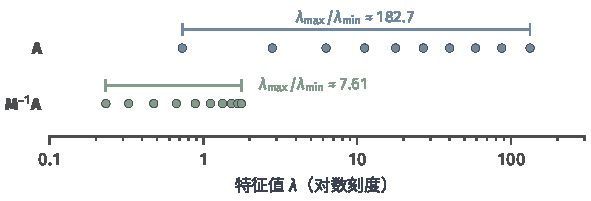
\includegraphics[width=100mm]{figures/01-basic-mathematics/03-vectors-matrices-and-multivariate-functions/matplotlib/c5-preconditioned-spectrum/figure.pdf}
  \caption{对角缩放前后的特征值分布（对数横轴）。矩阵为$\bm A=\bm S\bm T\bm S$，$\bm S=\operatorname{diag}(1,\ldots,10)$，$\bm T$为对角元$1$、次对角元$0.4$的三对角矩阵，预条件$\bm M=\operatorname{diag}(\bm A)$。蓝点为$\bm A$的$10$个特征值（数值计算），绿点为$\bm M^{-1}\bm A$的特征值$1+0.8\cos(j\pi/11)$；括线标出各自的范围与最大、最小特征值之比。}
  \label{fig:ls-preconditioned-spectrum}
\end{figure}

\subsubsection{SSOR预条件}

\paragraph{构造}
对角预条件丢掉了$\bm A$的全部非对角元。要保留更多信息，可以借用第~\ref{sec:ls-ssor}节的SSOR迭代。把对称矩阵写成
\[
 \bm A=\bm D+\bm L+\bm L^\top ,
\]
其中$\bm D$是对角部分，$\bm L$是严格下三角部分。SSOR迭代每一轮先作一次前向扫掠、再作一次反向扫掠，把残差$\bm r_k$变成修正量$\bm\delta_k$（式~\eqref{eq:ls-ssor-correction}）。这一修正是$\bm r_k$的线性函数，记作$\bm\delta_k=\bm M^{-1}\bm r_k$，其中
\begin{equation}
 \bm M=\frac{1}{\omega(2-\omega)}(\bm D+\omega\bm L)\bm D^{-1}(\bm D+\omega\bm L)^\top,\qquad 0<\omega<2 .
 \label{eq:ls-ssor-preconditioner-matrix}
\end{equation}
这个$\bm M$就是SSOR预条件。取$\omega=1$时展开可得
\begin{equation}
 \bm M=(\bm D+\bm L)\bm D^{-1}(\bm D+\bm L^\top)=\bm A+\bm L\bm D^{-1}\bm L^\top ,
 \label{eq:ls-ssor-preconditioner-difference}
\end{equation}
即$\bm M$与$\bm A$只差一项$\bm L\bm D^{-1}\bm L^\top$。

求解$\bm M\bm z=\bm r$不需要形成$\bm M$。记$\bm F=\bm D+\omega\bm L$，它是下三角矩阵，于是$\bm M\bm z=\bm r$可以拆成三步：先解下三角方程，再作对角缩放，最后解上三角方程，
\begin{equation}
 \bm F\bm y=\bm r,\qquad \bm t=\omega(2-\omega)\bm D\bm y,\qquad \bm F^\top\bm z=\bm t .
 \label{eq:ls-ssor-preconditioner}
\end{equation}
三步依次给出$\bm y=\bm F^{-1}\bm r$与$\bm z=\bm F^{-\top}\bm t$，合起来正是
\[
 \bm z=\omega(2-\omega)\bm F^{-\top}\bm D\bm F^{-1}\bm r=\bm M^{-1}\bm r .
\]

例中取$\omega=1$，严格下三角部分与修正项为
\[
 \bm L=\begin{bmatrix}0&0\\1&0\end{bmatrix},\qquad
 \bm L\bm D^{-1}\bm L^\top=\begin{bmatrix}0&0\\0&1/4\end{bmatrix},
\]
所以
\[
 \bm M=\begin{bmatrix}4&1\\1&13/4\end{bmatrix},
\]
它与$\bm A$只在右下角差$1/4$，比对角预条件接近得多。

对$\bm r=(1,2)^\top$求解一次。前代、缩放与回代依次得到
\[
 \bm y=\begin{bmatrix}1/4\\7/12\end{bmatrix},\qquad
 \bm t=\bm D\bm y=\begin{bmatrix}1\\7/4\end{bmatrix},\qquad
 \bm z=\begin{bmatrix}5/48\\7/12\end{bmatrix}.
\]
这正是第~\ref{sec:ls-ssor}节从零初值作一轮SSOR迭代得到的$\bm x_1$。

\paragraph{性质}
SSOR预条件保留了$\bm A$的全部元素，只多出一项$\bm L\bm D^{-1}\bm L^\top$（$\omega=1$时），通常比对角预条件更接近$\bm A$。$\bm A$对称正定且$0<\omega<2$时，$\bm M$也对称正定。它不需要额外存储：所用的三角矩阵$\bm F$就是$\bm A$的下三角部分。每次求解相当于两次三角扫掠，代价约为两次矩阵乘向量；扫掠必须按分量顺序进行，难以并行。$\omega$一经选定，在整个求解过程中就不再改变。

\paragraph{应用场景}
SSOR预条件适合中等规模的对称正定稀疏矩阵，例如椭圆型偏微分方程的离散化：它几乎不需要构造代价，效果又比对角预条件好。预条件的效果对$\omega$不如SSOR迭代本身那样敏感，通常取$\omega=1$，即对称Gauss--Seidel预条件，就已够用。

\subsubsection{不完全分解}

\paragraph{为什么要不完全}
最接近$\bm A$的选择是$\bm A$自己的分解：若$\bm A=\bm L\bm U$，取$\bm M=\bm L\bm U$就有$\bm M=\bm A$，一步即可结束。问题在于，即使$\bm A$很稀疏，它的三角因子也往往稠密得多。消元时，第$i$行减去第$k$行的倍数，会在第$i$行原来为零、而第$k$行不为零的位置上产生新的非零元，称为\term{填充}（fill-in）。填充使存储和三角求解的代价都大大增加。

作为预条件，并不需要精确的因子，只需要$\bm M$接近$\bm A$、三角求解便宜。\term{不完全分解}（incomplete factorization）的做法是：照常执行第~\ref{chap:direct-linear-solvers}章的消元，但事先规定因子允许出现非零元的位置集合$\mathcal S$，消元中凡是落在$\mathcal S$之外的填充一律舍去。最常用的$\mathcal S$就是$\bm A$自身非零元的位置（总含全部对角位置），这时因子与$\bm A$一样稀疏。

\paragraph{不完全LU分解}
回忆第~\ref{sec:ls-lu}节不选主元的LU消元：对$k=1,\ldots,d-1$，用第$k$行消去其下各行的第$k$列元素，
\[
 l_{i,k}=\frac{w_{i,k}}{w_{k,k}},\qquad
 w_{i,j}\leftarrow w_{i,j}-l_{i,k}w_{k,j}\quad(i,j>k),
\]
其中$\bm W$从$\bm A$开始，消元结束时成为$\bm U$。

不完全LU只改动一处：乘子$l_{i,k}$只在$(i,k)\in\mathcal S$时计算，尾块更新只在$(i,j)\in\mathcal S$时执行，其余位置保持为零，相当于把那里产生的填充直接丢掉。为了不破坏规定的稀疏模式，通常不选主元。

结束时得到单位下三角矩阵$\widetilde{\bm L}$与上三角矩阵$\widetilde{\bm U}$，它们的非零元都在$\mathcal S$中，预条件取为
\begin{equation}
 \bm M=\widetilde{\bm L}\widetilde{\bm U} .
 \label{eq:ls-ilu-preconditioner}
\end{equation}
求解$\bm M\bm z=\bm r$就是先解$\widetilde{\bm L}\bm y=\bm r$，再解$\widetilde{\bm U}\bm z=\bm y$，即第~\ref{sec:ls-lu}节的前代~\eqref{eq:ls-forward-substitution}与回代~\eqref{eq:ls-back-substitution}，只是两个因子都是稀疏的。$\bm M$与$\bm A$的差别恰好来自被舍去的填充：若在完整消元中保留它们，所得因子之积就是$\bm A$。

\paragraph{不完全Cholesky分解}
$\bm A$对称正定时，用第~\ref{sec:ls-cholesky}节的Cholesky分解代替LU，得到\term{不完全Cholesky分解}（incomplete Cholesky factorization）。做法相同：按列公式~\eqref{eq:ls-cholesky-columns}逐列计算，但只计算位于$\mathcal S$中的元素，$\mathcal S$之外的元素直接取零。对$j=1,\ldots,d$，
\begin{equation}
 \begin{gathered}
 l_{j,j}=\sqrt{a_{j,j}-\sum_{k<j}l_{j,k}^2},\\
 l_{i,j}=\begin{cases}\dfrac{a_{i,j}-\sum_{k<j}l_{i,k}l_{j,k}}{l_{j,j}},&(i,j)\in\mathcal S,\\[1ex] 0,&(i,j)\notin\mathcal S,\end{cases}\qquad(i>j).
 \end{gathered}
 \label{eq:ls-incomplete-cholesky}
\end{equation}
结束时得到稀疏的下三角矩阵$\bm L$，预条件取为
\begin{equation}
 \bm M=\bm L\bm L^\top ,
 \label{eq:ls-ic-preconditioner}
\end{equation}
求解$\bm M\bm z=\bm r$同样是一次前代与一次回代。不完全Cholesky就是对称情形下的不完全LU：两者舍去的是同样位置上的填充，$\bm L$与$\widetilde{\bm L}$只差各列的一个正的缩放因子。

\paragraph{例子}
二阶的例子没有填充可舍，下面换用
\[
 \bm A=\begin{bmatrix}4&1&1\\1&4&0\\1&0&4\end{bmatrix},
\]
它的$(2,3)$与$(3,2)$元为零，取$\mathcal S$为$\bm A$的非零位置。

先看完整的LU消元。第一步乘子为$l_{2,1}=l_{3,1}=1/4$，第二、三行减去第一行的$1/4$后，
\[
 \bm W=\begin{bmatrix}4&1&1\\0&15/4&-1/4\\0&-1/4&15/4\end{bmatrix}.
\]
原来为零的$(2,3)$与$(3,2)$位置出现了$-1/4$，这就是填充；第二步还要用它算出$l_{3,2}=-1/15$。

不完全LU把这两个填充舍去，第一步后得到
\[
 \bm W=\begin{bmatrix}4&1&1\\0&15/4&0\\0&0&15/4\end{bmatrix},
\]
第二步的乘子$l_{3,2}$不在$\mathcal S$中，取零。于是
\[
 \begin{gathered}
 \widetilde{\bm L}=\begin{bmatrix}1&0&0\\1/4&1&0\\1/4&0&1\end{bmatrix},\\
 \widetilde{\bm U}=\begin{bmatrix}4&1&1\\0&15/4&0\\0&0&15/4\end{bmatrix},
 \end{gathered}
\]
预条件为
\[
 \bm M=\widetilde{\bm L}\widetilde{\bm U}=\begin{bmatrix}4&1&1\\1&4&1/4\\1&1/4&4\end{bmatrix}.
\]
$\bm M$与$\bm A$只在$(2,3)$、$(3,2)$两处不同，差值$1/4$正是被舍去的填充$-1/4$的相反数；两个因子与$\bm A$一样稀疏。

按式~\eqref{eq:ls-incomplete-cholesky}作不完全Cholesky，得
\[
 \bm L=\begin{bmatrix}2&0&0\\1/2&\sqrt{15}/2&0\\1/2&0&\sqrt{15}/2\end{bmatrix},
\]
它的各列是$\widetilde{\bm L}$的各列分别乘以$2,\sqrt{15}/2,\sqrt{15}/2$，所以$\bm L\bm L^\top$给出同一个$\bm M$。

\paragraph{性质}
不完全分解的$\bm M$与$\bm A$的差就是被舍去的填充所产生的影响。$\mathcal S$取得越大，舍去的越少，$\bm M$越接近$\bm A$，效果越好，但因子越稠密，构造与求解的代价也越高；$\mathcal S$取$\bm A$的非零位置是最常见的折中。

不完全分解可能失败。完整Cholesky分解在$\bm A$对称正定时，每一列开方前的量都为正；舍去填充之后，这一保证就不再成立，开方前的量可能为零或为负。所以构造时必须逐列检查，出现非正值时报告失败，或给对角元加上一个正的移位后重新构造。不完全LU也可能遇到零主元。

构造成功时，不完全Cholesky给出的$\bm M$对称正定；不完全LU给出的$\bm M$一般不对称。

\paragraph{应用场景}
不完全分解是一般稀疏矩阵最常用的预条件之一。对称正定矩阵用不完全Cholesky，非对称矩阵用不完全LU。它需要先付出构造代价并存储因子，所以适合条件很差、对角与SSOR预条件不足以显著减少步数的问题，或者需要用同一个矩阵求解多个右端的情形。

\subsection{预条件的使用}
\label{sec:ls-preconditioner-usage}

有了$\bm M$，还要决定$\bm M^{-1}$放在哪里。前面左乘$\bm M^{-1}$只是一种选择，称为左预条件；也可以把$\bm M^{-1}$乘在$\bm A$的右边，称为右预条件：
\begin{equation}
 \bm M^{-1}\bm A\bm x=\bm M^{-1}\bm b,\qquad
 \bm A\bm M^{-1}\bm y=\bm b,\quad \bm x=\bm M^{-1}\bm y .
 \label{eq:ls-left-right-preconditioning}
\end{equation}
由$\bm A\bm M^{-1}=\bm M(\bm M^{-1}\bm A)\bm M^{-1}$，两个矩阵相似，特征值相同，所以从谱的角度看，两种做法加速的效果一样。它们的区别在于求解器看到的残差和未知量是什么，这决定了停止判断是否可靠、最小二乘的目标是否保持。

此外，CG只适用于对称正定矩阵，而$\bm M^{-1}\bm A$与$\bm A\bm M^{-1}$一般都不对称，所以CG需要第三种用法。下面依次讨论这三种用法，每种各取一个求解器，写出带预条件后的计算过程。

\subsubsection{左预条件}

\paragraph{思想}
左预条件求解式~\eqref{eq:ls-left-right-preconditioning}的第一式。未知量仍是$\bm x$，求解器把$\bm M^{-1}\bm A$当作系数矩阵、把$\bm M^{-1}\bm b$当作右端，算法本身一字不改。唯一的变化是：每当求解器需要系数矩阵乘向量$\bm v$时，先算$\bm A\bm v$，再解一次$\bm M\bm w=\bm A\bm v$。这种方式简单直接，GMRES与BiCGSTAB常用它。

它的缺点是改变了残差。求解器算出的残差是
\begin{equation}
 \tilde{\bm r}=\bm M^{-1}\bm b-\bm M^{-1}\bm A\bm x=\bm M^{-1}\bm r ,
 \label{eq:ls-left-preconditioned-residual}
\end{equation}
而不是原方程的残差$\bm r=\bm b-\bm A\bm x$。GMRES最小化的是$\lVert\bm M^{-1}\bm r\rVert_2$，按递推估计停止时，阈值检查的也是这个量；它与$\lVert\bm r\rVert_2$可以相差很多，最多可差$\bm M$的条件数倍。所以停止前必须用$\bm b-\bm A\bm x$重新计算原残差并复核。

对不相容的最小二乘问题，改变残差就改变了目标：
\[
 \lVert\bm M^{-1}(\bm b-\bm A\bm x)\rVert_2^2=(\bm b-\bm A\bm x)^\top\bm M^{-\top}\bm M^{-1}(\bm b-\bm A\bm x)
\]
是第~\ref{sec:ls-weighted-ls}节以$\bm M^{-\top}\bm M^{-1}$为权的加权最小二乘，一般会得到不同的解。所以最小二乘求解器不用左预条件。

MINRES也属于这一类，但它要求系数矩阵对称，而$\bm M^{-1}\bm A$不对称。它的预条件版本取对称正定的$\bm M$，把通常的内积换成$\bm M$诱导的内积，最小化的是$(\bm r^\top\bm M^{-1}\bm r)^{1/2}$，同样不是原残差的长度。

\paragraph{计算过程：左预条件GMRES}
与第~\ref{sec:ls-gmres}节相比，只有两处改动：初始残差换成预条件残差，Arnoldi扩展中的矩阵乘向量后接一次辅助求解。每一步使用例~\ref{ex:ls-stationary-running-example}的数据进行演示：
\[
 \bm A=\begin{bmatrix}4&1\\1&3\end{bmatrix},\qquad
 \bm b=\begin{bmatrix}1\\2\end{bmatrix},\qquad
 \bm x_0=\bm 0 .
\]
取对角预条件$\bm M=\operatorname{diag}(4,3)$，于是
\[
 \widetilde{\bm A}=\bm M^{-1}\bm A=\begin{bmatrix}1&1/4\\1/3&1\end{bmatrix}.
\]

\paragraph{变量}
\begin{itemize}
 \item 第~\ref{sec:ls-gmres}节的全部变量：周期起点$\bm x^{(s)}$、基$\bm v_1,\ldots,\bm v_{j+1}$、工作向量$\bm w$、$\overline{\bm H}_j$的各列、旋转$c_i,s_i$与右端$\bm g$；其中$\bm v_i$是$\mathcal K_j(\widetilde{\bm A},\tilde{\bm r}_0)$的基，$\lvert g_{j+1}\rvert$估计的是预条件残差的长度。
 \item 预条件$\bm M$：只用于求解$\bm M\bm z=\bm r$。
\end{itemize}

\paragraph{初始化}
把预条件残差初始化为$\tilde{\bm r}_0=\bm M^{-1}(\bm b-\bm A\bm x_0)$，其余与GMRES相同：
\[
 \beta=\lVert\tilde{\bm r}_0\rVert_2,\qquad \bm v_1=\frac{\tilde{\bm r}_0}{\beta},\qquad g_1=\beta,\qquad j=1 .
\]
例中$\tilde{\bm r}_0=(1/4,2/3)^\top$，
\[
 \beta=\frac{\sqrt{73}}{12}\approx0.7120,\qquad \bm v_1=\frac1{\sqrt{73}}\begin{bmatrix}3\\8\end{bmatrix}.
\]

\paragraph{每轮更新}
在第$j$轮：
\begin{enumerate}
 \item \textbf{乘矩阵并作辅助求解。}计算$\bm A\bm v_j$，再解
 \[
  \bm M\bm w=\bm A\bm v_j ,
 \]
 得到$\bm w=\widetilde{\bm A}\bm v_j$。例中第一轮$\bm A\bm v_1=(20,27)^\top/\sqrt{73}$，逐分量相除得
 \[
  \bm w=\frac1{\sqrt{73}}\begin{bmatrix}5\\9\end{bmatrix}.
 \]

 \item \textbf{Arnoldi正交化。}对$\bm w$按第~\ref{sec:ls-arnoldi}节的式~\eqref{eq:ls-arnoldi-coefficients}与\eqref{eq:ls-arnoldi-normalize}正交化并归一化，得到$\overline{\bm H}_j$的第$j$列与$\bm v_{j+1}$。例中第一轮
 \[
  h_{1,1}=\frac{87}{73},\qquad h_{2,1}=\frac{13}{73},\qquad \bm v_2=\frac1{\sqrt{73}}\begin{bmatrix}8\\-3\end{bmatrix}.
 \]

 \item \textbf{旋转与右端。}按第~\ref{sec:ls-gmres}节每轮更新的第2—4步，对新列作用旧旋转、构造新旋转，并按式~\eqref{eq:ls-gmres-rhs}更新右端。例中第一轮
 \[
  \rho_1=\frac{\sqrt{7738}}{73}\approx1.2050,\qquad
  \lvert g_2\rvert=\frac{\beta h_{2,1}}{\rho_1}=\frac{13}{12\sqrt{106}}\approx0.1052 .
 \]
 若此时回代，得
 \[
  \bm x_1=\begin{bmatrix}87/424\\29/53\end{bmatrix}\approx\begin{bmatrix}0.2052\\0.5472\end{bmatrix},
 \]
 它的原残差
 \[
  \bm r_1=\bm b-\bm A\bm x_1=\begin{bmatrix}-39/106\\65/424\end{bmatrix},\qquad \lVert\bm r_1\rVert_2\approx0.3986,
 \]
 而$\lVert\bm M^{-1}\bm r_1\rVert_2\approx0.1052$恰为$\lvert g_2\rvert$：GMRES报告的残差比原残差小了将近$4$倍。

 例中第二轮由第1步，
 \[
  \bm A\bm v_2=\frac1{\sqrt{73}}\begin{bmatrix}29\\-1\end{bmatrix},\qquad
  \bm w=\frac1{\sqrt{73}}\begin{bmatrix}29/4\\-1/3\end{bmatrix};
 \]
 由第2步，
 \[
  h_{1,2}=\frac{229}{876},\qquad h_{2,2}=\frac{59}{73},\qquad h_{3,2}=0 ,
 \]
 于是$g_3=0$。

 \item \textbf{停止。}若$\lvert g_{j+1}\rvert\le\tau$、$h_{j+1,j}=0$或已达到步数上限，退出每轮更新，按GMRES回代并还原$\bm x$；由于$\lvert g_{j+1}\rvert$度量的是预条件残差，退出后必须用$\bm b-\bm A\bm x$复核原残差，按第~\ref{sec:ls-stationary-stopping}节判断是否达到容差。

 例中第二轮$h_{3,2}=0$，退出迭代。
\end{enumerate}

最终回代得
\[
 \bm x_2=\bm x_\star=\begin{bmatrix}1/11\\7/11\end{bmatrix},
\]
复核原残差为零。与无预条件的GMRES相比，两者都两步结束；第一步的原残差由$0.542$降到$0.399$，但停止判断所用的估计$0.105$与原残差并不相等，这就是左预条件对残差的扭曲。

\subsubsection{右预条件}

\paragraph{思想}
右预条件求解式~\eqref{eq:ls-left-right-preconditioning}的第二式。求解器把$\bm A\bm M^{-1}$当作系数矩阵，未知量换成$\bm y=\bm M\bm x$。每当需要系数矩阵乘向量$\bm v$时，先解一次$\bm M\bm z=\bm v$，再算$\bm A\bm z$。

这样做的好处是残差不变。对任意$\bm y$，记$\bm x=\bm M^{-1}\bm y$，有
\begin{equation}
 \bm b-\bm A\bm M^{-1}\bm y=\bm b-\bm A\bm x ,
 \label{eq:ls-right-preconditioned-residual}
\end{equation}
所以求解器算出的残差就是原方程的真实残差。GMRES这类最小残差方法最小化的正是$\lVert\bm b-\bm A\bm x\rVert_2$，递推估计与停止阈值都直接针对它；对最小二乘问题，目标$\lVert\bm b-\bm A\bm x\rVert_2$与解集也都保持不变。

右预条件的另一个特点是变量解耦。整个迭代只在$\bm y$上进行，$\bm M$只出现在系数矩阵的作用里，不进入解的递推；原变量$\bm x$只在结束时由一次求解$\bm M\bm x=\bm y$得到。

因此，LSQR与LSMR采用右预条件；GMRES需要直接控制原残差时也常用它。LSQR与LSMR还要用到系数矩阵的转置乘向量，这时$(\bm A\bm M^{-1})^\top\bm u=\bm M^{-\top}(\bm A^\top\bm u)$，即先乘$\bm A^\top$，再解一次$\bm M^\top\bm z=\bm A^\top\bm u$。

有两点需要注意。

其一，LSQR报告的正规残差估计变成了$\lVert\bm M^{-\top}\bm A^\top\bm r\rVert_2$，不再是$\lVert\bm A^\top\bm r\rVert_2$。

其二，零初值下LSQR选出的是$\lVert\bm y\rVert_2=\lVert\bm M\bm x\rVert_2$最小的最小二乘解；$\bm A$秩亏时，它未必是原坐标下欧氏范数最小的那个解。

\paragraph{计算过程：右预条件LSQR}
与第~\ref{sec:ls-lsqr}节相比，双对角化中的两次矩阵作用各接一次辅助求解，解的累加改在$\bm y$上进行，结束时换回$\bm x$。每一步使用第~\ref{sec:ls-lsqr}节的不相容系统进行演示：
\[
 \bm A=\begin{bmatrix}1&0\\0&2\\0&0\end{bmatrix},\qquad
 \bm b=\begin{bmatrix}1\\1\\1\end{bmatrix},
\]
取列缩放$\bm M=\operatorname{diag}(\lVert\bm a_1\rVert_2,\lVert\bm a_2\rVert_2)=\operatorname{diag}(1,2)$，于是
\[
 \widehat{\bm A}=\bm A\bm M^{-1}=\begin{bmatrix}1&0\\0&1\\0&0\end{bmatrix}
\]
的两列已是标准正交的。

\paragraph{变量}
\begin{itemize}
 \item 第~\ref{sec:ls-lsqr}节的全部变量：基向量$\bm u,\bm v$，双对角系数$\alpha,\beta$，正交变换的$\rho,\bar\rho,c,s,\theta,\phi,\bar\phi$与方向$\bm w$；它们都针对$\widehat{\bm A}$。
 \item $\bm y\in\mathbb R^d$：$\bm y$坐标下的近似解，代替LSQR中的$\bm x$累加。
 \item 预条件$\bm M$：用于求解$\bm M\bm z=\bm v$与$\bm M^\top\bm z=\bm A^\top\bm u$。
\end{itemize}

\paragraph{初始化}
按式~\eqref{eq:ls-golub-kahan-start}起步，其中$\widehat{\bm A}^\top\bm u_1=\bm M^{-\top}(\bm A^\top\bm u_1)$；把$\bm y$初始化为零，其余与LSQR相同：
\[
 \bm y_0=\bm 0,\qquad \bm w_1=\bm v_1,\qquad \bar\rho_1=\alpha_1,\qquad \bar\phi_1=\beta_1 .
\]
例中$\beta_1=\sqrt3$，$\bm u_1=(1,1,1)^\top/\sqrt3$。先乘$\bm A^\top$，再作辅助求解，得
\[
 \bm A^\top\bm u_1=\frac1{\sqrt3}\begin{bmatrix}1\\2\end{bmatrix},\qquad
 \widehat{\bm A}^\top\bm u_1=\bm M^{-\top}(\bm A^\top\bm u_1)=\frac1{\sqrt3}\begin{bmatrix}1\\1\end{bmatrix},
\]
故
\[
 \alpha_1=\sqrt{\frac23},\qquad \bm v_1=\frac1{\sqrt2}\begin{bmatrix}1\\1\end{bmatrix}.
\]

\paragraph{每轮更新}
在第$k$轮：
\begin{enumerate}
 \item \textbf{带辅助求解的双对角化。}按式~\eqref{eq:ls-golub-kahan-step}扩展一步，其中
 \begin{equation}
  \widehat{\bm A}\bm v_k=\bm A(\bm M^{-1}\bm v_k),\qquad \widehat{\bm A}^\top\bm u_{k+1}=\bm M^{-\top}(\bm A^\top\bm u_{k+1}).
  \label{eq:ls-preconditioned-lsqr-products}
 \end{equation}
 例中第一轮先作辅助求解，再乘$\bm A$，
 \[
  \bm M^{-1}\bm v_1=\frac1{\sqrt2}\begin{bmatrix}1\\1/2\end{bmatrix},\qquad
  \widehat{\bm A}\bm v_1=\frac1{\sqrt2}\begin{bmatrix}1\\1\\0\end{bmatrix},
 \]
 扣除$\alpha_1\bm u_1$后
 \[
  \beta_2=\frac1{\sqrt3},\qquad \bm u_2=\frac1{\sqrt6}\begin{bmatrix}1\\1\\-2\end{bmatrix};
 \]
 $\widehat{\bm A}^\top\bm u_2=(1,1)^\top/\sqrt6$恰好等于$\beta_2\bm v_1$，所以$\alpha_2=0$。

 \item \textbf{正交变换。}按式~\eqref{eq:ls-lsqr-rotation}消去$\beta_{k+1}$。例中第一轮
 \[
  \begin{gathered}
  \rho_1=1,\qquad c_1=\sqrt{\frac23},\qquad s_1=\frac1{\sqrt3},\\
  \theta_2=0,\qquad \phi_1=\sqrt2,\qquad \bar\phi_2=1 .
  \end{gathered}
 \]

 \item \textbf{在$\bm y$坐标中更新解与方向。}按式~\eqref{eq:ls-lsqr-update}与\eqref{eq:ls-lsqr-direction}，把其中的$\bm x$换成$\bm y$：
 \[
  \bm y_k=\bm y_{k-1}+\frac{\phi_k}{\rho_k}\bm w_k,\qquad \bm w_{k+1}=\bm v_{k+1}-\frac{\theta_{k+1}}{\rho_k}\bm w_k .
 \]
 例中第一轮
 \[
  \bm y_1=\sqrt2\,\bm w_1=\begin{bmatrix}1\\1\end{bmatrix}.
 \]

 \item \textbf{停止。}按式~\eqref{eq:ls-lsqr-estimates}读出两个估计：$\lvert\bar\phi_{k+1}\rvert$就是原残差的长度，另一个是$\lVert\bm M^{-\top}\bm A^\top\bm r_k\rVert_2$。达到阈值、出现零系数或步数用尽时退出，换回$\bm x_k=\bm M^{-1}\bm y_k$并复核真实残差。

 例中第一轮原残差估计为$1$，正规残差估计为$\lvert\bar\phi_2\rvert\alpha_2\lvert c_1\rvert=0$，且$\alpha_2=0$，退出迭代。
\end{enumerate}

最终换回原变量
\[
 \bm x_1=\bm M^{-1}\bm y_1=\begin{bmatrix}1\\1/2\end{bmatrix}=\hat{\bm x},
\]
真实残差为$(0,0,1)^\top$，长度恰为估计值$1$：右预条件下递推看到的就是原残差。

无预条件的LSQR在这个例子上需要两轮（第~\ref{sec:ls-lsqr}节）；列缩放使$\widehat{\bm A}$的列标准正交，一轮即得最小二乘解。

\subsubsection{预条件共轭梯度法}
\label{sec:ls-pcg}

\paragraph{CG对$\bm M$的要求}
CG要求系数矩阵对称正定，左、右预条件都不满足这一点：即使$\bm A$与$\bm M$都对称正定，$\bm M^{-1}\bm A$与$\bm A\bm M^{-1}$一般也不对称。左预条件GMRES的例子中
\[
 \bm M^{-1}\bm A=\begin{bmatrix}1&1/4\\1/3&1\end{bmatrix}
\]
就不对称。对这样的矩阵，CG的残差正交与方向共轭都不再成立。

所以用于CG的预条件需要另作处理。

首先，$\bm M$本身必须对称正定，并在整个迭代中固定不变；对角预条件、SSOR预条件以及构造成功的不完全Cholesky都满足这一点，不完全LU则一般不满足。

其次，$\bm M^{-1}$不能只乘在一侧，而要把$\bm M$拆成两个互为转置的因子，分别乘在$\bm A$的两侧，使变换后的矩阵仍然对称正定。

\paragraph{保持对称的变换}
设$\bm A$与$\bm M$都对称正定，写$\bm M=\bm C\bm C^\top$，代换$\bm x=\bm C^{-\top}\bm y$并左乘$\bm C^{-1}$，得到
\begin{equation}
 \widehat{\bm A}\bm y=\bm C^{-1}\bm b,\qquad \widehat{\bm A}=\bm C^{-1}\bm A\bm C^{-\top},
 \label{eq:ls-pcg-transformed-system}
\end{equation}
其中$\widehat{\bm A}$对称正定：对$\bm w\neq\bm0$有
\[
 \bm w^\top\widehat{\bm A}\bm w=(\bm C^{-\top}\bm w)^\top\bm A(\bm C^{-\top}\bm w)>0 ,
\]
可以施行CG。$\widehat{\bm A}=\bm C^\top(\bm M^{-1}\bm A)\bm C^{-\top}$与$\bm M^{-1}\bm A$相似，所以改善的正是$\bm M^{-1}\bm A$的谱。

\paragraph{递推}
对式~\eqref{eq:ls-pcg-transformed-system}施行CG再换回原变量（定理~\ref{thm:ls-pcg-equivalence}），$\bm C$从公式中消失，得到\term{预条件共轭梯度法}（preconditioned conjugate gradient method，PCG）。记预条件残差$\bm z_k=\bm M^{-1}\bm r_k$与配对量$\tau_k=\bm r_k^\top\bm z_k$，步长与组合系数为
\begin{equation}
 \alpha_k=\frac{\tau_k}{\bm p_k^\top\bm A\bm p_k},\qquad \beta_k=\frac{\tau_{k+1}}{\tau_k},
 \label{eq:ls-pcg-coefficients}
\end{equation}
解、残差与方向按
\begin{equation}
 \begin{gathered}
 \bm x_{k+1}=\bm x_k+\alpha_k\bm p_k,\qquad
 \bm r_{k+1}=\bm r_k-\alpha_k\bm A\bm p_k,\\
 \bm p_0=\bm z_0,\qquad \bm p_{k+1}=\bm z_{k+1}+\beta_k\bm p_k
 \end{gathered}
 \label{eq:ls-pcg-updates}
\end{equation}
更新。与CG的式~\eqref{eq:ls-cg-update}—\eqref{eq:ls-cg-beta}相比，只是新方向由$\bm z$而不是$\bm r$组合而成，内积$\bm r^\top\bm r$换成$\bm r^\top\bm z$；递推中的残差仍是原残差，停止判断不受扭曲。每轮比CG多一次辅助求解$\bm M\bm z_{k+1}=\bm r_{k+1}$。

\begin{theorem}[PCG与变换后CG的等价]
\label{thm:ls-pcg-equivalence}
设$\bm A,\bm M$对称正定，$\bm M=\bm C\bm C^\top$，$\widehat{\bm A}=\bm C^{-1}\bm A\bm C^{-\top}$。在精确算术中，只要PCG尚未终止，它的迭代量与对$\widehat{\bm A}\bm y=\bm C^{-1}\bm b$从$\bm y_0=\bm C^\top\bm x_0$施行CG所得的迭代量满足
\begin{equation}
 \bm y_k=\bm C^\top\bm x_k,\qquad \hat{\bm r}_k=\bm C^{-1}\bm r_k,\qquad \hat{\bm p}_k=\bm C^\top\bm p_k .
 \label{eq:ls-pcg-correspondence}
\end{equation}
因此$\bm x_k$是$\bm x_0+\mathcal K_k(\bm M^{-1}\bm A,\bm M^{-1}\bm r_0)$中使$\lVert\bm x-\bm x_\star\rVert_{\bm A}$最小的唯一点，并且
\begin{equation}
 \begin{gathered}
 \lVert\bm x_k-\bm x_\star\rVert_{\bm A}\le2\Bigl(\frac{\sqrt{\hat\kappa}-1}{\sqrt{\hat\kappa}+1}\Bigr)^k\lVert\bm x_0-\bm x_\star\rVert_{\bm A},\\
 \hat\kappa=\kappa_2(\widehat{\bm A})=\frac{\lambda_{\max}(\bm M^{-1}\bm A)}{\lambda_{\min}(\bm M^{-1}\bm A)} .
 \end{gathered}
 \label{eq:ls-pcg-convergence-bound}
\end{equation}
\end{theorem}

\begin{proof}
先对$k$归纳证明迭代量的对应关系，再把CG的最优性与收敛界换回原变量。

\emph{起点。}由$\widehat{\bm A}$的定义，
\[
 \hat{\bm r}_0=\bm C^{-1}\bm b-\widehat{\bm A}\bm C^\top\bm x_0=\bm C^{-1}\bm r_0 ,
\]
而$\bm C^{-\top}\bm C^{-1}=\bm M^{-1}$，故
\[
 \hat{\bm p}_0=\hat{\bm r}_0=\bm C^\top(\bm M^{-1}\bm r_0)=\bm C^\top\bm z_0=\bm C^\top\bm p_0 .
\]

\emph{系数相同。}设第$k$步对应关系成立。CG步长中的两个内积逐项换算为
\[
 \begin{aligned}
 \hat{\bm r}_k^\top\hat{\bm r}_k&=\bm r_k^\top\bm M^{-1}\bm r_k=\tau_k,\\
 \hat{\bm p}_k^\top\widehat{\bm A}\hat{\bm p}_k&=\bm p_k^\top\bm C\bigl(\bm C^{-1}\bm A\bm C^{-\top}\bigr)\bm C^\top\bm p_k=\bm p_k^\top\bm A\bm p_k ,
 \end{aligned}
\]
所以CG的步长等于式~\eqref{eq:ls-pcg-coefficients}的$\alpha_k$；同理组合系数同为$\tau_{k+1}/\tau_k$。

\emph{迭代量对应。}系数相同，于是
\[
 \bm y_{k+1}=\bm C^\top(\bm x_k+\alpha_k\bm p_k)=\bm C^\top\bm x_{k+1} .
\]
再由$\widehat{\bm A}\hat{\bm p}_k=\bm C^{-1}\bm A\bm p_k$得
\[
 \begin{aligned}
 \hat{\bm r}_{k+1}&=\bm C^{-1}(\bm r_k-\alpha_k\bm A\bm p_k)=\bm C^{-1}\bm r_{k+1},\\
 \hat{\bm p}_{k+1}&=\bm C^{-1}\bm r_{k+1}+\beta_k\bm C^\top\bm p_k\\
 &=\bm C^\top(\bm z_{k+1}+\beta_k\bm p_k)=\bm C^\top\bm p_{k+1}.
 \end{aligned}
\]

\emph{最优性与收敛界。}由定理~\ref{thm:ls-cg-convergence}，$\bm y_k$是$\bm y_0+\mathcal K_k(\widehat{\bm A},\hat{\bm r}_0)$中使$\lVert\bm y-\bm C^\top\bm x_\star\rVert_{\widehat{\bm A}}$最小的唯一点。换回$\bm x=\bm C^{-\top}\bm y$时，
\[
 \begin{gathered}
 \lVert\bm C^\top(\bm x-\bm x_\star)\rVert_{\widehat{\bm A}}=\lVert\bm x-\bm x_\star\rVert_{\bm A},\\
 \bm C^{-\top}\widehat{\bm A}^j\hat{\bm r}_0=(\bm M^{-1}\bm A)^j\bm M^{-1}\bm r_0 ,
 \end{gathered}
\]
所以仿射子空间和目标都对应过来，收敛界也随之成立。最后，$\bm M^{-1}\bm A=\bm C^{-\top}\widehat{\bm A}\bm C^\top$与$\widehat{\bm A}$相似，而$\widehat{\bm A}$对称正定，$\kappa_2(\widehat{\bm A})$就是特征值之比。
\end{proof}

定理中的$\bm C$只用于论证，算法只需求解$\bm M\bm z=\bm r$；收敛速度由$\bm M^{-1}\bm A$的特征值之比$\hat\kappa$决定，图~\ref{fig:ls-preconditioned-spectrum}中对角缩放把它从约$182.7$降到约$7.61$。论证要求整个迭代使用同一个固定的线性作用$\bm M^{-1}$；预条件随轮次变化时，标准PCG的共轭性与最优性不再沿用。

\paragraph{计算过程}
下面写出PCG的计算过程。每一步使用例~\ref{ex:ls-stationary-running-example}的数据进行演示：
\[
 \bm A=\begin{bmatrix}4&1\\1&3\end{bmatrix},\qquad
 \bm b=\begin{bmatrix}1\\2\end{bmatrix},\qquad
 \bm x_0=\bm0 .
\]
精确解为$\bm x_\star=(1/11,7/11)^\top$。预条件取对角预条件$\bm M=\operatorname{diag}(4,3)$，它对称正定，满足上面的要求。

预先选定的参数为$\mathrm{atol},\mathrm{rtol},K$；停止检查沿用第~\ref{sec:ls-stationary-stopping}节，按原残差判断。这里的$\alpha_k,\beta_k$是CG的步长与组合系数，与双对角化的系数无关。

\paragraph{变量}
\begin{itemize}
 \item $\bm x\in\mathbb R^d$：当前近似解。
 \item $\bm r\in\mathbb R^d$：原残差$\bm b-\bm A\bm x$。
 \item $\bm z\in\mathbb R^d$：预条件残差，即辅助方程$\bm M\bm z=\bm r$的解。
 \item $\bm p\in\mathbb R^d$：搜索方向。
 \item $\bm q\in\mathbb R^d$：工作向量，存放$\bm A\bm p$。
 \item $\tau_k=\bm r_k^\top\bm z_k$：配对量，留到下一轮求$\beta_k$时使用；$\alpha_k,\beta_k$：步长与组合系数。
 \item $k$：轮次。
\end{itemize}
除矩阵与预条件外只保存$\bm x,\bm r,\bm z,\bm p,\bm q$五个向量。

\paragraph{初始化}
把残差初始化为$\bm r_0=\bm b-\bm A\bm x_0$；若已达到原残差容差或$K=0$，直接输出$\bm x_0$。否则求解$\bm M\bm z_0=\bm r_0$，把方向初始化为预条件残差，轮次初始化为$0$：
\[
 \bm p_0=\bm z_0,\qquad \tau_0=\bm r_0^\top\bm z_0,\qquad k=0 .
\]
例中$\bm r_0=(1,2)^\top$，按式~\eqref{eq:ls-diagonal-preconditioner}逐分量相除，
\[
 \bm z_0=\bm p_0=\begin{bmatrix}1/4\\2/3\end{bmatrix},\qquad
 \tau_0=1\cdot\frac14+2\cdot\frac23=\frac{19}{12}.
\]

\paragraph{每轮更新}
在第$k$轮：
\begin{enumerate}
 \item \textbf{乘矩阵并求步长。}作本轮唯一的矩阵乘向量，按式~\eqref{eq:ls-pcg-coefficients}求步长：
 \[
  \bm q_k=\bm A\bm p_k,\qquad \alpha_k=\frac{\tau_k}{\bm p_k^\top\bm q_k}.
 \]
 例中第一轮
 \[
  \bm q_0=\begin{bmatrix}5/3\\9/4\end{bmatrix},\qquad \bm p_0^\top\bm q_0=\frac5{12}+\frac32=\frac{23}{12},\qquad \alpha_0=\frac{19}{23}.
 \]

 \item \textbf{更新解与残差。}按式~\eqref{eq:ls-pcg-updates}，其中$\bm A\bm p_k$直接取$\bm q_k$：
 \[
  \bm x_{k+1}=\bm x_k+\alpha_k\bm p_k,\qquad \bm r_{k+1}=\bm r_k-\alpha_k\bm q_k .
 \]
 例中第一轮
 \[
  \begin{gathered}
  \bm x_1=\begin{bmatrix}19/92\\38/69\end{bmatrix}\approx\begin{bmatrix}0.2065\\0.5507\end{bmatrix},\\
  \bm r_1=\begin{bmatrix}1\\2\end{bmatrix}-\frac{19}{23}\begin{bmatrix}5/3\\9/4\end{bmatrix}=\begin{bmatrix}-26/69\\13/92\end{bmatrix},
  \end{gathered}
 \]
 直接计算$\bm b-\bm A\bm x_1$得到同一残差，$\lVert\bm r_1\rVert_2\approx0.402$。

 CG最小化的误差$\lVert\bm x-\bm x_\star\rVert_{\bm A}$从初值处的$\sqrt{15/11}\approx1.168$降到约$0.236$；同一初值下普通CG的第一步是$(1/4,1/2)^\top$，这一误差约为$0.337$。

 \item \textbf{预条件求解。}求解辅助方程并更新配对量：
 \[
  \bm M\bm z_{k+1}=\bm r_{k+1},\qquad \tau_{k+1}=\bm r_{k+1}^\top\bm z_{k+1}.
 \]
 例中第一轮
 \[
  \bm z_1=\begin{bmatrix}-13/138\\13/276\end{bmatrix},\qquad
  \tau_1=\frac{3211}{76176}.
 \]

 \item \textbf{形成新方向。}按式~\eqref{eq:ls-pcg-coefficients}与\eqref{eq:ls-pcg-updates}，
 \[
  \beta_k=\frac{\tau_{k+1}}{\tau_k},\qquad \bm p_{k+1}=\bm z_{k+1}+\beta_k\bm p_k ,
 \]
 然后令$k\leftarrow k+1$。$\bm A$与$\bm M$正定保证正常步骤中$\tau_k$与$\bm p_k^\top\bm q_k$两个分母为正。

 例中第一轮
 \[
  \beta_0=\frac{\tau_1}{\tau_0}=\frac{169}{6348},\qquad
  \bm p_1=\bm z_1+\beta_0\bm p_0=\begin{bmatrix}-741/8464\\1235/19044\end{bmatrix}.
 \]

 例中第二轮的步长为
 \[
  \alpha_1=\frac{\tau_1}{\bm p_1^\top\bm q_1}=\frac{276}{209},
 \]
 由此得到
 \[
  \bm x_2=\bm x_1+\frac{276}{209}\bm p_1=\begin{bmatrix}1/11\\7/11\end{bmatrix},\qquad \bm r_2=\bm 0 .
 \]

 \item \textbf{停止。}在第2步之后按第~\ref{sec:ls-stationary-stopping}节检查原残差$\bm r_{k+1}$，满足阈值或$k+1=K$时退出并输出$\bm x_{k+1}$，退出前用$\bm b-\bm A\bm x_{k+1}$复核递推残差；检查放在预条件求解之前，残差为零时先结束，不再计算$\tau_{k+1}$。若未收敛时出现非正的$\tau_k$或$\bm p_k^\top\bm q_k$，应检查$\bm A,\bm M$的正定前提与数值状态，报告异常并退出。

 例中第二轮$\bm r_2=\bm 0$，退出迭代。
\end{enumerate}

最终得到
\[
 \bm x_2=\bm x_\star=\begin{bmatrix}1/11\\7/11\end{bmatrix},
\]
与二维问题至多两步结束一致；两轮共做了两次辅助求解与两次矩阵乘向量，复核残差另计。

普通CG在这个问题上也是两步结束，所以本例只用来核对公式；预条件的收益要看$\bm M^{-1}\bm A$的谱，并与构造和应用$\bm M$的代价一起比较达到同一精度的总工作量。预条件只改善迭代面对的谱，不改变原问题对数据的敏感度。

\FloatBarrier
\section{本章小结}
\label{sec:krylov-methods-summary}

本章从定常迭代每轮丢弃历史信息这一缺点出发，把初始残差及其矩阵乘积张成的Krylov子空间保留下来，在逐步扩大的仿射空间$\bm x_0+\mathcal K_k$中选取近似。选一个近似等价于选一个在原点取值$1$的残差多项式；各方法的区别在于按什么准则选这个多项式，以及怎样用性质良好的基而不是病态的幂向量完成计算。由于系数随当前向量变化，收敛性都由各自的选解准则推出，而不是由固定误差矩阵的谱半径判断。

方阵上的方法按矩阵类型分工。对称矩阵（可以不定）用MINRES，借Lanczos过程的三项递推与带状QR，在固定存储下最小化原残差，收敛界只依赖特征值。对称正定矩阵还可用CG，它在当前子空间中最小化误差的能量范数，步长与组合系数都可由残差长度算出，短递推在精确算术下保持全部正交与共轭关系，误差界由$\sqrt{\kappa_2(\bm A)}$控制。一般方阵用GMRES，它在Arnoldi关系给出的小问题上最小化原残差，残差单调不增，但基的存储与正交化工作随步数增长；重启限制了存储，也失去了跨周期的最优性，可能停滞。

非对称矩阵若要固定存储，就要放弃残差最小化。BiCG用原矩阵与转置矩阵维持双正交和双共轭，系数公式与CG同形，但残差可能波动，配对量为零时递推中断。BiCGSTAB用固定影子向量代替影子序列，方向的组合系数由残差多项式的首项系数比推出，再加一次局部最小残差步；每轮只用$\bm A$，局部改进只相对于中间残差成立，既不保证整轮单调，也不消除中断。

长方或秩亏的最小二乘问题用LSQR与LSMR。LSQR在$\mathcal K_k(\bm A^\top\bm A,\bm A^\top\bm b)$中最小化原残差，精确算术下等价于正规方程上的CG；LSMR最小化正规残差，等价于正规方程上的MINRES，需要两层正交变换和两套方向。两者都取零初值，到达正规方程时选出最小范数解$\bm A^\dagger\bm b$；它们避免了形成Gram矩阵时的信息损失，但收敛快慢仍由非零奇异值平方的分布决定，原问题的病态性也不因算法而消失。

这些求解方法共用三个底层子空间工具，它们放在所有求解方法之前讨论；它们给出的基与小矩阵只是求解器的中间量。Arnoldi正交化对一般方阵把$\bm A\bm v_j$与全部已有基向量正交化，生成Krylov子空间的标准正交基，并把$\bm A$压缩成上Hessenberg矩阵$\bm H_k=\bm V_k^\top\bm A\bm V_k$；原方程在子空间中化为小问题，按极小残差条件求解就是GMRES，代价是整组基都要保存。

Lanczos过程是它在对称矩阵上的简化：被省略的系数本来为零，每轮只扣除最近两个方向，小矩阵成为对称三对角矩阵；MINRES直接在这个小矩阵上选解，CG的残差与Lanczos向量平行，其短递推相当于逐步延续三对角矩阵的$\bm L\bm D\bm L^\top$分解。

Golub--Kahan双对角化交替作用$\bm A$与$\bm A^\top$，在两个空间各得一组标准正交基，把$\bm A$压缩成下双对角矩阵，右侧基张成$\mathcal K_k(\bm A^\top\bm A,\bm A^\top\bm b)$，却从不形成$\bm A^\top\bm A$，供LSQR与LSMR使用。

预条件是一种加速与预处理手段，用一个易解的$\bm M$改变迭代面对的谱：对角缩放、SSOR与不完全分解分别复用前几章的公式，PCG则是对称正定变换系统上的CG，换回原变量后只需每轮多解一次$\bm M\bm z=\bm r$。选用时要同时计入构造与应用的代价，并核对变换是否保持了方法的前提和原来的求解目标：PCG与MINRES需要对称正定的$\bm M$，左预条件会改变残差的度量，右预条件在秩亏时可能改变最小范数的选解。

最后，所有方法都以真实残差决定是否成功：方阵问题检查原残差，不相容最小二乘问题检查正规残差而允许原残差非零。递推得到的残差估计只是复核的提示；达到步数上限、停滞和中断都要与达到精度区分开。残差小到什么程度才说明解可信，取决于问题的条件数，这一问题以及在同一目标下怎样比较本章与前几章的方法，留给第~\ref{chap:solution-error-regularization}章。


% 行列投影迭代法：Kaczmarz与扩展Kaczmarz
\chapter{行列投影迭代法}
\label{sec:ls-row-projection}
\label{chap:row-projection-methods}

第~\ref{chap:stationary-iterations}章的定常迭代和第~\ref{chap:krylov-methods}章的Krylov方法，每轮都要用到整个矩阵，至少作一次矩阵乘向量。有些问题的数据却只方便逐行读取：观测按行陆续到达，或者矩阵太大，只能每次取出其中一行。这时自然的想法是每次只让一个方程成立，用一系列局部修正逐步逼近解。本章研究这种做法能求出什么解、何时收敛，以及方程不相容时应当怎样修改。

第~\ref{sec:ls-kaczmarz}节的Kaczmarz算法把当前解投影到所选方程的解超平面上，适用于相容方程；零初值时，它收敛到第~\ref{chap:linear-solution-selection}章的最小范数解。方程不相容时，各行没有公共解，单纯的行投影不会停在最小二乘解上。第~\ref{sec:ls-extended-kaczmarz}节的扩展Kaczmarz算法再用列投影估计右端中无法拟合的部分，把问题改写成相容方程后继续作行投影。

两种算法的推导都只用到超平面上的最短修正，即第~\ref{sec:ls-orthogonal-projection}节的正交投影；收敛分析用到伪逆、行空间与零空间的正交分解，以及第~\ref{chap:singular-value-decomposition}章中谱范数与最小正奇异值的刻画。本章$\bm A\in\mathbb R^{m\times d}$不必是方阵，两种算法都以$\bm A,\bm b$为输入、以$\bm x$为输出，投影中的残差和辅助向量只是内部状态。

\section{Kaczmarz算法}
\label{sec:ls-kaczmarz}

\term{Kaczmarz算法}（Kaczmarz method）每次只读取一行，把当前解修正到满足这一行的最近点。本节先由最短修正推导一次行投影，再说明怎样依次处理各行；算法实现在贯穿例上逐步执行循环版本；算法分析证明它在相容方程上的收敛，讨论随机选行，并说明它为什么不能直接处理不相容方程。

\subsection{主要思想}

要解的是方程组$\bm A\bm x=\bm b$，其中$\bm A\in\mathbb R^{m\times d}$，本节先设方程相容。记第$i$行为$\bm a_i^\top$，其中$\bm a_i\in\mathbb R^d$是列向量，方程组就是$m$个标量方程
\[
 \bm a_i^\top\bm x=b_i\qquad(i=1,\ldots,m).
\]
非零行的方程的解集是以$\bm a_i$为法向量的超平面，原方程的解就是这些超平面的公共点。每次只能读取一行时，一步能利用的只有一个方程，所以先回答：怎样修正当前点，才能使所选的这个方程成立。

\paragraph{满足一行的最短修正}
给定当前点$\bm x_k$与所选的行$i$，要找修正$\bm\delta$，使新点$\bm x_k+\bm\delta$满足第$i$个方程。把$\bm a_i^\top(\bm x_k+\bm\delta)=b_i$移项，得
\[
 \bm a_i^\top\bm\delta=s,\qquad s=b_i-\bm a_i^\top\bm x_k .
\]
$s$是第$i$个方程在当前点的残差，称为\emph{行残差}。$d\geq2$时，满足这个条件的修正有无穷多个。其余的行暂不考虑，取其中欧氏范数最小的一个，使新点尽量少偏离当前点。

先在例~\ref{ex:ls-stationary-running-example}的第一行上看这个最小化怎样求解。这一行为$\bm a_1=(4,1)^\top$，$b_1=1$，条件是$4\delta_1+\delta_2=s$。平面上与$(4,1)^\top$正交的方向是$(-1,4)^\top$，任何修正都可以唯一地写成
\[
 \begin{bmatrix}\delta_1\\\delta_2\end{bmatrix}
 =\gamma\begin{bmatrix}4\\1\end{bmatrix}+t\begin{bmatrix}-1\\4\end{bmatrix}.
\]
代入条件，正交方向的贡献$-4t+4t$相消，只剩
\[
 4\delta_1+\delta_2=17\gamma=s ,
\]
所以$\gamma=s/17$由条件确定，而$t$可以任取。修正的长度平方为
\[
 \delta_1^2+\delta_2^2=(4\gamma-t)^2+(\gamma+4t)^2=17\gamma^2+17t^2 ,
\]
交叉项$-8\gamma t+8\gamma t$同样相消。$\gamma$已经确定，长度在$t=0$时最小，最短修正是
\[
 \bm\delta=\frac{s}{17}\begin{bmatrix}4\\1\end{bmatrix}.
\]
它沿第一行的法向，系数等于行残差除以$\lVert\bm a_1\rVert_2^2=17$。

一般情形的推导相同。把任意修正分为沿$\bm a_i$的分量和与$\bm a_i$正交的分量：
\[
 \bm\delta=\gamma\bm a_i+\bm w,\qquad \bm a_i^\top\bm w=0 .
\]
行约束只涉及第一部分，给出$\gamma\lVert\bm a_i\rVert_2^2=s$。由勾股关系，
\[
 \lVert\bm\delta\rVert_2^2=\gamma^2\lVert\bm a_i\rVert_2^2+\lVert\bm w\rVert_2^2 ,
\]
它在$\bm w=\bm0$时最小。于是得到Kaczmarz更新
\begin{equation}
 \bm x_{k+1}=\bm x_k+\frac{b_i-\bm a_i^\top\bm x_k}{\lVert\bm a_i\rVert_2^2}\,\bm a_i .
 \label{eq:ls-kaczmarz-update}
\end{equation}
式中分子是行残差$s$，衡量当前点离满足第$i$个方程还差多少；除以$\lVert\bm a_i\rVert_2^2$，把这个差换算成沿$\bm a_i$的系数$\gamma$，它由法向量的长度决定，不是另外选取的步长；修正方向$\bm a_i$是超平面的法向。代回所选的行，
\[
 \bm a_i^\top\bm x_{k+1}=\bm a_i^\top\bm x_k+(b_i-\bm a_i^\top\bm x_k)=b_i ,
\]
这一行精确成立。新点是超平面上离$\bm x_k$最近的点，即$\bm x_k$到该超平面的正交投影（第~\ref{sec:ls-orthogonal-projection}节），所以这一步称为\emph{行投影}。

例中从$\bm x_0=\bm0$出发，第一行的行残差为$s=1-0=1$，投影后得
\[
 \bm x_1=\frac1{17}\begin{bmatrix}4\\1\end{bmatrix},
\]
可以核对$4\cdot\tfrac4{17}+\tfrac1{17}=1$。

\paragraph{依次处理各行}
一次行投影只照顾所选的一行，其他行可能因此失配。例中接着对第二行$\bm a_2=(1,3)^\top$、$b_2=2$作行投影：行残差为$2-(4/17+3/17)=27/17$，$\lVert\bm a_2\rVert_2^2=10$，得
\[
 \bm x_2=\frac1{17}\begin{bmatrix}4\\1\end{bmatrix}+\frac{27}{170}\begin{bmatrix}1\\3\end{bmatrix}=\frac1{170}\begin{bmatrix}67\\91\end{bmatrix}.
\]
这时第二个方程成立，第一个方程的左端却变成
\[
 4\cdot\frac{67}{170}+\frac{91}{170}=\frac{359}{170}\neq1 .
\]
所以只把每行投影一次是不够的，要反复访问各行。

访问的顺序有两种常用规则。\emph{循环版本}按$1,\ldots,m$的固定顺序重复遍历非零行，遍历一次称为一轮\emph{扫掠}。\emph{随机版本}每次按概率
\begin{equation}
 p_i=\frac{\lVert\bm a_i\rVert_2^2}{\lVert\bm A\rVert_F^2}
 \label{eq:ls-kaczmarz-row-probability}
\end{equation}
独立选取一行，较长的行被选中的机会较大；本节算法分析中的“随机选行”一段说明为什么这样取概率。两种规则的投影公式相同，都是式~\eqref{eq:ls-kaczmarz-update}。

\paragraph{到精确解的距离}
上例中第一个方程虽然重新失配，近似解却离精确解更近了。这一点对一般的相容方程都成立。任取一个精确解$\bm y$，由$\bm a_i^\top\bm y=b_i$，行残差可以写成$s=\bm a_i^\top(\bm y-\bm x_k)$，更新便成为
\begin{equation}
 \bm x_{k+1}-\bm y=\bm P_i(\bm x_k-\bm y),\qquad \bm P_i=\bm I-\frac{\bm a_i\bm a_i^\top}{\lVert\bm a_i\rVert_2^2},
 \label{eq:ls-kaczmarz-error-map}
\end{equation}
其中$\bm P_i$是到$\bm a_i^\perp$的正交投影。行投影去掉了$\bm x_k-\bm y$沿$\bm a_i$的分量，这个分量的长度为$|s|/\lVert\bm a_i\rVert_2$。由勾股关系，
\begin{equation}
 \lVert\bm x_{k+1}-\bm y\rVert_2^2=\lVert\bm x_k-\bm y\rVert_2^2-\frac{(b_i-\bm a_i^\top\bm x_k)^2}{\lVert\bm a_i\rVert_2^2}.
 \label{eq:ls-kaczmarz-distance}
\end{equation}
所以每一步到每个精确解的距离都不增，所选行的残差越大，距离减少得越多。距离减少并不意味着其他各行的残差都减少：投影只照顾所选的一行，已经满足的行可能重新失配，上例的第一个方程就是这样。

例中的精确解为$\bm x_\star=(1/11,7/11)^\top$，初始距离平方为
\[
 \lVert\bm x_0-\bm x_\star\rVert_2^2=\frac{50}{121}.
\]
由式~\eqref{eq:ls-kaczmarz-distance}，两步的减少量分别为
\[
 \frac{1^2}{17}=\frac1{17},\qquad \frac{(27/17)^2}{10}=\frac{729}{2890},
\]
于是
\[
 \begin{aligned}
 \lVert\bm x_1-\bm x_\star\rVert_2^2&=\frac{50}{121}-\frac1{17}=\frac{729}{2057},\\
 \lVert\bm x_2-\bm x_\star\rVert_2^2&=\frac{729}{2057}-\frac{729}{2890}=\frac{35721}{349690}.
 \end{aligned}
\]
三个点到$\bm x_\star$的距离依次约为$0.643$、$0.595$、$0.320$：每次投影都使近似解更接近$\bm x_\star$，但两步之后还没有满足全部方程。

\paragraph{零初值与最小范数解}
每次修正都是某个$\bm a_i$的倍数，留在行空间$\operatorname{range}(\bm A^\top)$中，所以$\bm x_k$的零空间分量始终等于初值的零空间分量。取$\bm x_0=\bm0$时，迭代始终在行空间中；若它收敛到一个精确解，这个解在行空间中，由定理~\ref{thm:ls-minimum-norm-representative}，它就是最小范数解。

方程不相容时没有各行共有的解$\bm y$，式~\eqref{eq:ls-kaczmarz-distance}的论证不能照搬，这种情形放到本节最后讨论。

\subsection{算法实现}

按上一小节的推导，Kaczmarz算法每次选一行，计算这一行的行残差，再沿该行的法向作行投影；每完成一轮扫掠，用全部方程检查一次残差。输入为可以逐行访问的$\bm A$和右端$\bm b$，输出为$\bm x$。超参数为初值$\bm x_0$、选行规则、容差$\mathrm{atol},\mathrm{rtol}$与更新次数上限$K$，要求最小范数解时取$\bm x_0=\bm0$；阈值沿用第~\ref{sec:ls-matrix-splitting}节的$\tau=\mathrm{atol}+\mathrm{rtol}\lVert\bm b\rVert_2$。下面写出计算中用到的变量、它们怎样初始化、每次更新做什么。

下面用例~\ref{ex:ls-stationary-running-example}的数据逐步演示循环版本：
\[
 \bm A=\begin{bmatrix}4&1\\1&3\end{bmatrix},\qquad \bm b=\begin{bmatrix}1\\2\end{bmatrix},\qquad \bm x_0=\bm0 .
\]
为了在几轮之内看到停止，例中取$\mathrm{atol}=0$、$\mathrm{rtol}=0.1$，阈值为
\[
 \tau=\frac{\sqrt5}{10}\approx0.224 .
\]

\paragraph{变量}
\begin{itemize}
 \item $\bm x\in\mathbb R^d$：当前近似解$\bm x_k$，在原处更新。
 \item $n_i=\lVert\bm a_i\rVert_2^2$（$i=1,\ldots,m$）：各行的平方范数，预先算好保存。
 \item $i_k$：第$k$次更新所选的行。
 \item $s_k,\gamma_k$：所选行的行残差与修正系数，用后即弃。
 \item $\bm r=\bm b-\bm A\bm x_k$：全部方程的残差，只在检查时计算。
 \item $k$：已完成的更新次数。
\end{itemize}

\paragraph{初始化}
先预存各行的平方范数$n_i$，并处理零行。零行且$b_i=0$的方程对任何$\bm x$都成立，直接跳过；零行而$b_i\neq0$时方程$0=b_i$不可能成立，说明精确方程不相容，应报告这一点并停止，不能用式~\eqref{eq:ls-kaczmarz-update}除以零继续。若$\bm A=\bm0$且$\bm b=\bm0$，直接返回$\bm x=\bm0$。

然后把近似解初始化为初值，把计数初始化为零：
\[
 \bm x=\bm x_0,\qquad k=0 .
\]
若$K=0$，或初始残差已满足$\lVert\bm b-\bm A\bm x_0\rVert_2\leq\tau$，直接取$\bm x=\bm x_0$结束。例中两行都不为零，
\[
 n_1=17,\qquad n_2=10,\qquad \lVert\bm b-\bm A\bm x_0\rVert_2=\sqrt5\approx2.24>\tau ,
\]
进入第一次更新。

\paragraph{每次更新}
在第$k$次更新：
\begin{enumerate}
 \item \textbf{选行。}循环版本取下一个非零行，扫完第$m$行后回到第一行；随机版本按概率$p_i$独立抽取$i_k$，并记录抽到的行，以便复算同一条轨迹。随机版本中零行的概率为零，不会被抽到。例中按$1,2,1,2,\ldots$的顺序选行，第一次更新取$i_0=1$。

 \item \textbf{计算行残差。}只读取第$i_k$行，计算
 \[
  s_k=b_{i_k}-\bm a_{i_k}^\top\bm x_k .
 \]
 例中第一次更新
 \[
  s_0=1-0=1 .
 \]

 \item \textbf{行投影。}按式~\eqref{eq:ls-kaczmarz-update}计算
 \[
  \gamma_k=\frac{s_k}{n_{i_k}},\qquad \bm x_{k+1}=\bm x_k+\gamma_k\bm a_{i_k},
 \]
 然后令$k\leftarrow k+1$。一次更新只读一行，不需要其他行的数据。例中第一次更新
 \[
  \gamma_0=\frac1{17},\qquad \bm x_1=\frac1{17}\begin{bmatrix}4\\1\end{bmatrix}.
 \]

 例中第二次更新取第二行，
 \[
  s_1=2-\Bigl(\frac4{17}+\frac3{17}\Bigr)=\frac{27}{17}.
 \]
 修正系数与新迭代点为
 \[
  \gamma_1=\frac{27}{170},\qquad \bm x_2=\frac1{170}\begin{bmatrix}67\\91\end{bmatrix},
 \]
 完成第一轮扫掠。此后两轮按同样的方式进行，各次的行残差与新迭代点（保留四位小数）为
 \[
 \begin{aligned}
  s_2&\approx-1.1118,&\qquad \bm x_3&\approx(0.1325,\,0.4699)^\top,\\
  s_3&\approx0.4578,&\qquad \bm x_4&\approx(0.1783,\,0.6072)^\top,\\
  s_4&\approx-0.3204,&\qquad \bm x_5&\approx(0.1029,\,0.5884)^\top,\\
  s_5&\approx0.1319,&\qquad \bm x_6&\approx(0.1161,\,0.6280)^\top .
 \end{aligned}
 \]

 \item \textbf{停止。}若$k=K$，立即结束并取当前的$\bm x$，即使这一轮尚未扫完。循环版本在每轮扫掠结束时（随机版本每隔预先规定的更新次数）用全部方程计算残差$\bm r=\bm b-\bm A\bm x_k$；若$\lVert\bm r\rVert_2\leq\tau$，以“达到容差”结束，否则继续。所选行的行残差为零只说明这一行成立，不能作为成功退出的依据。

 例中三轮扫掠末的残差为
 \[
 \begin{aligned}
  \bm b-\bm A\bm x_2&=\Bigl(-\frac{189}{170},\,0\Bigr)^\top,\\
  \bm b-\bm A\bm x_4&=\Bigl(-\frac{9261}{28900},\,0\Bigr)^\top,\\
  \bm b-\bm A\bm x_6&\approx(-0.0924,\,0)^\top ,
 \end{aligned}
 \]
 长度依次约为$1.112$、$0.320$、$0.092$。每次更新后，刚投影过的一行残差总为零，但前两轮末另一行的残差仍使全残差大于$\tau$，所以继续迭代；第三轮末$0.092\leq\tau$，以“达到容差”结束。
\end{enumerate}

最终得到近似解
\[
 \bm x_6\approx\begin{bmatrix}0.1161\\0.6280\end{bmatrix}.
\]
与精确解$\bm x_\star=(1/11,7/11)^\top\approx(0.0909,0.6364)^\top$相比，误差长度约为$0.027$。

七个迭代点到$\bm x_\star$的距离依次约为$0.643$、$0.595$、$0.320$、$0.172$、$0.092$、$0.049$、$0.027$，逐步减小，与式~\eqref{eq:ls-kaczmarz-distance}一致；图~\ref{fig:ls-kaczmarz-projection-path}中的折线连接的就是这些点。

\subsection{算法分析}

\paragraph{收敛性}
循环版本的收敛可以由投影的几何性质直接得到。下面$\bm A^\dagger$为伪逆（第~\ref{sec:ls-pseudoinverse}节），$\bm I-\bm A^\dagger\bm A$是到零空间$\ker\bm A$的正交投影。
\begin{theorem}[相容方程上循环Kaczmarz的收敛]
\label{thm:ls-kaczmarz-convergence}
设$\bm A\bm x=\bm b$相容且$\bm A\neq\bm 0$，令$\bm x_\star=\bm A^\dagger\bm b+(\bm I-\bm A^\dagger\bm A)\bm x_0$。按固定循环顺序遍历非零行时，$\bm x_\star$是方程的解，到它的距离逐步不增，且每完成一轮按与初值无关的因子$q<1$几何收缩，从而$\bm x_k\to\bm x_\star$。特别地，$\bm x_0=\bm 0$时极限是最小范数解$\bm A^\dagger\bm b$。
\end{theorem}
\begin{proof}
由$\bm A\bm A^\dagger\bm b=\bm b$（方程相容）与$\bm A(\bm I-\bm A^\dagger\bm A)=\bm0$，$\bm A\bm x_\star=\bm b$。由式~\eqref{eq:ls-kaczmarz-distance}取$\bm y=\bm x_\star$，到$\bm x_\star$的距离逐步不增。由式~\eqref{eq:ls-kaczmarz-error-map}，误差$\bm\varepsilon_k=\bm x_k-\bm x_\star$满足
\[
 \bm\varepsilon_{k+1}=\bm P_{i_k}\bm\varepsilon_k .
\]
初始误差$\bm\varepsilon_0=\bm A^\dagger\bm A\bm x_0-\bm A^\dagger\bm b$在行空间中，而每个$\bm P_i$把行空间映到自身，所以$\bm\varepsilon_k$始终在行空间中。

一轮的误差映射是固定的$\bm K=\bm P_{i_p}\cdots\bm P_{i_1}$，其中$i_1,\ldots,i_p$是全部非零行。若行空间中的$\bm v$满足$\lVert\bm K\bm v\rVert_2=\lVert\bm v\rVert_2$，由式~\eqref{eq:ls-kaczmarz-distance}每次投影都没有缩短长度，各次投影都不改变向量，于是$\bm v$依次与每个非零行正交，$\bm v\in\ker\bm A\cap\operatorname{range}(\bm A^\top)=\{\bm 0\}$。

再把这一点化为一致的收缩因子。取行空间的标准正交基排成$\bm Q$，令$\bm C=\bm Q^\top\bm K\bm Q$。由式~\eqref{eq:matrix-analysis-spectral-norm}，存在单位向量$\bm w$使$q=\lVert\bm C\rVert_2=\lVert\bm C\bm w\rVert_2$。$\bm K\bm Q\bm w$在行空间中，$\bm Q\bm w\neq\bm0$也在行空间中，由上一段，
\[
 q=\lVert\bm C\bm w\rVert_2=\lVert\bm K\bm Q\bm w\rVert_2<\lVert\bm Q\bm w\rVert_2=1 .
\]
于是每完成一轮，误差长度至多乘以$q<1$，轮末误差几何地趋于零；轮内距离又不增，整个序列收敛到$\bm x_\star$。
\end{proof}
零初值使迭代始终留在行空间中，相容而解不唯一时选出最小范数解；任意初值的极限同样满足方程，但带着初值的零空间分量。

\paragraph{收敛速度与代价}
收敛速度受各行之间的夹角和访问顺序影响：行越接近两两正交，一轮去掉的误差越多。二维时可以算得很具体。第一步之后，误差已经平行于刚投影过的直线；此后每次投影都把误差长度乘以两条直线法向夹角的余弦
\begin{equation}
 \cos\theta=\frac{|\bm a_1^\top\bm a_2|}{\lVert\bm a_1\rVert_2\lVert\bm a_2\rVert_2}.
 \label{eq:ls-kaczmarz-angle-cosine}
\end{equation}

在上面算法实现的执行中，这个余弦为
\[
 \cos\theta=\frac{7}{\sqrt{170}}\approx0.537 .
\]
从第二个点起，距离每步都按这个比例缩小，例如$0.320/0.595\approx0.537$。每轮扫掠含两次投影，轮末全残差的比值$0.320/1.112\approx0.288$正是$\cos^2\theta=49/170$。两行接近平行时，情况就慢得多。

\begin{example}[循环Kaczmarz的两轮扫掠]
\label{ex:ls-kaczmarz-two-sweeps}
本例取以下数据：
\[
 \bm A=\begin{bmatrix}1&1\\1&2\end{bmatrix},\qquad \bm b=\begin{bmatrix}1\\2\end{bmatrix},\qquad \bm x_0=\bm0,
\]
精确解为$\bm x_\star=(0,1)^\top$。两行的平方范数为$2$和$5$，法向夹角的余弦为$3/\sqrt{10}\approx0.949$，两条直线接近平行。

按$1,2,1,2$的顺序作两轮扫掠，每次的修正系数$\gamma_k$为行残差$s_k$除以$2$或$5$，依次为
\[
 \gamma_0=\frac12,\qquad \gamma_1=\frac1{10},\qquad \gamma_2=-\frac3{20},\qquad \gamma_3=\frac9{100}.
\]
各次的行残差、新迭代点与全残差为
\[
 \begin{aligned}
 s_0&=1,&\quad \bm x_1&=(\tfrac12,\tfrac12)^\top,&\quad \bm b-\bm A\bm x_1&=(0,\tfrac12)^\top,\\
 s_1&=\tfrac12,&\quad \bm x_2&=(\tfrac35,\tfrac7{10})^\top,&\quad \bm b-\bm A\bm x_2&=(-\tfrac3{10},0)^\top,\\
 s_2&=-\tfrac3{10},&\quad \bm x_3&=(\tfrac9{20},\tfrac{11}{20})^\top,&\quad \bm b-\bm A\bm x_3&=(0,\tfrac9{20})^\top,\\
 s_3&=\tfrac9{20},&\quad \bm x_4&=(\tfrac{27}{50},\tfrac{73}{100})^\top,&\quad \bm b-\bm A\bm x_4&=(-\tfrac{27}{100},0)^\top.
 \end{aligned}
\]
第二行满足后第一行重新失配，第一行满足后第二行又失配：每一步都有一行的残差为零，另一行的残差却始终不为零。

五个点到$\bm x_\star$的距离依次约为$1$、$0.707$、$0.671$、$0.636$、$0.604$，第一步之后每步只缩短约百分之五，比值正是$0.949$。两轮之后$\bm x_4$离$\bm x_\star$仍有约$0.604$的距离；是否停止要看轮末全残差与容差的比较，不能把某次行残差为零当成成功。
\end{example}

两条直线越接近垂直，折线收拢得越快；越接近平行，路径就在狭窄的夹角里来回往复。图~\ref{fig:ls-kaczmarz-projection-path}画出了贯穿例上的路径。

一次投影的成本为$O(\operatorname{nnz}(\bm a_i))$，其中$\operatorname{nnz}$表示非零元个数；全局残差检查另需一次完整的矩阵乘向量。

\begin{figure}[htbp]
  \centering
  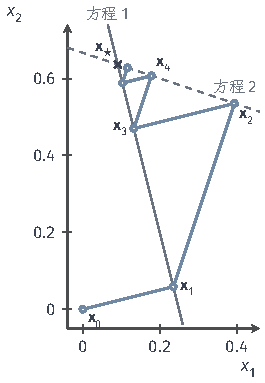
\includegraphics[width=44.81mm]{figures/01-basic-mathematics/03-vectors-matrices-and-multivariate-functions/tikz/c5-kaczmarz-projection-path/figure.pdf}
  \caption{循环Kaczmarz在贯穿例上的交替投影路径。实线为第一个方程$4x_1+x_2=1$的解集，虚线为第二个方程$x_1+3x_2=2$的解集；从$\bm x_0=\bm 0$出发依次垂直投影到两条直线上，折线连接精确计算的前六个迭代点并逐步收拢到交点$\bm x_\star$，图中标出前四个。坐标轴等比例，投影段与对应直线垂直。}
  \label{fig:ls-kaczmarz-projection-path}
\end{figure}

\paragraph{随机选行}
随机版本的投影公式不变，只是选行方式改为按$p_i$独立抽样，收敛结论因此是关于期望的。设方程相容，$\bm x_\star$如定理~\ref{thm:ls-kaczmarz-convergence}，误差$\bm\varepsilon_k$在行空间中。在给定$\bm\varepsilon_k$时对所选行求平均，由式~\eqref{eq:ls-kaczmarz-distance}，
\[
 \begin{aligned}
 \sum_{i=1}^mp_i\frac{(\bm a_i^\top\bm\varepsilon_k)^2}{\lVert\bm a_i\rVert_2^2}
 &=\frac{\lVert\bm A\bm\varepsilon_k\rVert_2^2}{\lVert\bm A\rVert_F^2}\\
 &\geq\frac{\sigma_r^2}{\lVert\bm A\rVert_F^2}\lVert\bm\varepsilon_k\rVert_2^2 ,
 \end{aligned}
\]
其中$\sigma_r$是最小正奇异值，不等号来自定理~\ref{thm:ls-svd-singular-value-norms}对$\ker\bm A$正交补的下界。所以一步之后误差平方的条件平均满足
\[
 \mathbb E\bigl[\lVert\bm\varepsilon_{k+1}\rVert_2^2\bigm|\bm\varepsilon_k\bigr]
 \leq\Bigl(1-\frac{\sigma_r^2}{\lVert\bm A\rVert_F^2}\Bigr)\lVert\bm\varepsilon_k\rVert_2^2 .
\]

选取概率与行的平方范数成正比，正是为了让分母$\lVert\bm a_i\rVert_2^2$被抵消，使这一平均化成$\lVert\bm A\bm\varepsilon_k\rVert_2^2$。

把这一步估计逐步叠加，得到
\begin{equation}
 \mathbb E\lVert\bm\varepsilon_k\rVert_2^2\leq\Bigl(1-\frac{\sigma_r^2}{\lVert\bm A\rVert_F^2}\Bigr)^k\lVert\bm\varepsilon_0\rVert_2^2 ;
 \label{eq:ls-kaczmarz-expected-rate}
\end{equation}
满列秩时这一结论由Strohmer与Vershynin给出\scite{math-strohmer2009randomized}。叠加时需要对此前各次选行的结果取条件期望，所用的随机变量与期望工具可参考\BookChapterRef{chap:random-variables}{卷七第2章“随机变量的分布”}。这里的结论是期望意义下的：单条轨迹上的误差每步不增，但不保证每一步都按这个因子缩小。

\paragraph{不相容情形}
不相容时情况不同。取$\bm A=(1,1)^\top$，$\bm b=(1,3)^\top$，未知量是标量，两行分别要求$x=1$和$x=3$。两行长度都为一，投影化为$x\gets b_i$，循环投影便在$1$与$3$之间往返，而最小二乘解是$\hat x=2$。随机选行时每一步$x$也只取$1$或$3$，所以仅改选行方式不能保证得到最小二乘解。不相容问题交给下一节的算法处理。

图~\ref{fig:solver-inconsistent-row-projections}画出了这个最小的不相容例。每次行投影都使一条方程成立，却始终跨过最小二乘折中点，因而需要校正右端。

\begin{figure}[!htb]
  \centering
  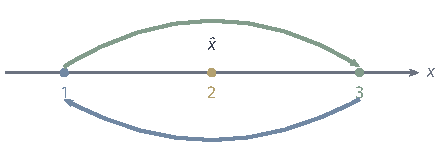
\includegraphics{figures/02-vectors-matrices-and-multivariate-calculus/03-linear-equations-and-optimization/tikz/learning-mechanisms/inconsistent-row-projections.pdf}
  \caption{循环行投影在不相容方程$x=1$、$x=3$之间往返。两条弧形箭头表示依次满足两行后的跳转；黄色点$\hat x=2$是最小二乘解，并非任何一次原始行投影的落点。}
  \label{fig:solver-inconsistent-row-projections}
\end{figure}

\section{扩展Kaczmarz算法}
\label{sec:ls-extended-kaczmarz}

上一节的例子说明，方程不相容时，行投影总在各行的解之间来回，原因是右端含有任何$\bm x$都拟合不了的部分。\term{扩展Kaczmarz算法}（extended Kaczmarz method）先用列投影逐步取出这一部分，再对校正后的相容方程作行投影，从而把Kaczmarz算法推广到一般的最小二乘问题。本节先推导这两种投影及其配合方式，再在上一节的不相容例上逐步执行，最后分析收敛与代价。

\subsection{主要思想}

要解的是最小二乘问题
\[
 \min_{\bm x}\lVert\bm b-\bm A\bm x\rVert_2 ,\qquad \bm A\in\mathbb R^{m\times d},
\]
方程$\bm A\bm x=\bm b$可以不相容，目标是其中范数最小的解$\bm A^\dagger\bm b$。上一节的行投影只适用于相容方程，所以先把问题改写成一个相容方程。

\paragraph{右端的分解}
由正交分解，
\begin{equation}
 \bm b=\bm b_\parallel+\bm b_\perp,\qquad \bm b_\parallel\in\operatorname{range}(\bm A),\quad \bm b_\perp\in\ker(\bm A^\top).
 \label{eq:ls-extended-kaczmarz-rhs-split}
\end{equation}
由第~\ref{sec:ls-ordinary-ls}节，最小二乘解就是相容方程$\bm A\bm x=\bm b_\parallel$的解，其中的最小范数解是$\bm A^\dagger\bm b$；$\bm b_\perp$则是任何$\bm x$都拟合不了的部分。

在不相容例$\bm A=(1,1)^\top$、$\bm b=(1,3)^\top$中，$\operatorname{range}(\bm A)$由$(1,1)^\top$张成。把$\bm b$投影到这条直线上，得
\[
 \bm b_\parallel=\frac{1+3}{2}\begin{bmatrix}1\\1\end{bmatrix}=\begin{bmatrix}2\\2\end{bmatrix}.
\]
剩下的部分是
\[
 \bm b_\perp=\bm b-\bm b_\parallel=\begin{bmatrix}-1\\1\end{bmatrix}.
\]
校正后的方程$\bm A x=\bm b_\parallel$两行都要求$x=2$，正是最小二乘解。

$\bm b_\perp$事先未知，所以引入一个$m$维辅助向量$\bm z$去逼近它，再求解$\bm A\bm x=\bm b-\bm z$。这样就要做两件事：用列的信息把$\bm z$推向$\bm b_\perp$，用行投影求解校正后的方程。

\paragraph{列投影}
$\bm b_\perp$在$\ker(\bm A^\top)$中，即满足$\bm A^\top\bm z=\bm0$：$\bm z$与每一列正交。记第$j$列为$\bm c_j$，这是$d$个齐次方程$\bm c_j^\top\bm z=0$组成的相容方程组，未知量是$\bm z$。把上一节的最短修正用于其中一个方程，就得到一次列投影。

在不相容例中只有一列$\bm c_1=(1,1)^\top$，$\lVert\bm c_1\rVert_2^2=2$。对$\bm z=(z_1,z_2)^\top$，方程的残差为$0-\bm c_1^\top\bm z=-(z_1+z_2)$，最短修正给出
\[
 \bm z-\frac{z_1+z_2}{2}\begin{bmatrix}1\\1\end{bmatrix}
 =\frac12\begin{bmatrix}z_1-z_2\\z_2-z_1\end{bmatrix},
\]
即从每个分量中减去两分量的平均值。从$\bm z=\bm b=(1,3)^\top$出发，一次列投影就得到$(-1,1)^\top=\bm b_\perp$。

一般地，对当前的$\bm z_k$和所选的列$j$，列投影为
\begin{equation}
 \bm z_{k+1}=\bm z_k-\frac{\bm c_j^\top\bm z_k}{\lVert\bm c_j\rVert_2^2}\,\bm c_j .
 \label{eq:ls-extended-kaczmarz-column}
\end{equation}
式中$\bm c_j^\top\bm z_k$衡量$\bm z_k$与第$j$列偏离正交的程度；除以$\lVert\bm c_j\rVert_2^2$换算成沿$\bm c_j$的系数；减去这个倍数之后，$\bm c_j^\top\bm z_{k+1}=0$。它就是对相容方程$\bm A^\top\bm z=\bm0$作一次Kaczmarz投影。

从$\bm z_0=\bm b$出发，每次减去的都是某一列的倍数，属于$\operatorname{range}(\bm A)$。所以$\bm z_k$在$\ker(\bm A^\top)$中的分量始终是$\bm b_\perp$，变化的只是列空间中的部分$\bm z_k-\bm b_\perp$；同时$\bm b-\bm z_k$始终在$\operatorname{range}(\bm A)$中，校正后的方程$\bm A\bm x=\bm b-\bm z_k$始终相容。

\paragraph{校正后的行投影}
若校正量为$\bm z_k$，第$i$条目标方程就是$\bm a_i^\top\bm x=b_i-(\bm z_k)_i$。沿用式~\eqref{eq:ls-kaczmarz-update}的推导，只需把右端$b_i$换成$b_i-(\bm z_k)_i$，得到行投影
\begin{equation}
 \bm x_{k+1}=\bm x_k+\frac{b_i-(\bm z_k)_i-\bm a_i^\top\bm x_k}{\lVert\bm a_i\rVert_2^2}\,\bm a_i .
 \label{eq:ls-extended-kaczmarz-row}
\end{equation}
分子是校正方程第$i$行的行残差，其余与标准Kaczmarz相同。

在不相容例中$\bm a_i=1$，$\lVert\bm a_i\rVert_2^2=1$，行投影化为$x\gets b_i-(\bm z_k)_i$。不作校正（$\bm z=\bm0$）时这就是$x\gets b_i$，在$1$与$3$之间往返；以$\bm z=\bm b_\perp=(-1,1)^\top$校正后，两行分别给出
\[
 1-(-1)=2,\qquad 3-1=2 ,
\]
两行一致，都得到最小二乘解$x=2$。

\paragraph{两种投影的配合}
实际计算中$\bm z_k$只是$\bm b_\perp$的近似，两种投影交替进行。本章采用同步读取轮初状态的版本：每轮的$\bm z_{k+1}$和$\bm x_{k+1}$都由$(\bm z_k,\bm x_k)$计算，行更新不改用刚得到的$\bm z_{k+1}$。先更新$\bm z$、再用新的$\bm z$更新$\bm x$的版本也可以使用，但两种时间顺序产生不同的数值轨迹，实现应与所用的收敛分析一致。行与列的选取沿用上一节的随机规则，这里采用Zouzias与Freris的随机版本\scite{math-zouzias2013randomized}。

于是误差有两个来源。列投影缩小$\bm z_k-\bm b_\perp$；行投影则是在右端仍受这一误差扰动时逼近$\bm A\bm x=\bm b_\parallel$。取$\bm x_0=\bm0$，且每步都沿行方向修正，保证$\bm x_k$始终在行空间中，最终选出最小范数代表。

\subsection{算法实现}

按上一小节的推导，扩展Kaczmarz算法每轮抽取一行和一列，作一次列投影和一次行投影，两者都读取轮初状态；每隔规定的轮数检查两项判据。输入为$\bm A,\bm b$，输出为$\bm x$；超参数为绝对容差$\mathrm{atol}$、相对容差$\mathrm{rtol}$和轮数上限$K$。下面写出变量、初始化与每轮更新。

下面用上一节不相容例的数据逐步演示：
\[
 \bm A=\begin{bmatrix}1\\1\end{bmatrix},\qquad \bm b=\begin{bmatrix}1\\3\end{bmatrix}.
\]
例中取$\mathrm{atol}=0$、$\mathrm{rtol}=0.1$，每轮都作检查。

\paragraph{变量}
\begin{itemize}
 \item $\bm x\in\mathbb R^d$：当前近似解$\bm x_k$。
 \item $\bm z\in\mathbb R^m$：辅助向量$\bm z_k$，逼近不可拟合的部分$\bm b_\perp$；它只是内部状态，不作为输出。
 \item $\lVert\bm a_i\rVert_2^2$与$\lVert\bm c_j\rVert_2^2$：各行、各列的平方范数，预先算好，同时用作抽样权重。
 \item $i_k,j_k$：第$k$轮抽到的行与列。
 \item $\eta_k,\gamma_k$：列投影与行投影的系数，用后即弃。
 \item $k$：轮次，从$0$开始。
\end{itemize}

\paragraph{初始化}
若$\bm A=\bm0$，直接返回最小范数解$\bm x=\bm0$。否则预存各行、各列的平方范数，得到抽样概率
\begin{equation}
 p_i=\frac{\lVert\bm a_i\rVert_2^2}{\lVert\bm A\rVert_F^2},\qquad
 q_j=\frac{\lVert\bm c_j\rVert_2^2}{\lVert\bm A\rVert_F^2};
 \label{eq:ls-extended-kaczmarz-sampling}
\end{equation}
零行和零列的概率为零，不会被抽到，也就不会出现除以零。再把内部状态初始化为
\[
 \bm x_0=\bm0,\qquad \bm z_0=\bm b,\qquad k=0 .
\]
两项判据的阈值按各自的尺度取为
\begin{equation}
 \tau_r=\mathrm{atol}+\mathrm{rtol}\lVert\bm b\rVert_2,\qquad
 \tau_n=\mathrm{atol}+\mathrm{rtol}\lVert\bm A\rVert_F\lVert\bm b\rVert_2 ,
 \label{eq:ls-extended-kaczmarz-thresholds}
\end{equation}
后者的尺度来自$\lVert\bm A^\top\bm z_0\rVert_2=\lVert\bm A^\top\bm b\rVert_2\leq\lVert\bm A\rVert_F\lVert\bm b\rVert_2$。

例中两行的平方范数都为$1$，唯一一列的平方范数为$2$，$\lVert\bm A\rVert_F=\sqrt2$，$\lVert\bm b\rVert_2=\sqrt{10}$，于是
\[
 p_1=p_2=\frac12,\qquad q_1=1 .
\]
两项阈值为
\[
 \tau_r=\frac{\sqrt{10}}{10}\approx0.316,\qquad \tau_n=\frac{\sqrt{20}}{10}\approx0.447 .
\]
初始时$\bm b-\bm z_0-\bm A x_0=\bm0$，但
\[
 \bm A^\top\bm z_0=1+3=4>\tau_n ,
\]
所以进入第一轮。

\paragraph{每轮更新}
在第$k$轮：
\begin{enumerate}
 \item \textbf{抽样。}按概率$p_i$与$q_j$独立抽取行$i_k$和列$j_k$，并记录抽到的行列序列，以便复算同一条轨迹。例中每轮都取$j_k=1$，行$i_k$以各一半的概率取$1$或$2$；下面会看到，两种情况结果相同。

 \item \textbf{列投影。}保存轮初状态$(\bm x_k,\bm z_k)$，按式~\eqref{eq:ls-extended-kaczmarz-column}计算
 \[
  \eta_k=\frac{\bm c_{j_k}^\top\bm z_k}{\lVert\bm c_{j_k}\rVert_2^2},\qquad \bm z_{k+1}=\bm z_k-\eta_k\bm c_{j_k},
 \]
 旧的$\bm z_k$保留给本轮的行投影使用。例中第一轮
 \[
  \eta_0=\frac{1+3}{2}=2 .
 \]
 列投影后的辅助向量为
 \[
  \bm z_1=\begin{bmatrix}1\\3\end{bmatrix}-2\begin{bmatrix}1\\1\end{bmatrix}=\begin{bmatrix}-1\\1\end{bmatrix},
 \]
 已经等于$\bm b_\perp$。

 \item \textbf{行投影。}仍读取旧的$(\bm z_k)_{i_k}$，按式~\eqref{eq:ls-extended-kaczmarz-row}计算
 \[
 \begin{aligned}
  \gamma_k&=\frac{b_{i_k}-(\bm z_k)_{i_k}-\bm a_{i_k}^\top\bm x_k}{\lVert\bm a_{i_k}\rVert_2^2},\\
  \bm x_{k+1}&=\bm x_k+\gamma_k\bm a_{i_k}.
 \end{aligned}
 \]
 例中第一轮用的是$\bm z_0=\bm b$，无论抽到哪一行，分子都是$b_i-b_i-0=0$，所以
 \[
  \gamma_0=0,\qquad x_1=0 ,
 \]
 $x$不动。若行投影改用新的$\bm z_1$，这一步就会提前得到$x=2$；同步版本不这样做。

 \item \textbf{替换状态。}以$(\bm x_{k+1},\bm z_{k+1})$同时替换旧状态，令$k\leftarrow k+1$。

 例中第二轮的列内积为$-1+1=0$，所以
 \[
  \eta_1=0,\qquad \bm z_2=\bm z_1=\begin{bmatrix}-1\\1\end{bmatrix}.
 \]
 行投影读取$\bm z_1$，抽到第一行或第二行时分别得到
 \[
  \gamma_1=1-(-1)-0=2,\qquad \gamma_1=3-1-0=2 .
 \]
 两种情况都得到
 \[
  x_2=2 ,
 \]
 此后不再改变。

 \item \textbf{停止。}在规定的检查轮次，若
 \begin{equation}
  \lVert\bm b-\bm z_k-\bm A\bm x_k\rVert_2\leq\tau_r
  \quad\text{且}\quad
  \lVert\bm A^\top\bm z_k\rVert_2\leq\tau_n ,
  \label{eq:ls-extended-kaczmarz-stopping}
 \end{equation}
 就以“达到容差”结束；若已做满$K$轮，以“次数耗尽”结束；两种情况都取$\bm x=\bm x_k$。

 前一项检查$\bm x_k$对校正方程的拟合，后一项检查辅助向量与列空间的正交性，两项都只是内部停止判据，检查值不作为输出。宣布达到容差之前，再直接计算正规残差$\bm A^\top(\bm b-\bm A\bm x_k)$复核；不要求原残差$\lVert\bm b-\bm A\bm x_k\rVert_2$趋于零。

 例中第一轮后
 \[
  \bm b-\bm z_1-\bm A x_1=\begin{bmatrix}2\\2\end{bmatrix},\qquad \bm A^\top\bm z_1=0 ,
 \]
 后一项已满足，前一项的长度$2\sqrt2\approx2.83$仍大于$\tau_r$，继续。第二轮后
 \[
  \bm b-\bm z_2-\bm A x_2=\bm0,\qquad \bm A^\top\bm z_2=0 ,
 \]
 两项都满足。再复核正规残差，
 \[
  \bm A^\top(\bm b-\bm A x_2)=(1-2)+(3-2)=0 ,
 \]
 以“达到容差”结束。
\end{enumerate}

最终得到
\[
 x_2=2 .
\]
原残差$\bm b-\bm A x_2=(-1,1)^\top$不为零，残差平方和为$2$，正是$\min_x\bigl[(x-1)^2+(x-3)^2\bigr]$的最优值：原方程依然没有精确解，但$x_2=2$已经是最小二乘解。

这个例子也说明两项判据缺一不可：第一轮后$\bm z$已经正确，$x$却还没有移动。

\subsection{算法分析}

\paragraph{极限的含义}
列投影只减去列的倍数，保留$\bm b$的正交残差分量$\bm b_\perp$，同时缩小$\bm z_k-\bm b_\perp$；零初值和沿行方向的修正又使$\bm x_k$始终留在行空间中。当$\bm z_k$趋于$\bm b_\perp$时，行投影求解的就是相容方程$\bm A\bm x=\bm b_\parallel$，而它在行空间中的唯一解是$\bm A^\dagger\bm b$，所以这一构造指向最小范数最小二乘解。

\paragraph{列校正的收敛}
列投影是对相容方程$\bm A^\top\bm z=\bm 0$作Kaczmarz投影，初值为$\bm b$。由定理~\ref{thm:ls-kaczmarz-convergence}（对$\bm A^\top$应用），按固定循环顺序选列时，$\bm z_k$收敛到$\bm b$在$\ker(\bm A^\top)$上的正交投影，即$\bm b_\perp$，每轮按小于一的因子几何收缩。随机选列时，上一节的一步平均估计同样适用于$\bm z_k-\bm b_\perp$，它属于$\operatorname{range}(\bm A)$，平均缩小因子为$1-\sigma_r^2/\lVert\bm A\rVert_F^2$。

\paragraph{行迭代的误差递推}
令$\bm x_\star=\bm A^\dagger\bm b$，它满足$\bm A\bm x_\star=\bm b_\parallel=\bm b-\bm b_\perp$，故$b_i=\bm a_i^\top\bm x_\star+(\bm b_\perp)_i$。代入行投影，误差$\bm\varepsilon_k=\bm x_k-\bm x_\star$满足
\begin{equation}
 \bm\varepsilon_{k+1}=\bm P_{i_k}\bm\varepsilon_k+\frac{(\bm b_\perp-\bm z_k)_{i_k}}{\lVert\bm a_{i_k}\rVert_2^2}\,\bm a_{i_k}.
 \label{eq:ls-extended-kaczmarz-error-recursion}
\end{equation}
第一项是标准Kaczmarz的误差映射，第二项是校正误差带来的扰动，长度不超过$\lVert\bm z_k-\bm b_\perp\rVert_2/\lVert\bm a_{i_k}\rVert_2$。$\bm\varepsilon_k$始终在行空间中。

在循环版本中，把一轮行扫掠合起来，有
\begin{equation}
 \lVert\bm\varepsilon_{\text{轮末}}\rVert_2\leq q\lVert\bm\varepsilon_{\text{轮初}}\rVert_2+\varphi ,
 \label{eq:ls-extended-kaczmarz-sweep-bound}
\end{equation}
其中$q<1$是定理~\ref{thm:ls-kaczmarz-convergence}中的因子，$\varphi$是本轮各步扰动长度之和，随$\bm z_k\to\bm b_\perp$趋于零。由这一递推，轮末误差有界；记其上极限为$L$，则$L\leq qL$，故$L=0$，即$\bm x_k\to\bm A^\dagger\bm b$。

随机版本在规定的独立抽样下，期望平方误差以由$1-\sigma_r^2/\lVert\bm A\rVert_F^2$决定的几何速率趋于零\scite{math-zouzias2013randomized}，证明同样要用条件期望。这里不宣称每条轨迹的原残差逐步下降，算法实现的例子中第一轮$x$就完全没有移动。

\paragraph{代价}
每轮访问一行、一列，并保存长度为$m$的$\bm z_k$，代价按访问的非零元个数计算；停止检查需要计算$\bm A\bm x_k$与$\bm A^\top\bm z_k$，各相当于一次完整的矩阵乘向量，所以只按规定间隔进行。数值敏感性仍受原问题小奇异值的影响：两种收缩因子都由$\sigma_r^2/\lVert\bm A\rVert_F^2$决定，它很小时收敛很慢。

\section{本章小结}
\label{sec:row-projection-summary}

本章回答了只能逐行或逐列访问数据时怎样求解线性方程。Kaczmarz算法每次只满足一个方程：由最短修正原理，更新沿所选行的法向进行，系数由行残差除以行的平方范数确定，新点是当前点到该超平面的正交投影。方程相容时，每一步到每个精确解的距离都不增；循环版本每轮按小于一的因子收缩，收敛到$\bm A^\dagger\bm b$加上初值的零空间分量，零初值时就是最小范数解。随机版本按行的平方范数抽样，期望平方误差以$1-\sigma_r^2/\lVert\bm A\rVert_F^2$为因子几何减小。

使用时要注意几个条件。行之间越接近平行，收敛越慢；零行对应非零右端说明方程不相容，必须单独处理；某一行的残差为零不说明求解完成。方程不相容时，标准Kaczmarz在各行的解之间往返，无论循环还是随机选行，都不会停在最小二乘解上。

扩展Kaczmarz算法把右端分成可拟合与不可拟合两部分：列投影从$\bm z_0=\bm b$出发逼近不可拟合的$\bm b_\perp$，行投影求解校正后的相容方程$\bm A\bm x=\bm b-\bm z$。本章采用同步版本，两种投影都读取轮初状态；零初值保证极限是最小范数最小二乘解。

检验时，标准算法看全部方程的原残差；扩展算法看$\lVert\bm A^\top\bm z\rVert_2$与校正方程的残差，并复核正规残差，原残差最终非零是正常的。两种算法的最小范数性质都依赖零初值和行空间保持，不由残差判据保证。它们每步只读一行或一列，代价低，但收敛速度受$\sigma_r^2/\lVert\bm A\rVert_F^2$限制；误差解释与方法比较在第~\ref{chap:solution-error-regularization}章进行。

\chapter{求解误差、正则化与方法选择}
\label{chap:solution-error-regularization}

前几章给出了多条求解路线：直接分解、定常迭代、Krylov子空间法与行列投影法。每条路线最后都交出一个向量，但交出来的向量并不都同样可信。设两列几乎平行的矩阵配上略有误差的观测：精确地解出方程，系数可能离真实值很远；换成另一种算法，可能连这个精确解也没有算准；迭代法提前停下，又多出一份截断误差。即使残差已经很小，也不能直接断言系数可靠。

本章回答三个问题：算出的解能相信多少，问题本身太敏感时怎么办，以及在多种方法都可用时怎样选择。

第~\ref{sec:ls-numerical-sensitivity}节先把误差的来源分开。数据误差经问题本身放大，用有限扰动界与条件数度量；近似解的质量用残差、前向误差与后向误差判断；最小二乘的系数、拟合值与残差敏感程度不同；矩阵的秩一旦变化，伪逆可能不连续，数值秩要结合误差水平确定。这里用到第~\ref{chap:condition-and-spectral-perturbation}章的条件数与奇异值扰动界，以及第~\ref{chap:linear-solution-selection}章的伪逆与选解。

第~\ref{sec:ls-truncated-svd-ridge}节处理敏感性本身无法由算法消除的情形。岭回归与Tikhonov正则化在目标中加入惩罚，谱截断正则化舍弃小奇异值方向，二者都主动改变求解目标，用拟合误差与偏差换取稳定。截断所用矩阵的最佳低秩性质留到第~\ref{chap:matrix-approximation}章。

第~\ref{sec:ls-method-selection}节在前两节建立的误差标准下，把第~\ref{chap:direct-linear-solvers}—\ref{chap:row-projection-methods}章的方法放回同一组问题中比较：先确定求解目标，再看矩阵条件、计算开销与收敛速度、数值稳定性，最后给出典型问题的取舍。本章的误差分析都针对有限大小的扰动；扰动趋于零时的局部线性化观点在第~\ref{chap:differential-perturbation-analysis}章讨论。

\section{解的误差与敏感性}
\label{sec:ls-numerical-sensitivity}

求解目标确定、算法也给出结果以后，还要回答算出的结果能相信多少。本节分四方面讨论：数据的扰动怎样传到解，算出的近似解怎样用残差判断，最小二乘的不同输出各有多敏感，以及矩阵的秩变化时伪逆怎样变化。

讨论每种误差，都要先说清以什么为参照、允许修改哪些数据。比较两个精确解时，修改的是$\bm A$或$\bm b$，参照是原问题的精确解。用残差判断近似解时，数据不改，参照是未知的真解。后向误差则反过来问：数据至少要改多少，近似解才成为修改后问题的精确解。

以下结论都由精确方程、范数估计和奇异值性质建立，扰动可以有有限大小；所用的条件数与奇异值扰动界来自第~\ref{chap:condition-and-spectral-perturbation}章。扰动趋于零时的局部观点留到后文：第~\ref{chap:matrix-differentiation}章建立逆矩阵等运算的微分公式，第~\ref{chap:differential-perturbation-analysis}章再从同样的精确关系中提取解映射的一阶响应，讨论局部条件数与一阶近似的余项。

\subsection{系数矩阵与右端项的扰动}
\label{sec:ls-equation-sensitivity}

方程的数据常常来自测量或前一步计算，本身就带有误差。本小节回答：数据改变一点，方程的精确解改变多少。这里比较的是两个精确解，与算法和舍入无关，所以放大完全来自问题本身。

本小节设$\bm A\in\mathbb R^{d\times d}$可逆，$\bm b\ne\bm0$，精确解为$\bm x_\star=\bm A^{-1}\bm b$。向量范数与它诱导的矩阵范数始终取同一种，记
\[
 \kappa(\bm A)=\lVert\bm A\rVert\,\lVert\bm A^{-1}\rVert .
\]
用二范数时写作$\kappa_2(\bm A)$。

\paragraph{右端扰动}
先固定$\bm A$，只把右端改为$\bm b+\Delta\bm b$，记新解为$\bm x_\star+\Delta\bm x$。我们关心的是解的相对变化与右端的相对变化之比，它说明右端的误差被放大了多少倍。

新旧两个方程分别为
\[
 \bm A(\bm x_\star+\Delta\bm x)=\bm b+\Delta\bm b,\qquad \bm A\bm x_\star=\bm b .
\]
两式相减，得到
\begin{equation}
 \bm A\,\Delta\bm x=\Delta\bm b,\qquad\text{即}\qquad \Delta\bm x=\bm A^{-1}\Delta\bm b .
 \label{eq:ls-rhs-perturbation-exact}
\end{equation}
推导中没有任何近似，所以这个关系对任意大小的$\Delta\bm b$都精确成立。

对它取范数，得到解的绝对变化的界
\[
 \lVert\Delta\bm x\rVert\leq\lVert\bm A^{-1}\rVert\,\lVert\Delta\bm b\rVert .
\]
要换成相对变化，还需要用$\lVert\bm b\rVert$估计$\lVert\bm x_\star\rVert$。由$\bm b=\bm A\bm x_\star$，
\[
 \lVert\bm b\rVert\leq\lVert\bm A\rVert\,\lVert\bm x_\star\rVert,\qquad\text{即}\qquad \frac1{\lVert\bm x_\star\rVert}\leq\frac{\lVert\bm A\rVert}{\lVert\bm b\rVert}.
\]
两个不等式相乘，得到相对误差界
\begin{equation}
 \frac{\lVert\Delta\bm x\rVert}{\lVert\bm x_\star\rVert}\leq\kappa(\bm A)\,\frac{\lVert\Delta\bm b\rVert}{\lVert\bm b\rVert}.
 \label{eq:ls-rhs-relative-error-bound}
\end{equation}
这就是第~\ref{sec:ls-matrix-condition-number}节的条件数界（定理~\ref{thm:matrix-analysis-condition-number-bound}）：条件数是右端相对误差的最大放大倍数。

哪些方向上的右端误差放大得最多，可以由奇异值分解读出。设$\bm A=\sum_{i=1}^d\sigma_i\bm u_i\bm v_i^\top$，把右端的变化按左奇异向量展开，
\[
 \Delta\bm b=\sum_{i=1}^d\beta_i\bm u_i,\qquad \beta_i=\bm u_i^\top\Delta\bm b .
\]
由于$\bm A^{-1}=\sum_i\sigma_i^{-1}\bm v_i\bm u_i^\top$，解的变化为
\begin{equation}
 \Delta\bm x=\bm A^{-1}\Delta\bm b=\sum_{i=1}^d\frac{\beta_i}{\sigma_i}\,\bm v_i .
 \label{eq:ls-rhs-perturbation-svd}
\end{equation}
沿$\bm u_i$的误差分量被放大$1/\sigma_i$倍，并转到$\bm v_i$方向上。误差落在最小奇异值对应的方向上时，放大最多。下面的例子在精确算术中计算，比较一个良态矩阵和一个两列接近同向的矩阵。

\begin{example}[良态矩阵与近平行列矩阵]
\label{ex:ls-rhs-perturbation-near-parallel}
先看一个良态的对照，取以下数据：
\[
 \bm A_1=\begin{bmatrix}2&0\\0&1\end{bmatrix},\qquad \bm b=\begin{bmatrix}2\\1\end{bmatrix}.
\]
精确解为$\bm x_\star=(1,1)^\top$，$\kappa_2(\bm A_1)=2$。把右端的第二个分量改为$1.01$，即$\Delta\bm b=(0,0.01)^\top$，则解的变化为
\[
 \Delta\bm x=\bm A_1^{-1}\Delta\bm b=\begin{bmatrix}0\\0.01\end{bmatrix},
\]
新解为$(1,1.01)^\top$。右端与解的相对变化分别为
\[
 \frac{\lVert\Delta\bm b\rVert_2}{\lVert\bm b\rVert_2}=\frac{0.01}{\sqrt5}\approx0.00447,\qquad
 \frac{\lVert\Delta\bm x\rVert_2}{\lVert\bm x_\star\rVert_2}=\frac{0.01}{\sqrt2}\approx0.00707,
\]
放大约$1.58$倍，不超过$\kappa_2(\bm A_1)=2$。

再取两列接近同向的矩阵
\[
 \bm A_2=\begin{bmatrix}1&1\\0&\varepsilon\end{bmatrix},\qquad \varepsilon=10^{-2},
\]
它的逆矩阵为
\[
 \bm A_2^{-1}=\begin{bmatrix}1&-1/\varepsilon\\0&1/\varepsilon\end{bmatrix}.
\]
右端取$\bm b=(2,0)^\top$，解为$\bm x_\star=(2,0)^\top$。把右端的第二个分量改为$\eta$，解的变化按元素为
\[
 \Delta\bm x=\bm A_2^{-1}\begin{bmatrix}0\\\eta\end{bmatrix}=\begin{bmatrix}-\eta/\varepsilon\\\eta/\varepsilon\end{bmatrix}.
\]
取$\eta=0.01$，得$\Delta\bm x=(-1,1)^\top$，解由$(2,0)^\top$变为$(1,1)^\top$。右端与解的相对变化分别为
\[
 \frac{\lVert\Delta\bm b\rVert_2}{\lVert\bm b\rVert_2}=\frac{0.01}{2}=0.005,\qquad
 \frac{\lVert\Delta\bm x\rVert_2}{\lVert\bm x_\star\rVert_2}=\frac{\sqrt2}{2}\approx0.707,
\]
放大约$141$倍。

这个倍数可以与条件数比较。$\bm A_2^\top\bm A_2=\left[\begin{smallmatrix}1&1\\1&1+\varepsilon^2\end{smallmatrix}\right]$的特征值是$\sigma_{\max}^2$与$\sigma_{\min}^2$，由迹与行列式得
\[
 \sigma_{\max}^2+\sigma_{\min}^2=2+\varepsilon^2,\qquad \sigma_{\max}\sigma_{\min}=\varepsilon .
\]
解出
\[
 \sigma_{\max}\approx1.41423,\qquad \sigma_{\min}\approx0.0070710,
\]
所以$\kappa_2(\bm A_2)\approx200$。

实际倍数$141$没有达到$200$，差别来自$\bm b$：界中用$\lVert\bm A_2\rVert_2\approx1.414$估计$\lVert\bm b\rVert_2/\lVert\bm x_\star\rVert_2$，而这里该比值为$1$。

放大的方向也可以由奇异向量看出。数值计算给出
\[
 \bm v_{\min}\approx\begin{bmatrix}0.7071\\-0.7071\end{bmatrix},\qquad
 \bm u_{\min}\approx\begin{bmatrix}0.0050\\-1.0000\end{bmatrix}.
\]
$\Delta\bm b=(0,0.01)^\top$几乎全部落在$\bm u_{\min}$上，系数$\beta_{\min}\approx-0.0100$，而沿另一方向的系数只有约$5\times10^{-5}$。于是
\[
 \Delta\bm x\approx\frac{\beta_{\min}}{\sigma_{\min}}\,\bm v_{\min}\approx-1.4142\,\bm v_{\min}\approx\begin{bmatrix}-1\\1\end{bmatrix}.
\]
解的变化正沿着$\bm v_{\min}$，两个系数此增彼减。图~\ref{fig:matrix-analysis-coefficient-sensitivity}画出了$\varepsilon$减小时这种分裂怎样加剧。
\end{example}

\begin{figure}
 \centering
 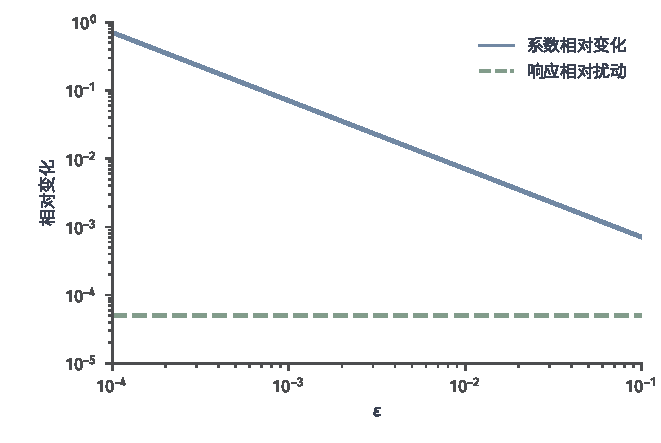
\includegraphics[width=0.92\linewidth]{figures/00-shared/mathematical-preliminaries-upper/02-linear-spaces/matplotlib/matrix-analysis-coefficient-sensitivity/figure.pdf}
 \caption{近平行列的系数分裂。取$\bm A_2=\left[\begin{smallmatrix}1&1\\0&\varepsilon\end{smallmatrix}\right]$、$\bm b=(2,0)^\top$，固定右端扰动$\Delta\bm b=(0,10^{-4})^\top$。蓝线为系数相对变化$\lVert\Delta\bm x\rVert_2/\lVert\bm x\rVert_2$，绿虚线为右端相对扰动$\lVert\Delta\bm b\rVert_2/\lVert\bm b\rVert_2$。两个系数沿相反方向偏离$(2,0)^\top$，变化量随$1/\varepsilon$增长。}
 \label{fig:matrix-analysis-coefficient-sensitivity}
\end{figure}

\paragraph{系数矩阵的扰动}
\label{sec:ls-inverse-sensitivity}%
系数矩阵的元素也可能带误差。设扰动后的矩阵为$\bm B=\bm A+\bm E$。与右端扰动不同，这时会出现一个新问题：$\bm B$甚至可能不可逆，例如$\bm E=-\bm A$。所以要先确定扰动多小时$\bm B$一定可逆，再估计$\bm B^{-1}$离$\bm A^{-1}$多远。

直观地看，$\bm E$是否算“小”，不能只看它本身的大小，还要看$\bm A$离奇异有多远。$\bm A^{-1}$的范数越大，$\bm A$越接近奇异，能容忍的扰动越小。下面的定理用乘积$\bm A^{-1}\bm E$或$\lVert\bm A^{-1}\rVert\lVert\bm E\rVert$来衡量扰动。

\begin{theorem}[逆矩阵的有限扰动]
\label{thm:ls-inverse-finite-perturbation}
设$\bm A\in\mathbb R^{d\times d}$可逆，$\bm B=\bm A+\bm E$。
\begin{enumerate}
 \item 若$\lVert\bm A^{-1}\bm E\rVert<1$，则$\bm B$可逆，
 \begin{equation}
  \lVert\bm B^{-1}\rVert\leq\frac{\lVert\bm A^{-1}\rVert}{1-\lVert\bm A^{-1}\bm E\rVert},
  \label{eq:ls-inverse-norm-bound}
 \end{equation}
 且
 \begin{equation}
  \bm B^{-1}-\bm A^{-1}=-\bm B^{-1}\bm E\,\bm A^{-1}.
  \label{eq:ch06-inverse-finite-perturbation}
 \end{equation}
 \item 若$q=\lVert\bm A^{-1}\rVert\lVert\bm E\rVert<1$，则第1条适用，并且
 \begin{equation}
  \frac{\lVert\bm B^{-1}-\bm A^{-1}\rVert}{\lVert\bm A^{-1}\rVert}
  \leq\frac{q}{1-q},\qquad q=\kappa(\bm A)\frac{\lVert\bm E\rVert}{\lVert\bm A\rVert}.
  \label{eq:ls-inverse-relative-perturbation-bound}
 \end{equation}
\end{enumerate}
\end{theorem}
\begin{proof}
先证第1条中的可逆性。设$\bm B\bm x=\bm0$，即$\bm A\bm x=-\bm E\bm x$，两边左乘$\bm A^{-1}$并取范数，
\[
 \bm x=-\bm A^{-1}\bm E\bm x,\qquad \lVert\bm x\rVert\leq\lVert\bm A^{-1}\bm E\rVert\,\lVert\bm x\rVert .
\]
由于$\lVert\bm A^{-1}\bm E\rVert<1$，只能$\lVert\bm x\rVert=0$。方阵$\bm B$的零空间只含零向量，故$\bm B$可逆。

再估计$\lVert\bm B^{-1}\rVert$。对任意$\bm y$，令$\bm x=\bm B^{-1}\bm y$，则$\bm A\bm x+\bm E\bm x=\bm y$。左乘$\bm A^{-1}$并取范数，
\[
 \begin{gathered}
 \bm x=\bm A^{-1}\bm y-\bm A^{-1}\bm E\bm x,\\
 \lVert\bm x\rVert\leq\lVert\bm A^{-1}\rVert\,\lVert\bm y\rVert+\lVert\bm A^{-1}\bm E\rVert\,\lVert\bm x\rVert .
 \end{gathered}
\]
把含$\lVert\bm x\rVert$的项移到左边，
\[
 \bigl(1-\lVert\bm A^{-1}\bm E\rVert\bigr)\lVert\bm B^{-1}\bm y\rVert\leq\lVert\bm A^{-1}\rVert\,\lVert\bm y\rVert .
\]
对所有$\lVert\bm y\rVert=1$取上确界，即得$\lVert\bm B^{-1}\rVert$的界。恒等式由$\bm A-\bm B=-\bm E$得到：
\[
 \begin{aligned}
 \bm B^{-1}-\bm A^{-1}&=\bm B^{-1}\bm A\bm A^{-1}-\bm B^{-1}\bm B\bm A^{-1}\\
 &=\bm B^{-1}(\bm A-\bm B)\bm A^{-1}=-\bm B^{-1}\bm E\bm A^{-1}.
 \end{aligned}
\]

第2条中，$\lVert\bm A^{-1}\bm E\rVert\leq\lVert\bm A^{-1}\rVert\lVert\bm E\rVert=q<1$，所以第1条适用，并有$\lVert\bm B^{-1}\rVert\leq\lVert\bm A^{-1}\rVert/(1-q)$。对式~\eqref{eq:ch06-inverse-finite-perturbation}取范数，
\[
 \begin{aligned}
 \lVert\bm B^{-1}-\bm A^{-1}\rVert&\leq\lVert\bm B^{-1}\rVert\,\lVert\bm E\rVert\,\lVert\bm A^{-1}\rVert\\
 &\leq\frac{\lVert\bm A^{-1}\rVert^2\lVert\bm E\rVert}{1-q}=\frac{q}{1-q}\,\lVert\bm A^{-1}\rVert .
 \end{aligned}
\]
两边除以$\lVert\bm A^{-1}\rVert$即得。最后，
\[
 q=\lVert\bm A\rVert\lVert\bm A^{-1}\rVert\cdot\frac{\lVert\bm E\rVert}{\lVert\bm A\rVert}=\kappa(\bm A)\frac{\lVert\bm E\rVert}{\lVert\bm A\rVert}.
\]
\end{proof}

界的分子$q$是条件数乘矩阵的相对扰动，分母$1-q$是到可逆性保证边界的余量。$q$越接近$1$，余量越小，界就越大。

\begin{example}[一次系数扰动]
\label{ex:ls-inverse-perturbation-numeric}
取示例~\ref{ex:ls-stationary-running-example}的矩阵，并只扰动它的右下角元素：
\[
 \bm A=\begin{bmatrix}4&1\\1&3\end{bmatrix},\qquad
 \bm E=\begin{bmatrix}0&0\\0&1/2\end{bmatrix}.
\]
扰动后的矩阵为
\[
 \bm B=\bm A+\bm E=\begin{bmatrix}4&1\\1&7/2\end{bmatrix}.
\]
两个逆矩阵分别为
\[
 \bm A^{-1}=\frac1{11}\begin{bmatrix}3&-1\\-1&4\end{bmatrix},\qquad
 \bm B^{-1}=\frac1{26}\begin{bmatrix}7&-2\\-2&8\end{bmatrix}.
\]
直接相减，得
\[
 \bm B^{-1}-\bm A^{-1}=\frac1{286}\begin{bmatrix}-1&4\\4&-16\end{bmatrix}.
\]
按恒等式~\eqref{eq:ch06-inverse-finite-perturbation}计算$-\bm B^{-1}\bm E\bm A^{-1}$，得到同一个矩阵。它是一个秩一矩阵，
\[
 \bm B^{-1}-\bm A^{-1}=-\frac1{286}\begin{bmatrix}1\\-4\end{bmatrix}\begin{bmatrix}1&-4\end{bmatrix},
\]
谱范数为$17/286\approx0.0594$。

在谱范数下，$\bm A$的特征值为$(7\pm\sqrt5)/2$，所以
\[
 \lVert\bm A\rVert_2\approx4.618,\qquad \lVert\bm A^{-1}\rVert_2\approx0.4198,\qquad \kappa_2(\bm A)\approx1.939 .
\]
于是
\[
 q=\lVert\bm A^{-1}\rVert_2\lVert\bm E\rVert_2\approx0.4198\times0.5\approx0.210 .
\]
定理给出的界与实际的相对变化分别为
\[
 \frac{q}{1-q}\approx0.266,\qquad
 \frac{\lVert\bm B^{-1}-\bm A^{-1}\rVert_2}{\lVert\bm A^{-1}\rVert_2}\approx\frac{0.0594}{0.4198}\approx0.142 .
\]
第1条的范数界也成立。这里
\[
 \lVert\bm A^{-1}\bm E\rVert_2=\frac{\sqrt{17}}{22}\approx0.187,
\]
界为$0.4198/(1-0.187)\approx0.517$，而$\lVert\bm B^{-1}\rVert_2\approx0.368$。
\end{example}

这个界可以取到。取对角矩阵
\[
 \bm A=\begin{bmatrix}1&0\\0&\varepsilon\end{bmatrix},\qquad
 \bm E=\begin{bmatrix}0&0\\0&-\delta\end{bmatrix},\qquad 0<\delta<\varepsilon<1 .
\]
在谱范数下$\lVert\bm A^{-1}\rVert_2=1/\varepsilon$，$q=\delta/\varepsilon$。逆矩阵只在右下角改变，
\[
 \bm B^{-1}-\bm A^{-1}=\begin{bmatrix}0&0\\0&\dfrac1{\varepsilon-\delta}-\dfrac1\varepsilon\end{bmatrix}.
\]
右下角元素等于$\delta/(\varepsilon(\varepsilon-\delta))$，所以相对变化为
\[
 \frac{\lVert\bm B^{-1}-\bm A^{-1}\rVert_2}{\lVert\bm A^{-1}\rVert_2}=\frac{\delta}{\varepsilon-\delta}=\frac q{1-q}.
\]
例如$\varepsilon=0.1$、$\delta=0.05$时，$q=0.5$，逆矩阵的相对变化恰为$1$；$\delta\to\varepsilon$时它无界，因为$\bm B$趋于奇异。

反过来，$q\geq1$只表示定理不再给出保证，并不意味着$\bm B$已经奇异。例如$\bm E=\bm A$时$q=\kappa(\bm A)\geq1$，而$\bm B=2\bm A$仍可逆。

\paragraph{矩阵与右端同时扰动}
实际问题中矩阵与右端往往同时带误差。这时扰动后的方程为
\[
 (\bm A+\bm E)(\bm x_\star+\Delta\bm x)=\bm b+\Delta\bm b .
\]
展开左边，得
\[
 \bm A\bm x_\star+\bm A\Delta\bm x+\bm E\bm x_\star+\bm E\Delta\bm x=\bm b+\Delta\bm b .
\]
减去原方程$\bm A\bm x_\star=\bm b$，整理得到精确关系
\begin{equation}
 (\bm A+\bm E)\Delta\bm x=\Delta\bm b-\bm E\bm x_\star .
 \label{eq:ls-joint-perturbation-exact}
\end{equation}

式~\eqref{eq:ls-joint-perturbation-exact}说明，解的变化由两部分驱动：一是右端的变化$\Delta\bm b$，二是矩阵的变化作用在原解上产生的$\bm E\bm x_\star$。在定理~\ref{thm:ls-inverse-finite-perturbation}的条件下$\bm A+\bm E$可逆，于是
\[
 \Delta\bm x=(\bm A+\bm E)^{-1}(\Delta\bm b-\bm E\bm x_\star).
\]
下面的定理把两类扰动的相对大小合起来，估计解的相对变化。

\begin{theorem}[矩阵与右端同时扰动时的解误差]
\label{thm:ls-linear-system-perturbation}
设$\rho_A=\lVert\bm E\rVert/\lVert\bm A\rVert$，$\rho_b=\lVert\Delta\bm b\rVert/\lVert\bm b\rVert$。若$\kappa(\bm A)\rho_A<1$，则$\bm A+\bm E$可逆，且
\begin{equation}
 \frac{\lVert\Delta\bm x\rVert}{\lVert\bm x_\star\rVert}
 \leq\frac{\kappa(\bm A)\,(\rho_A+\rho_b)}{1-\kappa(\bm A)\rho_A}.
 \label{eq:matrix-analysis-linear-system-perturbation}
\end{equation}
\end{theorem}
\begin{proof}
由于$\kappa(\bm A)\rho_A=\lVert\bm A^{-1}\rVert\lVert\bm E\rVert$，可逆性由定理~\ref{thm:ls-inverse-finite-perturbation}第2条得到。把式~\eqref{eq:ls-joint-perturbation-exact}中的$\bm E\Delta\bm x$移到右边，再左乘$\bm A^{-1}$，
\[
 \Delta\bm x=\bm A^{-1}\bigl(\Delta\bm b-\bm E\bm x_\star-\bm E\Delta\bm x\bigr).
\]
取范数，得
\[
 \lVert\Delta\bm x\rVert\leq\lVert\bm A^{-1}\rVert\bigl(\lVert\Delta\bm b\rVert+\lVert\bm E\rVert\lVert\bm x_\star\rVert+\lVert\bm E\rVert\lVert\Delta\bm x\rVert\bigr).
\]
把含$\lVert\Delta\bm x\rVert$的项移到左边，
\[
 \begin{aligned}
 &\bigl(1-\lVert\bm A^{-1}\rVert\lVert\bm E\rVert\bigr)\lVert\Delta\bm x\rVert\\
 &\qquad\leq\lVert\bm A^{-1}\rVert\,\lVert\Delta\bm b\rVert+\lVert\bm A^{-1}\rVert\,\lVert\bm E\rVert\,\lVert\bm x_\star\rVert .
 \end{aligned}
\]
右边两项分别估计。由$\lVert\bm b\rVert\leq\lVert\bm A\rVert\lVert\bm x_\star\rVert$，
\[
 \begin{gathered}
 \lVert\bm A^{-1}\rVert\,\lVert\Delta\bm b\rVert=\lVert\bm A^{-1}\rVert\,\rho_b\lVert\bm b\rVert\leq\kappa(\bm A)\rho_b\lVert\bm x_\star\rVert,\\
 \lVert\bm A^{-1}\rVert\,\lVert\bm E\rVert\,\lVert\bm x_\star\rVert=\kappa(\bm A)\rho_A\lVert\bm x_\star\rVert .
 \end{gathered}
\]
左边的系数为$1-\kappa(\bm A)\rho_A>0$。两边除以它与$\lVert\bm x_\star\rVert$，即得式~\eqref{eq:matrix-analysis-linear-system-perturbation}。
\end{proof}

这个界的结构是：两类相对扰动先相加，再被条件数放大，最后除以到奇异边界的余量。$\bm E=\bm0$时$\rho_A=0$，它退回只扰动右端的界。

\begin{example}[矩阵与右端同时扰动]
\label{ex:ls-joint-perturbation-numeric}
沿用示例~\ref{ex:ls-inverse-perturbation-numeric}的$\bm A$与$\bm E$，取$\bm b=(1,2)^\top$，精确解为$\bm x_\star=(1/11,7/11)^\top$。矩阵变化作用在原解上，得
\[
 \bm E\bm x_\star=\begin{bmatrix}0\\7/22\end{bmatrix}.
\]
先取右端变化$\Delta\bm b=(0,-1/4)^\top$。式~\eqref{eq:ls-joint-perturbation-exact}的右端为
\[
 \Delta\bm b-\bm E\bm x_\star=\begin{bmatrix}0\\-25/44\end{bmatrix}.
\]
左乘$\bm B^{-1}$，得解的变化
\[
 \Delta\bm x=\bm B^{-1}\begin{bmatrix}0\\-25/44\end{bmatrix}=\begin{bmatrix}25/572\\-25/143\end{bmatrix}.
\]
在二范数下，$\lVert\bm x_\star\rVert_2\approx0.6428$，$\lVert\Delta\bm x\rVert_2\approx0.1802$，相对变化约为$0.280$。

再看定理给出的界。两类相对扰动为
\[
 \rho_A=\frac{0.5}{4.618}\approx0.108,\qquad \rho_b=\frac{0.25}{\sqrt5}\approx0.112,
\]
$\kappa_2(\bm A)\rho_A\approx0.210<1$，所以界为
\[
 \frac{1.939\times(0.108+0.112)}{1-0.210}\approx0.540 .
\]
实际变化$0.280$不超过它。

若右端变化改为$\Delta\bm b=(0,1/4)^\top$，两类扰动的大小不变，界仍是$0.540$。但这时
\[
 \Delta\bm b-\bm E\bm x_\star=\begin{bmatrix}0\\-3/44\end{bmatrix},
\]
两项部分抵消，解的变化只有
\[
 \Delta\bm x=\begin{bmatrix}3/572\\-3/143\end{bmatrix},
\]
相对变化约为$0.034$。

定理只用到扰动的大小，看不到这种方向上的抵消，所以它给出的是最坏情形的估计。
\end{example}

第~\ref{sec:multivariable-inverse-perturbation}节还会从同一精确式~\eqref{eq:ls-joint-perturbation-exact}提取解映射的一阶响应；这里得到的结论不依赖扰动趋于零，对完整的有限变化有效。

\subsection{残差、前向误差与后向误差}
\label{sec:ls-numerical-stability}

\paragraph{残差与前向误差}
上一小节比较的是两个精确解。实际计算只给出一个近似解$\tilde{\bm x}$，真解$\bm x_\star$未知，无法直接算出误差$\tilde{\bm x}-\bm x_\star$。能直接算出的是残差
\[
 \bm r=\bm b-\bm A\tilde{\bm x},
\]
它衡量$\tilde{\bm x}$在多大程度上满足方程。要问的是：残差小，能否说明误差也小。

把$\bm b=\bm A\bm x_\star$代入残差，得
\begin{equation}
 \bm r=\bm A\bm x_\star-\bm A\tilde{\bm x}=\bm A(\bm x_\star-\tilde{\bm x}),\qquad\text{即}\qquad \bm x_\star-\tilde{\bm x}=\bm A^{-1}\bm r .
 \label{eq:ls-error-residual-identity}
\end{equation}
这与右端扰动的关系$\Delta\bm x=\bm A^{-1}\Delta\bm b$形式相同：$\tilde{\bm x}$恰是右端改为$\bm b-\bm r$的方程的精确解，残差扮演了右端误差的角色。于是由右端扰动的条件数界，
\begin{equation}
 \frac{\lVert\tilde{\bm x}-\bm x_\star\rVert}{\lVert\bm x_\star\rVert}\leq\kappa(\bm A)\frac{\lVert\bm r\rVert}{\lVert\bm b\rVert}.
 \label{eq:ls-residual-error-bound}
\end{equation}

条件数大时，这个界允许小残差对应大误差，而且这种情形确实会发生。取以下方程：
\[
 \bm A=\begin{bmatrix}1&0\\0&\varepsilon\end{bmatrix},\qquad
 \bm b=\begin{bmatrix}1\\\varepsilon\end{bmatrix}.
\]
它的精确解与一个近似解分别为
\[
 \bm x_\star=\begin{bmatrix}1\\1\end{bmatrix},\qquad
 \tilde{\bm x}=\begin{bmatrix}1\\0\end{bmatrix}.
\]
近似解的残差为$\bm r=(0,\varepsilon)^\top$，随$\varepsilon\to0$趋于零；相对误差却始终是
\[
 \frac{\lVert\tilde{\bm x}-\bm x_\star\rVert_2}{\lVert\bm x_\star\rVert_2}=\frac1{\sqrt2}.
\]
这并不与上面的界矛盾：$\kappa_2(\bm A)=1/\varepsilon$，界的右端为$1/\sqrt{1+\varepsilon^2}$，仍不小于$1/\sqrt2$。病态时，小残差什么也不保证。

因此要区分两种误差。近似解离真解多远，即$\lVert\tilde{\bm x}-\bm x_\star\rVert$或其相对量，称为\term{前向误差}（forward error）。至少要把数据修改多少，才能让$\tilde{\bm x}$成为修改后问题的精确解，称为\term{后向误差}（backward error）。前者需要真解才能算；后者只用数据和近似解就能算，下面先说明它的度量方式。

\paragraph{后向误差的度量}
后向误差的想法是：数据本身只准确到某个误差水平，如果$\tilde{\bm x}$恰好是一个与原数据相差不超过这一水平的问题的精确解，就不能再要求更多。它的大小取决于允许怎样修改数据。

范数型模型只限制修改量的范数：允许的修改满足
\begin{equation}
 \lVert\Delta\bm A\rVert\leq\epsilon\lVert\bm A\rVert,\qquad \lVert\Delta\bm b\rVert\leq\epsilon\lVert\bm b\rVert,
 \label{eq:ls-normwise-backward-model}
\end{equation}
并且使$\tilde{\bm x}$成为精确解，
\begin{equation}
 (\bm A+\Delta\bm A)\tilde{\bm x}=\bm b+\Delta\bm b .
 \label{eq:ls-backward-exact-condition}
\end{equation}
满足这两个要求的最小$\epsilon$记作$\eta(\tilde{\bm x})$。在二范数下，它可以由残差直接算出。

\begin{theorem}[范数型后向误差]
\label{thm:ls-backward-error-formulas}
设$\bm A\in\mathbb R^{m\times d}$，$\tilde{\bm x}\in\mathbb R^d$，$\bm r=\bm b-\bm A\tilde{\bm x}$，且$s=\lVert\bm A\rVert_2\lVert\tilde{\bm x}\rVert_2+\lVert\bm b\rVert_2>0$。则在二范数下
\begin{equation}
 \eta_2(\tilde{\bm x})=\frac{\lVert\bm r\rVert_2}{\lVert\bm A\rVert_2\lVert\tilde{\bm x}\rVert_2+\lVert\bm b\rVert_2},
 \label{eq:ls-normwise-backward-error}
\end{equation}
并且下确界可以取到。
\end{theorem}
\begin{proof}
先证下界。若$(\bm A+\Delta\bm A)\tilde{\bm x}=\bm b+\Delta\bm b$，且两项修改的相对大小都不超过$\epsilon$，把$\bm A\tilde{\bm x}$与$\Delta\bm b$分别移到两边，得
\[
 \bm r=\bm b-\bm A\tilde{\bm x}=\Delta\bm A\tilde{\bm x}-\Delta\bm b .
\]
取范数，
\[
 \lVert\bm r\rVert_2\leq\lVert\Delta\bm A\rVert_2\lVert\tilde{\bm x}\rVert_2+\lVert\Delta\bm b\rVert_2
 \leq\epsilon\bigl(\lVert\bm A\rVert_2\lVert\tilde{\bm x}\rVert_2+\lVert\bm b\rVert_2\bigr)=\epsilon s,
\]
所以$\epsilon\geq\lVert\bm r\rVert_2/s$。

再构造一组达到下界的修改。$\tilde{\bm x}=\bm0$时$s=\lVert\bm b\rVert_2$，$\bm r=\bm b$，取$\Delta\bm A=\bm0$、$\Delta\bm b=-\bm b$即可，其相对大小为$1=\lVert\bm r\rVert_2/s$。$\tilde{\bm x}\ne\bm0$时取
\[
 \Delta\bm A=\frac{\lVert\bm A\rVert_2}{s\lVert\tilde{\bm x}\rVert_2}\,\bm r\tilde{\bm x}^\top,\qquad
 \Delta\bm b=-\frac{\lVert\bm b\rVert_2}{s}\,\bm r .
\]
由$\tilde{\bm x}^\top\tilde{\bm x}=\lVert\tilde{\bm x}\rVert_2^2$，
\[
 \Delta\bm A\tilde{\bm x}-\Delta\bm b=\frac{\lVert\bm A\rVert_2\lVert\tilde{\bm x}\rVert_2}{s}\,\bm r+\frac{\lVert\bm b\rVert_2}{s}\,\bm r=\bm r,
\]
即$(\bm A+\Delta\bm A)\tilde{\bm x}=\bm b+\Delta\bm b$。秩一矩阵$\bm r\tilde{\bm x}^\top$的谱范数为$\lVert\bm r\rVert_2\lVert\tilde{\bm x}\rVert_2$，所以
\[
 \frac{\lVert\Delta\bm A\rVert_2}{\lVert\bm A\rVert_2}=\frac{\lVert\bm r\rVert_2}{s},\qquad
 \frac{\lVert\Delta\bm b\rVert_2}{\lVert\bm b\rVert_2}=\frac{\lVert\bm r\rVert_2}{s},
\]
两项的相对大小都等于下界。
\end{proof}

分母为零只发生在$\bm b=\bm0$且$\tilde{\bm x}=\bm0$时，这时$\tilde{\bm x}$已是精确解。

这个公式也解释了迭代法的停止准则。若只允许修改右端，即要求$\Delta\bm A=\bm0$，则$\Delta\bm b=-\bm r$是唯一的选择，后向误差就是相对残差$\lVert\bm r\rVert_2/\lVert\bm b\rVert_2$。允许同时修改$\bm A$时分母更大，所以
\begin{equation}
 \eta_2(\tilde{\bm x})\leq\frac{\lVert\bm r\rVert_2}{\lVert\bm b\rVert_2}.
 \label{eq:ls-backward-error-relative-residual}
\end{equation}
第~\ref{sec:ls-stationary-stopping}节的准则$\lVert\bm r_k\rVert_2\leq\mathrm{rtol}\,\lVert\bm b\rVert_2$（取$\mathrm{atol}=0$）因此保证后向误差不超过$\mathrm{rtol}$。

范数型模型允许把$\bm A$中的零元改成非零。若希望修改保持每个元素的相对大小，可以用逐元素模型，限制
\begin{equation}
 |\Delta\bm A|\leq\epsilon|\bm A|,\qquad |\Delta\bm b|\leq\epsilon|\bm b|,
 \label{eq:ls-componentwise-backward-model}
\end{equation}
其中绝对值与不等号都逐元素取。它不允许把零元改成非零，所得的后向误差为\scite{math-golub2013matrix}
\begin{equation}
 \omega(\tilde{\bm x})=\max_i\frac{|r_i|}{\bigl(|\bm A||\tilde{\bm x}|+|\bm b|\bigr)_i},
 \label{eq:ls-componentwise-backward-error}
\end{equation}
分子分母同为零的分量记为$0$。

两种模型可以给出相差悬殊的结果。回到上面的对角例子，$\bm r=(0,\varepsilon)^\top$。范数型后向误差为
\[
 \eta_2(\tilde{\bm x})=\frac{\varepsilon}{1\cdot1+\sqrt{1+\varepsilon^2}}\approx\frac\varepsilon2 .
\]
逐元素模型的分母向量为$|\bm A||\tilde{\bm x}|+|\bm b|=(2,\varepsilon)^\top$，所以
\[
 \omega(\tilde{\bm x})=\max\Bigl(\frac02,\ \frac\varepsilon\varepsilon\Bigr)=1 .
\]
范数型模型认为只需很小的修改，因为它可以把很小的$a_{2,2}$整体改掉；逐元素模型按第二个方程自身的尺度衡量，这个方程完全没有被满足。两种模型回答不同的问题，由一种模型得到的结论不能不加说明地用于另一种。

\begin{example}[计算一次后向误差]
\label{ex:ls-backward-error-computation}
取示例~\ref{ex:ls-stationary-running-example}的方程：
\[
 \bm A=\begin{bmatrix}4&1\\1&3\end{bmatrix},\qquad
 \bm b=\begin{bmatrix}1\\2\end{bmatrix}.
\]
它的精确解为
\[
 \bm x_\star=\begin{bmatrix}1/11\\7/11\end{bmatrix}\approx\begin{bmatrix}0.0909\\0.6364\end{bmatrix}.
\]
设某个算法给出近似解$\tilde{\bm x}=(0.09,0.64)^\top$，下面计算它的范数型后向误差。

残差按元素为
\[
 \bm r=\begin{bmatrix}1-4\times0.09-0.64\\2-0.09-3\times0.64\end{bmatrix}=\begin{bmatrix}0\\-0.01\end{bmatrix}.
\]
分母要用到三个范数。由示例~\ref{ex:ls-inverse-perturbation-numeric}，$\lVert\bm A\rVert_2\approx4.618$；又
\[
 \lVert\tilde{\bm x}\rVert_2=\sqrt{0.09^2+0.64^2}\approx0.6463,\qquad \lVert\bm b\rVert_2=\sqrt5\approx2.236 .
\]
于是
\[
 s\approx4.618\times0.6463+2.236\approx5.221,\qquad
 \eta_2(\tilde{\bm x})\approx\frac{0.01}{5.221}\approx1.92\times10^{-3}.
\]

按定理中的构造，系数为$\lVert\bm A\rVert_2/(s\lVert\tilde{\bm x}\rVert_2)\approx1.369$，而$\bm r\tilde{\bm x}^\top$只有第二行非零，
\[
 \Delta\bm A\approx1.369\begin{bmatrix}0&0\\-0.0009&-0.0064\end{bmatrix}\approx\begin{bmatrix}0&0\\-0.0012&-0.0088\end{bmatrix},
\]
右端的修正为
\[
 \Delta\bm b\approx\begin{bmatrix}0\\0.0043\end{bmatrix}.
\]
验证第二个方程：
\[
 (1-0.0012)\times0.09+(3-0.0088)\times0.64\approx2.0043,
\]
正等于$2+0.0043$；第一个方程未被修改，本来就满足。所以$\tilde{\bm x}$是一个只差千分之二左右的邻近问题的精确解。
\end{example}

\paragraph{后向稳定与常用分解}
后向误差的概念适合用来评价算法。计算机中每次基本运算都带舍入，满足
\begin{equation}
 \operatorname{fl}(x\circ y)=(x\circ y)(1+\delta),\qquad |\delta|\leq u,
 \label{eq:ls-rounding-model}
\end{equation}
其中$\circ$表示加、减、乘、除之一，$u$称为\term{单位舍入}（unit roundoff），双精度时$u=2^{-53}\approx1.1\times10^{-16}$。若算法对所有合法输入算出的结果都是某个邻近问题的精确解，且后向误差不超过$u$乘一个只依赖维数的温和常数，就称算法\term{后向稳定}（backward stable）。

后向稳定只说明算法没有额外引入比数据舍入大得多的误差，并不说明答案准确。由后向误差到前向误差，还要经过问题本身的条件数，这由下面的定理给出。

\begin{theorem}[由后向误差估计前向误差]
\label{thm:ls-forward-backward-error}
设$\bm A\in\mathbb R^{d\times d}$可逆，$\bm b\ne\bm0$。若$(\bm A+\Delta\bm A)\tilde{\bm x}=\bm b+\Delta\bm b$，$\lVert\Delta\bm A\rVert\leq\eta\lVert\bm A\rVert$，$\lVert\Delta\bm b\rVert\leq\eta\lVert\bm b\rVert$，且$\kappa(\bm A)\eta<1$，则
\begin{equation}
 \frac{\lVert\tilde{\bm x}-\bm x_\star\rVert}{\lVert\bm x_\star\rVert}\leq\frac{2\kappa(\bm A)\,\eta}{1-\kappa(\bm A)\,\eta}.
 \label{eq:ls-forward-backward-error-bound}
\end{equation}
\end{theorem}
\begin{proof}
把$\tilde{\bm x}$看作扰动问题的精确解，在定理~\ref{thm:ls-linear-system-perturbation}中取$\bm E=\Delta\bm A$、$\Delta\bm x=\tilde{\bm x}-\bm x_\star$，这时$\rho_A\leq\eta$，$\rho_b\leq\eta$。式~\eqref{eq:matrix-analysis-linear-system-perturbation}的右端随$\rho_A$与$\rho_b$增大而增大（分子增大、分母减小），所以
\[
 \frac{\lVert\tilde{\bm x}-\bm x_\star\rVert}{\lVert\bm x_\star\rVert}
 \leq\frac{\kappa(\bm A)(\rho_A+\rho_b)}{1-\kappa(\bm A)\rho_A}
 \leq\frac{\kappa(\bm A)(\eta+\eta)}{1-\kappa(\bm A)\eta}.
\]
\end{proof}

回到示例~\ref{ex:ls-backward-error-computation}。那里
\[
 \kappa_2(\bm A)\eta_2\approx1.939\times0.00192\approx0.0037,
\]
定理给出
\[
 \frac{2\kappa_2\eta_2}{1-\kappa_2\eta_2}\approx0.0075 .
\]
实际误差为$\tilde{\bm x}-\bm x_\star\approx(-0.0009,0.0036)^\top$，相对前向误差为
\[
 \frac{\lVert\tilde{\bm x}-\bm x_\star\rVert_2}{\lVert\bm x_\star\rVert_2}\approx\frac{0.00375}{0.6428}\approx0.0058,
\]
不超过$0.0075$。条件数不到$2$，所以小的后向误差在这里确实带来小的前向误差。

定理说明，前向误差大约不超过条件数乘后向误差：后向误差评价算法或近似解，条件数评价问题。即使算法后向稳定，前向误差也可能达到$\kappa(\bm A)u$的量级；$\kappa(\bm A)u$接近$1$时，答案可能没有一位有效数字。第~\ref{chap:direct-linear-solvers}章各直接法的稳定性就以此为标准\scite{math-golub2013matrix}，下面逐个说明。

带部分主元的LU（第~\ref{sec:ls-lu}节）的后向误差约为$d$的低次幂乘增长因子$\rho$再乘$u$，$\rho$是消元中出现的最大元素与$\bm A$最大元素之比。部分主元使乘子的绝对值不超过$1$，但每轮元素仍可能翻倍，$\rho$最坏可达$2^{d-1}$。$d=3$时下面的矩阵就达到这个上界。每一列中待选的主元绝对值都相同，不发生行交换。第一轮把第一行加到下面两行：
\[
 \begin{bmatrix}1&0&1\\-1&1&1\\-1&-1&1\end{bmatrix}
 \;\longrightarrow\;
 \begin{bmatrix}1&0&1\\0&1&2\\0&-1&2\end{bmatrix}.
\]
第二轮把第二行加到第三行：
\[
 \begin{bmatrix}1&0&1\\0&1&2\\0&-1&2\end{bmatrix}
 \;\longrightarrow\;
 \begin{bmatrix}1&0&1\\0&1&2\\0&0&4\end{bmatrix}.
\]
最后一列依次变为$1,2,4$，$\rho=4=2^{3-1}$。

所以部分主元LU只在增长因子不大时后向稳定；这种最坏情形在实际中极少出现，计算时可以在消元中记录$\rho$加以核验。

Cholesky分解（第~\ref{sec:ls-cholesky}节）没有增长问题。由$\bm A=\bm L\bm L^\top$的对角元，
\begin{equation}
 a_{j,j}=\sum_{k\leq j}l_{j,k}^2,\qquad\text{所以}\qquad |l_{j,k}|\leq\sqrt{a_{j,j}} .
 \label{eq:ls-cholesky-element-bound}
\end{equation}
因子的元素不会超过原矩阵对角元的平方根。例如上面的$\bm A=\left[\begin{smallmatrix}4&1\\1&3\end{smallmatrix}\right]$有$l_{2,1}=1/2$、$l_{2,2}=\sqrt{11}/2\approx1.658$，都不超过$\sqrt3\approx1.732$。因此Cholesky分解对正定矩阵后向稳定。

Householder反射与Givens旋转（第~\ref{sec:ls-qr-method}节）是正交变换，保持向量长度，前面步骤引入的误差不会被后续变换放大，用它们求最小二乘解是后向稳定的。修正Gram--Schmidt不用正交矩阵作用于数据，算出的$\bm Q$在有限精度下可能偏离正交，使用时应核验$\bm Q^\top\bm Q-\bm I$或残差。

\subsection{最小二乘的敏感性与数值误差}
\label{sec:ls-ls-regularization-sensitivity}

\paragraph{三类输出的敏感性}
最小二乘问题不只输出系数。按用途不同，关心的量有三类：系数、拟合值与残差，
\begin{equation}
 \hat{\bm x}=\bm A^\dagger\bm b,\qquad \bm A\hat{\bm x}=\bm P\bm b,\qquad \hat{\bm r}=(\bm I-\bm P)\bm b,
 \label{eq:ls-ls-three-outputs}
\end{equation}
其中$\bm P=\bm A\bm A^\dagger$是到$\operatorname{range}\bm A$的正交投影（第~\ref{sec:ls-pseudoinverse}节）。本段问：右端改变时，这三类输出各改变多少。直观上，拟合值与残差都是$\bm b$的正交投影，投影不会放大向量；系数则要经过$\bm A^\dagger$，其中含有奇异值的倒数，可能被放大很多。

固定$\bm A$，把右端改为$\bm b+\Delta\bm b$。三类输出都是$\bm b$的线性函数，所以变化精确地为
\begin{equation}
 \Delta\hat{\bm x}=\bm A^\dagger\Delta\bm b,\qquad
 \Delta(\bm A\hat{\bm x})=\bm P\Delta\bm b,\qquad
 \Delta\hat{\bm r}=(\bm I-\bm P)\Delta\bm b .
 \label{eq:ls-ls-output-perturbations}
\end{equation}

后两项是$\Delta\bm b$在一对互补正交子空间上的分量，所以
\[
 \lVert\bm P\Delta\bm b\rVert_2^2+\lVert(\bm I-\bm P)\Delta\bm b\rVert_2^2=\lVert\Delta\bm b\rVert_2^2 .
\]
拟合值与残差的绝对变化都不超过$\lVert\Delta\bm b\rVert_2$。

系数则不同。设$\bm A$的秩为$r$，奇异值分解为$\bm A=\sum_{i=1}^r\sigma_i\bm u_i\bm v_i^\top$，则
\begin{equation}
 \bm A^\dagger=\sum_{i=1}^r\frac1{\sigma_i}\bm v_i\bm u_i^\top,\qquad
 \lVert\Delta\hat{\bm x}\rVert_2\leq\frac{\lVert\Delta\bm b\rVert_2}{\sigma_r},
 \label{eq:ls-ls-coefficient-sensitivity-bound}
\end{equation}
$\sigma_r$为最小正奇异值；$\Delta\bm b$沿$\bm u_r$时取等号。所以拟合得好与系数可靠是两回事。

\begin{example}[三类输出的不同变化]
\label{ex:ls-three-outputs-sensitivity}
在示例~\ref{ex:ls-rhs-perturbation-near-parallel}的$\bm A_2$下面添一个零行，得到$3\times2$的满列秩矩阵。取
\[
 \bm A=\begin{bmatrix}1&1\\0&\varepsilon\\0&0\end{bmatrix},\qquad
 \bm b=\begin{bmatrix}2\\0\\1\end{bmatrix},\qquad \varepsilon=10^{-2}.
\]
由于$\bm A^\top\bm A=\bm A_2^\top\bm A_2$，伪逆$\bm A^\dagger=(\bm A^\top\bm A)^{-1}\bm A^\top$就是在$\bm A_2^{-1}$右侧补一个零列，投影$\bm P$保留前两个分量：
\[
 \bm A^\dagger=\begin{bmatrix}1&-1/\varepsilon&0\\0&1/\varepsilon&0\end{bmatrix},\qquad
 \bm P=\begin{bmatrix}1&0&0\\0&1&0\\0&0&0\end{bmatrix}.
\]
于是系数、拟合值与残差分别为
\[
 \hat{\bm x}=\begin{bmatrix}2\\0\end{bmatrix},\qquad
 \bm A\hat{\bm x}=\begin{bmatrix}2\\0\\0\end{bmatrix},\qquad
 \hat{\bm r}=\begin{bmatrix}0\\0\\1\end{bmatrix}.
\]

先取$\Delta\bm b=(0,0.01,0)^\top$，它落在$\operatorname{range}\bm A$内。三类输出的变化为
\[
 \Delta\hat{\bm x}=\begin{bmatrix}-1\\1\end{bmatrix},\qquad
 \Delta(\bm A\hat{\bm x})=\begin{bmatrix}0\\0.01\\0\end{bmatrix},\qquad
 \Delta\hat{\bm r}=\bm0 .
\]
拟合值只改变$0.01$，系数却改变了$\sqrt2\approx1.414$。这里$\sigma_r\approx0.00707$，$\lVert\Delta\bm b\rVert_2/\sigma_r\approx1.414$，几乎取到上面的界。

再取$\Delta\bm b=(0,0,0.01)^\top$，它与$\operatorname{range}\bm A$正交。这时系数与拟合值都不变，只有残差改变：$\Delta\hat{\bm r}=(0,0,0.01)^\top$。同样大小的右端变化，落在不同方向上，影响的输出完全不同。
\end{example}

上面的结论还有两点限制。第一，某个输出接近零时，例如接近相容问题的残差，它的绝对变化仍受控，相对变化却可能很大，相对误差的解释要重新检查。

第二，这里只改变了右端。$\bm A$也变化时，残差会通过$\bm A$的变化进入系数，误差界中出现与$\kappa_2(\bm A)^2\lVert\hat{\bm r}\rVert_2$成比例的项\scite{math-golub2013matrix}，所以$\kappa_2(\bm A)$不是同时改变$\bm A,\bm b$时所有输出的完整条件数。

\paragraph{正规方程的条件数平方}
第~\ref{sec:ls-normal-equations-method}节对满列秩长方矩阵定义了$\kappa_2(\bm A)=\sigma_{\max}(\bm A)/\sigma_{\min}(\bm A)$。本段说明，用正规方程求最小二乘解时，求解器面对的是一个条件数平方后的矩阵，这在有限精度下会造成额外的损失。

先把$\kappa_2(\bm A)$写成与方阵相同的形式。由伪逆的奇异值表示，$\bm A^\dagger$的奇异值是$1/\sigma_i$，最大者为$1/\sigma_{\min}(\bm A)$，所以对满列秩的$\bm A$，
\begin{equation}
 \kappa_2(\bm A)=\lVert\bm A\rVert_2\,\lVert\bm A^\dagger\rVert_2 ,
 \label{eq:ls-rectangular-condition-number}
\end{equation}
与方阵的$\lVert\bm A\rVert\lVert\bm A^{-1}\rVert$一致。另一方面，$\bm A^\top\bm A$的特征值是$\sigma_i^2$，由定理~\ref{thm:ls-normal-equations-condition-squaring}，
\begin{equation}
 \kappa_2(\bm A^\top\bm A)=\kappa_2(\bm A)^2 .
 \label{eq:matrix-analysis-normal-equation-condition-square}
\end{equation}

正规方程法求解的是$\bm A^\top\bm A\bm x=\bm A^\top\bm b$。即使以后向稳定的方式形成并求解这个方程，定理~\ref{thm:ls-forward-backward-error}中的条件数也是$\kappa_2(\bm A^\top\bm A)=\kappa_2(\bm A)^2$，与残差大小无关。

对示例~\ref{ex:ls-rhs-perturbation-near-parallel}的$\bm A_2$取$\varepsilon=10^{-8}$，可以看到损失发生在哪一步。这时
\[
 \kappa_2(\bm A_2)\approx\frac2\varepsilon=2\times10^8,
\]
远未达到$1/u\approx9\times10^{15}$，两列在双精度下仍可区分。但Gram矩阵为
\[
 \bm A_2^\top\bm A_2=\begin{bmatrix}1&1\\1&1+\varepsilon^2\end{bmatrix},\qquad \varepsilon^2=10^{-16}<u .
\]
$1$附近相邻双精度数的间隔为$2u$，$1+10^{-16}$舍入后就是$1$，存下来的Gram矩阵成为奇异矩阵$\left[\begin{smallmatrix}1&1\\1&1\end{smallmatrix}\right]$。这与$\kappa_2(\bm A_2)^2\approx4\times10^{16}$已超过$1/u$相符：区分两列所需的信息在形成$\bm A^\top\bm A$这一步就丢失了，后面无论怎样求解都无法恢复。

QR与SVD直接作用于$\bm A$，算出的解是邻近数据的精确最小二乘解，舍入误差的放大因子是$\kappa_2(\bm A)$加上以$\lVert\hat{\bm r}\rVert_2$为权的$\kappa_2(\bm A)^2$项。残差小时它与$\kappa_2(\bm A)$同阶，正规方程却总带着平方。两条路线代数上等价，数值表现不同；正规方程法只在$\kappa_2(\bm A)^2u$远小于$1$时可取。

\subsection{伪逆扰动与数值秩}
\label{sec:ls-pseudoinverse-rank-change}

\paragraph{伪逆的扰动与不连续}
对一般的长方或秩亏矩阵，解由伪逆给出，所以要问：矩阵改变时伪逆改变多少。与逆矩阵相比，这里多了两种可能：矩阵的行空间与列空间会转动，秩也可能改变。下面先写出伪逆之差的精确表示，再给出估计。

设$\bm B=\bm A+\bm E$。伪逆之差可以写成三项，
\begin{equation}
 \begin{aligned}
 \bm B^\dagger-\bm A^\dagger
 &=-\bm B^\dagger\bm E\bm A^\dagger+\bm B^\dagger(\bm I-\bm A\bm A^\dagger)\\
 &\quad-(\bm I-\bm B^\dagger\bm B)\bm A^\dagger .
 \end{aligned}
 \label{eq:ls-pseudoinverse-difference-identity}
\end{equation}
验证时把第一项按$\bm E=\bm B-\bm A$展开，
\[
 -\bm B^\dagger\bm E\bm A^\dagger=-\bm B^\dagger\bm B\bm A^\dagger+\bm B^\dagger\bm A\bm A^\dagger ,
\]
它与后两项中的$-\bm B^\dagger\bm A\bm A^\dagger$、$\bm B^\dagger\bm B\bm A^\dagger$全部抵消，剩下$\bm B^\dagger-\bm A^\dagger$。第一项与逆矩阵的恒等式~\eqref{eq:ch06-inverse-finite-perturbation}形式相同；后两项是新出现的，分别对应列空间与行空间的变化，$\bm A,\bm B$都可逆时它们为零。

\begin{theorem}[伪逆的扰动界]
\label{thm:ls-pseudoinverse-perturbation}
若存在$s_0>0$，使$\bm A$与$\bm B=\bm A+\bm E$的全部正奇异值都不小于$s_0$，则
\begin{equation}
 \lVert\bm B^\dagger-\bm A^\dagger\rVert_2\leq\frac{3\lVert\bm E\rVert_2}{s_0^2}.
 \label{eq:ch06-pseudoinverse-fixed-rank-perturbation}
\end{equation}
\end{theorem}
\begin{proof}
由假设，$\lVert\bm A^\dagger\rVert_2\leq1/s_0$，$\lVert\bm B^\dagger\rVert_2\leq1/s_0$。下面逐项估计三项。

第一项直接取范数：
\[
 \lVert\bm B^\dagger\bm E\bm A^\dagger\rVert_2\leq\lVert\bm B^\dagger\rVert_2\lVert\bm E\rVert_2\lVert\bm A^\dagger\rVert_2\leq\frac{\lVert\bm E\rVert_2}{s_0^2}.
\]

第二项要从中分离出$\bm E$。由Penrose条件，$\bm B\bm B^\dagger$对称，所以
\[
 \bm B^\dagger=\bm B^\dagger\bm B\bm B^\dagger=\bm B^\dagger(\bm B\bm B^\dagger)^\top=\bm B^\dagger(\bm B^\dagger)^\top\bm B^\top .
\]
又$\bm A^\top(\bm I-\bm A\bm A^\dagger)=\bm0$，故
\[
 \bm B^\top(\bm I-\bm A\bm A^\dagger)=\bm E^\top(\bm I-\bm A\bm A^\dagger),
\]
从而
\[
 \bm B^\dagger(\bm I-\bm A\bm A^\dagger)=\bm B^\dagger(\bm B^\dagger)^\top\bm E^\top(\bm I-\bm A\bm A^\dagger).
\]
正交投影$\bm I-\bm A\bm A^\dagger$的范数不超过$1$，所以该项不超过$\lVert\bm E\rVert_2/s_0^2$。

第三项同理。由$\bm A^\dagger\bm A$对称，
\[
 \bm A^\dagger=\bm A^\top(\bm A^\dagger)^\top\bm A^\dagger .
\]
又$\bm I-\bm B^\dagger\bm B$对称且$\bm B(\bm I-\bm B^\dagger\bm B)=\bm0$，故$(\bm I-\bm B^\dagger\bm B)\bm B^\top=\bm0$，从而
\[
 (\bm I-\bm B^\dagger\bm B)\bm A^\top=(\bm I-\bm B^\dagger\bm B)(\bm B-\bm E)^\top=-(\bm I-\bm B^\dagger\bm B)\bm E^\top .
\]
于是该项等于
\[
 (\bm I-\bm B^\dagger\bm B)\bm A^\dagger=-(\bm I-\bm B^\dagger\bm B)\bm E^\top(\bm A^\dagger)^\top\bm A^\dagger ,
\]
同样不超过$\lVert\bm E\rVert_2/s_0^2$。三项相加即得。
\end{proof}

\begin{example}[秩不变时的伪逆变化]
\label{ex:ls-pseudoinverse-fixed-rank}
取两个秩为$1$的矩阵
\[
 \bm A=\begin{bmatrix}1&0\\0&0\end{bmatrix},\qquad
 \bm B=\begin{bmatrix}1&t\\0&0\end{bmatrix},
\]
它们相差
\[
 \bm E=\begin{bmatrix}0&t\\0&0\end{bmatrix}.
\]
$\bm B=\bm e_1(1,t)$是秩一矩阵，它的伪逆为$(1,t)^\top\bm e_1^\top/(1+t^2)$，所以
\[
 \bm A^\dagger=\begin{bmatrix}1&0\\0&0\end{bmatrix},\qquad
 \bm B^\dagger=\frac1{1+t^2}\begin{bmatrix}1&0\\t&0\end{bmatrix},
\]
两者之差为
\[
 \bm B^\dagger-\bm A^\dagger=\frac1{1+t^2}\begin{bmatrix}-t^2&0\\t&0\end{bmatrix}.
\]
两矩阵的正奇异值分别为$1$与$\sqrt{1+t^2}$，可取$s_0=1$。

逐项看三项分解。$\bm E\bm A^\dagger=\bm0$，所以第一项为零。$\bm A\bm A^\dagger=\operatorname{diag}(1,0)$，而$\bm B^\dagger$的第二列为零，所以第二项也为零：列空间都是$\operatorname{span}\{\bm e_1\}$，没有变化。全部差别来自第三项。其中的投影为
\[
 \bm I-\bm B^\dagger\bm B=\frac1{1+t^2}\begin{bmatrix}t^2&-t\\-t&1\end{bmatrix},
\]
于是第三项为
\[
 -(\bm I-\bm B^\dagger\bm B)\bm A^\dagger=\frac1{1+t^2}\begin{bmatrix}-t^2&0\\t&0\end{bmatrix},
\]
它反映行空间由$\bm e_1$转到$(1,t)^\top$的方向。差的谱范数为$|t|/\sqrt{1+t^2}$；取$t=0.1$时约为$0.0995$，不超过定理给出的$3\lVert\bm E\rVert_2/s_0^2=0.3$。
\end{example}

这个估计本身不要求两矩阵同秩，关键是正奇异值有一个与扰动无关的共同下界$s_0$。秩增加时这一点做不到。取
\[
 \bm A=\begin{bmatrix}1&0\\0&0\end{bmatrix},\qquad
 \bm B_\varepsilon=\begin{bmatrix}1&0\\0&\varepsilon\end{bmatrix},
\]
后者的伪逆就是逆矩阵
\[
 \bm B_\varepsilon^\dagger=\begin{bmatrix}1&0\\0&1/\varepsilon\end{bmatrix},
\]
于是
\[
 \lVert\bm B_\varepsilon-\bm A\rVert_2=\varepsilon\to0,\qquad
 \lVert\bm B_\varepsilon^\dagger-\bm A^\dagger\rVert_2=\frac1\varepsilon\to\infty .
\]
扰动新产生了一个很小的正奇异值$\varepsilon$，伪逆对它取倒数，带来很大的增益。

用第~\ref{sec:multivariable-continuity}节的连续性定义，可以把估计与反例合起来表述。记全体秩为$r$的$m\times d$矩阵组成的集合为$\mathcal M_r$。设$\bm A,\bm B\in\mathcal M_r$且$\lVert\bm E\rVert_2<\sigma_r(\bm A)/2$。由Weyl界（定理~\ref{thm:ls-weyl-singular-value}），
\[
 \sigma_r(\bm B)\geq\sigma_r(\bm A)-\lVert\bm E\rVert_2>\frac{\sigma_r(\bm A)}2 ,
\]
两矩阵各自的$r$个正奇异值都不小于$s_0=\sigma_r(\bm A)/2$。代入式~\eqref{eq:ch06-pseudoinverse-fixed-rank-perturbation}，得
\begin{equation}
 \lVert\bm B^\dagger-\bm A^\dagger\rVert_2\leq\frac{12\lVert\bm E\rVert_2}{\sigma_r(\bm A)^2},
 \label{eq:ls-pseudoinverse-fixed-rank-continuity}
\end{equation}
所以伪逆在$\mathcal M_r$上连续。

允许秩增加时，设$r<\min(m,d)$，在$\bm A$上加$t\bm u_{r+1}\bm v_{r+1}^\top$（$\bm u_{r+1},\bm v_{r+1}$为补足奇异值分解的单位向量），与上面的对角例子一样，伪逆之差的范数为$1/t$，所以伪逆在秩亏矩阵处不连续。

求逆则不同。可逆矩阵附近的矩阵仍可逆，秩不会变，所以求逆在可逆矩阵集合上连续。两种结论的差别来自定义域：可逆矩阵在附近都可逆，而秩亏矩阵附近总有秩更高的矩阵。$r<\min(m,d)$时$\mathcal M_r$不是整个矩阵空间中的开集，伪逆的微分不能按可逆矩阵的方式处理，本部分不展开。

\paragraph{数值秩}
上面的反例说明，秩的微小改变会使伪逆剧烈变化，所以实际数据的秩要谨慎对待。由式~\eqref{eq:matrix-analysis-singular-value-perturbation}，矩阵改变$\bm E$时，每个奇异值的移动不超过$\lVert\bm E\rVert_2$。数据带有这种大小的误差时，小于误差尺度的奇异值与零无法区分。

给定阈值$\tau\geq0$，矩阵中大于$\tau$的奇异值个数称为它在阈值$\tau$下的\term{数值秩}（numerical rank），记作
\begin{equation}
 k=\#\{i:\sigma_i(\tilde{\bm A})>\tau\}.
 \label{eq:ls-numerical-rank-definition}
\end{equation}

数值秩的意义要联系数据误差来说明。设观测到的矩阵为$\tilde{\bm A}$，取$\tau$为数据误差的上界，把满足$\lVert\bm A-\tilde{\bm A}\rVert_2\leq\tau$的矩阵$\bm A$称为与观测相容。一方面，由定理~\ref{thm:ls-singular-value-rank-guarantee}，$\sigma_k(\tilde{\bm A})>\tau$保证每个相容矩阵的秩都不小于$k$。另一方面，按奇异值分解截去不超过$\tau$的奇异值，
\[
 \tilde{\bm A}_k=\sum_{i=1}^k\sigma_i\bm u_i\bm v_i^\top,\qquad
 \tilde{\bm A}-\tilde{\bm A}_k=\sum_{i>k}\sigma_i\bm u_i\bm v_i^\top .
\]
截去部分的谱范数为
\[
 \lVert\tilde{\bm A}-\tilde{\bm A}_k\rVert_2=\sigma_{k+1}\leq\tau ,
\]
所以截断后的$\tilde{\bm A}_k$是一个秩恰为$k$的相容矩阵。两方面合起来，数值秩就是与观测相容的矩阵所能有的最小秩。

\begin{example}[数值秩与阈值]
\label{ex:ls-numerical-rank}
取$\tilde{\bm A}=\operatorname{diag}(1,\ 0.5,\ 0.001)$，数据误差的上界为$\tau=0.01$。大于$\tau$的奇异值有两个，数值秩为$2$。

截断得$\tilde{\bm A}_2=\operatorname{diag}(1,0.5,0)$，它与$\tilde{\bm A}$相差$0.001\leq\tau$，是相容的秩$2$矩阵；而任何相容矩阵的第二个奇异值都不小于$0.5-0.01>0$，秩至少为$2$。

这里奇异值在$0.5$与$0.001$之间有明显间隔，$\tau$在$[0.001,0.5)$内取任何值，数值秩都是$2$。

若奇异值为$1,\ 0.012,\ 0.009$，情况就不同：$\tau=0.01$时数值秩为$2$，$\tau=0.015$时变为$1$。阈值稍有改变，结论就随之改变。
\end{example}

所以阈值要联系误差来源选取：只有舍入误差时取$u\sigma_1$乘一个维数常数的量级，带测量噪声时按噪声在谱范数下的规模选取。

精确秩是矩阵的代数性质；数据带误差时，能回答的是在给定误差水平下可以可靠辨认多少个方向。奇异值在阈值附近有明显间隔时，这个数目稳定；奇异值缓慢衰减时，它随阈值变化，不能只机械地判断某个计算值是否为零。下一节的正则化正是针对这些难以辨认的方向。

\section{正则化方法}
\label{sec:ls-truncated-svd-ridge}

上一节表明，数据误差沿小奇异值方向被放大$1/\sigma_i$倍。QR等正交算法只能避免在问题本身的敏感度之外再损失精度，改变不了这种放大。本节换一种做法：主动修改求解目标，用一部分拟合误差换取解的稳定。

修改目标有两种方式，分两小节讨论。岭回归与Tikhonov正则化在目标中加入惩罚项，连续地压低敏感方向；谱截断正则化直接舍弃小奇异值方向。每小节先从要解的问题出发说明新目标及其在奇异方向上的作用，再在小例子上逐步执行算法，最后分析误差与代价。由于目标已经改变，算出的是新目标的解，不能把它当作原问题更准确的解。

\subsection{岭回归与Tikhonov正则化}
\label{sec:ls-regularized-ls}

\subsubsection{主要思想}

\paragraph{在目标中加入惩罚}
最小二乘只要求拟合。设计矩阵接近秩亏时，拟合几乎同样好的系数可以相差很远，其中往往有分量很大、彼此抵消的一组。要排除这样的系数，就要在目标中同时衡量系数的大小。对$\lambda>0$，\term{岭回归}（ridge regression）求解
\begin{equation}
 \min_{\bm x}\ \lVert\bm A\bm x-\bm b\rVert_2^2+\lambda\lVert\bm x\rVert_2^2 .
 \label{eq:ls-ridge-objective}
\end{equation}
第二项惩罚系数的长度：拟合同样好的两个解中，目标偏向长度较小的一个；$\lambda$越大，这种偏向越强。

惩罚也可以作用在其他希望压小的量上，例如相邻分量之差。取惩罚矩阵$\bm\Gamma\in\mathbb R^{p\times d}$，目标改为
\begin{equation}
 \lVert\bm A\bm x-\bm b\rVert_2^2+\lambda\lVert\bm\Gamma\bm x\rVert_2^2 ,
 \label{eq:ls-tikhonov-objective}
\end{equation}
称为\term{Tikhonov正则化}（Tikhonov regularization）\scite{math-hansen2008regtools}。岭回归是$\bm\Gamma=\bm I$的情形；取$\bm\Gamma=[\,1\ \ -1\,]$则惩罚两个分量之差。文献中惩罚矩阵常记作$\bm L$；本部分的$\bm L$已用于表示矩阵的严格下三角部分（第~\ref{sec:ls-matrix-splitting}节），所以这里改记为$\bm\Gamma$。

\paragraph{化为增广最小二乘}
新目标是两个平方长度之和。两个向量平方长度之和，等于把它们上下堆叠成一个向量后的平方长度。先在下面的小例子上按元素看这一点：
\[
 \bm A=\operatorname{diag}(3,1),\qquad \bm b=\begin{bmatrix}3\\1\end{bmatrix},\qquad \bm\Gamma=\bm I,\qquad \lambda=1 .
\]
这时岭回归的目标是
\[
 (3x_1-3)^2+(x_2-1)^2+x_1^2+x_2^2 .
\]
前两项来自拟合，后两项来自惩罚。四项合起来恰是向量$(3x_1-3,\ x_2-1,\ x_1,\ x_2)^\top$的平方长度，而这个向量可以写成
\[
 \begin{bmatrix}3x_1-3\\x_2-1\\x_1\\x_2\end{bmatrix}
 =\begin{bmatrix}3&0\\0&1\\1&0\\0&1\end{bmatrix}\begin{bmatrix}x_1\\x_2\end{bmatrix}
 -\begin{bmatrix}3\\1\\0\\0\end{bmatrix}.
\]
所以这个岭回归就是一个四行两列的普通最小二乘问题：惩罚在原数据下方添了两行，对应的右端为零。

一般情形完全相同。由$\lambda\lVert\bm\Gamma\bm x\rVert_2^2=\lVert\sqrt\lambda\,\bm\Gamma\bm x-\bm0\rVert_2^2$，Tikhonov正则化是一个\term{增广最小二乘}（augmented least squares）问题
\begin{equation}
 \min_{\bm x}\lVert\tilde{\bm A}\bm x-\tilde{\bm b}\rVert_2^2,\qquad
 \tilde{\bm A}=\begin{bmatrix}\bm A\\ \sqrt\lambda\,\bm\Gamma\end{bmatrix},\quad
 \tilde{\bm b}=\begin{bmatrix}\bm b\\ \bm0\end{bmatrix}.
 \label{eq:ls-augmented-system}
\end{equation}
在计算上，惩罚只是在原数据下方增加了$p$行：每一行要求$\sqrt\lambda$倍的线性组合$(\bm\Gamma\bm x)_i$接近零。

\paragraph{解的存在与唯一}
既然新目标是一个普通最小二乘问题，第~\ref{sec:ls-ordinary-ls}节关于解集的结论就可以直接搬过来。

\begin{theorem}[Tikhonov解的存在与唯一]
\label{thm:ls-tikhonov-existence-uniqueness}
设$\bm A\in\mathbb R^{m\times d}$，$\bm\Gamma\in\mathbb R^{p\times d}$，$\lambda>0$。Tikhonov目标的极小点恰为方程
\begin{equation}
 (\bm A^\top\bm A+\lambda\bm\Gamma^\top\bm\Gamma)\bm x=\bm A^\top\bm b
 \label{eq:ls-tikhonov-normal-equation}
\end{equation}
的解，这样的解总存在；解唯一当且仅当
\begin{equation}
 \ker\bm A\cap\ker\bm\Gamma=\{\bm0\}.
 \label{eq:linear-algebra-tikhonov-common-nullspace}
\end{equation}
特别地，岭回归对任意$\bm A$都有唯一解。
\end{theorem}
\begin{proof}
目标等于增广问题~\eqref{eq:ls-augmented-system}。由第~\ref{sec:ls-ordinary-ls}节，增广残差与$\tilde{\bm A}$的列空间正交的点就是极小点，即正规方程
\[
 \tilde{\bm A}^\top\tilde{\bm A}\bm x=\tilde{\bm A}^\top\tilde{\bm b}
\]
的解；它总存在，且唯一当且仅当$\ker\tilde{\bm A}=\{\bm0\}$。按分块乘法，
\[
 \tilde{\bm A}^\top\tilde{\bm A}=\bm A^\top\bm A+\lambda\bm\Gamma^\top\bm\Gamma,\qquad \tilde{\bm A}^\top\tilde{\bm b}=\bm A^\top\bm b ,
\]
代入即得上面的方程。

再看唯一性。对任意$\bm x$，
\[
 \bm x^\top(\bm A^\top\bm A+\lambda\bm\Gamma^\top\bm\Gamma)\bm x=\lVert\bm A\bm x\rVert_2^2+\lambda\lVert\bm\Gamma\bm x\rVert_2^2 ,
\]
$\lambda>0$时它为零当且仅当$\bm A\bm x=\bm0$且$\bm\Gamma\bm x=\bm0$，所以$\ker\tilde{\bm A}=\ker\bm A\cap\ker\bm\Gamma$。岭回归中$\ker\bm I=\{\bm0\}$。
\end{proof}

一般的$\bm\Gamma$未必满足条件~\eqref{eq:linear-algebra-tikhonov-common-nullspace}。取$\bm A=\bm\Gamma=[\,1\ \ -1\,]$，方向$(1,1)^\top$既不影响拟合也不受惩罚，无论$\lambda$多大，两个分量的共同水平都定不下来。

还要注意，目标中的平方不能去掉。无惩罚时，最小化残差范数与最小化它的平方是同一个问题；加入惩罚以后，最小化$\lVert\bm A\bm x-\bm b\rVert_2+\lambda\lVert\bm x\rVert_2$是另一个问题，不能与式~\eqref{eq:ls-ridge-objective}互换。

\paragraph{奇异方向上的滤波}
惩罚究竟压低了哪些方向，可以在奇异坐标中逐个看清。设$\bm A$的秩为$r$，正奇异值与奇异向量为$\sigma_i,\bm u_i,\bm v_i$，记右端在第$i$个左奇异方向上的分量为
\begin{equation}
 c_i=\bm u_i^\top\bm b .
 \label{eq:ls-rhs-singular-coefficients}
\end{equation}

\begin{theorem}[岭回归的滤波因子]
\label{thm:ls-ridge-filter-factors}
设$\lambda>0$，$\bm x_\lambda$为岭回归~\eqref{eq:ls-ridge-objective}的解，则
\begin{equation}
 \bm x_\lambda=\sum_{i=1}^r f_i\,\frac{c_i}{\sigma_i}\,\bm v_i,\qquad
 f_i=\frac{\sigma_i^2}{\sigma_i^2+\lambda}\in(0,1).
 \label{eq:matrix-analysis-ridge-filter-factor}
\end{equation}
每个方向的增益$\sigma_i/(\sigma_i^2+\lambda)$不超过$1/(2\sqrt\lambda)$。残差平方为
\begin{equation}
 \lVert\bm b-\bm A\bm x_\lambda\rVert_2^2=\lVert(\bm I-\bm A\bm A^\dagger)\bm b\rVert_2^2+\sum_{i=1}^r(1-f_i)^2c_i^2,
 \label{eq:ls-ridge-residual}
\end{equation}
它随$\lambda$增大而不减，$\lVert\bm x_\lambda\rVert_2$随$\lambda$增大而不增，且$\lambda\to0^+$时$\bm x_\lambda\to\bm A^\dagger\bm b$。
\end{theorem}
\begin{proof}
把右奇异向量补成$\mathbb R^d$的标准正交基$\bm v_1,\ldots,\bm v_d$，令$\bm x=\sum_iz_i\bm v_i$。由$\bm A\bm v_i=\sigma_i\bm u_i$（$i\leq r$）与$\bm A\bm v_i=\bm0$（$i>r$），并把$\bm b$分成列空间内的$\sum_{i\leq r}c_i\bm u_i$与正交补中的$(\bm I-\bm A\bm A^\dagger)\bm b$，目标化为
\[
 \begin{aligned}
 &\lVert(\bm I-\bm A\bm A^\dagger)\bm b\rVert_2^2\\
 &\qquad+\sum_{i=1}^r\bigl[(\sigma_iz_i-c_i)^2+\lambda z_i^2\bigr]+\lambda\sum_{i>r}z_i^2 .
 \end{aligned}
\]
各坐标互不耦合，可以逐个配方：
\[
 \begin{aligned}
 (\sigma_iz_i-c_i)^2+\lambda z_i^2
 &=(\sigma_i^2+\lambda)\Bigl(z_i-\frac{\sigma_ic_i}{\sigma_i^2+\lambda}\Bigr)^2\\
 &\quad+\frac{\lambda c_i^2}{\sigma_i^2+\lambda},
 \end{aligned}
\]
所以
\[
 z_i=\frac{\sigma_ic_i}{\sigma_i^2+\lambda}\qquad(i\leq r),
\]
而零空间坐标只受惩罚，取$z_i=0$（$i>r$）。这就是式~\eqref{eq:matrix-analysis-ridge-filter-factor}。

增益界来自$\sigma_i^2+\lambda\geq2\sigma_i\sqrt\lambda$。由$\bm A\bm x_\lambda=\sum_if_ic_i\bm u_i$，残差在$\operatorname{range}\bm A$内的分量为$\sum_i(1-f_i)c_i\bm u_i$，与列空间外的分量正交，得到残差公式。

$1-f_i=\lambda/(\sigma_i^2+\lambda)$随$\lambda$增大，$f_i/\sigma_i$随$\lambda$减小，故两个单调性成立；$\lambda\to0^+$时$f_i\to1$，极限为第~\ref{sec:ls-pseudoinverse}节的$\bm A^\dagger\bm b$。
\end{proof}

与最小范数解$\bm A^\dagger\bm b=\sum_i(c_i/\sigma_i)\bm v_i$相比，岭回归在每个方向上多乘了一个\term{滤波因子}（filter factor）$f_i$。回到前面的小例子：$\bm A=\operatorname{diag}(3,1)$的奇异向量就是坐标向量，$\sigma_1=3$，$\sigma_2=1$，$c_1=3$，$c_2=1$。按分量写出最小范数解的系数、滤波因子与岭回归的系数：
\[
 \begin{aligned}
 &\text{第一个方向：}&& \frac{c_1}{\sigma_1}=1,\qquad f_1=\frac{9}{9+1}=\frac9{10},\qquad f_1\frac{c_1}{\sigma_1}=\frac9{10};\\
 &\text{第二个方向：}&& \frac{c_2}{\sigma_2}=1,\qquad f_2=\frac{1}{1+1}=\frac12,\qquad f_2\frac{c_2}{\sigma_2}=\frac12 .
 \end{aligned}
\]
于是
\[
 \bm x_\lambda=\begin{bmatrix}9/10\\1/2\end{bmatrix}.
\]
两个方向的最小范数系数相同，但奇异值较大的第一个方向只被压低十分之一，奇异值较小的第二个方向被压掉一半。

一般地，伪逆在第$i$个方向的增益$1/\sigma_i$被换成有界的$\sigma_i/(\sigma_i^2+\lambda)$，不再随$\sigma_i\to0$爆炸。$\sigma_i^2\gg\lambda$的方向几乎不变，$\sigma_i^2\ll\lambda$的方向被压低，转折点在$\sigma_i=\sqrt\lambda$：那里$f_i=1/2$，增益达到峰值。上例中$\sqrt\lambda=1=\sigma_2$，第二个方向正好落在转折点上。

图~\ref{fig:ls-ridge-tsvd-filter-factors}画出了两种$\lambda$下的滤波因子与增益：$\lambda$每增大一百倍，转折点就向大奇异值移动一个数量级，增益峰值降为十分之一。

代价是拟合改变了，偏差随之引入。$\lambda$太小，噪声沿小奇异值方向放大；$\lambda$太大，真实信号也被压掉。合适的参数依赖数据误差与任务目标，例如已知误差规模$\epsilon$时取使$\lVert\bm b-\bm A\bm x_\lambda\rVert_2\approx\epsilon$的$\lambda$，或在留出的数据上检验预测效果；不能只因某个参数使计算容易就宣称它最合适。

\begin{figure}[htbp]
 \centering
 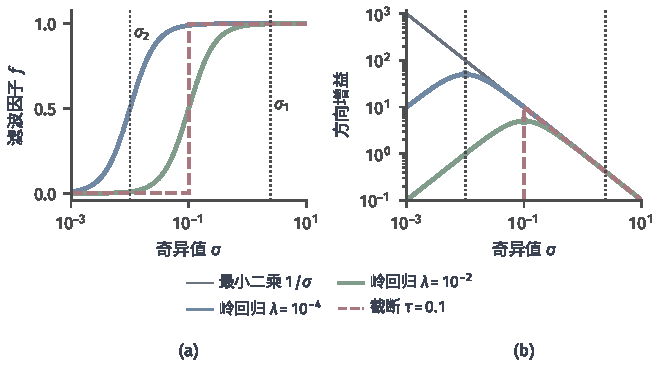
\includegraphics[width=112mm]{figures/01-basic-mathematics/03-vectors-matrices-and-multivariate-functions/matplotlib/c5-ridge-tsvd-filter-factors/figure.pdf}
 \caption{岭回归与截断SVD沿奇异方向的作用。(a)滤波因子：岭回归$f=\sigma^2/(\sigma^2+\lambda)$在$\sigma=\sqrt\lambda$处取$1/2$并连续过渡，截断SVD在阈值$\tau$处由$0$跳到$1$。(b)方向增益：最小二乘为$1/\sigma$，岭回归为$\sigma/(\sigma^2+\lambda)$，圆点是峰值$1/(2\sqrt\lambda)$；截断后小于$\tau$的方向增益为零。竖虚线是示例~\ref{ex:ls-tsvd-steps}中矩阵的两个奇异值。}
 \label{fig:ls-ridge-tsvd-filter-factors}
\end{figure}

\subsubsection{算法实现}
先区分两件事。第~\ref{sec:ls-qr-method}节的正交算法改善的是同一问题的计算过程；正则化则主动修改了问题，以控制敏感性。修改后的问题是增广最小二乘~\eqref{eq:ls-augmented-system}，所以首选的计算路线是对增广矩阵作QR分解，它适用于任意$\bm\Gamma$。下面写出这条路线的变量、输入与预处理和计算步骤，并在主要思想的小例子上执行。

\begin{example}[增广QR求岭回归]
\label{ex:ls-ridge-augmented-qr}
本例取主要思想中的教学例：
\[
 \bm A=\begin{bmatrix}3&0\\0&1\end{bmatrix},\qquad
 \bm b=\begin{bmatrix}3\\1\end{bmatrix},\qquad
 \bm\Gamma=\bm I,\qquad \lambda=1 .
\]
无惩罚时方程相容，解为$(1,1)^\top$。下面的逐步执行都在这个例子上进行。
\end{example}

\paragraph{变量}
\begin{itemize}
 \item $\tilde{\bm A}\in\mathbb R^{(m+p)\times d}$、$\tilde{\bm b}\in\mathbb R^{m+p}$：增广矩阵与增广右端。
 \item $\bm Q\in\mathbb R^{(m+p)\times d}$、$\bm R\in\mathbb R^{d\times d}$：$\tilde{\bm A}$的经济型QR因子，$\bm Q$的列标准正交，$\bm R$为对角元为正的上三角矩阵。
 \item $\bm g\in\mathbb R^d$：变换后的右端$\bm Q^\top\tilde{\bm b}$。
 \item $\bm x\in\mathbb R^d$：正则化解$\bm x_\lambda$。
 \item $\bm r\in\mathbb R^m$：原残差$\bm b-\bm A\bm x$；另报告惩罚量$\lVert\bm\Gamma\bm x\rVert_2$。
\end{itemize}

\paragraph{输入与预处理}
输入$\bm A,\bm b,\bm\Gamma,\lambda$。先核对$\bm A$与$\bm\Gamma$的列数相同、$\bm b$的长度等于$\bm A$的行数，再把增广矩阵与增广右端构造为
\[
 \tilde{\bm A}=\begin{bmatrix}\bm A\\ \sqrt\lambda\,\bm\Gamma\end{bmatrix},\qquad
 \tilde{\bm b}=\begin{bmatrix}\bm b\\ \bm0\end{bmatrix}.
\]
例中
\[
 \tilde{\bm A}=\begin{bmatrix}3&0\\0&1\\1&0\\0&1\end{bmatrix},\qquad
 \tilde{\bm b}=\begin{bmatrix}3\\1\\0\\0\end{bmatrix}.
\]

下面的步骤要求$\tilde{\bm A}$满列秩，即条件~\eqref{eq:linear-algebra-tikhonov-common-nullspace}成立；岭回归总满足这一条件。若条件不成立，增广问题的解不唯一，要先按第~\ref{chap:linear-solution-selection}章的准则另选代表，例如对$\tilde{\bm A}$作SVD取最小范数解。

\paragraph{计算步骤}
\begin{enumerate}
 \item \textbf{QR分解。}对$\tilde{\bm A}$作Householder QR（第~\ref{sec:ls-householder}节），得到
 \[
  \tilde{\bm A}=\bm Q\bm R .
 \]
 例中$\tilde{\bm A}$的两列$(3,0,1,0)^\top$与$(0,1,0,1)^\top$已经正交，长度分别为$\sqrt{10}$与$\sqrt2$，所以分解只需把两列单位化：
 \[
  \bm Q=\begin{bmatrix}3/\sqrt{10}&0\\0&1/\sqrt2\\1/\sqrt{10}&0\\0&1/\sqrt2\end{bmatrix},\qquad
  \bm R=\begin{bmatrix}\sqrt{10}&0\\0&\sqrt2\end{bmatrix}.
 \]

 \item \textbf{变换右端。}计算
 \[
  \bm g=\bm Q^\top\tilde{\bm b} .
 \]
 例中
 \[
  \bm g=\begin{bmatrix}9/\sqrt{10}\\1/\sqrt2\end{bmatrix}.
 \]

 \item \textbf{回代。}解上三角方程
 \[
  \bm R\bm x=\bm g .
 \]
 例中$\bm R$是对角的，两个分量分别为
 \[
  x_1=\frac{9/\sqrt{10}}{\sqrt{10}}=\frac9{10},\qquad
  x_2=\frac{1/\sqrt2}{\sqrt2}=\frac12 .
 \]

 \item \textbf{核验。}回到正则化目标，计算原残差与惩罚量，并检查增广正规残差
 \[
  \bm A^\top(\bm b-\bm A\bm x)-\lambda\bm\Gamma^\top\bm\Gamma\bm x
 \]
 接近零。例中
 \[
  \bm r=\bm b-\bm A\bm x=\begin{bmatrix}3-27/10\\1-1/2\end{bmatrix}=\begin{bmatrix}3/10\\1/2\end{bmatrix},
 \]
 惩罚量为
 \[
  \lVert\bm\Gamma\bm x\rVert_2=\sqrt{\frac{81}{100}+\frac14}\approx1.030 ,
 \]
 而
 \[
  \bm A^\top\bm r-\lambda\bm x=\begin{bmatrix}9/10-9/10\\1/2-1/2\end{bmatrix}=\bm0 ,
 \]
 增广正规条件成立。
\end{enumerate}

最终得到正则化解
\[
 \bm x_\lambda=\begin{bmatrix}9/10\\1/2\end{bmatrix},
\]
与主要思想中按滤波因子逐个方向算出的结果一致。原方程本来有精确解$(1,1)^\top$，算法得到的却是$(9/10,1/2)^\top$，残差不为零。这不是计算误差，而是新目标的解：惩罚项改变了要解的问题。

\paragraph{SVD路线}
$\bm\Gamma=\bm I$时还可以直接按式~\eqref{eq:matrix-analysis-ridge-filter-factor}计算。先作一次SVD，算出$c_i=\bm u_i^\top\bm b$；此后对每个$\lambda$，只需令
\[
 z_i=\frac{\sigma_ic_i}{\sigma_i^2+\lambda}\quad(i\leq r),\qquad \bm x_\lambda=\sum_{i=1}^rz_i\bm v_i .
\]
分解与$\lambda$无关，换一个参数只需重算$r$个系数与一次组合，所以要扫描多个参数时这条路线最省。

例中改取$\lambda=9$，滤波因子变为
\[
 f_1=\frac9{9+9}=\frac12,\qquad f_2=\frac1{1+9}=\frac1{10},
\]
立即得到$\bm x_\lambda=(1/2,1/10)^\top$，不必重新分解。

\paragraph{Cholesky路线}
也可以直接解定理~\ref{thm:ls-tikhonov-existence-uniqueness}中的方程：对$\bm A^\top\bm A+\lambda\bm\Gamma^\top\bm\Gamma$作Cholesky分解（第~\ref{sec:ls-cholesky}节），再依次前代、回代。推导中的这个正规矩阵并不是必须显式形成的对象；形成它会使条件数平方，下面的算法分析说明这条路线何时可靠。

\begin{example}[直线拟合的岭回归]
\label{ex:ls-ridge-line-fit}
沿用示例~\ref{ex:ls-line-least-squares}的直线拟合数据：
\[
 \bm A=\begin{bmatrix}1&0\\1&1\\1&2\end{bmatrix},\qquad
 \bm b=\begin{bmatrix}1\\2\\2\end{bmatrix},
\]
取$\bm\Gamma=\bm I$，$\lambda=1$，按Cholesky路线逐步计算。
\end{example}

\begin{enumerate}
 \item \textbf{形成方程。}由$\bm A^\top\bm A$加上$\lambda\bm I$与$\bm A^\top\bm b$，正则化后的方程为
 \[
  \begin{bmatrix}4&3\\3&6\end{bmatrix}\bm x=\begin{bmatrix}5\\6\end{bmatrix}.
 \]

 \item \textbf{Cholesky分解。}逐列计算
 \[
  \begin{gathered}
  l_{1,1}=\sqrt4=2,\qquad l_{2,1}=\frac32=1.5,\\
  l_{2,2}=\sqrt{6-1.5^2}=\frac{\sqrt{15}}2\approx1.9365 .
  \end{gathered}
 \]

 \item \textbf{前代。}
 \[
  y_1=\frac52=2.5,\qquad
  y_2=\frac{6-1.5\times2.5}{1.9365}=\frac{9}{2\sqrt{15}}\approx1.1619 .
 \]

 \item \textbf{回代。}
 \[
  x_2=\frac{1.1619}{1.9365}=0.6,\qquad
  x_1=\frac{2.5-1.5\times0.6}{2}=0.8 .
 \]

 \item \textbf{核验。}拟合值为$\bm A\bm x=(0.8,1.4,2.0)^\top$，残差为
 \[
  \bm r=\bm b-\bm A\bm x=\begin{bmatrix}0.2\\0.6\\0\end{bmatrix},\qquad
  \bm A^\top\bm r=\begin{bmatrix}0.8\\0.6\end{bmatrix}=\lambda\bm x ,
 \]
 正则化的正规残差$\bm A^\top\bm r-\lambda\bm x$为零。
\end{enumerate}

最终得到
\[
 \bm x_\lambda=\begin{bmatrix}0.8\\0.6\end{bmatrix}.
\]
与最小二乘解$(7/6,1/2)^\top$相比，残差平方由$1/6$增至$0.4$，解的长度由$1.269$降为$1$。

按SVD路线核对：$\sigma_1^2\approx7.162$，$\sigma_2^2\approx0.838$，滤波因子为$f_1\approx0.877$、$f_2\approx0.456$。$\sigma_2^2$与$\lambda$相当，第二个方向被压掉约一半。

\paragraph{大型问题}
$\bm A$很大且只能通过乘向量访问时，可以把LSQR（第~\ref{sec:ls-lsqr}节）用于增广问题~\eqref{eq:ls-augmented-system}：$\tilde{\bm A}$乘向量只需分别乘$\bm A$与$\bm\Gamma$，不必形成增广矩阵。

\subsubsection{算法分析}

\paragraph{正确性}
由定理~\ref{thm:ls-tikhonov-existence-uniqueness}，正则化目标的极小点就是增广问题~\eqref{eq:ls-augmented-system}的最小二乘解。条件~\eqref{eq:linear-algebra-tikhonov-common-nullspace}成立时$\tilde{\bm A}$满列秩，$\bm R$可逆，增广QR回代得到的就是这个唯一解；三条路线解的是同一个问题，在精确算术下给出同一个$\bm x_\lambda$。

\paragraph{数值敏感度}
增广QR对$\tilde{\bm A}$作正交变换，误差由$\kappa_2(\tilde{\bm A})$控制；Cholesky路线分解的是$\tilde{\bm A}^\top\tilde{\bm A}$，条件数是$\kappa_2(\tilde{\bm A})^2$。岭回归中$\tilde{\bm A}^\top\tilde{\bm A}$的特征值为$\sigma_i^2+\lambda$，所以
\begin{equation}
 \kappa_2(\tilde{\bm A})=\Bigl(\frac{\sigma_1^2+\lambda}{\sigma_d^2+\lambda}\Bigr)^{1/2}\leq\Bigl(1+\frac{\sigma_1^2}{\lambda}\Bigr)^{1/2},
 \label{eq:ls-ridge-augmented-condition}
\end{equation}
其中$\sigma_d$为第$d$个奇异值，秩亏时为零。这个界不依赖最小奇异值，即使$\bm A$秩亏也有界。所以只在$\lambda$不太小、$(1+\sigma_1^2/\lambda)u\ll1$时，Cholesky路线与增广QR同样可靠。

直线拟合例中$\kappa_2(\bm A)^2\approx8.55$，正则化后$\kappa_2(\tilde{\bm A})^2\approx4.44$：惩罚本身就改善了条件。

\paragraph{结果检验}
无论哪条路线，结果都要回到正则化目标核验：分别报告拟合误差$\lVert\bm A\bm x_\lambda-\bm b\rVert_2$与惩罚大小$\lVert\bm\Gamma\bm x_\lambda\rVert_2$，正规残差应检查$\bm A^\top(\bm b-\bm A\bm x_\lambda)-\lambda\bm\Gamma^\top\bm\Gamma\bm x_\lambda$，而不是原问题的$\bm A^\top\bm r$。

增广QR例中两者分别约为$0.583$与$1.030$；那里$\bm A^\top\bm r=(9/10,1/2)^\top$并不为零，用原问题的标准检查会误判为没有收敛。

\paragraph{计算代价}
增广QR处理$(m+p)\times d$的矩阵，稠密时代价为$O((m+p)d^2)$。Cholesky路线形成正规矩阵约需$md^2$次运算，分解约需$d^3/3$次，与第~\ref{sec:ls-normal-equations-method}节正规方程法的代价相同。SVD路线的一次分解为$O(md^2)$，此后每个新的$\lambda$只需$O(rd)$次运算。

\subsection{谱截断正则化}
\label{sec:ls-tsvd-solve}

\subsubsection{主要思想}

\paragraph{最小范数解中的放大}
从第~\ref{chap:singular-value-decomposition}章的SVD出发，先在奇异坐标中写出最小范数最小二乘解：
\[
 \bm A^\dagger\bm b=\sum_{i=1}^r\frac{c_i}{\sigma_i}\,\bm v_i ,\qquad c_i=\bm u_i^\top\bm b .
\]
右端在第$i$个左奇异方向上的误差进入$c_i$，再被放大$1/\sigma_i$倍。若误差预算表明某些方向的观测分量$c_i$主要是噪声，就不应在这些方向上反演。谱截断正则化因此只在可靠的奇异方向上恢复系数。

\paragraph{只保留可靠方向}
给定阈值$\tau$，取保留集$J=\{i:\sigma_i>\tau\}$；也可以事先指定保留最大的$k$个正奇异值。奇异值按降序排列，所以$J=\{1,\ldots,k\}$，$k=|J|$。令
\begin{equation}
 \bm x_k=\sum_{i=1}^k\frac{c_i}{\sigma_i}\,\bm v_i ,\qquad 1\leq k\leq r .
 \label{eq:ls-tsvd-solution}
\end{equation}
这种做法称为\term{截断SVD}（truncated SVD）求解。与岭回归的式~\eqref{eq:matrix-analysis-ridge-filter-factor}对照，它相当于把滤波因子取为$f_i=1$（$i\leq k$）或$f_i=0$（$i>k$）。

\begin{example}[对角矩阵的谱截断]
\label{ex:ls-tsvd-diagonal}
取$\bm A=\operatorname{diag}(1,1/100)$，真实系数$\bm x_{\mathrm{true}}=(1,1)^\top$，无噪声的观测为$(1,1/100)^\top$。设第二个观测带误差$2/100$，实际得到
\[
 \bm b=\begin{bmatrix}1\\3/100\end{bmatrix}.
\]
这里$\sigma_1=1$，$\sigma_2=1/100$，奇异向量就是坐标向量，$c_1=1$，$c_2=3/100$。按分量写出不截断时的系数、取$\tau=1/10$时的滤波因子与截断后的系数：
\[
 \begin{aligned}
 &\text{第一个方向：}&& \frac{c_1}{\sigma_1}=1,\qquad f_1=1,\qquad f_1\frac{c_1}{\sigma_1}=1;\\
 &\text{第二个方向：}&& \frac{c_2}{\sigma_2}=3,\qquad f_2=0,\qquad f_2\frac{c_2}{\sigma_2}=0 .
 \end{aligned}
\]
不截断时得到$(1,3)^\top$：第二个方向把误差$2/100$放大了一百倍。截断只保留$\sigma_1$，得到
\[
 \bm x_1=\begin{bmatrix}1\\0\end{bmatrix}.
\]

两种恢复的误差范数分别为
\[
 \lVert(1,3)^\top-(1,1)^\top\rVert_2=2,\qquad \lVert(1,0)^\top-(1,1)^\top\rVert_2=1,
\]
截断的误差较小。

但这个改善是以丢掉真实的第二分量为代价的：若真值的第二分量很大而噪声很小，截断反而更差。不能从一个算例推断任意真值和噪声下截断都更好，算法分析中的误差分解说明了一般情形。
\end{example}

\paragraph{限制子空间上的最小二乘}
截断解并非随意拼出的近似，它是一个限制在子空间上的最小二乘解。把系数限制在$\operatorname{span}\{\bm v_1,\ldots,\bm v_k\}$中，写$\bm x=\sum_{i\leq k}z_i\bm v_i$，则$\bm A\bm x=\sum_{i\leq k}\sigma_iz_i\bm u_i$。把$\bm b$按左奇异方向与列空间的正交补分开，残差平方分成三部分：
\begin{equation}
 \begin{aligned}
 \lVert\bm A\bm x-\bm b\rVert_2^2
 &=\sum_{i=1}^k(\sigma_iz_i-c_i)^2+\sum_{i=k+1}^rc_i^2\\
 &\quad+\lVert(\bm I-\bm A\bm A^\dagger)\bm b\rVert_2^2 .
 \end{aligned}
 \label{eq:ls-tsvd-restricted-residual}
\end{equation}
只有第一项依赖$\bm z$，取$z_i=c_i/\sigma_i$使它为零，就得到$\bm x_k$。被舍弃方向上的观测分量$c_{k+1},\ldots,c_r$无法再被拟合，全部转入残差。对角例中残差为
\[
 \bm b-\bm A\bm x_1=\begin{bmatrix}0\\3/100\end{bmatrix},
\]
正是被舍弃的观测分量$c_2$。

\paragraph{与截断矩阵的关系}
用矩阵写，令
\begin{equation}
 \bm A_k=\sum_{i=1}^k\sigma_i\bm u_i\bm v_i^\top ,
 \label{eq:ls-truncated-matrix}
\end{equation}
即只保留前$k$项的SVD，则$\bm x_k=\bm A_k^\dagger\bm b$，是以$\bm A_k$代替$\bm A$后的最小范数最小二乘解。第~\ref{chap:matrix-approximation}章将把$\bm A_k$作为矩阵的低秩逼近来研究。两者共用同一个分解，目的却不同：低秩逼近要重建矩阵，截断求解要从带误差的观测中稳定地恢复输入。

\subsubsection{算法实现}
算法先求SVD并把右端投影到左奇异方向，再按保留规则逐个方向设置系数，最后合成解并读出残差。下面写出计算中用到的变量、输入与预处理和计算步骤，并在一个近共线的设计上执行。

\begin{example}[近共线设计的截断求解]
\label{ex:ls-tsvd-steps}
设计矩阵与观测为
\[
 \bm A=\begin{bmatrix}1&1\\1&1.01\\1&0.99\end{bmatrix},\qquad
 \bm b=\begin{bmatrix}1\\1.1\\0.9\end{bmatrix}.
\]
这是示例~\ref{ex:ls-nearly-collinear-design}中取$\bm c=(1,1,1)^\top$、$\bm q=(0,1,-1)^\top$、$\varepsilon=0.01$、$\delta=0.1$的情形。阈值取$\tau=0.1$。
\end{example}

\paragraph{变量}
\begin{itemize}
 \item $\sigma_i,\bm u_i,\bm v_i$（$i\leq r$）：经济型SVD的正奇异值与奇异向量，奇异值按降序排列。
 \item $\bm c\in\mathbb R^r$：右端在左奇异方向上的分量$c_i=\bm u_i^\top\bm b$。
 \item $J$与$k=|J|$：保留集与保留的方向数。
 \item $\bm z\in\mathbb R^r$：解在右奇异方向上的系数。
 \item $\bm x\in\mathbb R^d$：截断解$\bm x_k$。
 \item $\bm r\in\mathbb R^m$：原残差$\bm b-\bm A\bm x$。
\end{itemize}

\paragraph{输入与预处理}
输入$\bm A,\bm b$与阈值$\tau$（或保留数$k$），求$\bm A$的经济型SVD。例中
\[
 \sigma_1\approx2.4495,\qquad \sigma_2\approx0.0100,
\]
右奇异向量为
\[
 \bm v_1\approx\frac1{\sqrt2}\begin{bmatrix}1\\1\end{bmatrix},\qquad
 \bm v_2\approx\frac1{\sqrt2}\begin{bmatrix}1\\-1\end{bmatrix},
\]
左奇异向量为
\[
 \bm u_1\approx\begin{bmatrix}0.5773\\0.5802\\0.5745\end{bmatrix},\qquad
 \bm u_2\approx\begin{bmatrix}0.0024\\-0.7047\\0.7095\end{bmatrix}.
\]

\paragraph{计算步骤}
\begin{enumerate}
 \item \textbf{投影右端。}计算
 \[
  \bm c=\bm U^\top\bm b .
 \]
 例中
 \[
  c_1\approx1.7326,\qquad c_2\approx-0.1343 .
 \]

 \item \textbf{确定保留集。}取$J=\{i:\sigma_i>\tau\}$，$k=|J|$。例中只有$\sigma_1$超过阈值$0.1$，所以
 \[
  J=\{1\},\qquad k=1 .
 \]

 \item \textbf{设置系数。}逐项令
 \begin{equation}
  z_i=\begin{cases}c_i/\sigma_i,& i\in J,\\ 0,& i\notin J .\end{cases}
  \label{eq:ls-tsvd-coefficients}
 \end{equation}
 所有除法只在保留的正奇异值上执行。例中
 \[
  z_1=\frac{1.7326}{2.4495}\approx0.7073,\qquad z_2=0 .
 \]
 若不截断，第二个系数将是$c_2/\sigma_2\approx-13.435$。

 \item \textbf{合成解。}计算
 \[
  \bm x=\sum_{i\in J}z_i\bm v_i .
 \]
 例中
 \[
  \bm x_1\approx0.7073\,\bm v_1\approx\begin{bmatrix}0.5001\\0.5002\end{bmatrix}.
 \]

 \item \textbf{读出拟合值与残差。}由$\bm A\bm v_i=\sigma_i\bm u_i$，拟合值是
 \begin{equation}
  \bm A\bm x_k=\sum_{i\in J}c_i\bm u_i ,
  \label{eq:ls-tsvd-fitted-values}
 \end{equation}
 不必再乘$\bm A$。残差由被舍弃方向的分量与列空间外的部分组成。例中$\bm b$在$\bm A$的列空间内（$\lVert\bm b\rVert_2^2=c_1^2+c_2^2$），残差全部来自被舍弃的第二个方向：
 \[
  \bm r=c_2\bm u_2\approx\begin{bmatrix}-0.0003\\0.0947\\-0.0953\end{bmatrix},\qquad
  \lVert\bm r\rVert_2=|c_2|\approx0.1343 .
 \]

 \item \textbf{核验。}检查原残差，并检查限制子空间中的正规条件
 \begin{equation}
  \bm v_i^\top\bm A^\top\bm r=0\qquad(i\in J).
  \label{eq:ls-tsvd-restricted-normal-condition}
 \end{equation}
 例中$\bm v_1^\top\bm A^\top\bm r=\sigma_1\bm u_1^\top\bm r=0$成立；完整的正规残差却是
 \[
  \bm A^\top\bm r=\sigma_2c_2\bm v_2\approx\begin{bmatrix}-0.00095\\0.00095\end{bmatrix},
 \]
 长度约为$0.0013$，不为零：$\bm x_1$不是原问题的最小二乘解。
\end{enumerate}

最终得到截断解
\[
 \bm x_1\approx\begin{bmatrix}0.50\\0.50\end{bmatrix}.
\]
换一个阈值只需增减和式中的项。若取$\tau<\sigma_2$，第二个方向贡献$(c_2/\sigma_2)\bm v_2\approx-13.4\,\bm v_2$，解变为精确拟合的$(-9,10)^\top$，与示例~\ref{ex:ls-nearly-collinear-design}的最小二乘解相同。

两者对照，截断以约$0.134$的残差为代价，把一对此增彼减的大系数换成了两个接近$0.5$的系数。

\subsubsection{算法分析}

\paragraph{误差分解}
设观测由真实输入加噪声得到。截断解的误差与拟合损失都可以按奇异方向分开。

\begin{theorem}[截断SVD的误差分解]
\label{thm:ls-tsvd-error-decomposition}
设$\bm b=\bm A\bm x_{\mathrm{true}}+\bm e$，$\bm x_{\mathrm{true}}\in\operatorname{range}\bm A^\top$，$1\leq k\leq r$。则
\begin{equation}
 \begin{aligned}
 \bm x_k-\bm x_{\mathrm{true}}
 &=\sum_{i=1}^k\frac{\bm u_i^\top\bm e}{\sigma_i}\,\bm v_i\\
 &\quad-\sum_{i=k+1}^r(\bm v_i^\top\bm x_{\mathrm{true}})\,\bm v_i ,
 \end{aligned}
 \label{eq:ls-tsvd-error-decomposition}
\end{equation}
两项正交，第一项的长度不超过$\lVert\bm e\rVert_2/\sigma_k$。此外
\begin{equation}
 \begin{gathered}
 \lVert\bm b-\bm A\bm x_k\rVert_2^2=\lVert\bm b-\bm A\hat{\bm x}\rVert_2^2+\sum_{i=k+1}^rc_i^2,\\
 \bm A^\top(\bm b-\bm A\bm x_k)=\sum_{i=k+1}^r\sigma_ic_i\bm v_i ,
 \end{gathered}
 \label{eq:ls-tsvd-residual-decomposition}
\end{equation}
其中$\hat{\bm x}$为任一最小二乘解。
\end{theorem}
\begin{proof}
由$c_i=\sigma_i\bm v_i^\top\bm x_{\mathrm{true}}+\bm u_i^\top\bm e$，
\[
 \bm x_k=\sum_{i\leq k}\Bigl(\bm v_i^\top\bm x_{\mathrm{true}}+\frac{\bm u_i^\top\bm e}{\sigma_i}\Bigr)\bm v_i .
\]
而$\bm x_{\mathrm{true}}=\sum_{i\leq r}(\bm v_i^\top\bm x_{\mathrm{true}})\bm v_i$，相减即得误差式。两项落在互相正交的$\bm v_i$上；第一项长度的平方为
\[
 \sum_{i\leq k}\frac{(\bm u_i^\top\bm e)^2}{\sigma_i^2}\leq\frac{\lVert\bm e\rVert_2^2}{\sigma_k^2}.
\]

再看残差。由$\bm A\bm x_k=\sum_{i\leq k}c_i\bm u_i$，
\[
 \bm b-\bm A\bm x_k=(\bm I-\bm A\bm A^\dagger)\bm b+\sum_{i>k}c_i\bm u_i ,
\]
两部分正交，前者就是最小二乘残差；再用$\bm A^\top\bm u_i=\sigma_i\bm v_i$与$\bm A^\top(\bm I-\bm A\bm A^\dagger)=\bm0$得正规残差。
\end{proof}

第一项是保留方向的噪声放大，它的界由$\sigma_k$而不是$\sigma_r$决定；第二项是舍弃方向上真实输入的全部损失，这就是截断引入的偏差。在例~\ref{ex:ls-tsvd-diagonal}中，不截断（$k=r$）时没有舍弃项，误差$(0,2)^\top$全部是噪声放大；截断后误差$(0,-1)^\top$全部是偏差。

拟合的代价是残差平方多出被舍弃的$c_i^2$。正规残差只落在被舍弃的方向上，所以限制子空间中的正规条件成立，而完整的正规条件一般不成立；近共线例中正规残差$\sigma_2c_2\bm v_2$的长度约为$0.0013$，正是这一项。

\paragraph{计算代价}
主要计算代价是一次SVD，稠密时为$O(md^2)$量级。分解完成后，投影右端约需$mr$次运算，合成解约需$dk$次；换阈值或换保留数不必重新分解。

\subsubsection{与岭回归的比较}
岭回归连续地压低小奇异值方向，截断则把滤波因子直接取成$1$（$i\leq k$）或$0$（$i>k$），两者在图~\ref{fig:ls-ridge-tsvd-filter-factors}中分别是光滑曲线与阶梯。要看出这种差别对结果的影响，最直接的办法是在同一组数据上比较两者的解、残差，以及观测改动后解的变化。

\begin{example}[岭回归与截断SVD的比较]
\label{ex:ls-regularization-response}
沿用示例~\ref{ex:ls-tsvd-steps}的数据，再把$\bm b$改为$(1,1.11,0.89)^\top$，这个扰动几乎全部落在$\bm u_2$上。下表前两列是原观测下各方法的解与残差长度，最后一列是改动观测后系数的变化与观测的变化之比：
\[
 \begin{array}{lccc}
  \text{方法} & \bm x & \lVert\bm r\rVert_2 & \lVert\Delta\bm x\rVert_2/\lVert\Delta\bm b\rVert_2\\[2pt]
  \text{最小二乘} & (-9,\,10)^\top & 0 & 100\\
  \lambda=10^{-4} & (-4.25,\,5.25)^\top & 0.067 & 50\\
  \lambda=10^{-2} & (0.41,\,0.59)^\top & 0.133 & 0.99\\
  k=1 & (0.50,\,0.50)^\top & 0.134 & 0.002
 \end{array}
\]
响应比就是第二个方向的增益：最小二乘为$1/\sigma_2=100$，岭回归为$\sigma_2/(\sigma_2^2+\lambda)$，截断后为零，剩下的$0.002$来自扰动在$\bm u_1$上的微小分量。
\end{example}

表中可以读出两点。第一，精确拟合的大系数全部来自第二个方向，系数越稳定，残差越大。第二，$\lambda=10^{-2}$的岭回归与$k=1$的截断已经很接近：这时$f_2\approx0.0099$，岭回归几乎也把第二个方向舍去了。

两种方法适用的场景不同。奇异值在某处明显下降时，截断位置有自然的选择，截断把可信与不可信的方向分得最清楚；奇异值缓慢衰减、没有明显间隔时，连续衰减的岭回归更平稳。

阈值应联系噪声规模、截断处的奇异值间隔和任务目标。取$\tau$为数据误差的估计，就是只在第~\ref{sec:ls-pseudoinverse-rank-change}节意义下可辨认的方向上反演；它不等同于按机器精度判定精确秩，只有数据仅含舍入误差时两者才一致。

\subsubsection{与低秩逼近的边界}
截断求解与矩阵的低秩逼近共用$\bm A_k$，但两者的最优性不能互相借用。第~\ref{chap:matrix-approximation}章将证明，$\bm A_k$在谱范数与Frobenius范数下是最佳秩$k$重建（定理~\ref{thm:matrix-analysis-best-low-rank}）。这一结论只说$\bm A_k$离$\bm A$最近，不说$\bm x_k$拟合得最好：由定理~\ref{thm:ls-tsvd-error-decomposition}的正规残差，除非被舍弃的$c_i$全为零，$\bm x_k$不是原问题的最小二乘解。矩阵逼近的最优性也不涉及$\bm x_{\mathrm{true}}$与$\bm e$，更不能由它断言$\bm x_k$最接近未知的真实输入。

所以截断求解要同时说明保留了哪些方向、噪声水平多大、允许多大的拟合损失。保留的方向本身是否可靠，还要看截断处的间隔$\sigma_k-\sigma_{k+1}$：间隔很小时，扰动可能使前$k$个奇异方向明显偏转，第~\ref{sec:ls-subspace-sensitivity}节的奇异值与子空间扰动界可以用来判断。

\section{求解方法的比较与选择}
\label{sec:ls-method-selection}

第~\ref{chap:direct-linear-solvers}—\ref{chap:row-projection-methods}章分别给出了直接分解、最小二乘的直接求解、定常迭代、Krylov子空间法与行列投影法。每一章都在自己的前提下说明了方法怎样计算、何时成立，但没有把不同章的方法放在同一个问题上比较。本节做这件事。

比较之前，先要确定比较什么。同一个矩阵上，两种方法可能求的根本不是同一个解；即使求同一个解，一种方法也可能要求另一种方法不需要的矩阵性质。所以本节按四个维度依次比较，每个维度回答一个问题。

第一个维度是求解目标：要的是精确解、最小二乘解还是最小范数解，以及方法能否直接面对这个目标。第二个维度是矩阵条件：方法对矩阵的形状、对称性、正定性和秩有什么要求，需要怎样访问矩阵。第三个维度是计算开销与收敛速度：达到同一精度一共要付出多少运算、存储和数据读取。第四个维度是数值稳定性：有限精度下结果的误差来自哪里，算法本身会不会额外放大误差。最后把四个维度合起来，给出几类典型问题的取舍。

比较的对象始终是“达到相同要求的总成本”。第~\ref{sec:ls-truncated-svd-ridge}节的正则化与谱截断不在此列：它们改变了求解目标，得到的系数较小、计算也可能更便宜，但这不表示把原问题解得更准确，不能与求原问题的方法按成本或误差直接比较。

\subsection{求解目标与方法适用性}
\label{sec:ls-method-selection-goals}

\paragraph{三种验收要求}
第~\ref{chap:linear-solution-selection}章区分了三种求解目标。它们在多数情况下不同，因此检验一个结果是否合格的标准也不同。

相容方程$\bm A\bm x=\bm b$要求原残差为零；一般最小二乘问题$\min_{\bm x}\lVert\bm A\bm x-\bm b\rVert_2$只要求残差与列空间正交；最小范数解在此之上还要求解不含$\ker\bm A$的分量（第~\ref{sec:ls-select-among-solutions}节）。记$\bm r=\bm b-\bm A\bm x$，三种要求依次为
\begin{equation}
 \bm r=\bm0;\qquad
 \bm A^\top\bm r=\bm0;\qquad
 \bm A^\top\bm r=\bm0\ \text{且}\ \bm x\in\operatorname{range}\bm A^\top .
 \label{eq:ls-method-selection-acceptance}
\end{equation}

方程相容时，前两种要求给出同一个解集。方程不相容时，最优残差停在一个正的长度上，第一种要求无法满足。以第~\ref{sec:ls-lsqr}节的不相容系统为例：
\[
 \bm A=\begin{bmatrix}1&0\\0&2\\0&0\end{bmatrix},\qquad
 \bm b=\begin{bmatrix}1\\1\\1\end{bmatrix}.
\]
它的最小二乘解与最优残差为
\[
 \hat{\bm x}=\begin{bmatrix}1\\1/2\end{bmatrix},\qquad
 \hat{\bm r}=\begin{bmatrix}0\\0\\1\end{bmatrix}.
\]
这里$\lVert\hat{\bm r}\rVert_2=1$，而$\bm A^\top\hat{\bm r}=\bm0$，$\hat{\bm x}$已经是最小二乘解。若按原残差趋于零来判断，任何方法在这个问题上都不会“成功”。所以不能把所有算法都按$\lVert\bm r\rVert_2\to0$检验。

第三种要求在解不唯一时才起作用。例~\ref{ex:ls-qr-min-norm-run}的方程为
\[
 \begin{bmatrix}1&0&1\\0&1&1\end{bmatrix}\bm x=\begin{bmatrix}1\\2\end{bmatrix}.
\]
它有无穷多解，$(0,1,1)^\top$与$(1,2,0)^\top$的残差都为零，但前者与$\ker\bm A$的方向$(1,1,-1)^\top$正交，范数为$\sqrt2$；后者含零空间分量，范数为$\sqrt5$。残差检验分不出两者，只有第三种要求能把最小范数解挑出来。

\paragraph{经正规方程转换}
求解目标与方法要求的输入不一致时，可以先改写问题。最常见的改写是正规方程。满列秩时，最小二乘解是
\[
 \bm A^\top\bm A\bm x=\bm A^\top\bm b
\]
的唯一解，系数矩阵$\bm A^\top\bm A$对称正定。于是长方的最小二乘问题变成一个对称正定方程，可以交给Cholesky分解、CG或在对称正定矩阵上收敛的定常迭代。

这种改写有三项代价。其一，显式形成$\bm A^\top\bm A$时，稀疏矩阵可能变稠密：$\bm A$只要有一行全是非零元，这一行的外积就填满整个Gram矩阵。

其二，条件数变为平方（式~\eqref{eq:matrix-analysis-normal-equation-condition-square}），
\[
 \kappa_2(\bm A^\top\bm A)=\kappa_2(\bm A)^2 .
\]
例~\ref{ex:ls-rhs-perturbation-near-parallel}的$\bm A_2$取$\varepsilon=10^{-8}$时，$\kappa_2(\bm A_2)\approx2\times10^8$，双精度下两列仍可区分；但Gram矩阵的元素$1+\varepsilon^2$舍入后就是$1$，存下来的$\bm A_2^\top\bm A_2$已经奇异（第~\ref{sec:ls-ls-regularization-sensitivity}节）。

其三，不显式形成$\bm A^\top\bm A$时，迭代法每次作用它仍要一次$\bm A$乘向量和一次$\bm A^\top$乘向量。此外，秩亏时$\bm A^\top\bm A$只是半正定，正定矩阵上的唯一性与收敛保证都不能照搬。

\paragraph{经增广方程转换}
另一种改写不消去残差，而把它也当作未知量：残差的定义$\bm r+\bm A\bm x=\bm b$与正交条件$\bm A^\top\bm r=\bm0$合起来，是一个关于$(\bm r,\bm x)$的方阵方程。下面的定理说明这个方程的性质，它决定了能用哪些方法求解。

\begin{theorem}[最小二乘的增广方程]
\label{thm:ls-augmented-kkt-system}
设$\bm A\in\mathbb R^{m\times d}$满列秩，则方程
\begin{equation}
 \begin{bmatrix}\bm I_m&\bm A\\ \bm A^\top&\bm0\end{bmatrix}
 \begin{bmatrix}\bm r\\ \bm x\end{bmatrix}
 =\begin{bmatrix}\bm b\\ \bm0\end{bmatrix}
 \label{eq:ls-augmented-kkt-system}
\end{equation}
有唯一解，$\bm x$为最小二乘解，$\bm r$为相应残差；其系数矩阵对称、可逆且不定。
\end{theorem}
\begin{proof}
第一块行给出$\bm r=\bm b-\bm A\bm x$，第二块行就是正规方程$\bm A^\top(\bm b-\bm A\bm x)=\bm0$，所以解与最小二乘解一一对应。对称性显然。

若系数矩阵作用于$(\bm r;\bm x)$得零，则$\bm r=-\bm A\bm x$且$\bm A^\top\bm A\bm x=\bm0$，满列秩时只能$\bm x=\bm0$、$\bm r=\bm0$，故可逆。

再看不定性。取$(\bm u;\bm0)$，$\bm u\ne\bm0$，二次型为$\lVert\bm u\rVert_2^2>0$；取$(-\bm A\bm x;\bm x)$，$\bm x\ne\bm0$，二次型为$-\lVert\bm A\bm x\rVert_2^2<0$，故不定。
\end{proof}

在上面的不相容例子中，$\bm A$的两列分别只在第一、二行非零。按$(r_1,x_1)$、$(r_2,x_2)$、$r_3$重排未知量后，$5$阶增广矩阵分解为三个对角块：
\[
 \begin{bmatrix}1&1\\1&0\end{bmatrix},\qquad
 \begin{bmatrix}1&2\\2&0\end{bmatrix},\qquad
 \begin{bmatrix}1\end{bmatrix}.
\]
二阶块$\left[\begin{smallmatrix}1&\sigma\\\sigma&0\end{smallmatrix}\right]$的特征值是$(1\pm\sqrt{1+4\sigma^2})/2$，所以增广矩阵的五个特征值约为
\[
 1.618,\quad -0.618,\quad 2.562,\quad -1.562,\quad 1,
\]
正负都有，确实不定。解出的$(\bm r;\bm x)=(0,0,1;\,1,1/2)$正是前面的最优残差与最小二乘解。

因此，满列秩最小二乘也可以用分块$\mathrm{LDL}^\top$分解（第~\ref{sec:ls-ldlt}节）或MINRES（第~\ref{sec:ls-minres}节）求解，而不能用要求正定的Cholesky或CG。与正规方程相比，这一改写保留了$\bm A$的稀疏结构，也不使条件数平方；代价是未知量从$d$个增加到$m+d$个，存储与预条件都要按新的分块结构设计。

\paragraph{三种适用方式}
有了这两种改写，方法与目标的关系可以分成三种，下文统一使用这三种说法。

“直接适用”指方法直接以原问题的目标和数据为输入，例如QR、SVD与LSQR直接处理矩形最小二乘。“需转换”指先改变方程的表示，例如经正规方程或增广方程变成方阵方程，再交给方阵方法。“需扩展版本”指要修改算法本身，才能处理秩亏、不相容或最小范数的要求，例如扩展Kaczmarz相对于标准Kaczmarz。

三种方式都只说明方法能够面对这个目标，不说明它一定收敛。能对转换后的方程写出迭代公式，并不等于转换后的矩阵满足这种迭代的收敛条件。

\subsection{矩阵条件}
\label{sec:ls-method-selection-matrix}

目标确定以后再看矩阵。每种方法的正确性与收敛性都建立在一组矩阵条件之上：形状是方阵还是长方，是否对称、正定，秩是否完全。除此之外，方法还规定了它怎样读取矩阵：有的要把矩阵存下来做分解，有的只要计算矩阵乘向量，有的还要转置乘向量，有的每次只读一行。实际问题能提供哪种访问方式，常常与矩阵的数学性质一样限制方法的选择。

下面按章分组说明，最后用表~\ref{tab:ls-method-applicability}汇总。表中的迭代法都按第~\ref{chap:stationary-iterations}—\ref{chap:row-projection-methods}章建立的基本版本比较，某一行的限制不能推广到同名算法的所有扩展。

\paragraph{方阵的直接分解}
第~\ref{chap:direct-linear-solvers}章的方法都要求矩阵非奇异，并且要能存下矩阵和因子。带部分选主元的LU分解对任何非奇异方阵都能进行。Cholesky分解要求对称正定，这一条件既是充分的也是必要的，运算量是LU的一半。分块$\mathrm{LDL}^\top$分解只要求对称非奇异，允许不定，负主元与二阶块保留在$\bm D$中。低秩更新不是独立的分解，它要求修改前的矩阵已经分解、修改的秩很低，并且辅助矩阵可逆；它节省的是重新分解的工作。

这些方法都以方阵方程为对象，用于不相容最小二乘时须先转换：Cholesky用于满列秩的正规方程，分块$\mathrm{LDL}^\top$用于增广方程。普通LU直接作用于长方矩阵时并不保留最小二乘的目标。

\paragraph{最小二乘的直接求解}
第~\ref{chap:direct-least-squares-solvers}章的三条路线直接以最小二乘为目标，区别在于对秩的要求。正规方程法要求满列秩，并承受条件数平方。QR求解在满列秩时回代得到唯一最小二乘解，在满行秩时对$\bm A^\top$分解得到最小范数解；秩亏时$\bm R$出现零对角元，基本QR不能直接给出最小范数解。SVD求解对任意形状和秩都给出$\bm A^\dagger\bm b$，代价是分解更贵，小奇异值处的误差放大也要另行处理。三条路线都需要显式存储$\bm A$；正规方程法还可以按行累计Gram矩阵，适合观测逐批到达的情形。

\paragraph{定常迭代}
第~\ref{chap:stationary-iterations}章的方法求解可逆方阵方程，收敛当且仅当迭代矩阵的谱半径小于一：
\[
 \rho(\bm I-\bm M^{-1}\bm A)<1 .
\]
各方法的区别在于有哪些条件能保证这一点。Richardson只需矩阵乘向量；对称正定时收敛当且仅当$0<\alpha<2/\lambda_{\max}$。Jacobi与Gauss--Seidel要求对角元非零，这只保证可以执行；严格行对角占优对两者都保证收敛，对称正定只保证Gauss--Seidel收敛，不保证Jacobi收敛。SOR在对称正定矩阵上收敛当且仅当$0<\omega<2$。SSOR要求对称正定与$0<\omega<2$，每轮做前向与反向两次扫掠。

定常迭代用于最小二乘时须经正规方程转换。满列秩时$\bm A^\top\bm A$对称正定，Gauss--Seidel、SOR与SSOR的收敛保证随之成立，Jacobi仍须另行检查。在贯穿例~\ref{ex:ls-stationary-running-example}的$\bm A=\left[\begin{smallmatrix}4&1\\1&3\end{smallmatrix}\right]$上，五种方法都收敛，但谱半径各不相同，这在下一小节比较。

\paragraph{Krylov子空间法}
第~\ref{chap:krylov-methods}章的求解器按矩阵类型分工。CG要求对称正定。MINRES要求对称非奇异，允许不定；用于奇异对称矩阵时，判断是否到达最小二乘解要看$\lVert\bm A\bm r_k\rVert_2$，所得的解一般也不是最小范数解。GMRES、BiCG与BiCGSTAB适用于一般非奇异方阵，不要求对称。

这几种方法对矩阵访问的要求不同。CG、MINRES、GMRES与BiCGSTAB只需计算$\bm A\bm v$；BiCG还需计算$\bm A^\top\bm u$，转置作用难以获得时就不能使用。它们都是方阵方法，用于不相容最小二乘须先转换：CG可用于满列秩的正规方程，MINRES可用于增广方程。

LSQR与LSMR是第~\ref{chap:krylov-methods}章中直接处理长方矩阵的两种迭代法。它们允许长方、秩亏和不相容，每轮需要$\bm A\bm v$与$\bm A^\top\bm u$各一次，零初值时选出最小范数解。两者也能求解相容方程。

\paragraph{行列投影法}
第~\ref{chap:row-projection-methods}章的方法每次只读一行或一列。标准Kaczmarz求解相容方程，零初值时收敛到最小范数解；方程不相容时，它在各行的解之间往返，不论循环还是随机选行，都不会停在最小二乘解上。扩展Kaczmarz用列投影逐步分离出右端中不可拟合的部分，再对校正后的相容方程作行投影，因此能求最小范数最小二乘解，代价是还要能按列访问矩阵。

\paragraph{汇总}
表~\ref{tab:ls-method-applicability}汇总了上面的条件。表中“需转换”时，要对转换后的系统重新检查结构、条件数、零空间与误差度量；标为“直接适用”也不意味着可以省去预条件、停止检验与退化处理。

\begin{BookLongTable}{@{}>{\RaggedRight\arraybackslash}p{22mm}>{\RaggedRight\arraybackslash}p{\dimexpr(\linewidth-22mm-6\tabcolsep)*2/5\relax}>{\RaggedRight\arraybackslash}p{\dimexpr(\linewidth-22mm-6\tabcolsep)*3/10\relax}>{\RaggedRight\arraybackslash}p{\dimexpr(\linewidth-22mm-6\tabcolsep)*3/10\relax}@{}}
\toprule
方法 & 对矩阵的要求 & 对矩阵的访问 & 不相容最小二乘\\
\midrule
\endfirsthead
\multicolumn{4}{@{}l}{\small 表~\thetable（续）}\\
\toprule
方法 & 对矩阵的要求 & 对矩阵的访问 & 不相容最小二乘\\
\midrule
\endhead
\midrule
\multicolumn{4}{r@{}}{\small 续下页}\\
\endfoot
\bottomrule
\caption{各方法的矩阵条件与适用方式（基本版本）。方法名后括号内为所在节。}
\label{tab:ls-method-applicability}\\
\endlastfoot
LU（\ref{sec:ls-lu}） & 非奇异方阵 & 存储并分解 & 需转换\\
Cholesky（\ref{sec:ls-cholesky}） & 对称正定 & 存储并分解 & 经正规方程，须满列秩\\
分块$\mathrm{LDL}^\top$（\ref{sec:ls-ldlt}） & 对称非奇异，可不定 & 存储并分解 & 经增广方程，须满列秩\\
低秩更新（\ref{sec:ls-woodbury}） & 原矩阵已分解，修改秩低，辅助矩阵可逆 & 旧因子与低秩因子 & 不直接适用\\
正规方程法（\ref{sec:ls-normal-equations-method}） & 满列秩 & 存储，可按行累计 & 直接适用，条件数平方\\
QR（\ref{sec:ls-qr-method}） & 满列秩或满行秩 & 存储并分解 & 直接适用\\
SVD（\ref{sec:ls-svd-solve}） & 任意形状与秩 & 存储并分解 & 直接适用，给出$\bm A^\dagger\bm b$\\
Richardson（\ref{sec:ls-richardson}） & $\rho(\bm I-\alpha\bm A)<1$ & $\bm A\bm v$ & 需转换\\
Jacobi（\ref{sec:ls-jacobi}） & 对角元非零，谱半径小于一 & 按行读取 & 需转换，须另查收敛\\
Gauss--Seidel、SOR（\ref{sec:ls-gauss-seidel}、\ref{sec:ls-sor}） & 对角元非零，谱半径小于一 & 按行顺序读取 & 经正规方程\\
SSOR（\ref{sec:ls-ssor}） & 对称正定，$0<\omega<2$ & 前后两次扫掠 & 经正规方程\\
CG（\ref{sec:ls-conjugate-gradient}） & 对称正定 & $\bm A\bm v$ & 经正规方程\\
MINRES（\ref{sec:ls-minres}） & 对称非奇异，可不定 & $\bm A\bm v$ & 经增广方程\\
GMRES（\ref{sec:ls-gmres}） & 非奇异方阵 & $\bm A\bm v$ & 需转换\\
BiCG（\ref{sec:ls-bicg}） & 非奇异方阵 & $\bm A\bm v$与$\bm A^\top\bm u$ & 需转换\\
BiCGSTAB（\ref{sec:ls-bicgstab}） & 非奇异方阵 & $\bm A\bm v$ & 需转换\\
LSQR（\ref{sec:ls-lsqr}） & 任意形状与秩 & $\bm A\bm v$与$\bm A^\top\bm u$ & 直接适用\\
LSMR（\ref{sec:ls-lsmr}） & 任意形状与秩 & $\bm A\bm v$与$\bm A^\top\bm u$ & 直接适用\\
标准Kaczmarz（\ref{sec:ls-kaczmarz}） & 相容方程 & 逐行 & 不收敛到最小二乘解\\
扩展Kaczmarz（\ref{sec:ls-extended-kaczmarz}） & 任意形状与秩 & 逐行与逐列 & 需扩展版本，即本方法\\
\end{BookLongTable}

\subsection{计算开销与收敛速度}
\label{sec:ls-method-selection-cost}

\paragraph{总成本的组成}
两种方法都能面对同一个目标时，下一个问题是哪一种更省。直观地说，一次求解的总成本是“准备工作”加上“每步工作乘步数”：
\begin{equation}
 \text{总成本}\approx\text{准备成本}+\text{步数}\times\text{每步成本}.
 \label{eq:ls-method-selection-total-cost}
\end{equation}
准备成本包括分解、形成Gram矩阵或构造预条件；每步成本包括矩阵乘向量、内积、向量更新与辅助求解；步数由收敛速度决定。此外还要计入额外存储，以及并行计算中各处理器之间交换数据的通信。直接法几乎全部成本都在准备上，步数可以看作一；迭代法准备便宜，成本主要由步数决定。

下面设$\bm A$有$q$个非零元素。一次矩阵乘向量对每个非零元做一次乘法和一次加法，约需$2q$次运算；长度为$d$的内积与向量线性组合约需与$d$同阶的运算。

\paragraph{直接法的运算量}
对稠密$d$阶方阵，LU分解约需$\tfrac23d^3$次运算，Cholesky与分块$\mathrm{LDL}^\top$利用对称性约为它的一半。分解之后，每个右端只需一次前代和一次回代，约$2d^2$次运算。所以$s$个右端的总运算量约为
\begin{equation}
 \tfrac23d^3+2sd^2 .
 \label{eq:ls-direct-multiple-rhs-cost}
\end{equation}
$d=1000$时，分解约需$6.7\times10^8$次运算，而每个右端只需$2\times10^6$次；求解$100$个右端时，复用一次分解的总量约为$8.7\times10^8$，每次重新分解则要约$6.9\times10^{10}$。有多个右端时，应当复用分解。

对$m\geq d$的稠密长方矩阵，Householder QR约需$2md^2-\tfrac23d^3$次运算；正规方程法形成$\bm A^\top\bm A$约需$md^2$次，再加约$\tfrac13d^3$次的Cholesky分解。$m=1000$、$d=100$时，前者约为$1.9\times10^7$，后者约为$1.0\times10^7$，正规方程法省一半左右，换来的是条件数平方。经济型SVD也是$O(md^2)$量级，但常数更大，并且需要迭代计算；它额外给出奇异值、数值秩与最小范数解。

稀疏矩阵的分解成本由填充决定，而填充又取决于非零元的排列顺序：同一个矩阵换一种消元顺序，因子的非零元个数可以相差很多。所以稀疏分解不能直接套用上面的稠密估计。

\paragraph{迭代法的每步开销}
不计预条件时，各Krylov方法每步的矩阵作用与工作存储如表~\ref{tab:ls-iterative-cost}所示。CG、MINRES、BiCG、BiCGSTAB、LSQR与LSMR都是短递推，只保存固定个数的工作向量。GMRES要保存全部基向量，第$k$步要把新向量与已有的$k$个基向量正交化，约需$4kd$次运算；执行$k$步时，正交化共约$2dk^2$次运算，基的存储约为$kd$个数。

\begin{table}[htbp]
\centering
\small
\begin{tabular}{@{}p{0.24\linewidth}p{0.36\linewidth}p{0.3\linewidth}@{}}
\toprule
方法 & 每步的矩阵作用 & 工作存储\\
\midrule
CG、MINRES & 一次$\bm A$ & 固定个数的向量\\
GMRES & 一次$\bm A$，外加对已有基的正交化 & 随步数增长的基\\
BiCG & 一次$\bm A$与一次$\bm A^\top$ & 固定个数的向量\\
BiCGSTAB & 通常两次$\bm A$ & 固定个数的向量\\
LSQR、LSMR & 一次$\bm A$与一次$\bm A^\top$ & 固定个数的向量\\
\bottomrule
\end{tabular}
\caption{Krylov方法的每步开销（不计预条件）。}
\label{tab:ls-iterative-cost}
\end{table}

GMRES的这项增长在大问题上很显著。设$d=10^6$，每行约$5$个非零元，即$q=5\times10^6$。执行$100$步时，矩阵乘向量共约$100\times2q=10^9$次运算，正交化却约需$2dk^2=2\times10^{10}$次，基的存储约为$10^8$个数。这时正交化而不是矩阵乘向量成了主要开销；重启GMRES限制了这项增长，代价是可能停滞（第~\ref{sec:ls-gmres}节）。

比较时还要统一“一步”的含义。Kaczmarz的一步只读一行，约需与该行非零元个数同阶的运算；按顺序处理完全部$m$行的一轮扫掠，工作量才相当于一次矩阵乘向量。BiCGSTAB的一轮含两次矩阵乘向量，SSOR的一轮含两次三角扫掠。所以不同方法的步数不能直接比较，应换算成数据遍历的次数或总运算量。

\paragraph{收敛速度}
步数由各方法的收敛机制决定，机制不同，所看的矩阵性质也不同。定常迭代看迭代矩阵的谱半径$\rho$：误差大致每轮乘以$\rho$，把误差缩小到$10^{-6}$倍约需
\begin{equation}
 \frac{\ln10^{-6}}{\ln\rho}
 \label{eq:ls-stationary-iteration-count}
\end{equation}
轮，谱半径接近一时需要很多轮。

CG的误差界每步乘以$(\sqrt\kappa-1)/(\sqrt\kappa+1)$（定理~\ref{thm:ls-cg-convergence}），而最优步长的Richardson每轮乘以$(\kappa-1)/(\kappa+1)$；前者由$\sqrt\kappa$控制，后者由$\kappa$控制，条件数大时差别很大。CG的实际步数还取决于特征值的分布，特征值聚成少数几簇时可以很少。

GMRES最小化残差，但对非正规矩阵只看特征值不足以判断收敛快慢。LSQR与LSMR相当于正规方程上的CG与MINRES，收敛快慢由$\bm A$的非零奇异值的平方的分布决定，满列秩时CG界中的$\sqrt\kappa$正好换成$\kappa_2(\bm A)$。Kaczmarz的收缩则由各行法向之间的夹角和访问顺序决定。

贯穿例上的数值可以说明这些差别。$\bm A=\left[\begin{smallmatrix}4&1\\1&3\end{smallmatrix}\right]$的特征值为$(7\pm\sqrt5)/2$，$\kappa_2(\bm A)\approx1.939$。各方法每轮的收缩因子，以及把误差缩小到$10^{-6}$倍所需的轮数约为
\[
 \begin{array}{lcc}
  \text{方法} & \text{收缩因子} & \text{轮数}\\
  \text{Richardson（最优步长）} & \sqrt5/7\approx0.319 & 12.1\\
  \text{Jacobi} & 1/(2\sqrt3)\approx0.289 & 11.1\\
  \text{Gauss--Seidel} & 1/12\approx0.083 & 5.6\\
  \text{SOR}\ (\omega=6/5) & 0.2 & 8.6\\
  \text{CG界} & 0.164 & 7.6
 \end{array}
\]
其中CG一栏是定理~\ref{thm:ls-cg-convergence}中的因子。但CG在二维问题上两步就得到精确解，这个界远不是它的实际步数。Gauss--Seidel比Jacobi快得多，而过松弛的SOR反而比Gauss--Seidel慢，可见“用了新信息”“加了松弛”都不自动带来更快的收敛。

Kaczmarz的速度可以由几何直接看出。二维相容方程的两行$\bm a_1,\bm a_2$确定两条直线，它们都过$\bm x_\star$。投影到第一条直线后，误差$\bm x-\bm x_\star$沿这条直线的方向；再投影到第二条直线，误差长度乘以两条直线夹角的余弦，这个夹角等于两行法向的夹角$\theta$。所以一轮扫掠后误差长度乘以
\begin{equation}
 \cos^2\theta=\frac{(\bm a_1^\top\bm a_2)^2}{\lVert\bm a_1\rVert_2^2\lVert\bm a_2\rVert_2^2}.
 \label{eq:ls-kaczmarz-two-row-contraction}
\end{equation}
贯穿例的两行为$(4,1)$与$(1,3)$，$\cos^2\theta=49/170\approx0.288$，与Jacobi的谱半径相当；第~\ref{sec:ls-kaczmarz}节算法实现的贯穿例中第二步把距离从$0.595$降到$0.320$，比值正是$\cos\theta\approx0.537$。

例~\ref{ex:ls-kaczmarz-two-sweeps}的两行$(1,1)$与$(1,2)$接近平行，$\cos^2\theta=9/10$：两轮扫掠末的误差长度约为$0.671$与$0.604$，比值正是$0.9$，把误差缩小到$10^{-6}$倍约需$131$轮。同一种方法，换一个矩阵，速度可以相差十倍以上。

这个例子只有二阶，各数值用来说明收敛机制，不用来排定方法的优劣。由此得到本小节的结论：比较应当在同一问题、同一停止要求下按总成本进行，
\[
 \text{达到同一精度的总成本}=\text{准备成本}+\text{所需步数}\times\text{每步成本},
\]
不能只凭单步便宜、条件数较小或某个算例的步数少，就断言一种方法普遍更快。

\subsection{数值稳定性}
\label{sec:ls-method-selection-stability}

\paragraph{三种误差来源}
有限精度下算出的结果与真解之间的差距有三个来源，比较稳定性时要分开看。第一种是问题本身的病态：数据的微小变化引起解的较大变化，与用什么算法无关，由条件数刻画。第二种是算法在有限精度下的行为：同一个问题，不同的计算路线可能引入不同大小的舍入误差。第三种是迭代提前停止留下的误差：迭代在达到精确解之前就结束了。

前两种来源由第~\ref{sec:ls-numerical-stability}节的后向误差联系起来。后向稳定的算法算出的是邻近问题的精确解，相对后向误差$\eta$与机器精度同阶；前向误差则由定理~\ref{thm:ls-forward-backward-error}控制：
\[
 \frac{\lVert\tilde{\bm x}-\bm x_\star\rVert}{\lVert\bm x_\star\rVert}\leq\frac{2\kappa(\bm A)\,\eta}{1-\kappa(\bm A)\,\eta}.
\]
例~\ref{ex:ls-backward-error-computation}中$\eta_2\approx1.92\times10^{-3}$，$\kappa_2(\bm A)\approx1.939$，界约为$0.0075$，实际相对误差约为$0.0058$。条件数小时，后向误差小就意味着前向误差小；条件数大时，再稳定的算法也只能保证后向误差小。

计算路线的差别体现在放大因子上。正规方程法即使以后向稳定的方式求解$\bm A^\top\bm A\bm x=\bm A^\top\bm b$，前向误差的放大因子也是$\kappa_2(\bm A)^2$；QR与SVD直接作用于$\bm A$，残差小时放大因子与$\kappa_2(\bm A)$同阶（第~\ref{sec:ls-ls-regularization-sensitivity}节）。LSQR与LSMR不显式形成正规矩阵，同样避免了形成Gram矩阵时的信息损失。但它们改善的只是计算路线，原问题的小奇异值与病态并不因此消失。

\paragraph{按目标核验}
第三种来源要靠核验来控制，而核验的标准取决于求解目标。相容方程检查原残差，并按数据尺度确定容差（第~\ref{sec:ls-stationary-stopping}节）；不相容最小二乘同时检查原残差与正规残差$\bm A^\top\bm r$，前者允许停在非零值上；需要最小范数解时，还要检查初值与零空间的处理。Krylov方法与Kaczmarz从零初值出发时，迭代量始终留在$\operatorname{range}\bm A^\top$中，最小范数的性质由此保证，而不是由残差检验保证。

核验还要用原数据重新计算。有限精度下，递推更新的残差会逐渐偏离直接计算的$\bm b-\bm A\bm x_k$；带预条件时，求解器报告的残差又可能不是原方程的残差。所以停止前应回到原数据计算真实残差，并区分达到容差与只是因步数用尽、停滞或中断而停止。

\paragraph{各类方法的数值风险}
不同方法的数值风险出现在不同的计算步骤上，处理办法也不同。直接分解的风险在主元：LU与分块$\mathrm{LDL}^\top$要监测主元增长，增长过大时可改用正交分解；Cholesky在对称正定矩阵上没有这个问题。Krylov递推的风险在基失去正交：Lanczos与Golub--Kahan过程在浮点计算中逐渐失去正交性，可以再正交化，也可以接受这种损失并以真实残差核验。

另一些风险来自递推的分母和方法本身的局限。BiCG、BiCGSTAB以及用于非正定矩阵的CG可能遇到过小或为零的递推分母，这时要先区分已经收敛与递推中断，中断时重启或改用GMRES、MINRES。重启GMRES可能停滞，可以增大重启长度或改进预条件。标准Kaczmarz用于不相容方程时在各行之间循环，应改用扩展Kaczmarz或LSQR。这些现象各有来源，不宜统称为“不稳定”。

\paragraph{预条件是否仍解同一个问题}
预条件改变了求解器面对的矩阵，所以还要核对变换后是否仍在解原来的问题（第~\ref{sec:ls-preconditioner-usage}节）。在相容的可逆方程上，左、右预条件都不改变解，只改变求解器看到的残差。

对不相容最小二乘，左预条件改变了目标。左乘可逆矩阵$\bm M^{-1}$以后，求解器最小化的是
\begin{equation}
 \lVert\bm M^{-1}(\bm b-\bm A\bm x)\rVert_2^2=(\bm b-\bm A\bm x)^\top\bm M^{-\top}\bm M^{-1}(\bm b-\bm A\bm x),
 \label{eq:ls-left-preconditioned-objective}
\end{equation}
即以$\bm M^{-\top}\bm M^{-1}$为权的加权最小二乘（第~\ref{sec:ls-weighted-ls}节），解一般不同于原问题。

第~\ref{sec:ls-extended-kaczmarz}节算法实现中的例子取$\bm A=(1,1)^\top$、$\bm b=(1,3)^\top$，最小二乘解是$x=2$；取$\bm M=\operatorname{diag}(1,2)$，左预条件后的目标是
\[
 (1-x)^2+\tfrac14(3-x)^2 ,
\]
令导数为零得$x=7/5$，已经不是原问题的解。

右预条件保持残差与最小二乘解集，但在秩亏时改变了最小范数的含义。右预条件把未知量换成$\bm y=\bm M\bm x$，零初值下求解器在$\bm y$中取最小范数，对应的是使$\lVert\bm M\bm x\rVert_2$最小的最小二乘解。例如方程$x_1+x_2=2$的最小范数解是$(1,1)^\top$；取$\bm M=\operatorname{diag}(1,2)$，在约束下最小化$x_1^2+4x_2^2$，得到的却是
\[
 \bm x=\begin{bmatrix}8/5\\2/5\end{bmatrix}.
\]
所以比较预条件时要回到第~\ref{sec:ls-solution-selection}章的目标与选解准则，不能仅凭变换后更容易计算，就认定它仍在解同一个问题。

\subsection{典型问题的方法选择}
\label{sec:ls-method-selection-scenarios}

把四个维度合起来，可以对几类典型问题给出取舍。下面每一类都先说明问题的特点，再说明哪些方法合适、为什么合适。

\paragraph{能分解的中小型问题}
矩阵能存下并分解时，先比较直接分解的总成本。直接法没有收敛问题，结果的误差只取决于问题的条件数与分解的稳定性；有多个右端时，一次分解可以反复使用，优势更明显。对称正定矩阵用Cholesky，对称不定矩阵用分块$\mathrm{LDL}^\top$，一般方阵用带部分选主元的LU；已有分解而矩阵只作低秩修改时，用低秩更新复用旧因子。最小二乘问题满列秩且条件良好时可以用正规方程法，一般用Householder QR，秩亏或秩未知时用SVD。

\paragraph{大型稀疏方程}
矩阵太大、分解的填充太多，或者只能计算矩阵乘向量时，用Krylov方法，并按矩阵结构选择：对称正定用CG，对称不定用MINRES，一般非对称用GMRES或BiCGSTAB；能取得转置作用时也可用BiCG。实际计算中通常还要配合预条件。定常迭代作为独立的求解器往往较慢，但准备成本低、每步只做局部更新、容易实现，常被用作Krylov方法的预条件，其价值不只在于单独求解。

\paragraph{大型稀疏或长方的最小二乘}
大型稀疏、长方或不相容的最小二乘问题用LSQR或LSMR。它们只需$\bm A\bm v$与$\bm A^\top\bm u$，保留原始的矩形问题，不形成Gram矩阵，只用固定个数的向量迭代。LSQR最小化原残差，LSMR最小化正规残差，两者的正规残差估计都可以用来判断是否到达最小二乘解。它们也能有效求解相容方程，不能笼统断言它们在方阵上效率更低。

不过，当原方阵可以直接用CG、MINRES等结构化方法时，后者通常更有优势：它们每步只需一次矩阵作用，收敛由$\bm A$本身的谱决定；LSQR、LSMR每步要两次矩阵作用，收敛由$\bm A^\top\bm A$的谱决定，满列秩时其条件数为$\kappa_2(\bm A)^2$。实际取舍还取决于预条件、矩阵访问的成本和目标精度。

\paragraph{逐行访问的数据}
只能逐行读取矩阵、观测按行到达或矩阵的行非常稀疏时，Kaczmarz每步的成本最低，只需读一行。但它的全局收敛可能很慢：贯穿例上每轮扫掠的收缩因子为$0.288$，而两行接近平行时为$0.9$。所以比较时应按遍历全部数据的次数计算。标准Kaczmarz是相容方程的方法，处理不相容最小二乘要用扩展版本，并计入列投影的附加成本，不能把“按行处理方便”等同于“适合所有最小二乘问题”。

所有这些取舍最终都回到同一个出发点：先由第~\ref{sec:ls-solution-selection}章确定求解目标与选解准则，由第~\ref{sec:ls-numerical-sensitivity}节确定误差要求，再在满足矩阵条件的方法中比较达到这一要求的总成本。

\FloatBarrier
\section{本章小结}
\label{sec:solution-error-chapter-summary}

本章讨论一个求解结果在多大程度上可信。结果与真解之间的差距有三种来源：问题本身的敏感性、算法在有限精度下引入的误差，以及迭代提前停止留下的误差。本章把它们分开处理，再在问题太敏感时主动改变求解目标，最后在同一组标准下比较前几章的方法。

第一种来源与算法无关。可逆方程的系数矩阵与右端分别有相对扰动$\rho_A$、$\rho_b$，且$\kappa(\bm A)\rho_A<1$时，解的相对误差满足
\[
 \frac{\lVert\Delta\bm x\rVert}{\lVert\bm x_\star\rVert}\leq\frac{\kappa(\bm A)\,(\rho_A+\rho_b)}{1-\kappa(\bm A)\rho_A}.
\]
分子是条件数乘相对扰动，分母是到奇异边界的余量；误差沿小奇异值的方向放大得最多。

最小二乘的三类输出敏感程度不同。拟合值与残差的变化不超过观测的变化，系数却按$1/\sigma_r$放大，所以拟合得好不等于系数可靠。伪逆只在正奇异值有共同下界时连续，在秩增加处不连续，因此数值秩要按误差水平确定，而不是按奇异值是否精确为零确定。

第二种来源由后向误差刻画。残差小只说明后向误差小，前向误差约不超过条件数乘后向误差。后向稳定的算法不能改善病态的问题，但能避免额外的损失：形成正规方程使条件数平方，而QR、SVD与LSQR、LSMR直接作用于$\bm A$。第三种来源要靠核验控制：用真实残差和相应的正规残差判断，并分清达到容差与只是停止计算。

问题本身太敏感时，可以改变求解目标。Tikhonov正则化等价于一个增广最小二乘问题，解唯一当且仅当
\[
 \ker\bm A\cap\ker\bm\Gamma=\{\bm0\}.
\]
岭回归在每个奇异方向上把增益$1/\sigma_i$换成有界的$\sigma_i/(\sigma_i^2+\lambda)$。谱截断只在保留的奇异方向上取倒数，是限制子空间中的最小二乘解，误差分为保留方向上的噪声放大与舍弃方向上的偏差。两者都以拟合误差和偏差换取稳定，参数要联系噪声规模与任务来确定。它们解的是新的目标，较小的系数不能当作把原问题解得更准。

比较方法时，先固定求解目标与验收标准：相容方程看原残差，不相容最小二乘还要看正规残差，最小范数解还要排除零空间分量。再按矩阵的形状、对称正定性、秩与可用的访问方式确定可用的方法。在可用的方法之间，按达到相同精度所需的准备、单步、步数、存储与通信的总成本比较，并把问题病态、算法误差与提前停止三种误差分开。

没有一种方法在所有问题上都更好。直接分解适合能存储因子或有多个右端的问题；Krylov方法适合大型稀疏方程，并按对称正定、对称不定与一般非对称分工；LSQR与LSMR保留矩形最小二乘的结构；行投影法适合只能逐行访问的数据。


\chapter{矩阵逼近}
\label{chap:matrix-approximation}

一组数据排成矩阵$\bm A$，许多列大致落在少数几个方向上，能否只用$k$个方向重建全部列，使重建误差最小？一个测得的旋转矩阵因噪声不再正交，离它最近的正交矩阵又是哪一个？两个问题都是给定矩阵$\bm A$，在秩或正交性的约束下寻找离它最近的矩阵。本章要回答：最小误差是多少，哪个矩阵取得它，它是否唯一，以及误差度量或约束改变时答案怎样变化。

与前几章不同，这里的未知量是矩阵本身。第~\ref{chap:linear-solution-selection}—\ref{chap:solution-error-regularization}章求解$\bm A\bm x\approx\bm b$时，未知量是输入向量$\bm x$；矩阵逼近没有右端$\bm b$，要输出的是代替$\bm A$的矩阵，残差$\bm A-\bm X$也是矩阵。

第~\ref{sec:matrix-approximation-problem}节写清约束与误差。秩约束下的解法分两步：先固定重建方向，最优系数由正交投影给出；再选择方向。第~\ref{sec:ls-rank-one-rayleigh}节在秩一情形完成这两步，选方向化为Rayleigh商的极值，并对一般实对称矩阵求出它的最大、最小值。第~\ref{sec:ls-low-rank-approximation}节把直线推广为$k$维子空间，选子空间化为迹极值，由此证明截断SVD在Frobenius范数与谱范数下都最优，并讨论唯一性。

随后两节分别改变度量与约束。第~\ref{sec:ls-generalized-rayleigh}节用加权长度规定单位方向，得到广义Rayleigh商，并把可分离权重下的低秩逼近化归为普通情形。第~\ref{sec:matrix-approximation-orthogonal}节把约束换成正交性：目标变成关于未知矩阵线性的迹，最优解是极分解的正交因子；要求旋转时，再在最小奇异方向上作符号修正。第~\ref{sec:matrix-approximation-verification}节说明怎样检验计算结果，区分约束带来的逼近误差与计算误差。

本章使用第~\ref{chap:eigen-spectral-decomposition}章的对称矩阵谱分解与第~\ref{chap:singular-value-decomposition}章的奇异值分解。这两种分解的存在已在那里证明，不依赖本章的极值结论；本章只用它们读出极值与最优解。第~\ref{chap:condition-and-spectral-perturbation}章已经提前使用了本章的Rayleigh--Ritz定理与最佳低秩逼近定理，它们的证明只依赖这两种分解。

正交逼近依赖第~\ref{chap:polar-decomposition}章：那里构造了极分解的正交因子，本章证明它的最优性。加权部分用到第~\ref{chap:inner-product-spaces}章的加权内积与Gram因子，计算时用到第~\ref{chap:direct-linear-solvers}章的Cholesky分解。截断SVD也出现在第~\ref{chap:solution-error-regularization}章，但那里是为了稳定地求解方程，本章则把截断矩阵本身作为近似对象来评价。

% 第18章第1—2节：矩阵逼近问题（目标、约束、误差范数、边界情形）；秩一逼近（固定方向下的最优系数、Rayleigh商与最优方向、最优解与逼近误差）。

\section{矩阵逼近问题}
\label{sec:matrix-approximation-problem}

数据矩阵常常近似低秩：许多列虽然各不相同，却大致落在少数几个方向张成的子空间里。存储和计算时，我们希望只保留这些方向，用一个秩较低的矩阵代替原矩阵，同时使重建误差尽量小。

另一类情形是，某个矩阵按其含义应当正交，例如一次测量得到的旋转，但测量误差使它不再正交。这时要找一个正交矩阵来代替它，并且离测得的矩阵尽量近。

\paragraph{问题的形式}
两类问题有共同的形式，称为\term{矩阵逼近}（matrix approximation）。已知矩阵$\bm A\in\mathbb R^{m\times d}$，规定一个允许的矩阵集合$\mathcal X$与一种误差范数，求
\begin{equation}
 \min_{\bm X\in\mathcal X}\lVert\bm A-\bm X\rVert ,
 \label{eq:matrix-approximation-problem}
\end{equation}
以及取得最小值的$\bm X$。

问题由三部分组成。目标是找一个离$\bm A$最近的矩阵；约束由$\mathcal X$表达，它规定近似矩阵必须具有的结构；范数规定“近”的含义。低秩逼近与正交逼近分别取
\begin{equation}
 \mathcal X_k=\{\bm X\in\mathbb R^{m\times d}:\operatorname{rank}\bm X\leq k\},\qquad
 \mathcal O_d=\{\bm Q\in\mathbb R^{d\times d}:\bm Q^\top\bm Q=\bm I\},
 \label{eq:matrix-approximation-constraint-sets}
\end{equation}
后者要求$m=d$。

如章首所说，$\bm A$在这里不是方程的系数矩阵：没有右端$\bm b$，也不求输入向量$\bm x$。问题的输出是近似矩阵$\bm X$及最小误差。

\paragraph{Frobenius误差}
先采用Frobenius误差，它把全部元素的偏差平方相加。把$\bm A=[\bm a_1,\ldots,\bm a_d]$的列看成$d$个待重建的向量，近似矩阵$\bm X=[\bm x_1,\ldots,\bm x_d]$的列看成它们的重建。按列归并元素，得
\begin{equation}
 \lVert\bm A-\bm X\rVert_{\mathrm F}^2
 =\sum_{j=1}^d\sum_{i=1}^m(a_{ij}-x_{ij})^2
 =\sum_{j=1}^d\lVert\bm a_j-\bm x_j\rVert_2^2 .
 \label{eq:matrix-approximation-frobenius-columns}
\end{equation}
所以Frobenius误差是各列重建的平方偏差之和，每一列的偏差都计入总误差。

在这种误差下，秩约束有直接的几何含义。$\operatorname{rank}\bm X\leq k$等价于$\bm X$的列空间维数不超过$k$，也就是存在$k$个向量$\bm u_1,\ldots,\bm u_k$，使每一列$\bm x_j$都落在它们的张成中。换句话说，全部重建向量共用至多$k$个独立方向。于是秩约束下的问题同时要选两样东西：保留哪些方向，以及每一列在这些方向上取什么系数。

\paragraph{谱范数误差}
另一种常用的度量是第~\ref{sec:ls-common-induced-norms}节的谱范数
\[
 \lVert\bm A-\bm X\rVert_2=\max_{\lVert\bm x\rVert_2=1}\lVert(\bm A-\bm X)\bm x\rVert_2 .
\]
它只记录最坏的单位输入方向上的偏差，而不是把各列的偏差加起来。

例如$\bm A=\operatorname{diag}(3,2,1)$、$\bm X=\operatorname{diag}(3,0,0)$时，残差为$\operatorname{diag}(0,2,1)$。Frobenius误差把后两列的偏差都计入，谱范数误差只取较大的一个：
\[
 \lVert\bm A-\bm X\rVert_{\mathrm F}^2=2^2+1^2=5,\qquad
 \lVert\bm A-\bm X\rVert_2=2 .
\]
后一式是因为对单位向量$\bm x$，
\[
 \lVert\operatorname{diag}(0,2,1)\bm x\rVert_2^2=4x_2^2+x_3^2\leq4 ,
\]
并在$\bm x=\bm e_2$时取等。第~\ref{sec:ls-truncated-svd-optimality}节将比较两种范数下的最优解。

第~\ref{sec:matrix-approximation-orthogonal}节再把约束换成正交性。那时允许集合不再由秩的上限描述，求解方法也随之改变。本节和后两节只讨论秩约束。

\paragraph{边界情形}
取$0\leq k\leq\min(m,d)$，并记$r=\operatorname{rank}\bm A$。有两种情形可以直接回答。

$k=0$时，$\mathcal X_0$只含零矩阵，只能取$\bm X=\bm0$，平方误差为$\lVert\bm A\rVert_{\mathrm F}^2$。

$k\geq r$时，$\bm A$本身属于$\mathcal X_k$，取$\bm X=\bm A$即得误差零。反过来，范数为零的矩阵只有零矩阵，所以误差为零迫使$\bm X=\bm A$，最优解唯一。

真正需要研究的是$1\leq k<r$：这时$\bm A$不在允许集合中，必须舍弃一部分信息，问题在于舍弃哪一部分损失最小。

\begin{example}[三个坐标向量的重建]
\label{ex:ls-low-rank-three-columns}
取$\bm A=[3\bm e_1,2\bm e_2,\bm e_3]$，即$\bm A=\operatorname{diag}(3,2,1)$。三列的长度平方为$9,4,1$，总和为
\[
 \lVert\bm A\rVert_{\mathrm F}^2=9+4+1=14 .
\]

取$k=2$，问题就是用一个过原点的平面重建这三列。把每一列投影到平面上，称投影长度平方之和为保留量，总和中剩下的部分为损失。

先比较三个坐标平面。投影到$\operatorname{span}\{\bm e_1,\bm e_2\}$时，前两列不变，第三列$\bm e_3$变为零；投影到其他两个坐标平面时情形相同，只是被消去的列不同。于是
\[
 \begin{aligned}
 \operatorname{span}\{\bm e_1,\bm e_2\}&:\quad\text{保留}\ 9+4=13,\quad\text{损失}\ 1;\\
 \operatorname{span}\{\bm e_1,\bm e_3\}&:\quad\text{保留}\ 9+1=10,\quad\text{损失}\ 4;\\
 \operatorname{span}\{\bm e_2,\bm e_3\}&:\quad\text{保留}\ 4+1=5,\quad\text{损失}\ 9.
 \end{aligned}
\]
保留最长的两列损失最小。

不过这只是三个候选之间的比较。倾斜的平面会同时部分保留三列，它能否比$\operatorname{span}\{\bm e_1,\bm e_2\}$更好，此时还不知道；在平面内取投影是否就是最好的重建，也还需要证明。
\end{example}

示例留下两个问题：方向给定时怎样取系数，以及怎样选方向。下面先在$k=1$时回答（第~\ref{sec:ls-rank-one-rayleigh}节），再推广到一般的$k$（第~\ref{sec:ls-low-rank-approximation}节）。

\section{秩一逼近}
\label{sec:ls-rank-one-rayleigh}

$k=1$时，全部列都用同一个方向的倍数来重建。求解分两步：先固定这个方向，求每一列的最优系数；再在全部方向中选出保留平方长度最多的一个。第二步将化成单位向量上的二次型极值问题，它的解由谱分解给出。最后把两步合起来，由奇异值分解写出最优近似矩阵。

\subsection{固定方向下的最优系数}
\label{sec:matrix-approximation-rank-one-coefficients}

\paragraph{秩一矩阵的写法}
先写出全部候选。若$\bm X\neq\bm0$且$\operatorname{rank}\bm X\leq1$，则$\bm X$的列空间是一条直线，由某个非零向量$\bm a$张成，每一列都是$\bm a$的倍数：$\bm x_j=b_j\bm a$。把各列并排，就是$\bm X=\bm a\bm b^\top$。

令$\bm u=\bm a/\lVert\bm a\rVert_2$、$\bm c=\lVert\bm a\rVert_2\bm b$，就有
\[
 \bm X=\bm u\bm c^\top=[c_1\bm u,\ c_2\bm u,\ \ldots,\ c_d\bm u],\qquad\lVert\bm u\rVert_2=1 .
\]
方向的长度可以全部吸收到系数$\bm c$中，所以要求$\bm u$为单位向量不会丢失任何非零候选；$\bm X=\bm0$则对应$\bm c=\bm0$。于是秩不超过一的矩阵恰好是全部$\bm u\bm c^\top$，其中$\lVert\bm u\rVert_2=1$，$\bm c\in\mathbb R^d$。

\paragraph{逐列求最优系数}
固定单位方向$\bm u$。由式~\eqref{eq:matrix-approximation-frobenius-columns}，总误差是各列误差之和，而第$j$列的重建$c_j\bm u$只含系数$c_j$。所以各列可以分开处理。

展开第$j$列的平方误差，利用$\bm u^\top\bm u=1$，再对$c_j$配方：
\begin{equation}
 \begin{aligned}
 \lVert\bm a_j-c_j\bm u\rVert_2^2
 &=\lVert\bm a_j\rVert_2^2-2c_j\,\bm u^\top\bm a_j+c_j^2\\
 &=\lVert\bm a_j\rVert_2^2-(\bm u^\top\bm a_j)^2+(c_j-\bm u^\top\bm a_j)^2 .
 \end{aligned}
 \label{eq:matrix-approximation-rank-one-completing-square}
\end{equation}
只有最后一项依赖$c_j$，且它非负，在$c_j=\bm u^\top\bm a_j$时为零。所以唯一的最优系数是
\[
 c_j=\bm u^\top\bm a_j\qquad(j=1,\ldots,d),
\]
也就是$\bm a_j$在$\bm u$上的正交投影系数。

把$d$个系数排成向量，它们正是$\bm A^\top\bm u$的各分量：
\begin{equation}
 \bm c=\begin{bmatrix}\bm a_1^\top\bm u\\\vdots\\\bm a_d^\top\bm u\end{bmatrix}=\bm A^\top\bm u,\qquad
 \bm u\bm c^\top=\bm u\bm u^\top\bm A .
 \label{eq:matrix-approximation-rank-one-coefficients}
\end{equation}
其中$\bm u\bm u^\top$是到直线$\operatorname{span}\{\bm u\}$的正交投影。所以方向固定后，最优重建就是把每一列投影到这条直线上。

\paragraph{保留量}
把最优系数代回式~\eqref{eq:matrix-approximation-rank-one-completing-square}，最后一项消失，每列的误差是$\lVert\bm a_j\rVert_2^2-(\bm u^\top\bm a_j)^2$。对$j$求和，并把投影系数的平方和写成二次型：
\begin{equation}
 \begin{aligned}
 \lVert\bm A-\bm u\bm u^\top\bm A\rVert_{\mathrm F}^2
 &=\lVert\bm A\rVert_{\mathrm F}^2-\sum_{j=1}^d(\bm u^\top\bm a_j)^2\\
 &=\lVert\bm A\rVert_{\mathrm F}^2-\bm u^\top\bm A\bm A^\top\bm u .
 \end{aligned}
 \label{eq:matrix-approximation-rank-one-error}
\end{equation}
第二个等号用到$\sum_j(\bm u^\top\bm a_j)^2=\lVert\bm A^\top\bm u\rVert_2^2=\bm u^\top\bm A\bm A^\top\bm u$。

称$\bm u^\top\bm A\bm A^\top\bm u$为方向$\bm u$的保留量，它是各列在$\bm u$上投影长度的平方和。总平方长度$\lVert\bm A\rVert_{\mathrm F}^2$与方向无关，所以误差最小等价于保留量最大。

于是秩一逼近分成两步：给定方向后，每列做一次内积求出投影系数；再寻找保留量最大的单位方向。下面的示例执行第一步，第二步由下一小节解决。

\begin{example}[固定方向时的秩一重建]
\label{ex:matrix-approximation-rank-one-fixed-direction}
取
\[
 \bm A=\begin{bmatrix}2&1\\1&2\end{bmatrix},\qquad
 \bm u=\frac1{\sqrt2}\begin{bmatrix}1\\1\end{bmatrix}.
\]
两列为$\bm a_1=(2,1)^\top$、$\bm a_2=(1,2)^\top$。按式~\eqref{eq:matrix-approximation-rank-one-coefficients}逐列求内积：
\[
 c_1=\bm u^\top\bm a_1=\frac{1\cdot2+1\cdot1}{\sqrt2}=\frac3{\sqrt2},\qquad
 c_2=\bm u^\top\bm a_2=\frac{1\cdot1+1\cdot2}{\sqrt2}=\frac3{\sqrt2}.
\]

两列的重建都是
\[
 c_j\bm u=\frac3{\sqrt2}\cdot\frac1{\sqrt2}\begin{bmatrix}1\\1\end{bmatrix}=\begin{bmatrix}3/2\\3/2\end{bmatrix},
\]
于是
\[
 \bm u\bm c^\top=\frac32\begin{bmatrix}1&1\\1&1\end{bmatrix},\qquad
 \bm A-\bm u\bm c^\top=\frac12\begin{bmatrix}1&-1\\-1&1\end{bmatrix}.
\]
残差四个元素都是$\pm1/2$，平方和为$4\times\tfrac14=1$。

也可以不形成残差，用式~\eqref{eq:matrix-approximation-rank-one-error}核对。总平方长度与保留量分别为
\[
 \lVert\bm A\rVert_{\mathrm F}^2=4+1+1+4=10,\qquad c_1^2+c_2^2=\frac92+\frac92=9,
\]
误差为$10-9=1$，与直接计算一致。

换一个方向作比较。取$\bm u=\bm e_1$，系数为$\bm c=\bm A^\top\bm e_1=(2,1)^\top$，重建只保留第一行，残差为
\[
 \bm A-\bm e_1\bm c^\top=\begin{bmatrix}0&0\\1&2\end{bmatrix},
\]
平方误差为$1+4=5=10-5$。方向$(1,1)^\top/\sqrt2$优于$\bm e_1$，但它是否在全部方向中最好，还需要下一小节的工具。
\end{example}

\subsection{Rayleigh商与最优方向}
\label{sec:ls-quadratic-extrema}
\label{sec:ls-rayleigh-extremal}

\paragraph{从保留量到二次型极值}
上一小节把选方向化成：在单位向量中最大化$\bm u^\top\bm G\bm u$，其中$\bm G=\bm A\bm A^\top$对称半正定。

同样的问题对一般的实对称矩阵$\bm S$也会出现：第~\ref{sec:linear-algebra-homogeneous-estimation}节的齐次最小二乘要在单位向量中求二次型的最小值，第~\ref{chap:condition-and-spectral-perturbation}章比较扰动前后的特征值时也要用到这类极值。所以下面先对任意实对称$\bm S$回答：输入方向改变时，二次型$\bm x^\top\bm S\bm x$最大、最小能取到多少，在哪些方向取到？然后再回到$\bm G$。

先看最简单的对角矩阵$\bm S=\operatorname{diag}(4,1)$，此时
\[
 \bm x^\top\bm S\bm x=4x_1^2+x_2^2 .
\]
固定$\bm x^\top\bm x=1$，比较不同单位方向上的值：$\bm e_1$给出$4$，$\bm e_2$给出$1$，倾斜方向$(1,1)^\top/\sqrt2$给出$(4+1)/2=5/2$。

看起来最大值是$4$、最小值是$1$，但这只比较了三个候选。单位圆上还有无穷多个方向，要证明全局极值，必须对所有单位方向都作出比较。

\paragraph{Rayleigh商}
长度约束的作用是让比较只关注方向。二次型随$\bm x$的长度按平方增长：若不加约束，把$\bm e_2$放大到$3\bm e_2$，二次型就变成$9$，超过了$\bm e_1$方向的值。这只反映了输入被放大，与方向无关。把长度除掉，就得到只依赖方向的量，称为\term{Rayleigh商}（Rayleigh quotient）。
\begin{definition}[Rayleigh商]
\label{def:matrix-analysis-rayleigh-quotient}
对实对称矩阵$\bm S\in\mathbb R^{d\times d}$与$\bm x\neq\bm0$，
\begin{equation}
 R_{\bm S}(\bm x)=\frac{\bm x^\top\bm S\bm x}{\bm x^\top\bm x}.
 \label{eq:matrix-analysis-rayleigh-quotient}
\end{equation}
\end{definition}

把$\bm x$换成$c\bm x$（$c\neq0$）时分子分母同乘$c^2$，Rayleigh商不变，所以它只依赖$\bm x$所在的直线。对任意$\bm x\neq\bm0$，$R_{\bm S}(\bm x)$等于单位向量$\bm x/\lVert\bm x\rVert_2$上的二次型值；反过来，单位向量上的二次型值就是它的Rayleigh商。因此求Rayleigh商在全部非零向量上的极值，等价于在单位球面上求二次型的极值。

\paragraph{用谱分解比较全部方向}
谱分解把对全部方向的比较化为对特征值的比较。按第~\ref{sec:ls-symmetric-spectral-decomposition}节的约定，把$\bm S$的特征值排成$\lambda_1\geq\cdots\geq\lambda_d$，对应标准正交特征向量$\bm q_1,\ldots,\bm q_d$。

把单位向量在这组基下展开为$\bm x=\sum_ic_i\bm q_i$。基标准正交，所以
\[
 \sum_{i=1}^dc_i^2=\lVert\bm x\rVert_2^2=1 .
\]
由二次型展开式~\eqref{eq:matrix-analysis-quadratic-spectral-form}，
\begin{equation}
 R_{\bm S}(\bm x)=\sum_{i=1}^d\lambda_ic_i^2 .
 \label{eq:matrix-approximation-rayleigh-weighted-average}
\end{equation}
它是各特征值以$c_i^2$为权的加权平均：权重非负，总和为$1$。

例如$\bm S=\operatorname{diag}(4,1)$时特征向量就是$\bm e_1,\bm e_2$，倾斜方向$(1,1)^\top/\sqrt2$的两个权重都是$1/2$，加权平均为
\[
 \frac12\cdot4+\frac12\cdot1=\frac52 .
\]

加权平均介于被平均各数的最小值与最大值之间，由此得到两端特征值的极值刻画。

\begin{theorem}[Rayleigh--Ritz]
\label{thm:matrix-analysis-rayleigh-ritz}
设$\bm S\in\mathbb R^{d\times d}$对称，特征值为$\lambda_1\geq\cdots\geq\lambda_d$，对应标准正交特征向量$\bm q_1,\ldots,\bm q_d$。则对一切$\bm x\neq\bm0$，
\begin{equation}
 \lambda_d\leq R_{\bm S}(\bm x)\leq\lambda_1 ,
 \label{eq:matrix-analysis-rayleigh-ritz}
\end{equation}
于是$\max_{\bm x\neq\bm0}R_{\bm S}(\bm x)=\lambda_1$，$\min_{\bm x\neq\bm0}R_{\bm S}(\bm x)=\lambda_d$，分别在$\bm q_1$与$\bm q_d$取到。进一步，$R_{\bm S}(\bm x)=\lambda_1$当且仅当$\bm x$是$\ker(\bm S-\lambda_1\bm I)$中的非零向量；$R_{\bm S}(\bm x)=\lambda_d$当且仅当$\bm x$是$\ker(\bm S-\lambda_d\bm I)$中的非零向量。
\end{theorem}
\begin{proof}
Rayleigh商不随缩放改变，只需对单位向量$\bm x=\sum_ic_i\bm q_i$证明。这时由式~\eqref{eq:matrix-approximation-rayleigh-weighted-average}与$\sum_ic_i^2=1$，
\[
 \lambda_1-R_{\bm S}(\bm x)=\sum_{i=1}^d(\lambda_1-\lambda_i)c_i^2\geq0 ,
\]
每一项都非负。同理
\[
 R_{\bm S}(\bm x)-\lambda_d=\sum_{i=1}^d(\lambda_i-\lambda_d)c_i^2\geq0 .
\]
这就是式~\eqref{eq:matrix-analysis-rayleigh-ritz}。取$\bm x=\bm q_1$时$c_1=1$、其余$c_i=0$，得$R_{\bm S}(\bm q_1)=\lambda_1$；取$\bm x=\bm q_d$得$\lambda_d$。所以两端的界都能取到。

再看取等条件。上面的和式等于零，当且仅当每一项都为零，即凡$\lambda_i<\lambda_1$的$i$都有$c_i=0$。这恰好说明$\bm x$落在满足$\lambda_i=\lambda_1$的那些$\bm q_i$的张成中；由定理~\ref{thm:ls-spectral-projections}，这个张成就是特征空间$\ker(\bm S-\lambda_1\bm I)$。最小值的情形相同。
\end{proof}

图~\ref{fig:ls-sphere-constrained-extremum}用一个二阶对称矩阵画出这一关系：二次型的水平椭圆在特征方向处与单位圆相切，切点处取到极值。

\begin{figure}[htbp]
  \centering
  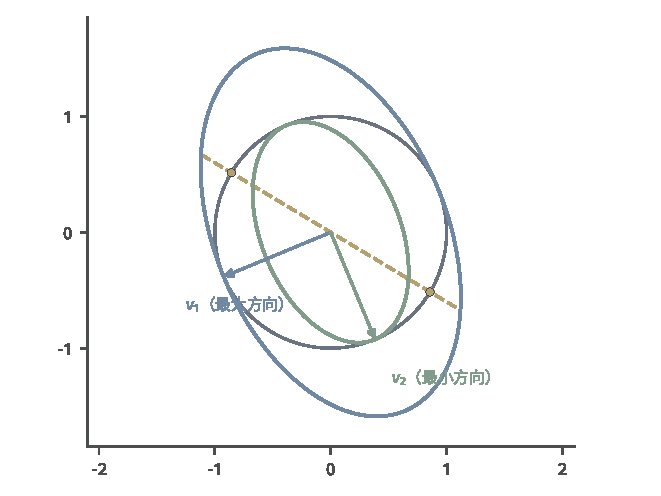
\includegraphics[width=112mm]{figures/00-shared/mathematical-preliminaries-upper/02-linear-spaces/matplotlib/ls-sphere-constrained-extremum/ls-sphere-constrained-extremum.pdf}
  \caption{单位圆约束下的极值落在特征方向。$\bm S=\left[\begin{smallmatrix}2&0.5\\0.5&1\end{smallmatrix}\right]$，
  灰圆为$\lVert\bm x\rVert=1$。蓝椭圆$\bm x^\top\bm S\bm x=\lambda_1\approx2.21$在
  $\pm\bm v_1$处与单位圆相切（最大值），绿椭圆$=\lambda_2\approx0.79$在$\pm\bm v_2$处
  相切（最小值）；黄色虚线为子空间约束直线，其上黄点是该约束下的两个极值，
  第~\ref{sec:ls-spectral-value-sensitivity}节的最小最大原理使用这种限制。
  $\lambda_{1,2}=(3\pm\sqrt2)/2$。固定复算。}
  \label{fig:ls-sphere-constrained-extremum}
\end{figure}

回到开头的对角矩阵，现在可以完成全部单位方向的比较。

\begin{example}[对角矩阵在全部单位方向上的比较]
\label{ex:ls-rayleigh-diagonal-two-by-two}
取$\bm S=\operatorname{diag}(4,1)$。每个单位向量都能写成$\bm x=(\cos\theta,\sin\theta)^\top$，其中$\theta\in[0,2\pi)$，于是
\[
 \bm x^\top\bm S\bm x=4\cos^2\theta+\sin^2\theta=1+3\cos^2\theta .
\]
由$0\leq\cos^2\theta\leq1$，它介于$1$与$4$之间：$\cos^2\theta=1$即$\bm x=\pm\bm e_1$时取最大值$4$，$\cos^2\theta=0$即$\bm x=\pm\bm e_2$时取最小值$1$。$\theta=\pi/4$时$\cos^2\theta=1/2$，得到开头的$5/2$。

可见最大值$4$与最小值$1$正是两个特征值，取到它们的方向正是特征方向，与定理~\ref{thm:matrix-analysis-rayleigh-ritz}一致；倾斜方向的值都严格介于两者之间。
\end{example}

定理不要求$\bm S$半正定。二次型可以取负值，例如$\bm S=\operatorname{diag}(1,-2)$时
\[
 \bm x^\top\bm S\bm x=x_1^2-2x_2^2 ,
\]
单位方向上的值仍介于$-2$与$1$之间，两端分别在$\pm\bm e_2$与$\pm\bm e_1$取到。

\paragraph{最优方向的唯一性}
还要区分最优值与最优方向的唯一性。最大值$\lambda_1$总是唯一的数，取到它的方向则由特征空间$\ker(\bm S-\lambda_1\bm I)$决定。

$\lambda_1$单重时，这个空间是一条直线，单位最优方向只有$\pm\bm q_1$两个，相差一个符号。$\lambda_1$重复时，空间中每个单位向量都给出最大值，例如$\bm S=\bm I$时所有单位方向都是最优的。

重根时，谱分解中的$\bm q_1$只是最优方向中的一个代表，取决于特征基的选择；最优方向组成的集合则由定理~\ref{thm:ls-spectral-projections}唯一确定。最小值的情形相同。

\paragraph{特例：$\bm S=\bm A^\top\bm A$}
一个常见的特例是$\bm S=\bm A^\top\bm A$，其中$\bm A\in\mathbb R^{m\times d}$。这时
\[
 R_{\bm A^\top\bm A}(\bm x)=\frac{\bm x^\top\bm A^\top\bm A\bm x}{\bm x^\top\bm x}=\frac{\lVert\bm A\bm x\rVert_2^2}{\lVert\bm x\rVert_2^2},
\]
即输出长度与输入长度之比的平方。

第~\ref{chap:singular-value-decomposition}章已经说明$\bm A^\top\bm A$的特征值是奇异值的平方（$d>m$时补上零）。所以定理~\ref{thm:matrix-analysis-rayleigh-ritz}给出那里最大、最小输出长度的另一种解释：单位输入的输出长度最大为$\sigma_1$，在$\bm v_1$取到；最小为$\sqrt{\lambda_d}$，其中$\lambda_d$是$\bm A^\top\bm A$的最小特征值，在它的特征方向取到。

第~\ref{sec:linear-algebra-homogeneous-estimation}节的齐次最小二乘正是在单位输入中最小化这一量。若$\bm A$有非零的零空间，最小值为零，任一单位零空间向量都最优。若$\bm A$满列秩，则$\bm A\bm x\neq\bm0$对一切$\bm x\neq\bm0$成立，$\bm A^\top\bm A\succ0$，由定理~\ref{thm:ls-symmetric-definiteness-eigenvalues}，最小值为正。

\paragraph{回到秩一逼近}
现在取$\bm S=\bm G=\bm A\bm A^\top$。由定理~\ref{thm:matrix-analysis-rayleigh-ritz}，单位方向的保留量最大为$\lambda_1(\bm G)$，恰在$\ker(\bm G-\lambda_1(\bm G)\bm I)$中的单位向量处取到。代入式~\eqref{eq:matrix-approximation-rank-one-error}，最小平方误差为
\begin{equation}
 \min_{\operatorname{rank}\bm X\leq1}\lVert\bm A-\bm X\rVert_{\mathrm F}^2=\lVert\bm A\rVert_{\mathrm F}^2-\lambda_1(\bm G) .
 \label{eq:matrix-approximation-rank-one-min-error-gram}
\end{equation}

这里只使用了第~\ref{chap:eigen-spectral-decomposition}章已经证明的谱分解。谱分解的存在不依赖本节的极值结论，本节只是用它读出极值。

\begin{example}[比较两个特征方向]
\label{ex:matrix-approximation-rank-one-eigen-directions}
沿用示例~\ref{ex:matrix-approximation-rank-one-fixed-direction}的$\bm A$。$\bm G=\bm A\bm A^\top$的元素是$\bm A$两行的内积：
\[
 g_{11}=2^2+1^2=5,\qquad g_{12}=g_{21}=2\cdot1+1\cdot2=4,\qquad g_{22}=1^2+2^2=5,
\]
即
\[
 \bm G=\begin{bmatrix}5&4\\4&5\end{bmatrix}.
\]

逐行相乘可以验证两个特征向量：
\[
 \bm G\begin{bmatrix}1\\1\end{bmatrix}=\begin{bmatrix}5+4\\4+5\end{bmatrix}=9\begin{bmatrix}1\\1\end{bmatrix},\qquad
 \bm G\begin{bmatrix}1\\-1\end{bmatrix}=\begin{bmatrix}5-4\\4-5\end{bmatrix}=\begin{bmatrix}1\\-1\end{bmatrix}.
\]
所以两个标准正交特征方向$(1,1)^\top/\sqrt2$与$(1,-1)^\top/\sqrt2$的保留量分别是$9$与$1$，重建平方误差分别是$10-9=1$与$10-1=9$。

也可以直接比较全部单位方向。取$\bm u=(\cos\theta,\sin\theta)^\top$，
\[
 \bm u^\top\bm G\bm u=5\cos^2\theta+8\cos\theta\sin\theta+5\sin^2\theta=5+4\sin2\theta ,
\]
它介于$1$与$9$之间，在$\theta=\pi/4$与$\theta=3\pi/4$分别取到最大与最小值；$\theta=0$即$\bm u=\bm e_1$时为$5$，与示例~\ref{ex:matrix-approximation-rank-one-fixed-direction}末尾的比较一致。

所以那里所取的方向$(1,1)^\top/\sqrt2$已是最优方向，而$(1,-1)^\top/\sqrt2$是最差的方向。
\end{example}

\subsection{最优解与逼近误差}
\label{sec:matrix-approximation-rank-one-solution}

\paragraph{由奇异值分解读出最优解}
上一小节用$\bm G$的特征方向给出了最优直线，现在把它与$\bm A$的奇异值分解联系起来，写出最优近似矩阵。设$\bm A\neq\bm0$，奇异值为$\sigma_1\geq\cdots\geq\sigma_r>0$。

式~\eqref{eq:ls-svd-transpose-relation}说明，$\bm G=\bm A\bm A^\top$的特征值是$\sigma_1^2,\ldots,\sigma_r^2$及$m-r$个零，左奇异向量$\bm u_i$是对应的特征向量。因此最大保留量为$\lambda_1(\bm G)=\sigma_1^2$，取$\bm u=\bm u_1$即可达到。

总平方长度也由奇异值给出：
\[
 \lVert\bm A\rVert_{\mathrm F}^2=\operatorname{tr}\bm G=\sum_{i=1}^r\sigma_i^2 .
\]
所以最小平方误差为
\begin{equation}
 \lVert\bm A\rVert_{\mathrm F}^2-\sigma_1^2=\sum_{i=2}^r\sigma_i^2 .
 \label{eq:matrix-approximation-rank-one-min-error}
\end{equation}

再求最优系数。由式~\eqref{eq:ls-svd-transpose-relation}，$\bm A^\top\bm u_1=\sigma_1\bm v_1$，所以
\[
 \bm c=\bm A^\top\bm u_1=\sigma_1\bm v_1 .
\]
把最佳方向与最优系数合成：
\begin{equation}
 \bm A_1=\bm u_1\bm u_1^\top\bm A=\bm u_1(\bm A^\top\bm u_1)^\top=\sigma_1\bm u_1\bm v_1^\top .
 \label{eq:matrix-approximation-rank-one-optimum}
\end{equation}

这是原矩阵$\bm A$的秩一近似，即和式~\eqref{eq:matrix-analysis-svd-rank-one-sum}的第一项，而不是Gram矩阵$\bm G$的秩一近似。计算的输入是$\bm A$，输出是近似矩阵$\bm A_1$；它不是某个方程的解向量。

\paragraph{计算步骤}
按上面的推导，计算秩一最优逼近只需三件事：求出保留量最大的方向，求出各列在该方向上的系数，再把两者合成。下面写出用到的变量与步骤，并用以下数据逐步演示：
\[
 \bm A=\begin{bmatrix}2&1\\1&2\end{bmatrix}.
\]
这是示例~\ref{ex:matrix-approximation-rank-one-fixed-direction}的矩阵。

变量如下。
\begin{itemize}
 \item $\sigma_1^2$与$\bm u_1\in\mathbb R^m$：$\bm G=\bm A\bm A^\top$的最大特征值与一个单位特征向量，即最大保留量与最优方向。
 \item $\bm c\in\mathbb R^d$：各列在$\bm u_1$上的投影系数，等于$\sigma_1\bm v_1$。
 \item $\bm A_1\in\mathbb R^{m\times d}$：秩一近似矩阵。
 \item $e$：平方误差$\lVert\bm A-\bm A_1\rVert_{\mathrm F}^2$，用于核对。
\end{itemize}

依次执行以下步骤。
\begin{enumerate}
 \item \textbf{求最优方向。}求$\bm G=\bm A\bm A^\top$的最大特征值$\sigma_1^2$与单位特征向量$\bm u_1$；若已有$\bm A$的奇异值分解，直接读出$\sigma_1$与$\bm u_1$。例中示例~\ref{ex:matrix-approximation-rank-one-eigen-directions}已求得
 \[
  \sigma_1^2=9,\qquad \bm u_1=\frac1{\sqrt2}\begin{bmatrix}1\\1\end{bmatrix}.
 \]

 \item \textbf{求系数。}按式~\eqref{eq:matrix-approximation-rank-one-coefficients}计算
 \[
  \bm c=\bm A^\top\bm u_1 .
 \]
 例中
 \[
  \bm c=\frac1{\sqrt2}\begin{bmatrix}2+1\\1+2\end{bmatrix}=\frac3{\sqrt2}\begin{bmatrix}1\\1\end{bmatrix}.
 \]
 它等于$\sigma_1\bm v_1$，其中$\sigma_1=3$、$\bm v_1=(1,1)^\top/\sqrt2$；已有奇异值分解时这一步可直接取$\sigma_1\bm v_1$。

 \item \textbf{合成近似矩阵。}按式~\eqref{eq:matrix-approximation-rank-one-optimum}作外积
 \[
  \bm A_1=\bm u_1\bm c^\top .
 \]
 例中
 \[
  \bm A_1=\frac1{\sqrt2}\cdot\frac3{\sqrt2}\begin{bmatrix}1&1\\1&1\end{bmatrix}=\frac32\begin{bmatrix}1&1\\1&1\end{bmatrix}.
 \]

 \item \textbf{核对误差。}求残差$\bm A-\bm A_1$的平方和，并与$\lVert\bm A\rVert_{\mathrm F}^2-\sigma_1^2$比较。例中
 \[
  \bm A-\bm A_1=\frac12\begin{bmatrix}1&-1\\-1&1\end{bmatrix},\qquad
  e=1=10-9 .
 \]
\end{enumerate}

最终得到
\[
 \bm A_1=\frac32\begin{bmatrix}1&1\\1&1\end{bmatrix}.
\]
它的四个元素都是$3/2$，两列成比例，秩为一。另一个奇异值是$\sigma_2=1$（$\bm A(1,-1)^\top=(1,-1)^\top$），平方误差$1=\sigma_2^2$，与最小误差公式一致。

同样的步骤用于示例~\ref{ex:ls-low-rank-three-columns}。这时$\bm G=\operatorname{diag}(9,4,1)$，最大特征值为$9$，$\bm u_1=\bm e_1$。系数与合成的近似矩阵为
\[
 \bm c=\bm A^\top\bm e_1=\begin{bmatrix}3\\0\\0\end{bmatrix},\qquad \bm A_1=3\bm e_1\bm e_1^\top .
\]
它只保留第一列，另两列被投影成零，平方误差为
\[
 14-9=5=4+1 .
\]

\paragraph{列重建与行重建}
这里用的是$\bm A\bm A^\top$而不是$\bm A^\top\bm A$，因为我们重建的是$\mathbb R^m$中的列向量。保留量直接等于列向量在$\bm u$上的投影长度平方之和，对应的是左奇异方向。

若改为重建行向量，同样的推导会用到$\bm A^\top\bm A$与右奇异方向$\bm v_1$。由$\bm A\bm v_1=\sigma_1\bm u_1$，得到的近似是
\[
 \bm A\bm v_1\bm v_1^\top=\sigma_1\bm u_1\bm v_1^\top ,
\]
与式~\eqref{eq:matrix-approximation-rank-one-optimum}是同一个矩阵。

这种解释依赖$\bm G$是Gram矩阵。对一般不定的对称矩阵$\bm S$，二次型值可能为负，不能把任意Rayleigh商的极值都解释成某个矩阵的最佳秩一逼近。

\paragraph{最优矩阵的唯一性}
最后区分最优近似矩阵与它的表示。$\bm A=\bm0$时$r=0$，每个方向的保留量都是零，唯一的最优近似是零矩阵。

$\sigma_1>\sigma_2$（或$r=1$）时，$\bm G$最大特征值的特征空间是一条直线，最优方向只有$\pm\bm u_1$。把$(\bm u_1,\bm v_1)$同时换成$(-\bm u_1,-\bm v_1)$不改变外积，所以最优矩阵$\bm A_1$唯一，不唯一的只是它的写法。

$\sigma_1=\sigma_2$时情况不同：最大特征值的特征空间至少二维，其中每个单位向量$\bm u$都给出最优近似$\bm u\bm u^\top\bm A$，不同的直线给出不同的矩阵。例如$\bm A=\bm I_2$时，$\bm G=\bm I_2$，每个单位向量$\bm u$的保留量都是$1$，误差都是
\[
 \lVert\bm I_2-\bm u\bm u^\top\rVert_{\mathrm F}^2=2-1=1 ;
\]
$\bm e_1\bm e_1^\top$与$\bm e_2\bm e_2^\top$就是两个不同的最优近似。

所以表示的非唯一性不等于近似矩阵的非唯一性，后者只来自最大奇异值重复。下一步保持误差标准不变，把允许保留的方向数由一个增加到$k$个。

% 第15章第3节：秩k逼近（子空间选择与迹极值、截断SVD的构造、最佳误差与最优性、最优解的唯一性）。

\section{秩\texorpdfstring{$k$}{k}逼近}
\label{sec:ls-low-rank-approximation}
\label{sec:ls-low-rank-solve}
\label{sec:ls-full-svd-solve}
\label{sec:matrix-analysis-svd-low-rank}

把共同的重建方向由一条直线扩展为$k$维子空间。与秩一情形一样，先固定子空间求系数，再选择子空间本身；用子空间的标准正交基，保留量写成一个迹，选子空间就成为迹的极值问题。由奇异值分解可以写出这个问题的解，即截断SVD；随后在Frobenius范数与谱范数下证明它的最优性，并讨论最优解何时唯一。

\subsection{子空间选择与迹极值}
\label{sec:ls-low-rank-projection-error}
\label{sec:ls-rank-k-trace}

\paragraph{固定子空间时的最优重建}
秩约束要求全部重建向量共用至多$k$个独立方向。先把这些方向张成的$k$维子空间固定下来，问每一列应当怎样重建。直观上，答案应当是把每一列正交投影到这个子空间上，这与秩一情形相同；下面把这一点写成等式。

以列标准正交的$\bm Y\in\mathbb R^{m\times k}$表示这个子空间，
\[
 \bm Y^\top\bm Y=\bm I_k ;
\]
这里不用字母$\bm V$，以免与右奇异向量矩阵混淆。列都落在$\operatorname{range}(\bm Y)$中的矩阵恰好是
\[
 \bm X=\bm Y\bm C,\qquad \bm C\in\mathbb R^{k\times d},
\]
$\bm C$的第$j$列是$\bm x_j$在这组基下的系数。由第~\ref{chap:inner-product-spaces}章的投影矩阵，$\bm Y\bm Y^\top$是到$\operatorname{range}(\bm Y)$的正交投影。

以$m=3$、$k=2$、$\bm Y=[\bm e_1,\bm e_2]$为例，按元素写出
\[
 \begin{gathered}
 \bm Y\bm Y^\top=\begin{bmatrix}1&0&0\\0&1&0\\0&0&0\end{bmatrix},\\
 \bm Y\bm C=\begin{bmatrix}c_{1,1}&\cdots&c_{1,d}\\c_{2,1}&\cdots&c_{2,d}\\0&\cdots&0\end{bmatrix}.
 \end{gathered}
\]
投影保留每一列的前两个分量、去掉第三个分量；候选矩阵的第三行只能是零，前两行可以任意选取。

\begin{lemma}[固定子空间时的正交误差分解]
\label{lem:ls-low-rank-projection-error}
设$\bm Y\in\mathbb R^{m\times k}$满足$\bm Y^\top\bm Y=\bm I_k$，则对任意$\bm C\in\mathbb R^{k\times d}$，
\begin{equation}
 \begin{aligned}
 \lVert\bm A-\bm Y\bm C\rVert_{\mathrm F}^2
 &=\lVert(\bm I-\bm Y\bm Y^\top)\bm A\rVert_{\mathrm F}^2\\
 &\qquad+\lVert\bm Y^\top\bm A-\bm C\rVert_{\mathrm F}^2,
 \end{aligned}
 \label{eq:ls-low-rank-projection-split}
\end{equation}
并且
\begin{equation}
 \lVert(\bm I-\bm Y\bm Y^\top)\bm A\rVert_{\mathrm F}^2
 =\lVert\bm A\rVert_{\mathrm F}^2-\operatorname{tr}(\bm Y^\top\bm A\bm A^\top\bm Y).
 \label{eq:ls-low-rank-projection-residual}
\end{equation}
因此固定子空间时，最优系数唯一，为$\bm C=\bm Y^\top\bm A$，最优重建是正交投影$\bm Y\bm Y^\top\bm A$。
\end{lemma}
\begin{proof}
把误差矩阵拆成两部分：
\[
 \bm A-\bm Y\bm C=(\bm I-\bm Y\bm Y^\top)\bm A+\bm Y(\bm Y^\top\bm A-\bm C).
\]
逐列看，第$j$列是$\bm r_j=(\bm I-\bm Y\bm Y^\top)\bm a_j$与$\bm Y\bm z_j$之和，其中$\bm z_j$是$\bm Y^\top\bm A-\bm C$的第$j$列。二者正交：
\[
 \bm r_j^\top\bm Y\bm z_j=\bm a_j^\top(\bm I-\bm Y\bm Y^\top)\bm Y\bm z_j
 =\bm a_j^\top(\bm Y-\bm Y\bm Y^\top\bm Y)\bm z_j=0 ,
\]
这里用到$\bm Y^\top\bm Y=\bm I_k$。又由同一关系，
\[
 \lVert\bm Y\bm z_j\rVert_2^2=\bm z_j^\top\bm Y^\top\bm Y\bm z_j=\lVert\bm z_j\rVert_2^2 .
\]
由勾股定理，误差矩阵第$j$列的平方长度是
\[
 \lVert\bm r_j\rVert_2^2+\lVert\bm z_j\rVert_2^2 ;
\]
对$j$求和即得式~\eqref{eq:ls-low-rank-projection-split}。

对第二式，同样把$\bm a_j$分解为$\bm Y\bm Y^\top\bm a_j$与$\bm r_j$两个正交部分，得
\[
 \lVert\bm r_j\rVert_2^2=\lVert\bm a_j\rVert_2^2-\lVert\bm Y^\top\bm a_j\rVert_2^2 .
\]
求和后，
\[
 \sum_j\lVert\bm Y^\top\bm a_j\rVert_2^2=\lVert\bm Y^\top\bm A\rVert_{\mathrm F}^2
 =\operatorname{tr}(\bm Y^\top\bm A\bm A^\top\bm Y).
\]
最后，式~\eqref{eq:ls-low-rank-projection-split}右端第一项与$\bm C$无关，第二项非负，且当且仅当$\bm C=\bm Y^\top\bm A$时为零。
\end{proof}

于是在固定子空间中，误差等于总平方长度减去保留量$\operatorname{tr}(\bm Y^\top\bm A\bm A^\top\bm Y)$；$k=1$、$\bm Y=\bm u$时，这正是第~\ref{sec:matrix-approximation-rank-one-coefficients}节逐列配方得到的公式。示例~\ref{ex:ls-low-rank-three-columns}中“先投影再计损失”的做法，也正是这个最优重建。

共同子空间把$d$个向量各自的最小二乘问题合成了一个矩阵近似问题：子空间共用，系数逐列由投影给出。

在上面$\bm Y=[\bm e_1,\bm e_2]$的例子中，取$\bm A=\operatorname{diag}(3,2,1)$，最优系数与最优重建为
\[
 \begin{gathered}
 \bm Y^\top\bm A=\begin{bmatrix}3&0&0\\0&2&0\end{bmatrix},\\
 \bm Y\bm Y^\top\bm A=\begin{bmatrix}3&0&0\\0&2&0\\0&0&0\end{bmatrix}.
 \end{gathered}
\]
残差只剩右下角的$1$，平方误差为
\[
 \lVert\bm A\rVert_{\mathrm F}^2-\operatorname{tr}(\bm Y^\top\bm A\bm A^\top\bm Y)=14-(9+4)=1 ,
\]
与示例~\ref{ex:ls-low-rank-three-columns}中坐标平面$\operatorname{span}\{\bm e_1,\bm e_2\}$的损失一致。

\paragraph{化为子空间的选择}
引理只处理了列都落在给定子空间中的候选。下面说明，这一化归覆盖全部秩不超过$k$的矩阵，而不只覆盖事先写成投影形式的矩阵。

设$\operatorname{rank}\bm X=s\leq k$。取$\bm X$列空间的一组标准正交基，再在$\mathbb R^m$中补充$k-s$个与之正交的单位向量（$k\leq m$，所以可以补齐），排成$\bm Y$。则$\bm X$的列都落在$\operatorname{range}(\bm Y)$中，
\[
 \bm X=\bm Y\bm C,\qquad \bm C=\bm Y^\top\bm X .
\]
由引理~\ref{lem:ls-low-rank-projection-error}，
\[
 \lVert\bm A-\bm X\rVert_{\mathrm F}^2\geq\lVert\bm A\rVert_{\mathrm F}^2-\operatorname{tr}(\bm Y^\top\bm A\bm A^\top\bm Y).
\]
反过来，每个列标准正交的$\bm Y$都给出秩不超过$k$的候选$\bm Y\bm Y^\top\bm A$，误差恰为右端。两方面合起来，
\begin{equation}
 \begin{aligned}
 &\min_{\operatorname{rank}\bm X\leq k}\lVert\bm A-\bm X\rVert_{\mathrm F}^2\\
 &\qquad=\lVert\bm A\rVert_{\mathrm F}^2-\max_{\bm Y^\top\bm Y=\bm I_k}\operatorname{tr}(\bm Y^\top\bm A\bm A^\top\bm Y),
 \end{aligned}
 \label{eq:ls-low-rank-subspace-reduction}
\end{equation}
只要右端的最大值存在；最大值的存在与取值由下面的定理~\ref{thm:matrix-analysis-trace-minimum}给出。到这里，“同时选择方向与系数”化成了“选择子空间”。

\paragraph{保留量的含义}
再看保留量本身。对$\bm Y=[\bm y_1,\ldots,\bm y_k]$按列展开：
\[
 \begin{aligned}
 \operatorname{tr}(\bm Y^\top\bm A\bm A^\top\bm Y)
 &=\sum_{l=1}^k\bm y_l^\top\bm A\bm A^\top\bm y_l\\
 &=\sum_{l=1}^k\sum_{j=1}^d(\bm y_l^\top\bm a_j)^2 .
 \end{aligned}
\]
迹把$k$个互相垂直方向上的保留量相加，$k=1$时恰好回到上一节的Rayleigh商。

保留量只依赖子空间，不依赖基的选取。记$\bm G=\bm A\bm A^\top$。把$\bm Y$换成$\bm Y\bm O$（$\bm O$为$k$阶正交矩阵）时，由迹的循环性，
\[
 \operatorname{tr}(\bm O^\top\bm Y^\top\bm G\bm Y\bm O)=\operatorname{tr}(\bm Y^\top\bm G\bm Y).
\]

据此，由式~\eqref{eq:ls-low-rank-subspace-reduction}，秩$k$逼近归结为下面的\emph{迹极值问题}：
\[
 \begin{gathered}
 \text{在}\ \bm Y^\top\bm Y=\bm I_k\ \text{下最大化}\ \operatorname{tr}(\bm Y^\top\bm G\bm Y),\\
 \bm G=\bm A\bm A^\top .
 \end{gathered}
\]

\paragraph{两个候选界}
逐列套用Rayleigh--Ritz定理只能得到每一项不超过$\lambda_1(\bm G)$，即
\[
 \operatorname{tr}(\bm Y^\top\bm G\bm Y)\leq k\lambda_1(\bm G).
\]
这个界没有用到各列互相正交的约束，一般取不到：由定理~\ref{thm:matrix-analysis-rayleigh-ritz}的取等条件，总和等于$k\lambda_1(\bm G)$要求每个$\bm y_l$都落在最大特征值的特征空间中；若$\lambda_1(\bm G)$单重，这个特征空间是一条直线，$k\geq2$时容不下$k$个互相正交的单位向量。

另一个方向是只比较由$\bm G$的特征向量组成的子空间。设$\bm G$的特征值为$\lambda_1\geq\cdots\geq\lambda_m$，对应标准正交特征向量$\bm q_1,\ldots,\bm q_m$。取$\bm Y=[\bm q_{i_1},\ldots,\bm q_{i_k}]$（下标互不相同），则$\bm y_l^\top\bm G\bm y_l=\lambda_{i_l}$，保留量为
\[
 \operatorname{tr}(\bm Y^\top\bm G\bm Y)=\lambda_{i_1}+\cdots+\lambda_{i_k}.
\]
保留前$k$个特征方向给出最大的特征值和$\sum_{i\leq k}\lambda_i$。

回到示例~\ref{ex:ls-low-rank-three-columns}，$\bm G=\operatorname{diag}(9,4,1)$。第一个界给出$2\times9=18$，超过总长度平方$14$，显然太松。三个坐标平面给出$13,10,5$，其中前两个特征方向张成的$\operatorname{span}\{\bm e_1,\bm e_2\}$最好，保留$13$、损失$1$。

一般地，由式~\eqref{eq:ls-svd-transpose-relation}，$\bm A\bm A^\top$的前$k$个特征方向可以取为左奇异向量$\bm u_1,\ldots,\bm u_k$，候选子空间就是$\operatorname{span}\{\bm u_1,\ldots,\bm u_k\}$。

\paragraph{倾斜子空间与权重}
任意倾斜的子空间会把权重分散到多个特征方向上，它是否仍不能超过特征值和，需要看清正交约束对权重的限制。仍取$\bm G=\operatorname{diag}(9,4,1)$，考虑倾斜平面
\[
 \bm Y=\begin{bmatrix}1&0\\0&1/\sqrt2\\0&1/\sqrt2\end{bmatrix}.
\]
它在三个特征方向$\bm e_1,\bm e_2,\bm e_3$上的权重$w_i=\lVert\bm Y^\top\bm e_i\rVert_2^2$依次是$\bm Y$各行的平方长度：
\[
 w_1=1,\qquad w_2=\frac12,\qquad w_3=\frac12 .
\]
保留量就是特征值的加权和：
\[
 \operatorname{tr}(\bm Y^\top\bm G\bm Y)=9\cdot1+4\cdot\frac12+1\cdot\frac12=\frac{23}2<13 .
\]
权重各不超过$1$，总和为$k=2$。这个平面把第二个特征方向上的一半权重让给了较小的第三个特征值，因而保留得更少。

下面的定理说明这对任意实对称矩阵、任意$k$维子空间都成立；同时也回答迹能否低于后$k$个特征值之和。

\begin{theorem}[迹极值]
\label{thm:matrix-analysis-trace-minimum}
设$\bm S\in\mathbb R^{m\times m}$实对称，特征值$\lambda_1\geq\cdots\geq\lambda_m$，对应标准正交特征向量$\bm q_1,\ldots,\bm q_m$，$1\leq k\leq m$。对满足$\bm Y^\top\bm Y=\bm I_k$的$\bm Y\in\mathbb R^{m\times k}$，
\begin{equation}
 \sum_{i=m-k+1}^{m}\lambda_i\leq\operatorname{tr}(\bm Y^\top\bm S\bm Y)\leq\sum_{i=1}^{k}\lambda_i,
 \label{eq:matrix-analysis-trace-minimum}
\end{equation}
上界由$\bm Y=[\bm q_1,\ldots,\bm q_k]$取到，下界由$\bm Y=[\bm q_{m-k+1},\ldots,\bm q_m]$取到。若$k<m$且$\lambda_k>\lambda_{k+1}$，则上界取等当且仅当$\operatorname{range}(\bm Y)=\operatorname{span}\{\bm q_1,\ldots,\bm q_k\}$。
\end{theorem}
\begin{proof}
由谱定理，$\bm S=\sum_i\lambda_i\bm q_i\bm q_i^\top$，故
\[
 \operatorname{tr}(\bm Y^\top\bm S\bm Y)
 =\sum_{i=1}^m\lambda_i\operatorname{tr}(\bm Y^\top\bm q_i\bm q_i^\top\bm Y)
 =\sum_{i=1}^m\lambda_iw_i,
\]
其中$w_i=\lVert\bm Y^\top\bm q_i\rVert_2^2$。权重受两条限制。

第一，$\bm P=\bm Y\bm Y^\top$是到$\operatorname{range}(\bm Y)$的正交投影，满足$\bm P=\bm P^\top\bm P$，所以
\[
 w_i=\bm q_i^\top\bm P\bm q_i=\bm q_i^\top\bm P^\top\bm P\bm q_i=\lVert\bm P\bm q_i\rVert_2^2 .
\]
正交投影不增加长度，所以$0\leq w_i\leq\lVert\bm q_i\rVert_2^2=1$。

第二，记$\bm Q=[\bm q_1,\ldots,\bm q_m]$，它是正交矩阵，右乘正交矩阵不改变Frobenius范数，于是
\[
 \sum_{i=1}^mw_i=\lVert\bm Y^\top\bm Q\rVert_{\mathrm F}^2=\lVert\bm Y^\top\rVert_{\mathrm F}^2=\operatorname{tr}(\bm Y^\top\bm Y)=k .
\]
也就是说，总量为$k$的权重分配给各个特征值，每个特征值至多分到$1$。

直观上，要使加权和最大，应把权重全部放在最大的$k$个特征值上。用$\lambda_k$作为分界，可以把这一直观写成恒等式：
\[
 \begin{aligned}
 \sum_{i=1}^m\lambda_iw_i-\sum_{i=1}^k\lambda_i
 &=\sum_{i\leq k}(\lambda_i-\lambda_k)(w_i-1)+\sum_{i>k}(\lambda_i-\lambda_k)w_i\\
 &\qquad+\lambda_k\Bigl(\sum_{i=1}^mw_i-k\Bigr).
 \end{aligned}
\]
展开右端即可核对。最后一项因$\sum_iw_i=k$而为零。$i\leq k$时$\lambda_i-\lambda_k\geq0$、$w_i-1\leq0$；$i>k$时$\lambda_i-\lambda_k\leq0$、$w_i\geq0$。所以右端每一项都不大于零，上界成立。

上界可以取到：$\bm Y=[\bm q_1,\ldots,\bm q_k]$时$w_i$在$i\leq k$时为$1$、其余为$0$，迹等于$\sum_{i\leq k}\lambda_i$。

取等条件也可以从这个恒等式读出。若$\lambda_k>\lambda_{k+1}$，则$i>k$时$\lambda_i-\lambda_k<0$，上界取等迫使$w_i=0$，即$\bm Y^\top\bm q_i=\bm0$。于是$\operatorname{range}(\bm Y)$与$\bm q_{k+1},\ldots,\bm q_m$都正交，含于$\operatorname{span}\{\bm q_1,\ldots,\bm q_k\}$；两者都是$k$维的，所以相等。

反之，若$\operatorname{range}(\bm Y)=\operatorname{span}\{\bm q_1,\ldots,\bm q_k\}$，则$i\leq k$时$\bm P\bm q_i=\bm q_i$、$i>k$时$\bm P\bm q_i=\bm0$，迹等于上界。

下界由上界得到。$-\bm S$的特征值按降序为$-\lambda_m\geq\cdots\geq-\lambda_1$，对应特征向量依次为$\bm q_m,\ldots,\bm q_1$。对$-\bm S$应用上界，得
\[
 -\operatorname{tr}(\bm Y^\top\bm S\bm Y)\leq-\sum_{i=m-k+1}^m\lambda_i ,
\]
等号在$\bm Y=[\bm q_{m-k+1},\ldots,\bm q_m]$时成立。
\end{proof}

在倾斜平面的例子中，恒等式右端的三类项分别是
\[
 (9-4)(1-1)=0,\qquad (4-4)\Bigl(\frac12-1\Bigr)=0,\qquad (1-4)\cdot\frac12=-\frac32 .
\]
合计$-\tfrac32$，正是$\tfrac{23}2-13$：亏损全部来自让给第三个特征值的那一半权重。

\paragraph{回到低秩逼近}
取$\bm S=\bm G=\bm A\bm A^\top$。它的特征值是$\sigma_1^2\geq\cdots\geq\sigma_r^2$，再补上$m-r$个零；$k<r$时前$k$个之和为$\sum_{i\leq k}\sigma_i^2$。于是任意$k$维子空间最多保留
\begin{equation}
 \max_{\bm Y^\top\bm Y=\bm I_k}\operatorname{tr}(\bm Y^\top\bm A\bm A^\top\bm Y)=\sum_{i=1}^k\sigma_i^2 ,
 \label{eq:ls-low-rank-max-retained}
\end{equation}
式~\eqref{eq:ls-low-rank-subspace-reduction}右端的最大值存在，并由$\operatorname{span}\{\bm u_1,\ldots,\bm u_k\}$取到。在示例~\ref{ex:ls-low-rank-three-columns}中，这确认任意倾斜平面的保留量都不超过$13$，坐标平面$\operatorname{span}\{\bm e_1,\bm e_2\}$已是最优的平面。

对一般的对称矩阵$\bm S$，迹极值界照样成立，但只有在当前这种半正定的Gram情形，迹才表示投影保留的长度平方。下一小节把最优子空间上的投影重建写成具体的矩阵。

\subsection{截断SVD的构造}
\label{sec:ls-truncated-svd-construction}

\subsubsection{主要思想}

上一小节确定了最优子空间，还没有写出最优重建本身。设$\bm A$的奇异值分解写成和式~\eqref{eq:matrix-analysis-svd-rank-one-sum}，
\[
 \bm A=\sum_{i=1}^r\sigma_i\bm u_i\bm v_i^\top ,
\]
其中$r=\operatorname{rank}\bm A$，$\sigma_1\geq\cdots\geq\sigma_r>0$。$1\leq k<r$时最优子空间可取为$\operatorname{span}\{\bm u_1,\ldots,\bm u_k\}$，即
\[
 \bm Y=\bm U_k=[\bm u_1,\ldots,\bm u_k].
\]
由引理~\ref{lem:ls-low-rank-projection-error}，最优重建是$\bm U_k\bm U_k^\top\bm A$。要把它化简，只需看$\bm U_k^\top$作用在每个$\bm u_i$上的结果。

以$r=3$、$k=2$为例，由$\bm u_i$标准正交，按元素写出
\[
 \bm U_2^\top\bm u_1=\begin{bmatrix}1\\0\end{bmatrix},\qquad
 \bm U_2^\top\bm u_2=\begin{bmatrix}0\\1\end{bmatrix},\qquad
 \bm U_2^\top\bm u_3=\begin{bmatrix}0\\0\end{bmatrix}.
\]
于是$\bm U_2\bm U_2^\top\bm u_i$在$i=1,2$时还原为$\bm u_i$，在$i=3$时为零。一般地，$\bm U_k^\top\bm u_i$在$i\leq k$时等于$\bm e_i$、在$i>k$时等于$\bm0$，所以
\[
 \begin{aligned}
 \bm U_k\bm U_k^\top\bm A
 &=\sum_{i=1}^r\sigma_i\bm U_k(\bm U_k^\top\bm u_i)\bm v_i^\top\\
 &=\sum_{i=1}^k\sigma_i\bm u_i\bm v_i^\top .
 \end{aligned}
\]
也就是说，把$\bm A$的各列正交投影到前$k$个左奇异方向上，等于只保留SVD和式的前$k$项。

把这个由子空间优化推导出的矩阵记下来。对整数$k\geq0$，称
\begin{equation}
\begin{gathered}
\bm A_k=\sum_{i=1}^{\min(k,r)}\sigma_i\bm u_i\bm v_i^\top
 =\bm U_k\bm\Sigma_k\bm V_k^\top\\
k\geq0
\end{gathered}
\label{eq:matrix-analysis-truncated-svd}
\end{equation}
为$\bm A$的\term{截断SVD}（truncated SVD），其中$k\leq r$时$\bm\Sigma_k=\operatorname{diag}(\sigma_1,\ldots,\sigma_k)$，$\bm V_k=[\bm v_1,\ldots,\bm v_k]$。两种边界情形与第~\ref{sec:matrix-approximation-problem}节的直接回答一致：$k=0$时和式为空，$\bm A_0=\bm0$；$k\geq r$时保留了全部项，$\bm A_k=\bm A$。

$\bm A_k$满足秩约束。$k\leq r$时，
\[
 \bm A_k\bm v_i=\sigma_i\bm u_i\quad(i\leq k),\qquad
 \bm A_k\bm v_i=\bm0\quad(i>k),
\]
所以列空间恰为$\operatorname{span}\{\bm u_1,\ldots,\bm u_k\}$，$\operatorname{rank}\bm A_k=k$。

\subsubsection{算法实现}

截断SVD的输入是$\bm A$已经求出的SVD与秩预算$k$，输出是$\bm A_k$或它的三个因子。计算本身不迭代：取出前$k$组奇异值与奇异向量，相乘即可。下面用以下示例中的矩阵逐步演示；它的一个奇异方向是倾斜的，并且有重奇异值。

\begin{example}[有重奇异值的三阶截断]
\label{ex:matrix-approximation-truncated-three-by-three}
取
\[
 \bm A=\begin{bmatrix}3&2&0\\2&3&0\\0&0&1\end{bmatrix}.
\]
令
\[
 \bm u_1=\frac1{\sqrt2}\begin{bmatrix}1\\1\\0\end{bmatrix},\qquad
 \bm u_2=\frac1{\sqrt2}\begin{bmatrix}1\\-1\\0\end{bmatrix},\qquad
 \bm u_3=\begin{bmatrix}0\\0\\1\end{bmatrix},
\]
它们标准正交，且
\[
 \bm A\bm u_1=5\bm u_1,\qquad\bm A\bm u_2=\bm u_2,\qquad\bm A\bm u_3=\bm u_3 .
\]
$\bm A$对称、特征值非负，所以可取$\bm v_i=\bm u_i$，奇异值为$5,1,1$。下面分别取$k=1$与$k=2$。
\end{example}

\paragraph{变量}
\begin{itemize}
 \item $k$：秩预算；$r$：$\bm A$的秩，即正奇异值的个数。
 \item $\sigma_i,\bm u_i,\bm v_i$：已经求出的奇异值与配对的左右奇异向量。
 \item $\bm U_k\in\mathbb R^{m\times k}$、$\bm\Sigma_k$、$\bm V_k\in\mathbb R^{d\times k}$：截取出的三个因子。
 \item $\bm W=\bm\Sigma_k\bm V_k^\top\in\mathbb R^{k\times d}$：缩放后的右因子，即最优系数矩阵。
 \item $\bm A_k$：截断SVD；$\bm E_k=\bm A-\bm A_k$：重建残差，只在核验时形成。
\end{itemize}

\paragraph{输入与预处理}
先核对$k$是满足$0\leq k\leq\min(m,d)$的整数，并由正奇异值的个数确定$r$。$k=0$时直接输出零矩阵；$k\geq r$时直接输出$\bm A$。其余情形下，确认奇异值按非增顺序排列；若SVD例程给出的顺序不同，就把奇异值连同配对的左右奇异向量一起重新排序。配对不能打乱，因为每一项$\sigma_i\bm u_i\bm v_i^\top$都要求$\bm A\bm v_i=\sigma_i\bm u_i$。

例中$r=3$，$k=1,2$都满足$1\leq k<r$，奇异值$5,1,1$已按非增顺序排列。

\paragraph{计算步骤}
\begin{enumerate}
 \item \textbf{截取因子。}取前$k$组奇异值与奇异向量，
 \[
  \bm U_k=[\bm u_1,\ldots,\bm u_k],\qquad
  \bm\Sigma_k=\operatorname{diag}(\sigma_1,\ldots,\sigma_k),
 \]
 $\bm V_k=[\bm v_1,\ldots,\bm v_k]$。若只需要压缩存储，到这一步即可输出三个因子，不必形成$m\times d$的矩阵。

 例中$k=1$时$\bm U_1=\bm V_1=\bm u_1$，$\bm\Sigma_1=5$；$k=2$时
 \[
  \bm U_2=\bm V_2=\frac1{\sqrt2}\begin{bmatrix}1&1\\1&-1\\0&0\end{bmatrix},\qquad
  \bm\Sigma_2=\begin{bmatrix}5&0\\0&1\end{bmatrix}.
 \]

 \item \textbf{缩放右因子。}把$\bm V_k^\top$的第$i$行乘以$\sigma_i$：
 \begin{equation}
  \bm W=\bm\Sigma_k\bm V_k^\top .
  \label{eq:ls-truncated-svd-coefficients}
 \end{equation}
 由$\bm A^\top\bm u_i=\sigma_i\bm v_i$，$\bm W=\bm U_k^\top\bm A$，它正是引理~\ref{lem:ls-low-rank-projection-error}中的最优系数。

 例中$k=2$时
 \[
  \bm W=\frac1{\sqrt2}\begin{bmatrix}5&5&0\\1&-1&0\end{bmatrix},
 \]
 第一行即$k=1$时的$\bm W$。

 \item \textbf{相乘重建。}按式~\eqref{eq:matrix-analysis-truncated-svd}计算
 \[
  \bm A_k=\bm U_k\bm W=\sum_{i=1}^k\sigma_i\bm u_i\bm v_i^\top .
 \]
 例中$k=1$时只有一项：
 \[
  \bm A_1=5\bm u_1\bm u_1^\top=\frac52\begin{bmatrix}1&1&0\\1&1&0\\0&0&0\end{bmatrix},
 \]
 左上四项均为$5/2$，其余为零。$k=2$时再加上第二项
 \[
  \bm u_2\bm u_2^\top=\frac12\begin{bmatrix}1&-1&0\\-1&1&0\\0&0&0\end{bmatrix},
 \]
 左上角的对角元变为$5/2+1/2=3$，非对角元变为$5/2-1/2=2$：
 \[
  \bm A_2=\begin{bmatrix}3&2&0\\2&3&0\\0&0&0\end{bmatrix}.
 \]

 \item \textbf{核验残差。}需要核验时，形成$\bm E_k=\bm A-\bm A_k$，计算它的Frobenius范数与谱范数，并检查$\operatorname{rank}\bm A_k=k$。

 例中$k=1$时
 \[
  \bm E_1=\begin{bmatrix}1/2&-1/2&0\\-1/2&1/2&0\\0&0&1\end{bmatrix}.
 \]
 Frobenius范数平方为
 \[
  \lVert\bm E_1\rVert_{\mathrm F}^2=4\times\frac14+1=2 ,
 \]
 即$\lVert\bm E_1\rVert_{\mathrm F}=\sqrt2$。

 谱范数要看$\bm E_1$的作用。它可以写成
 \[
  \bm E_1=\bm u_2\bm u_2^\top+\bm u_3\bm u_3^\top ,
 \]
 是到$\operatorname{span}\{\bm u_2,\bm u_3\}$的正交投影，它把该平面内的单位向量原样送出，把$\bm u_1$送到零，所以$\lVert\bm E_1\rVert_2=1$。

 $k=2$时
 \[
  \bm E_2=\bm e_3\bm e_3^\top ,
 \]
 只有右下角一个元素$1$，两种范数都是$1$。
\end{enumerate}

最终得到例中的两个截断SVD：
\[
 \begin{gathered}
 \bm A_1=\frac52\begin{bmatrix}1&1&0\\1&1&0\\0&0&0\end{bmatrix},\\
 \bm A_2=\begin{bmatrix}3&2&0\\2&3&0\\0&0&0\end{bmatrix}.
 \end{gathered}
\]
$\bm A_1$两列相同、秩为一，$\bm A_2$左上块行列式$9-4=5\neq0$、秩为二；两者都只保留了$\bm A$在前$k$个奇异方向上的部分。

这个例子还显示了重奇异值带来的变化。由于$\sigma_2=\sigma_3$，把$\bm u_2$与$\bm u_3$的次序交换也是$\bm A$的一个SVD。按它截断，第三步加上的第二项是$\bm u_3\bm u_3^\top$，得到
\[
 \bm A_2'=\bm A_1+\bm u_3\bm u_3^\top=\begin{bmatrix}5/2&5/2&0\\5/2&5/2&0\\0&0&1\end{bmatrix},
\]
残差$\bm u_2\bm u_2^\top$的两种范数同样为$1$。$\bm A_2\neq\bm A_2'$而误差相同：截断位置处奇异值重复时，“前$k$个奇异方向”有不同的选法，算法的输出依赖SVD例程给出的那一组。

图~\ref{fig:ls-low-rank-truncation}画出截断的几何：单位圆经$\bm A$变成椭圆，秩一近似把椭圆压成主轴方向的线段，残留的谱范数误差恰为舍弃的$\sigma_2$。

\begin{figure*}[htbp]
  \centering
  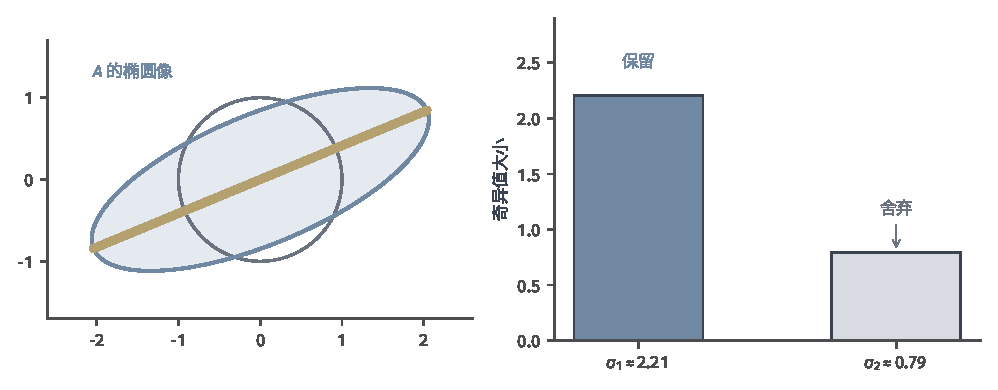
\includegraphics[width=168.998mm]{figures/00-shared/mathematical-preliminaries-upper/02-linear-spaces/matplotlib/ls-low-rank-truncation/ls-low-rank-truncation.pdf}
  \caption{低秩截断的几何。$\bm A=\left[\begin{smallmatrix}2&0.5\\0.5&1\end{smallmatrix}\right]$，
  灰圆为单位圆，蓝椭圆为$\bm A$的像。左：黄粗线段为秩一近似$\bm A_1=\sigma_1\bm v_1\bm v_1^\top$
  的像，椭圆被压成长$2\sigma_1$的线段；右：$\sigma_1\approx2.21$（保留）、$\sigma_2\approx0.79$
  （舍弃），算子范数误差$\lVert\bm A-\bm A_1\rVert_2=\sigma_2$。$\sigma_{1,2}=(3\pm\sqrt2)/2$。
  固定复算。}
  \label{fig:ls-low-rank-truncation}
\end{figure*}

\subsubsection{算法分析}

\paragraph{表示与计算代价}
截断SVD的好处在于表示代价。直接存储$\bm A$需要$md$个数；保存因子$\bm U_k$、$\sigma_1,\ldots,\sigma_k$与$\bm V_k$只需
\[
 k(m+d+1)
\]
个数。用$\bm A_k$乘向量时按
\[
 \bm A_k\bm x=\bm U_k\bigl(\bm\Sigma_k(\bm V_k^\top\bm x)\bigr)
\]
的顺序计算，依次需要约$dk$、$k$、$mk$次乘法，共$O(k(m+d))$次运算，而直接用$\bm A$乘向量需要$O(md)$次。

例如$m=d=1000$、$k=10$时，存储由$10^6$个数降为$20010$个数。形成完整的$\bm A_k=\bm U_k\bm W$约需$mdk$次乘法，只在需要矩阵本身或核验残差时才做。

这些是表示与后续作用的代价，不包括计算SVD本身的代价；后者取决于所用的数值算法，本书不作分析。

\paragraph{用途的区别}
第~\ref{chap:solution-error-regularization}章的截断SVD求解也用到$\bm A_k$，但那里是用它的伪逆稳定地求解方程；这里$\bm A_k$本身就是要评价的近似对象，评价标准是重建误差。$\bm A_k$的误差有多大、它在全部秩不超过$k$的矩阵中是否最好，由下一小节回答。

\subsection{最佳误差与最优性}
\label{sec:ls-truncated-svd-optimality}

\paragraph{截断SVD的误差}
截断SVD舍弃了后$r-k$项，误差应当由舍弃的奇异值决定。先把它算出来。设$0\leq k<r$，余下的部分是
\[
 \bm A-\bm A_k=\sum_{i=k+1}^r\sigma_i\bm u_i\bm v_i^\top .
\]
它仍由两组标准正交向量和降序的正系数$\sigma_{k+1}\geq\cdots\geq\sigma_r$组成，可以照第~\ref{sec:ls-svd-matrix-size}节的方法读出它的大小。

先看谱范数。把输入写成$\bm x=\sum_{i=1}^dc_i\bm v_i$，则
\[
 (\bm A-\bm A_k)\bm x=\sum_{i=k+1}^r\sigma_ic_i\bm u_i .
\]
由$\bm u_i$标准正交，
\[
 \lVert(\bm A-\bm A_k)\bm x\rVert_2^2=\sum_{i=k+1}^r\sigma_i^2c_i^2\leq\sigma_{k+1}^2\lVert\bm x\rVert_2^2,
\]
等号在$\bm x=\bm v_{k+1}$时成立。

再看Frobenius范数。由$\bm u_i^\top\bm u_j=\delta_{i,j}$，
\[
 (\bm A-\bm A_k)^\top(\bm A-\bm A_k)=\sum_{i=k+1}^r\sigma_i^2\bm v_i\bm v_i^\top ,
\]
取迹得Frobenius范数平方$\sum_{i>k}\sigma_i^2$。于是
\begin{equation}
\begin{gathered}
\lVert\bm A-\bm A_k\rVert_2=\sigma_{k+1}\\
\lVert\bm A-\bm A_k\rVert_{\mathrm F}
 =\Bigl(\sum_{i=k+1}^r\sigma_i^2\Bigr)^{1/2}.
\end{gathered}
\label{eq:ls-truncated-errors}
\end{equation}
Frobenius平方误差也可以由引理~\ref{lem:ls-low-rank-projection-error}读出：
\[
 \lVert\bm A\rVert_{\mathrm F}^2-\operatorname{tr}(\bm U_k^\top\bm A\bm A^\top\bm U_k)=\sum_{i\leq r}\sigma_i^2-\sum_{i\leq k}\sigma_i^2 .
\]
示例~\ref{ex:matrix-approximation-truncated-three-by-three}中$k=1$时，式~\eqref{eq:ls-truncated-errors}给出$\sqrt{1^2+1^2}=\sqrt2$与$\sigma_2=1$，与直接计算的$\bm E_1$一致。

\begin{example}[对角矩阵的截断误差]
\label{ex:ls-truncated-svd-diagonal}
取示例~\ref{ex:ls-low-rank-three-columns}中的$\bm A=\operatorname{diag}(3,2,1)$，奇异值为$3,2,1$，可取$\bm u_i=\bm v_i=\bm e_i$。截断得
\[
 \bm A_1=\operatorname{diag}(3,0,0),\qquad\bm A_2=\operatorname{diag}(3,2,0),
\]
残差为
\[
 \bm A-\bm A_1=\operatorname{diag}(0,2,1),\qquad\bm A-\bm A_2=\operatorname{diag}(0,0,1).
\]
$k=1$时平方误差$2^2+1^2=5$，谱范数误差$2$；$k=2$时平方误差与谱范数误差都是$1$。两者都与式~\eqref{eq:ls-truncated-errors}一致：
\[
 5=\sigma_2^2+\sigma_3^2,\qquad 2=\sigma_2,\qquad 1=\sigma_3 .
\]

平方误差$5$是只保留坐标直线$\bm e_1$时的损失，平方误差$1$是最佳坐标平面$\operatorname{span}\{\bm e_1,\bm e_2\}$的损失。
\end{example}

\paragraph{为什么还要比较全部候选}
两种误差记录的内容不同：Frobenius平方误差汇总所有舍弃方向，谱范数误差只记录最坏的单位输入方向。式~\eqref{eq:ls-truncated-errors}只是这一构造的误差，尚需证明其他秩不超过$k$的矩阵不能更小。

Frobenius范数的结论由上一小节的化归和迹极值得到。谱范数不能这样处理，因为
\[
 \lVert\bm M\rVert_2\leq\lVert\bm M\rVert_{\mathrm F},
\]
Frobenius误差的下界推不出谱范数误差的下界，需要另作证明。

谱范数下界的想法是：秩不超过$k$的$\bm X$至少把一个$(d-k)$维子空间送到零，这个子空间一定与前$k+1$个右奇异方向相交；在交点处，$\bm A-\bm X$的作用就是$\bm A$本身的作用，而$\bm A$在前$k+1$个方向上至少放大$\sigma_{k+1}$倍。

下面用一个例子说明这一想法。取$\bm A=\operatorname{diag}(3,2,1)$、$k=1$，并取一个不同于截断SVD的秩一候选：
\[
 \bm X=\begin{bmatrix}3&2&0\\0&0&0\\0&0&0\end{bmatrix}.
\]
它的核是$\{\bm x:3x_1+2x_2=0\}$，与$\operatorname{span}\{\bm e_1,\bm e_2\}$交于
\[
 \bm x=\frac1{\sqrt{13}}\begin{bmatrix}2\\-3\\0\end{bmatrix}.
\]
在这个单位向量上$\bm X\bm x=\bm0$，于是
\[
 (\bm A-\bm X)\bm x=\bm A\bm x=\frac1{\sqrt{13}}\begin{bmatrix}6\\-6\\0\end{bmatrix},
\]
它的长度为
\[
 \lVert\bm A\bm x\rVert_2=\sqrt{72/13}\approx2.353\geq\sigma_2=2 .
\]
所以这个候选的谱范数误差至少为$2.353$，不比截断SVD好。下面的定理对任意候选作同样的论证。

\begin{theorem}[Eckart--Young--Mirsky最佳低秩逼近]
\label{thm:ls-best-low-rank}
\label{thm:matrix-analysis-best-low-rank}
设$\bm A\in\mathbb R^{m\times d}$的秩为$r$，奇异值为$\sigma_1\geq\cdots\geq\sigma_r>0$。对$0\leq k<r$，
\begin{align}
 \min_{\operatorname{rank}\bm X\leq k}\lVert\bm A-\bm X\rVert_2
 &=\sigma_{k+1},
 \label{eq:matrix-analysis-best-rank-k-spectral}\\
 \min_{\operatorname{rank}\bm X\leq k}\lVert\bm A-\bm X\rVert_{\mathrm F}
 &=\Bigl(\sum_{i=k+1}^r\sigma_i^2\Bigr)^{1/2},
 \label{eq:matrix-analysis-best-rank-k-frobenius}
\end{align}
两个最小值都由截断SVD$\bm A_k$达到。
\end{theorem}
\begin{proof}
由式~\eqref{eq:ls-truncated-errors}，$\bm A_k$的两种误差恰为右端，只需证明任意秩不超过$k$的$\bm X$误差都不更小。$k=0$时只有$\bm X=\bm0$，结论即式~\eqref{eq:ls-truncated-errors}，下设$k\geq1$。

Frobenius情形。按第~\ref{sec:ls-low-rank-projection-error}节的做法，把$\bm X$的列空间补成一个$k$维子空间，取其标准正交基组成$\bm Y$，则$\bm X=\bm Y\bm C$。由引理~\ref{lem:ls-low-rank-projection-error}、定理~\ref{thm:matrix-analysis-trace-minimum}与式~\eqref{eq:matrix-analysis-frobenius-norm}，
\[
 \begin{aligned}
 \lVert\bm A-\bm X\rVert_{\mathrm F}^2
 &\geq\lVert\bm A\rVert_{\mathrm F}^2-\operatorname{tr}(\bm Y^\top\bm A\bm A^\top\bm Y)\\
 &\geq\sum_{i=1}^r\sigma_i^2-\sum_{i=1}^k\sigma_i^2=\sum_{i=k+1}^r\sigma_i^2 .
 \end{aligned}
\]

谱范数情形。由秩零度定理~\ref{thm:ls-rank-nullity}，
\[
 \dim\ker\bm X=d-\operatorname{rank}\bm X\geq d-k .
\]
子空间$\operatorname{span}\{\bm v_1,\ldots,\bm v_{k+1}\}$的维数为$k+1$（$k+1\leq r\leq d$）。两者维数之和超过$d$，由维数公式，它们有非零公共向量；取其中的单位向量$\bm x=\sum_{i=1}^{k+1}c_i\bm v_i$，$\sum_ic_i^2=1$。由$\bm X\bm x=\bm0$，
\begin{equation}
 \lVert(\bm A-\bm X)\bm x\rVert_2
 =\lVert\bm A\bm x\rVert_2
 =\Bigl(\sum_{i=1}^{k+1}\sigma_i^2c_i^2\Bigr)^{1/2}
 \geq\sigma_{k+1},
 \label{eq:ls-spectral-lower-bound}
\end{equation}
所以$\lVert\bm A-\bm X\rVert_2\geq\sigma_{k+1}$。
\end{proof}

在上面的秩一候选中，$c_1=2/\sqrt{13}$、$c_2=-3/\sqrt{13}$，式~\eqref{eq:ls-spectral-lower-bound}的中间量为
\[
 \sigma_1^2c_1^2+\sigma_2^2c_2^2=9\cdot\frac4{13}+4\cdot\frac9{13}=\frac{72}{13}\geq\sigma_2^2=4 ,
\]
与直接计算一致。

这一结论最早由Eckart与Young给出\scite{eckart1936}。定理覆盖任意秩不超过$k$的矩阵，而不只覆盖事先选定的投影形式：Frobenius情形借助第~\ref{sec:ls-low-rank-projection-error}节的化归把任意候选归入某个子空间，谱范数情形则直接利用候选矩阵的核。两种范数下的最小误差都由舍弃的奇异值决定：谱范数看最大的舍弃值$\sigma_{k+1}$，Frobenius范数看全部舍弃值的平方和。

\subsection{最优解的唯一性}
\label{sec:matrix-approximation-low-rank-uniqueness}

\paragraph{Frobenius情形}
最小误差唯一，达到最小误差的矩阵却未必唯一。示例~\ref{ex:matrix-approximation-truncated-three-by-three}中的$\bm A_2$与$\bm A_2'$已经说明了这一点。问题是：什么条件下最优矩阵只有一个？在有效的秩预算$1\leq k<r$下，Frobenius情形的答案由迹极值的取等条件决定，关键是截断位置两侧的奇异值是否有间隙。

\begin{theorem}[Frobenius最佳逼近的唯一性]
\label{thm:ls-best-low-rank-uniqueness}
设$1\leq k<r$且$\sigma_k>\sigma_{k+1}$，则$\bm A_k$是$\min_{\operatorname{rank}\bm X\leq k}\lVert\bm A-\bm X\rVert_{\mathrm F}$的唯一最优解。
\end{theorem}
\begin{proof}
设$\bm X$达到最小值，按定理~\ref{thm:ls-best-low-rank}的证明取$\bm Y$，写$\bm X=\bm Y\bm C$。证明中的两个不等号都须取等。第一个取等，由式~\eqref{eq:ls-low-rank-projection-split}得$\bm C=\bm Y^\top\bm A$，即
\[
 \bm X=\bm Y\bm Y^\top\bm A .
\]

第二个取等，即
\[
 \operatorname{tr}(\bm Y^\top\bm A\bm A^\top\bm Y)=\sum_{i=1}^k\sigma_i^2 .
\]
$\bm A\bm A^\top$的第$k$与第$k+1$个特征值为$\sigma_k^2>\sigma_{k+1}^2$，由定理~\ref{thm:matrix-analysis-trace-minimum}的取等条件，$\operatorname{range}(\bm Y)=\operatorname{span}\{\bm u_1,\ldots,\bm u_k\}$。

到同一子空间的正交投影是同一个矩阵，故$\bm Y\bm Y^\top=\bm U_k\bm U_k^\top$，从而
\[
 \bm X=\bm U_k\bm U_k^\top\bm A=\bm A_k .
\]
\end{proof}

$k=1$时，条件$\sigma_1>\sigma_2$正是第~\ref{sec:matrix-approximation-rank-one-solution}节秩一最优解唯一的条件。

间隙条件也确定了$\bm A_k$本身：$\sigma_k>\sigma_{k+1}$时，$\operatorname{span}\{\bm u_1,\ldots,\bm u_k\}$是$\bm A\bm A^\top$前$k$个特征值对应的特征空间之和，不随SVD的选取改变，$\bm A_k=\bm U_k\bm U_k^\top\bm A$也就与所选的奇异向量无关。示例~\ref{ex:matrix-approximation-truncated-three-by-three}中$k=1$时$\sigma_1=5>\sigma_2=1$，$\bm A_1$唯一；$k=2$时$\sigma_2=\sigma_3$，定理不适用。

截断跨过相等的正奇异值时，唯一性失败。例如$\bm A=\operatorname{diag}(2,1,1)$、$k=2$，下面两个矩阵都是最优解：
\[
 \operatorname{diag}(2,1,0),\qquad\operatorname{diag}(2,0,1).
\]
它们的残差分别是$\operatorname{diag}(0,0,1)$与$\operatorname{diag}(0,1,0)$，平方误差都是$1=\sigma_3^2$。这时“前$k$个奇异向量”本身就有不同选法，每种选法给出一个最优矩阵；三阶例中的$\bm A_2$与$\bm A_2'$也是这种情形。

\paragraph{谱范数情形}
谱范数下的最优矩阵即使有间隙也不唯一，所以间隙条件不能直接当成谱范数的唯一性保证。先说明对角矩阵的谱范数。$\bm D=\operatorname{diag}(a_1,\ldots,a_m)$满足
\[
 \lVert\bm D\bm x\rVert_2^2=\sum_ia_i^2x_i^2\leq\max_ia_i^2\,\lVert\bm x\rVert_2^2 ,
\]
在绝对值最大的对角元所在的坐标向量处取等，故
\[
 \lVert\bm D\rVert_2=\max_i\lvert a_i\rvert .
\]
取$\bm A=\operatorname{diag}(3,2,1)$、$k=1$，候选$\bm X=\operatorname{diag}(t,0,0)$给出残差$\operatorname{diag}(3-t,2,1)$，于是
\[
 \lVert\bm A-\bm X\rVert_2=\max(\lvert3-t\rvert,2).
\]
$1\leq t\leq5$时它都等于最小值$2$，尽管$\sigma_1=3>\sigma_2=2$。例如$t=2$时残差是$\operatorname{diag}(1,2,1)$，最坏方向仍是$\bm e_2$。谱范数只看最坏方向，最坏方向之外的偏差在一定范围内可以随意改变。

Frobenius范数则不同：同一族候选的平方误差是
\[
 \lVert\bm A-\bm X\rVert_{\mathrm F}^2=(3-t)^2+5 ,
\]
只在$t=3$时取到最小值$5$。

\paragraph{边界情形与适用范围}
边界情形$k=0$与$k\geq r$已在第~\ref{sec:matrix-approximation-problem}节回答，最优矩阵分别是$\bm0$与$\bm A$本身，不需要套用间隙判据。

本节的最优性依赖两个前提：允许集合是全部秩不超过$k$的矩阵，误差是谱范数或Frobenius范数。额外要求近似矩阵非负或因子稀疏时，允许集合缩小，$\bm A_k$可能不再可行。改用逐元素加权的平方误差
\[
 \sum_{i,j}w_{i,j}(a_{i,j}-x_{i,j})^2
\]
时，误差一般不再按正交投影分解，引理~\ref{lem:ls-low-rank-projection-error}失效。这些情形下截断SVD一般不再是最优解，最优性需要重新论证；下一节处理其中能够化归的一类加权误差。

% 第15章第4节：加权逼近与广义Rayleigh商（广义Rayleigh商的极值、加权低秩逼近）。

\section{加权逼近与广义Rayleigh商}
\label{sec:ls-generalized-rayleigh}

前两节都用欧氏长度：单位方向按$\bm u^\top\bm u=1$规定，重建误差按各元素平方和计算。各坐标的单位或重要性不同时，长度往往按第~\ref{chap:inner-product-spaces}章的加权内积度量。度量一变，有两处跟着改变：规定“单位方向”的长度变了，比较重建误差的标准也变了。

本节先处理前一处：保持二次型不变，改用加权长度规定单位方向，得到广义Rayleigh商及其极值。再处理后一处：在行、列权重可以分离的误差下研究低秩逼近，并看到它的最佳方向正是由广义Rayleigh商选出的。广义Rayleigh商还为后面的图谱松弛提供工具：卷九的谱划分把平衡约束写成按顶点度加权的长度，再用广义Rayleigh商的极值给出离散划分问题的松弛下界，可参考\BookChapterRef{chap:spectral-partition}{卷九“谱划分”章}。

\subsection{广义Rayleigh商的极值}
\label{sec:ls-generalized-eigen-reduction}
\label{sec:ls-generalized-eigen-check}

保持$\bm S=\operatorname{diag}(4,1)$不变，改用$\bm B=\operatorname{diag}(9,1)$规定长度，即要求
\[
 \bm x^\top\bm B\bm x=9x_1^2+x_2^2=1 .
\]
沿第一坐标方向，满足约束的向量是$\pm\bm e_1/3$；沿第二坐标方向，满足约束的向量仍是$\pm\bm e_2$。两者的二次型值分别为
\[
 \Bigl(\frac{\bm e_1}3\Bigr)^{\!\top}\bm S\,\frac{\bm e_1}3=4\cdot\Bigl(\frac13\Bigr)^2=\frac49,\qquad
 \bm e_2^\top\bm S\bm e_2=1 .
\]
在欧氏约束下最优的$\bm e_1$方向，现在不如$\bm e_2$方向。

可见改变长度标准会改变答案。而且与示例~\ref{ex:ls-rayleigh-diagonal-two-by-two}之前的讨论一样，比较两个坐标方向还不够，必须比较全部满足加权约束的方向。与欧氏情形相同，先把约束化为一个不随缩放改变的商。
\begin{definition}[广义Rayleigh商]
\label{def:ls-generalized-rayleigh-quotient}
设$\bm S\in\mathbb R^{d\times d}$对称，$\bm B\in\mathbb R^{d\times d}$对称正定。对$\bm x\neq\bm0$，称
\begin{equation}
 R_{\bm S,\bm B}(\bm x)=\frac{\bm x^\top\bm S\bm x}{\bm x^\top\bm B\bm x}
 \label{eq:ls-generalized-rayleigh-quotient}
\end{equation}
为$\bm S$关于$\bm B$的\term{广义Rayleigh商}（generalized Rayleigh quotient）。
\end{definition}
$\bm B$正定保证分母$\bm x^\top\bm B\bm x$对一切$\bm x\neq\bm0$为正，商有定义。把$\bm x$换成$c\bm x$（$c\neq0$）时分子分母同乘$c^2$，商不变。

对任意$\bm x\neq\bm0$，令$\bm u=\bm x/\sqrt{\bm x^\top\bm B\bm x}$，则
\[
 \bm u^\top\bm B\bm u=1,\qquad R_{\bm S,\bm B}(\bm x)=\bm u^\top\bm S\bm u ;
\]
反过来，约束$\bm x^\top\bm B\bm x=1$上的二次型值就是广义Rayleigh商。所以求广义Rayleigh商的极值，等价于在$\bm x^\top\bm B\bm x=1$上比较$\bm x^\top\bm S\bm x$。

$\bm B=\bm I$时，广义Rayleigh商恰好回到普通Rayleigh商。两者比较的是同一个二次型$\bm x^\top\bm S\bm x$，差别只在于用哪种长度规定“单位输入”：普通Rayleigh商用欧氏长度，广义Rayleigh商用加权长度$\lVert\bm x\rVert_{\bm B}$。

\subsubsection{主要思想}

\paragraph{把加权长度换成欧氏长度}
加权约束$\bm x^\top\bm B\bm x=1$的困难在于它不是欧氏单位球面，第~\ref{sec:ls-rayleigh-extremal}节的结论不能直接使用。思路是换一个坐标，使加权长度在新坐标中成为欧氏长度。

先看开头的例子。约束可以改写成两个平方之和：
\[
 9x_1^2+x_2^2=(3x_1)^2+x_2^2 .
\]
令$z_1=3x_1$、$z_2=x_2$，约束就成为欧氏单位圆$z_1^2+z_2^2=1$。二次型也用新坐标表示，由$x_1=z_1/3$得
\[
 4x_1^2+x_2^2=\frac49z_1^2+z_2^2 .
\]
于是加权约束下的问题，变成了对角矩阵$\operatorname{diag}(4/9,1)$在欧氏单位圆上的普通Rayleigh商问题。

一般的$\bm B$不是对角矩阵，但同样可以写成平方和。设$\bm L$是上三角矩阵，令$\bm z=\bm L\bm x$。二阶时按元素写出
\[
 \begin{bmatrix}z_1\\z_2\end{bmatrix}
 =\begin{bmatrix}l_{1,1}&l_{1,2}\\0&l_{2,2}\end{bmatrix}
 \begin{bmatrix}x_1\\x_2\end{bmatrix}
 =\begin{bmatrix}l_{1,1}x_1+l_{1,2}x_2\\l_{2,2}x_2\end{bmatrix},
\]
展开平方和得
\[
 \begin{aligned}
 z_1^2+z_2^2
 &=l_{1,1}^2x_1^2+2l_{1,1}l_{1,2}x_1x_2+(l_{1,2}^2+l_{2,2}^2)x_2^2\\
 &=\bm x^\top
 \begin{bmatrix}l_{1,1}^2&l_{1,1}l_{1,2}\\l_{1,1}l_{1,2}&l_{1,2}^2+l_{2,2}^2\end{bmatrix}
 \bm x .
 \end{aligned}
\]
中间的矩阵正是$\bm L^\top\bm L$。所以只要$\bm B=\bm L^\top\bm L$，加权长度$\bm x^\top\bm B\bm x$在新坐标中就是欧氏长度$\bm z^\top\bm z$。开头的例子对应$\bm L=\operatorname{diag}(3,1)$。

这样的$\bm L$总是存在。由定理~\ref{thm:ls-gram-factor}，正定的$\bm B$可以写成$\bm B=\bm L^\top\bm L$，其中$\bm L$可逆。于是$\bm x=\bm L^{-1}\bm z$，且$\bm x\neq\bm0$当且仅当$\bm z\neq\bm0$。

\paragraph{化为普通Rayleigh商}
把$\bm x=\bm L^{-1}\bm z$代入分子与分母，得
\[
 \bm x^\top\bm B\bm x=(\bm L\bm x)^\top(\bm L\bm x)=\bm z^\top\bm z,\qquad
 \bm x^\top\bm S\bm x=\bm z^\top\bm L^{-\top}\bm S\bm L^{-1}\bm z ,
\]
其中$\bm L^{-\top}$表示$(\bm L^{-1})^\top$。记
\begin{equation}
 \bm C=\bm L^{-\top}\bm S\bm L^{-1}.
 \label{eq:ls-generalized-rayleigh-reduced-matrix}
\end{equation}
由$\bm S$对称，
\[
 \bm C^\top=\bm L^{-\top}\bm S^\top\bm L^{-1}=\bm C ,
\]
所以$\bm C$仍是实对称矩阵。广义Rayleigh商在新坐标中写成
\begin{equation}
 R_{\bm S,\bm B}(\bm x)=\frac{\bm z^\top\bm C\bm z}{\bm z^\top\bm z}=R_{\bm C}(\bm L\bm x).
 \label{eq:ls-generalized-rayleigh-reduction}
\end{equation}
加权约束问题就化成了$\bm C$的普通Rayleigh商问题，可以直接应用定理~\ref{thm:matrix-analysis-rayleigh-ritz}。

这一化归只用到Gram因子与换元，不需要矩阵平方根、多元微分或Lagrange乘子法。开头的例子中$\bm C=\operatorname{diag}(4/9,1)$，正是上面按元素得到的矩阵。

\paragraph{换回原坐标}
$\bm C$的最优方向在新坐标中，还要换回原坐标。若$\bm C\bm z=\mu\bm z$，令$\bm v=\bm L^{-1}\bm z$，则
\[
 \bm L^{-\top}\bm S\bm v=\mu\bm L\bm v .
\]
两边左乘$\bm L^\top$，得
\[
 \bm S\bm v=\mu\bm L^\top\bm L\bm v=\mu\bm B\bm v .
\]
反过来，若$\bm S\bm v=\mu\bm B\bm v$且$\bm v\neq\bm0$，左乘$\bm L^{-\top}$并令$\bm z=\bm L\bm v$，就得到$\bm C\bm z=\mu\bm z$。所以，$\bm C$的特征对与下面方程的解一一对应。

\begin{definition}[广义特征值]
\label{def:matrix-analysis-generalized-eigenvalue}
对实对称$\bm S$与对称正定$\bm B$，称满足
\begin{equation}
\begin{gathered}
\bm S\bm v=\mu\bm B\bm v\\
\bm v\neq\bm0
\end{gathered}
\label{eq:matrix-analysis-generalized-eigenproblem}
\end{equation}
的$\mu$为广义特征值，$\bm v$为属于$\mu$的广义特征向量，求解它们的问题称为\term{广义特征问题}（generalized eigenvalue problem）。
\end{definition}

广义特征值不依赖Gram因子$\bm L$的选取。由$\bm S-\mu\bm B=\bm L^\top(\bm C-\mu\bm I)\bm L$，
\[
 \det(\bm S-\mu\bm B)=(\det\bm L)^2\det(\bm C-\mu\bm I),
\]
而$\det\bm L\neq0$，所以广义特征值恰是$\det(\bm S-\mu\bm B)=0$的根，也就是$\bm C$的特征值。不同的$\bm L$给出不同的$\bm C$，特征值却相同。

$\bm C$对称，由谱定理，这些根全是实数，按重数计共有$d$个，下面记为$\mu_1\geq\cdots\geq\mu_d$。

\paragraph{极值与最优方向}
把定理~\ref{thm:matrix-analysis-rayleigh-ritz}用于$\bm C$并换回原坐标，就得到加权约束问题的解。

\begin{theorem}[广义Rayleigh商的极值]
\label{thm:ls-generalized-rayleigh-extremal}
设$\bm S$对称、$\bm B$对称正定，广义特征值为$\mu_1\geq\cdots\geq\mu_d$。则对一切$\bm x\neq\bm0$，
\begin{equation}
 \mu_d\leq R_{\bm S,\bm B}(\bm x)\leq\mu_1 .
 \label{eq:ls-generalized-rayleigh-extremal}
\end{equation}
$R_{\bm S,\bm B}(\bm x)=\mu_1$当且仅当$\bm S\bm x=\mu_1\bm B\bm x$，$R_{\bm S,\bm B}(\bm x)=\mu_d$当且仅当$\bm S\bm x=\mu_d\bm B\bm x$。因此，在约束$\bm x^\top\bm B\bm x=1$上，$\bm x^\top\bm S\bm x$的最大值为$\mu_1$，最优解是满足$\bm v^\top\bm B\bm v=1$的属于$\mu_1$的广义特征向量；最小值的情形相同。
\end{theorem}
\begin{proof}
取$\bm B=\bm L^\top\bm L$与$\bm C=\bm L^{-\top}\bm S\bm L^{-1}$如上。$\bm C$的特征值就是$\mu_1\geq\cdots\geq\mu_d$。对$\bm x\neq\bm0$，令$\bm z=\bm L\bm x\neq\bm0$，由$R_{\bm S,\bm B}(\bm x)=R_{\bm C}(\bm z)$及定理~\ref{thm:matrix-analysis-rayleigh-ritz}，得$\mu_d\leq R_{\bm S,\bm B}(\bm x)\leq\mu_1$。

同一定理还说明，$R_{\bm C}(\bm z)=\mu_1$当且仅当$\bm C\bm z=\mu_1\bm z$。由上面的一一对应，这又当且仅当$\bm S\bm x=\mu_1\bm B\bm x$。$\bm C$确有属于$\mu_1$的特征向量，所以上界能够取到。最小值同理。

最后，约束$\bm x^\top\bm B\bm x=1$上的二次型值就是广义Rayleigh商，所以它的最大值为$\mu_1$，且只在满足$\bm S\bm x=\mu_1\bm B\bm x$与$\bm x^\top\bm B\bm x=1$的$\bm x$处取到。
\end{proof}

\paragraph{\texorpdfstring{$\bm B$}{B}正交的广义特征向量}
上面只用到$\bm C$两端的特征向量。对$\bm C$应用完整的谱分解，还能得到全部广义特征向量的结构：它们可以选得关于加权内积$\langle\cdot,\cdot\rangle_{\bm B}$互相正交。

\begin{theorem}[$\bm B$正交的广义特征向量]
\label{thm:ls-generalized-eigen-b-orthogonal}
设$\bm S$对称、$\bm B$对称正定，广义特征值为$\mu_1\geq\cdots\geq\mu_d$。则存在$\bm v_1,\ldots,\bm v_d$，使
\begin{equation}
 \bm S\bm v_i=\mu_i\bm B\bm v_i,\qquad \bm v_i^\top\bm B\bm v_j=\delta_{i,j}\quad(i,j=1,\ldots,d).
 \label{eq:ls-generalized-eigen-b-orthogonal}
\end{equation}
记$\bm V=[\bm v_1,\ldots,\bm v_d]$，$\bm M=\operatorname{diag}(\mu_1,\ldots,\mu_d)$，上式等价于$\bm V^\top\bm B\bm V=\bm I$与$\bm V^\top\bm S\bm V=\bm M$。
\end{theorem}
\begin{proof}
由谱定理，$\bm C=\bm Z\bm M\bm Z^\top$，其中$\bm Z=[\bm z_1,\ldots,\bm z_d]$为正交矩阵，$\bm C\bm z_i=\mu_i\bm z_i$。令$\bm V=\bm L^{-1}\bm Z$，即$\bm v_i=\bm L^{-1}\bm z_i$。由上面的一一对应，$\bm S\bm v_i=\mu_i\bm B\bm v_i$。又
\[
\begin{gathered}
 \bm V^\top\bm B\bm V=\bm Z^\top\bm L^{-\top}\bm L^\top\bm L\bm L^{-1}\bm Z=\bm Z^\top\bm Z=\bm I,\\
 \bm V^\top\bm S\bm V=\bm Z^\top\bm L^{-\top}\bm S\bm L^{-1}\bm Z=\bm Z^\top\bm C\bm Z=\bm M .
\end{gathered}
\]
逐元素比较第一式即得$\bm v_i^\top\bm B\bm v_j=\delta_{i,j}$。
\end{proof}

$\bm V$可逆，所以任意$\bm x$都能写成$\bm x=\sum_ia_i\bm v_i$。由定理，
\[
 \bm x^\top\bm B\bm x=\sum_{i=1}^da_i^2,\qquad \bm x^\top\bm S\bm x=\sum_{i=1}^d\mu_ia_i^2 .
\]
广义Rayleigh商再次成为特征值的加权平均。这与普通情形完全平行，只是坐标改成了$\bm B$正交的广义特征向量。

至此两端极值都已求出。若还需要刻画中间的广义特征值，可以对$\bm C$使用第~\ref{sec:ls-spectral-value-sensitivity}节的Courant--Fischer最小最大原理（定理~\ref{thm:matrix-analysis-courant-fischer}），再按$\bm z=\bm L\bm x$换回原坐标。

\paragraph{用开头的例子核对}
最后回到开头的二维例子，把上面的结论逐一落实，并与直接比较全部可行方向的结果对照。

\begin{example}[加权约束下的最优方向]
\label{ex:ls-generalized-rayleigh-diagonal}
取$\bm S=\operatorname{diag}(4,1)$与$\bm B=\operatorname{diag}(9,1)$，在加权约束$\bm x^\top\bm B\bm x=1$下求$\bm x^\top\bm S\bm x$的最大值、最小值与最优方向。

由$\bm L=\operatorname{diag}(3,1)$得$\bm C=\operatorname{diag}(4/9,1)$。由定理~\ref{thm:matrix-analysis-rayleigh-ritz}，$R_{\bm C}$的最大值为$1$，在$\bm z=\pm\bm e_2$取到；最小值为$4/9$，在$\bm z=\pm\bm e_1$取到。换回原坐标$\bm v=\bm L^{-1}\bm z$，得到
\[
 \text{最大方向}\ \pm\bm e_2,\qquad \text{最小方向}\ \pm\frac{\bm e_1}{3}.
\]

两者都满足加权单位约束：
\[
 \bm e_2^\top\bm B\bm e_2=1,\qquad \Bigl(\frac{\bm e_1}{3}\Bigr)^{\!\top}\bm B\,\frac{\bm e_1}{3}=\frac99=1 .
\]
它们也满足广义特征方程：
\[
 \bm S\bm e_2=\bm e_2=1\cdot\bm B\bm e_2,\qquad
 \bm S\frac{\bm e_1}{3}=\frac43\bm e_1=\frac49\cdot\bm B\frac{\bm e_1}{3},
\]
分别属于$1$与$4/9$；又$\bm e_2^\top\bm B(\bm e_1/3)=0$，满足$\bm B$正交。

不经化归，也可以直接比较全部可行方向。约束给出$x_2^2=1-9x_1^2$，其中$x_1^2\in[0,1/9]$，于是
\[
 \bm x^\top\bm S\bm x=4x_1^2+1-9x_1^2=1-5x_1^2\in\Bigl[\frac49,1\Bigr].
\]
最大值$1$在$x_1=0$即$\pm\bm e_2$处取到，最小值$4/9$在$x_1^2=1/9$即$\pm\bm e_1/3$处取到，与化归的结果一致。

对照示例~\ref{ex:ls-rayleigh-diagonal-two-by-two}：同一个$\bm S$在欧氏约束下的最大方向是$\bm e_1$。加权约束让沿$\bm e_1$的可行向量缩短为$\bm e_1/3$，最大方向就换成了$\bm e_2$。
\end{example}

\subsubsection{算法实现}

上面的例子中$\bm L$是对角矩阵，可以直接求逆。一般情形下，计算也按化归的顺序进行：先求Gram因子，再形成$\bm C$，对$\bm C$作谱分解，最后换回原坐标；换元通过因子分解与三角求解完成，不必显式形成$\bm L^{-1}$。输入是对称的$\bm S$与对称正定的$\bm B$，输出是所需的广义特征值与满足$\bm v^\top\bm B\bm v=1$的广义特征向量。下面用以下新的二维示例逐步演示。

\begin{example}[按三角求解的步骤计算]
\label{ex:matrix-approximation-generalized-cholesky}
取
\[
 \bm S=\begin{bmatrix}2&0\\0&3\end{bmatrix},\qquad
 \bm B=\begin{bmatrix}4&0\\0&1\end{bmatrix},
\]
在约束$\bm x^\top\bm B\bm x=1$下求$\bm x^\top\bm S\bm x$的最大值、最小值与最优方向。
\end{example}

\paragraph{变量}
\begin{itemize}
 \item $\bm L\in\mathbb R^{d\times d}$：$\bm B$的上三角Gram因子，满足$\bm B=\bm L^\top\bm L$。
 \item $\bm W\in\mathbb R^{d\times d}$：中间矩阵$\bm W=\bm L^{-\top}\bm S$。
 \item $\bm C\in\mathbb R^{d\times d}$：化归后的对称矩阵$\bm C=\bm W\bm L^{-1}$。
 \item $\mu_i$与$\bm z_i$：$\bm C$的特征值与单位特征向量，$\mu_i$按降序排列。
 \item $\bm v_i$：换回原坐标后的广义特征向量。
\end{itemize}

\paragraph{输入与预处理}
用第~\ref{sec:ls-cholesky}节的Cholesky分解求出$\bm B=\bm G\bm G^\top$，其中$\bm G$是对角元为正的下三角矩阵，再取
\[
 \bm L=\bm G^\top ,
\]
它是上三角矩阵，满足$\bm B=\bm L^\top\bm L$。若分解中某个开方量不为正，说明$\bm B$不是正定矩阵，正定化归不能继续使用，停止并报告。

例中$\bm B$是对角矩阵，Cholesky分解直接对对角元开方：
\[
 \bm L=\begin{bmatrix}2&0\\0&1\end{bmatrix}.
\]

\paragraph{计算步骤}
\begin{enumerate}
 \item \textbf{形成$\bm W$。}解三角方程组
 \begin{equation}
  \bm L^\top\bm W=\bm S .
  \label{eq:ls-generalized-solve-w}
 \end{equation}
 $\bm L^\top$是下三角矩阵，对$\bm S$的每一列按式~\eqref{eq:ls-forward-substitution}作前代。

 例中$\bm L^\top=\operatorname{diag}(2,1)$，每个方程只含一个未知元：$2w_{1,1}=2$，$w_{2,2}=3$，非对角元的方程右端为零。于是
 \[
  \bm W=\begin{bmatrix}1&0\\0&3\end{bmatrix}.
 \]

 \item \textbf{形成$\bm C$。}由$\bm C=\bm W\bm L^{-1}$得$\bm C\bm L=\bm W$，转置后成为
 \begin{equation}
  \bm L^\top\bm C^\top=\bm W^\top ,
  \label{eq:ls-generalized-solve-c}
 \end{equation}
 仍是以下三角矩阵为系数的方程组，再作一次前代。$\bm C$对称，解出的$\bm C^\top$就是$\bm C$；舍入误差会使算出的两半略有差别，通常取$(\bm C+\bm C^\top)/2$再进入下一步，以保持对称结构。

 例中$2c_{1,1}=1$，$c_{2,2}=3$，于是
 \[
  \bm C=\begin{bmatrix}1/2&0\\0&3\end{bmatrix}.
 \]

 \item \textbf{对$\bm C$作谱分解。}对对称矩阵$\bm C$作正交谱分解，按降序取出特征值与单位特征向量；只需要最大值或最小值时，只取相应的一对。例中
 \[
  \mu_1=3,\quad \bm z_1=\bm e_2;\qquad \mu_2=\frac12,\quad \bm z_2=\bm e_1 .
 \]

 \item \textbf{换回原坐标。}对每个所需的$\bm z_i$解三角方程组
 \begin{equation}
  \bm L\bm v_i=\bm z_i ,
  \label{eq:ls-generalized-recover-v}
 \end{equation}
 $\bm L$是上三角矩阵，按式~\eqref{eq:ls-back-substitution}作回代。由$\bm v_i^\top\bm B\bm v_i=\bm z_i^\top\bm z_i=1$，所得$\bm v_i$自动满足加权单位约束。

 例中$\bm L\bm v_1=\bm e_2$与$\bm L\bm v_2=\bm e_1$分别给出
 \[
  \bm v_1=\begin{bmatrix}0\\1\end{bmatrix},\qquad \bm v_2=\begin{bmatrix}1/2\\0\end{bmatrix}.
 \]

 \item \textbf{核验。}在原坐标中计算广义特征残差$\bm S\bm v_i-\mu_i\bm B\bm v_i$与加权长度$\bm v_i^\top\bm B\bm v_i$，确认前者接近零、后者接近$1$。例中
 \[
  \bm S\bm v_1=\begin{bmatrix}0\\3\end{bmatrix}=3\,\bm B\bm v_1,\qquad
  \bm S\bm v_2=\begin{bmatrix}1\\0\end{bmatrix}=\frac12\begin{bmatrix}2\\0\end{bmatrix}=\frac12\,\bm B\bm v_2 ,
 \]
 两个残差都为零。加权长度为
 \[
  \bm v_1^\top\bm B\bm v_1=1,\qquad \bm v_2^\top\bm B\bm v_2=\Bigl(\frac12\Bigr)^2\cdot4=1 .
 \]
\end{enumerate}

最终得到加权约束下的最大值、最小值与最优方向。例中
\[
 \begin{aligned}
 \max_{\bm x^\top\bm B\bm x=1}\bm x^\top\bm S\bm x&=3, &&\text{在}\ \pm\begin{bmatrix}0\\1\end{bmatrix}\ \text{取到};\\
 \min_{\bm x^\top\bm B\bm x=1}\bm x^\top\bm S\bm x&=\frac12, &&\text{在}\ \pm\begin{bmatrix}1/2\\0\end{bmatrix}\ \text{取到}.
 \end{aligned}
\]

与欧氏约束比较：$\bm S$的普通Rayleigh商最大为$3$、最小为$2$，最优直线同样是两条坐标轴。这里加权没有改变最优直线，却把最小值由$2$变成$1/2$，因为沿$\bm e_1$满足加权约束的向量缩短为$\bm e_1/2$。与示例~\ref{ex:ls-generalized-rayleigh-diagonal}合起来看，长度标准既可能改变最优方向，也可能只改变最优值。

\subsubsection{算法分析}

\paragraph{运算量}
形成$\bm C$只用到Cholesky分解与以三角矩阵为系数的求解，代价都是$O(d^3)$次运算；之后的主要代价在对称特征值计算，所用算法本书不作分析。只需要最大或最小的广义特征对时，也必须先完成同样的换元，因为$\bm S$本身的特征向量一般不是广义特征向量。

\paragraph{为什么不改求普通特征问题}
另一种看似直接的做法是把$\bm S\bm v=\mu\bm B\bm v$左乘$\bm B^{-1}$，改求普通特征问题
\[
 \bm B^{-1}\bm S\bm v=\mu\bm v .
\]
由$\bm B^{-1}=\bm L^{-1}\bm L^{-\top}$，
\[
 \bm B^{-1}\bm S=\bm L^{-1}\bm L^{-\top}\bm S=\bm L^{-1}\bm C\bm L ,
\]
它与$\bm C$相似，特征值相同；但$\bm B^{-1}\bm S$一般不对称，谱定理不能用于它。

看一个具体的例子。取
\[
 \bm S=\begin{bmatrix}2&1\\1&2\end{bmatrix},\qquad
 \bm B=\begin{bmatrix}2&0\\0&1\end{bmatrix},
\]
则
\[
 \bm B^{-1}\bm S=\begin{bmatrix}1&1/2\\1&2\end{bmatrix},
\]
它不对称。它的特征多项式与特征值为
\[
 \mu^2-3\mu+\frac32=0,\qquad \mu_{1,2}=\frac{3\pm\sqrt3}{2}.
\]
由第一行$(1-\mu)x_1+\tfrac12x_2=0$得$x_2=2(\mu-1)x_1$，取$x_1=1$，特征向量为
\[
 \bm v_1=\begin{bmatrix}1\\1+\sqrt3\end{bmatrix},\qquad
 \bm v_2=\begin{bmatrix}1\\1-\sqrt3\end{bmatrix}.
\]
这两个向量就是广义特征向量。它们关于$\bm B$正交，在欧氏内积下却不正交：
\[
 \bm v_1^\top\bm B\bm v_2=2+(1-3)=0,\qquad
 \bm v_1^\top\bm v_2=1+(1-3)=-1\neq0 .
\]
所以不能对$\bm B^{-1}\bm S$套用谱定理与欧氏正交特征基的结论。前面两个二维例子里$\bm B^{-1}\bm S$恰好是对角矩阵，只是特殊情形。

\paragraph{正定性的作用}
本小节的化归依赖$\bm B$正定。若$\bm B$不是正定矩阵，$\bm x^\top\bm B\bm x$不再定义长度：$\bm B$半正定而奇异时，存在$\bm x\neq\bm0$使分母为零；$\bm B$不定时，$\bm x^\top\bm B\bm x$可以为负。这时也不存在可逆的$\bm L$使$\bm B=\bm L^\top\bm L$：若有这样的$\bm L$，则$\bm x\neq\bm0$时$\bm L\bm x\neq\bm0$，
\[
 \bm x^\top\bm B\bm x=\lVert\bm L\bm x\rVert_2^2>0 ,
\]
$\bm B$就是正定的。

于是化归无从进行，约束问题甚至可能没有极值。例如$\bm S=\bm I$、$\bm B=\operatorname{diag}(1,0)$时，约束$x_1^2=1$不限制$x_2$，而
\[
 \bm x^\top\bm S\bm x=1+x_2^2
\]
没有上界。这类更一般的广义特征问题不在此展开。

\subsection{加权低秩逼近}
\label{sec:matrix-approximation-weighted-low-rank}

\subsubsection{主要思想}

\paragraph{加权误差}
现在改变重建误差的度量。设$\bm A\in\mathbb R^{m\times d}$的各行表示不同的量，重要性或单位不同；各列表示不同的样本，可信程度也不同。给定对称正定的行权重$\bm\Omega_{\mathrm r}\in\mathbb R^{m\times m}$与列权重$\bm\Omega_{\mathrm c}\in\mathbb R^{d\times d}$，用
\begin{equation}
 E(\bm X)=\operatorname{tr}\bigl((\bm A-\bm X)^\top\bm\Omega_{\mathrm r}(\bm A-\bm X)\bm\Omega_{\mathrm c}\bigr)
 \label{eq:matrix-approximation-weighted-error}
\end{equation}
度量$\bm X$的误差，并在$\operatorname{rank}\bm X\leq k$下求其最小值，称为\term{加权低秩逼近}（weighted low-rank approximation）。$\bm\Omega_{\mathrm r}=\bm I$、$\bm\Omega_{\mathrm c}=\bm I$时它就是上一节的Frobenius平方误差。

先看两个权重都是对角矩阵的情形，记
\[
 \bm\Omega_{\mathrm r}=\operatorname{diag}(\omega_1,\ldots,\omega_m),\qquad
 \bm\Omega_{\mathrm c}=\operatorname{diag}(\tau_1,\ldots,\tau_d),
\]
并记$\bm M=\bm A-\bm X$。矩阵$\bm M^\top\bm\Omega_{\mathrm r}\bm M$的第$(j,j)$元是
\[
 (\bm M^\top\bm\Omega_{\mathrm r}\bm M)_{j,j}=\sum_{i=1}^m\omega_im_{i,j}^2 ;
\]
右乘$\bm\Omega_{\mathrm c}$后它乘上$\tau_j$，再对$j$求迹，得
\[
 E(\bm X)=\sum_{i=1}^m\sum_{j=1}^d\omega_i\tau_j(a_{i,j}-x_{i,j})^2 .
\]
$m=d=2$时按元素写出是
\[
 \begin{aligned}
 E(\bm X)={}&\omega_1\tau_1(a_{1,1}-x_{1,1})^2+\omega_1\tau_2(a_{1,2}-x_{1,2})^2\\
 &+\omega_2\tau_1(a_{2,1}-x_{2,1})^2+\omega_2\tau_2(a_{2,2}-x_{2,2})^2 .
 \end{aligned}
\]
即第$(i,j)$个元素的平方偏差乘以权重$\omega_i\tau_j$。所以这一类误差包含逐元素加权，但要求权重能分离成行因子与列因子的乘积。

\paragraph{化为普通的Frobenius误差}
与上一小节一样，用Gram因子把加权换成普通长度。对角情形先按元素看：取$\bm K=\operatorname{diag}(\sqrt{\omega_1},\ldots,\sqrt{\omega_m})$与$\bm N=\operatorname{diag}(\sqrt{\tau_1},\ldots,\sqrt{\tau_d})$，则
\[
 (\bm K\bm M\bm N)_{i,j}=\sqrt{\omega_i}\,m_{i,j}\sqrt{\tau_j},\qquad
 (\bm K\bm M\bm N)_{i,j}^2=\omega_i\tau_jm_{i,j}^2 ,
\]
对全部元素求和，正好是上面的$E(\bm X)$。

一般情形同样成立。由定理~\ref{thm:ls-gram-factor}，存在可逆的$\bm K$与$\bm N$，使
\[
 \bm\Omega_{\mathrm r}=\bm K^\top\bm K,\qquad \bm\Omega_{\mathrm c}=\bm N\bm N^\top
\]
（对$\bm\Omega_{\mathrm c}$取$\bm N^\top$为它的Gram因子）。由迹的循环性，
\[
 \begin{aligned}
 \lVert\bm K\bm M\bm N\rVert_{\mathrm F}^2
 &=\operatorname{tr}(\bm N^\top\bm M^\top\bm K^\top\bm K\bm M\bm N)\\
 &=\operatorname{tr}(\bm M^\top\bm\Omega_{\mathrm r}\bm M\bm N\bm N^\top)
 =E(\bm X).
 \end{aligned}
\]
于是
\begin{equation}
 E(\bm X)=\lVert\bm K(\bm A-\bm X)\bm N\rVert_{\mathrm F}^2 ,
 \label{eq:matrix-approximation-weighted-frobenius}
\end{equation}
加权误差是变换后矩阵的普通Frobenius误差。

\paragraph{秩约束不变}
令
\begin{equation}
 \widetilde{\bm A}=\bm K\bm A\bm N,\qquad \bm Z=\bm K\bm X\bm N,
 \label{eq:matrix-approximation-weighted-transform}
\end{equation}
则$E(\bm X)=\lVert\widetilde{\bm A}-\bm Z\rVert_{\mathrm F}^2$。

还要确认秩约束在这个变换下不变。乘积的列空间含于左因子的列空间，所以$\operatorname{rank}\bm Z\leq\operatorname{rank}\bm X$；又$\bm X=\bm K^{-1}\bm Z\bm N^{-1}$，同理$\operatorname{rank}\bm X\leq\operatorname{rank}\bm Z$，故二者相等。

于是$\bm X\mapsto\bm K\bm X\bm N$把秩不超过$k$的矩阵一一地变为秩不超过$k$的矩阵，原问题等价于对$\widetilde{\bm A}$作普通的低秩逼近。由定理~\ref{thm:ls-best-low-rank}与定理~\ref{thm:ls-best-low-rank-uniqueness}立即得到下面的结论。

\begin{theorem}[可分离权重下的最佳低秩逼近]
\label{thm:matrix-approximation-weighted-low-rank}
设$\bm\Omega_{\mathrm r}=\bm K^\top\bm K$、$\bm\Omega_{\mathrm c}=\bm N\bm N^\top$，$\bm K$、$\bm N$可逆，$\widetilde{\bm A}=\bm K\bm A\bm N$的奇异值为$\tilde\sigma_1\geq\cdots\geq\tilde\sigma_r>0$，其中$r=\operatorname{rank}\widetilde{\bm A}=\operatorname{rank}\bm A$。对$0\leq k<r$，
\begin{equation}
 \min_{\operatorname{rank}\bm X\leq k}E(\bm X)=\sum_{i=k+1}^r\tilde\sigma_i^2 ,
 \label{eq:matrix-approximation-weighted-low-rank-min}
\end{equation}
最小值由$\bm X_k=\bm K^{-1}\widetilde{\bm A}_k\bm N^{-1}$达到，其中$\widetilde{\bm A}_k$是$\widetilde{\bm A}$的截断SVD。若$1\leq k<r$且$\tilde\sigma_k>\tilde\sigma_{k+1}$，最优解唯一。
\end{theorem}
\begin{proof}
由上面的等式，$E(\bm X)=\lVert\widetilde{\bm A}-\bm K\bm X\bm N\rVert_{\mathrm F}^2$，而$\bm X\mapsto\bm K\bm X\bm N$是秩不超过$k$的矩阵集合到自身的一一映射。所以$E$在原集合上的最小值等于$\lVert\widetilde{\bm A}-\bm Z\rVert_{\mathrm F}^2$在$\operatorname{rank}\bm Z\leq k$上的最小值，由定理~\ref{thm:ls-best-low-rank}，它等于$\sum_{i>k}\tilde\sigma_i^2$，在$\bm Z=\widetilde{\bm A}_k$即$\bm X=\bm X_k$处取到。

有间隙时，由定理~\ref{thm:ls-best-low-rank-uniqueness}，最优的$\bm Z$唯一，一一映射保证最优的$\bm X$也唯一。
\end{proof}

\paragraph{最佳方向由广义Rayleigh商选出}
最优解的结构可以用上一小节的广义Rayleigh商看清。只设行权重，取$\bm\Omega_{\mathrm c}=\bm I$、$\bm N=\bm I$，并取$k=1$。变换后的秩一候选写成$\bm Z=\bm z\bm c^\top$，其中$\lVert\bm z\rVert_2=1$。令$\bm w=\bm K^{-1}\bm z$，则原坐标中的候选是$\bm X=\bm w\bm c^\top$，单位约束变为
\[
 \bm w^\top\bm\Omega_{\mathrm r}\bm w=\bm z^\top\bm z=1 .
\]

按第~\ref{sec:ls-rank-one-rayleigh}节，变换后问题的保留量是$\bm z^\top\widetilde{\bm A}\widetilde{\bm A}^\top\bm z$。代入$\bm z=\bm K\bm w$与$\widetilde{\bm A}=\bm K\bm A$，得
\[
 \begin{aligned}
 \bm z^\top\widetilde{\bm A}\widetilde{\bm A}^\top\bm z
 &=\bm w^\top\bm K^\top\bm K\bm A\bm A^\top\bm K^\top\bm K\bm w\\
 &=\bm w^\top\bm\Omega_{\mathrm r}\bm A\bm A^\top\bm\Omega_{\mathrm r}\bm w .
 \end{aligned}
\]
所以最佳方向$\bm w$使广义Rayleigh商$R_{\bm\Omega_{\mathrm r}\bm A\bm A^\top\bm\Omega_{\mathrm r},\bm\Omega_{\mathrm r}}$取最大值，由定理~\ref{thm:ls-generalized-rayleigh-extremal}，它是广义特征问题
\begin{equation}
 \bm\Omega_{\mathrm r}\bm A\bm A^\top\bm\Omega_{\mathrm r}\bm w=\mu\,\bm\Omega_{\mathrm r}\bm w
 \label{eq:matrix-approximation-weighted-direction}
\end{equation}
的最大特征向量。按上一小节的化归，这里的
\[
 \bm C=\bm K^{-\top}(\bm\Omega_{\mathrm r}\bm A\bm A^\top\bm\Omega_{\mathrm r})\bm K^{-1}=\widetilde{\bm A}\widetilde{\bm A}^\top ,
\]
最大广义特征值就是$\tilde\sigma_1^2$。

对应的最优系数与最优近似是
\begin{equation}
 \begin{aligned}
 \bm c&=\widetilde{\bm A}^\top\bm z=\bm A^\top\bm\Omega_{\mathrm r}\bm w,\\
 \bm X_1&=\bm w\bm c^\top=\bm w\bm w^\top\bm\Omega_{\mathrm r}\bm A .
 \end{aligned}
 \label{eq:matrix-approximation-weighted-rank-one-optimum}
\end{equation}
记$\bm P=\bm w\bm w^\top\bm\Omega_{\mathrm r}$。由$\bm w^\top\bm\Omega_{\mathrm r}\bm w=1$，
\[
 \bm P^2=\bm w(\bm w^\top\bm\Omega_{\mathrm r}\bm w)\bm w^\top\bm\Omega_{\mathrm r}=\bm P ,
\]
且$\bm\Omega_{\mathrm r}\bm P=\bm\Omega_{\mathrm r}\bm w\bm w^\top\bm\Omega_{\mathrm r}$对称，所以$\bm P$是关于加权内积$\langle\cdot,\cdot\rangle_{\bm\Omega_{\mathrm r}}$到$\operatorname{span}\{\bm w\}$的正交投影。

加权秩一逼近因而与第~\ref{sec:ls-rank-one-rayleigh}节完全平行，只是长度与投影都换成了按$\bm\Omega_{\mathrm r}$度量。

权重改变了用于排序的奇异方向：决定保留哪些方向的是$\widetilde{\bm A}$的奇异值，而不是$\bm A$的。因此直接截断原矩阵$\bm A$，一般不再是加权意义下的最优解，下面的计算给出具体比较。

\subsubsection{算法实现}

计算按化归的顺序进行：求出两个权重的三角因子，形成$\widetilde{\bm A}$并截断它的SVD，再用三角求解还原到原坐标。输入是$\bm A$、对称正定的$\bm\Omega_{\mathrm r}$与$\bm\Omega_{\mathrm c}$以及目标秩$k$，输出是秩不超过$k$的$\bm X_k$。下面用以下二维示例逐步演示。

\begin{example}[行加权改变保留的方向]
\label{ex:matrix-approximation-weighted-low-rank}
取
\[
 \bm A=\begin{bmatrix}3&0\\0&2\end{bmatrix},\qquad
 \bm\Omega_{\mathrm r}=\begin{bmatrix}1&0\\0&4\end{bmatrix},
\]
列权重取$\bm\Omega_{\mathrm c}=\bm I$，目标秩$k=1$。求加权误差最小的秩一近似，并与直接截断$\bm A$比较。
\end{example}

\paragraph{变量}
\begin{itemize}
 \item $\bm K\in\mathbb R^{m\times m}$：$\bm\Omega_{\mathrm r}$的上三角Gram因子，满足$\bm\Omega_{\mathrm r}=\bm K^\top\bm K$。
 \item $\bm N\in\mathbb R^{d\times d}$：$\bm\Omega_{\mathrm c}$的下三角Cholesky因子，满足$\bm\Omega_{\mathrm c}=\bm N\bm N^\top$。
 \item $\widetilde{\bm A}\in\mathbb R^{m\times d}$：变换后的矩阵$\bm K\bm A\bm N$。
 \item $\widetilde{\bm U}_k,\widetilde{\bm\Sigma}_k,\widetilde{\bm V}_k$：$\widetilde{\bm A}$的前$k$个左奇异向量、奇异值与右奇异向量。
 \item $\bm F\in\mathbb R^{m\times k}$、$\bm H\in\mathbb R^{d\times k}$：还原后的左、右因子。
 \item $\bm X_k\in\mathbb R^{m\times d}$：原坐标中的近似。
\end{itemize}

\paragraph{输入与预处理}
用第~\ref{sec:ls-cholesky}节的Cholesky分解求出$\bm\Omega_{\mathrm r}=\bm G\bm G^\top$，取$\bm K=\bm G^\top$；再求出$\bm\Omega_{\mathrm c}=\bm N\bm N^\top$，$\bm N$直接取Cholesky因子。权重是对角矩阵时，两个因子都直接取各对角元的平方根。若某个开方量不为正，说明权重不是正定矩阵，停止并报告。

例中
\[
 \bm K=\begin{bmatrix}1&0\\0&2\end{bmatrix},\qquad \bm N=\bm I .
\]

\paragraph{计算步骤}
\begin{enumerate}
 \item \textbf{形成$\widetilde{\bm A}$。}按式~\eqref{eq:matrix-approximation-weighted-transform}作两次矩阵乘法
 \[
  \widetilde{\bm A}=\bm K\bm A\bm N .
 \]
 例中第二行乘以$2$，得
 \[
  \widetilde{\bm A}=\begin{bmatrix}3&0\\0&4\end{bmatrix}.
 \]

 \item \textbf{截断SVD。}求$\widetilde{\bm A}$的SVD，保留前$k$个奇异值及其奇异向量，得到
 \[
  \widetilde{\bm A}_k=\widetilde{\bm U}_k\widetilde{\bm\Sigma}_k\widetilde{\bm V}_k^\top .
 \]
 例中奇异值按降序为$\tilde\sigma_1=4$与$\tilde\sigma_2=3$，前者的左、右奇异向量都是$\bm e_2$，后者都是$\bm e_1$。保留第一个，
 \[
  \widetilde{\bm A}_1=4\,\bm e_2\bm e_2^\top=\begin{bmatrix}0&0\\0&4\end{bmatrix}.
 \]
 注意排在前面的是$\bm A$中较短的第二个坐标方向。

 \item \textbf{还原到原坐标。}要算的是$\bm X_k=\bm K^{-1}\widetilde{\bm A}_k\bm N^{-1}$。不显式求逆，而是对两侧的因子分别解三角方程组
 \begin{equation}
  \bm K\bm F=\widetilde{\bm U}_k,\qquad \bm N^\top\bm H=\widetilde{\bm V}_k ,
  \label{eq:matrix-approximation-weighted-recover-factors}
 \end{equation}
 $\bm K$与$\bm N^\top$都是上三角矩阵，各作一次回代。于是$\bm F=\bm K^{-1}\widetilde{\bm U}_k$，$\bm H^\top=\widetilde{\bm V}_k^\top\bm N^{-1}$，近似以因子形式给出：
 \[
  \bm X_k=\bm F\widetilde{\bm\Sigma}_k\bm H^\top .
 \]
 中间的$\widetilde{\bm\Sigma}_k$是$k\times k$矩阵，秩不超过$k$由因子形式直接保证。

 若需要完整的矩阵而不是因子，也可以先解$\bm N^\top\bm Y^\top=\widetilde{\bm A}_k^\top$得$\bm Y=\widetilde{\bm A}_k\bm N^{-1}$，再解$\bm K\bm X_k=\bm Y$。

 例中$\bm K\bm F=\bm e_2$给出$\bm F=\bm e_2/2$，$\bm N=\bm I$给出$\bm H=\bm e_2$，于是
 \[
  \bm X_1=\frac{\bm e_2}{2}\cdot4\cdot\bm e_2^\top=\begin{bmatrix}0&0\\0&2\end{bmatrix}.
 \]

 \item \textbf{核验。}在原坐标下核验秩不超过$k$，并计算加权残差，与定理~\ref{thm:matrix-approximation-weighted-low-rank}给出的下界$\sum_{i>k}\tilde\sigma_i^2$比较。

 例中$\bm X_1$的秩为$1$，加权残差为
 \[
  \begin{aligned}
  E(\bm X_1)&=\bigl\lVert\bm K(\bm A-\bm X_1)\bm N\bigr\rVert_{\mathrm F}^2\\
  &=\left\lVert\begin{bmatrix}3&0\\0&0\end{bmatrix}\right\rVert_{\mathrm F}^2=9=\tilde\sigma_2^2 ,
  \end{aligned}
 \]
 与下界相等。
\end{enumerate}

最终得到加权意义下的最佳秩一近似。例中
\[
 \bm X_1=\begin{bmatrix}0&0\\0&2\end{bmatrix},\qquad E(\bm X_1)=9 .
\]
直接截断$\bm A$得到$\operatorname{diag}(3,0)$，它的加权误差是
\[
 \left\lVert\bm K\begin{bmatrix}0&0\\0&2\end{bmatrix}\right\rVert_{\mathrm F}^2
 =\left\lVert\begin{bmatrix}0&0\\0&4\end{bmatrix}\right\rVert_{\mathrm F}^2=16 ,
\]
更大。

再用广义Rayleigh商核对选出的方向。例中
\[
 \bm\Omega_{\mathrm r}\bm A\bm A^\top\bm\Omega_{\mathrm r}=\begin{bmatrix}9&0\\0&64\end{bmatrix},
\]
关于$\bm\Omega_{\mathrm r}=\operatorname{diag}(1,4)$的广义特征值为$9/1=9$与$64/4=16$。最大者$16=\tilde\sigma_1^2$对应
\[
 \bm w=\frac{\bm e_2}{2},\qquad \bm w^\top\bm\Omega_{\mathrm r}\bm w=\frac14\cdot4=1 ,
\]
它正是还原步骤中的$\bm F$。按式~\eqref{eq:matrix-approximation-weighted-rank-one-optimum}，系数与重建为
\[
 \bm c=\bm A^\top\bm\Omega_{\mathrm r}\bm w=\begin{bmatrix}0\\4\end{bmatrix},\qquad
 \bm w\bm c^\top=\begin{bmatrix}0&0\\0&2\end{bmatrix}=\bm X_1 .
\]
第二行的权重放大了它的偏差，所以虽然$\bm A$的第一列更长，最优近似却保留了第二个坐标方向。

\subsubsection{算法分析}

\paragraph{运算量与正定性}
除一次$m\times d$矩阵的SVD外，其余步骤是两次Cholesky分解、两次矩阵乘法与若干三角求解，代价为$O(m^3+d^3+md(m+d))$次运算。权重必须正定；某行或某列权重为零时，相应的$\bm K$或$\bm N$不可逆，还原步骤无法进行。

\paragraph{还原步骤的误差放大}
还原步骤会放大计算误差。若算出的$\widetilde{\bm A}_k$带有误差$\bm\Delta$，还原后的误差为$\bm K^{-1}\bm\Delta\bm N^{-1}$。左乘时逐列应用谱范数的定义，记$\bm\Delta$的第$j$列为$\bm\delta_j$，得
\[
 \begin{aligned}
 \lVert\bm K^{-1}\bm\Delta\rVert_{\mathrm F}^2&=\sum_j\lVert\bm K^{-1}\bm\delta_j\rVert_2^2
 \leq\lVert\bm K^{-1}\rVert_2^2\sum_j\lVert\bm\delta_j\rVert_2^2\\
 &=\lVert\bm K^{-1}\rVert_2^2\lVert\bm\Delta\rVert_{\mathrm F}^2 .
 \end{aligned}
\]
右乘时对各行同样处理，合起来是
\begin{equation}
 \lVert\bm K^{-1}\bm\Delta\bm N^{-1}\rVert_{\mathrm F}\leq\lVert\bm K^{-1}\rVert_2\lVert\bm\Delta\rVert_{\mathrm F}\lVert\bm N^{-1}\rVert_2 .
 \label{eq:matrix-approximation-weighted-recovery-error}
\end{equation}
例中$\bm K^{-1}=\operatorname{diag}(1,1/2)$、$\bm N^{-1}=\bm I$，两个谱范数都是$1$，还原不放大误差。若行权重改为$\operatorname{diag}(1,10^{-4})$，则$\bm K^{-1}=\operatorname{diag}(1,100)$，放大倍数可达$100$。

权重的最大、最小特征值相差悬殊时，原坐标下的结果需要直接计算加权残差，并与理论下界$\tilde\sigma_{k+1}^2+\cdots$比较来核验。

\paragraph{权重不能分离时}
这一化归要求误差能写成左右乘法的形式，任意的逐元素权重未必满足。若对一切$\bm X$都有
\[
 E(\bm X)=\sum_{i,j}w_{i,j}(a_{i,j}-x_{i,j})^2 ,
\]
取$\bm A-\bm X=\bm e_i\bm e_j^\top$，左端为$(\bm\Omega_{\mathrm r})_{i,i}(\bm\Omega_{\mathrm c})_{j,j}$，右端为$w_{i,j}$。于是权重矩阵必是行因子与列因子的乘积，满足
\begin{equation}
 w_{i,j}w_{k,l}=w_{i,l}w_{k,j} .
 \label{eq:matrix-approximation-separable-weights}
\end{equation}
例如$\left[\begin{smallmatrix}1&2\\2&1\end{smallmatrix}\right]$不满足$1\cdot1=2\cdot2$，不能这样化归；缺失元素对应权重为零，也不满足正定性要求。

这些情形下误差不再按任何正交投影分解，没有截断SVD式的闭式解，一般只能用迭代优化求解，并且要分别讨论所得解是否为全局最优。这类问题的通用求解方法由卷五展开，可参考\BookChapterRef{chap:optimization}{卷五第1章“优化问题与解”}。

% 第15章第5节：正交约束下的矩阵逼近（正交逼近的最优解、旋转约束下的逼近）。

\section{正交约束下的矩阵逼近}
\label{sec:matrix-approximation-orthogonal}

前面的约束是秩预算，本节把约束换成正交性。给定方阵$\bm A\in\mathbb R^{d\times d}$，在全部正交矩阵$\bm R$（$\bm R^\top\bm R=\bm I$）中寻找离$\bm A$最近的一个，误差仍用Frobenius范数。正交矩阵保持长度，所以问题是：哪一个保长作用最接近给定的线性作用？例如测得的旋转因噪声不再正交时，就要把它修正为最近的正交矩阵。

正交矩阵组成的集合不是线性子空间，也不由秩描述，前两节的投影化归不能沿用。第~\ref{chap:polar-decomposition}章已经构造了极分解$\bm A=\bm W\bm H$的正交因子$\bm W$；本节证明它正是所求的最近正交矩阵，再讨论要求$\det\bm R=1$时答案怎样改变。

\subsection{正交逼近的最优解}
\label{sec:matrix-approximation-orthogonal-optimum}

\subsubsection{主要思想}

\paragraph{化为迹最大}
要解的问题是
\begin{equation}
 \min_{\bm R^\top\bm R=\bm I}\lVert\bm A-\bm R\rVert_{\mathrm F}^2 .
 \label{eq:matrix-approximation-orthogonal-problem}
\end{equation}
先把目标展开。Frobenius范数的平方是矩阵与自身的迹内积，
\[
 \begin{aligned}
 \lVert\bm A-\bm R\rVert_{\mathrm F}^2
 &=\operatorname{tr}\bigl((\bm A-\bm R)^\top(\bm A-\bm R)\bigr)\\
 &=\lVert\bm A\rVert_{\mathrm F}^2-2\operatorname{tr}(\bm R^\top\bm A)+\lVert\bm R\rVert_{\mathrm F}^2 ,
 \end{aligned}
\]
这里用了$\operatorname{tr}(\bm A^\top\bm R)=\operatorname{tr}(\bm R^\top\bm A)$。

约束使最后一项成为常数：对任意正交矩阵$\bm R$，
\[
 \lVert\bm R\rVert_{\mathrm F}^2=\operatorname{tr}(\bm R^\top\bm R)=\operatorname{tr}\bm I=d .
\]
于是
\begin{equation}
 \lVert\bm A-\bm R\rVert_{\mathrm F}^2
 =\lVert\bm A\rVert_{\mathrm F}^2+d-2\operatorname{tr}(\bm R^\top\bm A),
 \label{eq:matrix-approximation-orthogonal-expansion}
\end{equation}
前两项与$\bm R$无关，距离最小等价于在正交矩阵中最大化$\operatorname{tr}(\bm R^\top\bm A)$。

以$d=2$为例按元素写出这个目标：
\[
 \operatorname{tr}(\bm R^\top\bm A)
 =r_{1,1}a_{1,1}+r_{2,1}a_{2,1}+r_{1,2}a_{1,2}+r_{2,2}a_{2,2}.
\]
它是$\bm R$与$\bm A$对应元素乘积之和，关于$\bm R$是线性的。第~\ref{sec:ls-rank-k-trace}节选择子空间时的目标$\operatorname{tr}(\bm Y^\top\bm G\bm Y)$关于$\bm Y$是二次的，那里的迹极值界不能直接搬用，需要重新给出上界。

\paragraph{换到奇异向量坐标}
线性目标的上界来自SVD。代入$\bm A=\bm U\bm\Sigma\bm V^\top$，并令
\[
 \bm Z=\bm U^\top\bm R\bm V .
\]
$\bm Z$是正交矩阵的乘积，仍然正交，且$\bm R=\bm U\bm Z\bm V^\top$；$\bm R$取遍全部正交矩阵时，$\bm Z$也取遍全部正交矩阵。由迹的循环性，
\[
 \operatorname{tr}(\bm R^\top\bm A)
 =\operatorname{tr}(\bm V\bm Z^\top\bm U^\top\bm U\bm\Sigma\bm V^\top)
 =\operatorname{tr}(\bm Z^\top\bm\Sigma),
\]
问题变成在正交矩阵$\bm Z$中最大化$\operatorname{tr}(\bm Z^\top\bm\Sigma)$。

仍以$d=2$为例。$\bm\Sigma=\operatorname{diag}(\sigma_1,\sigma_2)$右乘到$\bm Z^\top$上，只把第$i$列乘以$\sigma_i$：
\[
 \bm Z^\top\bm\Sigma
 =\begin{bmatrix}z_{1,1}\sigma_1&z_{2,1}\sigma_2\\z_{1,2}\sigma_1&z_{2,2}\sigma_2\end{bmatrix}.
\]
取对角元求和，得
\[
 \operatorname{tr}(\bm Z^\top\bm\Sigma)=\sigma_1z_{1,1}+\sigma_2z_{2,2}.
\]
一般地，
\[
 \operatorname{tr}(\bm Z^\top\bm\Sigma)=\sum_{i=1}^d\sigma_iz_{i,i},
\]
目标只用到$\bm Z$的对角元，每个对角元以对应的奇异值为权重。

\paragraph{由SVD读出最优正交矩阵}
$\bm Z$的每一列都是单位向量，所以每个分量的绝对值不超过$1$，特别地$z_{i,i}\leq1$。奇异值非负，于是逐项有$\sigma_iz_{i,i}\leq\sigma_i$，求和得
\[
 \operatorname{tr}(\bm R^\top\bm A)\leq\sum_{i=1}^d\sigma_i .
\]
$\bm Z=\bm I$时每个对角元都等于$1$，上界取到；换回原来的变量，就是
\begin{equation}
 \bm R_\star=\bm U\bm V^\top .
 \label{eq:matrix-approximation-orthogonal-optimum}
\end{equation}
最优正交矩阵直接由SVD的两个正交因子相乘读出，奇异值只决定误差的大小。下面的定理给出完整的结论，并把它与极分解联系起来。

\begin{theorem}[最佳正交逼近]
\label{thm:ls-best-orthogonal-approximation}
设$\bm A\in\mathbb R^{d\times d}$有SVD$\bm A=\bm U\bm\Sigma\bm V^\top$。对任意正交矩阵$\bm R$，
\begin{equation}
 \operatorname{tr}(\bm R^\top\bm A)\leq\sum_{i=1}^d\sigma_i ,
 \label{eq:matrix-approximation-orthogonal-trace-bound}
\end{equation}
取$\bm R=\bm U\bm V^\top$时等号成立。因此
\begin{equation}
 \min_{\bm R^\top\bm R=\bm I}\lVert\bm A-\bm R\rVert_{\mathrm F}^2
 =\sum_{i=1}^d(\sigma_i-1)^2 ,
 \label{eq:matrix-approximation-orthogonal-min-error}
\end{equation}
最小值由极分解的正交因子达到。$\bm A$可逆时最优解唯一，就是$\bm W=\bm A(\bm A^\top\bm A)^{-1/2}$。
\end{theorem}
\begin{proof}
令$\bm Z=\bm U^\top\bm R\bm V$。由迹的循环性，
\[
 \operatorname{tr}(\bm R^\top\bm A)
 =\operatorname{tr}(\bm V\bm Z^\top\bm U^\top\bm U\bm\Sigma\bm V^\top)
 =\operatorname{tr}(\bm Z^\top\bm\Sigma)
 =\sum_{i=1}^d\sigma_iz_{i,i}.
\]
$\bm Z$的每一列都是单位向量，所以$|z_{i,i}|\leq1$；又$\sigma_i\geq0$，故$\sigma_iz_{i,i}\leq\sigma_i$，求和即得上界。$\bm R=\bm U\bm V^\top$时$\bm Z=\bm I$，等号成立。

由式~\eqref{eq:matrix-analysis-frobenius-norm}，$\lVert\bm A\rVert_{\mathrm F}^2=\sum_i\sigma_i^2$，代入展开式得最小值
\[
 \sum_{i=1}^d\sigma_i^2+d-2\sum_{i=1}^d\sigma_i
 =\sum_{i=1}^d(\sigma_i-1)^2 .
\]
由定理~\ref{thm:ls-polar-general}，$\bm U\bm V^\top$是极分解的正交因子。

设$\bm A$可逆，则全部$\sigma_i>0$。等号要求每一项$\sigma_iz_{i,i}=\sigma_i$，即$z_{i,i}=1$；单位列向量$\bm Z_{:,i}$的第$i$个分量为$1$，其余分量只能为零，于是$\bm Z_{:,i}=\bm e_i$，$\bm Z=\bm I$，$\bm R=\bm U\bm V^\top$。由定理~\ref{thm:ls-polar-invertible}，它就是$\bm W$。
\end{proof}

\paragraph{误差的含义}
去掉伸缩得到的正交因子，同时解决了“离$\bm A$最近的正交矩阵”这个问题；这一结论称为\term{最佳正交逼近}（best orthogonal approximation）。

误差$\sum_i(\sigma_i-1)^2$逐个比较奇异值与$1$。正交矩阵的奇异值全为$1$，最佳正交逼近保留$\bm A$的两组奇异方向，只把$\bm\Sigma$换成$\bm I$：
\[
 \bm A=\bm U\bm\Sigma\bm V^\top\ \longrightarrow\ \bm R_\star=\bm U\bm I\bm V^\top .
\]

\paragraph{奇异情形}
$\bm A$奇异时，最优解一般不唯一，而且最优解恰好是全部极分解的正交因子。先看一个方向：若$\bm A=\bm W'\bm H$是任一极分解，则
\[
 \operatorname{tr}(\bm W'^\top\bm A)=\operatorname{tr}(\bm W'^\top\bm W'\bm H)=\operatorname{tr}\bm H=\sum_{i=1}^d\sigma_i ,
\]
达到上界，所以每个极分解的正交因子都是最优解。

再看另一个方向。设$r=\operatorname{rank}\bm A$，$\sigma_i=0$（$i>r$）的项对迹没有贡献，等号只要求$z_{i,i}=1$（$i\leq r$）。按定理证明中的论证，$\bm Z$的前$r$列是$\bm e_1,\ldots,\bm e_r$；由正交性，其余各列与它们正交，于是
\[
 \bm Z=\begin{bmatrix}\bm I_r&\bm0\\\bm0&\bm Z'\end{bmatrix},
\]
其中$\bm Z'$是某个$d-r$阶正交矩阵。

$\bm U\bm Z$仍正交，且只改变了$\bm U$的后$d-r$列。这些列在$\bm U\bm\Sigma$中都乘以零，所以$\bm A=(\bm U\bm Z)\bm\Sigma\bm V^\top$也是SVD；由定理~\ref{thm:ls-polar-general}，$\bm R=(\bm U\bm Z)\bm V^\top$是极分解的正交因子。不同的$\bm Z'$正对应第~\ref{chap:polar-decomposition}章所说零伸缩方向上不同的正交补全。

\subsubsection{算法实现}

按上面的推导，计算只需求一次SVD，再把两个正交因子相乘，最后核验结果。这里不限制$\det\bm R_\star$的符号，所得的可能是旋转，也可能包含反射。下面写出用到的变量与各步计算，并用以下示例逐步演示。

\begin{example}[二阶正交逼近]
\label{ex:matrix-approximation-orthogonal-two-by-two}
求离
\[
 \bm A=\begin{bmatrix}0&-2\\3&0\end{bmatrix}
\]
最近的正交矩阵。下面的逐步执行给出$\bm R_\star$、残差与平方误差。
\end{example}

\paragraph{变量}
\begin{itemize}
 \item $\bm A\in\mathbb R^{d\times d}$：给定的方阵。
 \item $\bm U,\bm\Sigma,\bm V$：$\bm A$的完整方阵SVD，$\bm U$、$\bm V$为$d$阶正交矩阵。
 \item $\bm R_\star$：所求的最优正交矩阵。
 \item $\bm E=\bm A-\bm R_\star$：残差，用于核验误差。
\end{itemize}

\paragraph{输入与预处理}
输入方阵$\bm A$，预处理是求它的完整方阵SVD$\bm A=\bm U\bm\Sigma\bm V^\top$。

例中先求
\[
 \bm A^\top\bm A=\begin{bmatrix}0&3\\-2&0\end{bmatrix}\begin{bmatrix}0&-2\\3&0\end{bmatrix}=\begin{bmatrix}9&0\\0&4\end{bmatrix}.
\]
它已是对角矩阵，所以可取$\bm V=\bm I$，奇异值为$\sigma_1=3$、$\sigma_2=2$。左奇异向量由$\bm u_i=\bm A\bm v_i/\sigma_i$得到：
\[
 \bm u_1=\frac13\begin{bmatrix}0\\3\end{bmatrix}=\begin{bmatrix}0\\1\end{bmatrix},\qquad
 \bm u_2=\frac12\begin{bmatrix}-2\\0\end{bmatrix}=\begin{bmatrix}-1\\0\end{bmatrix}.
\]
于是
\[
 \bm U=\begin{bmatrix}0&-1\\1&0\end{bmatrix},\qquad
 \bm\Sigma=\begin{bmatrix}3&0\\0&2\end{bmatrix},\qquad
 \bm V=\bm I .
\]
逐列核对：$\bm U\bm\Sigma$的第一列是$3\bm u_1=(0,3)^\top$，第二列是$2\bm u_2=(-2,0)^\top$，正是$\bm A$。

\paragraph{计算步骤}
\begin{enumerate}
 \item \textbf{相乘得最优正交矩阵。}按式~\eqref{eq:matrix-approximation-orthogonal-optimum}计算
 \[
  \bm R_\star=\bm U\bm V^\top .
 \]
 例中$\bm V=\bm I$，
 \[
  \bm R_\star=\bm U=\begin{bmatrix}0&-1\\1&0\end{bmatrix}.
 \]

 \item \textbf{核验正交性。}计算$\bm R_\star^\top\bm R_\star$，它应等于$\bm I$；有限精度下看$\lVert\bm R_\star^\top\bm R_\star-\bm I\rVert_{\mathrm F}$是否只在舍入误差的量级。例中
 \[
  \bm R_\star^\top\bm R_\star
  =\begin{bmatrix}0&1\\-1&0\end{bmatrix}\begin{bmatrix}0&-1\\1&0\end{bmatrix}
  =\begin{bmatrix}1&0\\0&1\end{bmatrix}.
 \]

 \item \textbf{核验误差。}计算残差$\bm E=\bm A-\bm R_\star$及其Frobenius范数的平方，与理论值$\sum_i(\sigma_i-1)^2$比较。例中
 \[
  \bm E=\begin{bmatrix}0&-2\\3&0\end{bmatrix}-\begin{bmatrix}0&-1\\1&0\end{bmatrix}=\begin{bmatrix}0&-1\\2&0\end{bmatrix},
 \]
 \[
  \lVert\bm E\rVert_{\mathrm F}^2=1+4=5=(3-1)^2+(2-1)^2 .
 \]

 \item \textbf{记录行列式的符号。}计算$\det\bm R_\star$，它是$1$或$-1$，说明结果是旋转还是包含反射。例中
 \[
  \det\bm R_\star=0\cdot0-(-1)\cdot1=1 ,
 \]
 与$\det\bm A=6>0$同号。
\end{enumerate}

最终得到离$\bm A$最近的正交矩阵
\[
 \bm R_\star=\begin{bmatrix}0&-1\\1&0\end{bmatrix},
\]
即逆时针旋转$90$度；它满足$\bm R_\star^\top\bm R_\star=\bm I$，平方误差为$5$，等于理论下界。

第~\ref{chap:polar-decomposition}章贯穿使用的矩阵也可以这样核对。那里
\[
 \bm A=\begin{bmatrix}0&-1\\3&0\end{bmatrix},\qquad
 \bm A^\top\bm A=\begin{bmatrix}9&0\\0&1\end{bmatrix},
\]
奇异值为$3$与$1$，同样取$\bm V=\bm I$，得$\bm u_1=(0,1)^\top$、$\bm u_2=(-1,0)^\top$。正交因子仍是
\[
 \bm W=\begin{bmatrix}0&-1\\1&0\end{bmatrix}.
\]

最小平方误差为
\[
 (3-1)^2+(1-1)^2=4 .
\]
直接计算
\[
 \bm A-\bm W=\begin{bmatrix}0&0\\2&0\end{bmatrix},
\]
其Frobenius范数的平方也是$4$。

含噪的旋转估计常用这一步，把一个近似正交的矩阵修正为正交矩阵。

\subsubsection{算法分析}

\paragraph{计算代价}
除一次$d\times d$的SVD外，只需一次矩阵乘法，约$d^3$次乘法；SVD本身的代价取决于所用算法，本书不作分析。

\paragraph{与SVD选取的关系}
$\bm A$可逆时最优解唯一，与所取的SVD无关。$\bm A$奇异时，不同的SVD可能给出不同的最优正交矩阵；它们的差别只在零奇异值方向上，误差相同。

\paragraph{行列式的符号}
最优解是在全部正交矩阵中取得的。$\bm A$可逆时，唯一的最优解$\bm W$满足$\det\bm W$与$\det\bm A$同号（第~\ref{sec:ls-polar-orthogonal-factor}节），所以$\det\bm A<0$时它包含一次反射。若应用要求结果是旋转，就需要下一小节的修正。

\subsection{旋转约束下的逼近}
\label{sec:matrix-approximation-rotation}

\subsubsection{主要思想}

\paragraph{增加行列式约束}
刚体的姿态估计等问题要求结果是\emph{旋转}，即正交且$\det\bm R=1$；包含反射的正交矩阵不是允许的答案。于是在上一小节的迹问题中增加行列式约束：
\begin{equation}
 \max_{\bm R^\top\bm R=\bm I,\ \det\bm R=1}\operatorname{tr}(\bm R^\top\bm A) .
 \label{eq:matrix-approximation-rotation-problem}
\end{equation}

无约束解$\bm U\bm V^\top$是否可行，由它的行列式决定。记
\begin{equation}
 s=\det(\bm U\bm V^\top)=\det\bm U\det\bm V .
 \label{eq:matrix-approximation-rotation-sign}
\end{equation}
正交矩阵的行列式是$\pm1$，所以$s=\pm1$。若$s=1$，$\bm U\bm V^\top$本身是旋转；它在更大的集合中最优，在旋转中当然也最优，行列式约束不起作用。

图~\ref{fig:solver-reflection-versus-rotation}用一个不对称三角形区分反射与旋转。两者都保持长度，但只有旋转保持顶点绕行的方向，因此行列式约束具有独立的几何含义。

\begin{figure}[!htb]
  \centering
  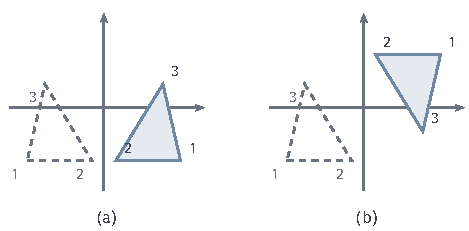
\includegraphics{figures/02-vectors-matrices-and-multivariate-calculus/03-linear-equations-and-optimization/tikz/learning-mechanisms/reflection-versus-rotation.pdf}
  \caption{反射与旋转的几何区别。虚线为原三角形，实色为变换后的位置；(a)关于纵轴反射，行列式为$-1$；(b)绕两轴交点旋转$180^\circ$，行列式为$1$。两幅图仅用于说明允许变换集合的不同，不表示给定矩阵的最优逼近结果。}
  \label{fig:solver-reflection-versus-rotation}
\end{figure}

\paragraph{$s=-1$时原来的上界取不到}
若$s=-1$，$\bm U\bm V^\top$不可行，需要新的上界。仍令$\bm Z=\bm U^\top\bm R\bm V$。对任一旋转$\bm R$，$\bm Z$正交，且
\[
 \det\bm Z=\det\bm U\cdot\det\bm R\cdot\det\bm V=s=-1 .
\]
上一小节的上界依赖$\bm Z=\bm I$可以取到；现在$\det\bm I=1$，这已不可能。

先看$d=2$。行列式为$-1$的二阶正交矩阵都形如
\[
 \bm Z=\begin{bmatrix}\cos\theta&\sin\theta\\\sin\theta&-\cos\theta\end{bmatrix},
\]
它是关于一条直线的反射。代入上一小节的目标，
\[
 \operatorname{tr}(\bm Z^\top\bm\Sigma)=\sigma_1\cos\theta-\sigma_2\cos\theta=(\sigma_1-\sigma_2)\cos\theta .
\]
由$\sigma_1\geq\sigma_2$，它在$\theta=0$处取最大值$\sigma_1-\sigma_2$，这时
\[
 \bm Z=\begin{bmatrix}1&0\\0&-1\end{bmatrix}.
\]
与无约束的上界$\sigma_1+\sigma_2$相比，迹少了$2\sigma_2$：两个对角元不能都取$1$，较小奇异值对应的那个对角元被迫取$-1$。这个例子中$\operatorname{tr}\bm Z=0=d-2$，下面的引理说明一般情形也如此。

\begin{lemma}[行列式为负的正交矩阵的迹]
\label{lem:matrix-approximation-reflection-trace}
设$\bm Z\in\mathbb R^{d\times d}$正交且$\det\bm Z=-1$，则存在单位向量$\bm x$使$\bm Z\bm x=-\bm x$，并且$\operatorname{tr}\bm Z\leq d-2$。
\end{lemma}
\begin{proof}
先证$-1$是特征值。由$\bm Z^\top\bm Z=\bm I$，
\[
 \bm Z+\bm I=\bm Z(\bm I+\bm Z^\top)=\bm Z(\bm I+\bm Z)^\top .
\]
取行列式得
\[
 \det(\bm Z+\bm I)=\det\bm Z\cdot\det(\bm I+\bm Z)=-\det(\bm Z+\bm I),
\]
所以$\det(\bm Z+\bm I)=0$，存在单位向量$\bm x$使$\bm Z\bm x=-\bm x$。再由
\[
 \bm x=\bm Z^\top\bm Z\bm x=-\bm Z^\top\bm x
\]
得$\bm Z^\top\bm x=-\bm x$。

$d=1$时$\bm Z=(-1)$，$\operatorname{tr}\bm Z=-1=d-2$。设$d\geq2$，把$\bm x$扩充为$\mathbb R^d$的标准正交基，排成正交矩阵$\bm Q=[\bm x,\bm Q_2]$。由$\bm Z\bm x=-\bm x$与$\bm Z^\top\bm x=-\bm x$，非对角块为零：
\[
 \bm Q_2^\top\bm Z\bm x=-\bm Q_2^\top\bm x=\bm0,\qquad
 \bm x^\top\bm Z\bm Q_2=(\bm Z^\top\bm x)^\top\bm Q_2=\bm0 .
\]
于是
\[
 \bm Q^\top\bm Z\bm Q=\begin{bmatrix}-1&\bm0\\\bm0&\bm Z_2\end{bmatrix},\qquad\bm Z_2=\bm Q_2^\top\bm Z\bm Q_2 .
\]
左端是正交矩阵的乘积，仍正交，所以$\bm Z_2$的各列是单位向量，对角元都不超过$1$，$\operatorname{tr}\bm Z_2\leq d-1$。迹在相似变换下不变，故
\[
 \operatorname{tr}\bm Z=-1+\operatorname{tr}\bm Z_2\leq d-2 .
\]
\end{proof}

用特征值的语言看，同一结论是这样的。实正交矩阵的特征值模都为$1$：非实特征值成共轭对出现，每对的乘积为$1$、实部之和不超过$2$；实特征值只能是$\pm1$。行列式等于全部特征值之积，为$-1$时特征值$-1$必出现奇数次，至少一次。迹等于特征值之和，于是至多为$(d-1)\cdot1+(-1)=d-2$。上面的证明只用实向量完成了同一论证。

\paragraph{修正最小奇异方向}
有了引理，就可以像$d=2$时那样估计迹的损失。把无约束上界与目标相减，
\[
 \sum_{i=1}^d\sigma_i-\operatorname{tr}(\bm Z^\top\bm\Sigma)=\sum_{i=1}^d\sigma_i(1-z_{i,i}).
\]
每个$1-z_{i,i}$都非负，由引理，它们的和是$d-\operatorname{tr}\bm Z\geq2$。损失是这些量以奇异值为权重的和，而每个权重都不小于最小奇异值$\sigma_d$，所以损失至少是
\[
 \sigma_d(d-\operatorname{tr}\bm Z)\geq2\sigma_d .
\]
这个下界在缺口全部集中于最后一个对角元时取到：$z_{d,d}=-1$，$1-z_{d,d}=2$，其余对角元都等于$1$。相应的$\bm Z$是
\begin{equation}
 \bm D_s=\operatorname{diag}(1,\ldots,1,s),
 \label{eq:matrix-approximation-rotation-correction}
\end{equation}
即只把最后一个对角元改为$s=-1$。换回原变量，最优旋转是$\bm R_\star=\bm U\bm D_s\bm V^\top$。$s=1$时$\bm D_s=\bm I$，这个公式也包含了行列式约束不起作用的情形。

\begin{theorem}[最佳旋转逼近]
\label{thm:matrix-approximation-best-rotation}
设$\bm A\in\mathbb R^{d\times d}$有SVD$\bm A=\bm U\bm\Sigma\bm V^\top$，$\sigma_1\geq\cdots\geq\sigma_d\geq0$，$s=\det(\bm U\bm V^\top)$，$\bm D_s=\operatorname{diag}(1,\ldots,1,s)$。则对一切满足$\bm R^\top\bm R=\bm I$、$\det\bm R=1$的$\bm R$，
\begin{equation}
 \operatorname{tr}(\bm R^\top\bm A)\leq\sum_{i=1}^{d-1}\sigma_i+s\,\sigma_d ,
 \label{eq:matrix-approximation-rotation-trace-bound}
\end{equation}
等号由$\bm R_\star=\bm U\bm D_s\bm V^\top$取到。因此
\begin{equation}
 \min_{\bm R^\top\bm R=\bm I,\ \det\bm R=1}\lVert\bm A-\bm R\rVert_{\mathrm F}^2
 =\sum_{i=1}^{d-1}(\sigma_i-1)^2+(\sigma_d-s)^2 .
 \label{eq:matrix-approximation-rotation-min-error}
\end{equation}
\end{theorem}
\begin{proof}
$\bm R_\star$是正交矩阵的乘积，仍正交，且$\det\bm R_\star=\det\bm U\cdot s\cdot\det\bm V=s^2=1$，所以它是旋转。

$s=1$时$\bm D_s=\bm I$，上界就是定理~\ref{thm:ls-best-orthogonal-approximation}对全部正交矩阵给出的$\sum_i\sigma_i$，在旋转中自然成立，且由$\bm R_\star=\bm U\bm V^\top$取到。

设$s=-1$。对任一旋转$\bm R$，令$\bm Z=\bm U^\top\bm R\bm V$，则$\det\bm Z=-1$，由引理~\ref{lem:matrix-approximation-reflection-trace}，$\operatorname{tr}\bm Z\leq d-2$。与上一小节相同，$\operatorname{tr}(\bm R^\top\bm A)=\sum_i\sigma_iz_{i,i}$。由$|z_{i,i}|\leq1$得$1-z_{i,i}\geq0$，又$\sigma_i\geq\sigma_d$，所以
\[
 \begin{aligned}
 \sum_{i=1}^d\sigma_i-\operatorname{tr}(\bm R^\top\bm A)
 &=\sum_{i=1}^d\sigma_i(1-z_{i,i})
 \geq\sigma_d\sum_{i=1}^d(1-z_{i,i})\\
 &=\sigma_d(d-\operatorname{tr}\bm Z)\geq2\sigma_d ,
 \end{aligned}
\]
即
\[
 \operatorname{tr}(\bm R^\top\bm A)\leq\sum_{i=1}^{d-1}\sigma_i-\sigma_d .
\]
$\bm R=\bm R_\star$时$\bm Z=\bm D_s$，迹恰为$\sum_{i<d}\sigma_i-\sigma_d$，等号成立。

最后代入展开式。由$\lVert\bm A\rVert_{\mathrm F}^2=\sum_i\sigma_i^2$与$s^2=1$，
\[
 \sum_{i=1}^d\sigma_i^2+d-2\Bigl(\sum_{i=1}^{d-1}\sigma_i+s\sigma_d\Bigr)
 =\sum_{i=1}^{d-1}(\sigma_i-1)^2+(\sigma_d-s)^2 .
\]
\end{proof}

\paragraph{修正的代价}
修正只发生在最小奇异方向上。$\bm R_\star=\bm U\bm D_s\bm V^\top$与无约束解$\bm U\bm V^\top$的差别，是把最后一对奇异方向的配对改为$\bm v_d\mapsto s\bm u_d$。若把符号改放在第$i$个方向上，同样得到旋转，但迹损失$2\sigma_i$；定理证明中的不等式说明，任何旋转的迹损失都至少是$2\sigma_d$，所以放在最小奇异方向上损失最少。

$s=-1$时，最小平方误差比无行列式约束时增加
\begin{equation}
 (\sigma_d+1)^2-(\sigma_d-1)^2=4\sigma_d .
 \label{eq:matrix-approximation-rotation-cost}
\end{equation}
$\bm A$可逆时，$\det\bm A=\det\bm U\det\bm\Sigma\det\bm V$且$\det\bm\Sigma>0$，所以$s$就是$\det\bm A$的符号，与所取的SVD无关：$\det\bm A>0$时约束不起作用，$\det\bm A<0$时代价为$4\sigma_d$。

$\sigma_d=0$时，$s$依赖SVD的选取：把$\bm u_d$换成$-\bm u_d$不改变$\bm A$，却改变$\det\bm U$的符号。但这时$(\sigma_d-s)^2=1$与$s$无关，旋转约束的代价为零。两种选取还给出同一个$\bm R_\star$，因为符号同时出现在$\bm u_d$与$s$中，乘积$s\bm u_d$不变。

\paragraph{唯一性}
唯一性分两种情形说明。第一种，$\bm A$可逆且$s=1$：无约束问题的唯一解$\bm W$本身是旋转，所以它也是旋转约束下的唯一解。

第二种，$\sigma_{d-1}>\sigma_d$。若$\sigma_d>0$且$s=-1$，定理证明中的不等式取等要求$(\sigma_i-\sigma_d)(1-z_{i,i})=0$，从而$i<d$时$z_{i,i}=1$，$\bm Z$的前$d-1$列是$\bm e_1,\ldots,\bm e_{d-1}$；最后一列只能是$\pm\bm e_d$，行列式为$-1$又迫使它为$-\bm e_d$，即$\bm Z=\bm D_s$。

若$\sigma_d=0$，先取使$s=1$的SVD，取等要求$z_{i,i}=1$（$i<d$），同理$\bm Z=\operatorname{diag}(1,\ldots,1,\pm1)$，而$\det\bm Z=s=1$，故$\bm Z=\bm I$。两种情况下最优旋转都唯一。

最小奇异值重复且$s=-1$，或$\operatorname{rank}\bm A\leq d-2$时，最优旋转可以不唯一，例子见本小节的算法分析。

\subsubsection{算法实现}

计算在上一小节的基础上增加两步：求出符号$s$，再在最小奇异方向上作修正。下面写出用到的变量与各步计算，并用以下示例逐步演示。

\begin{example}[对角矩阵的旋转逼近]
\label{ex:matrix-approximation-rotation-diagonal}
求离
\[
 \bm A=\begin{bmatrix}3&0\\0&-1\end{bmatrix}
\]
最近的旋转。$\det\bm A=-3<0$，上一小节的无约束解包含反射，行列式约束会起作用。下面的逐步执行给出$\bm R_\star$与平方误差，并与无约束解比较。
\end{example}

\paragraph{变量}
\begin{itemize}
 \item $\bm A\in\mathbb R^{d\times d}$：给定的方阵。
 \item $\bm U,\bm\Sigma,\bm V$：$\bm A$的完整方阵SVD，奇异值按非增顺序排列。
 \item $s=\det\bm U\det\bm V$：无约束解$\bm U\bm V^\top$的行列式。
 \item $\bm D_s=\operatorname{diag}(1,\ldots,1,s)$：最小奇异方向上的符号修正。
 \item $\bm R_\star$：所求的最优旋转。
\end{itemize}

\paragraph{输入与预处理}
输入方阵$\bm A$，预处理是求它的完整方阵SVD，并把奇异值按非增顺序排列，使最后一列$\bm u_d$、$\bm v_d$对应最小奇异值。符号修正要放在这一对方向上，排序不能省略。

例中
\[
 \bm A^\top\bm A=\begin{bmatrix}9&0\\0&1\end{bmatrix},
\]
可取$\bm V=\bm I$，奇异值$\sigma_1=3\geq\sigma_2=1$。由$\bm u_i=\bm A\bm v_i/\sigma_i$，
\[
 \bm u_1=\frac13\begin{bmatrix}3\\0\end{bmatrix}=\begin{bmatrix}1\\0\end{bmatrix},\qquad
 \bm u_2=\frac11\begin{bmatrix}0\\-1\end{bmatrix}=\begin{bmatrix}0\\-1\end{bmatrix},
\]
于是
\[
 \bm U=\begin{bmatrix}1&0\\0&-1\end{bmatrix},\qquad
 \bm\Sigma=\begin{bmatrix}3&0\\0&1\end{bmatrix},\qquad
 \bm V=\bm I ,
\]
核对$\bm U\bm\Sigma\bm V^\top=\operatorname{diag}(3,-1)=\bm A$。

\paragraph{计算步骤}
\begin{enumerate}
 \item \textbf{计算符号。}按式~\eqref{eq:matrix-approximation-rotation-sign}计算
 \[
  s=\det\bm U\det\bm V .
 \]
 例中
 \[
  s=(-1)\cdot1=-1 .
 \]
 作为对照，无约束的最优正交矩阵是$\bm U\bm V^\top=\operatorname{diag}(1,-1)$，它是关于横轴的反射，平方误差为
 \[
  \lVert\operatorname{diag}(2,0)\rVert_{\mathrm F}^2=4=(3-1)^2+(1-1)^2 .
 \]

 \item \textbf{构造修正矩阵。}按式~\eqref{eq:matrix-approximation-rotation-correction}取
 \[
  \bm D_s=\operatorname{diag}(1,\ldots,1,s).
 \]
 例中
 \[
  \bm D_s=\begin{bmatrix}1&0\\0&-1\end{bmatrix}.
 \]

 \item \textbf{相乘得最优旋转。}计算
 \begin{equation}
  \bm R_\star=\bm U\bm D_s\bm V^\top .
  \label{eq:matrix-approximation-rotation-optimum}
 \end{equation}
 例中
 \[
  \bm R_\star=\begin{bmatrix}1&0\\0&-1\end{bmatrix}\begin{bmatrix}1&0\\0&-1\end{bmatrix}=\begin{bmatrix}1&0\\0&1\end{bmatrix}.
 \]

 \item \textbf{核验。}同时检查三项：$\bm R_\star^\top\bm R_\star=\bm I$，$\det\bm R_\star=1$，误差平方等于$\sum_{i<d}(\sigma_i-1)^2+(\sigma_d-s)^2$。

 例中$\bm R_\star=\bm I$，前两项显然成立；残差为$\bm A-\bm R_\star=\operatorname{diag}(2,-2)$，
 \[
  \lVert\bm A-\bm R_\star\rVert_{\mathrm F}^2=4+4=8=(3-1)^2+(1+1)^2 .
 \]
 比无约束时多$4=4\sigma_2$。
\end{enumerate}

最终得到离$\bm A$最近的旋转
\[
 \bm R_\star=\begin{bmatrix}1&0\\0&1\end{bmatrix},
\]
平方误差为$8$。

二阶旋转可以全部写出来，用于独立核对。对
\[
 \bm R=\begin{bmatrix}\cos\theta&-\sin\theta\\\sin\theta&\cos\theta\end{bmatrix},
\]
按元素求和得
\[
 \operatorname{tr}(\bm R^\top\bm A)=3\cos\theta-\cos\theta=2\cos\theta ,
\]
它只在$\theta=0$处取最大值$2=\sigma_1-\sigma_2$。所以$\bm R_\star=\bm I$是唯一的最优旋转，与$\sigma_1>\sigma_2$时的唯一性一致。

\subsubsection{算法分析}

\paragraph{计算代价}
与无约束情形相比，额外的工作只是求两个正交矩阵的行列式与一次对角缩放，主要代价仍是SVD。是否需要修正完全由$s$决定，不必比较多个候选。

\paragraph{最优旋转不唯一的情形}
最小奇异值重复时，唯一性可能失败。取$\bm A=\operatorname{diag}(1,-1)$，奇异值为$1,1$，$s=-1$。对上面的任一二阶旋转，
\[
 \operatorname{tr}(\bm R^\top\bm A)=\cos\theta-\cos\theta=0 ,
\]
由展开式~\eqref{eq:matrix-approximation-orthogonal-expansion}，所有旋转的误差平方都是
\[
 \lVert\bm A\rVert_{\mathrm F}^2+2-0=4 ,
\]
与公式$(1-1)^2+(1+1)^2=4$一致，但最优旋转有无穷多个。

$\operatorname{rank}\bm A\leq d-2$时也有类似的自由度，例如$\bm A=\bm0$时每个旋转都最优。

\paragraph{接近奇异时的敏感性}
最小奇异值接近零时，$s$对$\bm A$的微小变化很敏感：$\det\bm A$接近零，它的符号可能被扰动改变，最优旋转随之跳到另一个。但对同一个$\bm A$，两种符号给出的误差平方恰好相差$4\sigma_d$，这时也很小，最优误差本身随$\bm A$连续变化。所以这种情形下应报告最优误差，而不应把所得的旋转当作稳定的估计。

% 第15章第6节：逼近结果的检验。

\section{逼近结果的检验}
\label{sec:matrix-approximation-verification}

前几节的最优解都由SVD读出，实际计算出的近似矩阵还要检验。检验回答三个问题：结果是否满足约束，残差是否达到理论下界，残差中哪一部分来自约束本身、哪一部分来自计算。三项检验都要用问题所规定的那一种误差范数；用别的范数评价，会把正确的结果误判为不好，或把不好的结果误判为可接受。

第一项是约束。低秩近似若以因子$\bm U_k$、$\bm\Sigma_k$、$\bm V_k$的形式保存，秩不超过$k$由因子形式直接保证；若已经乘成完整矩阵$\widehat{\bm X}$，可以看它第$k$个以后的奇异值是否只在舍入误差的量级。正交逼近与旋转逼近要检查$\lVert\widehat{\bm R}^\top\widehat{\bm R}-\bm I\rVert_{\mathrm F}$是否接近零；旋转还要检查$\det\widehat{\bm R}=1$，而不是$-1$。

第二项是残差与理论下界的比较。直接计算残差，再与本章给出的最优误差对照：秩$k$逼近在Frobenius范数下为$(\sum_{i>k}\sigma_i^2)^{1/2}$，在谱范数下为$\sigma_{k+1}$；可分离权重下为$(\sum_{i>k}\tilde\sigma_i^2)^{1/2}$；正交逼近的平方误差为$\sum_i(\sigma_i-1)^2$，旋转逼近再加上$s=-1$时的$4\sigma_d$。

满足约束的任何候选，残差都不会低于这些下界。所以若直接算出的残差明显低于下界，说明结果实际上违反了约束（例如数值秩大于$k$），或者所用的奇异值本身不准确；若明显高于下界，则说明计算或截断有误，例如奇异值没有按降序排列，或左右奇异向量的配对被打乱。加权问题要用加权残差比较：示例~\ref{ex:matrix-approximation-weighted-low-rank}中的$\bm X_1=\operatorname{diag}(0,2)$按普通Frobenius范数的误差为$3$，比直接截断$\bm A$的误差$2$大，但它在加权意义下才是最优的。

第三项是区分两种误差。逼近误差由约束决定：秩预算或正交性使$\bm A$本身不可行时，即使精确计算，残差也等于理论下界而不为零，这部分不能靠提高计算精度消除。计算误差则是计算结果与精确最优解之间的差别，来自SVD等步骤的舍入，表现为直接残差与理论下界之间的差距，以及约束检验中偏离零的量。

两者对扰动的反应也不同。由第~\ref{chap:condition-and-spectral-perturbation}章奇异值的Weyl界（定理~\ref{thm:ls-weyl-singular-value}），$\bm A$受到谱范数不超过$\varepsilon$的扰动时，每个奇异值的变化不超过$\varepsilon$，所以最优误差$\sigma_{k+1}$的数值是稳定的。取得最优误差的矩阵却依赖奇异子空间：间隙$\sigma_k-\sigma_{k+1}$很小时，前$k$个奇异方向可能明显转动；间隙为零时，第~\ref{sec:matrix-approximation-low-rank-uniqueness}节已经说明最优矩阵本身不唯一。因此间隙很小时，应把最优误差当作可靠的结论，而把具体的近似矩阵当作许多近乎同样好的候选之一。

本章的算例可以按这三项核对。示例~\ref{ex:matrix-approximation-truncated-three-by-three}中$\bm A_1$秩为一，直接算出的残差为$\sqrt2$（Frobenius）与$1$（谱范数），分别等于$(\sigma_2^2+\sigma_3^2)^{1/2}$与$\sigma_2$；示例~\ref{ex:matrix-approximation-orthogonal-two-by-two}中$\bm R_\star^\top\bm R_\star=\bm I$，平方误差$5=(3-1)^2+(2-1)^2$；示例~\ref{ex:matrix-approximation-rotation-diagonal}中$\det\bm R_\star=1$，平方误差$8=4+4\sigma_2$。这些都是精确算例，计算误差为零，残差全部来自约束。

最后区分本章的截断与第~\ref{chap:solution-error-regularization}章的截断。那里的截断SVD求解$\bm x_k=\bm A_k^\dagger\bm b$同样只保留前$k$个奇异方向，但目的是从带误差的观测中稳定地求出输入，检验的是向量残差$\bm b-\bm A\bm x_k$与解的误差；选择$k$时，要同时比较舍弃方向带来的拟合损失与保留方向上$1/\sigma_k$的噪声放大。本章检验的是矩阵残差$\bm A-\bm A_k$，最佳矩阵逼近本身不替代那里对$k$的判断。

\FloatBarrier
\section{本章小结}
\label{sec:matrix-approximation-summary}

本章开头的问题是：给定矩阵$\bm A$，在秩约束或正交约束下，哪一个矩阵离它最近，最小误差是多少，最优矩阵是否唯一。各节的解法遵循同一条路线：先写清约束与误差；再固定一个表示，在其中选出最优系数；最后选择表示本身，即方向、子空间或正交因子。前两步把矩阵优化化成向量的投影与特征值比较，SVD则把最优解写成具体的矩阵。

秩一逼近中，固定单位方向$\bm u$时，最优系数是投影系数$\bm c=\bm A^\top\bm u$，误差等于$\lVert\bm A\rVert_{\mathrm F}^2$减去保留量$\bm u^\top\bm A\bm A^\top\bm u$。选方向就是最大化Rayleigh商。对任意实对称$\bm S$，Rayleigh商介于最小、最大特征值之间，取等的方向恰是相应特征空间中的非零向量。用到$\bm A\bm A^\top$上，最优秩一近似为$\sigma_1\bm u_1\bm v_1^\top$，平方误差为$\sum_{i\geq2}\sigma_i^2$；它在$\sigma_1>\sigma_2$时唯一，奇异向量同时变号只改变写法。

秩$k$逼近中，固定子空间的最优重建是正交投影，选子空间化为迹极值：$k$维子空间上的迹不超过前$k$个特征值之和。由此得到Eckart--Young--Mirsky定理：截断SVD$\bm A_k$在全部秩不超过$k$的矩阵中同时使Frobenius误差与谱范数误差最小，最小值分别为$(\sum_{i>k}\sigma_i^2)^{1/2}$与$\sigma_{k+1}$。Frobenius最优解在$\sigma_k>\sigma_{k+1}$时唯一；谱范数最优解即使有间隙也一般不唯一。这些结论只对全部秩不超过$k$的矩阵与这两种范数成立，额外的非负、稀疏约束或一般的逐元素权重都会使截断SVD失去最优性。

改用加权长度规定单位方向时，Rayleigh商推广为广义Rayleigh商。$\bm B$正定时，用Gram因子换元可化为普通Rayleigh商，极值是广义特征值，广义特征向量可以选成$\bm B$正交；计算用Cholesky分解与三角求解保持对称结构，不应改求一般不对称的$\bm B^{-1}\bm S$。$\bm B$不正定时这一化归失效。

误差的权重能分离为行权重与列权重时，加权低秩逼近经可逆变换化为普通低秩逼近，最优解由变换后矩阵的截断SVD还原，最佳方向正是一个广义Rayleigh商的最大特征向量。这一化归要求逐元素权重是行因子与列因子的乘积；任意权重与缺失元素没有截断SVD式的闭式解，交由卷五的优化方法处理。

正交约束下，距离最小化成迹最大化，目标关于未知矩阵是线性的。最优正交矩阵是$\bm U\bm V^\top$，即第~\ref{chap:polar-decomposition}章极分解的正交因子，平方误差为$\sum_i(\sigma_i-1)^2$；$\bm A$可逆时它唯一，奇异时自由度只在零奇异值方向上。要求旋转时，只需在最小奇异方向上作符号修正，$\bm R_\star=\bm U\operatorname{diag}(1,\ldots,1,\det(\bm U\bm V^\top))\bm V^\top$；$\det(\bm U\bm V^\top)=-1$时误差平方增加$4\sigma_d$，$\sigma_d=0$时修正不增加误差。

在这些问题中，Rayleigh商、迹极值与截断SVD承担的是最优性工具的职责：它们说明为什么由SVD读出的矩阵最好，以及在什么条件下唯一。计算出的结果要按同一种误差范数检验约束与残差，把约束带来的逼近误差与计算误差分开；最优误差的数值对扰动稳定，最优矩阵在间隙小时则不稳定。本章的截断矩阵用于重建$\bm A$本身，与第~\ref{chap:solution-error-regularization}章为稳定求解方程而截断取逆的用途不同；不能化归到SVD的一般逼近问题，则由卷五的迭代优化展开。


\chapter{矩阵方程}
\label{chap:matrix-equations}

前面各章的未知量都是向量。有些问题的未知量却是一整张矩阵$\bm X$，而且它同时受到已知矩阵的左乘和右乘。第~\ref{chap:condition-and-spectral-perturbation}章证明谱隙界时已经遇到这样的方程：未知矩阵左边乘一个对角矩阵、右边乘另一个，两项相减等于已知矩阵。第~\ref{chap:linear-recurrence-stability}章的递推$\bm x_{k+1}=\bm A\bm x_k$也提出类似的问题：若每一步以二次量计量状态，全部步骤的累计量能否由一个矩阵直接写出？这个矩阵满足的同样是一个左右两侧都有$\bm A$作用的方程。

本章回答三个问题：这类方程何时对任意右端都唯一可解；怎样在不形成巨大系数矩阵的前提下算出解；对称右端的Lyapunov方程，解何时对称、何时正定，正定解又能证明什么。

第~\ref{sec:ls-matrix-equations}节研究Sylvester方程$\bm A\bm X+\bm X\bm B=\bm C$。向量化说明它是矩阵空间上的线性方程，可解性由两侧系数的特征值之和决定；计算则用第~\ref{chap:eigen-spectral-decomposition}章的实Schur形把两个系数化为准三角形，再像第~\ref{chap:direct-linear-solvers}章的三角回代那样逐块求解。可对角化时换到特征基更简单，但特征基不正交时误差会被放大。

第~\ref{sec:ls-lyapunov}节由离散累计引出Lyapunov方程，并把连续型方程作为Sylvester方程的特例。两类方程只需一次Schur分解，就能保持对称结构逐元素递推。离散型的正定解由第~\ref{chap:linear-recurrence-stability}章的矩阵幂几何上界和绝对收敛级数构造；连续型正定解的积分证明要用矩阵指数，留给后续关于演化的理论，本章只陈述条件并给出代数检验。

全章用$\bm X$表示未知矩阵，Lyapunov方程统一写成离散型$\bm X-\bm A^\top\bm X\bm A=\bm Q$与连续型$\bm A^\top\bm X+\bm X\bm A=-\bm Q$。无论哪种算法，最后都在原方程中计算残差，以它检验整个流程；Schur路线的正交变换保证这个残差与变换后坐标中的残差相同。

% 矩阵方程（一）：Sylvester方程AX+XB=C（线性算子表示与向量化、可解性与谱分离条件、Schur分解法、特征基下的求解）

\section{Sylvester方程}
\label{sec:ls-matrix-equations}

本节研究未知矩阵同时受左乘和右乘的Sylvester方程。先说明它是矩阵空间上的线性方程，再由两侧系数的特征值给出存在唯一性条件；计算时用正交Schur变换把方程化为准三角形后逐块回代，可对角化的系数还可以换到特征基逐元素相除。两条计算路线都不形成巨大的Kronecker系数矩阵。

\subsection{矩阵方程的线性算子表示}
\label{sec:ls-matrix-equation-types}

已知矩阵从左边、右边或两边作用在未知矩阵上，这样的方程称为\term{矩阵方程}（matrix equation）。最简单的是单侧方程$\bm A\bm X=\bm C$：$\bm X$的每一列分别满足一个以$\bm A$为系数的线性方程，所以它就是共用系数的多右端线性方程。双侧方程$\bm A\bm X\bm B=\bm C$中，$\bm A$作用在$\bm X$的列上，$\bm B$作用在$\bm X$的行上；两侧系数可逆时，可以先左乘$\bm A^{-1}$、再右乘$\bm B^{-1}$，两次“除法”互不干扰。

本节研究左右两种作用相加的\term{Sylvester方程}（Sylvester equation）
\begin{equation}
 \bm A\bm X+\bm X\bm B=\bm C,
 \label{eq:ls-sylvester-equation}
\end{equation}
其中$\bm A\in\mathbb R^{m\times m}$、$\bm B\in\mathbb R^{d\times d}$、$\bm C\in\mathbb R^{m\times d}$，未知量$\bm X\in\mathbb R^{m\times d}$。$\bm A$作用在$\bm X$的列上，阶数等于$\bm X$的行数；$\bm B$作用在$\bm X$的行上，阶数等于$\bm X$的列数。

两项相加以后，就不能分别“除以”两个系数。即使$\bm A$可逆，左乘$\bm A^{-1}$也只得到$\bm X+\bm A^{-1}\bm X\bm B=\bm A^{-1}\bm C$，未知量仍同时出现在两项中。所以必须把左边整体看作一个作用在$\bm X$上的映射。

记$\mathcal L(\bm X)=\bm A\bm X+\bm X\bm B$。由矩阵乘法的分配律，$\mathcal L$对$\bm X$是线性的，所以Sylvester方程就是$md$维空间$\mathbb R^{m\times d}$上的线性方程$\mathcal L(\bm X)=\bm C$。

为了写出它的系数矩阵，把矩阵按列拉直，并使用第~\ref{sec:ls-kronecker-products}节的恒等式
\[
 \operatorname{vec}(\bm A\bm X\bm B)=(\bm B^\top\otimes\bm A)\operatorname{vec}\bm X .
\]
把$\bm A\bm X$看成$\bm A\bm X\bm I_d$、把$\bm X\bm B$看成$\bm I_m\bm X\bm B$，相加得
\begin{equation}
 (\bm I_d\otimes\bm A+\bm B^\top\otimes\bm I_m)\operatorname{vec}\bm X
 =\operatorname{vec}\bm C .
 \label{eq:ls-sylvester-vectorized}
\end{equation}

记系数矩阵为$\bm K\in\mathbb R^{md\times md}$。这一表达说明，前面关于线性方程的判据都适用于Sylvester方程；对小例子，也可以直接用LU分解（第~\ref{sec:ls-lu}节）求解式~\eqref{eq:ls-sylvester-vectorized}来核验。但$\bm K$有$(md)^2$个元素，$m=d=100$时已达$10^8$个，稠密消元约需$\tfrac23(md)^3$次运算。所以向量化只用来理解线性结构和判断可解性，大规模求解应保留矩阵形状。

\subsection{可解性与唯一性条件}
\label{sec:ls-matrix-equation-existence}

单侧方程可以直接沿用列空间判据：$\bm A\bm X=\bm C$相容，当且仅当$\bm C$的每一列都在$\operatorname{range}(\bm A)$中，即$\operatorname{rank}[\bm A\ \bm C]=\operatorname{rank}(\bm A)$。双侧方程的相容性由向量化方程$(\bm B^\top\otimes\bm A)\operatorname{vec}\bm X=\operatorname{vec}\bm C$的增广秩判据判断。两侧系数都可逆时，唯一解为$\bm X=\bm A^{-1}\bm C\bm B^{-1}$；任一侧秩亏时，方程可能无解，有解时解也可以沿该侧的零空间变动，因而不唯一。

Sylvester方程不能这样逐侧处理，对角情形能看出原因。设$\bm A=\operatorname{diag}(\lambda_1,\ldots,\lambda_m)$、$\bm B=\operatorname{diag}(\mu_1,\ldots,\mu_d)$，则$\bm A\bm X$把第$i$行乘以$\lambda_i$，$\bm X\bm B$把第$j$列乘以$\mu_j$。于是方程按元素分解为
\[
 (\lambda_i+\mu_j)\,x_{i,j}=c_{i,j},
\]
分母非零时
\begin{equation}
 x_{i,j}=\frac{c_{i,j}}{\lambda_i+\mu_j}.
 \label{eq:ls-sylvester-diagonal-closed-form}
\end{equation}

若某个$\lambda_i+\mu_j=0$，该位置退化为$0\cdot x_{i,j}=c_{i,j}$：$c_{i,j}\neq0$时无解，$c_{i,j}=0$时$x_{i,j}$可以任取。所以决定可解性的，是$\bm A$的特征值与$-\bm B$的特征值是否重合（图~\ref{fig:ls-sylvester-separation}），而不是两侧系数各自是否可逆。一般情形的结论相同，只是实矩阵的特征值可能是复数，条件要在复数域中检查。下面记$\operatorname{spec}(\bm A)$为$\bm A$在复数域中的全体特征值。

\begin{figure}[htbp]
  \centering
  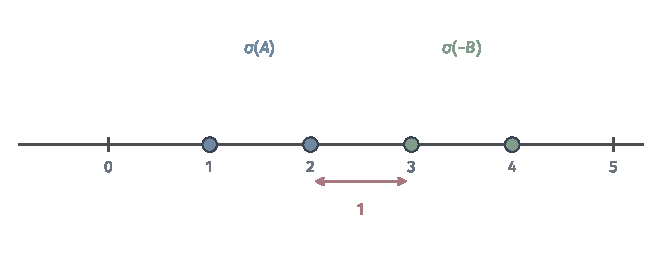
\includegraphics[width=112mm]{figures/00-shared/mathematical-preliminaries-upper/02-linear-spaces/matplotlib/ls-sylvester-separation/ls-sylvester-separation.pdf}
  \caption{谱分离条件的实轴示意。$\bm A=\operatorname{diag}(1,2)$的特征值$\{1,2\}$与$-\bm B$（$\bm B=\operatorname{diag}(-3,-4)$）的特征值$\{3,4\}$不相交，最近一对相距$1$，所以四个分母$\lambda_i+\mu_j$都不为零，对任意$\bm C$方程都有唯一解。}
  \label{fig:ls-sylvester-separation}
\end{figure}

\begin{theorem}[Sylvester方程的唯一可解性]
\label{thm:ls-sylvester-unique-solvability}
设$\bm A\in\mathbb R^{m\times m}$、$\bm B\in\mathbb R^{d\times d}$。方程$\bm A\bm X+\bm X\bm B=\bm C$对每个$\bm C\in\mathbb R^{m\times d}$都有唯一解，当且仅当
\begin{equation}
 \operatorname{spec}(\bm A)\cap\operatorname{spec}(-\bm B)=\varnothing ,
 \label{eq:ls-sylvester-spectral-separation}
\end{equation}
即对$\bm A$的任一特征值$\lambda$与$\bm B$的任一特征值$\mu$，都有$\lambda+\mu\neq0$。
\end{theorem}

\begin{proof}
$\mathcal L$把$\mathbb R^{m\times d}$映到自身。由秩零度定理，它对每个右端唯一可解，当且仅当齐次方程只有零解，也就是$\det\bm K\neq0$。这个行列式在实数域和复数域中是同一个数，所以可以在复数域中讨论齐次方程。

必要性。设$\bm A\bm u=\lambda\bm u$，且$-\lambda$是$\bm B$的特征值。$\bm B^\top$与$\bm B$有相同的特征多项式，所以$-\lambda$也是$\bm B^\top$的特征值，可取$\bm B^\top\bm w=-\lambda\bm w$，其中$\bm u,\bm w\neq\bm0$。于是$\bm X=\bm u\bm w^\top\neq\bm0$满足
\[
 \bm A\bm X+\bm X\bm B=\lambda\bm u\bm w^\top+\bm u(\bm B^\top\bm w)^\top=\lambda\bm u\bm w^\top-\lambda\bm u\bm w^\top=\bm0 ,
\]
齐次方程有非零解。

充分性。设$\bm A\bm X+\bm X\bm B=\bm0$，即$\bm A\bm X=\bm X(-\bm B)$。归纳得$\bm A^k\bm X=\bm X(-\bm B)^k$，从而对任意多项式$p$有
\[
 p(\bm A)\bm X=\bm X\,p(-\bm B) .
\]
取$p(z)=\prod_k(z-\lambda_k)$为$\bm A$的特征多项式，由Cayley--Hamilton定理~\ref{thm:ls-cayley-hamilton}，$p(\bm A)=\bm0$。另一方面，$p(-\bm B)=\prod_k(-\bm B-\lambda_k\bm I)$中每个$\lambda_k$都不是$-\bm B$的特征值，各因子可逆，所以$p(-\bm B)$可逆。于是$\bm X\,p(-\bm B)=\bm0$推出$\bm X=\bm0$。
\end{proof}

这一条件与$\bm A$、$\bm B$各自是否可逆无关。$\bm A=\bm0$、$\bm B=\bm I_d$时$\bm A$不可逆，方程却化为$\bm X=\bm C$，唯一可解；$1\times1$情形$\bm A=2$、$\bm B=-2$都可逆，方程却是$0\cdot x=c$。

谱不相交只回答解是否唯一，不回答解对数据误差是否敏感。对角情形下，最小的$|\lambda_i+\mu_j|$越接近零，$\bm C$的误差被放大得越多；矩阵远离正规时，即使所有谱和都远离零，解仍可能很敏感，第~\ref{sec:ls-sylvester-diagonalizable}节会看到其中的原因。

\subsection{Schur分解法}
\label{sec:ls-sylvester-schur}

稠密的一般Sylvester方程通常用\term{Bartels--Stewart算法}（Bartels--Stewart algorithm）求解。它的思路与解三角方程组相同：先用正交相似把两个系数化为准上三角形，未知元之间就有了先后依赖，可以逐个回代。下面设谱条件~\eqref{eq:ls-sylvester-spectral-separation}成立，依次说明变换、回代次序和二阶块的处理，再给出算法步骤、算例与分析。

\paragraph{主要思想：正交变换到准三角形}
第一步，分别对两个系数作实Schur分解（定理~\ref{thm:ls-real-schur}）
\[
 \bm A=\bm U\bm T\bm U^\top,\qquad \bm B=\bm V\bm S\bm V^\top,
\]
其中$\bm U,\bm V$正交，$\bm T,\bm S$是准上三角矩阵，对角块为$1\times1$（实特征值）或$2\times2$（一对共轭复特征值）。这一步只依赖$\bm A$、$\bm B$，与右端无关。

把分解代入$\bm A\bm X+\bm X\bm B=\bm C$，得
\[
 \bm U\bm T\bm U^\top\bm X+\bm X\bm V\bm S\bm V^\top=\bm C .
\]
两边左乘$\bm U^\top$、右乘$\bm V$，利用$\bm U^\top\bm U=\bm I$、$\bm V^\top\bm V=\bm I$，并记$\bm Y=\bm U^\top\bm X\bm V$、$\bm D=\bm U^\top\bm C\bm V$，方程化为
\begin{equation}
 \bm T\bm Y+\bm Y\bm S=\bm D .
 \label{eq:ls-sylvester-transformed}
\end{equation}
$\bm T$与$\bm A$、$\bm S$与$\bm B$分别相似，特征值相同，所以新方程同样满足谱条件。正交变换还不改变Frobenius范数：任一近似解$\bm Z$在原坐标中的残差，等于$\bm W=\bm U^\top\bm Z\bm V$在新坐标中的残差（下面定理~\ref{thm:ls-bartels-stewart}的第三条）。因此在新坐标中解得准确，换回原坐标后残差不会被放大。

\paragraph{主要思想：上三角情形的回代次序}
先看$\bm T$、$\bm S$都是上三角的情形。比较式~\eqref{eq:ls-sylvester-transformed}两边的$(i,j)$元，其中
\[
 (\bm T\bm Y)_{i,j}=\sum_{k\geq i}t_{i,k}y_{k,j},\qquad
 (\bm Y\bm S)_{i,j}=\sum_{\ell\leq j}y_{i,\ell}s_{\ell,j}.
\]
把含$y_{i,j}$的两项留在左边，得
\begin{equation}
 (t_{i,i}+s_{j,j})\,y_{i,j}
 =d_{i,j}-\sum_{k>i}t_{i,k}y_{k,j}-\sum_{\ell<j}y_{i,\ell}s_{\ell,j}.
 \label{eq:ls-sylvester-triangular-entry}
\end{equation}
右端第一个和只用同一列中更靠下的元素，第二个和只用同一行中更靠左的元素。所以按列$j=1,\ldots,d$从左向右，每列内按行$i=m,\ldots,1$从下向上计算，每一步右端都已知。除数$t_{i,i}+s_{j,j}$是$\bm A$与$\bm B$的一对特征值之和，由谱条件不为零。

同一次序也可以按整列写出。$\bm Y\bm S$的第$j$列是$\sum_{\ell\leq j}s_{\ell,j}\bm y_\ell$，比较式~\eqref{eq:ls-sylvester-transformed}两边的第$j$列，得
\begin{equation}
 (\bm T+s_{j,j}\bm I_m)\bm y_j=\bm d_j-\sum_{\ell<j}s_{\ell,j}\bm y_\ell .
 \label{eq:ls-sylvester-column-recursion}
\end{equation}
右端只用到更靠左的列；每列的系数是上三角矩阵，用第~\ref{sec:ls-lu}节的回代从最后一行向上求解，逐行展开正是式~\eqref{eq:ls-sylvester-triangular-entry}。图~\ref{fig:ls-bartels-stewart-column-order}画出了第$j$列的依赖：$\bm S$第$j$列中对角线以上的元素把已求出的列带进右端，对角元$s_{j,j}$并入当前列的三角系数。

\begin{figure}[htbp]
  \centering
  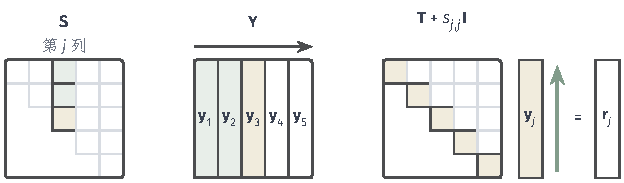
\includegraphics[width=109.6mm]{figures/01-basic-mathematics/03-vectors-matrices-and-multivariate-functions/tikz/c5-bartels-stewart-column-order/figure.pdf}
  \caption{Bartels--Stewart算法逐列求解$\bm T\bm Y+\bm Y\bm S=\bm D$的次序（上三角情形，图中取当前列$j=3$）。左：$\bm S$的第$j$列，绿色元素$s_{\ell,j}$（$\ell<j$）对应已求出的列，黄色为$s_{j,j}$。中：$\bm Y$的列从左到右求出。右：当前列解一个对角元为$t_{i,i}+s_{j,j}$的上三角方程组，从最后一行向上回代。}
  \label{fig:ls-bartels-stewart-column-order}
\end{figure}

\paragraph{主要思想：二阶对角块的局部系统}
实Schur形含$2\times2$对角块时，把一个标量未知数换成一个未知子块。按$\bm T$、$\bm S$的对角块把$\bm Y$、$\bm D$分块，记$\bm T$的第$I$个对角块为$\bm T_{I,I}$、$\bm S$的第$J$个对角块为$\bm S_{J,J}$，比较第$(I,J)$块得
\begin{equation}
 \begin{aligned}
 \bm T_{I,I}\bm Y_{I,J}+\bm Y_{I,J}\bm S_{J,J}
 &=\bm D_{I,J}-\sum_{K>I}\bm T_{I,K}\bm Y_{K,J}\\
 &\quad-\sum_{L<J}\bm Y_{I,L}\bm S_{L,J}.
 \end{aligned}
 \label{eq:ls-sylvester-block-recursion}
\end{equation}
右端只含同一块列中更靠下的块和更靠左的块列，因此按块列从左到右、每块列从下到上计算。

左边是一个小Sylvester方程，$\bm Y_{I,J}$至多是$2\times2$的，至多含四个未知数。由式~\eqref{eq:ls-sylvester-vectorized}，它的向量化系数是$\bm I\otimes\bm T_{I,I}+\bm S_{J,J}^\top\otimes\bm I$，至多为$4$阶，直接消元即可；只在这样的局部形成Kronecker系数。$\bm T_{I,I}$的特征值是$\bm A$的特征值，$\bm S_{J,J}$的特征值是$\bm B$的特征值，所以局部方程满足谱条件，由定理~\ref{thm:ls-sylvester-unique-solvability}唯一可解。

\paragraph{算法实现}
把上面三步连起来，Bartels--Stewart算法如下。
\begin{enumerate}
 \item 计算实Schur分解$\bm A=\bm U\bm T\bm U^\top$、$\bm B=\bm V\bm S\bm V^\top$，并变换右端$\bm D=\bm U^\top\bm C\bm V$。
 \item 按块列从左到右、每块列从下到上的次序，对每个块$(I,J)$从$\bm D_{I,J}$中减去已求出块的贡献，再解至多四个未知数的局部方程，得$\bm Y_{I,J}$。
 \item 恢复原未知量$\bm X=\bm U\bm Y\bm V^\top$，并在原方程中计算残差$\bm A\bm X+\bm X\bm B-\bm C$。精确算术下它为零；浮点计算中它的Frobenius范数与新坐标中的残差相同，可以直接用来检验整个流程。
\end{enumerate}
局部方程的系数接近奇异时，除法会放大误差，中间量也可能溢出。数值软件库中的实现因此常引入一个缩放因子$\sigma\in(0,1]$，实际求解$\bm T\bm Y+\bm Y\bm S=\sigma\bm D$，再连同$\sigma$一起返回，并对过小的局部分母给出警告。使用者应把$\sigma<1$或这类警告视为方程接近不可解的信号，而不是忽略它。

\begin{example}[Schur形方程的逐元素回代]
\label{ex:ls-sylvester-schur-form-entries}
先跳过Schur分解，直接从已为Schur形的系数出发，看逐元素回代应按什么次序进行。两个系数取为上三角矩阵
\[
 \bm T=\begin{bmatrix}1&2\\0&3\end{bmatrix},\qquad
 \bm S=\begin{bmatrix}4&1\\0&5\end{bmatrix},
\]
右端取为
\[
 \bm D=\begin{bmatrix}11&21\\21&35\end{bmatrix}.
\]
谱和$t_{i,i}+s_{j,j}$为$5,6,7,8$，都不为零，每个局部方程都可以相除。按式~\eqref{eq:ls-sylvester-triangular-entry}，第$1$列从下向上：
\[
 y_{2,1}=\frac{21}{3+4}=3,\qquad
 y_{1,1}=\frac{11-t_{1,2}y_{2,1}}{1+4}=\frac{11-2\cdot3}{5}=1 .
\]
第$2$列从下向上，右端还要减去左边一列经$s_{1,2}=1$带来的贡献：
\[
 \begin{aligned}
 y_{2,2}&=\frac{35-y_{2,1}s_{1,2}}{3+5}=\frac{35-3}{8}=4,\\
 y_{1,2}&=\frac{21-t_{1,2}y_{2,2}-y_{1,1}s_{1,2}}{1+5}=\frac{21-8-1}{6}=2 .
 \end{aligned}
\]
于是
\[
 \bm Y=\begin{bmatrix}1&2\\3&4\end{bmatrix}.
\]

代回检查全部四个元素：
\[
 \bm T\bm Y+\bm Y\bm S
 =\begin{bmatrix}7&10\\9&12\end{bmatrix}+\begin{bmatrix}4&11\\12&23\end{bmatrix}
 =\begin{bmatrix}11&21\\21&35\end{bmatrix}=\bm D .
\]
若次序颠倒，例如先算$y_{1,1}$，它的右端需要尚未求出的$y_{2,1}$，回代无法进行。
\end{example}

上例跳过了Schur分解。下面的例子从一般系数出发，完整走一遍变换、回代和恢复。

\begin{example}[Bartels--Stewart求解一个二阶方程]
\label{ex:ls-bartels-stewart-2x2}
系数取为
\[
 \bm A=\begin{bmatrix}-2&3\\-4&5\end{bmatrix},\qquad
 \bm B=\begin{bmatrix}1&1\\0&3\end{bmatrix},
\]
右端取为
\[
 \bm C=\begin{bmatrix}1&12\\-2&21\end{bmatrix}.
\]
$\bm A$的特征值为$2,1$，$-\bm B$的特征值为$-1,-3$，谱条件成立。

先作实Schur分解。由$\bm A(3,4)^\top=2(3,4)^\top$取
\[
 \bm U=\frac15\begin{bmatrix}3&-4\\4&3\end{bmatrix},\qquad
 \bm T=\bm U^\top\bm A\bm U=\begin{bmatrix}2&7\\0&1\end{bmatrix};
\]
$\bm B$已是上三角，取$\bm V=\bm I$、$\bm S=\bm B$。变换右端得
\[
 \bm D=\bm U^\top\bm C=\begin{bmatrix}-1&24\\-2&3\end{bmatrix}.
\]

在Schur坐标下逐列求解。第$1$列解$(\bm T+s_{1,1}\bm I)\bm y_1=\bm d_1$，即
\[
 \begin{bmatrix}3&7\\0&2\end{bmatrix}\bm y_1=\begin{bmatrix}-1\\-2\end{bmatrix},
\]
从下往上得$y_{2,1}=-1$、$y_{1,1}=2$。第$2$列的右端为
\[
 \bm d_2-s_{1,2}\bm y_1=(24,3)^\top-(2,-1)^\top=(22,4)^\top ,
\]
解
\[
 \begin{bmatrix}5&7\\0&4\end{bmatrix}\bm y_2=\begin{bmatrix}22\\4\end{bmatrix}
\]
得$y_{2,2}=1$、$y_{1,2}=3$。

变回原坐标，
\[
 \bm X=\bm U\bm Y=\frac15\begin{bmatrix}3&-4\\4&3\end{bmatrix}\begin{bmatrix}2&3\\-1&1\end{bmatrix}=\begin{bmatrix}2&1\\1&3\end{bmatrix}.
\]
核验：
\[
 \bm A\bm X+\bm X\bm B
 =\begin{bmatrix}-1&7\\-3&11\end{bmatrix}+\begin{bmatrix}2&5\\1&10\end{bmatrix}
 =\begin{bmatrix}1&12\\-2&21\end{bmatrix}=\bm C ,
\]
原方程残差为零。
\end{example}

\paragraph{算法分析：正确性}
上面的推导说明每一步都能进行，而且按次序算出的块满足各自的块等式。把这些事实合在一起，就得到算法的正确性和残差检验的依据。

\begin{theorem}[Bartels--Stewart算法的正确性]
\label{thm:ls-bartels-stewart}
设$\bm A=\bm U\bm T\bm U^\top$、$\bm B=\bm V\bm S\bm V^\top$是实Schur分解，谱条件~\eqref{eq:ls-sylvester-spectral-separation}成立，$\bm D=\bm U^\top\bm C\bm V$。则
\begin{enumerate}
 \item 按块列从左到右、每块列从下到上的次序，每一步的局部方程$\bm T_{I,I}\bm Y_{I,J}+\bm Y_{I,J}\bm S_{J,J}=\bm E_{I,J}$都唯一可解，其中右端$\bm E_{I,J}$由已求出的块给出；
 \item 由此算出的$\bm Y$是方程~\eqref{eq:ls-sylvester-transformed}的唯一解，$\bm X=\bm U\bm Y\bm V^\top$是$\bm A\bm X+\bm X\bm B=\bm C$的唯一解；
 \item 对任意$\bm Z\in\mathbb R^{m\times d}$，记$\bm W=\bm U^\top\bm Z\bm V$，有$\lVert\bm A\bm Z+\bm Z\bm B-\bm C\rVert_{\mathrm F}=\lVert\bm T\bm W+\bm W\bm S-\bm D\rVert_{\mathrm F}$。
\end{enumerate}
\end{theorem}

\begin{proof}
先证第三条。由$\bm A=\bm U\bm T\bm U^\top$、$\bm B=\bm V\bm S\bm V^\top$与$\bm Z=\bm U\bm W\bm V^\top$，
\[
 \bm A\bm Z+\bm Z\bm B-\bm C=\bm U(\bm T\bm W+\bm W\bm S-\bm D)\bm V^\top,
\]
而左右乘正交矩阵不改变Frobenius范数。

再证第一条。准上三角矩阵的特征值是各对角块特征值的并，$\bm T$与$\bm A$相似，所以$\bm T_{I,I}$的特征值都是$\bm A$的特征值；同理$\bm S_{J,J}$的特征值都是$\bm B$的特征值。于是每个局部方程满足谱条件，由定理~\ref{thm:ls-sylvester-unique-solvability}唯一可解。

最后证第二条。第$(I,J)$块等式的右端只含按次序已算出的块，所以算出的每一块都满足相应的块等式；全部块等式合起来就是式~\eqref{eq:ls-sylvester-transformed}。$\bm T$、$\bm S$满足谱条件，由定理~\ref{thm:ls-sylvester-unique-solvability}，这个解唯一。在第三条中取$\bm Z=\bm X$、$\bm W=\bm Y$，得原方程残差为零；原方程的唯一性同样由该定理给出。
\end{proof}

\paragraph{算法分析：计算代价}
实Schur分解靠迭代算出，常用实现计入正交因子约需$25m^3$与$25d^3$次运算\scite{math-golub2013matrix}。变换右端与变回原坐标各约$2(m^2d+md^2)$次，逐块回代约$m^2d+md^2$次；存储只需$O(m^2+d^2+md)$个数。$m=d=100$时总量约$6\times10^7$次，而对式~\eqref{eq:ls-sylvester-vectorized}作稠密LU约需$7\times10^{11}$次，并要存储$10^8$个数。多组右端共用$\bm A$、$\bm B$时，两个Schur分解只做一次，每增加一个右端只增加$O(m^2d+md^2)$次运算。

\subsection{特征基下的求解}
\label{sec:ls-sylvester-diagonalizable}

当$\bm A$、$\bm B$都可对角化时，可以换到各自的特征基，把方程化为式~\eqref{eq:ls-sylvester-diagonal-closed-form}的对角情形。设$\bm A=\bm P\bm\Lambda\bm P^{-1}$、$\bm B=\bm R\bm M\bm R^{-1}$，其中$\bm\Lambda=\operatorname{diag}(\lambda_i)$、$\bm M=\operatorname{diag}(\mu_j)$。这条路线公式最简短，代价是换基矩阵一般不正交。

\paragraph{主要思想：换到特征基}
记$\bm Y=\bm P^{-1}\bm X\bm R$、$\bm D=\bm P^{-1}\bm C\bm R$。方程左乘$\bm P^{-1}$、右乘$\bm R$，由$\bm P^{-1}\bm A=\bm\Lambda\bm P^{-1}$与$\bm B\bm R=\bm R\bm M$化为
\[
 \bm\Lambda\bm Y+\bm Y\bm M=\bm D .
\]
这时各坐标完全解耦，逐元素得到
\[
 (\lambda_i+\mu_j)\,y_{i,j}=d_{i,j}.
\]
谱条件成立时所有分母非零，$y_{i,j}=d_{i,j}/(\lambda_i+\mu_j)$。若某个$\lambda_i+\mu_j=0$，就要区分两种情形：$d_{i,j}\neq0$时这个坐标无解，$d_{i,j}=0$时$y_{i,j}$是自由变量。注意检查的是变换后的$d_{i,j}$，而不是原右端的$c_{i,j}$。

\paragraph{主要思想：恢复原未知量}
恢复公式为$\bm X=\bm P\bm Y\bm R^{-1}$，次序与换基相反。与Schur路线不同，这里的换基矩阵$\bm P$、$\bm R$一般不正交：变换右端和还原解时，误差可能被放大$\kappa_2(\bm P)\kappa_2(\bm R)$量级，所以实现前要检查两组特征基的条件数（见下面的算法分析）。实矩阵有复特征值时，$\bm P$、$\bm R$为复矩阵，全程用复数运算，最后舍去舍入产生的虚部。

\paragraph{算法实现}
算法依次执行以下步骤。
\begin{enumerate}
 \item 核验两组特征基可逆且条件数可以接受；若特征基不满秩或接近奇异，改用第~\ref{sec:ls-sylvester-schur}节的Schur路线，不尝试直接求逆。
 \item 变换右端时不求逆：先对$\bm P$作LU分解，对$\bm C$的各列求解$\bm P\bm Z=\bm C$，再令$\bm D=\bm Z\bm R$。
 \item 逐项检查谱和$\lambda_i+\mu_j$并相除，得$\bm Y$。
 \item 先算$\bm W=\bm P\bm Y$，再利用$\bm R$的LU分解求解$\bm X\bm R=\bm W$，得$\bm X=\bm P\bm Y\bm R^{-1}$；最后在原方程中计算残差。
\end{enumerate}

\begin{example}[对角系数下的逐元素相除与零谱和]
\label{ex:ls-sylvester-diagonal-zero-sum}
下面用以下数据演示：
\[
 \bm A=\operatorname{diag}(1,2),\qquad \bm B=\operatorname{diag}(3,4),\qquad
 \bm C=\begin{bmatrix}4&10\\15&24\end{bmatrix}.
\]
两个系数都是对角矩阵，所以$\bm P=\bm R=\bm I$，$\bm D=\bm C$，四个谱和为$1+3=4$、$1+4=5$、$2+3=5$、$2+4=6$。逐元素相除得
\[
 x_{1,1}=\frac44=1,\quad x_{1,2}=\frac{10}5=2,\quad
 x_{2,1}=\frac{15}5=3,\quad x_{2,2}=\frac{24}6=4,
\]
即$\bm X=\bigl[\begin{smallmatrix}1&2\\3&4\end{smallmatrix}\bigr]$。四个元素互不耦合，每个只需一次除法。代回原方程，
\[
 \bm A\bm X+\bm X\bm B
 =\begin{bmatrix}1&2\\6&8\end{bmatrix}+\begin{bmatrix}3&8\\9&16\end{bmatrix}
 =\bm C .
\]

再把右下角的谱和改为零：令$\bm B=\operatorname{diag}(3,-2)$，则$\lambda_2+\mu_2=0$，其余三个谱和$4,-1,5$仍非零。第$(2,2)$个方程变为$0\cdot x_{2,2}=c_{2,2}$。右端保持$c_{2,2}=24\neq0$时，方程无解；把右端改为$c_{2,2}=0$时，$x_{1,1},x_{1,2},x_{2,1}$仍由各自的除法唯一确定，$x_{2,2}$可以任取，解集是一条直线。
\end{example}

对角系数无须换基。下面的例子换到非正交的特征基，再除以谱和、还原。

\begin{example}[特征基下的逐元素求解]
\label{ex:ls-sylvester-eigenbasis}
系数取为
\[
 \bm A=\begin{bmatrix}1&1\\0&2\end{bmatrix},\qquad
 \bm B=\begin{bmatrix}3&1\\0&4\end{bmatrix},
\]
右端取为
\[
 \bm C=\begin{bmatrix}7&12\\15&21\end{bmatrix}.
\]
两者的特征向量都是$(1,0)^\top$与$(1,1)^\top$，故$\bm P=\bm R=\bigl[\begin{smallmatrix}1&1\\0&1\end{smallmatrix}\bigr]$，特征值分别为$1,2$与$3,4$，四个分母$\lambda_i+\mu_j$为$4,5,5,6$。

先换基，变换后的右端为
\[
 \bm D=\bm P^{-1}\bm C\bm R=\begin{bmatrix}-8&-17\\15&36\end{bmatrix}.
\]
再逐元素除以谱和，得
\[
 \bm Y=\begin{bmatrix}-2&-17/5\\3&6\end{bmatrix}.
\]
最后变回原坐标，
\[
 \bm X=\bm P\bm Y\bm R^{-1}=\begin{bmatrix}1&8/5\\3&3\end{bmatrix}.
\]

代回原方程，
\[
 \bm A\bm X+\bm X\bm B
 =\begin{bmatrix}4&23/5\\6&6\end{bmatrix}+\begin{bmatrix}3&37/5\\9&15\end{bmatrix}
 =\bm C ,
\]
残差为零。

若把$\bm B$的$(1,1)$元改为$-2$，则$\mu_1=-2$，$\lambda_2+\mu_1=0$。这时$\bm B$的特征基也随之改变，第$(2,1)$个方程变为$0\cdot y_{2,1}=d_{2,1}$，其中$d_{2,1}$是按新的特征基变换后的右端：$d_{2,1}\neq0$时无解，$d_{2,1}=0$时解不唯一。
\end{example}

\paragraph{算法分析：数值敏感度}
这条路线只在特征基接近正交时可靠。记$\delta_{\min}=\min_{i,j}|\lambda_i+\mu_j|$，由逐元素相除得
\[
 \lVert\bm Y\rVert_{\mathrm F}\leq\frac{\lVert\bm D\rVert_{\mathrm F}}{\delta_{\min}} .
\]
再对$\bm D=\bm P^{-1}\bm C\bm R$与$\bm X=\bm P\bm Y\bm R^{-1}$使用不等式
\[
 \lVert\bm M_1\bm Z\bm M_2\rVert_{\mathrm F}\leq\lVert\bm M_1\rVert_2\lVert\bm Z\rVert_{\mathrm F}\lVert\bm M_2\rVert_2 ,
\]
只能得到

\begin{equation}
 \lVert\bm X\rVert_{\mathrm F}
 \leq\frac{\kappa_2(\bm P)\,\kappa_2(\bm R)}{\delta_{\min}}\lVert\bm C\rVert_{\mathrm F},
 \label{eq:ls-sylvester-eigenbasis-bound}
\end{equation}
所以在斜基下，谱和远离零并不独自保证良好条件。

换基本身也会放大误差：$\bm P^{-1}\bm C$的元素可以比$\bm C$大$\kappa_2(\bm P)$量级，变回时再相互抵消。例如$0<\epsilon\ll1$时，$\bm A=\bigl[\begin{smallmatrix}1&1\\0&1+\epsilon\end{smallmatrix}\bigr]$的特征向量$(1,0)^\top$与$(1,\epsilon)^\top$几乎平行，$\kappa_2(\bm P)\geq1/\epsilon$，中间量的大小约为$1/\epsilon$，舍入误差随之被放大。

$\bm A$、$\bm B$实对称时，谱定理~\ref{thm:ls-real-symmetric-spectral}给出正交特征基，$\kappa_2=1$，元素公式既简单又可靠。一般情形即使可以对角化，也宜使用第~\ref{sec:ls-sylvester-schur}节的正交Schur变换。

% 矩阵方程（二）：Lyapunov方程X-A^TXA=Q与A^TX+XA=-Q（离散累计与唯一可解条件、一次Schur变换下的对称递推与检验、级数解、半正定右端的正定条件与谱证书）

\section{Lyapunov方程}
\label{sec:ls-lyapunov}

第~\ref{chap:linear-recurrence-stability}章研究了反复作用$\bm x_{k+1}=\bm A\bm x_k$的长期行为。若每一步以二次量$\bm x_k^\top\bm Q\bm x_k$计量状态的大小，能否用一个矩阵$\bm X$直接写出全部步骤的累计量$\bm x_0^\top\bm X\bm x_0$？本节由这一离散累计引出Lyapunov方程，并把相应的连续型方程作为Sylvester方程的特例处理。

全节统一采用两种写法：离散型$\bm X-\bm A^\top\bm X\bm A=\bm Q$，连续型$\bm A^\top\bm X+\bm X\bm A=-\bm Q$，其中$\bm Q$对称，未知量$\bm X$与上一节一样记为$\bm X$。两者都是左乘$\bm A^\top$、右乘$\bm A$，所以只需对$\bm A$作一次Schur分解，回代次序也相同。离散型的正定性论证只用矩阵幂和级数；连续型正定解的积分证明需要矩阵指数，本节只陈述条件并给出代数检验。

\subsection{离散型与连续型方程}
\label{sec:ls-lyapunov-solvability}

设$\bm A\in\mathbb R^{d\times d}$，$\bm Q=\bm Q^\top\succeq0$，$\bm x_k=\bm A^k\bm x_0$。前$N+1$步的累计量为
\begin{equation}
 \sum_{k=0}^{N}\bm x_k^\top\bm Q\bm x_k=\bm x_0^\top\bm X_N\bm x_0,\qquad
 \bm X_N=\sum_{k=0}^{N}(\bm A^\top)^k\bm Q\bm A^k ,
 \label{eq:ls-discrete-lyapunov-partial-sum}
\end{equation}
其中$\bm X_N$与初值无关。把和式的首项单独写出，其余各项提出左右的$\bm A^\top$与$\bm A$，得递推
\[
 \bm X_{N+1}=\bm Q+\bm A^\top\bm X_N\bm A .
\]
若$\bm X_N$收敛到$\bm X$，对递推取极限，极限应满足离散型\term{Lyapunov方程}（Lyapunov equation）
\begin{equation}
 \bm X-\bm A^\top\bm X\bm A=\bm Q .
 \label{eq:ls-discrete-lyapunov}
\end{equation}
它是矩阵空间上固定更新$\bm X\mapsto\bm Q+\bm A^\top\bm X\bm A$的不动点方程。

方程~\eqref{eq:ls-discrete-lyapunov}也可以逐步读出。若$\bm X$是解，则沿轨迹有
\begin{equation}
 \bm x_{k+1}^\top\bm X\bm x_{k+1}-\bm x_k^\top\bm X\bm x_k
 =\bm x_k^\top(\bm A^\top\bm X\bm A-\bm X)\bm x_k
 =-\bm x_k^\top\bm Q\bm x_k ,
 \label{eq:ls-discrete-lyapunov-decrement}
\end{equation}
即二次量$\bm x^\top\bm X\bm x$每走一步恰好减少这一步的计量$\bm x_k^\top\bm Q\bm x_k$。把这些等式从$k=0$加到$N$，就回到上面的累计量。

离散型方程不是替换系数后的Sylvester方程：左边是恒等作用减去双侧作用，向量化后的系数矩阵为$\bm I-\bm A^\top\otimes\bm A^\top$。相应地，唯一可解的条件由特征值的乘积而不是和决定。下面的定理对两侧系数不同的一般形式陈述，后面处理Schur形的局部块时要用到这一形式。

\begin{theorem}[离散型方程的唯一可解性]
\label{thm:ls-discrete-lyapunov-unique}
设$\bm G\in\mathbb R^{m\times m}$、$\bm H\in\mathbb R^{d\times d}$。方程$\bm Y-\bm G^\top\bm Y\bm H=\bm E$对每个$\bm E\in\mathbb R^{m\times d}$都有唯一解，当且仅当对$\bm G$的任一特征值$\lambda$与$\bm H$的任一特征值$\mu$，都有$\lambda\mu\neq1$。特别地，方程~\eqref{eq:ls-discrete-lyapunov}对每个$\bm Q$唯一可解，当且仅当$\bm A$在复数域中的任意两个特征值$\lambda,\lambda'$（可以是同一个）满足$\lambda\lambda'\neq1$；此时若$\bm Q$对称，则解对称。
\end{theorem}

\begin{proof}
与定理~\ref{thm:ls-sylvester-unique-solvability}的证明一样，向量化后的系数矩阵是实矩阵，唯一可解等价于它的行列式非零，所以只需在复数域中判断齐次方程$\bm Y=\bm G^\top\bm Y\bm H$是否只有零解。

必要性。设$\lambda\mu=1$。$\bm G^\top$与$\bm G$、$\bm H^\top$与$\bm H$的特征值分别相同，可取非零向量$\bm w,\bm v$使$\bm G^\top\bm w=\lambda\bm w$、$\bm H^\top\bm v=\mu\bm v$。令$\bm Y=\bm w\bm v^\top\neq\bm0$，则$\bm Y\bm H=\bm w(\bm H^\top\bm v)^\top=\mu\bm Y$，于是$\bm G^\top\bm Y\bm H=\lambda\mu\bm Y=\bm Y$，齐次方程有非零解。

充分性要用复数域中的三角化。把定理~\ref{thm:ls-real-schur}证明中的归纳搬到复数域：复方阵总有复特征向量，每一步取它张成的一维不变子空间，用标准正交基扩充成酉矩阵（第~\ref{sec:ls-adjoints}节），就得到$\bm G=\bm W_1\bm R_1\bm W_1^*$、$\bm H=\bm W_2\bm R_2\bm W_2^*$，其中$\bm W_1,\bm W_2$为酉矩阵，$\bm R_1,\bm R_2$上三角，对角元分别是$\bm G$、$\bm H$的特征值。$\bm G$是实矩阵，$\bm G^\top=\bm G^*=\bm W_1\bm R_1^*\bm W_1^*$。

设$\bm Y=\bm G^\top\bm Y\bm H$，令$\bm Z=\bm W_1^*\bm Y\bm W_2$，则$\bm Z=\bm R_1^*\bm Z\bm R_2$。$\bm R_1^*$是下三角矩阵，其$(i,k)$元为$\overline{(\bm R_1)_{k,i}}$，所以比较$(i,j)$元得
\[
 \bigl(1-\overline{(\bm R_1)_{i,i}}\,(\bm R_2)_{j,j}\bigr)z_{i,j}
 =\sum_{\substack{k\leq i,\ \ell\leq j\\(k,\ell)\neq(i,j)}}\overline{(\bm R_1)_{k,i}}\,z_{k,\ell}\,(\bm R_2)_{\ell,j}.
\]
实矩阵的非实特征值成共轭对出现，所以$\overline{(\bm R_1)_{i,i}}$仍是$\bm G$的特征值，左边系数按假设非零。右端各项满足$k+\ell<i+j$。对$i+j$归纳：$i+j=2$时右端为空，$z_{1,1}=0$；若下标和较小的元素都为零，右端为零，于是$z_{i,j}=0$。所以$\bm Z=\bm0$，$\bm Y=\bm0$。

取$\bm G=\bm H=\bm A$即得关于方程~\eqref{eq:ls-discrete-lyapunov}的结论。若$\bm Q$对称，对方程转置，由$(\bm A^\top\bm X\bm A)^\top=\bm A^\top\bm X^\top\bm A$知$\bm X^\top$也是解，由唯一性$\bm X^\top=\bm X$。
\end{proof}

下面最常用的是$\rho(\bm A)<1$的情形。此时任意两个特征值满足$|\lambda\lambda'|<1$，条件自然成立；唯一性还可以不经三角化，直接由矩阵幂的衰减证明。后面的级数论证用的就是这一直接证明。

\begin{lemma}[谱半径小于一时的唯一性]
\label{lem:ls-discrete-lyapunov-uniqueness}
若谱半径$\rho(\bm A)<1$，则方程~\eqref{eq:ls-discrete-lyapunov}至多有一个解；若$\bm Q$对称且解存在，则解对称。
\end{lemma}

\begin{proof}
两个解之差$\bm X$满足$\bm X=\bm A^\top\bm X\bm A$。反复代入得$\bm X=(\bm A^\top)^k\bm X\bm A^k$，于是
\[
 \lVert\bm X\rVert_2\leq\lVert\bm A^k\rVert_2^2\lVert\bm X\rVert_2 ;
\]
由定理~\ref{thm:ls-power-decay}，$\bm A^k\to\bm0$，故$\bm X=\bm0$。若$\bm Q$对称，对方程转置可知$\bm X^\top$也是解，由唯一性$\bm X^\top=\bm X$。
\end{proof}

级数$\sum_k(\bm A^\top)^k\bm Q\bm A^k$的收敛与正定性在第~\ref{sec:ls-lyapunov-positivity}节建立。

连续型方程对应状态随时间连续变化的情形。若状态按$\dot{\bm x}=\bm A\bm x$演化（这类方程的解理论在后续卷中建立），由乘积的求导法则，二次量$\bm x^\top\bm X\bm x$的变化率为
\[
 \bm x^\top(\bm A^\top\bm X+\bm X\bm A)\bm x .
\]
要求它恰好等于$-\bm x^\top\bm Q\bm x$，就得到连续型Lyapunov方程
\begin{equation}
 \bm A^\top\bm X+\bm X\bm A=-\bm Q .
 \label{eq:ls-continuous-lyapunov}
\end{equation}
这一段只用来说明方程的来历，本章不使用连续演化的任何结论。在代数上，它是Sylvester方程取左系数$\bm A^\top$、右系数$\bm A$、右端$-\bm Q$的特例。$\bm A^\top$与$\bm A$的特征值相同，所以Sylvester方程的谱条件在这里变成$\bm A$自身特征值两两之和的条件。

\begin{theorem}[连续型Lyapunov方程的唯一可解性]
\label{thm:ls-continuous-lyapunov-unique}
设$\bm A\in\mathbb R^{d\times d}$。方程~\eqref{eq:ls-continuous-lyapunov}对每个$\bm Q\in\mathbb R^{d\times d}$都有唯一解，当且仅当对$\bm A$在复数域中的任意两个特征值$\lambda,\lambda'$（可以是同一个），都有$\lambda+\lambda'\neq0$。此时若$\bm Q$对称，则解$\bm X$也对称。
\end{theorem}

\begin{proof}
在定理~\ref{thm:ls-sylvester-unique-solvability}中取左系数$\bm A^\top$、右系数$\bm A$。$\operatorname{spec}(\bm A^\top)=\operatorname{spec}(\bm A)$，$\operatorname{spec}(-\bm A)=\{-\lambda:\lambda\in\operatorname{spec}(\bm A)\}$，所以条件~\eqref{eq:ls-sylvester-spectral-separation}恰好是任意两个特征值之和不为零，由该定理得第一部分。若$\bm Q$对称，对方程转置得$\bm X^\top\bm A+\bm A^\top\bm X^\top=-\bm Q$，$\bm X^\top$也是解，由唯一性$\bm X^\top=\bm X$。
\end{proof}

$\bm A$的特征值实部全负时，任意两个之和的实部为负，唯一性成立。但这只是充分条件：例如$\bm A=\operatorname{diag}(1,2)$的谱和$2,3,4$都不为零，方程同样唯一可解。离散型的对应情形是：$\rho(\bm A)<1$是$\lambda\lambda'\neq1$的充分条件而非必要条件，$\bm A=\operatorname{diag}(2,3)$的各个乘积$4,6,9$都不等于$1$。两种条件的强化形式（实部全负、谱半径小于一）在第~\ref{sec:ls-lyapunov-positivity}节决定解是否正定。

\subsection{对称解的计算与检验}
\label{sec:ls-lyapunov-solve}

两类方程都可以看成Sylvester型方程，直接套用第~\ref{sec:ls-sylvester-schur}节的算法也能求解。但那样做要对$\bm A$与$\bm A^\top$分别分解，也没有利用解的对称性。本节只作一次Schur分解，并只求解的上三角部分。

\paragraph{主要思想：一次Schur变换}
对$\bm A$作实Schur分解$\bm A=\bm U\bm T\bm U^\top$，则$\bm A^\top=\bm U\bm T^\top\bm U^\top$。令$\bm Y=\bm U^\top\bm X\bm U$、$\bm D=\bm U^\top\bm Q\bm U$，$\bm D$仍对称。把分解代入方程~\eqref{eq:ls-continuous-lyapunov}与~\eqref{eq:ls-discrete-lyapunov}，左乘$\bm U^\top$、右乘$\bm U$，分别得
\begin{equation}
 \bm T^\top\bm Y+\bm Y\bm T=-\bm D,\qquad
 \bm Y-\bm T^\top\bm Y\bm T=\bm D .
 \label{eq:ls-lyapunov-schur-transformed}
\end{equation}
$\bm X$对称当且仅当$\bm Y$对称，唯一可解时$\bm Y$确实对称，所以只需求$i\leq j$的元素$y_{i,j}$，下三角部分由$y_{j,i}=y_{i,j}$填入。下面先设$\bm T$上三角。

\paragraph{主要思想：连续型的逐元素递推}
$\bm T^\top$是下三角矩阵，比较两边的$(i,j)$元时用到
\[
 (\bm T^\top\bm Y)_{i,j}=\sum_{k\leq i}t_{k,i}y_{k,j},\qquad
 (\bm Y\bm T)_{i,j}=\sum_{k\leq j}y_{i,k}t_{k,j}.
\]
把含$y_{i,j}$的两项留在左边，得
\begin{equation}
 (t_{i,i}+t_{j,j})\,y_{i,j}
 =-d_{i,j}-\sum_{k<i}t_{k,i}y_{k,j}-\sum_{k<j}y_{i,k}t_{k,j}.
 \label{eq:ls-continuous-lyapunov-entry}
\end{equation}
按列$j=1,\ldots,d$从左向右，每列内按行$i=1,\ldots,j$从上到对角元计算。

检查右端用到的元素：$y_{k,j}$（$k<i$）在同一列更靠上，已经求出；$y_{i,k}$（$k<j$）按对称性改写为上三角位置后，所在列号不超过$j$，列号等于$j$时只可能是$i=j$、行号$k<j$，也已求出。除数$t_{i,i}+t_{j,j}$是$\bm A$的两个特征值之和，由定理~\ref{thm:ls-continuous-lyapunov-unique}的条件不为零。

这一次序不能照搬第~\ref{sec:ls-sylvester-schur}节。那里左系数$\bm T$是上三角，依赖指向同列更靠下的元素，每列从下向上；这里左系数换成下三角的$\bm T^\top$，依赖指向同列更靠上的元素，所以每列从上向下。

\paragraph{主要思想：离散型的逐元素递推}
离散型中
\[
 (\bm T^\top\bm Y\bm T)_{i,j}=\sum_{k\leq i,\ \ell\leq j}t_{k,i}\,y_{k,\ell}\,t_{\ell,j},
\]
其中只有$(k,\ell)=(i,j)$一项含$y_{i,j}$。把它移到左边，得
\begin{equation}
 (1-t_{i,i}t_{j,j})\,y_{i,j}
 =d_{i,j}+\sum_{\substack{k\leq i,\ \ell\leq j\\(k,\ell)\neq(i,j)}}t_{k,i}\,y_{k,\ell}\,t_{\ell,j}.
 \label{eq:ls-discrete-lyapunov-entry}
\end{equation}
采用与连续型相同的次序。右端的$y_{k,\ell}$满足$k\leq i\leq j$、$\ell\leq j$；按对称性写成上三角位置后，所在列号$\max(k,\ell)\leq j$。列号小于$j$的元素在前面的列中已经求出；列号等于$j$时，要么$\ell=j$、$k<i$，要么$k=i=j$、$\ell<j$，两种情形都是当前列更靠上的元素。所以同一列序只读取已求元素。除数$1-t_{i,i}t_{j,j}$由定理~\ref{thm:ls-discrete-lyapunov-unique}的条件不为零。

\paragraph{主要思想：整列形式与对称性}
若不利用对称性、把整列$\bm y_j$作为未知量，两类方程按列分别写成
\[
 \begin{aligned}
 (\bm T^\top+t_{j,j}\bm I)\bm y_j&=-\bm d_j-\sum_{\ell<j}t_{\ell,j}\bm y_\ell,\\
 (\bm I-t_{j,j}\bm T^\top)\bm y_j&=\bm d_j+\bm T^\top\sum_{\ell<j}t_{\ell,j}\bm y_\ell .
 \end{aligned}
\]
右端只用到更靠左的列，系数是下三角矩阵，每列从上到下前代。这样要求全部$d^2$个元素。

若只求上三角部分，右端中左边各列的下三角元素$y_{i,\ell}$（$i>\ell$）就要取为$y_{\ell,i}$，其中$i=j$的元素恰好位于当前列，是正在求解的未知量。所以利用对称性时应按式~\eqref{eq:ls-continuous-lyapunov-entry}与~\eqref{eq:ls-discrete-lyapunov-entry}逐元素推进，未知量从$d^2$个减为$d(d+1)/2$个。

\paragraph{主要思想：二阶块与局部算子}
$\bm T$含$2\times2$对角块时，把相应的行和列成对处理。记$\bm T$的对角块为$\bm T_{I,I}$，按块写出的两类局部方程为
\begin{equation}
 \begin{aligned}
 \bm T_{I,I}^\top\bm Y_{I,J}+\bm Y_{I,J}\bm T_{J,J}
 &=-\bm D_{I,J}-\sum_{K<I}\bm T_{K,I}^\top\bm Y_{K,J}\\
 &\quad-\sum_{K<J}\bm Y_{I,K}\bm T_{K,J},\\
 \bm Y_{I,J}-\bm T_{I,I}^\top\bm Y_{I,J}\bm T_{J,J}
 &=\bm D_{I,J}+\sum_{\substack{K\leq I,\ L\leq J\\(K,L)\neq(I,J)}}\bm T_{K,I}^\top\bm Y_{K,L}\bm T_{L,J}.
 \end{aligned}
 \label{eq:ls-lyapunov-block-recursion}
\end{equation}
每个局部方程至多含四个未知数，向量化后直接消元。对角块$I=J$时$\bm Y_{I,I}$对称，只需存三个未知量。

局部算子的可逆性分别由定理~\ref{thm:ls-sylvester-unique-solvability}（左系数$\bm T_{I,I}^\top$、右系数$\bm T_{J,J}$）与定理~\ref{thm:ls-discrete-lyapunov-unique}（$\bm G=\bm T_{I,I}$、$\bm H=\bm T_{J,J}$）给出：两块的特征值都是$\bm A$的特征值，所以标量情形的“分母非零”推广为“局部算子可逆”。与Sylvester方程一样，局部系数接近奇异时实现中应保留缩放因子并给出条件警告。

\paragraph{算法实现}
算法依次执行以下步骤。
\begin{enumerate}
 \item 检查$\bm Q$是否对称；不对称的输入不属于本节的问题。
 \item 计算$\bm A=\bm U\bm T\bm U^\top$与$\bm D=\bm U^\top\bm Q\bm U$。
 \item 按块列从左到右、每块列从上到对角块的次序，累计已知项，解局部方程，并把$\bm Y_{I,J}^\top$镜像填入$\bm Y_{J,I}$。
 \item 恢复$\bm X=\bm U\bm Y\bm U^\top$，在原坐标中检查残差、对称性，以及问题要求的正定性。
\end{enumerate}
第四步必须在原方程中进行，只检查变换后的小系统是不够的。也不能把算出的非对称误差强行平均后就宣布成功，对称化与残差检验回答的是不同的问题（见本节末的检验）。

\begin{example}[连续型方程的逐元素递推]
\label{ex:ls-continuous-lyapunov-entries}
下面用以下数据演示：
\[
 \bm A=\begin{bmatrix}-1&1\\0&-2\end{bmatrix},\qquad \bm Q=\bm I .
\]
$\bm A$已是上三角，取$\bm U=\bm I$、$\bm T=\bm A$、$\bm D=\bm I$；特征值$-1,-2$两两之和$-2,-3,-4$都不为零。记$\bm X=\bigl[\begin{smallmatrix}p&q\\q&r\end{smallmatrix}\bigr]$，按式~\eqref{eq:ls-continuous-lyapunov-entry}依次计算：
\[
 \begin{aligned}
 (1,1):&\quad -2p=-1, & p&=\tfrac12,\\
 (1,2):&\quad -3q=-p\,t_{1,2}=-p, & q&=\tfrac16,\\
 (2,2):&\quad -4r=-1-t_{1,2}q-q\,t_{1,2}=-1-2q, & r&=\tfrac13 .
 \end{aligned}
\]
第二步就是$p-3q=0$，第三步就是$2q-4r=-1$。代回原方程，
\[
 \bm A^\top\bm X+\bm X\bm A=\begin{bmatrix}-2p&p-3q\\p-3q&2q-4r\end{bmatrix}=-\bm I .
\]

解对称，且$p=\tfrac12>0$，
\[
 \det\bm X=\frac16-\frac1{36}=\frac5{36}>0 ,
\]
所以$\bm X\succ0$。
\end{example}

\begin{example}[离散型方程的逐元素递推]
\label{ex:ls-discrete-lyapunov-entries}
下面用以下数据演示：
\[
 \bm A=\begin{bmatrix}1/2&1/4\\0&1/2\end{bmatrix},\qquad \bm Q=\bm I .
\]
同样取$\bm U=\bm I$、$\bm T=\bm A$。特征值都是$1/2$，乘积$1/4\neq1$，分母$1-t_{i,i}t_{j,j}=3/4$。

记$\bm X=\bigl[\begin{smallmatrix}p&q\\q&r\end{smallmatrix}\bigr]$，按式~\eqref{eq:ls-discrete-lyapunov-entry}依次计算。$(1,1)$元的右端没有其他项，于是
\[
 \tfrac34p=1,\qquad p=\tfrac43 .
\]
$(1,2)$元的右端只有$(k,\ell)=(1,1)$一项$t_{1,1}\,p\,t_{1,2}=p/8$，于是
\[
 \tfrac34q=\frac p8,\qquad q=\tfrac29 .
\]
$(2,2)$元的右端有三项：
\[
 t_{1,2}\,p\,t_{1,2}=\frac{p}{16},\qquad
 t_{1,2}\,q\,t_{2,2}=\frac q8,\qquad
 t_{2,2}\,q\,t_{1,2}=\frac q8,
\]
于是
\[
 \tfrac34r=1+\frac{p}{16}+\frac q4=\frac{41}{36},\qquad r=\frac{41}{27}.
\]

代回检查全部元素。$\bm A^\top\bm X\bm A$的三个元素为
\[
 \begin{aligned}
 (1,1)&:\quad \frac p4=\frac13,\\
 (1,2)&:\quad \frac p8+\frac q4=\frac16+\frac1{18}=\frac29,\\
 (2,2)&:\quad \frac p{16}+\frac q4+\frac r4=\frac1{12}+\frac1{18}+\frac{41}{108}=\frac{14}{27}.
 \end{aligned}
\]
于是$\bm X-\bm A^\top\bm X\bm A$的三个元素为
\[
 \frac43-\frac13=1,\qquad \frac29-\frac29=0,\qquad \frac{41}{27}-\frac{14}{27}=1,
\]
等于$\bm I$。又$p>0$，
\[
 \det\bm X=\frac43\cdot\frac{41}{27}-\frac4{81}=\frac{160}{81}>0 ,
\]
所以$\bm X\succ0$。
\end{example}

下面的例子中$\bm A$有零特征值，还可以用累计量直接核对结果。

\begin{example}[离散型方程的递推与累计量]
\label{ex:ls-discrete-lyapunov-recursion}
下面用以下数据演示：
\[
 \bm A=\begin{bmatrix}1/2&1\\0&0\end{bmatrix},\qquad \bm Q=\bm I .
\]
$\bm A$是上三角矩阵，可取$\bm U=\bm I$、$\bm T=\bm A$、$\bm D=\bm I$。特征值为$1/2,0$，两两乘积$1/4,0,0$都不等于$1$。

按式~\eqref{eq:ls-discrete-lyapunov-entry}逐元素计算。$(1,1)$元满足
\[
 \bigl(1-\tfrac14\bigr)y_{1,1}=1,\qquad y_{1,1}=\tfrac43 .
\]
$(1,2)$元的分母为$1-t_{1,1}t_{2,2}=1$，右端为
\[
 d_{1,2}+t_{1,1}y_{1,1}t_{1,2}=0+\tfrac12\cdot\tfrac43\cdot1,
\]
得$y_{1,2}=\tfrac23$。$(2,2)$元的分母为$1$，右端三项中含$t_{2,2}=0$的两项为零，只剩$t_{1,2}y_{1,1}t_{1,2}=\tfrac43$，得
\[
 y_{2,2}=1+\tfrac43=\tfrac73 .
\]
于是
\[
 \bm X=\begin{bmatrix}4/3&2/3\\2/3&7/3\end{bmatrix},\qquad
 \bm A^\top\bm X\bm A=\begin{bmatrix}1/3&2/3\\2/3&4/3\end{bmatrix},
\]
两者之差为$\bm I$，残差为零。

这里$\rho(\bm A)=1/2<1$，也可以从累计量核对。$\bm x_0=(0,1)^\top$时$\bm x_1=(1,0)^\top$，此后每步减半，所以
\[
 \sum_k\lVert\bm x_k\rVert_2^2=1+1+\frac14+\frac1{16}+\cdots=\frac73=x_{2,2}.
\]
\end{example}

前三个例子的$\bm A$已是上三角。下面的例子需要先作Schur变换。

\begin{example}[连续型方程的Schur求解]
\label{ex:ls-continuous-lyapunov-schur}
取
\[
 \bm A=\begin{bmatrix}0&3\\-1&-4\end{bmatrix},\qquad
 \bm Q=\begin{bmatrix}2&0\\0&10\end{bmatrix}.
\]
$\bm A$的特征值为$-3,-1$，谱和$-6,-4,-2$都不为零。由$\bm A(1,-1)^\top=-3(1,-1)^\top$，取
\[
 \bm U=\frac1{\sqrt2}\begin{bmatrix}1&1\\-1&1\end{bmatrix},
\]
得
\[
 \bm T=\bm U^\top\bm A\bm U=\begin{bmatrix}-3&4\\0&-1\end{bmatrix},\qquad
 \bm D=\bm U^\top\bm Q\bm U=\begin{bmatrix}6&-4\\-4&6\end{bmatrix}.
\]
按式~\eqref{eq:ls-continuous-lyapunov-entry}依次计算：
\[
 \begin{aligned}
 (1,1):&\quad -6y_{1,1}=-6, & y_{1,1}&=1,\\
 (1,2):&\quad -4y_{1,2}=-d_{1,2}-y_{1,1}t_{1,2}=4-4, & y_{1,2}&=0,\\
 (2,2):&\quad -2y_{2,2}=-6-t_{1,2}y_{1,2}-y_{2,1}t_{1,2}=-6, & y_{2,2}&=3 .
 \end{aligned}
\]
于是$\bm Y=\operatorname{diag}(1,3)$，变回原坐标得
\[
 \bm X=\bm U\bm Y\bm U^\top=\begin{bmatrix}2&1\\1&2\end{bmatrix}.
\]
核验时先算
\[
 \bm A^\top\bm X=\begin{bmatrix}-1&-2\\2&-5\end{bmatrix},
\]
加上它的转置$\bm X\bm A$得$\operatorname{diag}(-2,-10)=-\bm Q$，原方程残差为零，$\bm X$对称。
\end{example}

\paragraph{算法分析：对称性、残差与正定性检验}
对需要正定解的应用，还要另外检查对称性与正定性，并在浮点计算中把三项检验放在一起解释。算出的$\bm X$可能有舍入量级的微小不对称。对称化只消除这一偏差，不能说明方程解对了；后者要看原方程的相对残差是否在机器精度的若干倍以内。

正定性可以用Cholesky分解（第~\ref{sec:ls-cholesky}节）检验，但浮点中分解成功只说明一个与$\bm X$相差舍入量级的对称矩阵正定（第~\ref{sec:ls-numerical-stability}节）。只有当$\lambda_{\min}(\bm X)$明显大于这一舍入量级时，分解成败才能判定$\bm X$本身是否正定；否则还应结合残差容差和问题本身是否保证正定（第~\ref{sec:ls-lyapunov-positivity}节）来判断。示例~\ref{ex:ls-continuous-lyapunov-schur}中$\bm X$的Cholesky因子对角元为$\sqrt2$与$\sqrt{3/2}$，分解成功，$\bm X\succ0$。

\paragraph{算法分析：计算代价}
一次实Schur分解约需$25d^3$次运算，变换右端与恢复解各约$O(d^3)$次。连续型递推中每个元素的和式有$O(d)$项，总量$O(d^3)$。离散型的式~\eqref{eq:ls-discrete-lyapunov-entry}含双重和，逐元素直接求和总量为$O(d^4)$；实现时按列保存部分乘积（如$\sum_{\ell<j}t_{\ell,j}\bm y_\ell$及其左乘$\bm T^\top$的结果），可以把总量降到$O(d^3)$。所以两类方程的总代价都由$O(d^3)$主导，存储为$O(d^2)$。

\subsection{正定解的存在条件}
\label{sec:ls-lyapunov-positivity}

上一节的算法在唯一可解时算出对称解，但不保证解正定。本节先回到离散累计：$\rho(\bm A)<1$时，离散型方程的解就是第~\ref{sec:ls-lyapunov-solvability}节累计量$\bm X_N$的极限，正定性可以从级数逐项读出。

\begin{theorem}[离散型Lyapunov方程的级数解]
\label{thm:ls-discrete-lyapunov-series}
设$\rho(\bm A)<1$，$\bm Q$对称。则级数
\begin{equation}
 \bm X=\sum_{k=0}^{\infty}(\bm A^\top)^k\bm Q\bm A^k
 \label{eq:ls-discrete-lyapunov-series}
\end{equation}
收敛，且是方程~\eqref{eq:ls-discrete-lyapunov}的唯一解。若$\bm Q\succeq0$，则$\bm X\succeq0$；若$\bm Q\succ0$，则$\bm X\succ0$。
\end{theorem}

\begin{proof}
取$r\in(\rho(\bm A),1)$。由引理~\ref{lem:ls-power-geometric-bound}，存在$C_r$使$\lVert\bm A^k\rVert_2\leq C_rr^k$，所以第$k$项的范数不超过$\lVert\bm Q\rVert_2C_r^2r^{2k}$。这是收敛几何级数的通项，由定理~\ref{thm:ls-absolute-series-convergence}，级数绝对收敛，记部分和为$\bm X_N$。

映射$\mathcal M(\bm Y)=\bm A^\top\bm Y\bm A$满足$\lVert\mathcal M(\bm Y)\rVert_2\leq\lVert\bm A\rVert_2^2\lVert\bm Y\rVert_2$，是连续的线性映射，故$\mathcal M(\bm X_N)\to\mathcal M(\bm X)$。逐项作用后移项相消，
\[
 \bm X_N-\mathcal M(\bm X_N)=\bm Q-(\bm A^\top)^{N+1}\bm Q\bm A^{N+1},
\]
右端末项的范数不超过$\lVert\bm Q\rVert_2C_r^2r^{2(N+1)}\to0$。令$N\to\infty$得$\bm X-\bm A^\top\bm X\bm A=\bm Q$，唯一性由引理~\ref{lem:ls-discrete-lyapunov-uniqueness}给出。

对任意$\bm x$，$\bm x^\top(\bm A^\top)^k\bm Q\bm A^k\bm x=(\bm A^k\bm x)^\top\bm Q(\bm A^k\bm x)$，所以$\bm Q\succeq0$时各项都半正定，$\bm X\succeq0$。$\bm Q\succ0$时，对$\bm x\neq\bm0$，首项$\bm x^\top\bm Q\bm x>0$而其余项非负，故$\bm X\succ0$。
\end{proof}

标量情形可以直接核对符号和分母。$d=1$、$|a|<1$时，级数为
\[
 x=\sum_kq\,a^{2k}=\frac q{1-a^2},
\]
代入方程得$x-a^2x=q$；分母$1-a^2$正是唯一性条件中的$1-\lambda\lambda$，$q>0$时$x>0$。

\paragraph{半正定右端}
实际问题中常只计量状态的一部分，例如$\bm Q=\bm c\bm c^\top$只记录一个线性读数$\bm c^\top\bm x_k$的平方，这时$\bm Q$奇异。定理~\ref{thm:ls-discrete-lyapunov-series}只保证$\bm X\succeq0$。$\bm X$是否正定，取决于是否存在一个非零初始方向，沿它出发的整条轨迹始终不被累计量察觉。

\begin{theorem}[半正定右端的正定条件]
\label{thm:ls-discrete-lyapunov-semidefinite}
设$\rho(\bm A)<1$，$\bm Q\succeq0$，$\bm X$为级数~\eqref{eq:ls-discrete-lyapunov-series}给出的解。对$\bm x\in\mathbb R^d$，$\bm x^\top\bm X\bm x=0$当且仅当$\bm Q\bm A^k\bm x=\bm0$对$k=0,1,\ldots,d-1$都成立。因此$\bm X\succ0$，当且仅当
\begin{equation}
 \begin{bmatrix}\bm Q\\\bm Q\bm A\\\vdots\\\bm Q\bm A^{d-1}\end{bmatrix}
 \label{eq:ls-lyapunov-observability-stack}
\end{equation}
的零空间只含零向量，即它的秩为$d$。
\end{theorem}

\begin{proof}
由级数，
\[
 \bm x^\top\bm X\bm x=\sum_{k\geq0}(\bm A^k\bm x)^\top\bm Q(\bm A^k\bm x),
\]
各项非负，所以它为零当且仅当每一项为零。

对半正定的$\bm Q$，$\bm v^\top\bm Q\bm v=0$等价于$\bm Q\bm v=\bm0$：写$\bm Q=\bm L\bm L^\top$（例如取谱分解的平方根），$\bm v^\top\bm Q\bm v=\lVert\bm L^\top\bm v\rVert_2^2=0$推出$\bm L^\top\bm v=\bm0$，从而$\bm Q\bm v=\bm0$；反向显然。于是$\bm x^\top\bm X\bm x=0$当且仅当$\bm Q\bm A^k\bm x=\bm0$对所有$k\geq0$成立。

下面说明只需检查前$d$个$k$。由Cayley--Hamilton定理~\ref{thm:ls-cayley-hamilton}，
\[
 \bm A^d\in\operatorname{span}\{\bm I,\bm A,\ldots,\bm A^{d-1}\};
\]
乘以$\bm A$后归纳可知，每个$\bm A^k$（$k\geq d$）都是这些幂的线性组合。所以$\bm Q\bm A^k\bm x=\bm0$对$k<d$成立时，对所有$k$都成立。最后，$\bm X\succeq0$，所以$\bm X\succ0$当且仅当$\bm x^\top\bm X\bm x=0$只有零解，即上述堆叠矩阵的零空间只含零向量。
\end{proof}

这个条件在控制理论中称为可观测性：从读数序列$\bm Q\bm A^k\bm x$能否区分初始状态。它只依赖$\bm A$与$\bm Q$的零空间结构，不依赖$\bm Q$的具体大小。

\begin{example}[未被累计量察觉的方向]
\label{ex:ls-discrete-lyapunov-unobserved}
取$\bm A=\bigl[\begin{smallmatrix}0&1\\0&0\end{smallmatrix}\bigr]$，$\rho(\bm A)=0$，且$\bm A^2=\bm0$，级数只有两项：
\[
 \bm X=\bm Q+\bm A^\top\bm Q\bm A .
\]$\bm A$把$\bm e_2$送到$\bm e_1$，把$\bm e_1$送到零。

若$\bm Q=\operatorname{diag}(1,0)$，只计量第一个坐标，则$\bm A^\top\bm Q\bm A=\operatorname{diag}(0,1)$，$\bm X=\bm I\succ0$。从$\bm e_2$出发时第一步没有被计量，但下一步状态移到$\bm e_1$上被察觉；按定理~\ref{thm:ls-discrete-lyapunov-semidefinite}，$\bm Q\bm x=\bm0$给出$x_1=0$，$\bm Q\bm A\bm x=(x_2,0)^\top=\bm0$又给出$x_2=0$。

若$\bm Q=\operatorname{diag}(0,1)$，只计量第二个坐标，则$\bm Q\bm A=\bm0$，$\bm X=\bm Q=\operatorname{diag}(0,1)$奇异。方向$\bm e_1$满足$\bm Q\bm e_1=\bm0$、$\bm Q\bm A\bm e_1=\bm0$：从它出发的轨迹$\bm e_1,\bm0,\bm0,\ldots$始终不被计量，$\bm e_1^\top\bm X\bm e_1=0$。两种右端都只是秩一的半正定矩阵，结果却不同，区别在于未计量的方向是否会被$\bm A$送进计量范围。
\end{example}

\paragraph{正定解给出的谱证书}
前面由谱条件推出正定解。反过来，一个对称正定解本身就证明了谱条件，而且证明只用代数运算。这给上一节算法的输出提供了可检验的证书：残差小、Cholesky分解在可靠的容差下成功，就同时检验了$\bm A$的稳定性。

\begin{theorem}[正定解给出的谱证书]
\label{thm:ls-lyapunov-spectral-certificate}
设$\bm Q\succ0$，$\bm X$对称正定。
\begin{enumerate}
 \item 若$\bm X-\bm A^\top\bm X\bm A=\bm Q$，则$\bm A$的每个特征值满足$|\lambda|<1$，即$\rho(\bm A)<1$。
 \item 若$\bm A^\top\bm X+\bm X\bm A=-\bm Q$，则$\bm A$的每个特征值的实部为负。
\end{enumerate}
\end{theorem}

\begin{proof}
设$\bm A\bm v=\lambda\bm v$，$\bm v=\bm a+\mathrm i\bm b\neq\bm0$，$\bm a,\bm b$为实向量。对实对称矩阵$\bm M$，$\bm v^*\bm M\bm v=\bm a^\top\bm M\bm a+\bm b^\top\bm M\bm b$，交叉项$\mathrm i(\bm a^\top\bm M\bm b-\bm b^\top\bm M\bm a)$因对称而抵消；所以$\bm v^*\bm X\bm v>0$、$\bm v^*\bm Q\bm v>0$。$\bm A$是实矩阵，$\bm v^*\bm A^\top=(\bm A\bm v)^*=\bar\lambda\bm v^*$。

离散型：$\bm v^*\bm A^\top\bm X\bm A\bm v=\bar\lambda\lambda\,\bm v^*\bm X\bm v$，于是
\[
 (1-|\lambda|^2)\,\bm v^*\bm X\bm v=\bm v^*\bm Q\bm v>0 ,
\]
得$|\lambda|<1$。

连续型：
\[
 \bm v^*(\bm A^\top\bm X+\bm X\bm A)\bm v=(\bar\lambda+\lambda)\,\bm v^*\bm X\bm v=2\operatorname{Re}\lambda\,\bm v^*\bm X\bm v ,
\]
它等于$-\bm v^*\bm Q\bm v<0$，得$\operatorname{Re}\lambda<0$。
\end{proof}

示例~\ref{ex:ls-continuous-lyapunov-entries}与~\ref{ex:ls-discrete-lyapunov-entries}可以按这个证书反向读：两个$\bm X$都对称正定、$\bm Q=\bm I$，分别证明了$\bm A=\bigl[\begin{smallmatrix}-1&1\\0&-2\end{smallmatrix}\bigr]$的特征值实部为负、$\bm A=\bigl[\begin{smallmatrix}1/2&1/4\\0&1/2\end{smallmatrix}\bigr]$的谱半径小于一；对这两个三角矩阵，这与直接读对角元的结论一致。

\paragraph{连续型的正定条件}
连续型方程有与定理~\ref{thm:ls-discrete-lyapunov-series}平行的结论：当$\bm A$的特征值实部全负且$\bm Q\succ0$时，唯一解$\bm X$正定；$\bm Q\succeq0$时$\bm X\succeq0$，并且与定理~\ref{thm:ls-discrete-lyapunov-semidefinite}同样，$\bm X\succ0$当且仅当$\bm Q\bm A^k\bm x=\bm0$（$k=0,\ldots,d-1$）只有零解。这里的唯一性由定理~\ref{thm:ls-continuous-lyapunov-unique}保证，正定性则需要另外的论证：把离散级数换成积分
\[
 \bm X=\int_0^\infty e^{t\bm A^\top}\bm Qe^{t\bm A}\,\mathrm dt ,
\]
再验证积分收敛并满足方程。


这一论证要用矩阵指数$e^{t\bm A}$的定义、导数以及特征值实部全负时的指数衰减，可参考\BookChapterRef{chap:linear-differential-systems}{卷六“线性微分方程与系统”章}；积分表示与轨迹长期稳定性的完整推导在\BookChapterRef{chap:dynamical-systems-long-term}{卷九“动力系统与轨迹的长期行为”章}给出。本章只保留条件陈述和代数检验，求解算法也不以它为前提。

低维例子可以直接核验这一陈述。标量方程$2ax=-q$在$a<0$、$q>0$时给出$x=q/(2|a|)>0$。示例~\ref{ex:ls-continuous-lyapunov-schur}中$\bm A$的特征值为$-3,-1$，$\bm Q=\operatorname{diag}(2,10)\succ0$，算出的$\bm X$特征值为$1,3$，确实正定；由定理~\ref{thm:ls-lyapunov-spectral-certificate}，这个正定解反过来也证明了$\bm A$的特征值实部为负。

\FloatBarrier
\section{本章小结}
\label{sec:matrix-equations-chapter-summary}

本章研究以矩阵为未知量、同时受左乘和右乘作用的方程。左右两种作用相加以后不能分别“除以”系数，但左边仍是矩阵空间上的线性算子；向量化把它写成Kronecker系数矩阵，说明一般线性方程的判据都适用，却不宜作为大规模计算的默认方法。

Sylvester方程$\bm A\bm X+\bm X\bm B=\bm C$对任意右端唯一可解，当且仅当$\bm A$与$-\bm B$没有公共特征值，这与两侧系数各自是否可逆无关。谱和为零时，对角情形清楚地显示出无解与多解两种退化。谱分离只回答唯一性，不回答敏感度：最小谱和接近零，或者特征基远离正交，都会放大数据误差。

计算上，Bartels--Stewart算法用两个正交Schur变换把方程化为准三角形，按列从左到右、每列从下到上回代，二阶对角块只形成至多四个未知数的局部系统；正交变换保持Frobenius残差，所以原方程的残差可以直接检验整个流程。可对角化时换到特征基可以逐元素相除，但只有特征基接近正交时才可靠，一般情形仍用Schur路线。

Lyapunov方程来自二次量的累计与变化。离散型$\bm X-\bm A^\top\bm X\bm A=\bm Q$唯一可解的条件是特征值两两乘积不为一，连续型$\bm A^\top\bm X+\bm X\bm A=-\bm Q$的条件是两两之和不为零；右端对称时解对称。在本章的写法下，两类方程都只需对$\bm A$作一次Schur分解，再按列从左到右、每列从上到对角元逐元素递推，只求上三角部分。浮点结果要在原方程中检查残差，对称化和Cholesky分解分别回答对称性与正定性，不能互相代替。

正定性方面，$\rho(\bm A)<1$时离散型的解就是绝对收敛的级数$\sum_k(\bm A^\top)^k\bm Q\bm A^k$：右端正定时解正定；右端只半正定时，解正定当且仅当不存在始终不被累计量察觉的非零初始方向，这一条件只需检查$\bm Q\bm A^k\bm x=\bm0$（$k<d$）。反过来，对称正定解本身就是谱的证书：离散型给出$\rho(\bm A)<1$，连续型给出特征值实部全负，证明只用代数运算。

连续型方程在特征值实部全负时的正定解，本章只陈述了条件并用例子与谱证书作代数检验。它的一般证明要把离散级数换成矩阵指数的无穷积分，需要线性微分方程的解理论；这一积分表示连同它与轨迹长期稳定性的关系，在后续关于演化的理论中建立（见第~\ref{sec:ls-lyapunov-positivity}节所指的位置）。


